\documentclass[twoside]{book}

% Packages required by doxygen
\usepackage{fixltx2e}
\usepackage{calc}
\usepackage{doxygen}
\usepackage[export]{adjustbox} % also loads graphicx
\usepackage{graphicx}
\usepackage[utf8]{inputenc}
\usepackage{makeidx}
\usepackage{multicol}
\usepackage{multirow}
\PassOptionsToPackage{warn}{textcomp}
\usepackage{textcomp}
\usepackage[nointegrals]{wasysym}
\usepackage[table]{xcolor}

% Font selection
\usepackage[T1]{fontenc}
\usepackage[scaled=.90]{helvet}
\usepackage{courier}
\usepackage{amssymb}
\usepackage{sectsty}
\renewcommand{\familydefault}{\sfdefault}
\allsectionsfont{%
  \fontseries{bc}\selectfont%
  \color{darkgray}%
}
\renewcommand{\DoxyLabelFont}{%
  \fontseries{bc}\selectfont%
  \color{darkgray}%
}
\newcommand{\+}{\discretionary{\mbox{\scriptsize$\hookleftarrow$}}{}{}}

% Page & text layout
\usepackage{geometry}
\geometry{%
  a4paper,%
  top=2.5cm,%
  bottom=2.5cm,%
  left=2.5cm,%
  right=2.5cm%
}
\tolerance=750
\hfuzz=15pt
\hbadness=750
\setlength{\emergencystretch}{15pt}
\setlength{\parindent}{0cm}
\setlength{\parskip}{3ex plus 2ex minus 2ex}
\makeatletter
\renewcommand{\paragraph}{%
  \@startsection{paragraph}{4}{0ex}{-1.0ex}{1.0ex}{%
    \normalfont\normalsize\bfseries\SS@parafont%
  }%
}
\renewcommand{\subparagraph}{%
  \@startsection{subparagraph}{5}{0ex}{-1.0ex}{1.0ex}{%
    \normalfont\normalsize\bfseries\SS@subparafont%
  }%
}
\makeatother

% Headers & footers
\usepackage{fancyhdr}
\pagestyle{fancyplain}
\fancyhead[LE]{\fancyplain{}{\bfseries\thepage}}
\fancyhead[CE]{\fancyplain{}{}}
\fancyhead[RE]{\fancyplain{}{\bfseries\leftmark}}
\fancyhead[LO]{\fancyplain{}{\bfseries\rightmark}}
\fancyhead[CO]{\fancyplain{}{}}
\fancyhead[RO]{\fancyplain{}{\bfseries\thepage}}
\fancyfoot[LE]{\fancyplain{}{}}
\fancyfoot[CE]{\fancyplain{}{}}
\fancyfoot[RE]{\fancyplain{}{\bfseries\scriptsize Generated by Doxygen }}
\fancyfoot[LO]{\fancyplain{}{\bfseries\scriptsize Generated by Doxygen }}
\fancyfoot[CO]{\fancyplain{}{}}
\fancyfoot[RO]{\fancyplain{}{}}
\renewcommand{\footrulewidth}{0.4pt}
\renewcommand{\chaptermark}[1]{%
  \markboth{#1}{}%
}
\renewcommand{\sectionmark}[1]{%
  \markright{\thesection\ #1}%
}

% Indices & bibliography
\usepackage{natbib}
\usepackage[titles]{tocloft}
\setcounter{tocdepth}{3}
\setcounter{secnumdepth}{5}
\makeindex

% Hyperlinks (required, but should be loaded last)
\usepackage{ifpdf}
\ifpdf
  \usepackage[pdftex,pagebackref=true]{hyperref}
\else
  \usepackage[ps2pdf,pagebackref=true]{hyperref}
\fi
\hypersetup{%
  colorlinks=true,%
  linkcolor=blue,%
  citecolor=blue,%
  unicode%
}

% Custom commands
\newcommand{\clearemptydoublepage}{%
  \newpage{\pagestyle{empty}\cleardoublepage}%
}

\usepackage{caption}
\captionsetup{labelsep=space,justification=centering,font={bf},singlelinecheck=off,skip=4pt,position=top}

%===== C O N T E N T S =====

\begin{document}

% Titlepage & ToC
\hypersetup{pageanchor=false,
             bookmarksnumbered=true,
             pdfencoding=unicode
            }
\pagenumbering{roman}
\begin{titlepage}
\vspace*{7cm}
\begin{center}%
{\Large My Project }\\
\vspace*{1cm}
{\large Generated by Doxygen 1.8.11}\\
\end{center}
\end{titlepage}
\clearemptydoublepage
\tableofcontents
\clearemptydoublepage
\pagenumbering{arabic}
\hypersetup{pageanchor=true}

%--- Begin generated contents ---
\chapter{traj\+\_\+gen\+\_\+vis}
\label{md_README}
\hypertarget{md_README}{}
 



{\itshape This package is devoted to generate an online chasing trajectory in response to the future movement of a moving target only for a short horizon. It assumes that the future trajectory of target is updated with a given time interval and priori map is given in the form of Octomap}

{\itshape I also wish that my package can provide a test environment for comparing different chasing algorithm}

\section*{Overview}

\subsection*{1.\+1 Algorithm}



The paper was accepted to I\+R\+OS 2019 and preprinted in ar\+Xiv. If this package was helpful to your project, it would be grateful if you could cite \href{https://arxiv.org/pdf/1904.03421.pdf}{\tt my paper}.


\begin{DoxyCode}
1 @article\{jeon2019online,
2   title=\{Online Trajectory Generation of a MAV for Chasing a Moving Target in 3D Dense Environments\},
3   author=\{Jeon, Boseong Felipe and Kim, H Jin\},
4   journal=\{arXiv preprint arXiv:1904.03421\},
5   year=\{2019\}
6 \}
\end{DoxyCode}


\subsection*{1.\+2 File Structure}

\href{https://icsl-jeon.github.io/traj_gen_vis}{\tt doxygen} (still many to be added)

\section*{2 Installation}

We recommend to use this package in {\bfseries ros-\/kinectic} (Ubuntu 16.\+04).

\subsection*{2.\+1 Dependencies}

\subsubsection*{traj\+\_\+gen (with qpoases)}

The package is trajectory generation library which is used for smooth path generation.

\href{https://github.com/icsl-Jeon/traj_gen}{\tt download here}

\subsubsection*{chomp\+\_\+predict}

The package is prediction module in case of unknown future trajectory based on Covariant optimization

\href{https://github.com/icsl-Jeon/chomp_predict}{\tt download here}

\subsubsection*{rotors\+\_\+simulator}

The package is gazebo simulator for M\+AV. This is used for simulation of chasing planner in a virtual M\+AV platform

\href{https://github.com/ethz-asl/rotors_simulator}{\tt download here}

\subsubsection*{octomap}

We use octomap to represent the environment. dynamic\+E\+D\+T3D libraries also should be installed for Euclidean distance transform field(\+E\+D\+F). The visibility score field(\+V\+S\+F) will be computed based on the E\+DF.

\href{http://github.com/OctoMap/octomap}{\tt download here}

\subsubsection*{Others}


\begin{DoxyCode}
1 sudo apt-get install ros-kinetic-qt-build
\end{DoxyCode}


\section*{3. Usage}

\subsection*{3.\+0 Common procedure -\/ map and target trajectory}

The chasing algorithm receives 1) prior map (in the form of octomap) and 2) The future trajectory of target in either fully known(\href{#oneshot}{\tt one shot mode}) or partially updated way. The environments provided are still to be updated more. Sorry for my laziness ...

{\itshape 1) Map}

In \char`\"{}worlds\char`\"{} folder, you can find $\ast$.bt files (e.\+g. map3.\+bt which appears in the figures of this page). You can build your own map by following the \href{https://github.com/ethz-asl/rotors_simulator/wiki/Generate-an-octomap-from-your-world}{\tt instruction} of rotors simulator wiki

{\itshape 2) target trajectory}

In \char`\"{}data/\$\{map name\}\char`\"{} folder, you can find path$\ast$.txt files which can be loaded in the gui of the package. You may also generate your own path by traj\+\_\+gen package. For saving and loading a target path, \href{https://github.com/icsl-Jeon/traj_gen}{\tt this page} is referred(traj\+\_\+gen). \label{_without}%
 \subsection*{3.\+1 Simulation without gazebo}

This mode does not require gazebo. It only tests the proposed chasing policy and display the result in Rviz. Please run the following command\+:


\begin{DoxyCode}
1 roslaunch auto\_chaser simulation\_without\_gazebo.launch
\end{DoxyCode}


\subsubsection*{Step 1 \+: Spawning chaser from user selection}

This step should precede the following steps. In rviz tool properties widget, set the topic name of 2D Nav Goal as /chaser\+\_\+init\+\_\+pose. If you don\textquotesingle{}t remember the topic, just click the {\ttfamily set chaser pose button} in gui in the next time \+:). If things done, move on to one of the following two modes \+: one-\/shot or receding horizon method

\subsubsection*{Step 2 -\/ option A \+: One-\/shot mode (offline trajectory computation)}



For this one-\/shot mode, the chaser is assumed to have the full information for the future trajectory of target. Based on the future path, the trajectory will be computed immediately.

\subsubsection*{Step 2 -\/ option B \+: Receding horizon mode (online trajectory computation)}



For the receding horizon method, the chaser does not have full information of the future movement of target. Instead, the future movement of target for only short horizon ($\ast$$\ast$\char`\"{}pred\+\_\+horizon\char`\"{}$\ast$$\ast$ parameter in launch files) with a regular interval ({\bfseries pred\+\_\+horizon} -\/ {\bfseries early\+\_\+end\+\_\+time} . Please check it in launch files!) is fed to chaser and chaser should keep re-\/plan in response to the updates.

\subsection*{3.\+2 Simulation with gazebo}

This package provides a simulation environment by employing package \char`\"{}rotors\+\_\+simulator\char`\"{}. There, the chaser is equipped with vision-\/sensor (vi-\/sensor) where you can check the actual capture of the target. In contrast to the \href{#without}{\tt {\itshape without gazebo} mode}, the initial spawn pose of the chaser should be set with the arguments {\bfseries chaser\+\_\+x} , {\bfseries chaser\+\_\+y}.


\begin{DoxyCode}
1 roslaunch auto\_chaser simulation\_with\_gazebo.launch
\end{DoxyCode}


The remaining procedure is the same with the section 3.\+1.

\paragraph*{In case of real target (More explanation should be added)}

User should modify {\ttfamily /opt/ros/kinetic/share/turtlebot\+\_\+gazebo/launch/includes/kobuki.launch.\+xml} in order to add additional arguments for convenience.


\begin{DoxyCode}
1 <arg name="base"/>
2 <arg name="stacks"/>
3 <arg name="3d\_sensor"/>
4 <arg name="init\_pose"/>
5 <arg name="robot\_name"/>
6 
7 <arg name="urdf\_file" default="$(find xacro)/xacro.py '$(find turtlebot\_description)/robots/$(arg
       base)\_$(arg stacks)\_$(arg 3d\_sensor).urdf.xacro'" />
8 <param name="robot\_description" command="$(arg urdf\_file)" />
9 
10 
11 <node name="spawn\_turtlebot\_model" pkg="gazebo\_ros" type="spawn\_model"
12       args=" -unpause -urdf $(arg init\_pose) -param robot\_description -model $(robot\_name)"/>
\end{DoxyCode}


\section*{4. R\+OS \hyperlink{struct_node}{Node} A\+PI}

\subsection*{4.\+1 Published and subscribed topics}

\subsection*{4.\+2 Parameters}

\subsection*{}
\chapter{Namespace Index}
\section{Namespace List}
Here is a list of all namespaces with brief descriptions\+:\begin{DoxyCompactList}
\item\contentsline{section}{\hyperlink{namespace__setup__util}{\+\_\+setup\+\_\+util} }{\pageref{namespace__setup__util}}{}
\item\contentsline{section}{\hyperlink{namespacechaser}{chaser} }{\pageref{namespacechaser}}{}
\item\contentsline{section}{\hyperlink{namespacegenerate__cached__setup}{generate\+\_\+cached\+\_\+setup} }{\pageref{namespacegenerate__cached__setup}}{}
\item\contentsline{section}{\hyperlink{namespacepkg}{pkg} }{\pageref{namespacepkg}}{}
\item\contentsline{section}{\hyperlink{namespace_ui}{Ui} }{\pageref{namespace_ui}}{}
\end{DoxyCompactList}

\chapter{Hierarchical Index}
\section{Class Hierarchy}
This inheritance list is sorted roughly, but not completely, alphabetically\+:\begin{DoxyCompactList}
\item Q\+Main\+Window\begin{DoxyCompactList}
\item \contentsline{section}{Main\+Window}{\pageref{class_main_window}}{}
\end{DoxyCompactList}
\item Q\+Thread\begin{DoxyCompactList}
\item \contentsline{section}{Q\+Node}{\pageref{class_q_node}}{}
\end{DoxyCompactList}
\item \contentsline{section}{Ui\+\_\+\+Main\+Window}{\pageref{class_ui___main_window}}{}
\begin{DoxyCompactList}
\item \contentsline{section}{Ui\+:\+:Main\+Window}{\pageref{class_ui_1_1_main_window}}{}
\end{DoxyCompactList}
\end{DoxyCompactList}

\chapter{Class Index}
\section{Class List}
Here are the classes, structs, unions and interfaces with brief descriptions\+:\begin{DoxyCompactList}
\item\contentsline{section}{\hyperlink{class_chaser}{Chaser} }{\pageref{class_chaser}}{}
\item\contentsline{section}{\hyperlink{struct_field_params}{Field\+Params} }{\pageref{struct_field_params}}{}
\item\contentsline{section}{\hyperlink{struct_grid_field}{Grid\+Field} }{\pageref{struct_grid_field}}{}
\item\contentsline{section}{\hyperlink{class_ui_1_1_main_window}{Ui\+::\+Main\+Window} }{\pageref{class_ui_1_1_main_window}}{}
\item\contentsline{section}{\hyperlink{class_main_window}{Main\+Window} }{\pageref{class_main_window}}{}
\item\contentsline{section}{\hyperlink{struct_node}{Node$<$ T $>$} }{\pageref{struct_node}}{}
\item\contentsline{section}{\hyperlink{class_objects_handler}{Objects\+Handler} }{\pageref{class_objects_handler}}{}
\item\contentsline{section}{\hyperlink{class_preplanner}{Preplanner} }{\pageref{class_preplanner}}{}
\item\contentsline{section}{\hyperlink{structchaser_1_1_preplanner_params}{chaser\+::\+Preplanner\+Params} }{\pageref{structchaser_1_1_preplanner_params}}{}
\item\contentsline{section}{\hyperlink{class_q_node}{Q\+Node} }{\pageref{class_q_node}}{}
\item\contentsline{section}{\hyperlink{class_smooth_planner}{Smooth\+Planner} }{\pageref{class_smooth_planner}}{}
\item\contentsline{section}{\hyperlink{structchaser_1_1_smoothplanner_params}{chaser\+::\+Smoothplanner\+Params} }{\pageref{structchaser_1_1_smoothplanner_params}}{}
\item\contentsline{section}{\hyperlink{class_target_manager}{Target\+Manager} }{\pageref{class_target_manager}}{}
\item\contentsline{section}{\hyperlink{class_ui___main_window}{Ui\+\_\+\+Main\+Window} }{\pageref{class_ui___main_window}}{}
\item\contentsline{section}{\hyperlink{class_wrapper}{Wrapper} }{\pageref{class_wrapper}}{}
\end{DoxyCompactList}

\chapter{File Index}
\section{File List}
Here is a list of all files with brief descriptions\+:\begin{DoxyCompactList}
\item\contentsline{section}{build/catkin\+\_\+generated/\hyperlink{generate__cached__setup_8py}{generate\+\_\+cached\+\_\+setup.\+py} }{\pageref{generate__cached__setup_8py}}{}
\item\contentsline{section}{build/catkin\+\_\+generated/\hyperlink{pkg_8develspace_8context_8pc_8py}{pkg.\+develspace.\+context.\+pc.\+py} }{\pageref{pkg_8develspace_8context_8pc_8py}}{}
\item\contentsline{section}{build/catkin\+\_\+generated/\hyperlink{pkg_8installspace_8context_8pc_8py}{pkg.\+installspace.\+context.\+pc.\+py} }{\pageref{pkg_8installspace_8context_8pc_8py}}{}
\item\contentsline{section}{build/catkin\+\_\+generated/installspace/\hyperlink{catkin__generated_2installspace_2__setup__util_8py}{\+\_\+setup\+\_\+util.\+py} }{\pageref{catkin__generated_2installspace_2__setup__util_8py}}{}
\item\contentsline{section}{build/\+C\+Make\+Files/\hyperlink{feature__tests_8c}{feature\+\_\+tests.\+c} }{\pageref{feature__tests_8c}}{}
\item\contentsline{section}{build/\+C\+Make\+Files/\hyperlink{feature__tests_8cxx}{feature\+\_\+tests.\+cxx} }{\pageref{feature__tests_8cxx}}{}
\item\contentsline{section}{build/\+C\+Make\+Files/3.\+5.\+1/\+Compiler\+Id\+C/\hyperlink{_c_make_c_compiler_id_8c}{C\+Make\+C\+Compiler\+Id.\+c} }{\pageref{_c_make_c_compiler_id_8c}}{}
\item\contentsline{section}{build/\+C\+Make\+Files/3.\+5.\+1/\+Compiler\+Id\+C\+X\+X/\hyperlink{_c_make_c_x_x_compiler_id_8cpp}{C\+Make\+C\+X\+X\+Compiler\+Id.\+cpp} }{\pageref{_c_make_c_x_x_compiler_id_8cpp}}{}
\item\contentsline{section}{build/devel/\hyperlink{devel_2__setup__util_8py}{\+\_\+setup\+\_\+util.\+py} }{\pageref{devel_2__setup__util_8py}}{}
\item\contentsline{section}{include/auto\+\_\+chaser/\hyperlink{_chaser_8h}{Chaser.\+h} }{\pageref{_chaser_8h}}{}
\item\contentsline{section}{include/auto\+\_\+chaser/\hyperlink{_common_8h}{Common.\+h} }{\pageref{_common_8h}}{}
\item\contentsline{section}{include/auto\+\_\+chaser/\hyperlink{_evaluator_8h}{Evaluator.\+h} }{\pageref{_evaluator_8h}}{}
\item\contentsline{section}{include/auto\+\_\+chaser/\hyperlink{_object_handler_8h}{Object\+Handler.\+h} }{\pageref{_object_handler_8h}}{}
\item\contentsline{section}{include/auto\+\_\+chaser/\hyperlink{_preplanner_8h}{Preplanner.\+h} }{\pageref{_preplanner_8h}}{}
\item\contentsline{section}{include/auto\+\_\+chaser/\hyperlink{_smooth_planner_8h}{Smooth\+Planner.\+h} }{\pageref{_smooth_planner_8h}}{}
\item\contentsline{section}{include/auto\+\_\+chaser/\hyperlink{_wrapper_8h}{Wrapper.\+h} }{\pageref{_wrapper_8h}}{}
\item\contentsline{section}{include/target\+\_\+manager/\hyperlink{_target_manager_8h}{Target\+Manager.\+h} }{\pageref{_target_manager_8h}}{}
\item\contentsline{section}{src/auto\+\_\+chaser/\hyperlink{_chaser_8cpp}{Chaser.\+cpp} }{\pageref{_chaser_8cpp}}{}
\item\contentsline{section}{src/auto\+\_\+chaser/\hyperlink{_common_8cpp}{Common.\+cpp} }{\pageref{_common_8cpp}}{}
\item\contentsline{section}{src/auto\+\_\+chaser/\hyperlink{_object_handler_8cpp}{Object\+Handler.\+cpp} }{\pageref{_object_handler_8cpp}}{}
\item\contentsline{section}{src/auto\+\_\+chaser/\hyperlink{_preplanner_8cpp}{Preplanner.\+cpp} }{\pageref{_preplanner_8cpp}}{}
\item\contentsline{section}{src/auto\+\_\+chaser/\hyperlink{_smooth_planner_8cpp}{Smooth\+Planner.\+cpp} }{\pageref{_smooth_planner_8cpp}}{}
\item\contentsline{section}{src/auto\+\_\+chaser/\hyperlink{_wrapper_8cpp}{Wrapper.\+cpp} }{\pageref{_wrapper_8cpp}}{}
\item\contentsline{section}{src/build-\/qt\+\_\+ui-\/\+Desktop-\/\+Debug/\hyperlink{moc__mainwindow_8cpp}{moc\+\_\+mainwindow.\+cpp} }{\pageref{moc__mainwindow_8cpp}}{}
\item\contentsline{section}{src/build-\/qt\+\_\+ui-\/\+Desktop-\/\+Debug/\hyperlink{ui__mainwindow_8h}{ui\+\_\+mainwindow.\+h} }{\pageref{ui__mainwindow_8h}}{}
\item\contentsline{section}{src/qt\+\_\+ui/\hyperlink{main_8cpp}{main.\+cpp} }{\pageref{main_8cpp}}{}
\item\contentsline{section}{src/qt\+\_\+ui/\hyperlink{mainwindow_8cpp}{mainwindow.\+cpp} }{\pageref{mainwindow_8cpp}}{}
\item\contentsline{section}{src/qt\+\_\+ui/\hyperlink{mainwindow_8h}{mainwindow.\+h} }{\pageref{mainwindow_8h}}{}
\item\contentsline{section}{src/qt\+\_\+ui/\hyperlink{qnode_8cpp}{qnode.\+cpp} }{\pageref{qnode_8cpp}}{}
\item\contentsline{section}{src/qt\+\_\+ui/\hyperlink{qnode_8h}{qnode.\+h} }{\pageref{qnode_8h}}{}
\item\contentsline{section}{src/target\+\_\+manager/\hyperlink{_target_manager_8cpp}{Target\+Manager.\+cpp} }{\pageref{_target_manager_8cpp}}{}
\end{DoxyCompactList}

\chapter{Namespace Documentation}
\hypertarget{namespace__setup__util}{}\section{\+\_\+setup\+\_\+util Namespace Reference}
\label{namespace__setup__util}\index{\+\_\+setup\+\_\+util@{\+\_\+setup\+\_\+util}}
\subsection*{Functions}
\begin{DoxyCompactItemize}
\item 
def \hyperlink{namespace__setup__util_af3030db6102b5aa35cd354a2fb6cca03}{rollback\+\_\+env\+\_\+variables} (\hyperlink{namespace__setup__util_a9a935bdd9ee1aa0327161025bb18c136}{environ}, env\+\_\+var\+\_\+subfolders)
\item 
def \hyperlink{namespace__setup__util_a832417d18b85bd1d276a87547e86f860}{prepend\+\_\+env\+\_\+variables} (\hyperlink{namespace__setup__util_a9a935bdd9ee1aa0327161025bb18c136}{environ}, env\+\_\+var\+\_\+subfolders, workspaces)
\item 
def \hyperlink{namespace__setup__util_ad56c24837fa4eddc63c03fbc7035628f}{assignment} (key, value)
\item 
def \hyperlink{namespace__setup__util_abe8c95c4cfe8b1374dacd5f91d984353}{comment} (msg)
\item 
def \hyperlink{namespace__setup__util_ae78d86b2c4279f5b8b1acaa146c35802}{prepend} (\hyperlink{namespace__setup__util_a9a935bdd9ee1aa0327161025bb18c136}{environ}, key, prefix)
\item 
def \hyperlink{namespace__setup__util_a73de35ca77f260af6691470342ab49ce}{find\+\_\+env\+\_\+hooks} (\hyperlink{namespace__setup__util_a9a935bdd9ee1aa0327161025bb18c136}{environ}, cmake\+\_\+prefix\+\_\+path)
\end{DoxyCompactItemize}
\subsection*{Variables}
\begin{DoxyCompactItemize}
\item 
string \hyperlink{namespace__setup__util_a3fa0ca5a460a71a43cbc3d4954ab1f10}{C\+A\+T\+K\+I\+N\+\_\+\+M\+A\+R\+K\+E\+R\+\_\+\+F\+I\+LE} = \textquotesingle{}.catkin\textquotesingle{}
\item 
\hyperlink{namespace__setup__util_ae9fca6a80a6923f4580be72f68fee325}{system} = platform.\+system()
\item 
tuple \hyperlink{namespace__setup__util_aecbb100ce6f94bb3c7e16d58fde05f96}{I\+S\+\_\+\+D\+A\+R\+W\+IN} = (\hyperlink{namespace__setup__util_ae9fca6a80a6923f4580be72f68fee325}{system} == \textquotesingle{}Darwin\textquotesingle{})
\item 
tuple \hyperlink{namespace__setup__util_a6fe69c2dbd92959b6651a28cbb846e6e}{I\+S\+\_\+\+W\+I\+N\+D\+O\+WS} = (\hyperlink{namespace__setup__util_ae9fca6a80a6923f4580be72f68fee325}{system} == \textquotesingle{}Windows\textquotesingle{})
\item 
dictionary \hyperlink{namespace__setup__util_aa31804f1be8660156ce9394b33c68dc4}{E\+N\+V\+\_\+\+V\+A\+R\+\_\+\+S\+U\+B\+F\+O\+L\+D\+E\+RS}
\item 
\hyperlink{namespace__setup__util_a547963d07c6371df1c51b1384a2dec28}{args} = \+\_\+parse\+\_\+arguments()
\item 
\hyperlink{namespace__setup__util_acdce690b925de33d6249bbbfa1109d61}{e}
\item 
\hyperlink{namespace__setup__util_aea63a1b32cc79bc3d872ab7cb30dd07e}{file}
\item 
string \hyperlink{namespace__setup__util_a57afd3d2c076955fb715f3e72ef098eb}{C\+M\+A\+K\+E\+\_\+\+P\+R\+E\+F\+I\+X\+\_\+\+P\+A\+TH} = \textquotesingle{}/home/jbs/catkin\+\_\+ws/devel;/opt/ros/kinetic\textquotesingle{}
\item 
\hyperlink{namespace__setup__util_a83d25140acd7788bbcb95843fe38e639}{base\+\_\+path} = os.\+path.\+dirname(\+\_\+\+\_\+file\+\_\+\+\_\+)
\item 
\hyperlink{namespace__setup__util_a9a935bdd9ee1aa0327161025bb18c136}{environ} = dict(os.\+environ)
\item 
list \hyperlink{namespace__setup__util_a8618d8be5f729d4c9696daa5e083a001}{lines} = \mbox{[}$\,$\mbox{]}
\end{DoxyCompactItemize}


\subsection{Function Documentation}
\index{\+\_\+setup\+\_\+util@{\+\_\+setup\+\_\+util}!assignment@{assignment}}
\index{assignment@{assignment}!\+\_\+setup\+\_\+util@{\+\_\+setup\+\_\+util}}
\subsubsection[{\texorpdfstring{assignment(key, value)}{assignment(key, value)}}]{\setlength{\rightskip}{0pt plus 5cm}def \+\_\+setup\+\_\+util.\+assignment (
\begin{DoxyParamCaption}
\item[{}]{key, }
\item[{}]{value}
\end{DoxyParamCaption}
)}\hypertarget{namespace__setup__util_ad56c24837fa4eddc63c03fbc7035628f}{}\label{namespace__setup__util_ad56c24837fa4eddc63c03fbc7035628f}


Definition at line 175 of file \+\_\+setup\+\_\+util.\+py.



Here is the caller graph for this function\+:
\nopagebreak
\begin{figure}[H]
\begin{center}
\leavevmode
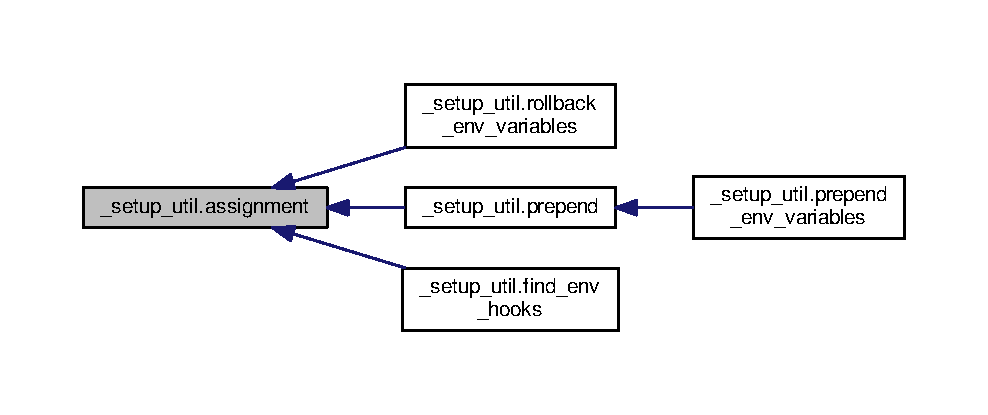
\includegraphics[width=350pt]{namespace__setup__util_ad56c24837fa4eddc63c03fbc7035628f_icgraph}
\end{center}
\end{figure}


\index{\+\_\+setup\+\_\+util@{\+\_\+setup\+\_\+util}!comment@{comment}}
\index{comment@{comment}!\+\_\+setup\+\_\+util@{\+\_\+setup\+\_\+util}}
\subsubsection[{\texorpdfstring{comment(msg)}{comment(msg)}}]{\setlength{\rightskip}{0pt plus 5cm}def \+\_\+setup\+\_\+util.\+comment (
\begin{DoxyParamCaption}
\item[{}]{msg}
\end{DoxyParamCaption}
)}\hypertarget{namespace__setup__util_abe8c95c4cfe8b1374dacd5f91d984353}{}\label{namespace__setup__util_abe8c95c4cfe8b1374dacd5f91d984353}


Definition at line 182 of file \+\_\+setup\+\_\+util.\+py.



Here is the caller graph for this function\+:
\nopagebreak
\begin{figure}[H]
\begin{center}
\leavevmode
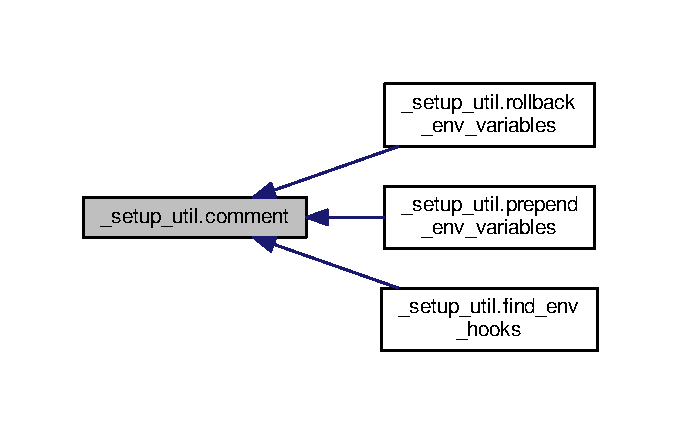
\includegraphics[width=327pt]{namespace__setup__util_abe8c95c4cfe8b1374dacd5f91d984353_icgraph}
\end{center}
\end{figure}


\index{\+\_\+setup\+\_\+util@{\+\_\+setup\+\_\+util}!find\+\_\+env\+\_\+hooks@{find\+\_\+env\+\_\+hooks}}
\index{find\+\_\+env\+\_\+hooks@{find\+\_\+env\+\_\+hooks}!\+\_\+setup\+\_\+util@{\+\_\+setup\+\_\+util}}
\subsubsection[{\texorpdfstring{find\+\_\+env\+\_\+hooks(environ, cmake\+\_\+prefix\+\_\+path)}{find_env_hooks(environ, cmake_prefix_path)}}]{\setlength{\rightskip}{0pt plus 5cm}def \+\_\+setup\+\_\+util.\+find\+\_\+env\+\_\+hooks (
\begin{DoxyParamCaption}
\item[{}]{environ, }
\item[{}]{cmake\+\_\+prefix\+\_\+path}
\end{DoxyParamCaption}
)}\hypertarget{namespace__setup__util_a73de35ca77f260af6691470342ab49ce}{}\label{namespace__setup__util_a73de35ca77f260af6691470342ab49ce}
\begin{DoxyVerb}Generate shell code with found environment hooks
for the all workspaces.
\end{DoxyVerb}
 

Definition at line 198 of file \+\_\+setup\+\_\+util.\+py.



Here is the call graph for this function\+:
\nopagebreak
\begin{figure}[H]
\begin{center}
\leavevmode
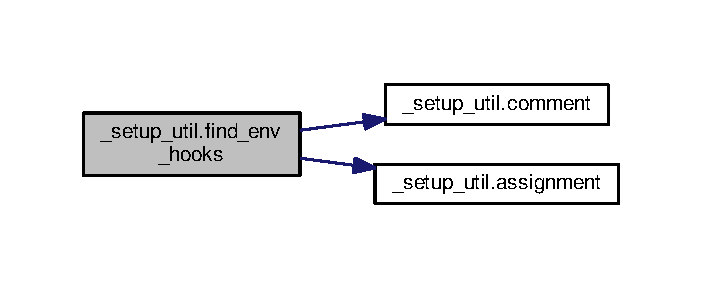
\includegraphics[width=337pt]{namespace__setup__util_a73de35ca77f260af6691470342ab49ce_cgraph}
\end{center}
\end{figure}


\index{\+\_\+setup\+\_\+util@{\+\_\+setup\+\_\+util}!prepend@{prepend}}
\index{prepend@{prepend}!\+\_\+setup\+\_\+util@{\+\_\+setup\+\_\+util}}
\subsubsection[{\texorpdfstring{prepend(environ, key, prefix)}{prepend(environ, key, prefix)}}]{\setlength{\rightskip}{0pt plus 5cm}def \+\_\+setup\+\_\+util.\+prepend (
\begin{DoxyParamCaption}
\item[{}]{environ, }
\item[{}]{key, }
\item[{}]{prefix}
\end{DoxyParamCaption}
)}\hypertarget{namespace__setup__util_ae78d86b2c4279f5b8b1acaa146c35802}{}\label{namespace__setup__util_ae78d86b2c4279f5b8b1acaa146c35802}


Definition at line 189 of file \+\_\+setup\+\_\+util.\+py.



Here is the call graph for this function\+:
\nopagebreak
\begin{figure}[H]
\begin{center}
\leavevmode
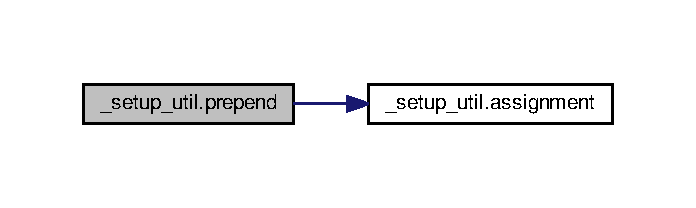
\includegraphics[width=334pt]{namespace__setup__util_ae78d86b2c4279f5b8b1acaa146c35802_cgraph}
\end{center}
\end{figure}




Here is the caller graph for this function\+:
\nopagebreak
\begin{figure}[H]
\begin{center}
\leavevmode
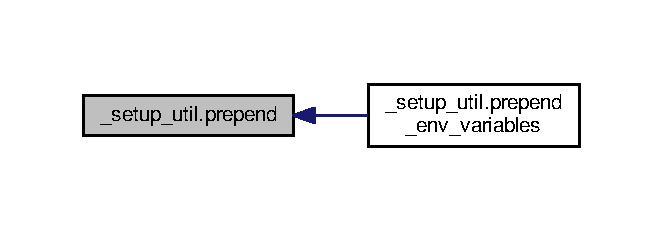
\includegraphics[width=318pt]{namespace__setup__util_ae78d86b2c4279f5b8b1acaa146c35802_icgraph}
\end{center}
\end{figure}


\index{\+\_\+setup\+\_\+util@{\+\_\+setup\+\_\+util}!prepend\+\_\+env\+\_\+variables@{prepend\+\_\+env\+\_\+variables}}
\index{prepend\+\_\+env\+\_\+variables@{prepend\+\_\+env\+\_\+variables}!\+\_\+setup\+\_\+util@{\+\_\+setup\+\_\+util}}
\subsubsection[{\texorpdfstring{prepend\+\_\+env\+\_\+variables(environ, env\+\_\+var\+\_\+subfolders, workspaces)}{prepend_env_variables(environ, env_var_subfolders, workspaces)}}]{\setlength{\rightskip}{0pt plus 5cm}def \+\_\+setup\+\_\+util.\+prepend\+\_\+env\+\_\+variables (
\begin{DoxyParamCaption}
\item[{}]{environ, }
\item[{}]{env\+\_\+var\+\_\+subfolders, }
\item[{}]{workspaces}
\end{DoxyParamCaption}
)}\hypertarget{namespace__setup__util_a832417d18b85bd1d276a87547e86f860}{}\label{namespace__setup__util_a832417d18b85bd1d276a87547e86f860}
\begin{DoxyVerb}Generate shell code to prepend environment variables
for the all workspaces.
\end{DoxyVerb}
 

Definition at line 129 of file \+\_\+setup\+\_\+util.\+py.



Here is the call graph for this function\+:
\nopagebreak
\begin{figure}[H]
\begin{center}
\leavevmode
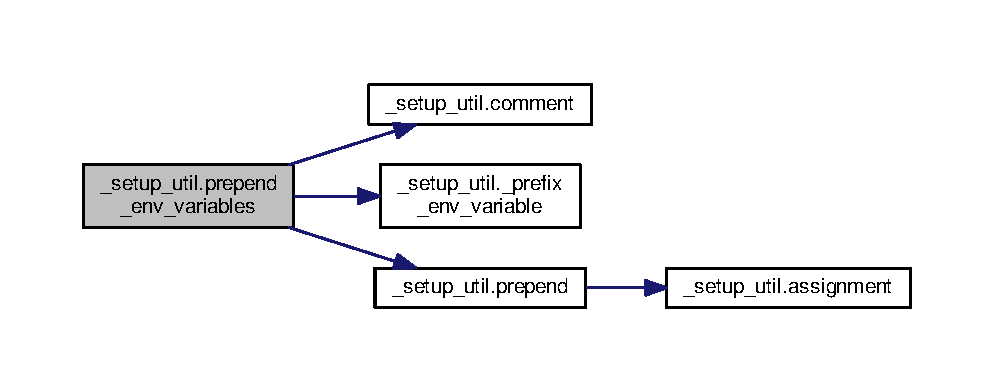
\includegraphics[width=350pt]{namespace__setup__util_a832417d18b85bd1d276a87547e86f860_cgraph}
\end{center}
\end{figure}


\index{\+\_\+setup\+\_\+util@{\+\_\+setup\+\_\+util}!rollback\+\_\+env\+\_\+variables@{rollback\+\_\+env\+\_\+variables}}
\index{rollback\+\_\+env\+\_\+variables@{rollback\+\_\+env\+\_\+variables}!\+\_\+setup\+\_\+util@{\+\_\+setup\+\_\+util}}
\subsubsection[{\texorpdfstring{rollback\+\_\+env\+\_\+variables(environ, env\+\_\+var\+\_\+subfolders)}{rollback_env_variables(environ, env_var_subfolders)}}]{\setlength{\rightskip}{0pt plus 5cm}def \+\_\+setup\+\_\+util.\+rollback\+\_\+env\+\_\+variables (
\begin{DoxyParamCaption}
\item[{}]{environ, }
\item[{}]{env\+\_\+var\+\_\+subfolders}
\end{DoxyParamCaption}
)}\hypertarget{namespace__setup__util_af3030db6102b5aa35cd354a2fb6cca03}{}\label{namespace__setup__util_af3030db6102b5aa35cd354a2fb6cca03}
\begin{DoxyVerb}Generate shell code to reset environment variables
by unrolling modifications based on all workspaces in CMAKE_PREFIX_PATH.
This does not cover modifications performed by environment hooks.
\end{DoxyVerb}
 

Definition at line 62 of file \+\_\+setup\+\_\+util.\+py.



Here is the call graph for this function\+:
\nopagebreak
\begin{figure}[H]
\begin{center}
\leavevmode
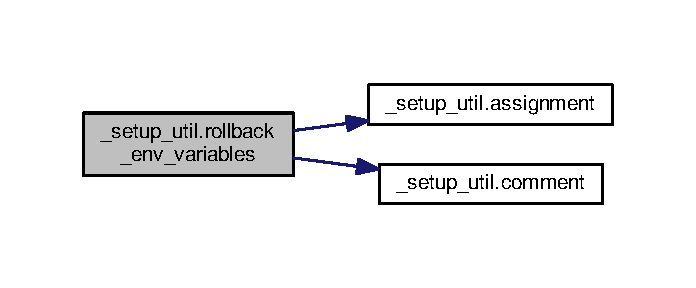
\includegraphics[width=334pt]{namespace__setup__util_af3030db6102b5aa35cd354a2fb6cca03_cgraph}
\end{center}
\end{figure}




\subsection{Variable Documentation}
\index{\+\_\+setup\+\_\+util@{\+\_\+setup\+\_\+util}!args@{args}}
\index{args@{args}!\+\_\+setup\+\_\+util@{\+\_\+setup\+\_\+util}}
\subsubsection[{\texorpdfstring{args}{args}}]{\setlength{\rightskip}{0pt plus 5cm}\+\_\+setup\+\_\+util.\+args = \+\_\+parse\+\_\+arguments()}\hypertarget{namespace__setup__util_a547963d07c6371df1c51b1384a2dec28}{}\label{namespace__setup__util_a547963d07c6371df1c51b1384a2dec28}


Definition at line 259 of file \+\_\+setup\+\_\+util.\+py.

\index{\+\_\+setup\+\_\+util@{\+\_\+setup\+\_\+util}!base\+\_\+path@{base\+\_\+path}}
\index{base\+\_\+path@{base\+\_\+path}!\+\_\+setup\+\_\+util@{\+\_\+setup\+\_\+util}}
\subsubsection[{\texorpdfstring{base\+\_\+path}{base_path}}]{\setlength{\rightskip}{0pt plus 5cm}\+\_\+setup\+\_\+util.\+base\+\_\+path = os.\+path.\+dirname(\+\_\+\+\_\+file\+\_\+\+\_\+)}\hypertarget{namespace__setup__util_a83d25140acd7788bbcb95843fe38e639}{}\label{namespace__setup__util_a83d25140acd7788bbcb95843fe38e639}


Definition at line 267 of file \+\_\+setup\+\_\+util.\+py.

\index{\+\_\+setup\+\_\+util@{\+\_\+setup\+\_\+util}!C\+A\+T\+K\+I\+N\+\_\+\+M\+A\+R\+K\+E\+R\+\_\+\+F\+I\+LE@{C\+A\+T\+K\+I\+N\+\_\+\+M\+A\+R\+K\+E\+R\+\_\+\+F\+I\+LE}}
\index{C\+A\+T\+K\+I\+N\+\_\+\+M\+A\+R\+K\+E\+R\+\_\+\+F\+I\+LE@{C\+A\+T\+K\+I\+N\+\_\+\+M\+A\+R\+K\+E\+R\+\_\+\+F\+I\+LE}!\+\_\+setup\+\_\+util@{\+\_\+setup\+\_\+util}}
\subsubsection[{\texorpdfstring{C\+A\+T\+K\+I\+N\+\_\+\+M\+A\+R\+K\+E\+R\+\_\+\+F\+I\+LE}{CATKIN_MARKER_FILE}}]{\setlength{\rightskip}{0pt plus 5cm}string \+\_\+setup\+\_\+util.\+C\+A\+T\+K\+I\+N\+\_\+\+M\+A\+R\+K\+E\+R\+\_\+\+F\+I\+LE = \textquotesingle{}.catkin\textquotesingle{}}\hypertarget{namespace__setup__util_a3fa0ca5a460a71a43cbc3d4954ab1f10}{}\label{namespace__setup__util_a3fa0ca5a460a71a43cbc3d4954ab1f10}


Definition at line 46 of file \+\_\+setup\+\_\+util.\+py.

\index{\+\_\+setup\+\_\+util@{\+\_\+setup\+\_\+util}!C\+M\+A\+K\+E\+\_\+\+P\+R\+E\+F\+I\+X\+\_\+\+P\+A\+TH@{C\+M\+A\+K\+E\+\_\+\+P\+R\+E\+F\+I\+X\+\_\+\+P\+A\+TH}}
\index{C\+M\+A\+K\+E\+\_\+\+P\+R\+E\+F\+I\+X\+\_\+\+P\+A\+TH@{C\+M\+A\+K\+E\+\_\+\+P\+R\+E\+F\+I\+X\+\_\+\+P\+A\+TH}!\+\_\+setup\+\_\+util@{\+\_\+setup\+\_\+util}}
\subsubsection[{\texorpdfstring{C\+M\+A\+K\+E\+\_\+\+P\+R\+E\+F\+I\+X\+\_\+\+P\+A\+TH}{CMAKE_PREFIX_PATH}}]{\setlength{\rightskip}{0pt plus 5cm}string \+\_\+setup\+\_\+util.\+C\+M\+A\+K\+E\+\_\+\+P\+R\+E\+F\+I\+X\+\_\+\+P\+A\+TH = \textquotesingle{}/home/jbs/catkin\+\_\+ws/devel;/opt/ros/kinetic\textquotesingle{}}\hypertarget{namespace__setup__util_a57afd3d2c076955fb715f3e72ef098eb}{}\label{namespace__setup__util_a57afd3d2c076955fb715f3e72ef098eb}


Definition at line 265 of file \+\_\+setup\+\_\+util.\+py.

\index{\+\_\+setup\+\_\+util@{\+\_\+setup\+\_\+util}!e@{e}}
\index{e@{e}!\+\_\+setup\+\_\+util@{\+\_\+setup\+\_\+util}}
\subsubsection[{\texorpdfstring{e}{e}}]{\setlength{\rightskip}{0pt plus 5cm}\+\_\+setup\+\_\+util.\+e}\hypertarget{namespace__setup__util_acdce690b925de33d6249bbbfa1109d61}{}\label{namespace__setup__util_acdce690b925de33d6249bbbfa1109d61}


Definition at line 261 of file \+\_\+setup\+\_\+util.\+py.

\index{\+\_\+setup\+\_\+util@{\+\_\+setup\+\_\+util}!E\+N\+V\+\_\+\+V\+A\+R\+\_\+\+S\+U\+B\+F\+O\+L\+D\+E\+RS@{E\+N\+V\+\_\+\+V\+A\+R\+\_\+\+S\+U\+B\+F\+O\+L\+D\+E\+RS}}
\index{E\+N\+V\+\_\+\+V\+A\+R\+\_\+\+S\+U\+B\+F\+O\+L\+D\+E\+RS@{E\+N\+V\+\_\+\+V\+A\+R\+\_\+\+S\+U\+B\+F\+O\+L\+D\+E\+RS}!\+\_\+setup\+\_\+util@{\+\_\+setup\+\_\+util}}
\subsubsection[{\texorpdfstring{E\+N\+V\+\_\+\+V\+A\+R\+\_\+\+S\+U\+B\+F\+O\+L\+D\+E\+RS}{ENV_VAR_SUBFOLDERS}}]{\setlength{\rightskip}{0pt plus 5cm}dictionary \+\_\+setup\+\_\+util.\+E\+N\+V\+\_\+\+V\+A\+R\+\_\+\+S\+U\+B\+F\+O\+L\+D\+E\+RS}\hypertarget{namespace__setup__util_aa31804f1be8660156ce9394b33c68dc4}{}\label{namespace__setup__util_aa31804f1be8660156ce9394b33c68dc4}
{\bfseries Initial value\+:}
\begin{DoxyCode}
1 = \{
2     \textcolor{stringliteral}{'CMAKE\_PREFIX\_PATH'}: \textcolor{stringliteral}{''},
3     \textcolor{stringliteral}{'LD\_LIBRARY\_PATH'} \textcolor{keywordflow}{if} \textcolor{keywordflow}{not} IS\_DARWIN \textcolor{keywordflow}{else} \textcolor{stringliteral}{'DYLD\_LIBRARY\_PATH'}: [\textcolor{stringliteral}{'lib'}, os.path.join(\textcolor{stringliteral}{'lib'}, \textcolor{stringliteral}{'
      x86\_64-linux-gnu'})],
4     \textcolor{stringliteral}{'PATH'}: \textcolor{stringliteral}{'bin'},
5     \textcolor{stringliteral}{'PKG\_CONFIG\_PATH'}: [os.path.join(\textcolor{stringliteral}{'lib'}, \textcolor{stringliteral}{'pkgconfig'}), os.path.join(\textcolor{stringliteral}{'lib'}, \textcolor{stringliteral}{'x86\_64-linux-gnu'}, \textcolor{stringliteral}{'
      pkgconfig'})],
6     \textcolor{stringliteral}{'PYTHONPATH'}: \textcolor{stringliteral}{'lib/python2.7/dist-packages'},
7 \}
\end{DoxyCode}


Definition at line 53 of file \+\_\+setup\+\_\+util.\+py.

\index{\+\_\+setup\+\_\+util@{\+\_\+setup\+\_\+util}!environ@{environ}}
\index{environ@{environ}!\+\_\+setup\+\_\+util@{\+\_\+setup\+\_\+util}}
\subsubsection[{\texorpdfstring{environ}{environ}}]{\setlength{\rightskip}{0pt plus 5cm}\+\_\+setup\+\_\+util.\+environ = dict(os.\+environ)}\hypertarget{namespace__setup__util_a9a935bdd9ee1aa0327161025bb18c136}{}\label{namespace__setup__util_a9a935bdd9ee1aa0327161025bb18c136}


Definition at line 272 of file \+\_\+setup\+\_\+util.\+py.

\index{\+\_\+setup\+\_\+util@{\+\_\+setup\+\_\+util}!file@{file}}
\index{file@{file}!\+\_\+setup\+\_\+util@{\+\_\+setup\+\_\+util}}
\subsubsection[{\texorpdfstring{file}{file}}]{\setlength{\rightskip}{0pt plus 5cm}\+\_\+setup\+\_\+util.\+file}\hypertarget{namespace__setup__util_aea63a1b32cc79bc3d872ab7cb30dd07e}{}\label{namespace__setup__util_aea63a1b32cc79bc3d872ab7cb30dd07e}


Definition at line 261 of file \+\_\+setup\+\_\+util.\+py.

\index{\+\_\+setup\+\_\+util@{\+\_\+setup\+\_\+util}!I\+S\+\_\+\+D\+A\+R\+W\+IN@{I\+S\+\_\+\+D\+A\+R\+W\+IN}}
\index{I\+S\+\_\+\+D\+A\+R\+W\+IN@{I\+S\+\_\+\+D\+A\+R\+W\+IN}!\+\_\+setup\+\_\+util@{\+\_\+setup\+\_\+util}}
\subsubsection[{\texorpdfstring{I\+S\+\_\+\+D\+A\+R\+W\+IN}{IS_DARWIN}}]{\setlength{\rightskip}{0pt plus 5cm}tuple \+\_\+setup\+\_\+util.\+I\+S\+\_\+\+D\+A\+R\+W\+IN = ({\bf system} == \textquotesingle{}Darwin\textquotesingle{})}\hypertarget{namespace__setup__util_aecbb100ce6f94bb3c7e16d58fde05f96}{}\label{namespace__setup__util_aecbb100ce6f94bb3c7e16d58fde05f96}


Definition at line 49 of file \+\_\+setup\+\_\+util.\+py.

\index{\+\_\+setup\+\_\+util@{\+\_\+setup\+\_\+util}!I\+S\+\_\+\+W\+I\+N\+D\+O\+WS@{I\+S\+\_\+\+W\+I\+N\+D\+O\+WS}}
\index{I\+S\+\_\+\+W\+I\+N\+D\+O\+WS@{I\+S\+\_\+\+W\+I\+N\+D\+O\+WS}!\+\_\+setup\+\_\+util@{\+\_\+setup\+\_\+util}}
\subsubsection[{\texorpdfstring{I\+S\+\_\+\+W\+I\+N\+D\+O\+WS}{IS_WINDOWS}}]{\setlength{\rightskip}{0pt plus 5cm}tuple \+\_\+setup\+\_\+util.\+I\+S\+\_\+\+W\+I\+N\+D\+O\+WS = ({\bf system} == \textquotesingle{}Windows\textquotesingle{})}\hypertarget{namespace__setup__util_a6fe69c2dbd92959b6651a28cbb846e6e}{}\label{namespace__setup__util_a6fe69c2dbd92959b6651a28cbb846e6e}


Definition at line 50 of file \+\_\+setup\+\_\+util.\+py.

\index{\+\_\+setup\+\_\+util@{\+\_\+setup\+\_\+util}!lines@{lines}}
\index{lines@{lines}!\+\_\+setup\+\_\+util@{\+\_\+setup\+\_\+util}}
\subsubsection[{\texorpdfstring{lines}{lines}}]{\setlength{\rightskip}{0pt plus 5cm}list \+\_\+setup\+\_\+util.\+lines = \mbox{[}$\,$\mbox{]}}\hypertarget{namespace__setup__util_a8618d8be5f729d4c9696daa5e083a001}{}\label{namespace__setup__util_a8618d8be5f729d4c9696daa5e083a001}


Definition at line 273 of file \+\_\+setup\+\_\+util.\+py.

\index{\+\_\+setup\+\_\+util@{\+\_\+setup\+\_\+util}!system@{system}}
\index{system@{system}!\+\_\+setup\+\_\+util@{\+\_\+setup\+\_\+util}}
\subsubsection[{\texorpdfstring{system}{system}}]{\setlength{\rightskip}{0pt plus 5cm}\+\_\+setup\+\_\+util.\+system = platform.\+system()}\hypertarget{namespace__setup__util_ae9fca6a80a6923f4580be72f68fee325}{}\label{namespace__setup__util_ae9fca6a80a6923f4580be72f68fee325}


Definition at line 48 of file \+\_\+setup\+\_\+util.\+py.


\hypertarget{namespacechaser}{}\section{chaser Namespace Reference}
\label{namespacechaser}\index{chaser@{chaser}}
\subsection*{Classes}
\begin{DoxyCompactItemize}
\item 
struct \hyperlink{structchaser_1_1_preplanner_params}{Preplanner\+Params}
\item 
struct \hyperlink{structchaser_1_1_smoothplanner_params}{Smoothplanner\+Params}
\end{DoxyCompactItemize}

\hypertarget{namespacegenerate__cached__setup}{}\section{generate\+\_\+cached\+\_\+setup Namespace Reference}
\label{namespacegenerate__cached__setup}\index{generate\+\_\+cached\+\_\+setup@{generate\+\_\+cached\+\_\+setup}}
\subsection*{Variables}
\begin{DoxyCompactItemize}
\item 
\hyperlink{namespacegenerate__cached__setup_a72579fd01529a79bab20d99291889d3f}{python\+\_\+path} = os.\+path.\+join(workspace, \textquotesingle{}lib/python2.\+7/dist-\/packages\textquotesingle{})
\item 
\hyperlink{namespacegenerate__cached__setup_a52601295006f2366a311c4453d8f2f2e}{code} = generate\+\_\+environment\+\_\+script(\textquotesingle{}/home/jbs/catkin\+\_\+ws/src/auto\+\_\+chaser/build/devel/env.\+sh\textquotesingle{})
\item 
string \hyperlink{namespacegenerate__cached__setup_a0265aee5075ee1eb701ff69c98ad6793}{output\+\_\+filename} = \textquotesingle{}/home/jbs/catkin\+\_\+ws/src/auto\+\_\+chaser/build/catkin\+\_\+generated/setup\+\_\+cached.\+sh\textquotesingle{}
\item 
\hyperlink{namespacegenerate__cached__setup_a10081e5abedae9bd46dd91202096e789}{mode} = os.\+stat(\hyperlink{namespacegenerate__cached__setup_a0265aee5075ee1eb701ff69c98ad6793}{output\+\_\+filename}).st\+\_\+mode
\end{DoxyCompactItemize}


\subsection{Variable Documentation}
\index{generate\+\_\+cached\+\_\+setup@{generate\+\_\+cached\+\_\+setup}!code@{code}}
\index{code@{code}!generate\+\_\+cached\+\_\+setup@{generate\+\_\+cached\+\_\+setup}}
\subsubsection[{\texorpdfstring{code}{code}}]{\setlength{\rightskip}{0pt plus 5cm}generate\+\_\+cached\+\_\+setup.\+code = generate\+\_\+environment\+\_\+script(\textquotesingle{}/home/jbs/catkin\+\_\+ws/src/auto\+\_\+chaser/build/devel/env.\+sh\textquotesingle{})}\hypertarget{namespacegenerate__cached__setup_a52601295006f2366a311c4453d8f2f2e}{}\label{namespacegenerate__cached__setup_a52601295006f2366a311c4453d8f2f2e}
\index{generate\+\_\+cached\+\_\+setup@{generate\+\_\+cached\+\_\+setup}!mode@{mode}}
\index{mode@{mode}!generate\+\_\+cached\+\_\+setup@{generate\+\_\+cached\+\_\+setup}}
\subsubsection[{\texorpdfstring{mode}{mode}}]{\setlength{\rightskip}{0pt plus 5cm}generate\+\_\+cached\+\_\+setup.\+mode = os.\+stat({\bf output\+\_\+filename}).st\+\_\+mode}\hypertarget{namespacegenerate__cached__setup_a10081e5abedae9bd46dd91202096e789}{}\label{namespacegenerate__cached__setup_a10081e5abedae9bd46dd91202096e789}
\index{generate\+\_\+cached\+\_\+setup@{generate\+\_\+cached\+\_\+setup}!output\+\_\+filename@{output\+\_\+filename}}
\index{output\+\_\+filename@{output\+\_\+filename}!generate\+\_\+cached\+\_\+setup@{generate\+\_\+cached\+\_\+setup}}
\subsubsection[{\texorpdfstring{output\+\_\+filename}{output_filename}}]{\setlength{\rightskip}{0pt plus 5cm}string generate\+\_\+cached\+\_\+setup.\+output\+\_\+filename = \textquotesingle{}/home/jbs/catkin\+\_\+ws/src/auto\+\_\+chaser/build/catkin\+\_\+generated/setup\+\_\+cached.\+sh\textquotesingle{}}\hypertarget{namespacegenerate__cached__setup_a0265aee5075ee1eb701ff69c98ad6793}{}\label{namespacegenerate__cached__setup_a0265aee5075ee1eb701ff69c98ad6793}
\index{generate\+\_\+cached\+\_\+setup@{generate\+\_\+cached\+\_\+setup}!python\+\_\+path@{python\+\_\+path}}
\index{python\+\_\+path@{python\+\_\+path}!generate\+\_\+cached\+\_\+setup@{generate\+\_\+cached\+\_\+setup}}
\subsubsection[{\texorpdfstring{python\+\_\+path}{python_path}}]{\setlength{\rightskip}{0pt plus 5cm}generate\+\_\+cached\+\_\+setup.\+python\+\_\+path = os.\+path.\+join(workspace, \textquotesingle{}lib/python2.\+7/dist-\/packages\textquotesingle{})}\hypertarget{namespacegenerate__cached__setup_a72579fd01529a79bab20d99291889d3f}{}\label{namespacegenerate__cached__setup_a72579fd01529a79bab20d99291889d3f}

\hypertarget{namespacepkg}{}\section{pkg Namespace Reference}
\label{namespacepkg}\index{pkg@{pkg}}
\subsection*{Variables}
\begin{DoxyCompactItemize}
\item 
string \hyperlink{namespacepkg_ae26c7a5a06b7d738f4d210ca449e6bee}{C\+A\+T\+K\+I\+N\+\_\+\+P\+A\+C\+K\+A\+G\+E\+\_\+\+P\+R\+E\+F\+IX} = \char`\"{}\char`\"{}
\item 
string \hyperlink{namespacepkg_a2760bf8266ff58da440f65ee91b203ab}{P\+R\+O\+J\+E\+C\+T\+\_\+\+P\+K\+G\+\_\+\+C\+O\+N\+F\+I\+G\+\_\+\+I\+N\+C\+L\+U\+D\+E\+\_\+\+D\+I\+RS} = \char`\"{}/home/jbs/catkin\+\_\+ws/src/auto\+\_\+chaser/include\char`\"{}
\item 
string \hyperlink{namespacepkg_a17c18447fad253ee1c0d76deec88028c}{P\+R\+O\+J\+E\+C\+T\+\_\+\+C\+A\+T\+K\+I\+N\+\_\+\+D\+E\+P\+E\+N\+DS} = \char`\"{}\char`\"{}
\item 
string \hyperlink{namespacepkg_a433e30cecb4a0123a7c4b384d168e336}{P\+K\+G\+\_\+\+C\+O\+N\+F\+I\+G\+\_\+\+L\+I\+B\+R\+A\+R\+I\+E\+S\+\_\+\+W\+I\+T\+H\+\_\+\+P\+R\+E\+F\+IX} = \char`\"{}-\/ltraj\+\_\+gen\+\_\+chasing\char`\"{}
\item 
string \hyperlink{namespacepkg_a7dfbe99257c26f5e4a3a5483995d9ddc}{P\+R\+O\+J\+E\+C\+T\+\_\+\+N\+A\+ME} = \char`\"{}auto\+\_\+chaser\char`\"{}
\item 
string \hyperlink{namespacepkg_a3f0f1b4bc03c596525e025539ca4332f}{P\+R\+O\+J\+E\+C\+T\+\_\+\+S\+P\+A\+C\+E\+\_\+\+D\+IR} = \char`\"{}/home/jbs/catkin\+\_\+ws/src/auto\+\_\+chaser/build/devel\char`\"{}
\item 
string \hyperlink{namespacepkg_ab1037914b9286bb61855131c06149648}{P\+R\+O\+J\+E\+C\+T\+\_\+\+V\+E\+R\+S\+I\+ON} = \char`\"{}0.\+0.\+0\char`\"{}
\end{DoxyCompactItemize}


\subsection{Variable Documentation}
\index{pkg@{pkg}!C\+A\+T\+K\+I\+N\+\_\+\+P\+A\+C\+K\+A\+G\+E\+\_\+\+P\+R\+E\+F\+IX@{C\+A\+T\+K\+I\+N\+\_\+\+P\+A\+C\+K\+A\+G\+E\+\_\+\+P\+R\+E\+F\+IX}}
\index{C\+A\+T\+K\+I\+N\+\_\+\+P\+A\+C\+K\+A\+G\+E\+\_\+\+P\+R\+E\+F\+IX@{C\+A\+T\+K\+I\+N\+\_\+\+P\+A\+C\+K\+A\+G\+E\+\_\+\+P\+R\+E\+F\+IX}!pkg@{pkg}}
\subsubsection[{\texorpdfstring{C\+A\+T\+K\+I\+N\+\_\+\+P\+A\+C\+K\+A\+G\+E\+\_\+\+P\+R\+E\+F\+IX}{CATKIN_PACKAGE_PREFIX}}]{\setlength{\rightskip}{0pt plus 5cm}string pkg.\+C\+A\+T\+K\+I\+N\+\_\+\+P\+A\+C\+K\+A\+G\+E\+\_\+\+P\+R\+E\+F\+IX = \char`\"{}\char`\"{}}\hypertarget{namespacepkg_ae26c7a5a06b7d738f4d210ca449e6bee}{}\label{namespacepkg_ae26c7a5a06b7d738f4d210ca449e6bee}


Definition at line 2 of file pkg.\+develspace.\+context.\+pc.\+py.

\index{pkg@{pkg}!P\+K\+G\+\_\+\+C\+O\+N\+F\+I\+G\+\_\+\+L\+I\+B\+R\+A\+R\+I\+E\+S\+\_\+\+W\+I\+T\+H\+\_\+\+P\+R\+E\+F\+IX@{P\+K\+G\+\_\+\+C\+O\+N\+F\+I\+G\+\_\+\+L\+I\+B\+R\+A\+R\+I\+E\+S\+\_\+\+W\+I\+T\+H\+\_\+\+P\+R\+E\+F\+IX}}
\index{P\+K\+G\+\_\+\+C\+O\+N\+F\+I\+G\+\_\+\+L\+I\+B\+R\+A\+R\+I\+E\+S\+\_\+\+W\+I\+T\+H\+\_\+\+P\+R\+E\+F\+IX@{P\+K\+G\+\_\+\+C\+O\+N\+F\+I\+G\+\_\+\+L\+I\+B\+R\+A\+R\+I\+E\+S\+\_\+\+W\+I\+T\+H\+\_\+\+P\+R\+E\+F\+IX}!pkg@{pkg}}
\subsubsection[{\texorpdfstring{P\+K\+G\+\_\+\+C\+O\+N\+F\+I\+G\+\_\+\+L\+I\+B\+R\+A\+R\+I\+E\+S\+\_\+\+W\+I\+T\+H\+\_\+\+P\+R\+E\+F\+IX}{PKG_CONFIG_LIBRARIES_WITH_PREFIX}}]{\setlength{\rightskip}{0pt plus 5cm}string pkg.\+P\+K\+G\+\_\+\+C\+O\+N\+F\+I\+G\+\_\+\+L\+I\+B\+R\+A\+R\+I\+E\+S\+\_\+\+W\+I\+T\+H\+\_\+\+P\+R\+E\+F\+IX = \char`\"{}-\/ltraj\+\_\+gen\+\_\+chasing\char`\"{}}\hypertarget{namespacepkg_a433e30cecb4a0123a7c4b384d168e336}{}\label{namespacepkg_a433e30cecb4a0123a7c4b384d168e336}


Definition at line 5 of file pkg.\+develspace.\+context.\+pc.\+py.

\index{pkg@{pkg}!P\+R\+O\+J\+E\+C\+T\+\_\+\+C\+A\+T\+K\+I\+N\+\_\+\+D\+E\+P\+E\+N\+DS@{P\+R\+O\+J\+E\+C\+T\+\_\+\+C\+A\+T\+K\+I\+N\+\_\+\+D\+E\+P\+E\+N\+DS}}
\index{P\+R\+O\+J\+E\+C\+T\+\_\+\+C\+A\+T\+K\+I\+N\+\_\+\+D\+E\+P\+E\+N\+DS@{P\+R\+O\+J\+E\+C\+T\+\_\+\+C\+A\+T\+K\+I\+N\+\_\+\+D\+E\+P\+E\+N\+DS}!pkg@{pkg}}
\subsubsection[{\texorpdfstring{P\+R\+O\+J\+E\+C\+T\+\_\+\+C\+A\+T\+K\+I\+N\+\_\+\+D\+E\+P\+E\+N\+DS}{PROJECT_CATKIN_DEPENDS}}]{\setlength{\rightskip}{0pt plus 5cm}string pkg.\+P\+R\+O\+J\+E\+C\+T\+\_\+\+C\+A\+T\+K\+I\+N\+\_\+\+D\+E\+P\+E\+N\+DS = \char`\"{}\char`\"{}}\hypertarget{namespacepkg_a17c18447fad253ee1c0d76deec88028c}{}\label{namespacepkg_a17c18447fad253ee1c0d76deec88028c}


Definition at line 4 of file pkg.\+develspace.\+context.\+pc.\+py.

\index{pkg@{pkg}!P\+R\+O\+J\+E\+C\+T\+\_\+\+N\+A\+ME@{P\+R\+O\+J\+E\+C\+T\+\_\+\+N\+A\+ME}}
\index{P\+R\+O\+J\+E\+C\+T\+\_\+\+N\+A\+ME@{P\+R\+O\+J\+E\+C\+T\+\_\+\+N\+A\+ME}!pkg@{pkg}}
\subsubsection[{\texorpdfstring{P\+R\+O\+J\+E\+C\+T\+\_\+\+N\+A\+ME}{PROJECT_NAME}}]{\setlength{\rightskip}{0pt plus 5cm}string pkg.\+P\+R\+O\+J\+E\+C\+T\+\_\+\+N\+A\+ME = \char`\"{}auto\+\_\+chaser\char`\"{}}\hypertarget{namespacepkg_a7dfbe99257c26f5e4a3a5483995d9ddc}{}\label{namespacepkg_a7dfbe99257c26f5e4a3a5483995d9ddc}


Definition at line 6 of file pkg.\+develspace.\+context.\+pc.\+py.

\index{pkg@{pkg}!P\+R\+O\+J\+E\+C\+T\+\_\+\+P\+K\+G\+\_\+\+C\+O\+N\+F\+I\+G\+\_\+\+I\+N\+C\+L\+U\+D\+E\+\_\+\+D\+I\+RS@{P\+R\+O\+J\+E\+C\+T\+\_\+\+P\+K\+G\+\_\+\+C\+O\+N\+F\+I\+G\+\_\+\+I\+N\+C\+L\+U\+D\+E\+\_\+\+D\+I\+RS}}
\index{P\+R\+O\+J\+E\+C\+T\+\_\+\+P\+K\+G\+\_\+\+C\+O\+N\+F\+I\+G\+\_\+\+I\+N\+C\+L\+U\+D\+E\+\_\+\+D\+I\+RS@{P\+R\+O\+J\+E\+C\+T\+\_\+\+P\+K\+G\+\_\+\+C\+O\+N\+F\+I\+G\+\_\+\+I\+N\+C\+L\+U\+D\+E\+\_\+\+D\+I\+RS}!pkg@{pkg}}
\subsubsection[{\texorpdfstring{P\+R\+O\+J\+E\+C\+T\+\_\+\+P\+K\+G\+\_\+\+C\+O\+N\+F\+I\+G\+\_\+\+I\+N\+C\+L\+U\+D\+E\+\_\+\+D\+I\+RS}{PROJECT_PKG_CONFIG_INCLUDE_DIRS}}]{\setlength{\rightskip}{0pt plus 5cm}string pkg.\+P\+R\+O\+J\+E\+C\+T\+\_\+\+P\+K\+G\+\_\+\+C\+O\+N\+F\+I\+G\+\_\+\+I\+N\+C\+L\+U\+D\+E\+\_\+\+D\+I\+RS = \char`\"{}/home/jbs/catkin\+\_\+ws/src/auto\+\_\+chaser/include\char`\"{}}\hypertarget{namespacepkg_a2760bf8266ff58da440f65ee91b203ab}{}\label{namespacepkg_a2760bf8266ff58da440f65ee91b203ab}


Definition at line 3 of file pkg.\+develspace.\+context.\+pc.\+py.

\index{pkg@{pkg}!P\+R\+O\+J\+E\+C\+T\+\_\+\+S\+P\+A\+C\+E\+\_\+\+D\+IR@{P\+R\+O\+J\+E\+C\+T\+\_\+\+S\+P\+A\+C\+E\+\_\+\+D\+IR}}
\index{P\+R\+O\+J\+E\+C\+T\+\_\+\+S\+P\+A\+C\+E\+\_\+\+D\+IR@{P\+R\+O\+J\+E\+C\+T\+\_\+\+S\+P\+A\+C\+E\+\_\+\+D\+IR}!pkg@{pkg}}
\subsubsection[{\texorpdfstring{P\+R\+O\+J\+E\+C\+T\+\_\+\+S\+P\+A\+C\+E\+\_\+\+D\+IR}{PROJECT_SPACE_DIR}}]{\setlength{\rightskip}{0pt plus 5cm}string pkg.\+P\+R\+O\+J\+E\+C\+T\+\_\+\+S\+P\+A\+C\+E\+\_\+\+D\+IR = \char`\"{}/home/jbs/catkin\+\_\+ws/src/auto\+\_\+chaser/build/devel\char`\"{}}\hypertarget{namespacepkg_a3f0f1b4bc03c596525e025539ca4332f}{}\label{namespacepkg_a3f0f1b4bc03c596525e025539ca4332f}


Definition at line 7 of file pkg.\+develspace.\+context.\+pc.\+py.

\index{pkg@{pkg}!P\+R\+O\+J\+E\+C\+T\+\_\+\+V\+E\+R\+S\+I\+ON@{P\+R\+O\+J\+E\+C\+T\+\_\+\+V\+E\+R\+S\+I\+ON}}
\index{P\+R\+O\+J\+E\+C\+T\+\_\+\+V\+E\+R\+S\+I\+ON@{P\+R\+O\+J\+E\+C\+T\+\_\+\+V\+E\+R\+S\+I\+ON}!pkg@{pkg}}
\subsubsection[{\texorpdfstring{P\+R\+O\+J\+E\+C\+T\+\_\+\+V\+E\+R\+S\+I\+ON}{PROJECT_VERSION}}]{\setlength{\rightskip}{0pt plus 5cm}string pkg.\+P\+R\+O\+J\+E\+C\+T\+\_\+\+V\+E\+R\+S\+I\+ON = \char`\"{}0.\+0.\+0\char`\"{}}\hypertarget{namespacepkg_ab1037914b9286bb61855131c06149648}{}\label{namespacepkg_ab1037914b9286bb61855131c06149648}


Definition at line 8 of file pkg.\+develspace.\+context.\+pc.\+py.


\hypertarget{namespace_ui}{}\section{Ui Namespace Reference}
\label{namespace_ui}\index{Ui@{Ui}}
\subsection*{Classes}
\begin{DoxyCompactItemize}
\item 
class \hyperlink{class_ui_1_1_main_window}{Main\+Window}
\end{DoxyCompactItemize}

\chapter{Class Documentation}
\hypertarget{class_chaser}{}\section{Chaser Class Reference}
\label{class_chaser}\index{Chaser@{Chaser}}


{\ttfamily \#include $<$Chaser.\+h$>$}

\subsection*{Public Member Functions}
\begin{DoxyCompactItemize}
\item 
\hyperlink{class_chaser_ae1179fa7b77db9c80468f88222e32f09}{Chaser} ()
\item 
void \hyperlink{class_chaser_a3538485980643e885755608e4297d1f6}{init} (ros\+::\+Node\+Handle nh)
\item 
bool \hyperlink{class_chaser_a8feeca68466b9b4576ee9c99b624dfc5}{chase\+\_\+update} (\hyperlink{struct_grid_field}{Grid\+Field} $\ast$global\+\_\+edf, vector$<$ Point $>$ target\+\_\+pnts, Point chaser\+\_\+x0, Twist chaser\+\_\+v0, Twist chaser\+\_\+a0, Time\+Series knots)
\item 
void \hyperlink{class_chaser_a7d736728bb5327acf0d334d7d4b1b844}{session} (double t)
\item 
Point \hyperlink{class_chaser_a6dca60b8af1c63eff3235515255cf355}{eval\+\_\+point} (double t\+\_\+eval)
\item 
Twist \hyperlink{class_chaser_a208374e7b85f9a35c1c00ec4f1ec65c3}{eval\+\_\+velocity} (double t\+\_\+eval)
\item 
Twist \hyperlink{class_chaser_a2fe36102d5a9befcb4c6ada3375260ed}{eval\+\_\+acceleration} (double t\+\_\+eval)
\item 
Point \hyperlink{class_chaser_a7a42e3dd3ca45e343652318e591f87d1}{get\+\_\+control\+\_\+point} (double t\+\_\+eval)
\begin{DoxyCompactList}\small\item\em obtains the latest control point. yaw will be selected from wrapper with information of target \end{DoxyCompactList}\item 
double \hyperlink{class_chaser_aaa7ce7ea18761dd1513cf9e85c6b4e48}{get\+\_\+hovering\+\_\+z} ()
\end{DoxyCompactItemize}
\subsection*{Public Attributes}
\begin{DoxyCompactItemize}
\item 
bool \hyperlink{class_chaser_a53af032471ad6bdc828c4eae78085813}{is\+\_\+complete\+\_\+chasing\+\_\+path}
\item 
bool \hyperlink{class_chaser_a33b880dd48d1d983001fa93ba1a1184f}{is\+\_\+log}
\item 
string \hyperlink{class_chaser_a9d9ad4c7ca00bcda38d2bc809f3e7654}{log\+\_\+dir}
\end{DoxyCompactItemize}


\subsection{Detailed Description}


Definition at line 5 of file Chaser.\+h.



\subsection{Constructor \& Destructor Documentation}
\index{Chaser@{Chaser}!Chaser@{Chaser}}
\index{Chaser@{Chaser}!Chaser@{Chaser}}
\subsubsection[{\texorpdfstring{Chaser()}{Chaser()}}]{\setlength{\rightskip}{0pt plus 5cm}Chaser\+::\+Chaser (
\begin{DoxyParamCaption}
{}
\end{DoxyParamCaption}
)}\hypertarget{class_chaser_ae1179fa7b77db9c80468f88222e32f09}{}\label{class_chaser_ae1179fa7b77db9c80468f88222e32f09}


Definition at line 3 of file Chaser.\+cpp.



\subsection{Member Function Documentation}
\index{Chaser@{Chaser}!chase\+\_\+update@{chase\+\_\+update}}
\index{chase\+\_\+update@{chase\+\_\+update}!Chaser@{Chaser}}
\subsubsection[{\texorpdfstring{chase\+\_\+update(\+Grid\+Field $\ast$global\+\_\+edf, vector$<$ Point $>$ target\+\_\+pnts, Point chaser\+\_\+x0, Twist chaser\+\_\+v0, Twist chaser\+\_\+a0, Time\+Series knots)}{chase_update(GridField *global_edf, vector< Point > target_pnts, Point chaser_x0, Twist chaser_v0, Twist chaser_a0, TimeSeries knots)}}]{\setlength{\rightskip}{0pt plus 5cm}bool Chaser\+::chase\+\_\+update (
\begin{DoxyParamCaption}
\item[{{\bf Grid\+Field} $\ast$}]{global\+\_\+edf, }
\item[{vector$<$ Point $>$}]{target\+\_\+pnts, }
\item[{Point}]{chaser\+\_\+x0, }
\item[{Twist}]{chaser\+\_\+v0, }
\item[{Twist}]{chaser\+\_\+a0, }
\item[{Time\+Series}]{knots}
\end{DoxyParamCaption}
)}\hypertarget{class_chaser_a8feeca68466b9b4576ee9c99b624dfc5}{}\label{class_chaser_a8feeca68466b9b4576ee9c99b624dfc5}


Definition at line 26 of file Chaser.\+cpp.



Here is the call graph for this function\+:
\nopagebreak
\begin{figure}[H]
\begin{center}
\leavevmode
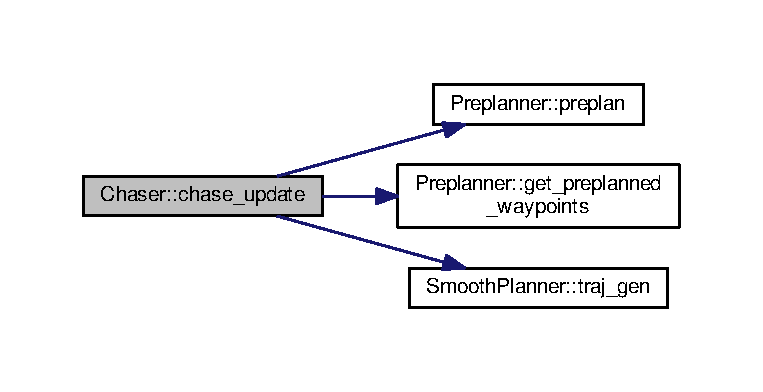
\includegraphics[width=350pt]{class_chaser_a8feeca68466b9b4576ee9c99b624dfc5_cgraph}
\end{center}
\end{figure}


\index{Chaser@{Chaser}!eval\+\_\+acceleration@{eval\+\_\+acceleration}}
\index{eval\+\_\+acceleration@{eval\+\_\+acceleration}!Chaser@{Chaser}}
\subsubsection[{\texorpdfstring{eval\+\_\+acceleration(double t\+\_\+eval)}{eval_acceleration(double t_eval)}}]{\setlength{\rightskip}{0pt plus 5cm}Twist Chaser\+::eval\+\_\+acceleration (
\begin{DoxyParamCaption}
\item[{double}]{t\+\_\+eval}
\end{DoxyParamCaption}
)}\hypertarget{class_chaser_a2fe36102d5a9befcb4c6ada3375260ed}{}\label{class_chaser_a2fe36102d5a9befcb4c6ada3375260ed}


Definition at line 86 of file Chaser.\+cpp.

\index{Chaser@{Chaser}!eval\+\_\+point@{eval\+\_\+point}}
\index{eval\+\_\+point@{eval\+\_\+point}!Chaser@{Chaser}}
\subsubsection[{\texorpdfstring{eval\+\_\+point(double t\+\_\+eval)}{eval_point(double t_eval)}}]{\setlength{\rightskip}{0pt plus 5cm}Point Chaser\+::eval\+\_\+point (
\begin{DoxyParamCaption}
\item[{double}]{t\+\_\+eval}
\end{DoxyParamCaption}
)}\hypertarget{class_chaser_a6dca60b8af1c63eff3235515255cf355}{}\label{class_chaser_a6dca60b8af1c63eff3235515255cf355}


Definition at line 77 of file Chaser.\+cpp.

\index{Chaser@{Chaser}!eval\+\_\+velocity@{eval\+\_\+velocity}}
\index{eval\+\_\+velocity@{eval\+\_\+velocity}!Chaser@{Chaser}}
\subsubsection[{\texorpdfstring{eval\+\_\+velocity(double t\+\_\+eval)}{eval_velocity(double t_eval)}}]{\setlength{\rightskip}{0pt plus 5cm}Twist Chaser\+::eval\+\_\+velocity (
\begin{DoxyParamCaption}
\item[{double}]{t\+\_\+eval}
\end{DoxyParamCaption}
)}\hypertarget{class_chaser_a208374e7b85f9a35c1c00ec4f1ec65c3}{}\label{class_chaser_a208374e7b85f9a35c1c00ec4f1ec65c3}


Definition at line 82 of file Chaser.\+cpp.

\index{Chaser@{Chaser}!get\+\_\+control\+\_\+point@{get\+\_\+control\+\_\+point}}
\index{get\+\_\+control\+\_\+point@{get\+\_\+control\+\_\+point}!Chaser@{Chaser}}
\subsubsection[{\texorpdfstring{get\+\_\+control\+\_\+point(double t\+\_\+eval)}{get_control_point(double t_eval)}}]{\setlength{\rightskip}{0pt plus 5cm}Point Chaser\+::get\+\_\+control\+\_\+point (
\begin{DoxyParamCaption}
\item[{double}]{t\+\_\+eval}
\end{DoxyParamCaption}
)}\hypertarget{class_chaser_a7a42e3dd3ca45e343652318e591f87d1}{}\label{class_chaser_a7a42e3dd3ca45e343652318e591f87d1}


obtains the latest control point. yaw will be selected from wrapper with information of target 


\begin{DoxyParams}{Parameters}
{\em t\+\_\+eval} & evaluation time \\
\hline
\end{DoxyParams}
\begin{DoxyReturn}{Returns}
Point the control point 
\end{DoxyReturn}


Definition at line 97 of file Chaser.\+cpp.

\index{Chaser@{Chaser}!get\+\_\+hovering\+\_\+z@{get\+\_\+hovering\+\_\+z}}
\index{get\+\_\+hovering\+\_\+z@{get\+\_\+hovering\+\_\+z}!Chaser@{Chaser}}
\subsubsection[{\texorpdfstring{get\+\_\+hovering\+\_\+z()}{get_hovering_z()}}]{\setlength{\rightskip}{0pt plus 5cm}double Chaser\+::get\+\_\+hovering\+\_\+z (
\begin{DoxyParamCaption}
{}
\end{DoxyParamCaption}
)}\hypertarget{class_chaser_aaa7ce7ea18761dd1513cf9e85c6b4e48}{}\label{class_chaser_aaa7ce7ea18761dd1513cf9e85c6b4e48}


Definition at line 22 of file Chaser.\+cpp.

\index{Chaser@{Chaser}!init@{init}}
\index{init@{init}!Chaser@{Chaser}}
\subsubsection[{\texorpdfstring{init(ros\+::\+Node\+Handle nh)}{init(ros::NodeHandle nh)}}]{\setlength{\rightskip}{0pt plus 5cm}void Chaser\+::init (
\begin{DoxyParamCaption}
\item[{ros\+::\+Node\+Handle}]{nh}
\end{DoxyParamCaption}
)}\hypertarget{class_chaser_a3538485980643e885755608e4297d1f6}{}\label{class_chaser_a3538485980643e885755608e4297d1f6}


Definition at line 5 of file Chaser.\+cpp.



Here is the call graph for this function\+:
\nopagebreak
\begin{figure}[H]
\begin{center}
\leavevmode
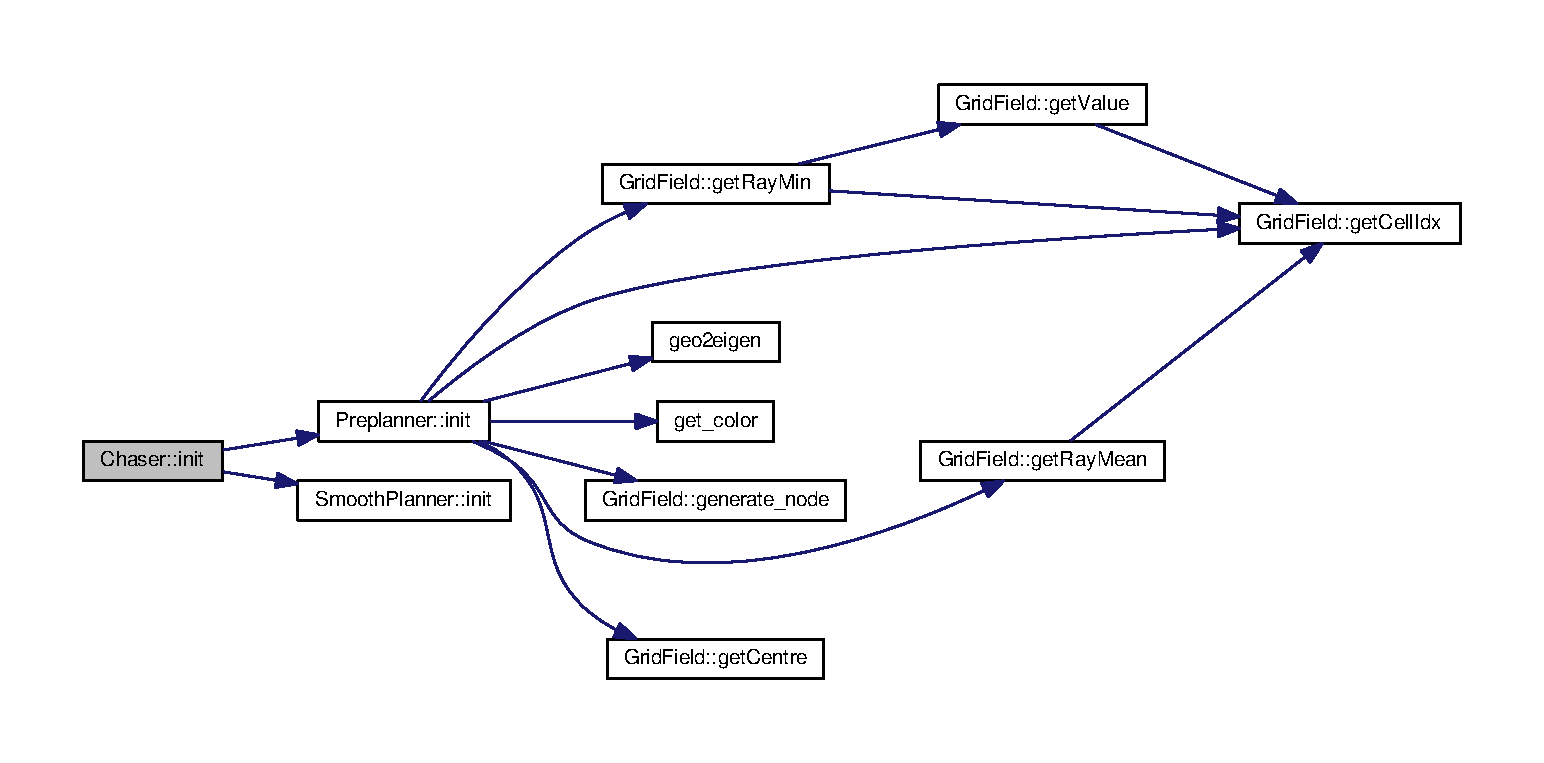
\includegraphics[width=350pt]{class_chaser_a3538485980643e885755608e4297d1f6_cgraph}
\end{center}
\end{figure}


\index{Chaser@{Chaser}!session@{session}}
\index{session@{session}!Chaser@{Chaser}}
\subsubsection[{\texorpdfstring{session(double t)}{session(double t)}}]{\setlength{\rightskip}{0pt plus 5cm}void Chaser\+::session (
\begin{DoxyParamCaption}
\item[{double}]{t}
\end{DoxyParamCaption}
)}\hypertarget{class_chaser_a7d736728bb5327acf0d334d7d4b1b844}{}\label{class_chaser_a7d736728bb5327acf0d334d7d4b1b844}


Definition at line 71 of file Chaser.\+cpp.



Here is the call graph for this function\+:
\nopagebreak
\begin{figure}[H]
\begin{center}
\leavevmode
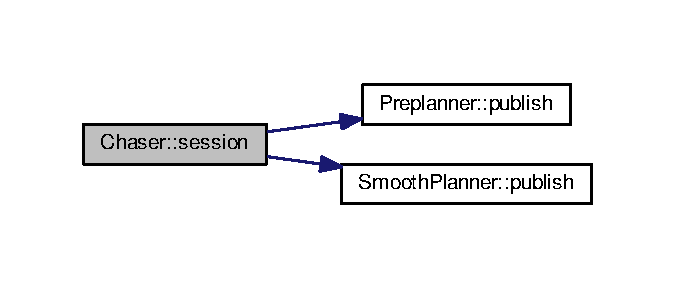
\includegraphics[width=324pt]{class_chaser_a7d736728bb5327acf0d334d7d4b1b844_cgraph}
\end{center}
\end{figure}




\subsection{Member Data Documentation}
\index{Chaser@{Chaser}!is\+\_\+complete\+\_\+chasing\+\_\+path@{is\+\_\+complete\+\_\+chasing\+\_\+path}}
\index{is\+\_\+complete\+\_\+chasing\+\_\+path@{is\+\_\+complete\+\_\+chasing\+\_\+path}!Chaser@{Chaser}}
\subsubsection[{\texorpdfstring{is\+\_\+complete\+\_\+chasing\+\_\+path}{is_complete_chasing_path}}]{\setlength{\rightskip}{0pt plus 5cm}bool Chaser\+::is\+\_\+complete\+\_\+chasing\+\_\+path}\hypertarget{class_chaser_a53af032471ad6bdc828c4eae78085813}{}\label{class_chaser_a53af032471ad6bdc828c4eae78085813}


Definition at line 18 of file Chaser.\+h.

\index{Chaser@{Chaser}!is\+\_\+log@{is\+\_\+log}}
\index{is\+\_\+log@{is\+\_\+log}!Chaser@{Chaser}}
\subsubsection[{\texorpdfstring{is\+\_\+log}{is_log}}]{\setlength{\rightskip}{0pt plus 5cm}bool Chaser\+::is\+\_\+log}\hypertarget{class_chaser_a33b880dd48d1d983001fa93ba1a1184f}{}\label{class_chaser_a33b880dd48d1d983001fa93ba1a1184f}


Definition at line 19 of file Chaser.\+h.

\index{Chaser@{Chaser}!log\+\_\+dir@{log\+\_\+dir}}
\index{log\+\_\+dir@{log\+\_\+dir}!Chaser@{Chaser}}
\subsubsection[{\texorpdfstring{log\+\_\+dir}{log_dir}}]{\setlength{\rightskip}{0pt plus 5cm}string Chaser\+::log\+\_\+dir}\hypertarget{class_chaser_a9d9ad4c7ca00bcda38d2bc809f3e7654}{}\label{class_chaser_a9d9ad4c7ca00bcda38d2bc809f3e7654}


Definition at line 20 of file Chaser.\+h.



The documentation for this class was generated from the following files\+:\begin{DoxyCompactItemize}
\item 
include/auto\+\_\+chaser/\hyperlink{_chaser_8h}{Chaser.\+h}\item 
src/auto\+\_\+chaser/\hyperlink{_chaser_8cpp}{Chaser.\+cpp}\end{DoxyCompactItemize}

\hypertarget{struct_field_params}{}\section{Field\+Params Struct Reference}
\label{struct_field_params}\index{Field\+Params@{Field\+Params}}


{\ttfamily \#include $<$Common.\+h$>$}

\subsection*{Public Attributes}
\begin{DoxyCompactItemize}
\item 
double \hyperlink{struct_field_params_ae702824fca4d3a4b4bbf4ac90084e3a7}{x0}
\item 
double \hyperlink{struct_field_params_ae9d400dadcfaaff44706adae06664c83}{y0}
\item 
double \hyperlink{struct_field_params_a51178f64cc93a37d6d8f774228c24a0f}{z0}
\item 
double \hyperlink{struct_field_params_a9738077907a76512e49cb284ee3f1949}{lx}
\item 
double \hyperlink{struct_field_params_afb39ded77b5714992e9b2f8c5d735d30}{ly}
\item 
double \hyperlink{struct_field_params_ae7532b58aed59f5b47233e57b67acc1a}{lz}
\item 
double \hyperlink{struct_field_params_a520406c76b3abf392401626bc2161370}{resolution}
\item 
double \hyperlink{struct_field_params_ae6eabaa6e593c9dbac48b2f96bea80ec}{ray\+\_\+stride\+\_\+res}
\end{DoxyCompactItemize}


\subsection{Detailed Description}


Definition at line 104 of file Common.\+h.



\subsection{Member Data Documentation}
\index{Field\+Params@{Field\+Params}!lx@{lx}}
\index{lx@{lx}!Field\+Params@{Field\+Params}}
\subsubsection[{\texorpdfstring{lx}{lx}}]{\setlength{\rightskip}{0pt plus 5cm}double Field\+Params\+::lx}\hypertarget{struct_field_params_a9738077907a76512e49cb284ee3f1949}{}\label{struct_field_params_a9738077907a76512e49cb284ee3f1949}


Definition at line 106 of file Common.\+h.

\index{Field\+Params@{Field\+Params}!ly@{ly}}
\index{ly@{ly}!Field\+Params@{Field\+Params}}
\subsubsection[{\texorpdfstring{ly}{ly}}]{\setlength{\rightskip}{0pt plus 5cm}double Field\+Params\+::ly}\hypertarget{struct_field_params_afb39ded77b5714992e9b2f8c5d735d30}{}\label{struct_field_params_afb39ded77b5714992e9b2f8c5d735d30}


Definition at line 106 of file Common.\+h.

\index{Field\+Params@{Field\+Params}!lz@{lz}}
\index{lz@{lz}!Field\+Params@{Field\+Params}}
\subsubsection[{\texorpdfstring{lz}{lz}}]{\setlength{\rightskip}{0pt plus 5cm}double Field\+Params\+::lz}\hypertarget{struct_field_params_ae7532b58aed59f5b47233e57b67acc1a}{}\label{struct_field_params_ae7532b58aed59f5b47233e57b67acc1a}


Definition at line 106 of file Common.\+h.

\index{Field\+Params@{Field\+Params}!ray\+\_\+stride\+\_\+res@{ray\+\_\+stride\+\_\+res}}
\index{ray\+\_\+stride\+\_\+res@{ray\+\_\+stride\+\_\+res}!Field\+Params@{Field\+Params}}
\subsubsection[{\texorpdfstring{ray\+\_\+stride\+\_\+res}{ray_stride_res}}]{\setlength{\rightskip}{0pt plus 5cm}double Field\+Params\+::ray\+\_\+stride\+\_\+res}\hypertarget{struct_field_params_ae6eabaa6e593c9dbac48b2f96bea80ec}{}\label{struct_field_params_ae6eabaa6e593c9dbac48b2f96bea80ec}


Definition at line 108 of file Common.\+h.

\index{Field\+Params@{Field\+Params}!resolution@{resolution}}
\index{resolution@{resolution}!Field\+Params@{Field\+Params}}
\subsubsection[{\texorpdfstring{resolution}{resolution}}]{\setlength{\rightskip}{0pt plus 5cm}double Field\+Params\+::resolution}\hypertarget{struct_field_params_a520406c76b3abf392401626bc2161370}{}\label{struct_field_params_a520406c76b3abf392401626bc2161370}


Definition at line 107 of file Common.\+h.

\index{Field\+Params@{Field\+Params}!x0@{x0}}
\index{x0@{x0}!Field\+Params@{Field\+Params}}
\subsubsection[{\texorpdfstring{x0}{x0}}]{\setlength{\rightskip}{0pt plus 5cm}double Field\+Params\+::x0}\hypertarget{struct_field_params_ae702824fca4d3a4b4bbf4ac90084e3a7}{}\label{struct_field_params_ae702824fca4d3a4b4bbf4ac90084e3a7}


Definition at line 105 of file Common.\+h.

\index{Field\+Params@{Field\+Params}!y0@{y0}}
\index{y0@{y0}!Field\+Params@{Field\+Params}}
\subsubsection[{\texorpdfstring{y0}{y0}}]{\setlength{\rightskip}{0pt plus 5cm}double Field\+Params\+::y0}\hypertarget{struct_field_params_ae9d400dadcfaaff44706adae06664c83}{}\label{struct_field_params_ae9d400dadcfaaff44706adae06664c83}


Definition at line 105 of file Common.\+h.

\index{Field\+Params@{Field\+Params}!z0@{z0}}
\index{z0@{z0}!Field\+Params@{Field\+Params}}
\subsubsection[{\texorpdfstring{z0}{z0}}]{\setlength{\rightskip}{0pt plus 5cm}double Field\+Params\+::z0}\hypertarget{struct_field_params_a51178f64cc93a37d6d8f774228c24a0f}{}\label{struct_field_params_a51178f64cc93a37d6d8f774228c24a0f}


Definition at line 105 of file Common.\+h.



The documentation for this struct was generated from the following file\+:\begin{DoxyCompactItemize}
\item 
include/auto\+\_\+chaser/\hyperlink{_common_8h}{Common.\+h}\end{DoxyCompactItemize}

\hypertarget{struct_grid_field}{}\section{Grid\+Field Struct Reference}
\label{struct_grid_field}\index{Grid\+Field@{Grid\+Field}}


{\ttfamily \#include $<$Common.\+h$>$}



Collaboration diagram for Grid\+Field\+:
\nopagebreak
\begin{figure}[H]
\begin{center}
\leavevmode
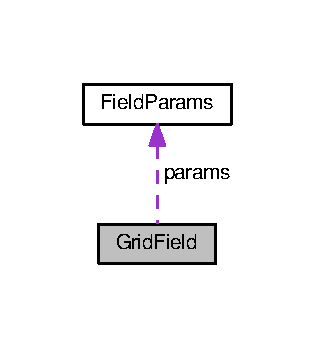
\includegraphics[width=152pt]{struct_grid_field__coll__graph}
\end{center}
\end{figure}
\subsection*{Public Member Functions}
\begin{DoxyCompactItemize}
\item 
\hyperlink{struct_grid_field_a1c755284583cf0070cb3dbed9b5fe925}{Grid\+Field} ()
\item 
\hyperlink{struct_grid_field_ad1542bce01b2a0f0a5860e20ced0e24d}{Grid\+Field} (\hyperlink{struct_field_params}{Field\+Params} param)
\item 
vector$<$ \hyperlink{struct_node}{Node}$<$ Point $>$ $>$ \hyperlink{struct_grid_field_acd8fd9f0893ad94aa4f20b4b4d81802a}{generate\+\_\+node} (int prefix)
\item 
void \hyperlink{struct_grid_field_aa50e5e42c9932e52be3d1d9a38ebf28b}{set\+Origin} (Point X0)
\item 
Point \hyperlink{struct_grid_field_ab0d5ba92ad35ab9b7bdd29506b6753de}{get\+Origin} ()
\item 
Point \hyperlink{struct_grid_field_aacd39f9388090694e5c428cc612fd887}{get\+Centre} ()
\item 
Point \hyperlink{struct_grid_field_ab1a81e68d9e761cfb901c726bd9b0518}{get\+Cell\+Pnt} (Vector3i idx)
\item 
float \hyperlink{struct_grid_field_a9b1f94c44fc47953c38b8e2fe815860d}{get\+Value} (Point pnt)
\item 
Vector3i \hyperlink{struct_grid_field_a1a70c2de6239c1b086d01dc89b161b7c}{get\+Cell\+Idx} (Point pnt)
\item 
vector$<$ Vector3i $>$ \hyperlink{struct_grid_field_a7827c27a1d3b08f930c7f828eef14f0d}{get\+Ray\+Idx} (Point pnt1, Point pnt2)
\item 
float \hyperlink{struct_grid_field_af9f5144af2f0cdb99784ea54c42a8516}{get\+Ray\+Min} (Point pnt1, Point pnt2, float clamping\+\_\+val)
\item 
float \hyperlink{struct_grid_field_a3e49ca50129cb18db833bd4168c5d254}{get\+Ray\+Mean} (Point pnt1, Point pnt2)
\item 
void \hyperlink{struct_grid_field_a5f9debacee6e66e30a30ad7e0759ff15}{update\+Cell} (Point pnt, float val)
\item 
void \hyperlink{struct_grid_field_aeec99711fdc1486528b34fddff21c33f}{update\+Cell} (Vector3i idx, float val)
\item 
int \hyperlink{struct_grid_field_ae838908e288e110c7d1d680fadc6b2ba}{get\+Num\+Cell} ()
\end{DoxyCompactItemize}
\subsection*{Public Attributes}
\begin{DoxyCompactItemize}
\item 
\hyperlink{struct_field_params}{Field\+Params} \hyperlink{struct_grid_field_a735e3033049d10f084e74083ae44dd21}{params}
\item 
Vector\+Xf \hyperlink{struct_grid_field_a14f0f8f41ce92d7e5ab4c539ef9bc495}{node\+\_\+xs}
\item 
Vector\+Xf \hyperlink{struct_grid_field_a07e209546d687dd58557871744f7a9a6}{node\+\_\+ys}
\item 
Vector\+Xf \hyperlink{struct_grid_field_ab97e893cedd450d502165bcb7e3ed7ca}{node\+\_\+zs}
\item 
vector$<$ Point $>$ \hyperlink{struct_grid_field_a76901c3a463e8cbe456c8f73bc264380}{pnts\+\_\+list}
\item 
int \hyperlink{struct_grid_field_a7777c8b5bf6db312fcceecdfd012c9ca}{Nx}
\item 
int \hyperlink{struct_grid_field_a4cc2cac3066c31f0e6af9745cf994674}{Ny}
\item 
int \hyperlink{struct_grid_field_ae624c780496411e632ca5581b84a6177}{Nz}
\item 
vector$<$ Point $>$ \hyperlink{struct_grid_field_ad5dc16fb46eef17df3a554f5b5604611}{saved\+\_\+points}
\item 
float $\ast$$\ast$$\ast$ \hyperlink{struct_grid_field_a46802a85d9533d4371d12597f0247c7d}{field\+\_\+vals}
\end{DoxyCompactItemize}


\subsection{Detailed Description}


Definition at line 137 of file Common.\+h.



\subsection{Constructor \& Destructor Documentation}
\index{Grid\+Field@{Grid\+Field}!Grid\+Field@{Grid\+Field}}
\index{Grid\+Field@{Grid\+Field}!Grid\+Field@{Grid\+Field}}
\subsubsection[{\texorpdfstring{Grid\+Field()}{GridField()}}]{\setlength{\rightskip}{0pt plus 5cm}Grid\+Field\+::\+Grid\+Field (
\begin{DoxyParamCaption}
{}
\end{DoxyParamCaption}
)}\hypertarget{struct_grid_field_a1c755284583cf0070cb3dbed9b5fe925}{}\label{struct_grid_field_a1c755284583cf0070cb3dbed9b5fe925}


Definition at line 90 of file Common.\+cpp.

\index{Grid\+Field@{Grid\+Field}!Grid\+Field@{Grid\+Field}}
\index{Grid\+Field@{Grid\+Field}!Grid\+Field@{Grid\+Field}}
\subsubsection[{\texorpdfstring{Grid\+Field(\+Field\+Params param)}{GridField(FieldParams param)}}]{\setlength{\rightskip}{0pt plus 5cm}Grid\+Field\+::\+Grid\+Field (
\begin{DoxyParamCaption}
\item[{{\bf Field\+Params}}]{param}
\end{DoxyParamCaption}
)}\hypertarget{struct_grid_field_ad1542bce01b2a0f0a5860e20ced0e24d}{}\label{struct_grid_field_ad1542bce01b2a0f0a5860e20ced0e24d}


Definition at line 91 of file Common.\+cpp.



\subsection{Member Function Documentation}
\index{Grid\+Field@{Grid\+Field}!generate\+\_\+node@{generate\+\_\+node}}
\index{generate\+\_\+node@{generate\+\_\+node}!Grid\+Field@{Grid\+Field}}
\subsubsection[{\texorpdfstring{generate\+\_\+node(int prefix)}{generate_node(int prefix)}}]{\setlength{\rightskip}{0pt plus 5cm}vector$<$ {\bf Node}$<$ Point $>$ $>$ Grid\+Field\+::generate\+\_\+node (
\begin{DoxyParamCaption}
\item[{int}]{prefix}
\end{DoxyParamCaption}
)}\hypertarget{struct_grid_field_acd8fd9f0893ad94aa4f20b4b4d81802a}{}\label{struct_grid_field_acd8fd9f0893ad94aa4f20b4b4d81802a}


Definition at line 137 of file Common.\+cpp.



Here is the caller graph for this function\+:
\nopagebreak
\begin{figure}[H]
\begin{center}
\leavevmode
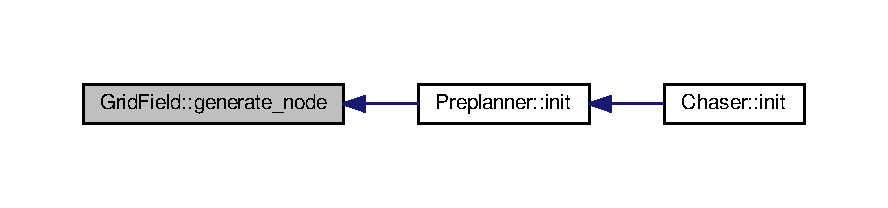
\includegraphics[width=350pt]{struct_grid_field_acd8fd9f0893ad94aa4f20b4b4d81802a_icgraph}
\end{center}
\end{figure}


\index{Grid\+Field@{Grid\+Field}!get\+Cell\+Idx@{get\+Cell\+Idx}}
\index{get\+Cell\+Idx@{get\+Cell\+Idx}!Grid\+Field@{Grid\+Field}}
\subsubsection[{\texorpdfstring{get\+Cell\+Idx(\+Point pnt)}{getCellIdx(Point pnt)}}]{\setlength{\rightskip}{0pt plus 5cm}Vector3i Grid\+Field\+::get\+Cell\+Idx (
\begin{DoxyParamCaption}
\item[{Point}]{pnt}
\end{DoxyParamCaption}
)}\hypertarget{struct_grid_field_a1a70c2de6239c1b086d01dc89b161b7c}{}\label{struct_grid_field_a1a70c2de6239c1b086d01dc89b161b7c}


Definition at line 205 of file Common.\+cpp.



Here is the caller graph for this function\+:
\nopagebreak
\begin{figure}[H]
\begin{center}
\leavevmode
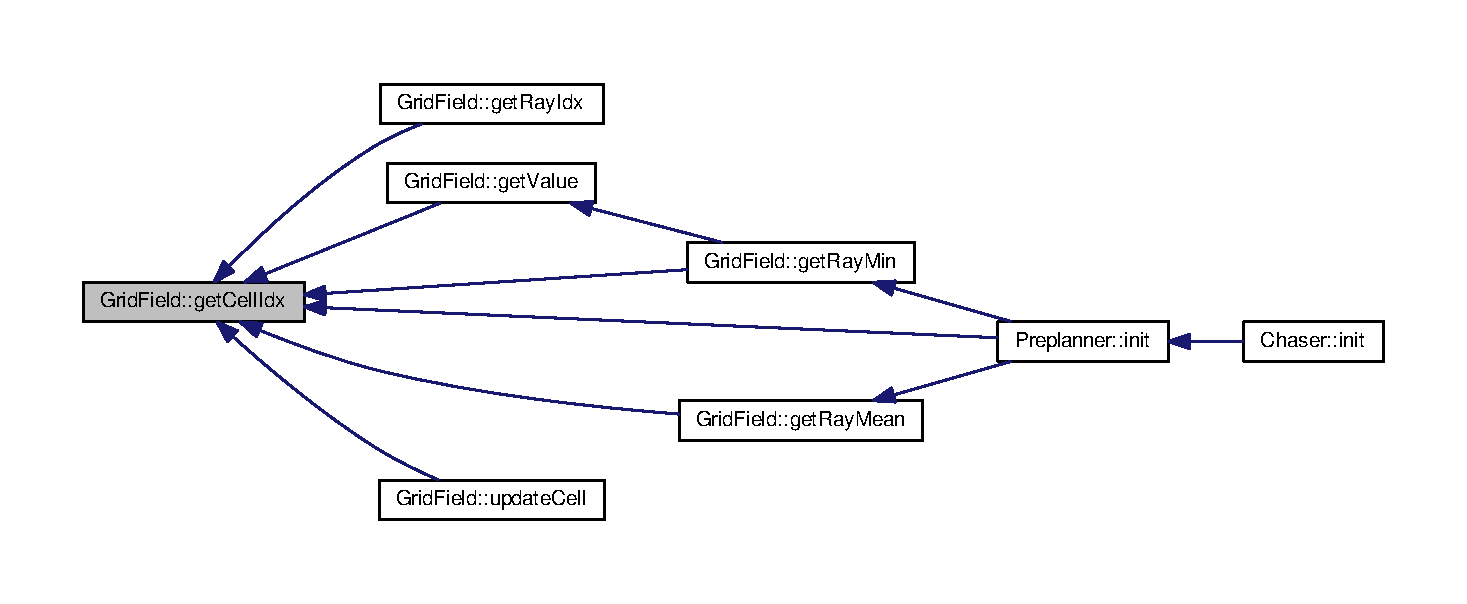
\includegraphics[width=350pt]{struct_grid_field_a1a70c2de6239c1b086d01dc89b161b7c_icgraph}
\end{center}
\end{figure}


\index{Grid\+Field@{Grid\+Field}!get\+Cell\+Pnt@{get\+Cell\+Pnt}}
\index{get\+Cell\+Pnt@{get\+Cell\+Pnt}!Grid\+Field@{Grid\+Field}}
\subsubsection[{\texorpdfstring{get\+Cell\+Pnt(\+Vector3i idx)}{getCellPnt(Vector3i idx)}}]{\setlength{\rightskip}{0pt plus 5cm}Point Grid\+Field\+::get\+Cell\+Pnt (
\begin{DoxyParamCaption}
\item[{Vector3i}]{idx}
\end{DoxyParamCaption}
)}\hypertarget{struct_grid_field_ab1a81e68d9e761cfb901c726bd9b0518}{}\label{struct_grid_field_ab1a81e68d9e761cfb901c726bd9b0518}


Definition at line 184 of file Common.\+cpp.

\index{Grid\+Field@{Grid\+Field}!get\+Centre@{get\+Centre}}
\index{get\+Centre@{get\+Centre}!Grid\+Field@{Grid\+Field}}
\subsubsection[{\texorpdfstring{get\+Centre()}{getCentre()}}]{\setlength{\rightskip}{0pt plus 5cm}Point Grid\+Field\+::get\+Centre (
\begin{DoxyParamCaption}
{}
\end{DoxyParamCaption}
)}\hypertarget{struct_grid_field_aacd39f9388090694e5c428cc612fd887}{}\label{struct_grid_field_aacd39f9388090694e5c428cc612fd887}


Definition at line 176 of file Common.\+cpp.



Here is the caller graph for this function\+:
\nopagebreak
\begin{figure}[H]
\begin{center}
\leavevmode
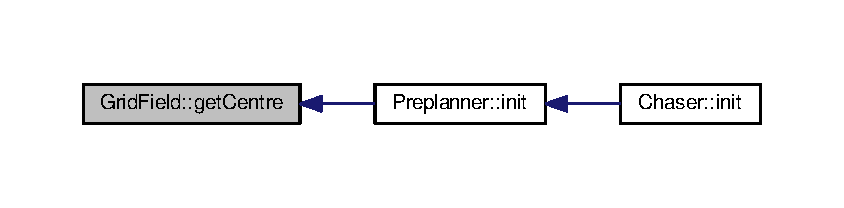
\includegraphics[width=350pt]{struct_grid_field_aacd39f9388090694e5c428cc612fd887_icgraph}
\end{center}
\end{figure}


\index{Grid\+Field@{Grid\+Field}!get\+Num\+Cell@{get\+Num\+Cell}}
\index{get\+Num\+Cell@{get\+Num\+Cell}!Grid\+Field@{Grid\+Field}}
\subsubsection[{\texorpdfstring{get\+Num\+Cell()}{getNumCell()}}]{\setlength{\rightskip}{0pt plus 5cm}int Grid\+Field\+::get\+Num\+Cell (
\begin{DoxyParamCaption}
{}
\end{DoxyParamCaption}
)\hspace{0.3cm}{\ttfamily [inline]}}\hypertarget{struct_grid_field_ae838908e288e110c7d1d680fadc6b2ba}{}\label{struct_grid_field_ae838908e288e110c7d1d680fadc6b2ba}


Definition at line 168 of file Common.\+h.

\index{Grid\+Field@{Grid\+Field}!get\+Origin@{get\+Origin}}
\index{get\+Origin@{get\+Origin}!Grid\+Field@{Grid\+Field}}
\subsubsection[{\texorpdfstring{get\+Origin()}{getOrigin()}}]{\setlength{\rightskip}{0pt plus 5cm}Point Grid\+Field\+::get\+Origin (
\begin{DoxyParamCaption}
{}
\end{DoxyParamCaption}
)}\hypertarget{struct_grid_field_ab0d5ba92ad35ab9b7bdd29506b6753de}{}\label{struct_grid_field_ab0d5ba92ad35ab9b7bdd29506b6753de}


Definition at line 167 of file Common.\+cpp.

\index{Grid\+Field@{Grid\+Field}!get\+Ray\+Idx@{get\+Ray\+Idx}}
\index{get\+Ray\+Idx@{get\+Ray\+Idx}!Grid\+Field@{Grid\+Field}}
\subsubsection[{\texorpdfstring{get\+Ray\+Idx(\+Point pnt1, Point pnt2)}{getRayIdx(Point pnt1, Point pnt2)}}]{\setlength{\rightskip}{0pt plus 5cm}vector$<$ Vector3i $>$ Grid\+Field\+::get\+Ray\+Idx (
\begin{DoxyParamCaption}
\item[{Point}]{pnt1, }
\item[{Point}]{pnt2}
\end{DoxyParamCaption}
)}\hypertarget{struct_grid_field_a7827c27a1d3b08f930c7f828eef14f0d}{}\label{struct_grid_field_a7827c27a1d3b08f930c7f828eef14f0d}


Definition at line 226 of file Common.\+cpp.



Here is the call graph for this function\+:
\nopagebreak
\begin{figure}[H]
\begin{center}
\leavevmode
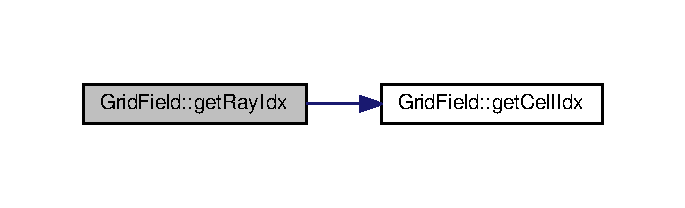
\includegraphics[width=329pt]{struct_grid_field_a7827c27a1d3b08f930c7f828eef14f0d_cgraph}
\end{center}
\end{figure}


\index{Grid\+Field@{Grid\+Field}!get\+Ray\+Mean@{get\+Ray\+Mean}}
\index{get\+Ray\+Mean@{get\+Ray\+Mean}!Grid\+Field@{Grid\+Field}}
\subsubsection[{\texorpdfstring{get\+Ray\+Mean(\+Point pnt1, Point pnt2)}{getRayMean(Point pnt1, Point pnt2)}}]{\setlength{\rightskip}{0pt plus 5cm}float Grid\+Field\+::get\+Ray\+Mean (
\begin{DoxyParamCaption}
\item[{Point}]{pnt1, }
\item[{Point}]{pnt2}
\end{DoxyParamCaption}
)}\hypertarget{struct_grid_field_a3e49ca50129cb18db833bd4168c5d254}{}\label{struct_grid_field_a3e49ca50129cb18db833bd4168c5d254}


Definition at line 303 of file Common.\+cpp.



Here is the call graph for this function\+:
\nopagebreak
\begin{figure}[H]
\begin{center}
\leavevmode
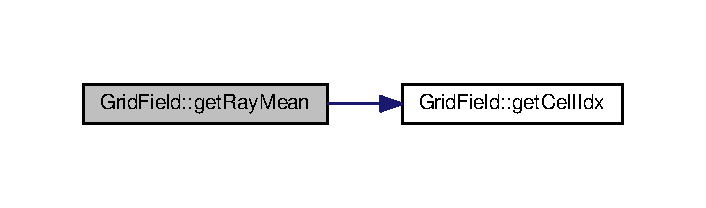
\includegraphics[width=339pt]{struct_grid_field_a3e49ca50129cb18db833bd4168c5d254_cgraph}
\end{center}
\end{figure}




Here is the caller graph for this function\+:
\nopagebreak
\begin{figure}[H]
\begin{center}
\leavevmode
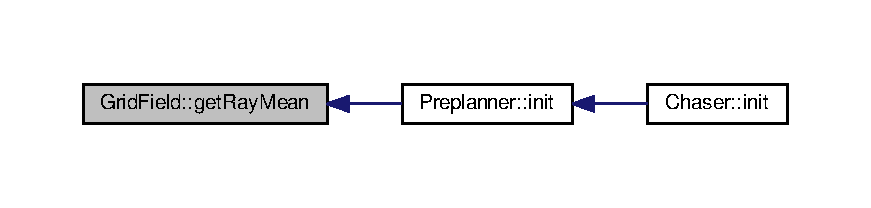
\includegraphics[width=350pt]{struct_grid_field_a3e49ca50129cb18db833bd4168c5d254_icgraph}
\end{center}
\end{figure}


\index{Grid\+Field@{Grid\+Field}!get\+Ray\+Min@{get\+Ray\+Min}}
\index{get\+Ray\+Min@{get\+Ray\+Min}!Grid\+Field@{Grid\+Field}}
\subsubsection[{\texorpdfstring{get\+Ray\+Min(\+Point pnt1, Point pnt2, float clamping\+\_\+val)}{getRayMin(Point pnt1, Point pnt2, float clamping_val)}}]{\setlength{\rightskip}{0pt plus 5cm}float Grid\+Field\+::get\+Ray\+Min (
\begin{DoxyParamCaption}
\item[{Point}]{pnt1, }
\item[{Point}]{pnt2, }
\item[{float}]{clamping\+\_\+val}
\end{DoxyParamCaption}
)}\hypertarget{struct_grid_field_af9f5144af2f0cdb99784ea54c42a8516}{}\label{struct_grid_field_af9f5144af2f0cdb99784ea54c42a8516}


Definition at line 259 of file Common.\+cpp.



Here is the call graph for this function\+:
\nopagebreak
\begin{figure}[H]
\begin{center}
\leavevmode
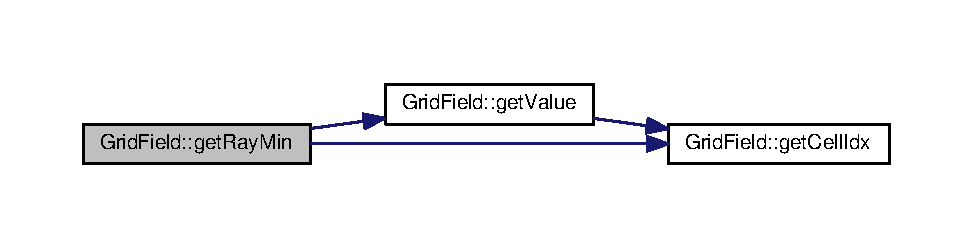
\includegraphics[width=350pt]{struct_grid_field_af9f5144af2f0cdb99784ea54c42a8516_cgraph}
\end{center}
\end{figure}




Here is the caller graph for this function\+:
\nopagebreak
\begin{figure}[H]
\begin{center}
\leavevmode
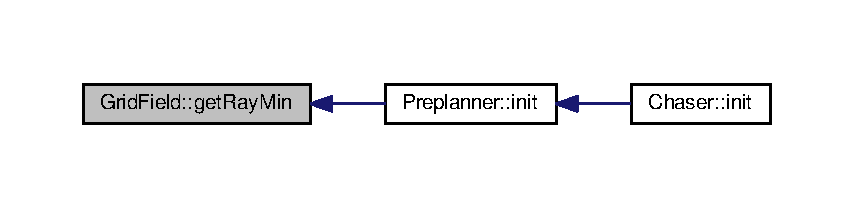
\includegraphics[width=350pt]{struct_grid_field_af9f5144af2f0cdb99784ea54c42a8516_icgraph}
\end{center}
\end{figure}


\index{Grid\+Field@{Grid\+Field}!get\+Value@{get\+Value}}
\index{get\+Value@{get\+Value}!Grid\+Field@{Grid\+Field}}
\subsubsection[{\texorpdfstring{get\+Value(\+Point pnt)}{getValue(Point pnt)}}]{\setlength{\rightskip}{0pt plus 5cm}float Grid\+Field\+::get\+Value (
\begin{DoxyParamCaption}
\item[{Point}]{pnt}
\end{DoxyParamCaption}
)}\hypertarget{struct_grid_field_a9b1f94c44fc47953c38b8e2fe815860d}{}\label{struct_grid_field_a9b1f94c44fc47953c38b8e2fe815860d}


Definition at line 253 of file Common.\+cpp.



Here is the call graph for this function\+:
\nopagebreak
\begin{figure}[H]
\begin{center}
\leavevmode
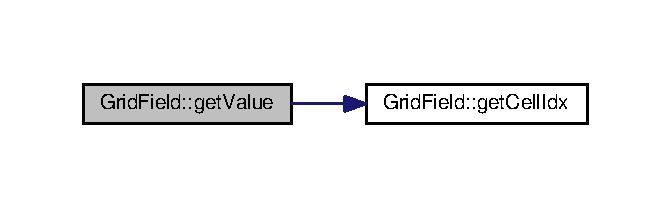
\includegraphics[width=322pt]{struct_grid_field_a9b1f94c44fc47953c38b8e2fe815860d_cgraph}
\end{center}
\end{figure}




Here is the caller graph for this function\+:
\nopagebreak
\begin{figure}[H]
\begin{center}
\leavevmode
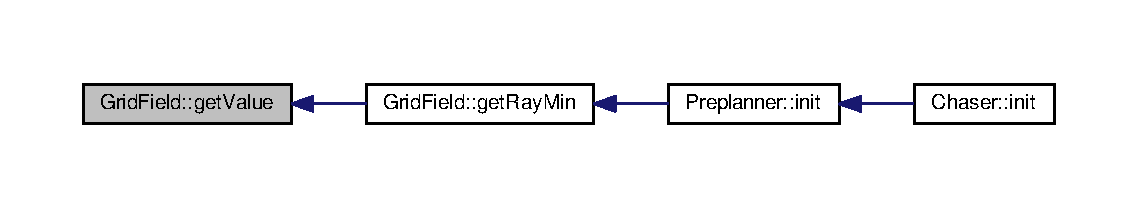
\includegraphics[width=350pt]{struct_grid_field_a9b1f94c44fc47953c38b8e2fe815860d_icgraph}
\end{center}
\end{figure}


\index{Grid\+Field@{Grid\+Field}!set\+Origin@{set\+Origin}}
\index{set\+Origin@{set\+Origin}!Grid\+Field@{Grid\+Field}}
\subsubsection[{\texorpdfstring{set\+Origin(\+Point X0)}{setOrigin(Point X0)}}]{\setlength{\rightskip}{0pt plus 5cm}void Grid\+Field\+::set\+Origin (
\begin{DoxyParamCaption}
\item[{Point}]{X0}
\end{DoxyParamCaption}
)}\hypertarget{struct_grid_field_aa50e5e42c9932e52be3d1d9a38ebf28b}{}\label{struct_grid_field_aa50e5e42c9932e52be3d1d9a38ebf28b}


Definition at line 155 of file Common.\+cpp.

\index{Grid\+Field@{Grid\+Field}!update\+Cell@{update\+Cell}}
\index{update\+Cell@{update\+Cell}!Grid\+Field@{Grid\+Field}}
\subsubsection[{\texorpdfstring{update\+Cell(\+Point pnt, float val)}{updateCell(Point pnt, float val)}}]{\setlength{\rightskip}{0pt plus 5cm}void Grid\+Field\+::update\+Cell (
\begin{DoxyParamCaption}
\item[{Point}]{pnt, }
\item[{float}]{val}
\end{DoxyParamCaption}
)}\hypertarget{struct_grid_field_a5f9debacee6e66e30a30ad7e0759ff15}{}\label{struct_grid_field_a5f9debacee6e66e30a30ad7e0759ff15}


Definition at line 347 of file Common.\+cpp.



Here is the call graph for this function\+:
\nopagebreak
\begin{figure}[H]
\begin{center}
\leavevmode
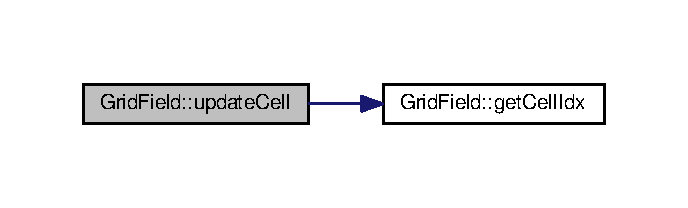
\includegraphics[width=330pt]{struct_grid_field_a5f9debacee6e66e30a30ad7e0759ff15_cgraph}
\end{center}
\end{figure}


\index{Grid\+Field@{Grid\+Field}!update\+Cell@{update\+Cell}}
\index{update\+Cell@{update\+Cell}!Grid\+Field@{Grid\+Field}}
\subsubsection[{\texorpdfstring{update\+Cell(\+Vector3i idx, float val)}{updateCell(Vector3i idx, float val)}}]{\setlength{\rightskip}{0pt plus 5cm}void Grid\+Field\+::update\+Cell (
\begin{DoxyParamCaption}
\item[{Vector3i}]{idx, }
\item[{float}]{val}
\end{DoxyParamCaption}
)}\hypertarget{struct_grid_field_aeec99711fdc1486528b34fddff21c33f}{}\label{struct_grid_field_aeec99711fdc1486528b34fddff21c33f}


Definition at line 356 of file Common.\+cpp.



\subsection{Member Data Documentation}
\index{Grid\+Field@{Grid\+Field}!field\+\_\+vals@{field\+\_\+vals}}
\index{field\+\_\+vals@{field\+\_\+vals}!Grid\+Field@{Grid\+Field}}
\subsubsection[{\texorpdfstring{field\+\_\+vals}{field_vals}}]{\setlength{\rightskip}{0pt plus 5cm}float$\ast$$\ast$$\ast$ Grid\+Field\+::field\+\_\+vals}\hypertarget{struct_grid_field_a46802a85d9533d4371d12597f0247c7d}{}\label{struct_grid_field_a46802a85d9533d4371d12597f0247c7d}


Definition at line 143 of file Common.\+h.

\index{Grid\+Field@{Grid\+Field}!node\+\_\+xs@{node\+\_\+xs}}
\index{node\+\_\+xs@{node\+\_\+xs}!Grid\+Field@{Grid\+Field}}
\subsubsection[{\texorpdfstring{node\+\_\+xs}{node_xs}}]{\setlength{\rightskip}{0pt plus 5cm}Vector\+Xf Grid\+Field\+::node\+\_\+xs}\hypertarget{struct_grid_field_a14f0f8f41ce92d7e5ab4c539ef9bc495}{}\label{struct_grid_field_a14f0f8f41ce92d7e5ab4c539ef9bc495}


Definition at line 139 of file Common.\+h.

\index{Grid\+Field@{Grid\+Field}!node\+\_\+ys@{node\+\_\+ys}}
\index{node\+\_\+ys@{node\+\_\+ys}!Grid\+Field@{Grid\+Field}}
\subsubsection[{\texorpdfstring{node\+\_\+ys}{node_ys}}]{\setlength{\rightskip}{0pt plus 5cm}Vector\+Xf Grid\+Field\+::node\+\_\+ys}\hypertarget{struct_grid_field_a07e209546d687dd58557871744f7a9a6}{}\label{struct_grid_field_a07e209546d687dd58557871744f7a9a6}


Definition at line 139 of file Common.\+h.

\index{Grid\+Field@{Grid\+Field}!node\+\_\+zs@{node\+\_\+zs}}
\index{node\+\_\+zs@{node\+\_\+zs}!Grid\+Field@{Grid\+Field}}
\subsubsection[{\texorpdfstring{node\+\_\+zs}{node_zs}}]{\setlength{\rightskip}{0pt plus 5cm}Vector\+Xf Grid\+Field\+::node\+\_\+zs}\hypertarget{struct_grid_field_ab97e893cedd450d502165bcb7e3ed7ca}{}\label{struct_grid_field_ab97e893cedd450d502165bcb7e3ed7ca}


Definition at line 139 of file Common.\+h.

\index{Grid\+Field@{Grid\+Field}!Nx@{Nx}}
\index{Nx@{Nx}!Grid\+Field@{Grid\+Field}}
\subsubsection[{\texorpdfstring{Nx}{Nx}}]{\setlength{\rightskip}{0pt plus 5cm}int Grid\+Field\+::\+Nx}\hypertarget{struct_grid_field_a7777c8b5bf6db312fcceecdfd012c9ca}{}\label{struct_grid_field_a7777c8b5bf6db312fcceecdfd012c9ca}


Definition at line 141 of file Common.\+h.

\index{Grid\+Field@{Grid\+Field}!Ny@{Ny}}
\index{Ny@{Ny}!Grid\+Field@{Grid\+Field}}
\subsubsection[{\texorpdfstring{Ny}{Ny}}]{\setlength{\rightskip}{0pt plus 5cm}int Grid\+Field\+::\+Ny}\hypertarget{struct_grid_field_a4cc2cac3066c31f0e6af9745cf994674}{}\label{struct_grid_field_a4cc2cac3066c31f0e6af9745cf994674}


Definition at line 141 of file Common.\+h.

\index{Grid\+Field@{Grid\+Field}!Nz@{Nz}}
\index{Nz@{Nz}!Grid\+Field@{Grid\+Field}}
\subsubsection[{\texorpdfstring{Nz}{Nz}}]{\setlength{\rightskip}{0pt plus 5cm}int Grid\+Field\+::\+Nz}\hypertarget{struct_grid_field_ae624c780496411e632ca5581b84a6177}{}\label{struct_grid_field_ae624c780496411e632ca5581b84a6177}


Definition at line 141 of file Common.\+h.

\index{Grid\+Field@{Grid\+Field}!params@{params}}
\index{params@{params}!Grid\+Field@{Grid\+Field}}
\subsubsection[{\texorpdfstring{params}{params}}]{\setlength{\rightskip}{0pt plus 5cm}{\bf Field\+Params} Grid\+Field\+::params}\hypertarget{struct_grid_field_a735e3033049d10f084e74083ae44dd21}{}\label{struct_grid_field_a735e3033049d10f084e74083ae44dd21}


Definition at line 138 of file Common.\+h.

\index{Grid\+Field@{Grid\+Field}!pnts\+\_\+list@{pnts\+\_\+list}}
\index{pnts\+\_\+list@{pnts\+\_\+list}!Grid\+Field@{Grid\+Field}}
\subsubsection[{\texorpdfstring{pnts\+\_\+list}{pnts_list}}]{\setlength{\rightskip}{0pt plus 5cm}vector$<$Point$>$ Grid\+Field\+::pnts\+\_\+list}\hypertarget{struct_grid_field_a76901c3a463e8cbe456c8f73bc264380}{}\label{struct_grid_field_a76901c3a463e8cbe456c8f73bc264380}


Definition at line 140 of file Common.\+h.

\index{Grid\+Field@{Grid\+Field}!saved\+\_\+points@{saved\+\_\+points}}
\index{saved\+\_\+points@{saved\+\_\+points}!Grid\+Field@{Grid\+Field}}
\subsubsection[{\texorpdfstring{saved\+\_\+points}{saved_points}}]{\setlength{\rightskip}{0pt plus 5cm}vector$<$Point$>$ Grid\+Field\+::saved\+\_\+points}\hypertarget{struct_grid_field_ad5dc16fb46eef17df3a554f5b5604611}{}\label{struct_grid_field_ad5dc16fb46eef17df3a554f5b5604611}


Definition at line 142 of file Common.\+h.



The documentation for this struct was generated from the following files\+:\begin{DoxyCompactItemize}
\item 
include/auto\+\_\+chaser/\hyperlink{_common_8h}{Common.\+h}\item 
src/auto\+\_\+chaser/\hyperlink{_common_8cpp}{Common.\+cpp}\end{DoxyCompactItemize}

\hypertarget{class_ui_1_1_main_window}{}\section{Ui\+:\+:Main\+Window Class Reference}
\label{class_ui_1_1_main_window}\index{Ui\+::\+Main\+Window@{Ui\+::\+Main\+Window}}


{\ttfamily \#include $<$ui\+\_\+mainwindow.\+h$>$}



Inheritance diagram for Ui\+:\+:Main\+Window\+:\nopagebreak
\begin{figure}[H]
\begin{center}
\leavevmode
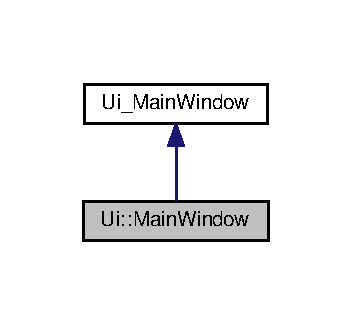
\includegraphics[width=169pt]{class_ui_1_1_main_window__inherit__graph}
\end{center}
\end{figure}


Collaboration diagram for Ui\+:\+:Main\+Window\+:\nopagebreak
\begin{figure}[H]
\begin{center}
\leavevmode
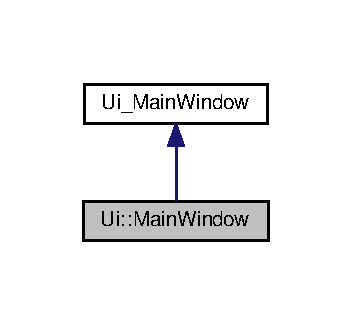
\includegraphics[width=169pt]{class_ui_1_1_main_window__coll__graph}
\end{center}
\end{figure}
\subsection*{Additional Inherited Members}


\subsection{Detailed Description}


The documentation for this class was generated from the following file\+:\begin{DoxyCompactItemize}
\item 
/home/jbs/catkin\+\_\+ws/src/traj\+\_\+gen\+\_\+vis\+\_\+developing/src/build-\/qt\+\_\+ui-\/\+Desktop-\/\+Debug/\hyperlink{ui__mainwindow_8h}{ui\+\_\+mainwindow.\+h}\end{DoxyCompactItemize}

\hypertarget{class_main_window}{}\section{Main\+Window Class Reference}
\label{class_main_window}\index{Main\+Window@{Main\+Window}}


{\ttfamily \#include $<$mainwindow.\+h$>$}



Inheritance diagram for Main\+Window\+:\nopagebreak
\begin{figure}[H]
\begin{center}
\leavevmode
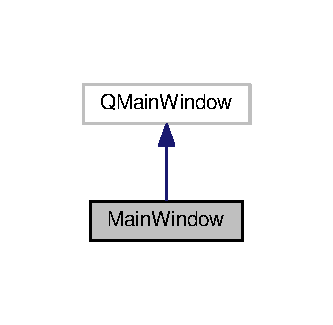
\includegraphics[width=160pt]{class_main_window__inherit__graph}
\end{center}
\end{figure}


Collaboration diagram for Main\+Window\+:
\nopagebreak
\begin{figure}[H]
\begin{center}
\leavevmode
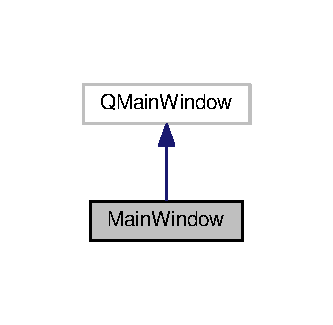
\includegraphics[width=350pt]{class_main_window__coll__graph}
\end{center}
\end{figure}
\subsection*{Public Member Functions}
\begin{DoxyCompactItemize}
\item 
\hyperlink{class_main_window_a6f0a90213d93b861d43c09dd01c52962}{Main\+Window} (\hyperlink{class_q_node}{Q\+Node} $\ast$\hyperlink{class_main_window_ac9d45be6e40fe6917339119e15c1b120}{qnode}, Q\+Widget $\ast$parent=0)
\item 
\hyperlink{class_main_window_ae98d00a93bc118200eeef9f9bba1dba7}{$\sim$\+Main\+Window} ()
\item 
void \hyperlink{class_main_window_a4e20a4a065fbb0e4d3532a45a0a91425}{close\+Event} (Q\+Close\+Event $\ast$event)
\item 
void \hyperlink{class_main_window_a4abba2c52f756524c0f388d0d3e6d6ec}{Read\+Settings} ()
\item 
void \hyperlink{class_main_window_a56a5e4d5e0a022e8c1ecf350d2916ade}{Write\+Settings} ()
\end{DoxyCompactItemize}
\subsection*{Private Slots}
\begin{DoxyCompactItemize}
\item 
void \hyperlink{class_main_window_a996e7b8e246db04a9931ea8c058eedf8}{on\+\_\+push\+Button\+\_\+chaser\+\_\+clicked} ()
\item 
void \hyperlink{class_main_window_a9aebdb686fc8f44bc84454443b094ef7}{on\+\_\+push\+Button\+\_\+ros\+\_\+clicked} ()
\item 
void \hyperlink{class_main_window_a543d311321e5dcb7a42384dd67c6bff4}{on\+\_\+push\+Button\+\_\+waypoint\+\_\+clicked} ()
\item 
void \hyperlink{class_main_window_a3cdeb477328d4aaeac315f62c632a4f2}{on\+\_\+push\+Button\+\_\+trajectory\+\_\+clicked} ()
\item 
void \hyperlink{class_main_window_aec26150ce3a1688a40230b79b088921d}{on\+\_\+push\+Button\+\_\+simulation\+\_\+clicked} ()
\item 
void \hyperlink{class_main_window_a5f2b259d7c85d5d32c1207a34d8b9af4}{on\+\_\+push\+Button\+\_\+save\+\_\+clicked} ()
\item 
void \hyperlink{class_main_window_a9c676468f012e842cd443d8029f8a242}{on\+\_\+push\+Button\+\_\+load\+\_\+clicked} ()
\item 
void \hyperlink{class_main_window_af777763ec745a8eeffe3f9925005fac1}{on\+\_\+push\+Button\+\_\+clear\+\_\+clicked} ()
\item 
void \hyperlink{class_main_window_a41e769472d468772dd3851cbd20ca9fb}{on\+\_\+push\+Button\+\_\+undo\+\_\+clicked} ()
\item 
void \hyperlink{class_main_window_a00ace1276164789fa5383e80ecbf8c6f}{on\+\_\+push\+Button\+\_\+one\+\_\+shot\+\_\+clicked} ()
\item 
void \hyperlink{class_main_window_a4513ffcd68256d01c44fa2602d4c6880}{text\+Edit\+\_\+write} (Q\+String)
\end{DoxyCompactItemize}
\subsection*{Private Attributes}
\begin{DoxyCompactItemize}
\item 
\hyperlink{class_ui_1_1_main_window}{Ui\+::\+Main\+Window} $\ast$ \hyperlink{class_main_window_a35466a70ed47252a0191168126a352a5}{ui}
\item 
\hyperlink{class_q_node}{Q\+Node} $\ast$ \hyperlink{class_main_window_ac9d45be6e40fe6917339119e15c1b120}{qnode}
\end{DoxyCompactItemize}


\subsection{Detailed Description}


\subsection{Constructor \& Destructor Documentation}
\index{Main\+Window@{Main\+Window}!Main\+Window@{Main\+Window}}
\index{Main\+Window@{Main\+Window}!Main\+Window@{Main\+Window}}
\subsubsection[{\texorpdfstring{Main\+Window(\+Q\+Node $\ast$qnode, Q\+Widget $\ast$parent=0)}{MainWindow(QNode *qnode, QWidget *parent=0)}}]{\setlength{\rightskip}{0pt plus 5cm}Main\+Window\+::\+Main\+Window (
\begin{DoxyParamCaption}
\item[{{\bf Q\+Node} $\ast$}]{qnode, }
\item[{Q\+Widget $\ast$}]{parent = {\ttfamily 0}}
\end{DoxyParamCaption}
)\hspace{0.3cm}{\ttfamily [explicit]}}\hypertarget{class_main_window_a6f0a90213d93b861d43c09dd01c52962}{}\label{class_main_window_a6f0a90213d93b861d43c09dd01c52962}

\begin{DoxyCode}
5                                                    :
6     QMainWindow(parent),\hyperlink{class_main_window_ac9d45be6e40fe6917339119e15c1b120}{qnode}(qnode),
7     \hyperlink{class_main_window_a35466a70ed47252a0191168126a352a5}{ui}(\textcolor{keyword}{new} \hyperlink{class_ui_1_1_main_window}{Ui::MainWindow})
8 \{
9     \hyperlink{class_main_window_a35466a70ed47252a0191168126a352a5}{ui}->\hyperlink{class_ui___main_window_acf4a0872c4c77d8f43a2ec66ed849b58}{setupUi}(\textcolor{keyword}{this});
10 
11 
12     \textcolor{comment}{// intial configuration}
13 
14     \textcolor{comment}{// logos}
15     \textcolor{keywordtype}{string} cd = \_\_FILE\_\_;
16     cd.erase(cd.end()-14,cd.end());
17     cout<<\textcolor{stringliteral}{"current directory: "}<<cd<<endl;
18 
19     QPixmap pix\_larr((cd + \textcolor{stringliteral}{"/resources/LARR.jpg"}).c\_str());
20     \textcolor{keywordtype}{int} w = \hyperlink{class_main_window_a35466a70ed47252a0191168126a352a5}{ui}->\hyperlink{class_ui___main_window_a32587f1e879f5b685d375d2daa20f7a6}{label\_larr}->width();
21     \textcolor{keywordtype}{int} h = \hyperlink{class_main_window_a35466a70ed47252a0191168126a352a5}{ui}->\hyperlink{class_ui___main_window_a32587f1e879f5b685d375d2daa20f7a6}{label\_larr}->height();
22     \hyperlink{class_main_window_a35466a70ed47252a0191168126a352a5}{ui}->\hyperlink{class_ui___main_window_a32587f1e879f5b685d375d2daa20f7a6}{label\_larr}->setPixmap(pix\_larr.scaled(w,h,Qt::KeepAspectRatio));
23 
24     QPixmap pix\_larr2((cd +\textcolor{stringliteral}{"/resources/maxresdefault.jpg"}).c\_str());
25     \textcolor{keywordtype}{int} w2 = \hyperlink{class_main_window_a35466a70ed47252a0191168126a352a5}{ui}->\hyperlink{class_ui___main_window_a06fc1a01ac3ba3d4d1f75a0e8ab06684}{label\_larr2}->width();
26     \textcolor{keywordtype}{int} h2 = \hyperlink{class_main_window_a35466a70ed47252a0191168126a352a5}{ui}->\hyperlink{class_ui___main_window_a06fc1a01ac3ba3d4d1f75a0e8ab06684}{label\_larr2}->height();
27     \hyperlink{class_main_window_a35466a70ed47252a0191168126a352a5}{ui}->\hyperlink{class_ui___main_window_a06fc1a01ac3ba3d4d1f75a0e8ab06684}{label\_larr2}->setPixmap(pix\_larr2.scaled(w2,h2,Qt::KeepAspectRatio));
28 
29     \textcolor{comment}{// checkable }
30     \hyperlink{class_main_window_a35466a70ed47252a0191168126a352a5}{ui}->\hyperlink{class_ui___main_window_afd109ead0ad1ae7ae67ad1df803c9c38}{pushButton\_simulation}->setStyleSheet(\textcolor{stringliteral}{"QPushButton:checked\{background-color:
       rgba(100, 20, 20,50); \}"});
31     
32     QObject::connect(qnode, SIGNAL(rosShutdown()), \textcolor{keyword}{this}, SLOT(close()));
33     QObject::connect(qnode,SIGNAL(writeOnBoard(QString)),\textcolor{keyword}{this},SLOT(
      \hyperlink{class_main_window_a4513ffcd68256d01c44fa2602d4c6880}{textEdit\_write}(QString)));
34 
35     \textcolor{comment}{// load settings }
36     \hyperlink{class_main_window_a4abba2c52f756524c0f388d0d3e6d6ec}{ReadSettings}();
37 
38 \}
\end{DoxyCode}
\index{Main\+Window@{Main\+Window}!````~Main\+Window@{$\sim$\+Main\+Window}}
\index{````~Main\+Window@{$\sim$\+Main\+Window}!Main\+Window@{Main\+Window}}
\subsubsection[{\texorpdfstring{$\sim$\+Main\+Window()}{~MainWindow()}}]{\setlength{\rightskip}{0pt plus 5cm}Main\+Window\+::$\sim$\+Main\+Window (
\begin{DoxyParamCaption}
{}
\end{DoxyParamCaption}
)}\hypertarget{class_main_window_ae98d00a93bc118200eeef9f9bba1dba7}{}\label{class_main_window_ae98d00a93bc118200eeef9f9bba1dba7}

\begin{DoxyCode}
41 \{
42     \textcolor{keyword}{delete} \hyperlink{class_main_window_a35466a70ed47252a0191168126a352a5}{ui};
43 \}
\end{DoxyCode}


\subsection{Member Function Documentation}
\index{Main\+Window@{Main\+Window}!close\+Event@{close\+Event}}
\index{close\+Event@{close\+Event}!Main\+Window@{Main\+Window}}
\subsubsection[{\texorpdfstring{close\+Event(\+Q\+Close\+Event $\ast$event)}{closeEvent(QCloseEvent *event)}}]{\setlength{\rightskip}{0pt plus 5cm}void Main\+Window\+::close\+Event (
\begin{DoxyParamCaption}
\item[{Q\+Close\+Event $\ast$}]{event}
\end{DoxyParamCaption}
)}\hypertarget{class_main_window_a4e20a4a065fbb0e4d3532a45a0a91425}{}\label{class_main_window_a4e20a4a065fbb0e4d3532a45a0a91425}

\begin{DoxyCode}
234                                              \{
235 
236         \hyperlink{class_main_window_ac9d45be6e40fe6917339119e15c1b120}{qnode}->\hyperlink{class_q_node_a770568addece696138f515d38408ff5c}{shutdown}();
237         \hyperlink{class_main_window_a56a5e4d5e0a022e8c1ecf350d2916ade}{WriteSettings}();
238         QMainWindow::closeEvent(event);
239 \}
\end{DoxyCode}
\index{Main\+Window@{Main\+Window}!on\+\_\+push\+Button\+\_\+chaser\+\_\+clicked@{on\+\_\+push\+Button\+\_\+chaser\+\_\+clicked}}
\index{on\+\_\+push\+Button\+\_\+chaser\+\_\+clicked@{on\+\_\+push\+Button\+\_\+chaser\+\_\+clicked}!Main\+Window@{Main\+Window}}
\subsubsection[{\texorpdfstring{on\+\_\+push\+Button\+\_\+chaser\+\_\+clicked}{on_pushButton_chaser_clicked}}]{\setlength{\rightskip}{0pt plus 5cm}void Main\+Window\+::on\+\_\+push\+Button\+\_\+chaser\+\_\+clicked (
\begin{DoxyParamCaption}
{}
\end{DoxyParamCaption}
)\hspace{0.3cm}{\ttfamily [private]}, {\ttfamily [slot]}}\hypertarget{class_main_window_a996e7b8e246db04a9931ea8c058eedf8}{}\label{class_main_window_a996e7b8e246db04a9931ea8c058eedf8}

\begin{DoxyCode}
70                                              \{
71 
72     \textcolor{keywordflow}{if}(\hyperlink{class_main_window_a35466a70ed47252a0191168126a352a5}{ui}->\hyperlink{class_ui___main_window_a9e8499b7c9a9717499abde993da72ed5}{pushButton\_chaser}->isChecked())\{      
73         \hyperlink{class_main_window_ac9d45be6e40fe6917339119e15c1b120}{qnode}->\hyperlink{class_q_node_ad2d828488fb632a008c7d3ee0e1d1fa2}{chaser\_wrapper}.\hyperlink{class_wrapper_a8cddd5ffbaeb5ab0b5d8d8d0c74f810f}{objects\_handler}.
      \hyperlink{class_objects_handler_acaefe98eb412d4c32cda2bf0bd602ae7}{is\_insert\_permit} = \textcolor{keyword}{true};  
74         \hyperlink{class_main_window_a35466a70ed47252a0191168126a352a5}{ui}->\hyperlink{class_ui___main_window_af13441b9fd874f1aeb2ec5cefaeb0bce}{textEdit\_board}->append(\textcolor{stringliteral}{"please select chaser init pose: /chaser\_init\_pose"});
75     \}\textcolor{keywordflow}{else}\{
76         \hyperlink{class_main_window_a35466a70ed47252a0191168126a352a5}{ui}->\hyperlink{class_ui___main_window_af13441b9fd874f1aeb2ec5cefaeb0bce}{textEdit\_board}->append(\textcolor{stringliteral}{"finishing chaser spawning selection"});
77         \hyperlink{class_main_window_ac9d45be6e40fe6917339119e15c1b120}{qnode}->\hyperlink{class_q_node_ad2d828488fb632a008c7d3ee0e1d1fa2}{chaser\_wrapper}.\hyperlink{class_wrapper_a8cddd5ffbaeb5ab0b5d8d8d0c74f810f}{objects\_handler}.
      \hyperlink{class_objects_handler_acaefe98eb412d4c32cda2bf0bd602ae7}{is\_insert\_permit} = \textcolor{keyword}{false};  
78 
79     \}
80 
81 \}
\end{DoxyCode}
\index{Main\+Window@{Main\+Window}!on\+\_\+push\+Button\+\_\+clear\+\_\+clicked@{on\+\_\+push\+Button\+\_\+clear\+\_\+clicked}}
\index{on\+\_\+push\+Button\+\_\+clear\+\_\+clicked@{on\+\_\+push\+Button\+\_\+clear\+\_\+clicked}!Main\+Window@{Main\+Window}}
\subsubsection[{\texorpdfstring{on\+\_\+push\+Button\+\_\+clear\+\_\+clicked}{on_pushButton_clear_clicked}}]{\setlength{\rightskip}{0pt plus 5cm}void Main\+Window\+::on\+\_\+push\+Button\+\_\+clear\+\_\+clicked (
\begin{DoxyParamCaption}
{}
\end{DoxyParamCaption}
)\hspace{0.3cm}{\ttfamily [private]}, {\ttfamily [slot]}}\hypertarget{class_main_window_af777763ec745a8eeffe3f9925005fac1}{}\label{class_main_window_af777763ec745a8eeffe3f9925005fac1}

\begin{DoxyCode}
181 \{
182     \hyperlink{class_main_window_ac9d45be6e40fe6917339119e15c1b120}{qnode}->\hyperlink{class_q_node_adc66765125dfd755d5e7f0c0eb6e6395}{target\_manager}.\hyperlink{class_target_manager_a13242c4a8b96b97cfeddea19aabc1181}{clear\_waypoint}();
183 \}
\end{DoxyCode}
\index{Main\+Window@{Main\+Window}!on\+\_\+push\+Button\+\_\+load\+\_\+clicked@{on\+\_\+push\+Button\+\_\+load\+\_\+clicked}}
\index{on\+\_\+push\+Button\+\_\+load\+\_\+clicked@{on\+\_\+push\+Button\+\_\+load\+\_\+clicked}!Main\+Window@{Main\+Window}}
\subsubsection[{\texorpdfstring{on\+\_\+push\+Button\+\_\+load\+\_\+clicked}{on_pushButton_load_clicked}}]{\setlength{\rightskip}{0pt plus 5cm}void Main\+Window\+::on\+\_\+push\+Button\+\_\+load\+\_\+clicked (
\begin{DoxyParamCaption}
{}
\end{DoxyParamCaption}
)\hspace{0.3cm}{\ttfamily [private]}, {\ttfamily [slot]}}\hypertarget{class_main_window_a9c676468f012e842cd443d8029f8a242}{}\label{class_main_window_a9c676468f012e842cd443d8029f8a242}

\begin{DoxyCode}
137 \{
138     \textcolor{comment}{// file read : queue wil be filled with these}
139 
140     \textcolor{keywordtype}{string} filename = \hyperlink{class_main_window_a35466a70ed47252a0191168126a352a5}{ui}->\hyperlink{class_ui___main_window_a4a75bfb754049f89fccef822cad712d6}{lineEdit\_target\_trajectory}->text().toStdString();
141     std::ifstream infile;
142     infile.open(filename);
143     \textcolor{keywordflow}{if}(infile.is\_open())
144         \hyperlink{class_main_window_a35466a70ed47252a0191168126a352a5}{ui}->\hyperlink{class_ui___main_window_af13441b9fd874f1aeb2ec5cefaeb0bce}{textEdit\_board}->append(QString(\textcolor{stringliteral}{"pnts reading.."}));
145     \textcolor{keywordflow}{else}
146     \{
147         \hyperlink{class_main_window_a35466a70ed47252a0191168126a352a5}{ui}->\hyperlink{class_ui___main_window_af13441b9fd874f1aeb2ec5cefaeb0bce}{textEdit\_board}->append(QString(\textcolor{stringliteral}{"could not open file."}));
148         \textcolor{keywordflow}{return};
149     \}
150 
151     std::vector<geometry\_msgs::PoseStamped> queue\_replace;
152 
153     \textcolor{keywordflow}{while} (! infile.eof())\{
154         std::string line;
155         getline(infile, line); \textcolor{comment}{// if no delimiter given, new line is that}
156         \textcolor{comment}{// std::cout<<line<<std::endl;}
157         std::stringstream stream(line);
158         std::string val;
159         \textcolor{keywordtype}{int} xyz\_idx = 0;
160         geometry\_msgs::PoseStamped wpnt;
161 
162         \textcolor{keywordflow}{while}(! stream.eof()) \{
163             getline(stream, val, \textcolor{charliteral}{','});
164             \textcolor{keywordflow}{if}(xyz\_idx == 0)
165                 wpnt.pose.position.x = atof(val.c\_str());
166             \textcolor{keywordflow}{else} \textcolor{keywordflow}{if}(xyz\_idx == 1)
167                 wpnt.pose.position.y = atof(val.c\_str());
168             \textcolor{keywordflow}{else}
169                 wpnt.pose.position.z = atof(val.c\_str());
170             xyz\_idx ++;
171         \}
172         queue\_replace.push\_back(wpnt);
173         \textcolor{comment}{// std::cout<< wpnt.pose.position.x <<" , "<< wpnt.pose.position.y <<" ,
       "<<wpnt.pose.position.z<<std::endl;}
174     \}
175 
176     queue\_replace.pop\_back();
177     \hyperlink{class_main_window_ac9d45be6e40fe6917339119e15c1b120}{qnode}->\hyperlink{class_q_node_adc66765125dfd755d5e7f0c0eb6e6395}{target\_manager}.\hyperlink{class_target_manager_a8b96689879cecac3d9109914eb6230ef}{queue\_file\_load}(queue\_replace);
178 \}
\end{DoxyCode}
\index{Main\+Window@{Main\+Window}!on\+\_\+push\+Button\+\_\+one\+\_\+shot\+\_\+clicked@{on\+\_\+push\+Button\+\_\+one\+\_\+shot\+\_\+clicked}}
\index{on\+\_\+push\+Button\+\_\+one\+\_\+shot\+\_\+clicked@{on\+\_\+push\+Button\+\_\+one\+\_\+shot\+\_\+clicked}!Main\+Window@{Main\+Window}}
\subsubsection[{\texorpdfstring{on\+\_\+push\+Button\+\_\+one\+\_\+shot\+\_\+clicked}{on_pushButton_one_shot_clicked}}]{\setlength{\rightskip}{0pt plus 5cm}void Main\+Window\+::on\+\_\+push\+Button\+\_\+one\+\_\+shot\+\_\+clicked (
\begin{DoxyParamCaption}
{}
\end{DoxyParamCaption}
)\hspace{0.3cm}{\ttfamily [private]}, {\ttfamily [slot]}}\hypertarget{class_main_window_a00ace1276164789fa5383e80ecbf8c6f}{}\label{class_main_window_a00ace1276164789fa5383e80ecbf8c6f}

\begin{DoxyCode}
190                                                \{
191     \hyperlink{class_main_window_a35466a70ed47252a0191168126a352a5}{ui}->\hyperlink{class_ui___main_window_af13441b9fd874f1aeb2ec5cefaeb0bce}{textEdit\_board}->append(\textcolor{stringliteral}{"one shot simulatoin requested."});
192     \textcolor{keywordtype}{double} tf = atoi(\hyperlink{class_main_window_a35466a70ed47252a0191168126a352a5}{ui}->\hyperlink{class_ui___main_window_afc0d94ce5096c619c413cfae9b62014c}{lineEdit\_tf}->text().toStdString().c\_str());    
193     \textcolor{keywordflow}{if} (\hyperlink{class_main_window_ac9d45be6e40fe6917339119e15c1b120}{qnode}->\hyperlink{class_q_node_a65f0fc9f27f336150f33b53a7c51d80b}{trigger\_one\_shot}(tf))
194         \hyperlink{class_main_window_a35466a70ed47252a0191168126a352a5}{ui}->\hyperlink{class_ui___main_window_af13441b9fd874f1aeb2ec5cefaeb0bce}{textEdit\_board}->append(\textcolor{stringliteral}{"chasing path obtained"});
195     \textcolor{keywordflow}{else} 
196         \hyperlink{class_main_window_a35466a70ed47252a0191168126a352a5}{ui}->\hyperlink{class_ui___main_window_af13441b9fd874f1aeb2ec5cefaeb0bce}{textEdit\_board}->append(\textcolor{stringliteral}{"chasing failed"});    
197 \};
\end{DoxyCode}
\index{Main\+Window@{Main\+Window}!on\+\_\+push\+Button\+\_\+ros\+\_\+clicked@{on\+\_\+push\+Button\+\_\+ros\+\_\+clicked}}
\index{on\+\_\+push\+Button\+\_\+ros\+\_\+clicked@{on\+\_\+push\+Button\+\_\+ros\+\_\+clicked}!Main\+Window@{Main\+Window}}
\subsubsection[{\texorpdfstring{on\+\_\+push\+Button\+\_\+ros\+\_\+clicked}{on_pushButton_ros_clicked}}]{\setlength{\rightskip}{0pt plus 5cm}void Main\+Window\+::on\+\_\+push\+Button\+\_\+ros\+\_\+clicked (
\begin{DoxyParamCaption}
{}
\end{DoxyParamCaption}
)\hspace{0.3cm}{\ttfamily [private]}, {\ttfamily [slot]}}\hypertarget{class_main_window_a9aebdb686fc8f44bc84454443b094ef7}{}\label{class_main_window_a9aebdb686fc8f44bc84454443b094ef7}

\begin{DoxyCode}
46 \{
47     \textcolor{keywordflow}{if}(\hyperlink{class_main_window_ac9d45be6e40fe6917339119e15c1b120}{qnode}->\hyperlink{class_q_node_a32d00dbcf15c277e08caabf95af04f6e}{on\_init}())\{
48         \hyperlink{class_main_window_a35466a70ed47252a0191168126a352a5}{ui}->\hyperlink{class_ui___main_window_af13441b9fd874f1aeb2ec5cefaeb0bce}{textEdit\_board}->append(\textcolor{stringliteral}{"ros connected."});
49         \hyperlink{class_main_window_ac9d45be6e40fe6917339119e15c1b120}{qnode}->\hyperlink{class_q_node_a98b08e7704b00df8648f8c08dffe950c}{is\_connected} = \textcolor{keyword}{true};
50 
51     \}\textcolor{keywordflow}{else}\{
52         \hyperlink{class_main_window_a35466a70ed47252a0191168126a352a5}{ui}->\hyperlink{class_ui___main_window_af13441b9fd874f1aeb2ec5cefaeb0bce}{textEdit\_board}->append(\textcolor{stringliteral}{"failed. retry"});
53     \}
54 \}
\end{DoxyCode}
\index{Main\+Window@{Main\+Window}!on\+\_\+push\+Button\+\_\+save\+\_\+clicked@{on\+\_\+push\+Button\+\_\+save\+\_\+clicked}}
\index{on\+\_\+push\+Button\+\_\+save\+\_\+clicked@{on\+\_\+push\+Button\+\_\+save\+\_\+clicked}!Main\+Window@{Main\+Window}}
\subsubsection[{\texorpdfstring{on\+\_\+push\+Button\+\_\+save\+\_\+clicked}{on_pushButton_save_clicked}}]{\setlength{\rightskip}{0pt plus 5cm}void Main\+Window\+::on\+\_\+push\+Button\+\_\+save\+\_\+clicked (
\begin{DoxyParamCaption}
{}
\end{DoxyParamCaption}
)\hspace{0.3cm}{\ttfamily [private]}, {\ttfamily [slot]}}\hypertarget{class_main_window_a5f2b259d7c85d5d32c1207a34d8b9af4}{}\label{class_main_window_a5f2b259d7c85d5d32c1207a34d8b9af4}

\begin{DoxyCode}
115 \{
116 
117     \textcolor{comment}{// file write}
118     std::ofstream wnpt\_file;
119     \textcolor{keywordtype}{string} filename = \hyperlink{class_main_window_a35466a70ed47252a0191168126a352a5}{ui}->\hyperlink{class_ui___main_window_a4a75bfb754049f89fccef822cad712d6}{lineEdit\_target\_trajectory}->text().toStdString();
120     wnpt\_file.open(filename);
121 
122     \textcolor{keywordflow}{if}(wnpt\_file.is\_open())\{
123         \textcolor{keywordflow}{for}(\textcolor{keyword}{auto} it = \hyperlink{class_main_window_ac9d45be6e40fe6917339119e15c1b120}{qnode}->\hyperlink{class_q_node_adc66765125dfd755d5e7f0c0eb6e6395}{target\_manager}.\hyperlink{class_target_manager_a0bbcb1981504e3bc587c3a98f41a91e9}{queue}.begin();it<
      \hyperlink{class_main_window_ac9d45be6e40fe6917339119e15c1b120}{qnode}->\hyperlink{class_q_node_adc66765125dfd755d5e7f0c0eb6e6395}{target\_manager}.\hyperlink{class_target_manager_a0bbcb1981504e3bc587c3a98f41a91e9}{queue}.end();it++)\{
124             wnpt\_file<<std::to\_string(it->pose.position.x)<<\textcolor{stringliteral}{","}<<std::to\_string(it->pose.position.y)<<\textcolor{stringliteral}{","}<<
      std::to\_string(it->pose.position.z)<<\textcolor{stringliteral}{"\(\backslash\)n"};
125         \}
126         wnpt\_file.close();
127 
128         
129         \hyperlink{class_main_window_a35466a70ed47252a0191168126a352a5}{ui}->\hyperlink{class_ui___main_window_af13441b9fd874f1aeb2ec5cefaeb0bce}{textEdit\_board}->append(QString((\textcolor{keywordtype}{string}(\textcolor{stringliteral}{"to "}) + 
      \hyperlink{_common_8h_a7770cb36d4f4c6e78ff68516ecb2123c}{GetCurrentWorkingDir}()+\textcolor{stringliteral}{"/"} + filename + \textcolor{keywordtype}{string}(\textcolor{stringliteral}{", written"})).data()));
130 
131     \}\textcolor{keywordflow}{else}
132         \hyperlink{class_main_window_a35466a70ed47252a0191168126a352a5}{ui}->\hyperlink{class_ui___main_window_af13441b9fd874f1aeb2ec5cefaeb0bce}{textEdit\_board}->append(QString(\textcolor{stringliteral}{"file not written."}));
133 
134 \}
\end{DoxyCode}
\index{Main\+Window@{Main\+Window}!on\+\_\+push\+Button\+\_\+simulation\+\_\+clicked@{on\+\_\+push\+Button\+\_\+simulation\+\_\+clicked}}
\index{on\+\_\+push\+Button\+\_\+simulation\+\_\+clicked@{on\+\_\+push\+Button\+\_\+simulation\+\_\+clicked}!Main\+Window@{Main\+Window}}
\subsubsection[{\texorpdfstring{on\+\_\+push\+Button\+\_\+simulation\+\_\+clicked}{on_pushButton_simulation_clicked}}]{\setlength{\rightskip}{0pt plus 5cm}void Main\+Window\+::on\+\_\+push\+Button\+\_\+simulation\+\_\+clicked (
\begin{DoxyParamCaption}
{}
\end{DoxyParamCaption}
)\hspace{0.3cm}{\ttfamily [private]}, {\ttfamily [slot]}}\hypertarget{class_main_window_aec26150ce3a1688a40230b79b088921d}{}\label{class_main_window_aec26150ce3a1688a40230b79b088921d}

\begin{DoxyCode}
94 \{
95     \textcolor{keywordflow}{if}(\hyperlink{class_main_window_a35466a70ed47252a0191168126a352a5}{ui}->\hyperlink{class_ui___main_window_afd109ead0ad1ae7ae67ad1df803c9c38}{pushButton\_simulation}->isChecked())\{ 
96 
97         \textcolor{keywordflow}{if}(\hyperlink{class_main_window_ac9d45be6e40fe6917339119e15c1b120}{qnode}->\hyperlink{class_q_node_ad2d828488fb632a008c7d3ee0e1d1fa2}{chaser\_wrapper}.\hyperlink{class_wrapper_a8cddd5ffbaeb5ab0b5d8d8d0c74f810f}{objects\_handler}.
      \hyperlink{class_objects_handler_a16165ae7c0167ba8d2a0151a8a4fbfd5}{is\_chaser\_spawned} and \hyperlink{class_main_window_ac9d45be6e40fe6917339119e15c1b120}{qnode}->\hyperlink{class_q_node_adc66765125dfd755d5e7f0c0eb6e6395}{target\_manager}.
      \hyperlink{class_target_manager_a507af7ce1ac562510c1b907553a2e596}{is\_path})\{
98             \hyperlink{class_main_window_a35466a70ed47252a0191168126a352a5}{ui}->\hyperlink{class_ui___main_window_af13441b9fd874f1aeb2ec5cefaeb0bce}{textEdit\_board}->append(\textcolor{stringliteral}{"move target.."});
99             \textcolor{comment}{// simulation end time }
100             \hyperlink{class_main_window_ac9d45be6e40fe6917339119e15c1b120}{qnode}->\hyperlink{class_q_node_a7a127726e48aa5bde733d715af7a744c}{simulation\_end\_time} = atof(\hyperlink{class_main_window_a35466a70ed47252a0191168126a352a5}{ui}->
      \hyperlink{class_ui___main_window_afc0d94ce5096c619c413cfae9b62014c}{lineEdit\_tf}->text().toStdString().c\_str());
101             \hyperlink{class_main_window_ac9d45be6e40fe6917339119e15c1b120}{qnode}->\hyperlink{class_q_node_a6ace2d0aa89adecfe699b3f1c3ce0b0f}{is\_in\_session} = \textcolor{keyword}{true};
102             \hyperlink{class_main_window_ac9d45be6e40fe6917339119e15c1b120}{qnode}->\hyperlink{class_q_node_a96e6599c14732ded065ae6a5b004f872}{button\_click\_time} = ros::Time::now();        
103         \}
104         \textcolor{keywordflow}{else}\{
105             \hyperlink{class_main_window_a35466a70ed47252a0191168126a352a5}{ui}->\hyperlink{class_ui___main_window_af13441b9fd874f1aeb2ec5cefaeb0bce}{textEdit\_board}->append(\textcolor{stringliteral}{"target path not obtained or no chaser spawned."});
106         \}
107     \}\textcolor{keywordflow}{else}\{
108         \hyperlink{class_main_window_a35466a70ed47252a0191168126a352a5}{ui}->\hyperlink{class_ui___main_window_af13441b9fd874f1aeb2ec5cefaeb0bce}{textEdit\_board}->append(\textcolor{stringliteral}{"stop target."});
109         \hyperlink{class_main_window_ac9d45be6e40fe6917339119e15c1b120}{qnode}->\hyperlink{class_q_node_a6ace2d0aa89adecfe699b3f1c3ce0b0f}{is\_in\_session} = \textcolor{keyword}{false};
110         \hyperlink{class_main_window_ac9d45be6e40fe6917339119e15c1b120}{qnode}->\hyperlink{class_q_node_a4b5f0a40821fbb176de620cb5a3921f7}{previous\_elapsed} = (ros::Time::now() - \hyperlink{class_main_window_ac9d45be6e40fe6917339119e15c1b120}{qnode}->
      \hyperlink{class_q_node_a96e6599c14732ded065ae6a5b004f872}{button\_click\_time}).toSec() + \hyperlink{class_main_window_ac9d45be6e40fe6917339119e15c1b120}{qnode}->\hyperlink{class_q_node_a4b5f0a40821fbb176de620cb5a3921f7}{previous\_elapsed}; \textcolor{comment}{// total
       elasped time}
111     \}
112 \}
\end{DoxyCode}
\index{Main\+Window@{Main\+Window}!on\+\_\+push\+Button\+\_\+trajectory\+\_\+clicked@{on\+\_\+push\+Button\+\_\+trajectory\+\_\+clicked}}
\index{on\+\_\+push\+Button\+\_\+trajectory\+\_\+clicked@{on\+\_\+push\+Button\+\_\+trajectory\+\_\+clicked}!Main\+Window@{Main\+Window}}
\subsubsection[{\texorpdfstring{on\+\_\+push\+Button\+\_\+trajectory\+\_\+clicked}{on_pushButton_trajectory_clicked}}]{\setlength{\rightskip}{0pt plus 5cm}void Main\+Window\+::on\+\_\+push\+Button\+\_\+trajectory\+\_\+clicked (
\begin{DoxyParamCaption}
{}
\end{DoxyParamCaption}
)\hspace{0.3cm}{\ttfamily [private]}, {\ttfamily [slot]}}\hypertarget{class_main_window_a3cdeb477328d4aaeac315f62c632a4f2}{}\label{class_main_window_a3cdeb477328d4aaeac315f62c632a4f2}

\begin{DoxyCode}
84 \{
85     
86     \textcolor{keywordtype}{double} tf = atof(\hyperlink{class_main_window_a35466a70ed47252a0191168126a352a5}{ui}->\hyperlink{class_ui___main_window_afc0d94ce5096c619c413cfae9b62014c}{lineEdit\_tf}->text().toStdString().c\_str());
87     \textcolor{keywordflow}{if}(\hyperlink{class_main_window_ac9d45be6e40fe6917339119e15c1b120}{qnode}->\hyperlink{class_q_node_adc66765125dfd755d5e7f0c0eb6e6395}{target\_manager}.\hyperlink{class_target_manager_a1c0e48d7a623e8b7caa11c6b1832956b}{global\_path\_generate}(tf))
88         \hyperlink{class_main_window_a4513ffcd68256d01c44fa2602d4c6880}{textEdit\_write}(\textcolor{stringliteral}{"target trajectory obtainted"});
89     \textcolor{keywordflow}{else}
90         \hyperlink{class_main_window_a4513ffcd68256d01c44fa2602d4c6880}{textEdit\_write}(\textcolor{stringliteral}{"target trajectory failed"});    
91 \}
\end{DoxyCode}
\index{Main\+Window@{Main\+Window}!on\+\_\+push\+Button\+\_\+undo\+\_\+clicked@{on\+\_\+push\+Button\+\_\+undo\+\_\+clicked}}
\index{on\+\_\+push\+Button\+\_\+undo\+\_\+clicked@{on\+\_\+push\+Button\+\_\+undo\+\_\+clicked}!Main\+Window@{Main\+Window}}
\subsubsection[{\texorpdfstring{on\+\_\+push\+Button\+\_\+undo\+\_\+clicked}{on_pushButton_undo_clicked}}]{\setlength{\rightskip}{0pt plus 5cm}void Main\+Window\+::on\+\_\+push\+Button\+\_\+undo\+\_\+clicked (
\begin{DoxyParamCaption}
{}
\end{DoxyParamCaption}
)\hspace{0.3cm}{\ttfamily [private]}, {\ttfamily [slot]}}\hypertarget{class_main_window_a41e769472d468772dd3851cbd20ca9fb}{}\label{class_main_window_a41e769472d468772dd3851cbd20ca9fb}

\begin{DoxyCode}
186 \{
187     \hyperlink{class_main_window_ac9d45be6e40fe6917339119e15c1b120}{qnode}->\hyperlink{class_q_node_adc66765125dfd755d5e7f0c0eb6e6395}{target\_manager}.\hyperlink{class_target_manager_af362d78ae6b0cc0a3ea288b2c138f482}{pop\_waypoint}();
188 \};
\end{DoxyCode}
\index{Main\+Window@{Main\+Window}!on\+\_\+push\+Button\+\_\+waypoint\+\_\+clicked@{on\+\_\+push\+Button\+\_\+waypoint\+\_\+clicked}}
\index{on\+\_\+push\+Button\+\_\+waypoint\+\_\+clicked@{on\+\_\+push\+Button\+\_\+waypoint\+\_\+clicked}!Main\+Window@{Main\+Window}}
\subsubsection[{\texorpdfstring{on\+\_\+push\+Button\+\_\+waypoint\+\_\+clicked}{on_pushButton_waypoint_clicked}}]{\setlength{\rightskip}{0pt plus 5cm}void Main\+Window\+::on\+\_\+push\+Button\+\_\+waypoint\+\_\+clicked (
\begin{DoxyParamCaption}
{}
\end{DoxyParamCaption}
)\hspace{0.3cm}{\ttfamily [private]}, {\ttfamily [slot]}}\hypertarget{class_main_window_a543d311321e5dcb7a42384dd67c6bff4}{}\label{class_main_window_a543d311321e5dcb7a42384dd67c6bff4}

\begin{DoxyCode}
57 \{
58     \textcolor{keywordflow}{if}(\hyperlink{class_main_window_a35466a70ed47252a0191168126a352a5}{ui}->\hyperlink{class_ui___main_window_a6b5d7c0f96cdb3276a33746fbcd7e8c7}{pushButton\_waypoint}->isChecked())\{        
59         \hyperlink{class_main_window_a35466a70ed47252a0191168126a352a5}{ui}->\hyperlink{class_ui___main_window_af13441b9fd874f1aeb2ec5cefaeb0bce}{textEdit\_board}->append(\textcolor{stringliteral}{"please select waypoints : /target\_waypoints "});
60         \hyperlink{class_main_window_ac9d45be6e40fe6917339119e15c1b120}{qnode}->\hyperlink{class_q_node_adc66765125dfd755d5e7f0c0eb6e6395}{target\_manager}.\hyperlink{class_target_manager_adf8a01c0942c3aac0445403d8f0f4cce}{is\_insert\_permit} = \textcolor{keyword}{true};
61 
62     \}\textcolor{keywordflow}{else}\{
63 
64         \hyperlink{class_main_window_a35466a70ed47252a0191168126a352a5}{ui}->\hyperlink{class_ui___main_window_af13441b9fd874f1aeb2ec5cefaeb0bce}{textEdit\_board}->append(\textcolor{stringliteral}{"finishing waypoints selection"});
65         \hyperlink{class_main_window_ac9d45be6e40fe6917339119e15c1b120}{qnode}->\hyperlink{class_q_node_adc66765125dfd755d5e7f0c0eb6e6395}{target\_manager}.\hyperlink{class_target_manager_adf8a01c0942c3aac0445403d8f0f4cce}{is\_insert\_permit} = \textcolor{keyword}{false};
66     \}
67 
68 \}
\end{DoxyCode}
\index{Main\+Window@{Main\+Window}!Read\+Settings@{Read\+Settings}}
\index{Read\+Settings@{Read\+Settings}!Main\+Window@{Main\+Window}}
\subsubsection[{\texorpdfstring{Read\+Settings()}{ReadSettings()}}]{\setlength{\rightskip}{0pt plus 5cm}void Main\+Window\+::\+Read\+Settings (
\begin{DoxyParamCaption}
{}
\end{DoxyParamCaption}
)}\hypertarget{class_main_window_a4abba2c52f756524c0f388d0d3e6d6ec}{}\label{class_main_window_a4abba2c52f756524c0f388d0d3e6d6ec}

\begin{DoxyCode}
204                              \{
205     QSettings settings(\textcolor{stringliteral}{"auto\_chaser"}, \hyperlink{class_main_window_ac9d45be6e40fe6917339119e15c1b120}{qnode}->\hyperlink{class_q_node_ac21ae24311df97ac0e15c97179763b0e}{nodeName}().c\_str());
206 
207     \textcolor{comment}{// setting names    }
208     QString filename\_logging = settings.value(\textcolor{stringliteral}{"filename\_logging"},QString(\textcolor{stringliteral}{"path\_saved.txt"})).toString();
209     QString filename\_waypoints = settings.value(\textcolor{stringliteral}{"filename\_waypoints"},QString(\textcolor{stringliteral}{"path\_saved.txt"})).toString();
210     QString simulation\_tf = settings.value(\textcolor{stringliteral}{"tf"}, QString(\textcolor{stringliteral}{"20"})).toString();
211 
212     
213     \textcolor{comment}{// fill with previous settings }
214     \hyperlink{class_main_window_a35466a70ed47252a0191168126a352a5}{ui}->\hyperlink{class_ui___main_window_a7ab71242b81ef9d13f83c16f6328f35d}{lineEdit\_logging\_dir}->setText(filename\_logging);
215     \hyperlink{class_main_window_a35466a70ed47252a0191168126a352a5}{ui}->\hyperlink{class_ui___main_window_afc0d94ce5096c619c413cfae9b62014c}{lineEdit\_tf}->setText(simulation\_tf);
216     \hyperlink{class_main_window_a35466a70ed47252a0191168126a352a5}{ui}->\hyperlink{class_ui___main_window_a4a75bfb754049f89fccef822cad712d6}{lineEdit\_target\_trajectory}->setText(filename\_waypoints);
217     
218 \}
\end{DoxyCode}
\index{Main\+Window@{Main\+Window}!text\+Edit\+\_\+write@{text\+Edit\+\_\+write}}
\index{text\+Edit\+\_\+write@{text\+Edit\+\_\+write}!Main\+Window@{Main\+Window}}
\subsubsection[{\texorpdfstring{text\+Edit\+\_\+write}{textEdit_write}}]{\setlength{\rightskip}{0pt plus 5cm}void Main\+Window\+::text\+Edit\+\_\+write (
\begin{DoxyParamCaption}
\item[{Q\+String}]{line}
\end{DoxyParamCaption}
)\hspace{0.3cm}{\ttfamily [private]}, {\ttfamily [slot]}}\hypertarget{class_main_window_a4513ffcd68256d01c44fa2602d4c6880}{}\label{class_main_window_a4513ffcd68256d01c44fa2602d4c6880}

\begin{DoxyCode}
199                                            \{    
200     \hyperlink{class_main_window_a35466a70ed47252a0191168126a352a5}{ui}->\hyperlink{class_ui___main_window_af13441b9fd874f1aeb2ec5cefaeb0bce}{textEdit\_board}->append(line);
201 \};
\end{DoxyCode}
\index{Main\+Window@{Main\+Window}!Write\+Settings@{Write\+Settings}}
\index{Write\+Settings@{Write\+Settings}!Main\+Window@{Main\+Window}}
\subsubsection[{\texorpdfstring{Write\+Settings()}{WriteSettings()}}]{\setlength{\rightskip}{0pt plus 5cm}void Main\+Window\+::\+Write\+Settings (
\begin{DoxyParamCaption}
{}
\end{DoxyParamCaption}
)}\hypertarget{class_main_window_a56a5e4d5e0a022e8c1ecf350d2916ade}{}\label{class_main_window_a56a5e4d5e0a022e8c1ecf350d2916ade}

\begin{DoxyCode}
220                               \{
221 
222     QSettings settings(\textcolor{stringliteral}{"auto\_chaser"}, \hyperlink{class_main_window_ac9d45be6e40fe6917339119e15c1b120}{qnode}->\hyperlink{class_q_node_ac21ae24311df97ac0e15c97179763b0e}{nodeName}().c\_str());
223     
224     settings.setValue(\textcolor{stringliteral}{"geometry"}, geometry());
225     settings.setValue(\textcolor{stringliteral}{"windowState"}, saveState());
226 
227     settings.setValue(\textcolor{stringliteral}{"filename\_logging"},\hyperlink{class_main_window_a35466a70ed47252a0191168126a352a5}{ui}->\hyperlink{class_ui___main_window_a7ab71242b81ef9d13f83c16f6328f35d}{lineEdit\_logging\_dir}->text());
228     settings.setValue(\textcolor{stringliteral}{"tf"},\hyperlink{class_main_window_a35466a70ed47252a0191168126a352a5}{ui}->\hyperlink{class_ui___main_window_afc0d94ce5096c619c413cfae9b62014c}{lineEdit\_tf}->text());
229     settings.setValue(\textcolor{stringliteral}{"filename\_waypoints"},\hyperlink{class_main_window_a35466a70ed47252a0191168126a352a5}{ui}->\hyperlink{class_ui___main_window_a4a75bfb754049f89fccef822cad712d6}{lineEdit\_target\_trajectory}->text
      ());
230 
231 
232 \}
\end{DoxyCode}


\subsection{Member Data Documentation}
\index{Main\+Window@{Main\+Window}!qnode@{qnode}}
\index{qnode@{qnode}!Main\+Window@{Main\+Window}}
\subsubsection[{\texorpdfstring{qnode}{qnode}}]{\setlength{\rightskip}{0pt plus 5cm}{\bf Q\+Node}$\ast$ Main\+Window\+::qnode\hspace{0.3cm}{\ttfamily [private]}}\hypertarget{class_main_window_ac9d45be6e40fe6917339119e15c1b120}{}\label{class_main_window_ac9d45be6e40fe6917339119e15c1b120}
\index{Main\+Window@{Main\+Window}!ui@{ui}}
\index{ui@{ui}!Main\+Window@{Main\+Window}}
\subsubsection[{\texorpdfstring{ui}{ui}}]{\setlength{\rightskip}{0pt plus 5cm}{\bf Ui\+::\+Main\+Window}$\ast$ Main\+Window\+::ui\hspace{0.3cm}{\ttfamily [private]}}\hypertarget{class_main_window_a35466a70ed47252a0191168126a352a5}{}\label{class_main_window_a35466a70ed47252a0191168126a352a5}


The documentation for this class was generated from the following files\+:\begin{DoxyCompactItemize}
\item 
/home/jbs/catkin\+\_\+ws/src/traj\+\_\+gen\+\_\+vis\+\_\+developing/src/qt\+\_\+ui/\hyperlink{mainwindow_8h}{mainwindow.\+h}\item 
/home/jbs/catkin\+\_\+ws/src/traj\+\_\+gen\+\_\+vis\+\_\+developing/src/qt\+\_\+ui/\hyperlink{mainwindow_8cpp}{mainwindow.\+cpp}\end{DoxyCompactItemize}

\hypertarget{struct_node}{}\section{Node$<$ T $>$ Struct Template Reference}
\label{struct_node}\index{Node$<$ T $>$@{Node$<$ T $>$}}


{\ttfamily \#include $<$Common.\+h$>$}

\subsection*{Public Attributes}
\begin{DoxyCompactItemize}
\item 
T \hyperlink{struct_node_a01b9071c0de774c720b64583262d1559}{value}
\item 
string \hyperlink{struct_node_a795bdc93cbf63ccddcdf2168d858492c}{name}
\end{DoxyCompactItemize}


\subsection{Detailed Description}
\subsubsection*{template$<$typename T$>$\\*
struct Node$<$ T $>$}

Structure 

\subsection{Member Data Documentation}
\index{Node@{Node}!name@{name}}
\index{name@{name}!Node@{Node}}
\subsubsection[{\texorpdfstring{name}{name}}]{\setlength{\rightskip}{0pt plus 5cm}template$<$typename T$>$ string {\bf Node}$<$ T $>$\+::name}\hypertarget{struct_node_a795bdc93cbf63ccddcdf2168d858492c}{}\label{struct_node_a795bdc93cbf63ccddcdf2168d858492c}
\index{Node@{Node}!value@{value}}
\index{value@{value}!Node@{Node}}
\subsubsection[{\texorpdfstring{value}{value}}]{\setlength{\rightskip}{0pt plus 5cm}template$<$typename T$>$ T {\bf Node}$<$ T $>$\+::value}\hypertarget{struct_node_a01b9071c0de774c720b64583262d1559}{}\label{struct_node_a01b9071c0de774c720b64583262d1559}


The documentation for this struct was generated from the following file\+:\begin{DoxyCompactItemize}
\item 
include/auto\+\_\+chaser/\hyperlink{_common_8h}{Common.\+h}\end{DoxyCompactItemize}

\hypertarget{class_objects_handler}{}\section{Objects\+Handler Class Reference}
\label{class_objects_handler}\index{Objects\+Handler@{Objects\+Handler}}


{\ttfamily \#include $<$Object\+Handler.\+h$>$}



Collaboration diagram for Objects\+Handler\+:\nopagebreak
\begin{figure}[H]
\begin{center}
\leavevmode
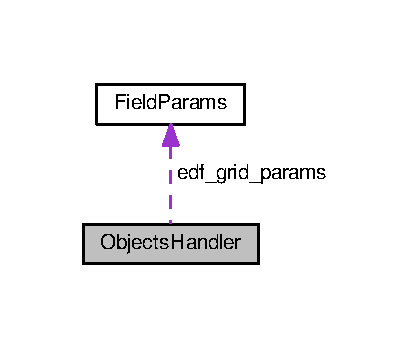
\includegraphics[width=198pt]{class_objects_handler__coll__graph}
\end{center}
\end{figure}
\subsection*{Public Member Functions}
\begin{DoxyCompactItemize}
\item 
\hyperlink{class_objects_handler_a932c6bc722daa78f4f8e31894911c4c7}{Objects\+Handler} ()
\item 
void \hyperlink{class_objects_handler_a1ac7fcad5fa6033c2435ac49f2f9dff5}{init} (ros\+::\+Node\+Handle nh)
\item 
void \hyperlink{class_objects_handler_ae6da4f0f0a265c75722e02d68d519f07}{compute\+\_\+edf} ()
\item 
\hyperlink{class_objects_handler_a5d3298d7029619c1931d3dda34278e05}{Objects\+Handler} (ros\+::\+Node\+Handle nh)
\item 
Pose\+Stamped \hyperlink{class_objects_handler_a2b9e69afe54afea0380431d8f1f5142d}{get\+\_\+target\+\_\+pose} ()
\item 
Pose\+Stamped \hyperlink{class_objects_handler_a4ac7a7bb712575c2ff6ffbf37144cf56}{get\+\_\+chaser\+\_\+pose} ()
\item 
Twist \hyperlink{class_objects_handler_aa1af309b0e964ccb6df8dede045fa32b}{get\+\_\+chaser\+\_\+velocity} ()
\item 
Twist \hyperlink{class_objects_handler_a41d48832b07a4d4276147a99dd1d31bc}{get\+\_\+chaser\+\_\+acceleration} ()
\item 
string \hyperlink{class_objects_handler_a07e9d105db04be181661dc979314de3c}{get\+\_\+world\+\_\+frame\+\_\+id} ()
\item 
octomap\+::\+Oc\+Tree $\ast$ \hyperlink{class_objects_handler_a988bdf05045c40348b34ae8beecd8884}{get\+\_\+octree\+\_\+obj\+\_\+ptr} ()
\item 
\hyperlink{struct_grid_field}{Grid\+Field} $\ast$ \hyperlink{class_objects_handler_afe849882d1feeef8316a45632381da54}{get\+\_\+edf\+\_\+grid\+\_\+ptr} ()
\item 
void \hyperlink{class_objects_handler_a5744110d979850b3e2d8896793435d0c}{octomap\+\_\+callback} (const octomap\+\_\+msgs\+::\+Octomap \&msg)
\item 
void \hyperlink{class_objects_handler_a968feba95e0707919b6c3632781510ba}{chaser\+\_\+spawn} (Pose\+Stamped spawn\+\_\+pose)
\item 
void \hyperlink{class_objects_handler_a4c56416d3583b70d181d69d900b884b5}{callback\+\_\+chaser\+\_\+init\+\_\+pose} (const geometry\+\_\+msgs\+::\+Pose\+Stamped\+Const\+Ptr \&chaser\+\_\+init\+\_\+pose)
\item 
void \hyperlink{class_objects_handler_a28ac9c7ef998a413825cddca78324f61}{callback\+\_\+chaser\+\_\+control\+\_\+pose} (const geometry\+\_\+msgs\+::\+Pose\+Stamped\+Const\+Ptr \&chaser\+\_\+control\+\_\+pose)
\begin{DoxyCompactList}\small\item\em callback function for control pose from wrapper. This is intended to replace the currnet chaser pose directly with desired pose \end{DoxyCompactList}\item 
void \hyperlink{class_objects_handler_a6896e4f9863bd1a4fbc8498d0cb20f09}{tf\+\_\+update} ()
\item 
void \hyperlink{class_objects_handler_a16cf7fca3059a03da4ec795f2af7fb74}{publish} ()
\item 
vector$<$ Point $>$ \hyperlink{class_objects_handler_a4793f1ed257c849b28f0386f635ee714}{get\+\_\+prediction\+\_\+seq} ()
\end{DoxyCompactItemize}
\subsection*{Public Attributes}
\begin{DoxyCompactItemize}
\item 
bool \hyperlink{class_objects_handler_a56f70ac04c01e8b948a4b44fa5670f49}{is\+\_\+octomap\+\_\+full} = false
\item 
bool \hyperlink{class_objects_handler_a86f8528ff5697c87fc6a3fcd6ba0f42c}{is\+\_\+chaser\+\_\+recieved} = false
\item 
bool \hyperlink{class_objects_handler_acf1ef1b318defc2a39d87cea72689478}{is\+\_\+map\+\_\+recieved} = false
\item 
bool \hyperlink{class_objects_handler_a7691f3e1ec58e55ead30c50c555f169a}{is\+\_\+target\+\_\+recieved} = false
\item 
bool \hyperlink{class_objects_handler_a88fb913340c535df81f3b7ae5f06df61}{is\+\_\+control\+\_\+received} = false
\item 
bool \hyperlink{class_objects_handler_a16165ae7c0167ba8d2a0151a8a4fbfd5}{is\+\_\+chaser\+\_\+spawned} = false
\item 
bool \hyperlink{class_objects_handler_acaefe98eb412d4c32cda2bf0bd602ae7}{is\+\_\+insert\+\_\+permit} = false
\item 
bool \hyperlink{class_objects_handler_ad8d1ea6646024f0a03e154a7c2c07682}{is\+\_\+path\+\_\+solved} = false
\end{DoxyCompactItemize}
\subsection*{Private Attributes}
\begin{DoxyCompactItemize}
\item 
ros\+::\+Subscriber \hyperlink{class_objects_handler_a3b384ae3f8f66557b1c1ac04523fb330}{sub\+\_\+octomap}
\item 
ros\+::\+Subscriber \hyperlink{class_objects_handler_a9a2e098b85260b71c88b81dadd6ca58a}{sub\+\_\+chaser\+\_\+init\+\_\+pose}
\item 
ros\+::\+Subscriber \hyperlink{class_objects_handler_adc3a2895e97bb2349fb5cb71d4eec191}{sub\+\_\+chaser\+\_\+control\+\_\+pose}
\item 
ros\+::\+Publisher \hyperlink{class_objects_handler_a86a1f98983b533f77bf17867affb5251}{pub\+\_\+edf}
\item 
visualization\+\_\+msgs\+::\+Marker \hyperlink{class_objects_handler_ad6904dcaaad790234569760df0fb0ac2}{markers\+\_\+edf}
\item 
tf\+::\+Transform\+Listener $\ast$ \hyperlink{class_objects_handler_aea45bba31aa769008386100725bda66b}{tf\+\_\+listener}
\item 
tf\+::\+Transform\+Broadcaster $\ast$ \hyperlink{class_objects_handler_af49de4eabb124e2ee6c9e12ebb31bca3}{tf\+\_\+talker}
\item 
string \hyperlink{class_objects_handler_a1c0586ae7467bb8a3df8ad247ac7b10b}{world\+\_\+frame\+\_\+id}
\item 
string \hyperlink{class_objects_handler_a3e8d08bf5d76d69f1768b53fd799953c}{chaser\+\_\+frame\+\_\+id}
\item 
string \hyperlink{class_objects_handler_a7a616768386c4c7da9af4da3d07bd936}{target\+\_\+frame\+\_\+id}
\item 
string \hyperlink{class_objects_handler_a70b5e252a180d919653c7b53aff6f534}{octomap\+\_\+topic\+\_\+name}
\item 
Pose\+Stamped \hyperlink{class_objects_handler_ad436bfd8b262f473f0e4ca92b3c3402b}{target\+\_\+pose}
\item 
Pose\+Stamped \hyperlink{class_objects_handler_a79fd5f872a40cca5ea599f1e83dcb3ad}{chaser\+\_\+pose}
\item 
Twist \hyperlink{class_objects_handler_a74e3f3b4bf263711c389190a595368e2}{chaser\+\_\+vel}
\item 
Twist \hyperlink{class_objects_handler_a36db60068ada56b9142b3d6ef0437749}{chaser\+\_\+acc}
\item 
shared\+\_\+ptr$<$ octomap\+::\+Oc\+Tree $>$ \hyperlink{class_objects_handler_a76ad7ca7513755408c02dd36dea94c6e}{octree\+\_\+ptr}
\item 
Dynamic\+E\+D\+T\+Octomap $\ast$ \hyperlink{class_objects_handler_aa96d8c71f5e8c6423c88d3302220d4cf}{edf\+\_\+ptr}
\item 
shared\+\_\+ptr$<$ \hyperlink{struct_grid_field}{Grid\+Field} $>$ \hyperlink{class_objects_handler_af2063609510d5ad8f136a275b0d127c1}{edf\+\_\+grid\+\_\+ptr}
\item 
double \hyperlink{class_objects_handler_ac8c10c7a10aeb8abf1a44b7361f646e6}{min\+\_\+z}
\item 
double \hyperlink{class_objects_handler_aa991434e17ca1144c80633ff7530534c}{chaser\+\_\+init\+\_\+z}
\item 
double \hyperlink{class_objects_handler_a577e8b62f1e55d36330048fb9fd3a432}{edf\+\_\+max\+\_\+viz\+\_\+dist}
\item 
double \hyperlink{class_objects_handler_ae71885df3c4e28f45be7bb0e5a383293}{edf\+\_\+max\+\_\+dist}
\item 
\hyperlink{struct_field_params}{Field\+Params} \hyperlink{class_objects_handler_a46ed8cfd250b183909a7d3a1f56cee6b}{edf\+\_\+grid\+\_\+params}
\item 
int \hyperlink{class_objects_handler_a95908d5b00f62b629dc7f20acb714292}{run\+\_\+mode}
\end{DoxyCompactItemize}


\subsection{Detailed Description}


\subsection{Constructor \& Destructor Documentation}
\index{Objects\+Handler@{Objects\+Handler}!Objects\+Handler@{Objects\+Handler}}
\index{Objects\+Handler@{Objects\+Handler}!Objects\+Handler@{Objects\+Handler}}
\subsubsection[{\texorpdfstring{Objects\+Handler()}{ObjectsHandler()}}]{\setlength{\rightskip}{0pt plus 5cm}Objects\+Handler\+::\+Objects\+Handler (
\begin{DoxyParamCaption}
{}
\end{DoxyParamCaption}
)\hspace{0.3cm}{\ttfamily [inline]}}\hypertarget{class_objects_handler_a932c6bc722daa78f4f8e31894911c4c7}{}\label{class_objects_handler_a932c6bc722daa78f4f8e31894911c4c7}

\begin{DoxyCode}
56 \{\};
\end{DoxyCode}
\index{Objects\+Handler@{Objects\+Handler}!Objects\+Handler@{Objects\+Handler}}
\index{Objects\+Handler@{Objects\+Handler}!Objects\+Handler@{Objects\+Handler}}
\subsubsection[{\texorpdfstring{Objects\+Handler(ros\+::\+Node\+Handle nh)}{ObjectsHandler(ros::NodeHandle nh)}}]{\setlength{\rightskip}{0pt plus 5cm}Objects\+Handler\+::\+Objects\+Handler (
\begin{DoxyParamCaption}
\item[{ros\+::\+Node\+Handle}]{nh}
\end{DoxyParamCaption}
)}\hypertarget{class_objects_handler_a5d3298d7029619c1931d3dda34278e05}{}\label{class_objects_handler_a5d3298d7029619c1931d3dda34278e05}

\begin{DoxyCode}
3 \{\};
\end{DoxyCode}


\subsection{Member Function Documentation}
\index{Objects\+Handler@{Objects\+Handler}!callback\+\_\+chaser\+\_\+control\+\_\+pose@{callback\+\_\+chaser\+\_\+control\+\_\+pose}}
\index{callback\+\_\+chaser\+\_\+control\+\_\+pose@{callback\+\_\+chaser\+\_\+control\+\_\+pose}!Objects\+Handler@{Objects\+Handler}}
\subsubsection[{\texorpdfstring{callback\+\_\+chaser\+\_\+control\+\_\+pose(const geometry\+\_\+msgs\+::\+Pose\+Stamped\+Const\+Ptr \&chaser\+\_\+control\+\_\+pose)}{callback_chaser_control_pose(const geometry_msgs::PoseStampedConstPtr &chaser_control_pose)}}]{\setlength{\rightskip}{0pt plus 5cm}void Objects\+Handler\+::callback\+\_\+chaser\+\_\+control\+\_\+pose (
\begin{DoxyParamCaption}
\item[{const geometry\+\_\+msgs\+::\+Pose\+Stamped\+Const\+Ptr \&}]{chaser\+\_\+control\+\_\+pose}
\end{DoxyParamCaption}
)}\hypertarget{class_objects_handler_a28ac9c7ef998a413825cddca78324f61}{}\label{class_objects_handler_a28ac9c7ef998a413825cddca78324f61}


callback function for control pose from wrapper. This is intended to replace the currnet chaser pose directly with desired pose 


\begin{DoxyParams}{Parameters}
{\em chaser\+\_\+control\+\_\+pose} & \\
\hline
\end{DoxyParams}

\begin{DoxyCode}
278                                                                                                            
       \{
279     \textcolor{keywordflow}{if}(\hyperlink{class_objects_handler_a95908d5b00f62b629dc7f20acb714292}{run\_mode} == 0 and \hyperlink{class_objects_handler_ad8d1ea6646024f0a03e154a7c2c07682}{is\_path\_solved})\{
280         \hyperlink{class_objects_handler_a79fd5f872a40cca5ea599f1e83dcb3ad}{chaser\_pose} = *chaser\_control\_pose;
281     \}
282     
283 \}
\end{DoxyCode}
\index{Objects\+Handler@{Objects\+Handler}!callback\+\_\+chaser\+\_\+init\+\_\+pose@{callback\+\_\+chaser\+\_\+init\+\_\+pose}}
\index{callback\+\_\+chaser\+\_\+init\+\_\+pose@{callback\+\_\+chaser\+\_\+init\+\_\+pose}!Objects\+Handler@{Objects\+Handler}}
\subsubsection[{\texorpdfstring{callback\+\_\+chaser\+\_\+init\+\_\+pose(const geometry\+\_\+msgs\+::\+Pose\+Stamped\+Const\+Ptr \&chaser\+\_\+init\+\_\+pose)}{callback_chaser_init_pose(const geometry_msgs::PoseStampedConstPtr &chaser_init_pose)}}]{\setlength{\rightskip}{0pt plus 5cm}void Objects\+Handler\+::callback\+\_\+chaser\+\_\+init\+\_\+pose (
\begin{DoxyParamCaption}
\item[{const geometry\+\_\+msgs\+::\+Pose\+Stamped\+Const\+Ptr \&}]{chaser\+\_\+init\+\_\+pose}
\end{DoxyParamCaption}
)}\hypertarget{class_objects_handler_a4c56416d3583b70d181d69d900b884b5}{}\label{class_objects_handler_a4c56416d3583b70d181d69d900b884b5}

\begin{DoxyCode}
269                                                                                                       \{
270 
271     \hyperlink{class_objects_handler_a968feba95e0707919b6c3632781510ba}{chaser\_spawn}(*chaser\_init\_pose);    
272 \}
\end{DoxyCode}
\index{Objects\+Handler@{Objects\+Handler}!chaser\+\_\+spawn@{chaser\+\_\+spawn}}
\index{chaser\+\_\+spawn@{chaser\+\_\+spawn}!Objects\+Handler@{Objects\+Handler}}
\subsubsection[{\texorpdfstring{chaser\+\_\+spawn(\+Pose\+Stamped spawn\+\_\+pose)}{chaser_spawn(PoseStamped spawn_pose)}}]{\setlength{\rightskip}{0pt plus 5cm}void Objects\+Handler\+::chaser\+\_\+spawn (
\begin{DoxyParamCaption}
\item[{Pose\+Stamped}]{spawn\+\_\+pose}
\end{DoxyParamCaption}
)}\hypertarget{class_objects_handler_a968feba95e0707919b6c3632781510ba}{}\label{class_objects_handler_a968feba95e0707919b6c3632781510ba}

\begin{DoxyCode}
253                                                        \{
254     ROS\_INFO\_ONCE(\textcolor{stringliteral}{"[Objects handler] spawning chaser."}); 
255     
256     \hyperlink{class_objects_handler_a86f8528ff5697c87fc6a3fcd6ba0f42c}{is\_chaser\_recieved} = \textcolor{keyword}{true};
257     \hyperlink{class_objects_handler_a16165ae7c0167ba8d2a0151a8a4fbfd5}{is\_chaser\_spawned} = \textcolor{keyword}{true};    
258     
259     \textcolor{keywordflow}{if}(\hyperlink{class_objects_handler_a95908d5b00f62b629dc7f20acb714292}{run\_mode} == 0)\{ \textcolor{comment}{// without gazebo : update chaser pose}
260         \hyperlink{class_objects_handler_a79fd5f872a40cca5ea599f1e83dcb3ad}{chaser\_pose} = spawn\_pose;
261         \hyperlink{class_objects_handler_a79fd5f872a40cca5ea599f1e83dcb3ad}{chaser\_pose}.pose.position.z = \hyperlink{class_objects_handler_aa991434e17ca1144c80633ff7530534c}{chaser\_init\_z};
262 
263     \}\textcolor{keywordflow}{else}\{ \textcolor{comment}{// with gazebo : nothing happen }
264         ROS\_WARN(\textcolor{stringliteral}{"[Object Handler] gazebo mode. No virtual spawning happens"});        
265     \}
266 
267 \}
\end{DoxyCode}
\index{Objects\+Handler@{Objects\+Handler}!compute\+\_\+edf@{compute\+\_\+edf}}
\index{compute\+\_\+edf@{compute\+\_\+edf}!Objects\+Handler@{Objects\+Handler}}
\subsubsection[{\texorpdfstring{compute\+\_\+edf()}{compute_edf()}}]{\setlength{\rightskip}{0pt plus 5cm}void Objects\+Handler\+::compute\+\_\+edf (
\begin{DoxyParamCaption}
{}
\end{DoxyParamCaption}
)}\hypertarget{class_objects_handler_ae6da4f0f0a265c75722e02d68d519f07}{}\label{class_objects_handler_ae6da4f0f0a265c75722e02d68d519f07}

\begin{DoxyCode}
222                                 \{
223 
224     \textcolor{keywordflow}{for}(\textcolor{keywordtype}{int} ix = 0 ; ix<\hyperlink{class_objects_handler_af2063609510d5ad8f136a275b0d127c1}{edf\_grid\_ptr}.get()->Nx ; ix++)
225         \textcolor{keywordflow}{for}(\textcolor{keywordtype}{int} iy = 0 ; iy<\hyperlink{class_objects_handler_af2063609510d5ad8f136a275b0d127c1}{edf\_grid\_ptr}.get()->Ny ; iy++)
226             \textcolor{keywordflow}{for}(\textcolor{keywordtype}{int} iz = 0 ; iz<\hyperlink{class_objects_handler_af2063609510d5ad8f136a275b0d127c1}{edf\_grid\_ptr}.get()->Nz ; iz++)\{
227                 Point eval\_pnt = \hyperlink{class_objects_handler_af2063609510d5ad8f136a275b0d127c1}{edf\_grid\_ptr}.get()->getCellPnt(Vector3i(ix,iy,iz));  
228                 \textcolor{comment}{// query edf value from edf mapper                       }
229                 \textcolor{keywordtype}{float} dist\_val = \hyperlink{class_objects_handler_aa96d8c71f5e8c6423c88d3302220d4cf}{edf\_ptr}->getDistance(octomap::point3d(eval\_pnt.x,eval\_pnt.y,
      eval\_pnt.z));
230 
231                 \textcolor{comment}{// edf value assign to homogenous grid  }
232                 \hyperlink{class_objects_handler_af2063609510d5ad8f136a275b0d127c1}{edf\_grid\_ptr}.get()->field\_vals[ix][iy][iz] = dist\_val;
233 
234                 \textcolor{comment}{// marker generation}
235                 \textcolor{keywordflow}{if}(dist\_val<\hyperlink{class_objects_handler_a577e8b62f1e55d36330048fb9fd3a432}{edf\_max\_viz\_dist})\{                
236                     \textcolor{comment}{// color }
237                     std\_msgs::ColorRGBA color;                    
238                     \hyperlink{_common_8h_a4b2e4b6698ff92678b23392dc111b36d}{get\_color\_dist}(dist\_val,color,\hyperlink{class_objects_handler_a577e8b62f1e55d36330048fb9fd3a432}{edf\_max\_viz\_dist});
239 
240                     \textcolor{comment}{// marker }
241                     \hyperlink{class_objects_handler_ad6904dcaaad790234569760df0fb0ac2}{markers\_edf}.points.push\_back(eval\_pnt);
242                     \hyperlink{class_objects_handler_ad6904dcaaad790234569760df0fb0ac2}{markers\_edf}.colors.push\_back(color);                    
243                 \}
244             \}    
245 
246 \}
\end{DoxyCode}
\index{Objects\+Handler@{Objects\+Handler}!get\+\_\+chaser\+\_\+acceleration@{get\+\_\+chaser\+\_\+acceleration}}
\index{get\+\_\+chaser\+\_\+acceleration@{get\+\_\+chaser\+\_\+acceleration}!Objects\+Handler@{Objects\+Handler}}
\subsubsection[{\texorpdfstring{get\+\_\+chaser\+\_\+acceleration()}{get_chaser_acceleration()}}]{\setlength{\rightskip}{0pt plus 5cm}Twist Objects\+Handler\+::get\+\_\+chaser\+\_\+acceleration (
\begin{DoxyParamCaption}
{}
\end{DoxyParamCaption}
)}\hypertarget{class_objects_handler_a41d48832b07a4d4276147a99dd1d31bc}{}\label{class_objects_handler_a41d48832b07a4d4276147a99dd1d31bc}

\begin{DoxyCode}
120 \{\textcolor{keywordflow}{return} \hyperlink{class_objects_handler_a36db60068ada56b9142b3d6ef0437749}{chaser\_acc};\};
\end{DoxyCode}
\index{Objects\+Handler@{Objects\+Handler}!get\+\_\+chaser\+\_\+pose@{get\+\_\+chaser\+\_\+pose}}
\index{get\+\_\+chaser\+\_\+pose@{get\+\_\+chaser\+\_\+pose}!Objects\+Handler@{Objects\+Handler}}
\subsubsection[{\texorpdfstring{get\+\_\+chaser\+\_\+pose()}{get_chaser_pose()}}]{\setlength{\rightskip}{0pt plus 5cm}Pose\+Stamped Objects\+Handler\+::get\+\_\+chaser\+\_\+pose (
\begin{DoxyParamCaption}
{}
\end{DoxyParamCaption}
)}\hypertarget{class_objects_handler_a4ac7a7bb712575c2ff6ffbf37144cf56}{}\label{class_objects_handler_a4ac7a7bb712575c2ff6ffbf37144cf56}

\begin{DoxyCode}
118 \{\textcolor{keywordflow}{return} \hyperlink{class_objects_handler_a79fd5f872a40cca5ea599f1e83dcb3ad}{chaser\_pose};\};
\end{DoxyCode}
\index{Objects\+Handler@{Objects\+Handler}!get\+\_\+chaser\+\_\+velocity@{get\+\_\+chaser\+\_\+velocity}}
\index{get\+\_\+chaser\+\_\+velocity@{get\+\_\+chaser\+\_\+velocity}!Objects\+Handler@{Objects\+Handler}}
\subsubsection[{\texorpdfstring{get\+\_\+chaser\+\_\+velocity()}{get_chaser_velocity()}}]{\setlength{\rightskip}{0pt plus 5cm}Twist Objects\+Handler\+::get\+\_\+chaser\+\_\+velocity (
\begin{DoxyParamCaption}
{}
\end{DoxyParamCaption}
)}\hypertarget{class_objects_handler_aa1af309b0e964ccb6df8dede045fa32b}{}\label{class_objects_handler_aa1af309b0e964ccb6df8dede045fa32b}

\begin{DoxyCode}
119 \{\textcolor{keywordflow}{return} \hyperlink{class_objects_handler_a74e3f3b4bf263711c389190a595368e2}{chaser\_vel};\};
\end{DoxyCode}
\index{Objects\+Handler@{Objects\+Handler}!get\+\_\+edf\+\_\+grid\+\_\+ptr@{get\+\_\+edf\+\_\+grid\+\_\+ptr}}
\index{get\+\_\+edf\+\_\+grid\+\_\+ptr@{get\+\_\+edf\+\_\+grid\+\_\+ptr}!Objects\+Handler@{Objects\+Handler}}
\subsubsection[{\texorpdfstring{get\+\_\+edf\+\_\+grid\+\_\+ptr()}{get_edf_grid_ptr()}}]{\setlength{\rightskip}{0pt plus 5cm}{\bf Grid\+Field} $\ast$ Objects\+Handler\+::get\+\_\+edf\+\_\+grid\+\_\+ptr (
\begin{DoxyParamCaption}
{}
\end{DoxyParamCaption}
)}\hypertarget{class_objects_handler_afe849882d1feeef8316a45632381da54}{}\label{class_objects_handler_afe849882d1feeef8316a45632381da54}

\begin{DoxyCode}
123 \{\textcolor{keywordflow}{return} \hyperlink{class_objects_handler_af2063609510d5ad8f136a275b0d127c1}{edf\_grid\_ptr}.get();\};
\end{DoxyCode}
\index{Objects\+Handler@{Objects\+Handler}!get\+\_\+octree\+\_\+obj\+\_\+ptr@{get\+\_\+octree\+\_\+obj\+\_\+ptr}}
\index{get\+\_\+octree\+\_\+obj\+\_\+ptr@{get\+\_\+octree\+\_\+obj\+\_\+ptr}!Objects\+Handler@{Objects\+Handler}}
\subsubsection[{\texorpdfstring{get\+\_\+octree\+\_\+obj\+\_\+ptr()}{get_octree_obj_ptr()}}]{\setlength{\rightskip}{0pt plus 5cm}octomap\+::\+Oc\+Tree $\ast$ Objects\+Handler\+::get\+\_\+octree\+\_\+obj\+\_\+ptr (
\begin{DoxyParamCaption}
{}
\end{DoxyParamCaption}
)}\hypertarget{class_objects_handler_a988bdf05045c40348b34ae8beecd8884}{}\label{class_objects_handler_a988bdf05045c40348b34ae8beecd8884}

\begin{DoxyCode}
122 \{\textcolor{keywordflow}{return} \hyperlink{class_objects_handler_a76ad7ca7513755408c02dd36dea94c6e}{octree\_ptr}.get();\};
\end{DoxyCode}
\index{Objects\+Handler@{Objects\+Handler}!get\+\_\+prediction\+\_\+seq@{get\+\_\+prediction\+\_\+seq}}
\index{get\+\_\+prediction\+\_\+seq@{get\+\_\+prediction\+\_\+seq}!Objects\+Handler@{Objects\+Handler}}
\subsubsection[{\texorpdfstring{get\+\_\+prediction\+\_\+seq()}{get_prediction_seq()}}]{\setlength{\rightskip}{0pt plus 5cm}vector$<$ Point $>$ Objects\+Handler\+::get\+\_\+prediction\+\_\+seq (
\begin{DoxyParamCaption}
{}
\end{DoxyParamCaption}
)}\hypertarget{class_objects_handler_a4793f1ed257c849b28f0386f635ee714}{}\label{class_objects_handler_a4793f1ed257c849b28f0386f635ee714}

\begin{DoxyCode}
286                                                 \{
287     
288     
289 \}
\end{DoxyCode}
\index{Objects\+Handler@{Objects\+Handler}!get\+\_\+target\+\_\+pose@{get\+\_\+target\+\_\+pose}}
\index{get\+\_\+target\+\_\+pose@{get\+\_\+target\+\_\+pose}!Objects\+Handler@{Objects\+Handler}}
\subsubsection[{\texorpdfstring{get\+\_\+target\+\_\+pose()}{get_target_pose()}}]{\setlength{\rightskip}{0pt plus 5cm}Pose\+Stamped Objects\+Handler\+::get\+\_\+target\+\_\+pose (
\begin{DoxyParamCaption}
{}
\end{DoxyParamCaption}
)}\hypertarget{class_objects_handler_a2b9e69afe54afea0380431d8f1f5142d}{}\label{class_objects_handler_a2b9e69afe54afea0380431d8f1f5142d}

\begin{DoxyCode}
111                                             \{
112     PoseStamped pose(\hyperlink{class_objects_handler_ad436bfd8b262f473f0e4ca92b3c3402b}{target\_pose}); 
113     pose.pose.position.z = \hyperlink{class_objects_handler_ac8c10c7a10aeb8abf1a44b7361f646e6}{min\_z}; 
114     \textcolor{keywordflow}{return} pose;
115 \};
\end{DoxyCode}
\index{Objects\+Handler@{Objects\+Handler}!get\+\_\+world\+\_\+frame\+\_\+id@{get\+\_\+world\+\_\+frame\+\_\+id}}
\index{get\+\_\+world\+\_\+frame\+\_\+id@{get\+\_\+world\+\_\+frame\+\_\+id}!Objects\+Handler@{Objects\+Handler}}
\subsubsection[{\texorpdfstring{get\+\_\+world\+\_\+frame\+\_\+id()}{get_world_frame_id()}}]{\setlength{\rightskip}{0pt plus 5cm}string Objects\+Handler\+::get\+\_\+world\+\_\+frame\+\_\+id (
\begin{DoxyParamCaption}
{}
\end{DoxyParamCaption}
)}\hypertarget{class_objects_handler_a07e9d105db04be181661dc979314de3c}{}\label{class_objects_handler_a07e9d105db04be181661dc979314de3c}

\begin{DoxyCode}
121 \{\textcolor{keywordflow}{return} \hyperlink{class_objects_handler_a1c0586ae7467bb8a3df8ad247ac7b10b}{world\_frame\_id};\};
\end{DoxyCode}
\index{Objects\+Handler@{Objects\+Handler}!init@{init}}
\index{init@{init}!Objects\+Handler@{Objects\+Handler}}
\subsubsection[{\texorpdfstring{init(ros\+::\+Node\+Handle nh)}{init(ros::NodeHandle nh)}}]{\setlength{\rightskip}{0pt plus 5cm}void Objects\+Handler\+::init (
\begin{DoxyParamCaption}
\item[{ros\+::\+Node\+Handle}]{nh}
\end{DoxyParamCaption}
)}\hypertarget{class_objects_handler_a1ac7fcad5fa6033c2435ac49f2f9dff5}{}\label{class_objects_handler_a1ac7fcad5fa6033c2435ac49f2f9dff5}

\begin{DoxyCode}
5                                          \{
6 
7     \textcolor{comment}{// parameters}
8     nh.param<\textcolor{keywordtype}{string}>(\textcolor{stringliteral}{"world\_frame\_id"},this->\hyperlink{class_objects_handler_a1c0586ae7467bb8a3df8ad247ac7b10b}{world\_frame\_id},\textcolor{stringliteral}{"/world"});
9     nh.param<\textcolor{keywordtype}{string}>(\textcolor{stringliteral}{"target\_frame\_id"},this->\hyperlink{class_objects_handler_a7a616768386c4c7da9af4da3d07bd936}{target\_frame\_id},\textcolor{stringliteral}{"/target\_\_base\_footprint"});
10     nh.param<\textcolor{keywordtype}{string}>(\textcolor{stringliteral}{"chaser\_frame\_id"},this->\hyperlink{class_objects_handler_a3e8d08bf5d76d69f1768b53fd799953c}{chaser\_frame\_id},\textcolor{stringliteral}{"/firefly/base\_link"}); 
11 
12     \textcolor{comment}{// for chaser spawning }
13      
14     \textcolor{comment}{// edf grid param}
15     nh.param(\textcolor{stringliteral}{"min\_z"},\hyperlink{class_objects_handler_ac8c10c7a10aeb8abf1a44b7361f646e6}{min\_z},0.4);   
16     nh.param(\textcolor{stringliteral}{"chaser\_init\_z"},\hyperlink{class_objects_handler_aa991434e17ca1144c80633ff7530534c}{chaser\_init\_z},1.0);             
17     nh.param(\textcolor{stringliteral}{"edf\_max\_dist"},\hyperlink{class_objects_handler_ae71885df3c4e28f45be7bb0e5a383293}{edf\_max\_dist},2.0);  
18     nh.param(\textcolor{stringliteral}{"edf\_max\_plot\_dist"},\hyperlink{class_objects_handler_a577e8b62f1e55d36330048fb9fd3a432}{edf\_max\_viz\_dist},0.5);  
19     nh.param(\textcolor{stringliteral}{"edf\_resolution"},\hyperlink{class_objects_handler_a46ed8cfd250b183909a7d3a1f56cee6b}{edf\_grid\_params}.\hyperlink{struct_field_params_a520406c76b3abf392401626bc2161370}{resolution},0.5);  
20     nh.param(\textcolor{stringliteral}{"edf\_stride\_resolution"},\hyperlink{class_objects_handler_a46ed8cfd250b183909a7d3a1f56cee6b}{edf\_grid\_params}.
      \hyperlink{struct_field_params_ae6eabaa6e593c9dbac48b2f96bea80ec}{ray\_stride\_res},0.3);  
21     nh.param(\textcolor{stringliteral}{"run\_mode"},\hyperlink{class_objects_handler_a95908d5b00f62b629dc7f20acb714292}{run\_mode},0);  
22 
23 
24     \hyperlink{class_objects_handler_ad436bfd8b262f473f0e4ca92b3c3402b}{target\_pose}.header.frame\_id = \hyperlink{class_objects_handler_a1c0586ae7467bb8a3df8ad247ac7b10b}{world\_frame\_id};
25     \hyperlink{class_objects_handler_a79fd5f872a40cca5ea599f1e83dcb3ad}{chaser\_pose}.header.frame\_id = \hyperlink{class_objects_handler_a1c0586ae7467bb8a3df8ad247ac7b10b}{world\_frame\_id};
26     \hyperlink{class_objects_handler_ad6904dcaaad790234569760df0fb0ac2}{markers\_edf}.header.frame\_id = \hyperlink{class_objects_handler_a1c0586ae7467bb8a3df8ad247ac7b10b}{world\_frame\_id};
27 
28     \hyperlink{class_objects_handler_ad6904dcaaad790234569760df0fb0ac2}{markers\_edf}.action = visualization\_msgs::Marker::ADD;
29     \hyperlink{class_objects_handler_ad6904dcaaad790234569760df0fb0ac2}{markers\_edf}.type = visualization\_msgs::Marker::CUBE\_LIST;      
30     \hyperlink{class_objects_handler_ad6904dcaaad790234569760df0fb0ac2}{markers\_edf}.pose.orientation.x = 0;
31     \hyperlink{class_objects_handler_ad6904dcaaad790234569760df0fb0ac2}{markers\_edf}.pose.orientation.y = 0;
32     \hyperlink{class_objects_handler_ad6904dcaaad790234569760df0fb0ac2}{markers\_edf}.pose.orientation.z = 0;
33     \hyperlink{class_objects_handler_ad6904dcaaad790234569760df0fb0ac2}{markers\_edf}.pose.orientation.w = 1;                  
34     \hyperlink{class_objects_handler_ad6904dcaaad790234569760df0fb0ac2}{markers\_edf}.scale.x = \hyperlink{class_objects_handler_a46ed8cfd250b183909a7d3a1f56cee6b}{edf\_grid\_params}.\hyperlink{struct_field_params_a520406c76b3abf392401626bc2161370}{resolution};
35     \hyperlink{class_objects_handler_ad6904dcaaad790234569760df0fb0ac2}{markers\_edf}.scale.y = \hyperlink{class_objects_handler_a46ed8cfd250b183909a7d3a1f56cee6b}{edf\_grid\_params}.\hyperlink{struct_field_params_a520406c76b3abf392401626bc2161370}{resolution};
36     \hyperlink{class_objects_handler_ad6904dcaaad790234569760df0fb0ac2}{markers\_edf}.scale.z = \hyperlink{class_objects_handler_a46ed8cfd250b183909a7d3a1f56cee6b}{edf\_grid\_params}.\hyperlink{struct_field_params_a520406c76b3abf392401626bc2161370}{resolution};
37     
38     
39     \textcolor{comment}{// topics }
40     \hyperlink{class_objects_handler_aea45bba31aa769008386100725bda66b}{tf\_listener} = \textcolor{keyword}{new} (tf::TransformListener);
41     \hyperlink{class_objects_handler_af49de4eabb124e2ee6c9e12ebb31bca3}{tf\_talker} = \textcolor{keyword}{new} (tf::TransformBroadcaster);
42 
43     \hyperlink{class_objects_handler_a86a1f98983b533f77bf17867affb5251}{pub\_edf} = nh.advertise<visualization\_msgs::Marker>(\textcolor{stringliteral}{"edf\_grid"},1);
44 
45     \textcolor{comment}{// octomap            }
46     nh.param(\textcolor{stringliteral}{"is\_octomap\_full"},this->\hyperlink{class_objects_handler_a56f70ac04c01e8b948a4b44fa5670f49}{is\_octomap\_full},\textcolor{keyword}{true});
47     \hyperlink{class_objects_handler_a76ad7ca7513755408c02dd36dea94c6e}{octree\_ptr}.reset(\textcolor{keyword}{new} octomap::OcTree(0.1)); \textcolor{comment}{// arbitrary init}
48     \textcolor{keywordflow}{if} (\hyperlink{class_objects_handler_a56f70ac04c01e8b948a4b44fa5670f49}{is\_octomap\_full})
49         \hyperlink{class_objects_handler_a3b384ae3f8f66557b1c1ac04523fb330}{sub\_octomap} = nh.subscribe(\textcolor{stringliteral}{"/octomap\_full"},1,&
      \hyperlink{class_objects_handler_a5744110d979850b3e2d8896793435d0c}{ObjectsHandler::octomap\_callback},\textcolor{keyword}{this});   
50     \textcolor{keywordflow}{else}
51         \hyperlink{class_objects_handler_a3b384ae3f8f66557b1c1ac04523fb330}{sub\_octomap} = nh.subscribe(\textcolor{stringliteral}{"/octomap\_binary"},1,&
      \hyperlink{class_objects_handler_a5744110d979850b3e2d8896793435d0c}{ObjectsHandler::octomap\_callback},\textcolor{keyword}{this});   
52 
53     \hyperlink{class_objects_handler_a9a2e098b85260b71c88b81dadd6ca58a}{sub\_chaser\_init\_pose} = nh.subscribe(\textcolor{stringliteral}{"/chaser\_init\_pose"},1,&
      \hyperlink{class_objects_handler_a4c56416d3583b70d181d69d900b884b5}{ObjectsHandler::callback\_chaser\_init\_pose},\textcolor{keyword}{this});
54     \hyperlink{class_objects_handler_adc3a2895e97bb2349fb5cb71d4eec191}{sub\_chaser\_control\_pose} = nh.subscribe(\textcolor{stringliteral}{"mav\_pose\_desired"},1,&
      \hyperlink{class_objects_handler_a28ac9c7ef998a413825cddca78324f61}{ObjectsHandler::callback\_chaser\_control\_pose},\textcolor{keyword}{this});
55     
56     ROS\_INFO(\textcolor{stringliteral}{"Object handler initialized."}); 
57 \}
\end{DoxyCode}
\index{Objects\+Handler@{Objects\+Handler}!octomap\+\_\+callback@{octomap\+\_\+callback}}
\index{octomap\+\_\+callback@{octomap\+\_\+callback}!Objects\+Handler@{Objects\+Handler}}
\subsubsection[{\texorpdfstring{octomap\+\_\+callback(const octomap\+\_\+msgs\+::\+Octomap \&msg)}{octomap_callback(const octomap_msgs::Octomap &msg)}}]{\setlength{\rightskip}{0pt plus 5cm}void Objects\+Handler\+::octomap\+\_\+callback (
\begin{DoxyParamCaption}
\item[{const octomap\+\_\+msgs\+::\+Octomap \&}]{msg}
\end{DoxyParamCaption}
)}\hypertarget{class_objects_handler_a5744110d979850b3e2d8896793435d0c}{}\label{class_objects_handler_a5744110d979850b3e2d8896793435d0c}

\begin{DoxyCode}
59                                                                    \{
60     \textcolor{comment}{// we receive only once from octoamp server}
61     \textcolor{keywordflow}{if} (not \hyperlink{class_objects_handler_acf1ef1b318defc2a39d87cea72689478}{is\_map\_recieved})\{
62 
63         \textcolor{comment}{// octomap subscribing }
64         octomap::AbstractOcTree* octree;
65 
66         \textcolor{keywordflow}{if}(\hyperlink{class_objects_handler_a56f70ac04c01e8b948a4b44fa5670f49}{is\_octomap\_full})
67             octree=octomap\_msgs::fullMsgToMap(msg);
68         \textcolor{keywordflow}{else}
69             octree=octomap\_msgs::binaryMsgToMap(msg);
70 
71         this->\hyperlink{class_objects_handler_a76ad7ca7513755408c02dd36dea94c6e}{octree\_ptr}.reset((dynamic\_cast<octomap::OcTree*>(octree)));
72 
73         ROS\_INFO\_ONCE(\textcolor{stringliteral}{"[Objects handler] octomap received."});
74         \textcolor{keywordtype}{double} x,y,z;
75         \hyperlink{class_objects_handler_a76ad7ca7513755408c02dd36dea94c6e}{octree\_ptr}.get()->getMetricMin(x,y,z);
76         octomap::point3d boundary\_min(x,y,z); 
77         boundary\_min.z() = \hyperlink{class_objects_handler_ac8c10c7a10aeb8abf1a44b7361f646e6}{min\_z};
78         \hyperlink{class_objects_handler_a76ad7ca7513755408c02dd36dea94c6e}{octree\_ptr}.get()->getMetricMax(x,y,z);
79         octomap::point3d boundary\_max(x,y,z); 
80 
81         \textcolor{keywordtype}{bool} unknownAsOccupied = \textcolor{keyword}{false};
82 
83 
84         std::chrono::steady\_clock::time\_point begin = std::chrono::steady\_clock::now();
85 
86         \textcolor{comment}{// Euclidean distance transform  }
87         \hyperlink{class_objects_handler_aa96d8c71f5e8c6423c88d3302220d4cf}{edf\_ptr} = \textcolor{keyword}{new} DynamicEDTOctomap(\hyperlink{class_objects_handler_ae71885df3c4e28f45be7bb0e5a383293}{edf\_max\_dist},
      \hyperlink{class_objects_handler_a76ad7ca7513755408c02dd36dea94c6e}{octree\_ptr}.get(),
88         boundary\_min,
89         boundary\_max,unknownAsOccupied);
90         \hyperlink{class_objects_handler_aa96d8c71f5e8c6423c88d3302220d4cf}{edf\_ptr}->update();    
91 
92         std::chrono::steady\_clock::time\_point end = std::chrono::steady\_clock::now();
93         \textcolor{keywordtype}{double} diff = std::chrono::duration\_cast<chrono::nanoseconds>( end - begin ).count()*1
      \hyperlink{namespace__setup__util_acdce690b925de33d6249bbbfa1109d61}{e}-9;
94         ROS\_INFO(\textcolor{stringliteral}{"[Objects handler] dynamic EDT computed in %f [sec]"},diff);
95 
96         \textcolor{comment}{// generate homogenous grid }
97         \hyperlink{class_objects_handler_a46ed8cfd250b183909a7d3a1f56cee6b}{edf\_grid\_params}.\hyperlink{struct_field_params_ae702824fca4d3a4b4bbf4ac90084e3a7}{x0} = boundary\_min.x();
98         \hyperlink{class_objects_handler_a46ed8cfd250b183909a7d3a1f56cee6b}{edf\_grid\_params}.\hyperlink{struct_field_params_ae9d400dadcfaaff44706adae06664c83}{y0} = boundary\_min.y();
99         \hyperlink{class_objects_handler_a46ed8cfd250b183909a7d3a1f56cee6b}{edf\_grid\_params}.\hyperlink{struct_field_params_a51178f64cc93a37d6d8f774228c24a0f}{z0} = \hyperlink{class_objects_handler_ac8c10c7a10aeb8abf1a44b7361f646e6}{min\_z};
100         \hyperlink{class_objects_handler_a46ed8cfd250b183909a7d3a1f56cee6b}{edf\_grid\_params}.\hyperlink{struct_field_params_a9738077907a76512e49cb284ee3f1949}{lx} = boundary\_max.x() - boundary\_min.x();
101         \hyperlink{class_objects_handler_a46ed8cfd250b183909a7d3a1f56cee6b}{edf\_grid\_params}.\hyperlink{struct_field_params_afb39ded77b5714992e9b2f8c5d735d30}{ly} = boundary\_max.y() - boundary\_min.y();
102         \hyperlink{class_objects_handler_a46ed8cfd250b183909a7d3a1f56cee6b}{edf\_grid\_params}.\hyperlink{struct_field_params_ae7532b58aed59f5b47233e57b67acc1a}{lz} = (boundary\_max.z() - \hyperlink{class_objects_handler_ac8c10c7a10aeb8abf1a44b7361f646e6}{min\_z});
103         \hyperlink{class_objects_handler_af2063609510d5ad8f136a275b0d127c1}{edf\_grid\_ptr}.reset(\textcolor{keyword}{new} \hyperlink{struct_grid_field}{GridField}(\hyperlink{class_objects_handler_a46ed8cfd250b183909a7d3a1f56cee6b}{edf\_grid\_params}));
104         \hyperlink{class_objects_handler_ae6da4f0f0a265c75722e02d68d519f07}{compute\_edf}();
105 
106         is\_map\_recieved = \textcolor{keyword}{true};
107     \}
108 \};
\end{DoxyCode}
\index{Objects\+Handler@{Objects\+Handler}!publish@{publish}}
\index{publish@{publish}!Objects\+Handler@{Objects\+Handler}}
\subsubsection[{\texorpdfstring{publish()}{publish()}}]{\setlength{\rightskip}{0pt plus 5cm}void Objects\+Handler\+::publish (
\begin{DoxyParamCaption}
{}
\end{DoxyParamCaption}
)}\hypertarget{class_objects_handler_a16cf7fca3059a03da4ec795f2af7fb74}{}\label{class_objects_handler_a16cf7fca3059a03da4ec795f2af7fb74}

\begin{DoxyCode}
248                             \{
249 
250     \hyperlink{class_objects_handler_a86a1f98983b533f77bf17867affb5251}{pub\_edf}.publish(\hyperlink{class_objects_handler_ad6904dcaaad790234569760df0fb0ac2}{markers\_edf});
251 \}
\end{DoxyCode}
\index{Objects\+Handler@{Objects\+Handler}!tf\+\_\+update@{tf\+\_\+update}}
\index{tf\+\_\+update@{tf\+\_\+update}!Objects\+Handler@{Objects\+Handler}}
\subsubsection[{\texorpdfstring{tf\+\_\+update()}{tf_update()}}]{\setlength{\rightskip}{0pt plus 5cm}void Objects\+Handler\+::tf\+\_\+update (
\begin{DoxyParamCaption}
{}
\end{DoxyParamCaption}
)}\hypertarget{class_objects_handler_a6896e4f9863bd1a4fbc8498d0cb20f09}{}\label{class_objects_handler_a6896e4f9863bd1a4fbc8498d0cb20f09}

\begin{DoxyCode}
126                               \{
127     
128     
129     \textcolor{keywordflow}{if}(\hyperlink{class_objects_handler_a95908d5b00f62b629dc7f20acb714292}{run\_mode} == 1)\{
130         \textcolor{comment}{// mode 1 : gazebo simulation mode }
131         \textcolor{comment}{// chaser(from gazebo) and target(from target manager) to be listened.  }
132         \textcolor{keywordtype}{string} objects\_frame\_id[2];
133         objects\_frame\_id[0] = \hyperlink{class_objects_handler_a7a616768386c4c7da9af4da3d07bd936}{target\_frame\_id};
134         objects\_frame\_id[1] = \hyperlink{class_objects_handler_a3e8d08bf5d76d69f1768b53fd799953c}{chaser\_frame\_id};
135         
136         \textcolor{keywordflow}{for} (\textcolor{keywordtype}{int} i=0;i<2;i++)\{            
137             tf::StampedTransform transform;    
138             \textcolor{comment}{// }
139             \textcolor{keywordflow}{try}\{
140                 \hyperlink{class_objects_handler_aea45bba31aa769008386100725bda66b}{tf\_listener}->lookupTransform(\hyperlink{class_objects_handler_a1c0586ae7467bb8a3df8ad247ac7b10b}{world\_frame\_id},objects\_frame\_id[i],
      ros::Time(0), transform);
141                 PoseStamped pose\_stamped;
142                 pose\_stamped.header.stamp = ros::Time::now();
143                 pose\_stamped.header.frame\_id = \hyperlink{class_objects_handler_a1c0586ae7467bb8a3df8ad247ac7b10b}{world\_frame\_id};
144 
145                 pose\_stamped.pose.position.x = transform.getOrigin().getX();
146                 pose\_stamped.pose.position.y = transform.getOrigin().getY();
147                 pose\_stamped.pose.position.z = transform.getOrigin().getZ();
148 
149                 pose\_stamped.pose.orientation.x = transform.getRotation().getX();
150                 pose\_stamped.pose.orientation.y = transform.getRotation().getY();
151                 pose\_stamped.pose.orientation.z = transform.getRotation().getZ();
152                 pose\_stamped.pose.orientation.w = transform.getRotation().getW();
153 
154 
155 
156                 \textcolor{keywordflow}{if} (i==0)
157                     \{ROS\_INFO\_ONCE(\textcolor{stringliteral}{"[Objects handler] tf of target received. "}); 
      \hyperlink{class_objects_handler_a7691f3e1ec58e55ead30c50c555f169a}{is\_target\_recieved} = \textcolor{keyword}{true}; \hyperlink{class_objects_handler_ad436bfd8b262f473f0e4ca92b3c3402b}{target\_pose} = pose\_stamped;\} 
158                 \textcolor{keywordflow}{else}
159                     \{ROS\_INFO\_ONCE(\textcolor{stringliteral}{"[Objects handler] tf of chaser received. "}); 
      \hyperlink{class_objects_handler_a86f8528ff5697c87fc6a3fcd6ba0f42c}{is\_chaser\_recieved} = \textcolor{keyword}{true};
160                              \hyperlink{class_objects_handler_a79fd5f872a40cca5ea599f1e83dcb3ad}{chaser\_pose} = pose\_stamped; 
      \hyperlink{class_objects_handler_a16165ae7c0167ba8d2a0151a8a4fbfd5}{is\_chaser\_spawned} = \textcolor{keyword}{true};\}  
161 
162             \}
163             \textcolor{keywordflow}{catch} (tf::TransformException ex)\{
164                 \textcolor{keywordflow}{if} (i==0)
165                     ROS\_ERROR\_ONCE(\textcolor{stringliteral}{"[Objects handler] tf of target does not exist. "},ex.what());  
166                 \textcolor{keywordflow}{else}
167                     ROS\_ERROR\_ONCE(\textcolor{stringliteral}{"[Objects handler] tf of chaser does not exist. "},ex.what());  
168             
169             \}
170         \}
171 
172     \}
173     \textcolor{keywordflow}{else}\{
174         \textcolor{comment}{// mode 0 : no gazebo mode  }
175         \textcolor{comment}{// target to be listened and chaser to be broadcast  }
176 
177         \textcolor{comment}{// 1) target tf listen from target manager  }
178         tf::StampedTransform transform;    
179         \textcolor{keywordflow}{try}\{
180             \hyperlink{class_objects_handler_aea45bba31aa769008386100725bda66b}{tf\_listener}->lookupTransform(\hyperlink{class_objects_handler_a1c0586ae7467bb8a3df8ad247ac7b10b}{world\_frame\_id},
      \hyperlink{class_objects_handler_a7a616768386c4c7da9af4da3d07bd936}{target\_frame\_id},ros::Time(0), transform);
181             PoseStamped pose\_stamped;
182             pose\_stamped.header.stamp = ros::Time::now();
183             pose\_stamped.header.frame\_id = \hyperlink{class_objects_handler_a1c0586ae7467bb8a3df8ad247ac7b10b}{world\_frame\_id};
184 
185             pose\_stamped.pose.position.x = transform.getOrigin().getX();
186             pose\_stamped.pose.position.y = transform.getOrigin().getY();
187             pose\_stamped.pose.position.z = transform.getOrigin().getZ();
188 
189             pose\_stamped.pose.orientation.x = transform.getRotation().getX();
190             pose\_stamped.pose.orientation.y = transform.getRotation().getY();
191             pose\_stamped.pose.orientation.z = transform.getRotation().getZ();
192             pose\_stamped.pose.orientation.w = transform.getRotation().getW();        
193 
194             ROS\_INFO\_ONCE(\textcolor{stringliteral}{"[Objects handler] tf of target received. "}); 
      \hyperlink{class_objects_handler_a7691f3e1ec58e55ead30c50c555f169a}{is\_target\_recieved} = \textcolor{keyword}{true}; \hyperlink{class_objects_handler_ad436bfd8b262f473f0e4ca92b3c3402b}{target\_pose} = pose\_stamped;
195         \}
196         \textcolor{keywordflow}{catch} (tf::TransformException ex)\{
197             ROS\_ERROR\_ONCE(\textcolor{stringliteral}{"[Objects handler] tf of target does not exist. "},ex.what());  
198         \}    
199             
200         \textcolor{keywordflow}{if}(\hyperlink{class_objects_handler_a16165ae7c0167ba8d2a0151a8a4fbfd5}{is\_chaser\_spawned})\{
201 
202             \textcolor{comment}{// 2) chaser tf broadcasting}
203             tf::Quaternion q;
204             q.setX(\hyperlink{class_objects_handler_a79fd5f872a40cca5ea599f1e83dcb3ad}{chaser\_pose}.pose.orientation.x);
205             q.setY(\hyperlink{class_objects_handler_a79fd5f872a40cca5ea599f1e83dcb3ad}{chaser\_pose}.pose.orientation.y);
206             q.setZ(\hyperlink{class_objects_handler_a79fd5f872a40cca5ea599f1e83dcb3ad}{chaser\_pose}.pose.orientation.z);
207             q.setW(\hyperlink{class_objects_handler_a79fd5f872a40cca5ea599f1e83dcb3ad}{chaser\_pose}.pose.orientation.w);
208             
209             transform.setOrigin(tf::Vector3(\hyperlink{class_objects_handler_a79fd5f872a40cca5ea599f1e83dcb3ad}{chaser\_pose}.pose.position.x,
      \hyperlink{class_objects_handler_a79fd5f872a40cca5ea599f1e83dcb3ad}{chaser\_pose}.pose.position.y,\hyperlink{class_objects_handler_a79fd5f872a40cca5ea599f1e83dcb3ad}{chaser\_pose}.pose.position.z));
210             transform.setRotation(q);
211             \hyperlink{class_objects_handler_af49de4eabb124e2ee6c9e12ebb31bca3}{tf\_talker}->sendTransform(tf::StampedTransform(transform,ros::Time::now(),
      \hyperlink{class_objects_handler_a1c0586ae7467bb8a3df8ad247ac7b10b}{world\_frame\_id},\hyperlink{class_objects_handler_a3e8d08bf5d76d69f1768b53fd799953c}{chaser\_frame\_id}));        
212         \}
213         \textcolor{keywordflow}{else}\{
214             ROS\_INFO\_ONCE(\textcolor{stringliteral}{"[Objects handler] please spawn target. "});  
215         \}
216      
217     \}   
218 
219 
220 \}
\end{DoxyCode}


\subsection{Member Data Documentation}
\index{Objects\+Handler@{Objects\+Handler}!chaser\+\_\+acc@{chaser\+\_\+acc}}
\index{chaser\+\_\+acc@{chaser\+\_\+acc}!Objects\+Handler@{Objects\+Handler}}
\subsubsection[{\texorpdfstring{chaser\+\_\+acc}{chaser_acc}}]{\setlength{\rightskip}{0pt plus 5cm}Twist Objects\+Handler\+::chaser\+\_\+acc\hspace{0.3cm}{\ttfamily [private]}}\hypertarget{class_objects_handler_a36db60068ada56b9142b3d6ef0437749}{}\label{class_objects_handler_a36db60068ada56b9142b3d6ef0437749}
\index{Objects\+Handler@{Objects\+Handler}!chaser\+\_\+frame\+\_\+id@{chaser\+\_\+frame\+\_\+id}}
\index{chaser\+\_\+frame\+\_\+id@{chaser\+\_\+frame\+\_\+id}!Objects\+Handler@{Objects\+Handler}}
\subsubsection[{\texorpdfstring{chaser\+\_\+frame\+\_\+id}{chaser_frame_id}}]{\setlength{\rightskip}{0pt plus 5cm}string Objects\+Handler\+::chaser\+\_\+frame\+\_\+id\hspace{0.3cm}{\ttfamily [private]}}\hypertarget{class_objects_handler_a3e8d08bf5d76d69f1768b53fd799953c}{}\label{class_objects_handler_a3e8d08bf5d76d69f1768b53fd799953c}
\index{Objects\+Handler@{Objects\+Handler}!chaser\+\_\+init\+\_\+z@{chaser\+\_\+init\+\_\+z}}
\index{chaser\+\_\+init\+\_\+z@{chaser\+\_\+init\+\_\+z}!Objects\+Handler@{Objects\+Handler}}
\subsubsection[{\texorpdfstring{chaser\+\_\+init\+\_\+z}{chaser_init_z}}]{\setlength{\rightskip}{0pt plus 5cm}double Objects\+Handler\+::chaser\+\_\+init\+\_\+z\hspace{0.3cm}{\ttfamily [private]}}\hypertarget{class_objects_handler_aa991434e17ca1144c80633ff7530534c}{}\label{class_objects_handler_aa991434e17ca1144c80633ff7530534c}
\index{Objects\+Handler@{Objects\+Handler}!chaser\+\_\+pose@{chaser\+\_\+pose}}
\index{chaser\+\_\+pose@{chaser\+\_\+pose}!Objects\+Handler@{Objects\+Handler}}
\subsubsection[{\texorpdfstring{chaser\+\_\+pose}{chaser_pose}}]{\setlength{\rightskip}{0pt plus 5cm}Pose\+Stamped Objects\+Handler\+::chaser\+\_\+pose\hspace{0.3cm}{\ttfamily [private]}}\hypertarget{class_objects_handler_a79fd5f872a40cca5ea599f1e83dcb3ad}{}\label{class_objects_handler_a79fd5f872a40cca5ea599f1e83dcb3ad}
\index{Objects\+Handler@{Objects\+Handler}!chaser\+\_\+vel@{chaser\+\_\+vel}}
\index{chaser\+\_\+vel@{chaser\+\_\+vel}!Objects\+Handler@{Objects\+Handler}}
\subsubsection[{\texorpdfstring{chaser\+\_\+vel}{chaser_vel}}]{\setlength{\rightskip}{0pt plus 5cm}Twist Objects\+Handler\+::chaser\+\_\+vel\hspace{0.3cm}{\ttfamily [private]}}\hypertarget{class_objects_handler_a74e3f3b4bf263711c389190a595368e2}{}\label{class_objects_handler_a74e3f3b4bf263711c389190a595368e2}
\index{Objects\+Handler@{Objects\+Handler}!edf\+\_\+grid\+\_\+params@{edf\+\_\+grid\+\_\+params}}
\index{edf\+\_\+grid\+\_\+params@{edf\+\_\+grid\+\_\+params}!Objects\+Handler@{Objects\+Handler}}
\subsubsection[{\texorpdfstring{edf\+\_\+grid\+\_\+params}{edf_grid_params}}]{\setlength{\rightskip}{0pt plus 5cm}{\bf Field\+Params} Objects\+Handler\+::edf\+\_\+grid\+\_\+params\hspace{0.3cm}{\ttfamily [private]}}\hypertarget{class_objects_handler_a46ed8cfd250b183909a7d3a1f56cee6b}{}\label{class_objects_handler_a46ed8cfd250b183909a7d3a1f56cee6b}
\index{Objects\+Handler@{Objects\+Handler}!edf\+\_\+grid\+\_\+ptr@{edf\+\_\+grid\+\_\+ptr}}
\index{edf\+\_\+grid\+\_\+ptr@{edf\+\_\+grid\+\_\+ptr}!Objects\+Handler@{Objects\+Handler}}
\subsubsection[{\texorpdfstring{edf\+\_\+grid\+\_\+ptr}{edf_grid_ptr}}]{\setlength{\rightskip}{0pt plus 5cm}shared\+\_\+ptr$<${\bf Grid\+Field}$>$ Objects\+Handler\+::edf\+\_\+grid\+\_\+ptr\hspace{0.3cm}{\ttfamily [private]}}\hypertarget{class_objects_handler_af2063609510d5ad8f136a275b0d127c1}{}\label{class_objects_handler_af2063609510d5ad8f136a275b0d127c1}
\index{Objects\+Handler@{Objects\+Handler}!edf\+\_\+max\+\_\+dist@{edf\+\_\+max\+\_\+dist}}
\index{edf\+\_\+max\+\_\+dist@{edf\+\_\+max\+\_\+dist}!Objects\+Handler@{Objects\+Handler}}
\subsubsection[{\texorpdfstring{edf\+\_\+max\+\_\+dist}{edf_max_dist}}]{\setlength{\rightskip}{0pt plus 5cm}double Objects\+Handler\+::edf\+\_\+max\+\_\+dist\hspace{0.3cm}{\ttfamily [private]}}\hypertarget{class_objects_handler_ae71885df3c4e28f45be7bb0e5a383293}{}\label{class_objects_handler_ae71885df3c4e28f45be7bb0e5a383293}
\index{Objects\+Handler@{Objects\+Handler}!edf\+\_\+max\+\_\+viz\+\_\+dist@{edf\+\_\+max\+\_\+viz\+\_\+dist}}
\index{edf\+\_\+max\+\_\+viz\+\_\+dist@{edf\+\_\+max\+\_\+viz\+\_\+dist}!Objects\+Handler@{Objects\+Handler}}
\subsubsection[{\texorpdfstring{edf\+\_\+max\+\_\+viz\+\_\+dist}{edf_max_viz_dist}}]{\setlength{\rightskip}{0pt plus 5cm}double Objects\+Handler\+::edf\+\_\+max\+\_\+viz\+\_\+dist\hspace{0.3cm}{\ttfamily [private]}}\hypertarget{class_objects_handler_a577e8b62f1e55d36330048fb9fd3a432}{}\label{class_objects_handler_a577e8b62f1e55d36330048fb9fd3a432}
\index{Objects\+Handler@{Objects\+Handler}!edf\+\_\+ptr@{edf\+\_\+ptr}}
\index{edf\+\_\+ptr@{edf\+\_\+ptr}!Objects\+Handler@{Objects\+Handler}}
\subsubsection[{\texorpdfstring{edf\+\_\+ptr}{edf_ptr}}]{\setlength{\rightskip}{0pt plus 5cm}Dynamic\+E\+D\+T\+Octomap$\ast$ Objects\+Handler\+::edf\+\_\+ptr\hspace{0.3cm}{\ttfamily [private]}}\hypertarget{class_objects_handler_aa96d8c71f5e8c6423c88d3302220d4cf}{}\label{class_objects_handler_aa96d8c71f5e8c6423c88d3302220d4cf}
\index{Objects\+Handler@{Objects\+Handler}!is\+\_\+chaser\+\_\+recieved@{is\+\_\+chaser\+\_\+recieved}}
\index{is\+\_\+chaser\+\_\+recieved@{is\+\_\+chaser\+\_\+recieved}!Objects\+Handler@{Objects\+Handler}}
\subsubsection[{\texorpdfstring{is\+\_\+chaser\+\_\+recieved}{is_chaser_recieved}}]{\setlength{\rightskip}{0pt plus 5cm}bool Objects\+Handler\+::is\+\_\+chaser\+\_\+recieved = false}\hypertarget{class_objects_handler_a86f8528ff5697c87fc6a3fcd6ba0f42c}{}\label{class_objects_handler_a86f8528ff5697c87fc6a3fcd6ba0f42c}
\index{Objects\+Handler@{Objects\+Handler}!is\+\_\+chaser\+\_\+spawned@{is\+\_\+chaser\+\_\+spawned}}
\index{is\+\_\+chaser\+\_\+spawned@{is\+\_\+chaser\+\_\+spawned}!Objects\+Handler@{Objects\+Handler}}
\subsubsection[{\texorpdfstring{is\+\_\+chaser\+\_\+spawned}{is_chaser_spawned}}]{\setlength{\rightskip}{0pt plus 5cm}bool Objects\+Handler\+::is\+\_\+chaser\+\_\+spawned = false}\hypertarget{class_objects_handler_a16165ae7c0167ba8d2a0151a8a4fbfd5}{}\label{class_objects_handler_a16165ae7c0167ba8d2a0151a8a4fbfd5}
\index{Objects\+Handler@{Objects\+Handler}!is\+\_\+control\+\_\+received@{is\+\_\+control\+\_\+received}}
\index{is\+\_\+control\+\_\+received@{is\+\_\+control\+\_\+received}!Objects\+Handler@{Objects\+Handler}}
\subsubsection[{\texorpdfstring{is\+\_\+control\+\_\+received}{is_control_received}}]{\setlength{\rightskip}{0pt plus 5cm}bool Objects\+Handler\+::is\+\_\+control\+\_\+received = false}\hypertarget{class_objects_handler_a88fb913340c535df81f3b7ae5f06df61}{}\label{class_objects_handler_a88fb913340c535df81f3b7ae5f06df61}
\index{Objects\+Handler@{Objects\+Handler}!is\+\_\+insert\+\_\+permit@{is\+\_\+insert\+\_\+permit}}
\index{is\+\_\+insert\+\_\+permit@{is\+\_\+insert\+\_\+permit}!Objects\+Handler@{Objects\+Handler}}
\subsubsection[{\texorpdfstring{is\+\_\+insert\+\_\+permit}{is_insert_permit}}]{\setlength{\rightskip}{0pt plus 5cm}bool Objects\+Handler\+::is\+\_\+insert\+\_\+permit = false}\hypertarget{class_objects_handler_acaefe98eb412d4c32cda2bf0bd602ae7}{}\label{class_objects_handler_acaefe98eb412d4c32cda2bf0bd602ae7}
\index{Objects\+Handler@{Objects\+Handler}!is\+\_\+map\+\_\+recieved@{is\+\_\+map\+\_\+recieved}}
\index{is\+\_\+map\+\_\+recieved@{is\+\_\+map\+\_\+recieved}!Objects\+Handler@{Objects\+Handler}}
\subsubsection[{\texorpdfstring{is\+\_\+map\+\_\+recieved}{is_map_recieved}}]{\setlength{\rightskip}{0pt plus 5cm}bool Objects\+Handler\+::is\+\_\+map\+\_\+recieved = false}\hypertarget{class_objects_handler_acf1ef1b318defc2a39d87cea72689478}{}\label{class_objects_handler_acf1ef1b318defc2a39d87cea72689478}
\index{Objects\+Handler@{Objects\+Handler}!is\+\_\+octomap\+\_\+full@{is\+\_\+octomap\+\_\+full}}
\index{is\+\_\+octomap\+\_\+full@{is\+\_\+octomap\+\_\+full}!Objects\+Handler@{Objects\+Handler}}
\subsubsection[{\texorpdfstring{is\+\_\+octomap\+\_\+full}{is_octomap_full}}]{\setlength{\rightskip}{0pt plus 5cm}bool Objects\+Handler\+::is\+\_\+octomap\+\_\+full = false}\hypertarget{class_objects_handler_a56f70ac04c01e8b948a4b44fa5670f49}{}\label{class_objects_handler_a56f70ac04c01e8b948a4b44fa5670f49}
\index{Objects\+Handler@{Objects\+Handler}!is\+\_\+path\+\_\+solved@{is\+\_\+path\+\_\+solved}}
\index{is\+\_\+path\+\_\+solved@{is\+\_\+path\+\_\+solved}!Objects\+Handler@{Objects\+Handler}}
\subsubsection[{\texorpdfstring{is\+\_\+path\+\_\+solved}{is_path_solved}}]{\setlength{\rightskip}{0pt plus 5cm}bool Objects\+Handler\+::is\+\_\+path\+\_\+solved = false}\hypertarget{class_objects_handler_ad8d1ea6646024f0a03e154a7c2c07682}{}\label{class_objects_handler_ad8d1ea6646024f0a03e154a7c2c07682}
\index{Objects\+Handler@{Objects\+Handler}!is\+\_\+target\+\_\+recieved@{is\+\_\+target\+\_\+recieved}}
\index{is\+\_\+target\+\_\+recieved@{is\+\_\+target\+\_\+recieved}!Objects\+Handler@{Objects\+Handler}}
\subsubsection[{\texorpdfstring{is\+\_\+target\+\_\+recieved}{is_target_recieved}}]{\setlength{\rightskip}{0pt plus 5cm}bool Objects\+Handler\+::is\+\_\+target\+\_\+recieved = false}\hypertarget{class_objects_handler_a7691f3e1ec58e55ead30c50c555f169a}{}\label{class_objects_handler_a7691f3e1ec58e55ead30c50c555f169a}
\index{Objects\+Handler@{Objects\+Handler}!markers\+\_\+edf@{markers\+\_\+edf}}
\index{markers\+\_\+edf@{markers\+\_\+edf}!Objects\+Handler@{Objects\+Handler}}
\subsubsection[{\texorpdfstring{markers\+\_\+edf}{markers_edf}}]{\setlength{\rightskip}{0pt plus 5cm}visualization\+\_\+msgs\+::\+Marker Objects\+Handler\+::markers\+\_\+edf\hspace{0.3cm}{\ttfamily [private]}}\hypertarget{class_objects_handler_ad6904dcaaad790234569760df0fb0ac2}{}\label{class_objects_handler_ad6904dcaaad790234569760df0fb0ac2}
\index{Objects\+Handler@{Objects\+Handler}!min\+\_\+z@{min\+\_\+z}}
\index{min\+\_\+z@{min\+\_\+z}!Objects\+Handler@{Objects\+Handler}}
\subsubsection[{\texorpdfstring{min\+\_\+z}{min_z}}]{\setlength{\rightskip}{0pt plus 5cm}double Objects\+Handler\+::min\+\_\+z\hspace{0.3cm}{\ttfamily [private]}}\hypertarget{class_objects_handler_ac8c10c7a10aeb8abf1a44b7361f646e6}{}\label{class_objects_handler_ac8c10c7a10aeb8abf1a44b7361f646e6}
\index{Objects\+Handler@{Objects\+Handler}!octomap\+\_\+topic\+\_\+name@{octomap\+\_\+topic\+\_\+name}}
\index{octomap\+\_\+topic\+\_\+name@{octomap\+\_\+topic\+\_\+name}!Objects\+Handler@{Objects\+Handler}}
\subsubsection[{\texorpdfstring{octomap\+\_\+topic\+\_\+name}{octomap_topic_name}}]{\setlength{\rightskip}{0pt plus 5cm}string Objects\+Handler\+::octomap\+\_\+topic\+\_\+name\hspace{0.3cm}{\ttfamily [private]}}\hypertarget{class_objects_handler_a70b5e252a180d919653c7b53aff6f534}{}\label{class_objects_handler_a70b5e252a180d919653c7b53aff6f534}
\index{Objects\+Handler@{Objects\+Handler}!octree\+\_\+ptr@{octree\+\_\+ptr}}
\index{octree\+\_\+ptr@{octree\+\_\+ptr}!Objects\+Handler@{Objects\+Handler}}
\subsubsection[{\texorpdfstring{octree\+\_\+ptr}{octree_ptr}}]{\setlength{\rightskip}{0pt plus 5cm}shared\+\_\+ptr$<$octomap\+::\+Oc\+Tree$>$ Objects\+Handler\+::octree\+\_\+ptr\hspace{0.3cm}{\ttfamily [private]}}\hypertarget{class_objects_handler_a76ad7ca7513755408c02dd36dea94c6e}{}\label{class_objects_handler_a76ad7ca7513755408c02dd36dea94c6e}
\index{Objects\+Handler@{Objects\+Handler}!pub\+\_\+edf@{pub\+\_\+edf}}
\index{pub\+\_\+edf@{pub\+\_\+edf}!Objects\+Handler@{Objects\+Handler}}
\subsubsection[{\texorpdfstring{pub\+\_\+edf}{pub_edf}}]{\setlength{\rightskip}{0pt plus 5cm}ros\+::\+Publisher Objects\+Handler\+::pub\+\_\+edf\hspace{0.3cm}{\ttfamily [private]}}\hypertarget{class_objects_handler_a86a1f98983b533f77bf17867affb5251}{}\label{class_objects_handler_a86a1f98983b533f77bf17867affb5251}
\index{Objects\+Handler@{Objects\+Handler}!run\+\_\+mode@{run\+\_\+mode}}
\index{run\+\_\+mode@{run\+\_\+mode}!Objects\+Handler@{Objects\+Handler}}
\subsubsection[{\texorpdfstring{run\+\_\+mode}{run_mode}}]{\setlength{\rightskip}{0pt plus 5cm}int Objects\+Handler\+::run\+\_\+mode\hspace{0.3cm}{\ttfamily [private]}}\hypertarget{class_objects_handler_a95908d5b00f62b629dc7f20acb714292}{}\label{class_objects_handler_a95908d5b00f62b629dc7f20acb714292}
\index{Objects\+Handler@{Objects\+Handler}!sub\+\_\+chaser\+\_\+control\+\_\+pose@{sub\+\_\+chaser\+\_\+control\+\_\+pose}}
\index{sub\+\_\+chaser\+\_\+control\+\_\+pose@{sub\+\_\+chaser\+\_\+control\+\_\+pose}!Objects\+Handler@{Objects\+Handler}}
\subsubsection[{\texorpdfstring{sub\+\_\+chaser\+\_\+control\+\_\+pose}{sub_chaser_control_pose}}]{\setlength{\rightskip}{0pt plus 5cm}ros\+::\+Subscriber Objects\+Handler\+::sub\+\_\+chaser\+\_\+control\+\_\+pose\hspace{0.3cm}{\ttfamily [private]}}\hypertarget{class_objects_handler_adc3a2895e97bb2349fb5cb71d4eec191}{}\label{class_objects_handler_adc3a2895e97bb2349fb5cb71d4eec191}
\index{Objects\+Handler@{Objects\+Handler}!sub\+\_\+chaser\+\_\+init\+\_\+pose@{sub\+\_\+chaser\+\_\+init\+\_\+pose}}
\index{sub\+\_\+chaser\+\_\+init\+\_\+pose@{sub\+\_\+chaser\+\_\+init\+\_\+pose}!Objects\+Handler@{Objects\+Handler}}
\subsubsection[{\texorpdfstring{sub\+\_\+chaser\+\_\+init\+\_\+pose}{sub_chaser_init_pose}}]{\setlength{\rightskip}{0pt plus 5cm}ros\+::\+Subscriber Objects\+Handler\+::sub\+\_\+chaser\+\_\+init\+\_\+pose\hspace{0.3cm}{\ttfamily [private]}}\hypertarget{class_objects_handler_a9a2e098b85260b71c88b81dadd6ca58a}{}\label{class_objects_handler_a9a2e098b85260b71c88b81dadd6ca58a}
\index{Objects\+Handler@{Objects\+Handler}!sub\+\_\+octomap@{sub\+\_\+octomap}}
\index{sub\+\_\+octomap@{sub\+\_\+octomap}!Objects\+Handler@{Objects\+Handler}}
\subsubsection[{\texorpdfstring{sub\+\_\+octomap}{sub_octomap}}]{\setlength{\rightskip}{0pt plus 5cm}ros\+::\+Subscriber Objects\+Handler\+::sub\+\_\+octomap\hspace{0.3cm}{\ttfamily [private]}}\hypertarget{class_objects_handler_a3b384ae3f8f66557b1c1ac04523fb330}{}\label{class_objects_handler_a3b384ae3f8f66557b1c1ac04523fb330}
\index{Objects\+Handler@{Objects\+Handler}!target\+\_\+frame\+\_\+id@{target\+\_\+frame\+\_\+id}}
\index{target\+\_\+frame\+\_\+id@{target\+\_\+frame\+\_\+id}!Objects\+Handler@{Objects\+Handler}}
\subsubsection[{\texorpdfstring{target\+\_\+frame\+\_\+id}{target_frame_id}}]{\setlength{\rightskip}{0pt plus 5cm}string Objects\+Handler\+::target\+\_\+frame\+\_\+id\hspace{0.3cm}{\ttfamily [private]}}\hypertarget{class_objects_handler_a7a616768386c4c7da9af4da3d07bd936}{}\label{class_objects_handler_a7a616768386c4c7da9af4da3d07bd936}
\index{Objects\+Handler@{Objects\+Handler}!target\+\_\+pose@{target\+\_\+pose}}
\index{target\+\_\+pose@{target\+\_\+pose}!Objects\+Handler@{Objects\+Handler}}
\subsubsection[{\texorpdfstring{target\+\_\+pose}{target_pose}}]{\setlength{\rightskip}{0pt plus 5cm}Pose\+Stamped Objects\+Handler\+::target\+\_\+pose\hspace{0.3cm}{\ttfamily [private]}}\hypertarget{class_objects_handler_ad436bfd8b262f473f0e4ca92b3c3402b}{}\label{class_objects_handler_ad436bfd8b262f473f0e4ca92b3c3402b}
\index{Objects\+Handler@{Objects\+Handler}!tf\+\_\+listener@{tf\+\_\+listener}}
\index{tf\+\_\+listener@{tf\+\_\+listener}!Objects\+Handler@{Objects\+Handler}}
\subsubsection[{\texorpdfstring{tf\+\_\+listener}{tf_listener}}]{\setlength{\rightskip}{0pt plus 5cm}tf\+::\+Transform\+Listener$\ast$ Objects\+Handler\+::tf\+\_\+listener\hspace{0.3cm}{\ttfamily [private]}}\hypertarget{class_objects_handler_aea45bba31aa769008386100725bda66b}{}\label{class_objects_handler_aea45bba31aa769008386100725bda66b}
\index{Objects\+Handler@{Objects\+Handler}!tf\+\_\+talker@{tf\+\_\+talker}}
\index{tf\+\_\+talker@{tf\+\_\+talker}!Objects\+Handler@{Objects\+Handler}}
\subsubsection[{\texorpdfstring{tf\+\_\+talker}{tf_talker}}]{\setlength{\rightskip}{0pt plus 5cm}tf\+::\+Transform\+Broadcaster$\ast$ Objects\+Handler\+::tf\+\_\+talker\hspace{0.3cm}{\ttfamily [private]}}\hypertarget{class_objects_handler_af49de4eabb124e2ee6c9e12ebb31bca3}{}\label{class_objects_handler_af49de4eabb124e2ee6c9e12ebb31bca3}
\index{Objects\+Handler@{Objects\+Handler}!world\+\_\+frame\+\_\+id@{world\+\_\+frame\+\_\+id}}
\index{world\+\_\+frame\+\_\+id@{world\+\_\+frame\+\_\+id}!Objects\+Handler@{Objects\+Handler}}
\subsubsection[{\texorpdfstring{world\+\_\+frame\+\_\+id}{world_frame_id}}]{\setlength{\rightskip}{0pt plus 5cm}string Objects\+Handler\+::world\+\_\+frame\+\_\+id\hspace{0.3cm}{\ttfamily [private]}}\hypertarget{class_objects_handler_a1c0586ae7467bb8a3df8ad247ac7b10b}{}\label{class_objects_handler_a1c0586ae7467bb8a3df8ad247ac7b10b}


The documentation for this class was generated from the following files\+:\begin{DoxyCompactItemize}
\item 
/home/jbs/catkin\+\_\+ws/src/traj\+\_\+gen\+\_\+vis\+\_\+developing/include/auto\+\_\+chaser/\hyperlink{_object_handler_8h}{Object\+Handler.\+h}\item 
/home/jbs/catkin\+\_\+ws/src/traj\+\_\+gen\+\_\+vis\+\_\+developing/src/auto\+\_\+chaser/\hyperlink{_object_handler_8cpp}{Object\+Handler.\+cpp}\end{DoxyCompactItemize}

\hypertarget{class_preplanner}{}\section{Preplanner Class Reference}
\label{class_preplanner}\index{Preplanner@{Preplanner}}


{\ttfamily \#include $<$Preplanner.\+h$>$}



Collaboration diagram for Preplanner\+:
\nopagebreak
\begin{figure}[H]
\begin{center}
\leavevmode
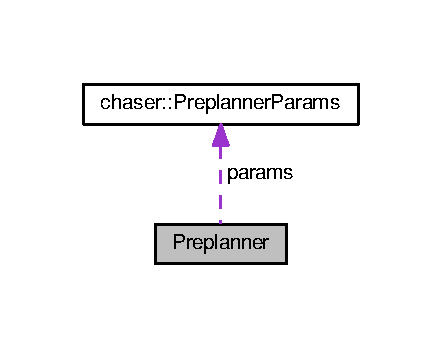
\includegraphics[width=212pt]{class_preplanner__coll__graph}
\end{center}
\end{figure}
\subsection*{Public Member Functions}
\begin{DoxyCompactItemize}
\item 
\hyperlink{class_preplanner_a4314b705278a0e3e070d5389dbb8196e}{Preplanner} ()
\item 
void \hyperlink{class_preplanner_aecde07364cbd05e2e46c95f4f5fd4951}{init} (ros\+::\+Node\+Handle nh)
\item 
void \hyperlink{class_preplanner_a6f0b709012500a44679facf0e18b985a}{preplan} (\hyperlink{struct_grid_field}{Grid\+Field} $\ast$global\+\_\+edf\+\_\+ptr, vector$<$ Point $>$ target\+\_\+pnts, Point chaser\+\_\+init)
\item 
void \hyperlink{class_preplanner_a35f3bfb85ba14d7f0c72bda1522df69e}{publish} ()
\item 
nav\+\_\+msgs\+::\+Path \hyperlink{class_preplanner_a1debbaa8e7ee64b2c22c514f89801cd1}{get\+\_\+preplanned\+\_\+waypoints} ()
\end{DoxyCompactItemize}
\subsection*{Private Member Functions}
\begin{DoxyCompactItemize}
\item 
\hyperlink{_common_8h_a225da2de31d0161f43841ed31cac064c}{Vertex\+Path} \hyperlink{class_preplanner_adff9209bb0422e7105f8bd3ed577fffd}{dijkstra} (\hyperlink{_common_8h_a1f671d518f573b692b5efa57ed576f36}{Vertex\+\_\+d} v0, \hyperlink{_common_8h_a1f671d518f573b692b5efa57ed576f36}{Vertex\+\_\+d} vf)
\item 
\hyperlink{struct_field_params}{Field\+Params} \hyperlink{class_preplanner_a5b038984427471115b1f4be24abf43b0}{get\+\_\+local\+\_\+vsf\+\_\+param\+\_\+around\+\_\+target} (Point target\+\_\+pnt)
\item 
void \hyperlink{class_preplanner_a1482068998b627fb8e2093e1eafbffd8}{compute\+\_\+visibility\+\_\+field\+\_\+seq} (\hyperlink{struct_grid_field}{Grid\+Field} $\ast$global\+\_\+edf, vector$<$ Point $>$ target\+\_\+pnts)
\item 
void \hyperlink{class_preplanner_a9404e790bfccf6563a7d947e6d11afb7}{graph\+\_\+construct} (\hyperlink{struct_grid_field}{Grid\+Field} $\ast$global\+\_\+edf, Point x0)
\item 
void \hyperlink{class_preplanner_a02321bc5136138f8aebebc494b774374}{compute\+\_\+shortest\+\_\+path} ()
\end{DoxyCompactItemize}
\subsection*{Private Attributes}
\begin{DoxyCompactItemize}
\item 
\hyperlink{structchaser_1_1_preplanner_params}{chaser\+::\+Preplanner\+Params} \hyperlink{class_preplanner_a679cc4b70f041aff73769e7ec92dc5d0}{params}
\item 
string \hyperlink{class_preplanner_a08cb79c25bd4ded139a572672e4492cd}{world\+\_\+frame\+\_\+id}
\item 
vector$<$ shared\+\_\+ptr$<$ \hyperlink{struct_grid_field}{Grid\+Field} $>$ $>$ \hyperlink{class_preplanner_aab0f91e34b86eaa581c7642ba5059308}{vsf\+\_\+field\+\_\+ptr\+\_\+seq}
\item 
\hyperlink{_common_8h_a45f376d452c699e18013842e64602733}{Graph} \hyperlink{class_preplanner_af588e8495d5e78dd5a746f7c640daa4d}{di\+\_\+graph}
\item 
\hyperlink{_common_8h_a25b10a034823d9ab576650719f0d331c}{Descriptor\+Map} \hyperlink{class_preplanner_a45603cfb24429584c4fc8bc42474e1ff}{descriptor\+\_\+map}
\item 
ros\+::\+Publisher \hyperlink{class_preplanner_a8dafcd99dc50e89404c4f33a688eba6c}{pub\+\_\+vsf\+\_\+vis}
\item 
ros\+::\+Publisher \hyperlink{class_preplanner_a9655e452a9d0e228b8c2d8cdeac8ce6b}{pub\+\_\+preplanned\+\_\+path}
\item 
ros\+::\+Publisher \hyperlink{class_preplanner_a87dc12e474ee43c9e2b095ec64ab08ce}{pub\+\_\+waypoints}
\item 
visualization\+\_\+msgs\+::\+Marker \hyperlink{class_preplanner_a9c4d6a5e43241831b0ad11bdaf99ab16}{markers\+\_\+visibility\+\_\+field\+\_\+base}
\item 
visualization\+\_\+msgs\+::\+Marker\+Array \hyperlink{class_preplanner_abcee90044b5d5935168ed132e3dfc8a6}{markers\+\_\+visibility\+\_\+field\+\_\+seq}
\item 
visualization\+\_\+msgs\+::\+Marker \hyperlink{class_preplanner_adcc96f6ec12d7cb9980aa0c889b4ccd1}{marker\+\_\+wpnts}
\item 
nav\+\_\+msgs\+::\+Path \hyperlink{class_preplanner_ace035c98e9dc23739402d346976d567b}{preplanned\+\_\+path}
\end{DoxyCompactItemize}


\subsection{Detailed Description}


\subsection{Constructor \& Destructor Documentation}
\index{Preplanner@{Preplanner}!Preplanner@{Preplanner}}
\index{Preplanner@{Preplanner}!Preplanner@{Preplanner}}
\subsubsection[{\texorpdfstring{Preplanner()}{Preplanner()}}]{\setlength{\rightskip}{0pt plus 5cm}Preplanner\+::\+Preplanner (
\begin{DoxyParamCaption}
{}
\end{DoxyParamCaption}
)}\hypertarget{class_preplanner_a4314b705278a0e3e070d5389dbb8196e}{}\label{class_preplanner_a4314b705278a0e3e070d5389dbb8196e}

\begin{DoxyCode}
3 \{\};
\end{DoxyCode}


\subsection{Member Function Documentation}
\index{Preplanner@{Preplanner}!compute\+\_\+shortest\+\_\+path@{compute\+\_\+shortest\+\_\+path}}
\index{compute\+\_\+shortest\+\_\+path@{compute\+\_\+shortest\+\_\+path}!Preplanner@{Preplanner}}
\subsubsection[{\texorpdfstring{compute\+\_\+shortest\+\_\+path()}{compute_shortest_path()}}]{\setlength{\rightskip}{0pt plus 5cm}void Preplanner\+::compute\+\_\+shortest\+\_\+path (
\begin{DoxyParamCaption}
{}
\end{DoxyParamCaption}
)\hspace{0.3cm}{\ttfamily [private]}}\hypertarget{class_preplanner_a02321bc5136138f8aebebc494b774374}{}\label{class_preplanner_a02321bc5136138f8aebebc494b774374}

\begin{DoxyCode}
303                                       \{
304 
305     ROS\_INFO(\textcolor{stringliteral}{"shortest path requested."});
306     \hyperlink{_common_8h_a225da2de31d0161f43841ed31cac064c}{VertexPath} solution\_seq = \hyperlink{class_preplanner_adff9209bb0422e7105f8bd3ed577fffd}{dijkstra}(\hyperlink{class_preplanner_a45603cfb24429584c4fc8bc42474e1ff}{descriptor\_map}[\textcolor{stringliteral}{"x0"}],
      \hyperlink{class_preplanner_a45603cfb24429584c4fc8bc42474e1ff}{descriptor\_map}[\textcolor{stringliteral}{"xf"}]);
307     \textcolor{comment}{// if path exist }
308     \textcolor{keywordflow}{if}(solution\_seq.size())\{
309 
310         solution\_seq.pop\_back();
311 
312         \textcolor{comment}{// from graph path to real path }
313         \hyperlink{class_preplanner_ace035c98e9dc23739402d346976d567b}{preplanned\_path}.poses.clear();
314         \textcolor{comment}{// marker update  }
315         \hyperlink{class_preplanner_adcc96f6ec12d7cb9980aa0c889b4ccd1}{marker\_wpnts}.points.resize(solution\_seq.size());
316         \hyperlink{class_preplanner_adcc96f6ec12d7cb9980aa0c889b4ccd1}{marker\_wpnts}.colors.resize(solution\_seq.size());  
317 
318 
319         \textcolor{keywordflow}{for}(\textcolor{keyword}{auto} it = solution\_seq.begin();it<solution\_seq.end();it++)\{
320             geometry\_msgs::PoseStamped pose\_stamped;
321 
322             pose\_stamped.pose.position = *it;
323             \hyperlink{class_preplanner_ace035c98e9dc23739402d346976d567b}{preplanned\_path}.poses.push\_back(pose\_stamped);
324 
325             \hyperlink{class_preplanner_adcc96f6ec12d7cb9980aa0c889b4ccd1}{marker\_wpnts}.colors.push\_back(\hyperlink{class_preplanner_adcc96f6ec12d7cb9980aa0c889b4ccd1}{marker\_wpnts}.color);
326             \hyperlink{class_preplanner_adcc96f6ec12d7cb9980aa0c889b4ccd1}{marker\_wpnts}.points.push\_back(*it);
327         \}
328     
329     \}
330     \textcolor{keywordflow}{else}
331         ROS\_WARN(\textcolor{stringliteral}{"[Preplanner] The preplanning couldn't be updated. (smooth planner may try to make path on
       old preplan.) "});
332     
333     
334 \}
\end{DoxyCode}
\index{Preplanner@{Preplanner}!compute\+\_\+visibility\+\_\+field\+\_\+seq@{compute\+\_\+visibility\+\_\+field\+\_\+seq}}
\index{compute\+\_\+visibility\+\_\+field\+\_\+seq@{compute\+\_\+visibility\+\_\+field\+\_\+seq}!Preplanner@{Preplanner}}
\subsubsection[{\texorpdfstring{compute\+\_\+visibility\+\_\+field\+\_\+seq(\+Grid\+Field $\ast$global\+\_\+edf, vector$<$ Point $>$ target\+\_\+pnts)}{compute_visibility_field_seq(GridField *global_edf, vector< Point > target_pnts)}}]{\setlength{\rightskip}{0pt plus 5cm}void Preplanner\+::compute\+\_\+visibility\+\_\+field\+\_\+seq (
\begin{DoxyParamCaption}
\item[{{\bf Grid\+Field} $\ast$}]{global\+\_\+edf, }
\item[{vector$<$ Point $>$}]{target\+\_\+pnts}
\end{DoxyParamCaption}
)\hspace{0.3cm}{\ttfamily [private]}}\hypertarget{class_preplanner_a1482068998b627fb8e2093e1eafbffd8}{}\label{class_preplanner_a1482068998b627fb8e2093e1eafbffd8}

\begin{DoxyCode}
92                                                                                             \{
93     \hyperlink{class_preplanner_aab0f91e34b86eaa581c7642ba5059308}{vsf\_field\_ptr\_seq}.resize(target\_pnts.size());
94     \textcolor{keywordtype}{float} numeric\_threshold = 1\hyperlink{namespace__setup__util_acdce690b925de33d6249bbbfa1109d61}{e}-2;
95     \textcolor{keywordtype}{int} t = 1;
96     \textcolor{keywordtype}{float} max\_score = -1;  \textcolor{comment}{// for visualization }
97     \textcolor{comment}{// for each target pnt}
98     \textcolor{keywordflow}{for} (\textcolor{keyword}{auto} it = target\_pnts.begin();it<target\_pnts.end();it++,t++)\{
99         
100         \textcolor{comment}{// get local conservative grid map around the current target point}
101         \textcolor{keywordtype}{int} VSF\_MODE = 1;
102         \hyperlink{class_preplanner_aab0f91e34b86eaa581c7642ba5059308}{vsf\_field\_ptr\_seq}[t-1].reset(\textcolor{keyword}{new} \hyperlink{struct_grid_field}{GridField}(
      \hyperlink{class_preplanner_a5b038984427471115b1f4be24abf43b0}{get\_local\_vsf\_param\_around\_target}(*it))); 
103         
104         \textcolor{comment}{// field value update with edf grid }
105         \textcolor{keywordflow}{for}(\textcolor{keywordtype}{int} ix = 0 ; ix<\hyperlink{class_preplanner_aab0f91e34b86eaa581c7642ba5059308}{vsf\_field\_ptr\_seq}[t-1].get()->Nx ; ix++)
106             \textcolor{keywordflow}{for}(\textcolor{keywordtype}{int} iy = 0 ; iy<\hyperlink{class_preplanner_aab0f91e34b86eaa581c7642ba5059308}{vsf\_field\_ptr\_seq}[t-1].get()->Ny ; iy++)
107                 \textcolor{keywordflow}{for}(\textcolor{keywordtype}{int} iz = 0 ; iz<\hyperlink{class_preplanner_aab0f91e34b86eaa581c7642ba5059308}{vsf\_field\_ptr\_seq}[t-1].get()->Nz ; iz++)\{
108                     
109                     \textcolor{comment}{// assign visibilty value with minimum clamping to evaluated node }
110                     Point eval\_pnt = \hyperlink{class_preplanner_aab0f91e34b86eaa581c7642ba5059308}{vsf\_field\_ptr\_seq}[t-1].get()->getCellPnt(Vector3i(ix,
      iy,iz));      
111                     \textcolor{keywordtype}{float} vs = global\_edf->\hyperlink{struct_grid_field_af9f5144af2f0cdb99784ea54c42a8516}{getRayMin}(*it,eval\_pnt,
      \hyperlink{class_preplanner_a679cc4b70f041aff73769e7ec92dc5d0}{params}.\hyperlink{structchaser_1_1_preplanner_params_a2abe7915546a5d2ebde667a1d5ccfb44}{vs\_min}); \textcolor{comment}{// visibility score from distance field                    }
112                     \hyperlink{class_preplanner_aab0f91e34b86eaa581c7642ba5059308}{vsf\_field\_ptr\_seq}[t-1].get()->field\_vals[ix][iy][iz] = vs;
113 
114                     \textcolor{comment}{// let's save the point if certain condition is satified (for graph construction)      
                }
115                     
116                     Vector3i pnt\_idx\_in\_edf = global\_edf->\hyperlink{struct_grid_field_a1a70c2de6239c1b086d01dc89b161b7c}{getCellIdx}(eval\_pnt);
117                     \textcolor{keywordtype}{float} edf\_val = global\_edf->\hyperlink{struct_grid_field_a46802a85d9533d4371d12597f0247c7d}{field\_vals}[pnt\_idx\_in\_edf(0)][pnt\_idx\_in\_edf(1)][
      pnt\_idx\_in\_edf(2)];  
118                     Vector3f bearing\_vec =(\hyperlink{_common_8h_a3e35de4eb7396984c2c5018768885d91}{geo2eigen}(eval\_pnt) - 
      \hyperlink{_common_8h_a3e35de4eb7396984c2c5018768885d91}{geo2eigen}(*it)); 
119                     \textcolor{keywordtype}{float} relative\_dist = bearing\_vec.norm();                      
120                     \textcolor{keywordtype}{float} azim = atan2(bearing\_vec(2),Vector2f(bearing\_vec(0),bearing\_vec(1)).norm());
121                     
122                     \textcolor{keywordflow}{if}(edf\_val > \hyperlink{class_preplanner_a679cc4b70f041aff73769e7ec92dc5d0}{params}.\hyperlink{structchaser_1_1_preplanner_params_a409be3b01b1b4853919d5b34e529c49a}{r\_safe} && \textcolor{comment}{// safe }
123                         relative\_dist > \hyperlink{class_preplanner_a679cc4b70f041aff73769e7ec92dc5d0}{params}.\hyperlink{structchaser_1_1_preplanner_params_aeef51c9ac61b5fa70c853463a27ff879}{d\_trakcing\_min} && \textcolor{comment}{// tracking spec}
124                         relative\_dist < \hyperlink{class_preplanner_a679cc4b70f041aff73769e7ec92dc5d0}{params}.\hyperlink{structchaser_1_1_preplanner_params_ad6659842d3039da7b064532a090651d3}{d\_trakcing\_max} && \textcolor{comment}{// tracking spec}
125                         vs > \hyperlink{class_preplanner_a679cc4b70f041aff73769e7ec92dc5d0}{params}.\hyperlink{structchaser_1_1_preplanner_params_a2abe7915546a5d2ebde667a1d5ccfb44}{vs\_min} + numeric\_threshold  && \textcolor{comment}{// non-occlusion}
126                         azim < \hyperlink{class_preplanner_a679cc4b70f041aff73769e7ec92dc5d0}{params}.\hyperlink{structchaser_1_1_preplanner_params_ab357e30646928070cd553ccf14be0beb}{max\_azim})  \textcolor{comment}{// tracking spec }
127                         \textcolor{comment}{// save}
128                         \hyperlink{class_preplanner_aab0f91e34b86eaa581c7642ba5059308}{vsf\_field\_ptr\_seq}[t-1].get()->saved\_points.push\_back(eval\_pnt);
129                     
130                     \textcolor{keywordflow}{if} (vs >= max\_score)
131                         max\_score = vs;
132 
133                 \}
134         std::cout<<\textcolor{stringliteral}{"[Preplanner] nodes at time "}<<t<<\textcolor{stringliteral}{" are "}<<\hyperlink{class_preplanner_aab0f91e34b86eaa581c7642ba5059308}{vsf\_field\_ptr\_seq}[t-1].get()
      ->saved\_points.size()<<std::endl;
135     \}
136 
137     \textcolor{comment}{// save the markers}
138 
139     \textcolor{comment}{// marker initialization     }
140     \hyperlink{class_preplanner_abcee90044b5d5935168ed132e3dfc8a6}{markers\_visibility\_field\_seq}.markers.clear();    
141 
142     \hyperlink{class_preplanner_a9c4d6a5e43241831b0ad11bdaf99ab16}{markers\_visibility\_field\_base}.header.stamp = ros::Time::now();
143     \hyperlink{class_preplanner_a9c4d6a5e43241831b0ad11bdaf99ab16}{markers\_visibility\_field\_base}.header.frame\_id = 
      \hyperlink{class_preplanner_a08cb79c25bd4ded139a572672e4492cd}{world\_frame\_id};
144     \hyperlink{class_preplanner_a9c4d6a5e43241831b0ad11bdaf99ab16}{markers\_visibility\_field\_base}.points.clear();
145     \hyperlink{class_preplanner_a9c4d6a5e43241831b0ad11bdaf99ab16}{markers\_visibility\_field\_base}.colors.clear();
146     t = 1;
147 
148     \textcolor{keywordflow}{for} (\textcolor{keyword}{auto} it = target\_pnts.begin();it<target\_pnts.end();it++,t++)\{ \textcolor{comment}{// for time}
149         \textcolor{keywordtype}{int} idx = 0;
150         \hyperlink{class_preplanner_a9c4d6a5e43241831b0ad11bdaf99ab16}{markers\_visibility\_field\_base}.ns = \textcolor{stringliteral}{"time\_"}+to\_string(t);
151 
152         \textcolor{comment}{// we draw only saved points from above }
153         \textcolor{keywordflow}{for} (\textcolor{keyword}{auto} it\_node = \hyperlink{class_preplanner_aab0f91e34b86eaa581c7642ba5059308}{vsf\_field\_ptr\_seq}[t-1].\textcolor{keyword}{get}()->saved\_points.begin() ; it\_node <
       \hyperlink{class_preplanner_aab0f91e34b86eaa581c7642ba5059308}{vsf\_field\_ptr\_seq}[t-1].get()->saved\_points.end() ; it\_node++,idx++)\{
154             Vector3i key = \hyperlink{class_preplanner_aab0f91e34b86eaa581c7642ba5059308}{vsf\_field\_ptr\_seq}[t-1].get()->getCellIdx(*it\_node);
155             \textcolor{keywordtype}{float} vs = \hyperlink{class_preplanner_aab0f91e34b86eaa581c7642ba5059308}{vsf\_field\_ptr\_seq}[t-1].get()->field\_vals[key(0)][key(1)][key(2)];
156             \textcolor{comment}{// std::cout<<vs<<std::endl;}
157             \textcolor{comment}{// marker update}
158             std\_msgs::ColorRGBA color;
159             \hyperlink{_common_8h_a75aaebf1a8b822524cc6af51a0cd83ef}{get\_color}((vs-\hyperlink{class_preplanner_a679cc4b70f041aff73769e7ec92dc5d0}{params}.\hyperlink{structchaser_1_1_preplanner_params_a2abe7915546a5d2ebde667a1d5ccfb44}{vs\_min})/(max\_score-\hyperlink{class_preplanner_a679cc4b70f041aff73769e7ec92dc5d0}{params}.
      \hyperlink{structchaser_1_1_preplanner_params_a2abe7915546a5d2ebde667a1d5ccfb44}{vs\_min}),color.r,color.g,color.b);            
160             color.a = 0.1;
161 
162             \hyperlink{class_preplanner_a9c4d6a5e43241831b0ad11bdaf99ab16}{markers\_visibility\_field\_base}.colors.push\_back(color);
163             \hyperlink{class_preplanner_a9c4d6a5e43241831b0ad11bdaf99ab16}{markers\_visibility\_field\_base}.points.push\_back(*it\_node);
164             idx ++;
165         \}
166 
167         \hyperlink{class_preplanner_abcee90044b5d5935168ed132e3dfc8a6}{markers\_visibility\_field\_seq}.markers.push\_back(
      \hyperlink{class_preplanner_a9c4d6a5e43241831b0ad11bdaf99ab16}{markers\_visibility\_field\_base});
168         \hyperlink{class_preplanner_a9c4d6a5e43241831b0ad11bdaf99ab16}{markers\_visibility\_field\_base}.points.clear();
169         \hyperlink{class_preplanner_a9c4d6a5e43241831b0ad11bdaf99ab16}{markers\_visibility\_field\_base}.colors.clear();
170         
171     \}
172 \}
\end{DoxyCode}
\index{Preplanner@{Preplanner}!dijkstra@{dijkstra}}
\index{dijkstra@{dijkstra}!Preplanner@{Preplanner}}
\subsubsection[{\texorpdfstring{dijkstra(\+Vertex\+\_\+d v0, Vertex\+\_\+d vf)}{dijkstra(Vertex_d v0, Vertex_d vf)}}]{\setlength{\rightskip}{0pt plus 5cm}{\bf Vertex\+Path} Preplanner\+::dijkstra (
\begin{DoxyParamCaption}
\item[{{\bf Vertex\+\_\+d}}]{v0, }
\item[{{\bf Vertex\+\_\+d}}]{vf}
\end{DoxyParamCaption}
)\hspace{0.3cm}{\ttfamily [private]}}\hypertarget{class_preplanner_adff9209bb0422e7105f8bd3ed577fffd}{}\label{class_preplanner_adff9209bb0422e7105f8bd3ed577fffd}

\begin{DoxyCode}
247                                                       \{
248     
249 
250 
251     \textcolor{comment}{// Create things for Dijkstra}
252     std::vector<Vertex\_d> predecessors(boost::num\_vertices(\hyperlink{class_preplanner_af588e8495d5e78dd5a746f7c640daa4d}{di\_graph})); \textcolor{comment}{// To store parents}
253     std::vector<Weight> distances(boost::num\_vertices(\hyperlink{class_preplanner_af588e8495d5e78dd5a746f7c640daa4d}{di\_graph})); \textcolor{comment}{// To store distances}
254 
255     \hyperlink{_common_8h_a7fb6309a04472de0c8cb8c74ebf92c5e}{IndexMap} indexMap = boost::get(boost::vertex\_index, \hyperlink{class_preplanner_af588e8495d5e78dd5a746f7c640daa4d}{di\_graph});
256     \hyperlink{_common_8h_a7a347729377841627777cbe0a6becbf9}{NameMap} nameMap = boost::get(boost::vertex\_name, \hyperlink{class_preplanner_af588e8495d5e78dd5a746f7c640daa4d}{di\_graph});
257 
258     \hyperlink{_common_8h_a3e372f12838999c89bb6fafe2c9b4363}{PredecessorMap} predecessorMap(&predecessors[0], indexMap);
259     \hyperlink{_common_8h_acab893c91ba1c4e4415b652ccebeea6a}{DistanceMap} distanceMap(&distances[0], indexMap);    
260 
261     boost::dijkstra\_shortest\_paths(\hyperlink{class_preplanner_af588e8495d5e78dd5a746f7c640daa4d}{di\_graph}, v0, boost::distance\_map(distanceMap).predecessor\_map(
      predecessorMap));
262 
263     \textcolor{keyword}{typedef} std::vector<Graph::edge\_descriptor> PathType;
264 
265     PathType path;
266     \hyperlink{_common_8h_a1f671d518f573b692b5efa57ed576f36}{Vertex\_d} v = vf; \textcolor{comment}{// We want to start at the destination and work our way back to the source}
267     \textcolor{keywordflow}{for}(\hyperlink{_common_8h_a1f671d518f573b692b5efa57ed576f36}{Vertex\_d} u = predecessorMap[v]; \textcolor{comment}{// Start by setting 'u' to the destintaion node's
       predecessor}
268         u != v; \textcolor{comment}{// Keep tracking the path until we get to the source}
269         v = u, u = predecessorMap[v]) \textcolor{comment}{// Set the current vertex to the current predecessor, and the
       predecessor to one level up}
270     \{
271         std::pair<Graph::edge\_descriptor, bool> edgePair = boost::edge(u, v, 
      \hyperlink{class_preplanner_af588e8495d5e78dd5a746f7c640daa4d}{di\_graph});
272         Graph::edge\_descriptor edge = edgePair.first;
273 
274         path.push\_back( edge );
275     \}
276 
277     \textcolor{keywordflow}{if} (path.size())
278     \{
279        ROS\_INFO(\textcolor{stringliteral}{"path exist"});
280         \textcolor{comment}{// Write shortest path}
281         \textcolor{keywordtype}{float} totalDistance = 0;
282 
283         \hyperlink{_common_8h_a225da2de31d0161f43841ed31cac064c}{VertexPath} vertex\_path1;
284         \hyperlink{_common_8h_a225da2de31d0161f43841ed31cac064c}{VertexPath} vertex\_path2;
285         \textcolor{keywordflow}{for}(PathType::reverse\_iterator pathIterator = path.rbegin(); pathIterator != path.rend(); ++
      pathIterator)
286         \{
287 
288 \textcolor{comment}{//            ROS\_INFO("path insertion");}
289             vertex\_path1.push\_back(nameMap[boost::source(*pathIterator, \hyperlink{class_preplanner_af588e8495d5e78dd5a746f7c640daa4d}{di\_graph})]);
290             vertex\_path2.push\_back(nameMap[boost::target(*pathIterator, \hyperlink{class_preplanner_af588e8495d5e78dd5a746f7c640daa4d}{di\_graph})]);
291         \}
292 
293         vertex\_path1.push\_back(vertex\_path2.back());
294         \textcolor{keywordflow}{return} vertex\_path1;
295     \}
296     \textcolor{keywordflow}{else}\{
297         ROS\_WARN(\textcolor{stringliteral}{"[Preplanner] path does not exist. returning zero length path. "});
298         \textcolor{keywordflow}{return} \hyperlink{_common_8h_a225da2de31d0161f43841ed31cac064c}{VertexPath}();
299     \}    
300 \}
\end{DoxyCode}
\index{Preplanner@{Preplanner}!get\+\_\+local\+\_\+vsf\+\_\+param\+\_\+around\+\_\+target@{get\+\_\+local\+\_\+vsf\+\_\+param\+\_\+around\+\_\+target}}
\index{get\+\_\+local\+\_\+vsf\+\_\+param\+\_\+around\+\_\+target@{get\+\_\+local\+\_\+vsf\+\_\+param\+\_\+around\+\_\+target}!Preplanner@{Preplanner}}
\subsubsection[{\texorpdfstring{get\+\_\+local\+\_\+vsf\+\_\+param\+\_\+around\+\_\+target(\+Point target\+\_\+pnt)}{get_local_vsf_param_around_target(Point target_pnt)}}]{\setlength{\rightskip}{0pt plus 5cm}{\bf Field\+Params} Preplanner\+::get\+\_\+local\+\_\+vsf\+\_\+param\+\_\+around\+\_\+target (
\begin{DoxyParamCaption}
\item[{Point}]{target\+\_\+pnt}
\end{DoxyParamCaption}
)\hspace{0.3cm}{\ttfamily [private]}}\hypertarget{class_preplanner_a5b038984427471115b1f4be24abf43b0}{}\label{class_preplanner_a5b038984427471115b1f4be24abf43b0}

\begin{DoxyCode}
70                                                                          \{
71 
72     \hyperlink{struct_field_params}{FieldParams} vsf\_param;    
73     \textcolor{keywordtype}{double} lx,ly,lz;
74     \textcolor{comment}{// lx = ly = 2*params.d\_trakcing\_max * cos(params.max\_azim);}
75     lx = ly = 4*\hyperlink{class_preplanner_a679cc4b70f041aff73769e7ec92dc5d0}{params}.\hyperlink{structchaser_1_1_preplanner_params_ad6659842d3039da7b064532a090651d3}{d\_trakcing\_max} ;
76     lz = \hyperlink{class_preplanner_a679cc4b70f041aff73769e7ec92dc5d0}{params}.\hyperlink{structchaser_1_1_preplanner_params_ad6659842d3039da7b064532a090651d3}{d\_trakcing\_max} * sin(\hyperlink{class_preplanner_a679cc4b70f041aff73769e7ec92dc5d0}{params}.\hyperlink{structchaser_1_1_preplanner_params_ab357e30646928070cd553ccf14be0beb}{max\_azim}) - 
      \hyperlink{class_preplanner_a679cc4b70f041aff73769e7ec92dc5d0}{params}.\hyperlink{structchaser_1_1_preplanner_params_aeef51c9ac61b5fa70c853463a27ff879}{d\_trakcing\_min} * sin(\hyperlink{class_preplanner_a679cc4b70f041aff73769e7ec92dc5d0}{params}.\hyperlink{structchaser_1_1_preplanner_params_aa6846dd2e2d69d5f0d5a9b30710db6e1}{min\_azim}) ;
77 
78     vsf\_param.\hyperlink{struct_field_params_ae702824fca4d3a4b4bbf4ac90084e3a7}{x0} = target\_pnt.x - lx/2;
79     vsf\_param.\hyperlink{struct_field_params_ae9d400dadcfaaff44706adae06664c83}{y0} = target\_pnt.y - ly/2;
80     vsf\_param.\hyperlink{struct_field_params_a51178f64cc93a37d6d8f774228c24a0f}{z0} = target\_pnt.z;
81     vsf\_param.\hyperlink{struct_field_params_a9738077907a76512e49cb284ee3f1949}{lx} = lx;
82     vsf\_param.\hyperlink{struct_field_params_afb39ded77b5714992e9b2f8c5d735d30}{ly} = ly;
83     vsf\_param.\hyperlink{struct_field_params_ae7532b58aed59f5b47233e57b67acc1a}{lz} = lz;
84     
85     vsf\_param.\hyperlink{struct_field_params_a520406c76b3abf392401626bc2161370}{resolution} = \hyperlink{class_preplanner_a679cc4b70f041aff73769e7ec92dc5d0}{params}.\hyperlink{structchaser_1_1_preplanner_params_ac30a8ee32bae78f84b863234853f6497}{vsf\_resolution};
86     vsf\_param.\hyperlink{struct_field_params_ae6eabaa6e593c9dbac48b2f96bea80ec}{ray\_stride\_res} =  \hyperlink{class_preplanner_a679cc4b70f041aff73769e7ec92dc5d0}{params}.\hyperlink{structchaser_1_1_preplanner_params_ac30a8ee32bae78f84b863234853f6497}{vsf\_resolution}; \textcolor{comment}{// not used for
       vsf grid }
87 
88     \textcolor{keywordflow}{return} vsf\_param;
89 \};
\end{DoxyCode}
\index{Preplanner@{Preplanner}!get\+\_\+preplanned\+\_\+waypoints@{get\+\_\+preplanned\+\_\+waypoints}}
\index{get\+\_\+preplanned\+\_\+waypoints@{get\+\_\+preplanned\+\_\+waypoints}!Preplanner@{Preplanner}}
\subsubsection[{\texorpdfstring{get\+\_\+preplanned\+\_\+waypoints()}{get_preplanned_waypoints()}}]{\setlength{\rightskip}{0pt plus 5cm}nav\+\_\+msgs\+::\+Path Preplanner\+::get\+\_\+preplanned\+\_\+waypoints (
\begin{DoxyParamCaption}
{}
\end{DoxyParamCaption}
)}\hypertarget{class_preplanner_a1debbaa8e7ee64b2c22c514f89801cd1}{}\label{class_preplanner_a1debbaa8e7ee64b2c22c514f89801cd1}

\begin{DoxyCode}
350 \{\textcolor{keywordflow}{return} \hyperlink{class_preplanner_ace035c98e9dc23739402d346976d567b}{preplanned\_path};\}
\end{DoxyCode}
\index{Preplanner@{Preplanner}!graph\+\_\+construct@{graph\+\_\+construct}}
\index{graph\+\_\+construct@{graph\+\_\+construct}!Preplanner@{Preplanner}}
\subsubsection[{\texorpdfstring{graph\+\_\+construct(\+Grid\+Field $\ast$global\+\_\+edf, Point x0)}{graph_construct(GridField *global_edf, Point x0)}}]{\setlength{\rightskip}{0pt plus 5cm}void Preplanner\+::graph\+\_\+construct (
\begin{DoxyParamCaption}
\item[{{\bf Grid\+Field} $\ast$}]{global\+\_\+edf, }
\item[{Point}]{x0}
\end{DoxyParamCaption}
)\hspace{0.3cm}{\ttfamily [private]}}\hypertarget{class_preplanner_a9404e790bfccf6563a7d947e6d11afb7}{}\label{class_preplanner_a9404e790bfccf6563a7d947e6d11afb7}

\begin{DoxyCode}
175                                                               \{
176     
177     \textcolor{comment}{// init graph with the initial position of chaser }
178     \hyperlink{class_preplanner_af588e8495d5e78dd5a746f7c640daa4d}{di\_graph} = \hyperlink{_common_8h_a45f376d452c699e18013842e64602733}{Graph}();
179     \hyperlink{class_preplanner_a45603cfb24429584c4fc8bc42474e1ff}{descriptor\_map}.clear();
180     
181     vector<Node<Point>> prev\_layer;
182     \hyperlink{struct_node}{Node<Point>} initial\_node; initial\_node.\hyperlink{struct_node_a01b9071c0de774c720b64583262d1559}{value} = x0; initial\_node.
      \hyperlink{struct_node_a795bdc93cbf63ccddcdf2168d858492c}{name} = \textcolor{stringliteral}{"x0"};
183     prev\_layer.push\_back(initial\_node);
184     
185     \hyperlink{_common_8h_a1f671d518f573b692b5efa57ed576f36}{Vertex\_d} v0 = boost::add\_vertex(x0,\hyperlink{class_preplanner_af588e8495d5e78dd5a746f7c640daa4d}{di\_graph});
186     \hyperlink{class_preplanner_a45603cfb24429584c4fc8bc42474e1ff}{descriptor\_map}.insert(make\_pair(\hyperlink{_common_8h_a817e52d0171d1503034d4cbe7fd89a1b}{VertexName}(\textcolor{stringliteral}{"x0"}),v0));
187  
188     \textcolor{keywordtype}{int} H = \hyperlink{class_preplanner_aab0f91e34b86eaa581c7642ba5059308}{vsf\_field\_ptr\_seq}.size(); \textcolor{comment}{// total prediction horizon }
189     \textcolor{keywordtype}{int} N\_edge = 0; 
190     \textcolor{keywordtype}{int} N\_edge\_sub = 0;
191 
192     \textcolor{comment}{// in case of t = 0, we don't need (just current step). }
193     \textcolor{keywordflow}{for}(\textcolor{keywordtype}{int} t = 1; t<H;t++)\{
194         N\_edge\_sub = 0;
195         \hyperlink{struct_grid_field}{GridField}* cur\_vsf\_ptr = \hyperlink{class_preplanner_aab0f91e34b86eaa581c7642ba5059308}{vsf\_field\_ptr\_seq}[t].get();        
196         vector<Node<Point>> cur\_layer = cur\_vsf\_ptr->\hyperlink{struct_grid_field_acd8fd9f0893ad94aa4f20b4b4d81802a}{generate\_node}(t); \textcolor{comment}{// current layer   }
197 
198         \textcolor{keywordflow}{for} (\textcolor{keyword}{auto} it\_cur = cur\_layer.begin() ; it\_cur<cur\_layer.end(); it\_cur++)\{
199             
200             \textcolor{comment}{// step1 :  let's register the node(pnt,name) in the current layer into graph }
201             Point cur\_pnt = it\_cur->value; Vector3f cur\_vec = \hyperlink{_common_8h_a3e35de4eb7396984c2c5018768885d91}{geo2eigen}(cur\_pnt); 
202             \hyperlink{_common_8h_a1f671d518f573b692b5efa57ed576f36}{Vertex\_d} cur\_vert = boost::add\_vertex(cur\_pnt,\hyperlink{class_preplanner_af588e8495d5e78dd5a746f7c640daa4d}{di\_graph});
203             \hyperlink{class_preplanner_a45603cfb24429584c4fc8bc42474e1ff}{descriptor\_map}.insert(make\_pair(it\_cur->name,cur\_vert));
204             
205             \textcolor{comment}{// call the previous layer  }
206             \hyperlink{struct_grid_field}{GridField}* prev\_vsf\_ptr = \hyperlink{class_preplanner_aab0f91e34b86eaa581c7642ba5059308}{vsf\_field\_ptr\_seq}[t-1].get();              
                
207             
208             \textcolor{comment}{// step2 : let's connect with previous layer and add edges }
209             \textcolor{keywordflow}{for}(\textcolor{keyword}{auto} it\_prev = prev\_layer.begin(); it\_prev < prev\_layer.end();it\_prev++)\{ \textcolor{comment}{// prev\_layer }
210                 \hyperlink{_common_8h_a1f671d518f573b692b5efa57ed576f36}{Vertex\_d} prev\_vert = \hyperlink{class_preplanner_a45603cfb24429584c4fc8bc42474e1ff}{descriptor\_map}[it\_prev->name];
211                 Point prev\_pnt = it\_prev->value; Vector3f prev\_vec = \hyperlink{_common_8h_a3e35de4eb7396984c2c5018768885d91}{geo2eigen}(prev\_pnt);
212 
213                 \textcolor{comment}{// this condition should be satisfied to be connected }
214                 \textcolor{keywordflow}{if}(((cur\_vec-prev\_vec).norm() < \hyperlink{class_preplanner_a679cc4b70f041aff73769e7ec92dc5d0}{params}.\hyperlink{structchaser_1_1_preplanner_params_a90021bd30b7e88b50cf9317ff3673482}{d\_connect\_max}) && (global\_edf->
      \hyperlink{struct_grid_field_af9f5144af2f0cdb99784ea54c42a8516}{getRayMin}(cur\_pnt,prev\_pnt,0) > \hyperlink{class_preplanner_a679cc4b70f041aff73769e7ec92dc5d0}{params}.\hyperlink{structchaser_1_1_preplanner_params_a409be3b01b1b4853919d5b34e529c49a}{r\_safe}) )\{
215                     \textcolor{keywordtype}{float} weight = (cur\_vec-prev\_vec).norm() + 
216                             \hyperlink{class_preplanner_a679cc4b70f041aff73769e7ec92dc5d0}{params}.\hyperlink{structchaser_1_1_preplanner_params_a1778793e5b16806c867291c1a5471a04}{w\_v}*1/sqrt(cur\_vsf\_ptr->\hyperlink{struct_grid_field_a3e49ca50129cb18db833bd4168c5d254}{getRayMean}(cur\_pnt,prev\_pnt) 
      * prev\_vsf\_ptr->\hyperlink{struct_grid_field_a3e49ca50129cb18db833bd4168c5d254}{getRayMean}(prev\_pnt,cur\_pnt)) 
217                             + \hyperlink{class_preplanner_a679cc4b70f041aff73769e7ec92dc5d0}{params}.\hyperlink{structchaser_1_1_preplanner_params_ae443edaa7e2912a6a7643272305c91f5}{w\_d}*abs((\hyperlink{_common_8h_a3e35de4eb7396984c2c5018768885d91}{geo2eigen}(cur\_vsf\_ptr->
      \hyperlink{struct_grid_field_aacd39f9388090694e5c428cc612fd887}{getCentre}()) - cur\_vec).norm() - \hyperlink{class_preplanner_a679cc4b70f041aff73769e7ec92dc5d0}{params}.\hyperlink{structchaser_1_1_preplanner_params_a6a950244cbb256abb9a4e93388c0177f}{d\_trakcing\_des});                     
218                     boost::add\_edge(prev\_vert,cur\_vert,weight,\hyperlink{class_preplanner_af588e8495d5e78dd5a746f7c640daa4d}{di\_graph});
219                     \textcolor{keywordflow}{if}(weight <1\hyperlink{namespace__setup__util_acdce690b925de33d6249bbbfa1109d61}{e}-4)
220                         ROS\_WARN(\textcolor{stringliteral}{"weight is zero"});
221                     N\_edge ++;
222                     N\_edge\_sub++;
223                 \}
224             \}            
225         \}
226         prev\_layer = cur\_layer;
227         cout<<\textcolor{stringliteral}{"[Preplanner] connected edge to this layer: "}<<N\_edge\_sub<<std::endl;
228     \}
229     
230     cout<<\textcolor{stringliteral}{"[Preplanner] total number of edges "}<<N\_edge<<std::endl;
231 
232 
233     \textcolor{comment}{// graph finishing }
234 
235     \hyperlink{struct_grid_field}{GridField}* prev\_vsf\_ptr = \hyperlink{class_preplanner_aab0f91e34b86eaa581c7642ba5059308}{vsf\_field\_ptr\_seq}[H-1].get();
236     \hyperlink{_common_8h_a1f671d518f573b692b5efa57ed576f36}{Vertex\_d} vf = boost::add\_vertex(Point(),\hyperlink{class_preplanner_af588e8495d5e78dd5a746f7c640daa4d}{di\_graph});
237     \hyperlink{class_preplanner_a45603cfb24429584c4fc8bc42474e1ff}{descriptor\_map}.insert(make\_pair(\hyperlink{_common_8h_a817e52d0171d1503034d4cbe7fd89a1b}{VertexName}(\textcolor{stringliteral}{"xf"}),vf));
238 
239     \textcolor{comment}{// step2 : let's connect with previous layer }
240     \textcolor{keywordflow}{for}(\textcolor{keyword}{auto} it\_prev = prev\_layer.begin(); it\_prev < prev\_layer.end();it\_prev++)\{ \textcolor{comment}{// prev\_layer }
241         \hyperlink{_common_8h_a1f671d518f573b692b5efa57ed576f36}{Vertex\_d} prev\_vert = \hyperlink{class_preplanner_a45603cfb24429584c4fc8bc42474e1ff}{descriptor\_map}[it\_prev->name];
242         \textcolor{comment}{// this condition should be satisfied to be connected }
243             boost::add\_edge(prev\_vert,vf,0,\hyperlink{class_preplanner_af588e8495d5e78dd5a746f7c640daa4d}{di\_graph});
244     \}
245 \}
\end{DoxyCode}
\index{Preplanner@{Preplanner}!init@{init}}
\index{init@{init}!Preplanner@{Preplanner}}
\subsubsection[{\texorpdfstring{init(ros\+::\+Node\+Handle nh)}{init(ros::NodeHandle nh)}}]{\setlength{\rightskip}{0pt plus 5cm}void Preplanner\+::init (
\begin{DoxyParamCaption}
\item[{ros\+::\+Node\+Handle}]{nh}
\end{DoxyParamCaption}
)}\hypertarget{class_preplanner_aecde07364cbd05e2e46c95f4f5fd4951}{}\label{class_preplanner_aecde07364cbd05e2e46c95f4f5fd4951}

\begin{DoxyCode}
5                                      \{
6 
7     \textcolor{comment}{// preplanner params parsing }
8     nh.param(\textcolor{stringliteral}{"w\_v"},\hyperlink{class_preplanner_a679cc4b70f041aff73769e7ec92dc5d0}{params}.\hyperlink{structchaser_1_1_preplanner_params_a1778793e5b16806c867291c1a5471a04}{w\_v},5.0);       
9     nh.param(\textcolor{stringliteral}{"w\_d"},\hyperlink{class_preplanner_a679cc4b70f041aff73769e7ec92dc5d0}{params}.\hyperlink{structchaser_1_1_preplanner_params_ae443edaa7e2912a6a7643272305c91f5}{w\_d},1.5);            
10     nh.param(\textcolor{stringliteral}{"r\_safe"},\hyperlink{class_preplanner_a679cc4b70f041aff73769e7ec92dc5d0}{params}.\hyperlink{structchaser_1_1_preplanner_params_a409be3b01b1b4853919d5b34e529c49a}{r\_safe},0.5);
11     nh.param(\textcolor{stringliteral}{"min\_z"},\hyperlink{class_preplanner_a679cc4b70f041aff73769e7ec92dc5d0}{params}.\hyperlink{structchaser_1_1_preplanner_params_ad23cd70894c614834c2a80e35de3e373}{min\_z},0.4);
12     nh.param(\textcolor{stringliteral}{"vs\_min"},\hyperlink{class_preplanner_a679cc4b70f041aff73769e7ec92dc5d0}{params}.\hyperlink{structchaser_1_1_preplanner_params_a2abe7915546a5d2ebde667a1d5ccfb44}{vs\_min},0.3);
13     nh.param(\textcolor{stringliteral}{"vsf\_resolution"},\hyperlink{class_preplanner_a679cc4b70f041aff73769e7ec92dc5d0}{params}.\hyperlink{structchaser_1_1_preplanner_params_ac30a8ee32bae78f84b863234853f6497}{vsf\_resolution},0.7);
14     nh.param(\textcolor{stringliteral}{"d\_connect\_max"},\hyperlink{class_preplanner_a679cc4b70f041aff73769e7ec92dc5d0}{params}.\hyperlink{structchaser_1_1_preplanner_params_a90021bd30b7e88b50cf9317ff3673482}{d\_connect\_max},2.5);
15 
16     nh.param(\textcolor{stringliteral}{"max\_tracking\_distance"},\hyperlink{class_preplanner_a679cc4b70f041aff73769e7ec92dc5d0}{params}.\hyperlink{structchaser_1_1_preplanner_params_ad6659842d3039da7b064532a090651d3}{d\_trakcing\_max},4.0);
17     nh.param(\textcolor{stringliteral}{"min\_tracking\_distance"},\hyperlink{class_preplanner_a679cc4b70f041aff73769e7ec92dc5d0}{params}.\hyperlink{structchaser_1_1_preplanner_params_aeef51c9ac61b5fa70c853463a27ff879}{d\_trakcing\_min},1.0);
18     nh.param(\textcolor{stringliteral}{"des\_tracking\_distance"},\hyperlink{class_preplanner_a679cc4b70f041aff73769e7ec92dc5d0}{params}.\hyperlink{structchaser_1_1_preplanner_params_a6a950244cbb256abb9a4e93388c0177f}{d\_trakcing\_des},2.5);
19     nh.param(\textcolor{stringliteral}{"max\_azim"},\hyperlink{class_preplanner_a679cc4b70f041aff73769e7ec92dc5d0}{params}.\hyperlink{structchaser_1_1_preplanner_params_ab357e30646928070cd553ccf14be0beb}{max\_azim},(3.141592/4));
20     nh.param(\textcolor{stringliteral}{"min\_azim"},\hyperlink{class_preplanner_a679cc4b70f041aff73769e7ec92dc5d0}{params}.\hyperlink{structchaser_1_1_preplanner_params_aa6846dd2e2d69d5f0d5a9b30710db6e1}{min\_azim},(3.141592/7));
21 
22 
23     \textcolor{comment}{// world\_frame\_id }
24     nh.param<\textcolor{keywordtype}{string}>(\textcolor{stringliteral}{"world\_frame\_id"},\hyperlink{class_preplanner_a08cb79c25bd4ded139a572672e4492cd}{world\_frame\_id},\textcolor{stringliteral}{"/world"});
25     nh.param<\textcolor{keywordtype}{string}>(\textcolor{stringliteral}{"world\_frame\_id"},\hyperlink{class_preplanner_a9c4d6a5e43241831b0ad11bdaf99ab16}{markers\_visibility\_field\_base}.header.
      frame\_id,\textcolor{stringliteral}{"/world"});
26     nh.param<\textcolor{keywordtype}{string}>(\textcolor{stringliteral}{"world\_frame\_id"},\hyperlink{class_preplanner_ace035c98e9dc23739402d346976d567b}{preplanned\_path}.header.frame\_id,\textcolor{stringliteral}{"/world"});
27 
28     \textcolor{comment}{// marker initialize }
29     
30     \textcolor{comment}{// waypoints }
31     \hyperlink{class_preplanner_adcc96f6ec12d7cb9980aa0c889b4ccd1}{marker\_wpnts}.header.frame\_id = \hyperlink{class_preplanner_a9c4d6a5e43241831b0ad11bdaf99ab16}{markers\_visibility\_field\_base}.
      header.frame\_id;
32     \hyperlink{class_preplanner_adcc96f6ec12d7cb9980aa0c889b4ccd1}{marker\_wpnts}.ns = \textcolor{stringliteral}{"waypoints"};
33     \hyperlink{class_preplanner_adcc96f6ec12d7cb9980aa0c889b4ccd1}{marker\_wpnts}.id = 0;
34     \hyperlink{class_preplanner_adcc96f6ec12d7cb9980aa0c889b4ccd1}{marker\_wpnts}.type = visualization\_msgs::Marker::SPHERE\_LIST;
35     \hyperlink{class_preplanner_adcc96f6ec12d7cb9980aa0c889b4ccd1}{marker\_wpnts}.color.r = 14.0/255.0;
36     \hyperlink{class_preplanner_adcc96f6ec12d7cb9980aa0c889b4ccd1}{marker\_wpnts}.color.g = 50.0/255.0;
37     \hyperlink{class_preplanner_adcc96f6ec12d7cb9980aa0c889b4ccd1}{marker\_wpnts}.color.b = 1.0;
38     \hyperlink{class_preplanner_adcc96f6ec12d7cb9980aa0c889b4ccd1}{marker\_wpnts}.color.a = 0.3;
39     \hyperlink{class_preplanner_adcc96f6ec12d7cb9980aa0c889b4ccd1}{marker\_wpnts}.pose.orientation.w = 1.0;
40     \textcolor{keywordtype}{double} scale = 0.08; 
41     \hyperlink{class_preplanner_adcc96f6ec12d7cb9980aa0c889b4ccd1}{marker\_wpnts}.scale.x = scale;
42     \hyperlink{class_preplanner_adcc96f6ec12d7cb9980aa0c889b4ccd1}{marker\_wpnts}.scale.y = scale;
43     \hyperlink{class_preplanner_adcc96f6ec12d7cb9980aa0c889b4ccd1}{marker\_wpnts}.scale.z = scale;    
44 
45     \textcolor{comment}{// vsf\_grid\_seq }
46 
47     \textcolor{comment}{// marker base}
48     visualization\_msgs::Marker marker;
49     marker.header.frame\_id = \hyperlink{class_preplanner_a9c4d6a5e43241831b0ad11bdaf99ab16}{markers\_visibility\_field\_base}.header.frame\_id;;
50     marker.action = visualization\_msgs::Marker::ADD;
51     marker.type = visualization\_msgs::Marker::CUBE\_LIST;      
52     marker.pose.orientation.x = 0;
53     marker.pose.orientation.y = 0;
54     marker.pose.orientation.z = 0;
55     marker.pose.orientation.w = 1;                  
56     marker.scale.x = \hyperlink{class_preplanner_a679cc4b70f041aff73769e7ec92dc5d0}{params}.\hyperlink{structchaser_1_1_preplanner_params_ac30a8ee32bae78f84b863234853f6497}{vsf\_resolution};
57     marker.scale.y = \hyperlink{class_preplanner_a679cc4b70f041aff73769e7ec92dc5d0}{params}.\hyperlink{structchaser_1_1_preplanner_params_ac30a8ee32bae78f84b863234853f6497}{vsf\_resolution};
58     marker.scale.z = \hyperlink{class_preplanner_a679cc4b70f041aff73769e7ec92dc5d0}{params}.\hyperlink{structchaser_1_1_preplanner_params_ac30a8ee32bae78f84b863234853f6497}{vsf\_resolution};
59     \hyperlink{class_preplanner_a9c4d6a5e43241831b0ad11bdaf99ab16}{markers\_visibility\_field\_base} = marker; 
60 
61 
62     \textcolor{comment}{// ros initialize }
63     \hyperlink{class_preplanner_a8dafcd99dc50e89404c4f33a688eba6c}{pub\_vsf\_vis} = nh.advertise<visualization\_msgs::MarkerArray>(\textcolor{stringliteral}{"vsf\_grid\_seq"},1);
64     \hyperlink{class_preplanner_a87dc12e474ee43c9e2b095ec64ab08ce}{pub\_waypoints} = nh.advertise<visualization\_msgs::Marker>(\textcolor{stringliteral}{"preplanned\_waypoints"},1);    
65     \hyperlink{class_preplanner_a9655e452a9d0e228b8c2d8cdeac8ce6b}{pub\_preplanned\_path} = nh.advertise<nav\_msgs::Path>(\textcolor{stringliteral}{"preplanned\_path"},1);
66 
67 
68 \};
\end{DoxyCode}
\index{Preplanner@{Preplanner}!preplan@{preplan}}
\index{preplan@{preplan}!Preplanner@{Preplanner}}
\subsubsection[{\texorpdfstring{preplan(\+Grid\+Field $\ast$global\+\_\+edf\+\_\+ptr, vector$<$ Point $>$ target\+\_\+pnts, Point chaser\+\_\+init)}{preplan(GridField *global_edf_ptr, vector< Point > target_pnts, Point chaser_init)}}]{\setlength{\rightskip}{0pt plus 5cm}void Preplanner\+::preplan (
\begin{DoxyParamCaption}
\item[{{\bf Grid\+Field} $\ast$}]{global\+\_\+edf\+\_\+ptr, }
\item[{vector$<$ Point $>$}]{target\+\_\+pnts, }
\item[{Point}]{chaser\+\_\+init}
\end{DoxyParamCaption}
)}\hypertarget{class_preplanner_a6f0b709012500a44679facf0e18b985a}{}\label{class_preplanner_a6f0b709012500a44679facf0e18b985a}

\begin{DoxyCode}
337                                                                                          \{
338 
339 
340 
341     \textcolor{comment}{// set the height of the moving target }
342     \textcolor{keywordflow}{for}(\textcolor{keyword}{auto} it = target\_pnts.begin(); it<target\_pnts.end(); it++)
343         it->z = \hyperlink{class_preplanner_a679cc4b70f041aff73769e7ec92dc5d0}{params}.\hyperlink{structchaser_1_1_preplanner_params_ad23cd70894c614834c2a80e35de3e373}{min\_z} + 1\hyperlink{namespace__setup__util_acdce690b925de33d6249bbbfa1109d61}{e}-3;
344 
345     \hyperlink{class_preplanner_a1482068998b627fb8e2093e1eafbffd8}{compute\_visibility\_field\_seq}(global\_edf,target\_pnts);  
346     \hyperlink{class_preplanner_a9404e790bfccf6563a7d947e6d11afb7}{graph\_construct}(global\_edf,chaser\_init);        
347     \hyperlink{class_preplanner_a02321bc5136138f8aebebc494b774374}{compute\_shortest\_path}();   
348 \}
\end{DoxyCode}
\index{Preplanner@{Preplanner}!publish@{publish}}
\index{publish@{publish}!Preplanner@{Preplanner}}
\subsubsection[{\texorpdfstring{publish()}{publish()}}]{\setlength{\rightskip}{0pt plus 5cm}void Preplanner\+::publish (
\begin{DoxyParamCaption}
{}
\end{DoxyParamCaption}
)}\hypertarget{class_preplanner_a35f3bfb85ba14d7f0c72bda1522df69e}{}\label{class_preplanner_a35f3bfb85ba14d7f0c72bda1522df69e}

\begin{DoxyCode}
352                         \{
353     \textcolor{comment}{// vsf seq}
354     \hyperlink{class_preplanner_a8dafcd99dc50e89404c4f33a688eba6c}{pub\_vsf\_vis}.publish(\hyperlink{class_preplanner_abcee90044b5d5935168ed132e3dfc8a6}{markers\_visibility\_field\_seq});
355     \textcolor{comment}{// waypoints}
356     \hyperlink{class_preplanner_a87dc12e474ee43c9e2b095ec64ab08ce}{pub\_waypoints}.publish(\hyperlink{class_preplanner_adcc96f6ec12d7cb9980aa0c889b4ccd1}{marker\_wpnts});
357     \textcolor{comment}{// preplanned path }
358     \hyperlink{class_preplanner_a9655e452a9d0e228b8c2d8cdeac8ce6b}{pub\_preplanned\_path}.publish(\hyperlink{class_preplanner_ace035c98e9dc23739402d346976d567b}{preplanned\_path});
359 \}\end{DoxyCode}


\subsection{Member Data Documentation}
\index{Preplanner@{Preplanner}!descriptor\+\_\+map@{descriptor\+\_\+map}}
\index{descriptor\+\_\+map@{descriptor\+\_\+map}!Preplanner@{Preplanner}}
\subsubsection[{\texorpdfstring{descriptor\+\_\+map}{descriptor_map}}]{\setlength{\rightskip}{0pt plus 5cm}{\bf Descriptor\+Map} Preplanner\+::descriptor\+\_\+map\hspace{0.3cm}{\ttfamily [private]}}\hypertarget{class_preplanner_a45603cfb24429584c4fc8bc42474e1ff}{}\label{class_preplanner_a45603cfb24429584c4fc8bc42474e1ff}
\index{Preplanner@{Preplanner}!di\+\_\+graph@{di\+\_\+graph}}
\index{di\+\_\+graph@{di\+\_\+graph}!Preplanner@{Preplanner}}
\subsubsection[{\texorpdfstring{di\+\_\+graph}{di_graph}}]{\setlength{\rightskip}{0pt plus 5cm}{\bf Graph} Preplanner\+::di\+\_\+graph\hspace{0.3cm}{\ttfamily [private]}}\hypertarget{class_preplanner_af588e8495d5e78dd5a746f7c640daa4d}{}\label{class_preplanner_af588e8495d5e78dd5a746f7c640daa4d}
\index{Preplanner@{Preplanner}!marker\+\_\+wpnts@{marker\+\_\+wpnts}}
\index{marker\+\_\+wpnts@{marker\+\_\+wpnts}!Preplanner@{Preplanner}}
\subsubsection[{\texorpdfstring{marker\+\_\+wpnts}{marker_wpnts}}]{\setlength{\rightskip}{0pt plus 5cm}visualization\+\_\+msgs\+::\+Marker Preplanner\+::marker\+\_\+wpnts\hspace{0.3cm}{\ttfamily [private]}}\hypertarget{class_preplanner_adcc96f6ec12d7cb9980aa0c889b4ccd1}{}\label{class_preplanner_adcc96f6ec12d7cb9980aa0c889b4ccd1}
\index{Preplanner@{Preplanner}!markers\+\_\+visibility\+\_\+field\+\_\+base@{markers\+\_\+visibility\+\_\+field\+\_\+base}}
\index{markers\+\_\+visibility\+\_\+field\+\_\+base@{markers\+\_\+visibility\+\_\+field\+\_\+base}!Preplanner@{Preplanner}}
\subsubsection[{\texorpdfstring{markers\+\_\+visibility\+\_\+field\+\_\+base}{markers_visibility_field_base}}]{\setlength{\rightskip}{0pt plus 5cm}visualization\+\_\+msgs\+::\+Marker Preplanner\+::markers\+\_\+visibility\+\_\+field\+\_\+base\hspace{0.3cm}{\ttfamily [private]}}\hypertarget{class_preplanner_a9c4d6a5e43241831b0ad11bdaf99ab16}{}\label{class_preplanner_a9c4d6a5e43241831b0ad11bdaf99ab16}
\index{Preplanner@{Preplanner}!markers\+\_\+visibility\+\_\+field\+\_\+seq@{markers\+\_\+visibility\+\_\+field\+\_\+seq}}
\index{markers\+\_\+visibility\+\_\+field\+\_\+seq@{markers\+\_\+visibility\+\_\+field\+\_\+seq}!Preplanner@{Preplanner}}
\subsubsection[{\texorpdfstring{markers\+\_\+visibility\+\_\+field\+\_\+seq}{markers_visibility_field_seq}}]{\setlength{\rightskip}{0pt plus 5cm}visualization\+\_\+msgs\+::\+Marker\+Array Preplanner\+::markers\+\_\+visibility\+\_\+field\+\_\+seq\hspace{0.3cm}{\ttfamily [private]}}\hypertarget{class_preplanner_abcee90044b5d5935168ed132e3dfc8a6}{}\label{class_preplanner_abcee90044b5d5935168ed132e3dfc8a6}
\index{Preplanner@{Preplanner}!params@{params}}
\index{params@{params}!Preplanner@{Preplanner}}
\subsubsection[{\texorpdfstring{params}{params}}]{\setlength{\rightskip}{0pt plus 5cm}{\bf chaser\+::\+Preplanner\+Params} Preplanner\+::params\hspace{0.3cm}{\ttfamily [private]}}\hypertarget{class_preplanner_a679cc4b70f041aff73769e7ec92dc5d0}{}\label{class_preplanner_a679cc4b70f041aff73769e7ec92dc5d0}
\index{Preplanner@{Preplanner}!preplanned\+\_\+path@{preplanned\+\_\+path}}
\index{preplanned\+\_\+path@{preplanned\+\_\+path}!Preplanner@{Preplanner}}
\subsubsection[{\texorpdfstring{preplanned\+\_\+path}{preplanned_path}}]{\setlength{\rightskip}{0pt plus 5cm}nav\+\_\+msgs\+::\+Path Preplanner\+::preplanned\+\_\+path\hspace{0.3cm}{\ttfamily [private]}}\hypertarget{class_preplanner_ace035c98e9dc23739402d346976d567b}{}\label{class_preplanner_ace035c98e9dc23739402d346976d567b}
\index{Preplanner@{Preplanner}!pub\+\_\+preplanned\+\_\+path@{pub\+\_\+preplanned\+\_\+path}}
\index{pub\+\_\+preplanned\+\_\+path@{pub\+\_\+preplanned\+\_\+path}!Preplanner@{Preplanner}}
\subsubsection[{\texorpdfstring{pub\+\_\+preplanned\+\_\+path}{pub_preplanned_path}}]{\setlength{\rightskip}{0pt plus 5cm}ros\+::\+Publisher Preplanner\+::pub\+\_\+preplanned\+\_\+path\hspace{0.3cm}{\ttfamily [private]}}\hypertarget{class_preplanner_a9655e452a9d0e228b8c2d8cdeac8ce6b}{}\label{class_preplanner_a9655e452a9d0e228b8c2d8cdeac8ce6b}
\index{Preplanner@{Preplanner}!pub\+\_\+vsf\+\_\+vis@{pub\+\_\+vsf\+\_\+vis}}
\index{pub\+\_\+vsf\+\_\+vis@{pub\+\_\+vsf\+\_\+vis}!Preplanner@{Preplanner}}
\subsubsection[{\texorpdfstring{pub\+\_\+vsf\+\_\+vis}{pub_vsf_vis}}]{\setlength{\rightskip}{0pt plus 5cm}ros\+::\+Publisher Preplanner\+::pub\+\_\+vsf\+\_\+vis\hspace{0.3cm}{\ttfamily [private]}}\hypertarget{class_preplanner_a8dafcd99dc50e89404c4f33a688eba6c}{}\label{class_preplanner_a8dafcd99dc50e89404c4f33a688eba6c}
\index{Preplanner@{Preplanner}!pub\+\_\+waypoints@{pub\+\_\+waypoints}}
\index{pub\+\_\+waypoints@{pub\+\_\+waypoints}!Preplanner@{Preplanner}}
\subsubsection[{\texorpdfstring{pub\+\_\+waypoints}{pub_waypoints}}]{\setlength{\rightskip}{0pt plus 5cm}ros\+::\+Publisher Preplanner\+::pub\+\_\+waypoints\hspace{0.3cm}{\ttfamily [private]}}\hypertarget{class_preplanner_a87dc12e474ee43c9e2b095ec64ab08ce}{}\label{class_preplanner_a87dc12e474ee43c9e2b095ec64ab08ce}
\index{Preplanner@{Preplanner}!vsf\+\_\+field\+\_\+ptr\+\_\+seq@{vsf\+\_\+field\+\_\+ptr\+\_\+seq}}
\index{vsf\+\_\+field\+\_\+ptr\+\_\+seq@{vsf\+\_\+field\+\_\+ptr\+\_\+seq}!Preplanner@{Preplanner}}
\subsubsection[{\texorpdfstring{vsf\+\_\+field\+\_\+ptr\+\_\+seq}{vsf_field_ptr_seq}}]{\setlength{\rightskip}{0pt plus 5cm}vector$<$shared\+\_\+ptr$<${\bf Grid\+Field}$>$ $>$ Preplanner\+::vsf\+\_\+field\+\_\+ptr\+\_\+seq\hspace{0.3cm}{\ttfamily [private]}}\hypertarget{class_preplanner_aab0f91e34b86eaa581c7642ba5059308}{}\label{class_preplanner_aab0f91e34b86eaa581c7642ba5059308}
\index{Preplanner@{Preplanner}!world\+\_\+frame\+\_\+id@{world\+\_\+frame\+\_\+id}}
\index{world\+\_\+frame\+\_\+id@{world\+\_\+frame\+\_\+id}!Preplanner@{Preplanner}}
\subsubsection[{\texorpdfstring{world\+\_\+frame\+\_\+id}{world_frame_id}}]{\setlength{\rightskip}{0pt plus 5cm}string Preplanner\+::world\+\_\+frame\+\_\+id\hspace{0.3cm}{\ttfamily [private]}}\hypertarget{class_preplanner_a08cb79c25bd4ded139a572672e4492cd}{}\label{class_preplanner_a08cb79c25bd4ded139a572672e4492cd}


The documentation for this class was generated from the following files\+:\begin{DoxyCompactItemize}
\item 
include/auto\+\_\+chaser/\hyperlink{_preplanner_8h}{Preplanner.\+h}\item 
src/auto\+\_\+chaser/\hyperlink{_preplanner_8cpp}{Preplanner.\+cpp}\end{DoxyCompactItemize}

\hypertarget{structchaser_1_1_preplanner_params}{}\section{chaser\+:\+:Preplanner\+Params Struct Reference}
\label{structchaser_1_1_preplanner_params}\index{chaser\+::\+Preplanner\+Params@{chaser\+::\+Preplanner\+Params}}


{\ttfamily \#include $<$Common.\+h$>$}

\subsection*{Public Attributes}
\begin{DoxyCompactItemize}
\item 
double \hyperlink{structchaser_1_1_preplanner_params_ad6659842d3039da7b064532a090651d3}{d\+\_\+trakcing\+\_\+max}
\item 
double \hyperlink{structchaser_1_1_preplanner_params_aeef51c9ac61b5fa70c853463a27ff879}{d\+\_\+trakcing\+\_\+min}
\item 
double \hyperlink{structchaser_1_1_preplanner_params_a6a950244cbb256abb9a4e93388c0177f}{d\+\_\+trakcing\+\_\+des}
\item 
double \hyperlink{structchaser_1_1_preplanner_params_ab357e30646928070cd553ccf14be0beb}{max\+\_\+azim}
\item 
double \hyperlink{structchaser_1_1_preplanner_params_aa6846dd2e2d69d5f0d5a9b30710db6e1}{min\+\_\+azim}
\item 
double \hyperlink{structchaser_1_1_preplanner_params_a409be3b01b1b4853919d5b34e529c49a}{r\+\_\+safe}
\item 
double \hyperlink{structchaser_1_1_preplanner_params_ad23cd70894c614834c2a80e35de3e373}{min\+\_\+z}
\item 
double \hyperlink{structchaser_1_1_preplanner_params_a2abe7915546a5d2ebde667a1d5ccfb44}{vs\+\_\+min}
\item 
double \hyperlink{structchaser_1_1_preplanner_params_ac30a8ee32bae78f84b863234853f6497}{vsf\+\_\+resolution}
\item 
double \hyperlink{structchaser_1_1_preplanner_params_a90021bd30b7e88b50cf9317ff3673482}{d\+\_\+connect\+\_\+max}
\item 
double \hyperlink{structchaser_1_1_preplanner_params_ae443edaa7e2912a6a7643272305c91f5}{w\+\_\+d}
\item 
double \hyperlink{structchaser_1_1_preplanner_params_a1778793e5b16806c867291c1a5471a04}{w\+\_\+v}
\end{DoxyCompactItemize}


\subsection{Detailed Description}


\subsection{Member Data Documentation}
\index{chaser\+::\+Preplanner\+Params@{chaser\+::\+Preplanner\+Params}!d\+\_\+connect\+\_\+max@{d\+\_\+connect\+\_\+max}}
\index{d\+\_\+connect\+\_\+max@{d\+\_\+connect\+\_\+max}!chaser\+::\+Preplanner\+Params@{chaser\+::\+Preplanner\+Params}}
\subsubsection[{\texorpdfstring{d\+\_\+connect\+\_\+max}{d_connect_max}}]{\setlength{\rightskip}{0pt plus 5cm}double chaser\+::\+Preplanner\+Params\+::d\+\_\+connect\+\_\+max}\hypertarget{structchaser_1_1_preplanner_params_a90021bd30b7e88b50cf9317ff3673482}{}\label{structchaser_1_1_preplanner_params_a90021bd30b7e88b50cf9317ff3673482}
\index{chaser\+::\+Preplanner\+Params@{chaser\+::\+Preplanner\+Params}!d\+\_\+trakcing\+\_\+des@{d\+\_\+trakcing\+\_\+des}}
\index{d\+\_\+trakcing\+\_\+des@{d\+\_\+trakcing\+\_\+des}!chaser\+::\+Preplanner\+Params@{chaser\+::\+Preplanner\+Params}}
\subsubsection[{\texorpdfstring{d\+\_\+trakcing\+\_\+des}{d_trakcing_des}}]{\setlength{\rightskip}{0pt plus 5cm}double chaser\+::\+Preplanner\+Params\+::d\+\_\+trakcing\+\_\+des}\hypertarget{structchaser_1_1_preplanner_params_a6a950244cbb256abb9a4e93388c0177f}{}\label{structchaser_1_1_preplanner_params_a6a950244cbb256abb9a4e93388c0177f}
\index{chaser\+::\+Preplanner\+Params@{chaser\+::\+Preplanner\+Params}!d\+\_\+trakcing\+\_\+max@{d\+\_\+trakcing\+\_\+max}}
\index{d\+\_\+trakcing\+\_\+max@{d\+\_\+trakcing\+\_\+max}!chaser\+::\+Preplanner\+Params@{chaser\+::\+Preplanner\+Params}}
\subsubsection[{\texorpdfstring{d\+\_\+trakcing\+\_\+max}{d_trakcing_max}}]{\setlength{\rightskip}{0pt plus 5cm}double chaser\+::\+Preplanner\+Params\+::d\+\_\+trakcing\+\_\+max}\hypertarget{structchaser_1_1_preplanner_params_ad6659842d3039da7b064532a090651d3}{}\label{structchaser_1_1_preplanner_params_ad6659842d3039da7b064532a090651d3}
\index{chaser\+::\+Preplanner\+Params@{chaser\+::\+Preplanner\+Params}!d\+\_\+trakcing\+\_\+min@{d\+\_\+trakcing\+\_\+min}}
\index{d\+\_\+trakcing\+\_\+min@{d\+\_\+trakcing\+\_\+min}!chaser\+::\+Preplanner\+Params@{chaser\+::\+Preplanner\+Params}}
\subsubsection[{\texorpdfstring{d\+\_\+trakcing\+\_\+min}{d_trakcing_min}}]{\setlength{\rightskip}{0pt plus 5cm}double chaser\+::\+Preplanner\+Params\+::d\+\_\+trakcing\+\_\+min}\hypertarget{structchaser_1_1_preplanner_params_aeef51c9ac61b5fa70c853463a27ff879}{}\label{structchaser_1_1_preplanner_params_aeef51c9ac61b5fa70c853463a27ff879}
\index{chaser\+::\+Preplanner\+Params@{chaser\+::\+Preplanner\+Params}!max\+\_\+azim@{max\+\_\+azim}}
\index{max\+\_\+azim@{max\+\_\+azim}!chaser\+::\+Preplanner\+Params@{chaser\+::\+Preplanner\+Params}}
\subsubsection[{\texorpdfstring{max\+\_\+azim}{max_azim}}]{\setlength{\rightskip}{0pt plus 5cm}double chaser\+::\+Preplanner\+Params\+::max\+\_\+azim}\hypertarget{structchaser_1_1_preplanner_params_ab357e30646928070cd553ccf14be0beb}{}\label{structchaser_1_1_preplanner_params_ab357e30646928070cd553ccf14be0beb}
\index{chaser\+::\+Preplanner\+Params@{chaser\+::\+Preplanner\+Params}!min\+\_\+azim@{min\+\_\+azim}}
\index{min\+\_\+azim@{min\+\_\+azim}!chaser\+::\+Preplanner\+Params@{chaser\+::\+Preplanner\+Params}}
\subsubsection[{\texorpdfstring{min\+\_\+azim}{min_azim}}]{\setlength{\rightskip}{0pt plus 5cm}double chaser\+::\+Preplanner\+Params\+::min\+\_\+azim}\hypertarget{structchaser_1_1_preplanner_params_aa6846dd2e2d69d5f0d5a9b30710db6e1}{}\label{structchaser_1_1_preplanner_params_aa6846dd2e2d69d5f0d5a9b30710db6e1}
\index{chaser\+::\+Preplanner\+Params@{chaser\+::\+Preplanner\+Params}!min\+\_\+z@{min\+\_\+z}}
\index{min\+\_\+z@{min\+\_\+z}!chaser\+::\+Preplanner\+Params@{chaser\+::\+Preplanner\+Params}}
\subsubsection[{\texorpdfstring{min\+\_\+z}{min_z}}]{\setlength{\rightskip}{0pt plus 5cm}double chaser\+::\+Preplanner\+Params\+::min\+\_\+z}\hypertarget{structchaser_1_1_preplanner_params_ad23cd70894c614834c2a80e35de3e373}{}\label{structchaser_1_1_preplanner_params_ad23cd70894c614834c2a80e35de3e373}
\index{chaser\+::\+Preplanner\+Params@{chaser\+::\+Preplanner\+Params}!r\+\_\+safe@{r\+\_\+safe}}
\index{r\+\_\+safe@{r\+\_\+safe}!chaser\+::\+Preplanner\+Params@{chaser\+::\+Preplanner\+Params}}
\subsubsection[{\texorpdfstring{r\+\_\+safe}{r_safe}}]{\setlength{\rightskip}{0pt plus 5cm}double chaser\+::\+Preplanner\+Params\+::r\+\_\+safe}\hypertarget{structchaser_1_1_preplanner_params_a409be3b01b1b4853919d5b34e529c49a}{}\label{structchaser_1_1_preplanner_params_a409be3b01b1b4853919d5b34e529c49a}
\index{chaser\+::\+Preplanner\+Params@{chaser\+::\+Preplanner\+Params}!vs\+\_\+min@{vs\+\_\+min}}
\index{vs\+\_\+min@{vs\+\_\+min}!chaser\+::\+Preplanner\+Params@{chaser\+::\+Preplanner\+Params}}
\subsubsection[{\texorpdfstring{vs\+\_\+min}{vs_min}}]{\setlength{\rightskip}{0pt plus 5cm}double chaser\+::\+Preplanner\+Params\+::vs\+\_\+min}\hypertarget{structchaser_1_1_preplanner_params_a2abe7915546a5d2ebde667a1d5ccfb44}{}\label{structchaser_1_1_preplanner_params_a2abe7915546a5d2ebde667a1d5ccfb44}
\index{chaser\+::\+Preplanner\+Params@{chaser\+::\+Preplanner\+Params}!vsf\+\_\+resolution@{vsf\+\_\+resolution}}
\index{vsf\+\_\+resolution@{vsf\+\_\+resolution}!chaser\+::\+Preplanner\+Params@{chaser\+::\+Preplanner\+Params}}
\subsubsection[{\texorpdfstring{vsf\+\_\+resolution}{vsf_resolution}}]{\setlength{\rightskip}{0pt plus 5cm}double chaser\+::\+Preplanner\+Params\+::vsf\+\_\+resolution}\hypertarget{structchaser_1_1_preplanner_params_ac30a8ee32bae78f84b863234853f6497}{}\label{structchaser_1_1_preplanner_params_ac30a8ee32bae78f84b863234853f6497}
\index{chaser\+::\+Preplanner\+Params@{chaser\+::\+Preplanner\+Params}!w\+\_\+d@{w\+\_\+d}}
\index{w\+\_\+d@{w\+\_\+d}!chaser\+::\+Preplanner\+Params@{chaser\+::\+Preplanner\+Params}}
\subsubsection[{\texorpdfstring{w\+\_\+d}{w_d}}]{\setlength{\rightskip}{0pt plus 5cm}double chaser\+::\+Preplanner\+Params\+::w\+\_\+d}\hypertarget{structchaser_1_1_preplanner_params_ae443edaa7e2912a6a7643272305c91f5}{}\label{structchaser_1_1_preplanner_params_ae443edaa7e2912a6a7643272305c91f5}
\index{chaser\+::\+Preplanner\+Params@{chaser\+::\+Preplanner\+Params}!w\+\_\+v@{w\+\_\+v}}
\index{w\+\_\+v@{w\+\_\+v}!chaser\+::\+Preplanner\+Params@{chaser\+::\+Preplanner\+Params}}
\subsubsection[{\texorpdfstring{w\+\_\+v}{w_v}}]{\setlength{\rightskip}{0pt plus 5cm}double chaser\+::\+Preplanner\+Params\+::w\+\_\+v}\hypertarget{structchaser_1_1_preplanner_params_a1778793e5b16806c867291c1a5471a04}{}\label{structchaser_1_1_preplanner_params_a1778793e5b16806c867291c1a5471a04}


The documentation for this struct was generated from the following file\+:\begin{DoxyCompactItemize}
\item 
/home/jbs/catkin\+\_\+ws/src/traj\+\_\+gen\+\_\+vis\+\_\+developing/include/auto\+\_\+chaser/\hyperlink{_common_8h}{Common.\+h}\end{DoxyCompactItemize}

\hypertarget{class_q_node}{}\section{Q\+Node Class Reference}
\label{class_q_node}\index{Q\+Node@{Q\+Node}}


{\ttfamily \#include $<$qnode.\+h$>$}



Inheritance diagram for Q\+Node\+:\nopagebreak
\begin{figure}[H]
\begin{center}
\leavevmode
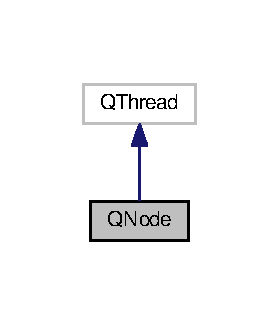
\includegraphics[width=134pt]{class_q_node__inherit__graph}
\end{center}
\end{figure}


Collaboration diagram for Q\+Node\+:
\nopagebreak
\begin{figure}[H]
\begin{center}
\leavevmode
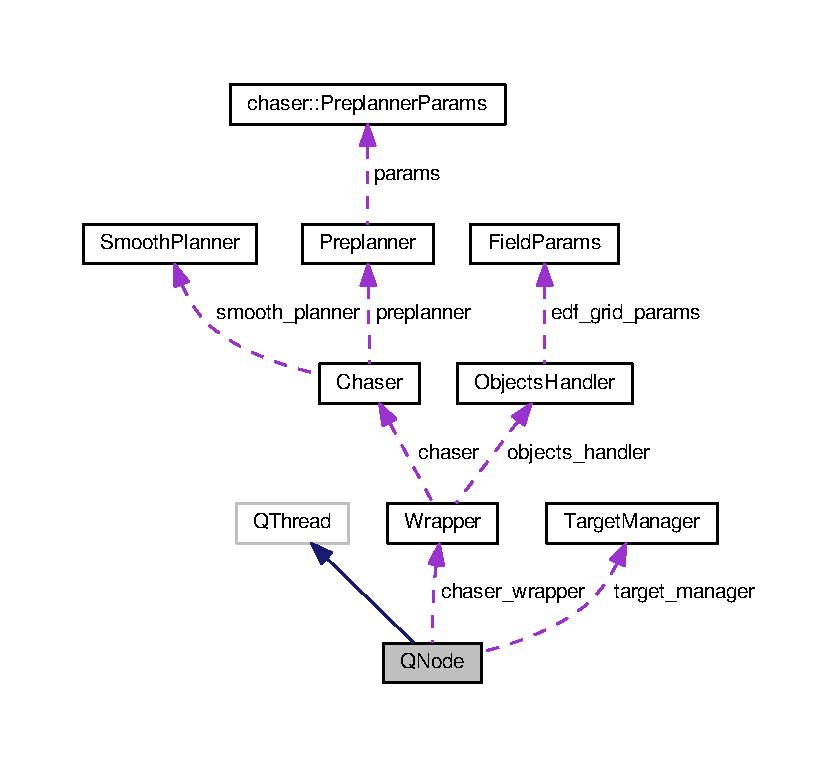
\includegraphics[width=350pt]{class_q_node__coll__graph}
\end{center}
\end{figure}
\subsection*{Signals}
\begin{DoxyCompactItemize}
\item 
void \hyperlink{class_q_node_abddcd4e0187f6d4513bbee7ba4656827}{logging\+Updated} ()
\item 
void \hyperlink{class_q_node_a7888b171c93c5f47334f5d2815adf445}{ros\+Shutdown} ()
\item 
void \hyperlink{class_q_node_a80d139522a1333db2c6ea33914c32378}{write\+On\+Board} (Q\+String)
\end{DoxyCompactItemize}
\subsection*{Public Member Functions}
\begin{DoxyCompactItemize}
\item 
\hyperlink{class_q_node_af26ee8c152283b4a1999dc5d4bd67908}{Q\+Node} (int argc, char $\ast$$\ast$argv, const std\+::string \&name)
\item 
\hyperlink{class_q_node_afed12669e9aed3e70721f507804778ca}{$\sim$\+Q\+Node} ()
\item 
bool \hyperlink{class_q_node_a32d00dbcf15c277e08caabf95af04f6e}{on\+\_\+init} ()
\item 
void \hyperlink{class_q_node_a770568addece696138f515d38408ff5c}{shutdown} ()
\item 
void \hyperlink{class_q_node_ae585b201389c51a177fa5e2fde252c84}{run} ()
\item 
bool \hyperlink{class_q_node_a65f0fc9f27f336150f33b53a7c51d80b}{trigger\+\_\+one\+\_\+shot} (double tf)
\item 
bool \hyperlink{class_q_node_a23bd7e0744ad4c7b5d5464485375bef1}{trigger} (double t\+\_\+cur)
\item 
Q\+String\+List\+Model $\ast$ \hyperlink{class_q_node_a0a6dae02f9e317488095367203fa8a58}{logging\+Model} ()
\item 
const std\+::string \& \hyperlink{class_q_node_ac21ae24311df97ac0e15c97179763b0e}{node\+Name} ()
\item 
void \hyperlink{class_q_node_a2b1b82bfd6e5e6187fe8216ba840bb09}{wpnts\+\_\+init} ()
\end{DoxyCompactItemize}
\subsection*{Public Attributes}
\begin{DoxyCompactItemize}
\item 
\hyperlink{class_target_manager}{Target\+Manager} \hyperlink{class_q_node_adc66765125dfd755d5e7f0c0eb6e6395}{target\+\_\+manager}
\item 
\hyperlink{class_wrapper}{Wrapper} \hyperlink{class_q_node_ad2d828488fb632a008c7d3ee0e1d1fa2}{chaser\+\_\+wrapper}
\item 
string \hyperlink{class_q_node_a0967d1922eeb7e39eedca309c7003d23}{write\+\_\+path}
\item 
bool \hyperlink{class_q_node_a98b08e7704b00df8648f8c08dffe950c}{is\+\_\+connected} = false
\item 
bool \hyperlink{class_q_node_a6ace2d0aa89adecfe699b3f1c3ce0b0f}{is\+\_\+in\+\_\+session} = false
\item 
bool \hyperlink{class_q_node_a9db73b60d8ffd6ac1e64ab5620f2db49}{is\+\_\+said\+\_\+edf} = false
\item 
double \hyperlink{class_q_node_a2893bbeba854c1cc89d2271804325b7b}{button\+\_\+elapsed} =0
\item 
double \hyperlink{class_q_node_ad1f3252201b932fc5d39b4f80349c7e2}{record\+\_\+dt} = 0.\+5
\item 
ros\+::\+Time \hyperlink{class_q_node_a96e6599c14732ded065ae6a5b004f872}{button\+\_\+click\+\_\+time}
\item 
double \hyperlink{class_q_node_a4b5f0a40821fbb176de620cb5a3921f7}{previous\+\_\+elapsed} = 0
\item 
double \hyperlink{class_q_node_a932e8eb11684f38ae2fb3f23639b7c70}{last\+\_\+tigger\+\_\+time} = 0
\item 
double \hyperlink{class_q_node_a7a127726e48aa5bde733d715af7a744c}{simulation\+\_\+end\+\_\+time}
\item 
double \hyperlink{class_q_node_a6e6b7e12d0d9bbc230cc9dc42a2bd087}{early\+\_\+end\+\_\+time} = 0.\+1
\item 
bool \hyperlink{class_q_node_ada91a6275708099206c452df47210045}{arrow\+\_\+record\+\_\+switch} = true
\item 
float \hyperlink{class_q_node_a3430f5db8c773c840b76794c82a9d58f}{pred\+\_\+horizon}
\item 
int \hyperlink{class_q_node_a5d5139bf1420415b2e0c2b0e52db957e}{prediction\+\_\+mode} = 0
\item 
int \hyperlink{class_q_node_aed4571afa880dc86a88b229c6517bfa1}{pred\+\_\+seq} = 4
\end{DoxyCompactItemize}
\subsection*{Protected Member Functions}
\begin{DoxyCompactItemize}
\item 
void \hyperlink{class_q_node_a498b0376fc75702fd8b61b91ef109769}{ros\+\_\+comms\+\_\+init} ()
\end{DoxyCompactItemize}
\subsection*{Protected Attributes}
\begin{DoxyCompactItemize}
\item 
int \hyperlink{class_q_node_aa0c7569195d8b9a6e568e98097f11d52}{init\+\_\+argc}
\item 
char $\ast$$\ast$ \hyperlink{class_q_node_a92c2972e3dd2a5de95d0edf8c75e1e5f}{init\+\_\+argv}
\item 
Q\+String\+List\+Model \hyperlink{class_q_node_aff2207dadd447d4c2554df19b6f7ce48}{logging}
\item 
const std\+::string \hyperlink{class_q_node_ae2a04cf101323be1e9b2be1e63a03b7f}{node\+\_\+name}
\end{DoxyCompactItemize}


\subsection{Detailed Description}


\subsection{Constructor \& Destructor Documentation}
\index{Q\+Node@{Q\+Node}!Q\+Node@{Q\+Node}}
\index{Q\+Node@{Q\+Node}!Q\+Node@{Q\+Node}}
\subsubsection[{\texorpdfstring{Q\+Node(int argc, char $\ast$$\ast$argv, const std\+::string \&name)}{QNode(int argc, char **argv, const std::string &name)}}]{\setlength{\rightskip}{0pt plus 5cm}Q\+Node\+::\+Q\+Node (
\begin{DoxyParamCaption}
\item[{int}]{argc, }
\item[{char $\ast$$\ast$}]{argv, }
\item[{const std\+::string \&}]{name}
\end{DoxyParamCaption}
)}\hypertarget{class_q_node_af26ee8c152283b4a1999dc5d4bd67908}{}\label{class_q_node_af26ee8c152283b4a1999dc5d4bd67908}

\begin{DoxyCode}
3                                                           :
4     \hyperlink{class_q_node_aa0c7569195d8b9a6e568e98097f11d52}{init\_argc}(argc),
5     \hyperlink{class_q_node_a92c2972e3dd2a5de95d0edf8c75e1e5f}{init\_argv}(argv),
6     \hyperlink{class_q_node_ae2a04cf101323be1e9b2be1e63a03b7f}{node\_name}(name)
7     \{
8         
9 \}
\end{DoxyCode}
\index{Q\+Node@{Q\+Node}!````~Q\+Node@{$\sim$\+Q\+Node}}
\index{````~Q\+Node@{$\sim$\+Q\+Node}!Q\+Node@{Q\+Node}}
\subsubsection[{\texorpdfstring{$\sim$\+Q\+Node()}{~QNode()}}]{\setlength{\rightskip}{0pt plus 5cm}Q\+Node\+::$\sim$\+Q\+Node (
\begin{DoxyParamCaption}
{}
\end{DoxyParamCaption}
)}\hypertarget{class_q_node_afed12669e9aed3e70721f507804778ca}{}\label{class_q_node_afed12669e9aed3e70721f507804778ca}

\begin{DoxyCode}
10 \{\}
\end{DoxyCode}


\subsection{Member Function Documentation}
\index{Q\+Node@{Q\+Node}!logging\+Model@{logging\+Model}}
\index{logging\+Model@{logging\+Model}!Q\+Node@{Q\+Node}}
\subsubsection[{\texorpdfstring{logging\+Model()}{loggingModel()}}]{\setlength{\rightskip}{0pt plus 5cm}Q\+String\+List\+Model$\ast$ Q\+Node\+::logging\+Model (
\begin{DoxyParamCaption}
{}
\end{DoxyParamCaption}
)\hspace{0.3cm}{\ttfamily [inline]}}\hypertarget{class_q_node_a0a6dae02f9e317488095367203fa8a58}{}\label{class_q_node_a0a6dae02f9e317488095367203fa8a58}

\begin{DoxyCode}
33 \{ \textcolor{keywordflow}{return} &\hyperlink{class_q_node_aff2207dadd447d4c2554df19b6f7ce48}{logging}; \}
\end{DoxyCode}
\index{Q\+Node@{Q\+Node}!logging\+Updated@{logging\+Updated}}
\index{logging\+Updated@{logging\+Updated}!Q\+Node@{Q\+Node}}
\subsubsection[{\texorpdfstring{logging\+Updated}{loggingUpdated}}]{\setlength{\rightskip}{0pt plus 5cm}void Q\+Node\+::logging\+Updated (
\begin{DoxyParamCaption}
{}
\end{DoxyParamCaption}
)\hspace{0.3cm}{\ttfamily [signal]}}\hypertarget{class_q_node_abddcd4e0187f6d4513bbee7ba4656827}{}\label{class_q_node_abddcd4e0187f6d4513bbee7ba4656827}
\index{Q\+Node@{Q\+Node}!node\+Name@{node\+Name}}
\index{node\+Name@{node\+Name}!Q\+Node@{Q\+Node}}
\subsubsection[{\texorpdfstring{node\+Name()}{nodeName()}}]{\setlength{\rightskip}{0pt plus 5cm}const std\+::string\& Q\+Node\+::node\+Name (
\begin{DoxyParamCaption}
{}
\end{DoxyParamCaption}
)\hspace{0.3cm}{\ttfamily [inline]}}\hypertarget{class_q_node_ac21ae24311df97ac0e15c97179763b0e}{}\label{class_q_node_ac21ae24311df97ac0e15c97179763b0e}

\begin{DoxyCode}
34 \{ \textcolor{keywordflow}{return} \hyperlink{class_q_node_ae2a04cf101323be1e9b2be1e63a03b7f}{node\_name}; \}
\end{DoxyCode}
\index{Q\+Node@{Q\+Node}!on\+\_\+init@{on\+\_\+init}}
\index{on\+\_\+init@{on\+\_\+init}!Q\+Node@{Q\+Node}}
\subsubsection[{\texorpdfstring{on\+\_\+init()}{on_init()}}]{\setlength{\rightskip}{0pt plus 5cm}bool Q\+Node\+::on\+\_\+init (
\begin{DoxyParamCaption}
{}
\end{DoxyParamCaption}
)}\hypertarget{class_q_node_a32d00dbcf15c277e08caabf95af04f6e}{}\label{class_q_node_a32d00dbcf15c277e08caabf95af04f6e}

\begin{DoxyCode}
34                    \{
35 
36     ros::init(\hyperlink{class_q_node_aa0c7569195d8b9a6e568e98097f11d52}{init\_argc},\hyperlink{class_q_node_a92c2972e3dd2a5de95d0edf8c75e1e5f}{init\_argv},\hyperlink{class_q_node_ae2a04cf101323be1e9b2be1e63a03b7f}{node\_name});
37     \textcolor{keywordflow}{if} ( ! ros::master::check() ) \{
38         \textcolor{keywordflow}{return} \textcolor{keyword}{false};
39     \}
40     ros::start(); \textcolor{comment}{// our node handles go out of scope, so we want to control shutdown explicitly.}
41     \hyperlink{class_q_node_a498b0376fc75702fd8b61b91ef109769}{ros\_comms\_init}();
42     start();
43     \textcolor{keywordflow}{return} \textcolor{keyword}{true};
44 \}
\end{DoxyCode}
\index{Q\+Node@{Q\+Node}!ros\+\_\+comms\+\_\+init@{ros\+\_\+comms\+\_\+init}}
\index{ros\+\_\+comms\+\_\+init@{ros\+\_\+comms\+\_\+init}!Q\+Node@{Q\+Node}}
\subsubsection[{\texorpdfstring{ros\+\_\+comms\+\_\+init()}{ros_comms_init()}}]{\setlength{\rightskip}{0pt plus 5cm}void Q\+Node\+::ros\+\_\+comms\+\_\+init (
\begin{DoxyParamCaption}
{}
\end{DoxyParamCaption}
)\hspace{0.3cm}{\ttfamily [protected]}}\hypertarget{class_q_node_a498b0376fc75702fd8b61b91ef109769}{}\label{class_q_node_a498b0376fc75702fd8b61b91ef109769}

\begin{DoxyCode}
11                           \{
12     
13     ros::NodeHandle nh(\textcolor{stringliteral}{"~"});
14     nh.param(\textcolor{stringliteral}{"pred\_horizon"},\hyperlink{class_q_node_a3430f5db8c773c840b76794c82a9d58f}{pred\_horizon},\textcolor{keywordtype}{float}(3.0));
15     nh.param(\textcolor{stringliteral}{"early\_end\_time"},\hyperlink{class_q_node_a6e6b7e12d0d9bbc230cc9dc42a2bd087}{early\_end\_time},0.1);
16     nh.param<\textcolor{keywordtype}{int}>(\textcolor{stringliteral}{"pred\_seq"},\hyperlink{class_q_node_aed4571afa880dc86a88b229c6517bfa1}{pred\_seq},4);
17 
18     \textcolor{comment}{// target manager init}
19     this->\hyperlink{class_q_node_adc66765125dfd755d5e7f0c0eb6e6395}{target\_manager}.\hyperlink{class_target_manager_a293bcb3b559c6e7c4ef549873791f092}{init}(nh);
20 
21     \textcolor{comment}{// wrapper init}
22     this->\hyperlink{class_q_node_ad2d828488fb632a008c7d3ee0e1d1fa2}{chaser\_wrapper}.\hyperlink{class_wrapper_af336781e7d75d525e7b152366a0e0d93}{init}(nh);
23 
24 \}
\end{DoxyCode}
\index{Q\+Node@{Q\+Node}!ros\+Shutdown@{ros\+Shutdown}}
\index{ros\+Shutdown@{ros\+Shutdown}!Q\+Node@{Q\+Node}}
\subsubsection[{\texorpdfstring{ros\+Shutdown}{rosShutdown}}]{\setlength{\rightskip}{0pt plus 5cm}void Q\+Node\+::ros\+Shutdown (
\begin{DoxyParamCaption}
{}
\end{DoxyParamCaption}
)\hspace{0.3cm}{\ttfamily [signal]}}\hypertarget{class_q_node_a7888b171c93c5f47334f5d2815adf445}{}\label{class_q_node_a7888b171c93c5f47334f5d2815adf445}
\index{Q\+Node@{Q\+Node}!run@{run}}
\index{run@{run}!Q\+Node@{Q\+Node}}
\subsubsection[{\texorpdfstring{run()}{run()}}]{\setlength{\rightskip}{0pt plus 5cm}void Q\+Node\+::run (
\begin{DoxyParamCaption}
{}
\end{DoxyParamCaption}
)}\hypertarget{class_q_node_ae585b201389c51a177fa5e2fde252c84}{}\label{class_q_node_ae585b201389c51a177fa5e2fde252c84}

\begin{DoxyCode}
46                \{
47     ros::Rate loop\_rate(50);
48     \hyperlink{class_q_node_a80d139522a1333db2c6ea33914c32378}{writeOnBoard}(\textcolor{stringliteral}{"waiting EDF computation..."});
49 
50     \textcolor{keywordflow}{while}(ros::ok())\{
51         \textcolor{keywordtype}{double} sim\_time;
52         
53         \textcolor{keywordflow}{if}(\hyperlink{class_q_node_a6ace2d0aa89adecfe699b3f1c3ce0b0f}{is\_in\_session})\{ \textcolor{comment}{// activated}
54             \textcolor{comment}{// current simulation time}
55             sim\_time = \hyperlink{class_q_node_a4b5f0a40821fbb176de620cb5a3921f7}{previous\_elapsed} + (ros::Time::now() - 
      \hyperlink{class_q_node_a96e6599c14732ded065ae6a5b004f872}{button\_click\_time}).toSec();
56             
57             \textcolor{comment}{// trigger condition }
58             \textcolor{keywordtype}{bool} trigger\_condition;
59             \textcolor{keywordflow}{if}(\hyperlink{class_q_node_a5d5139bf1420415b2e0c2b0e52db957e}{prediction\_mode} == 0)
60                 trigger\_condition = (\hyperlink{class_q_node_a932e8eb11684f38ae2fb3f23639b7c70}{last\_tigger\_time} == 0 or (sim\_time - 
      \hyperlink{class_q_node_a932e8eb11684f38ae2fb3f23639b7c70}{last\_tigger\_time}) > \hyperlink{class_q_node_a3430f5db8c773c840b76794c82a9d58f}{pred\_horizon} - \hyperlink{class_q_node_a6e6b7e12d0d9bbc230cc9dc42a2bd087}{early\_end\_time} ) and sim\_time 
      <\hyperlink{class_q_node_a7a127726e48aa5bde733d715af7a744c}{simulation\_end\_time};
61             \textcolor{keywordflow}{else} 
62                 trigger\_condition = \textcolor{keyword}{false}; \textcolor{comment}{// TODO for real prediction case }
63 
64             \textcolor{comment}{// if triggered do the followings }
65             \textcolor{keywordflow}{if}(trigger\_condition)                                
66                 \hyperlink{class_q_node_a23bd7e0744ad4c7b5d5464485375bef1}{trigger}(sim\_time);
67             
68        
69         \}\textcolor{keywordflow}{else}
70             sim\_time = \hyperlink{class_q_node_a4b5f0a40821fbb176de620cb5a3921f7}{previous\_elapsed}; 
71         
72         \textcolor{comment}{// session (publish the current information)        }
73         \hyperlink{class_q_node_adc66765125dfd755d5e7f0c0eb6e6395}{target\_manager}.\hyperlink{class_target_manager_a4af88c70bb8a0af0171ee9a49536d5c0}{session}(sim\_time);
74         \hyperlink{class_q_node_ad2d828488fb632a008c7d3ee0e1d1fa2}{chaser\_wrapper}.\hyperlink{class_wrapper_a009ee5c325926f92df42319d5469a376}{session}(sim\_time);
75         
76 
77         \textcolor{comment}{// chaser information board }
78         \textcolor{keywordflow}{if}(\hyperlink{class_q_node_ad2d828488fb632a008c7d3ee0e1d1fa2}{chaser\_wrapper}.\hyperlink{class_wrapper_a8cddd5ffbaeb5ab0b5d8d8d0c74f810f}{objects\_handler}.
      \hyperlink{class_objects_handler_acf1ef1b318defc2a39d87cea72689478}{is\_map\_recieved} and (not \hyperlink{class_q_node_a9db73b60d8ffd6ac1e64ab5620f2db49}{is\_said\_edf}))\{
79             \hyperlink{class_q_node_a80d139522a1333db2c6ea33914c32378}{writeOnBoard}(\textcolor{stringliteral}{"EDF loaded."});
80             is\_said\_edf = \textcolor{keyword}{true};
81         \}
82         
83         ros::spinOnce();
84         loop\_rate.sleep();
85     \}
86 
87 
88     Q\_EMIT \hyperlink{class_q_node_a7888b171c93c5f47334f5d2815adf445}{rosShutdown}();
89 
90 \}
\end{DoxyCode}
\index{Q\+Node@{Q\+Node}!shutdown@{shutdown}}
\index{shutdown@{shutdown}!Q\+Node@{Q\+Node}}
\subsubsection[{\texorpdfstring{shutdown()}{shutdown()}}]{\setlength{\rightskip}{0pt plus 5cm}void Q\+Node\+::shutdown (
\begin{DoxyParamCaption}
{}
\end{DoxyParamCaption}
)}\hypertarget{class_q_node_a770568addece696138f515d38408ff5c}{}\label{class_q_node_a770568addece696138f515d38408ff5c}

\begin{DoxyCode}
26                      \{
27     \textcolor{keywordflow}{if}(ros::isStarted()) \{
28       ros::shutdown(); \textcolor{comment}{// explicitly needed since we use ros::start();}
29       ros::waitForShutdown();
30     \}
31     wait();
32 \}
\end{DoxyCode}
\index{Q\+Node@{Q\+Node}!trigger@{trigger}}
\index{trigger@{trigger}!Q\+Node@{Q\+Node}}
\subsubsection[{\texorpdfstring{trigger(double t\+\_\+cur)}{trigger(double t_cur)}}]{\setlength{\rightskip}{0pt plus 5cm}bool Q\+Node\+::trigger (
\begin{DoxyParamCaption}
\item[{double}]{t\+\_\+cur}
\end{DoxyParamCaption}
)}\hypertarget{class_q_node_a23bd7e0744ad4c7b5d5464485375bef1}{}\label{class_q_node_a23bd7e0744ad4c7b5d5464485375bef1}

\begin{DoxyCode}
118                                \{
119 
120     \hyperlink{class_q_node_a932e8eb11684f38ae2fb3f23639b7c70}{last\_tigger\_time} = t\_cur;
121     VectorXd pred\_horizon\_vec(\hyperlink{class_q_node_aed4571afa880dc86a88b229c6517bfa1}{pred\_seq});
122     pred\_horizon\_vec.setLinSpaced(\hyperlink{class_q_node_aed4571afa880dc86a88b229c6517bfa1}{pred\_seq},t\_cur,t\_cur + \hyperlink{class_q_node_a3430f5db8c773c840b76794c82a9d58f}{pred\_horizon}); 
123     \textcolor{comment}{// if(t\_cur + pred\_horizon > simulation\_end\_time)\{}
124 
125     \textcolor{comment}{//     cout<<"almost there"<<endl;}
126     \textcolor{comment}{// \}}
127     \textcolor{comment}{// pred\_horizon\_vec = pred\_horizon\_vec.cwiseMin(simulation\_end\_time); // clamping with final time}
128     cout<<\textcolor{stringliteral}{"current horizon vector:\(\backslash\)n"}<<pred\_horizon\_vec<<endl; 
129     \textcolor{comment}{// we chase under this prediction }
130     vector<Point> target\_seq = \hyperlink{class_q_node_adc66765125dfd755d5e7f0c0eb6e6395}{target\_manager}.\hyperlink{class_target_manager_a63bbc724844890316a654380d0354e93}{eval\_time\_seq}(pred\_horizon\_vec);
131     
132     \textcolor{keywordflow}{if} (target\_seq.size() == 0)\{
133         this->\hyperlink{class_q_node_a80d139522a1333db2c6ea33914c32378}{writeOnBoard}(\textcolor{stringliteral}{"size of provided target sequence is zero. please generate target
       traj first."});
134         \textcolor{keywordflow}{return} \textcolor{keyword}{false};
135     \}
136     \textcolor{keywordflow}{if}(not \hyperlink{class_q_node_ad2d828488fb632a008c7d3ee0e1d1fa2}{chaser\_wrapper}.\hyperlink{class_wrapper_a8cddd5ffbaeb5ab0b5d8d8d0c74f810f}{objects\_handler}.
      \hyperlink{class_objects_handler_a16165ae7c0167ba8d2a0151a8a4fbfd5}{is\_chaser\_spawned})\{
137         this->\hyperlink{class_q_node_a80d139522a1333db2c6ea33914c32378}{writeOnBoard}(\textcolor{stringliteral}{"chaser has not been spawned."});
138         \textcolor{keywordflow}{return} \textcolor{keyword}{false};
139     \}
140 
141     \textcolor{keywordflow}{if}(not \hyperlink{class_q_node_ad2d828488fb632a008c7d3ee0e1d1fa2}{chaser\_wrapper}.\hyperlink{class_wrapper_a8cddd5ffbaeb5ab0b5d8d8d0c74f810f}{objects\_handler}.
      \hyperlink{class_objects_handler_acf1ef1b318defc2a39d87cea72689478}{is\_map\_recieved})\{
142         this->\hyperlink{class_q_node_a80d139522a1333db2c6ea33914c32378}{writeOnBoard}(\textcolor{stringliteral}{"octomap or edf has not been uploaded."});
143         \textcolor{keywordflow}{return} \textcolor{keyword}{false};
144     \}    
145 
146 
147     \textcolor{keywordflow}{return} \hyperlink{class_q_node_ad2d828488fb632a008c7d3ee0e1d1fa2}{chaser\_wrapper}.\hyperlink{class_wrapper_a21a0e115ea80e053e4f2defd1362b92f}{trigger\_chasing}(target\_seq,pred\_horizon\_vec); 
148 \}\end{DoxyCode}
\index{Q\+Node@{Q\+Node}!trigger\+\_\+one\+\_\+shot@{trigger\+\_\+one\+\_\+shot}}
\index{trigger\+\_\+one\+\_\+shot@{trigger\+\_\+one\+\_\+shot}!Q\+Node@{Q\+Node}}
\subsubsection[{\texorpdfstring{trigger\+\_\+one\+\_\+shot(double tf)}{trigger_one_shot(double tf)}}]{\setlength{\rightskip}{0pt plus 5cm}bool Q\+Node\+::trigger\+\_\+one\+\_\+shot (
\begin{DoxyParamCaption}
\item[{double}]{tf}
\end{DoxyParamCaption}
)}\hypertarget{class_q_node_a65f0fc9f27f336150f33b53a7c51d80b}{}\label{class_q_node_a65f0fc9f27f336150f33b53a7c51d80b}

\begin{DoxyCode}
92                                      \{
93     
94 
95 
96     \textcolor{comment}{// target global waypoitns  }
97     vector<Point> target\_seq = \hyperlink{_common_8h_a81915b091c29bc9aef6a74ab374f479a}{extract\_pnts\_from\_path}(
      \hyperlink{class_q_node_adc66765125dfd755d5e7f0c0eb6e6395}{target\_manager}.\hyperlink{class_target_manager_a747b82bf5cb4d1d3574dbc08a117538f}{get\_global\_waypoints}());
98     \textcolor{keywordflow}{if} (target\_seq.size() == 0)\{
99         this->\hyperlink{class_q_node_a80d139522a1333db2c6ea33914c32378}{writeOnBoard}(\textcolor{stringliteral}{"size of provided target sequence is zero. please generate target
       traj first."});
100         \textcolor{keywordflow}{return} \textcolor{keyword}{false};
101     \}
102     \textcolor{keywordflow}{if}(not \hyperlink{class_q_node_ad2d828488fb632a008c7d3ee0e1d1fa2}{chaser\_wrapper}.\hyperlink{class_wrapper_a8cddd5ffbaeb5ab0b5d8d8d0c74f810f}{objects\_handler}.
      \hyperlink{class_objects_handler_a16165ae7c0167ba8d2a0151a8a4fbfd5}{is\_chaser\_spawned})\{
103         this->\hyperlink{class_q_node_a80d139522a1333db2c6ea33914c32378}{writeOnBoard}(\textcolor{stringliteral}{"chaser has not been spawned."});
104         \textcolor{keywordflow}{return} \textcolor{keyword}{false};
105     \}
106 
107     \textcolor{keywordflow}{if}(not \hyperlink{class_q_node_ad2d828488fb632a008c7d3ee0e1d1fa2}{chaser\_wrapper}.\hyperlink{class_wrapper_a8cddd5ffbaeb5ab0b5d8d8d0c74f810f}{objects\_handler}.
      \hyperlink{class_objects_handler_acf1ef1b318defc2a39d87cea72689478}{is\_map\_recieved})\{
108         this->\hyperlink{class_q_node_a80d139522a1333db2c6ea33914c32378}{writeOnBoard}(\textcolor{stringliteral}{"octomap or edf has not been uploaded."});
109         \textcolor{keywordflow}{return} \textcolor{keyword}{false};
110     \}    
111 
112     \textcolor{comment}{// trigger chasing}
113     VectorXd knots;    
114     knots.setLinSpaced(\hyperlink{class_q_node_adc66765125dfd755d5e7f0c0eb6e6395}{target\_manager}.\hyperlink{class_target_manager_a0bbcb1981504e3bc587c3a98f41a91e9}{queue}.size(),0,tf); 
115     \textcolor{keywordtype}{bool} is\_success =  \hyperlink{class_q_node_ad2d828488fb632a008c7d3ee0e1d1fa2}{chaser\_wrapper}.\hyperlink{class_wrapper_a21a0e115ea80e053e4f2defd1362b92f}{trigger\_chasing}(target\_seq,knots);      
        
116 \}
\end{DoxyCode}
\index{Q\+Node@{Q\+Node}!wpnts\+\_\+init@{wpnts\+\_\+init}}
\index{wpnts\+\_\+init@{wpnts\+\_\+init}!Q\+Node@{Q\+Node}}
\subsubsection[{\texorpdfstring{wpnts\+\_\+init()}{wpnts_init()}}]{\setlength{\rightskip}{0pt plus 5cm}void Q\+Node\+::wpnts\+\_\+init (
\begin{DoxyParamCaption}
{}
\end{DoxyParamCaption}
)}\hypertarget{class_q_node_a2b1b82bfd6e5e6187fe8216ba840bb09}{}\label{class_q_node_a2b1b82bfd6e5e6187fe8216ba840bb09}
\index{Q\+Node@{Q\+Node}!write\+On\+Board@{write\+On\+Board}}
\index{write\+On\+Board@{write\+On\+Board}!Q\+Node@{Q\+Node}}
\subsubsection[{\texorpdfstring{write\+On\+Board}{writeOnBoard}}]{\setlength{\rightskip}{0pt plus 5cm}void Q\+Node\+::write\+On\+Board (
\begin{DoxyParamCaption}
\item[{Q\+String}]{}
\end{DoxyParamCaption}
)\hspace{0.3cm}{\ttfamily [signal]}}\hypertarget{class_q_node_a80d139522a1333db2c6ea33914c32378}{}\label{class_q_node_a80d139522a1333db2c6ea33914c32378}


\subsection{Member Data Documentation}
\index{Q\+Node@{Q\+Node}!arrow\+\_\+record\+\_\+switch@{arrow\+\_\+record\+\_\+switch}}
\index{arrow\+\_\+record\+\_\+switch@{arrow\+\_\+record\+\_\+switch}!Q\+Node@{Q\+Node}}
\subsubsection[{\texorpdfstring{arrow\+\_\+record\+\_\+switch}{arrow_record_switch}}]{\setlength{\rightskip}{0pt plus 5cm}bool Q\+Node\+::arrow\+\_\+record\+\_\+switch = true}\hypertarget{class_q_node_ada91a6275708099206c452df47210045}{}\label{class_q_node_ada91a6275708099206c452df47210045}
\index{Q\+Node@{Q\+Node}!button\+\_\+click\+\_\+time@{button\+\_\+click\+\_\+time}}
\index{button\+\_\+click\+\_\+time@{button\+\_\+click\+\_\+time}!Q\+Node@{Q\+Node}}
\subsubsection[{\texorpdfstring{button\+\_\+click\+\_\+time}{button_click_time}}]{\setlength{\rightskip}{0pt plus 5cm}ros\+::\+Time Q\+Node\+::button\+\_\+click\+\_\+time}\hypertarget{class_q_node_a96e6599c14732ded065ae6a5b004f872}{}\label{class_q_node_a96e6599c14732ded065ae6a5b004f872}
\index{Q\+Node@{Q\+Node}!button\+\_\+elapsed@{button\+\_\+elapsed}}
\index{button\+\_\+elapsed@{button\+\_\+elapsed}!Q\+Node@{Q\+Node}}
\subsubsection[{\texorpdfstring{button\+\_\+elapsed}{button_elapsed}}]{\setlength{\rightskip}{0pt plus 5cm}double Q\+Node\+::button\+\_\+elapsed =0}\hypertarget{class_q_node_a2893bbeba854c1cc89d2271804325b7b}{}\label{class_q_node_a2893bbeba854c1cc89d2271804325b7b}
\index{Q\+Node@{Q\+Node}!chaser\+\_\+wrapper@{chaser\+\_\+wrapper}}
\index{chaser\+\_\+wrapper@{chaser\+\_\+wrapper}!Q\+Node@{Q\+Node}}
\subsubsection[{\texorpdfstring{chaser\+\_\+wrapper}{chaser_wrapper}}]{\setlength{\rightskip}{0pt plus 5cm}{\bf Wrapper} Q\+Node\+::chaser\+\_\+wrapper}\hypertarget{class_q_node_ad2d828488fb632a008c7d3ee0e1d1fa2}{}\label{class_q_node_ad2d828488fb632a008c7d3ee0e1d1fa2}
\index{Q\+Node@{Q\+Node}!early\+\_\+end\+\_\+time@{early\+\_\+end\+\_\+time}}
\index{early\+\_\+end\+\_\+time@{early\+\_\+end\+\_\+time}!Q\+Node@{Q\+Node}}
\subsubsection[{\texorpdfstring{early\+\_\+end\+\_\+time}{early_end_time}}]{\setlength{\rightskip}{0pt plus 5cm}double Q\+Node\+::early\+\_\+end\+\_\+time = 0.\+1}\hypertarget{class_q_node_a6e6b7e12d0d9bbc230cc9dc42a2bd087}{}\label{class_q_node_a6e6b7e12d0d9bbc230cc9dc42a2bd087}
\index{Q\+Node@{Q\+Node}!init\+\_\+argc@{init\+\_\+argc}}
\index{init\+\_\+argc@{init\+\_\+argc}!Q\+Node@{Q\+Node}}
\subsubsection[{\texorpdfstring{init\+\_\+argc}{init_argc}}]{\setlength{\rightskip}{0pt plus 5cm}int Q\+Node\+::init\+\_\+argc\hspace{0.3cm}{\ttfamily [protected]}}\hypertarget{class_q_node_aa0c7569195d8b9a6e568e98097f11d52}{}\label{class_q_node_aa0c7569195d8b9a6e568e98097f11d52}
\index{Q\+Node@{Q\+Node}!init\+\_\+argv@{init\+\_\+argv}}
\index{init\+\_\+argv@{init\+\_\+argv}!Q\+Node@{Q\+Node}}
\subsubsection[{\texorpdfstring{init\+\_\+argv}{init_argv}}]{\setlength{\rightskip}{0pt plus 5cm}char$\ast$$\ast$ Q\+Node\+::init\+\_\+argv\hspace{0.3cm}{\ttfamily [protected]}}\hypertarget{class_q_node_a92c2972e3dd2a5de95d0edf8c75e1e5f}{}\label{class_q_node_a92c2972e3dd2a5de95d0edf8c75e1e5f}
\index{Q\+Node@{Q\+Node}!is\+\_\+connected@{is\+\_\+connected}}
\index{is\+\_\+connected@{is\+\_\+connected}!Q\+Node@{Q\+Node}}
\subsubsection[{\texorpdfstring{is\+\_\+connected}{is_connected}}]{\setlength{\rightskip}{0pt plus 5cm}bool Q\+Node\+::is\+\_\+connected = false}\hypertarget{class_q_node_a98b08e7704b00df8648f8c08dffe950c}{}\label{class_q_node_a98b08e7704b00df8648f8c08dffe950c}
\index{Q\+Node@{Q\+Node}!is\+\_\+in\+\_\+session@{is\+\_\+in\+\_\+session}}
\index{is\+\_\+in\+\_\+session@{is\+\_\+in\+\_\+session}!Q\+Node@{Q\+Node}}
\subsubsection[{\texorpdfstring{is\+\_\+in\+\_\+session}{is_in_session}}]{\setlength{\rightskip}{0pt plus 5cm}bool Q\+Node\+::is\+\_\+in\+\_\+session = false}\hypertarget{class_q_node_a6ace2d0aa89adecfe699b3f1c3ce0b0f}{}\label{class_q_node_a6ace2d0aa89adecfe699b3f1c3ce0b0f}
\index{Q\+Node@{Q\+Node}!is\+\_\+said\+\_\+edf@{is\+\_\+said\+\_\+edf}}
\index{is\+\_\+said\+\_\+edf@{is\+\_\+said\+\_\+edf}!Q\+Node@{Q\+Node}}
\subsubsection[{\texorpdfstring{is\+\_\+said\+\_\+edf}{is_said_edf}}]{\setlength{\rightskip}{0pt plus 5cm}bool Q\+Node\+::is\+\_\+said\+\_\+edf = false}\hypertarget{class_q_node_a9db73b60d8ffd6ac1e64ab5620f2db49}{}\label{class_q_node_a9db73b60d8ffd6ac1e64ab5620f2db49}
\index{Q\+Node@{Q\+Node}!last\+\_\+tigger\+\_\+time@{last\+\_\+tigger\+\_\+time}}
\index{last\+\_\+tigger\+\_\+time@{last\+\_\+tigger\+\_\+time}!Q\+Node@{Q\+Node}}
\subsubsection[{\texorpdfstring{last\+\_\+tigger\+\_\+time}{last_tigger_time}}]{\setlength{\rightskip}{0pt plus 5cm}double Q\+Node\+::last\+\_\+tigger\+\_\+time = 0}\hypertarget{class_q_node_a932e8eb11684f38ae2fb3f23639b7c70}{}\label{class_q_node_a932e8eb11684f38ae2fb3f23639b7c70}
\index{Q\+Node@{Q\+Node}!logging@{logging}}
\index{logging@{logging}!Q\+Node@{Q\+Node}}
\subsubsection[{\texorpdfstring{logging}{logging}}]{\setlength{\rightskip}{0pt plus 5cm}Q\+String\+List\+Model Q\+Node\+::logging\hspace{0.3cm}{\ttfamily [protected]}}\hypertarget{class_q_node_aff2207dadd447d4c2554df19b6f7ce48}{}\label{class_q_node_aff2207dadd447d4c2554df19b6f7ce48}
\index{Q\+Node@{Q\+Node}!node\+\_\+name@{node\+\_\+name}}
\index{node\+\_\+name@{node\+\_\+name}!Q\+Node@{Q\+Node}}
\subsubsection[{\texorpdfstring{node\+\_\+name}{node_name}}]{\setlength{\rightskip}{0pt plus 5cm}const std\+::string Q\+Node\+::node\+\_\+name\hspace{0.3cm}{\ttfamily [protected]}}\hypertarget{class_q_node_ae2a04cf101323be1e9b2be1e63a03b7f}{}\label{class_q_node_ae2a04cf101323be1e9b2be1e63a03b7f}
\index{Q\+Node@{Q\+Node}!pred\+\_\+horizon@{pred\+\_\+horizon}}
\index{pred\+\_\+horizon@{pred\+\_\+horizon}!Q\+Node@{Q\+Node}}
\subsubsection[{\texorpdfstring{pred\+\_\+horizon}{pred_horizon}}]{\setlength{\rightskip}{0pt plus 5cm}float Q\+Node\+::pred\+\_\+horizon}\hypertarget{class_q_node_a3430f5db8c773c840b76794c82a9d58f}{}\label{class_q_node_a3430f5db8c773c840b76794c82a9d58f}
\index{Q\+Node@{Q\+Node}!pred\+\_\+seq@{pred\+\_\+seq}}
\index{pred\+\_\+seq@{pred\+\_\+seq}!Q\+Node@{Q\+Node}}
\subsubsection[{\texorpdfstring{pred\+\_\+seq}{pred_seq}}]{\setlength{\rightskip}{0pt plus 5cm}int Q\+Node\+::pred\+\_\+seq = 4}\hypertarget{class_q_node_aed4571afa880dc86a88b229c6517bfa1}{}\label{class_q_node_aed4571afa880dc86a88b229c6517bfa1}
\index{Q\+Node@{Q\+Node}!prediction\+\_\+mode@{prediction\+\_\+mode}}
\index{prediction\+\_\+mode@{prediction\+\_\+mode}!Q\+Node@{Q\+Node}}
\subsubsection[{\texorpdfstring{prediction\+\_\+mode}{prediction_mode}}]{\setlength{\rightskip}{0pt plus 5cm}int Q\+Node\+::prediction\+\_\+mode = 0}\hypertarget{class_q_node_a5d5139bf1420415b2e0c2b0e52db957e}{}\label{class_q_node_a5d5139bf1420415b2e0c2b0e52db957e}
\index{Q\+Node@{Q\+Node}!previous\+\_\+elapsed@{previous\+\_\+elapsed}}
\index{previous\+\_\+elapsed@{previous\+\_\+elapsed}!Q\+Node@{Q\+Node}}
\subsubsection[{\texorpdfstring{previous\+\_\+elapsed}{previous_elapsed}}]{\setlength{\rightskip}{0pt plus 5cm}double Q\+Node\+::previous\+\_\+elapsed = 0}\hypertarget{class_q_node_a4b5f0a40821fbb176de620cb5a3921f7}{}\label{class_q_node_a4b5f0a40821fbb176de620cb5a3921f7}
\index{Q\+Node@{Q\+Node}!record\+\_\+dt@{record\+\_\+dt}}
\index{record\+\_\+dt@{record\+\_\+dt}!Q\+Node@{Q\+Node}}
\subsubsection[{\texorpdfstring{record\+\_\+dt}{record_dt}}]{\setlength{\rightskip}{0pt plus 5cm}double Q\+Node\+::record\+\_\+dt = 0.\+5}\hypertarget{class_q_node_ad1f3252201b932fc5d39b4f80349c7e2}{}\label{class_q_node_ad1f3252201b932fc5d39b4f80349c7e2}
\index{Q\+Node@{Q\+Node}!simulation\+\_\+end\+\_\+time@{simulation\+\_\+end\+\_\+time}}
\index{simulation\+\_\+end\+\_\+time@{simulation\+\_\+end\+\_\+time}!Q\+Node@{Q\+Node}}
\subsubsection[{\texorpdfstring{simulation\+\_\+end\+\_\+time}{simulation_end_time}}]{\setlength{\rightskip}{0pt plus 5cm}double Q\+Node\+::simulation\+\_\+end\+\_\+time}\hypertarget{class_q_node_a7a127726e48aa5bde733d715af7a744c}{}\label{class_q_node_a7a127726e48aa5bde733d715af7a744c}
\index{Q\+Node@{Q\+Node}!target\+\_\+manager@{target\+\_\+manager}}
\index{target\+\_\+manager@{target\+\_\+manager}!Q\+Node@{Q\+Node}}
\subsubsection[{\texorpdfstring{target\+\_\+manager}{target_manager}}]{\setlength{\rightskip}{0pt plus 5cm}{\bf Target\+Manager} Q\+Node\+::target\+\_\+manager}\hypertarget{class_q_node_adc66765125dfd755d5e7f0c0eb6e6395}{}\label{class_q_node_adc66765125dfd755d5e7f0c0eb6e6395}
\index{Q\+Node@{Q\+Node}!write\+\_\+path@{write\+\_\+path}}
\index{write\+\_\+path@{write\+\_\+path}!Q\+Node@{Q\+Node}}
\subsubsection[{\texorpdfstring{write\+\_\+path}{write_path}}]{\setlength{\rightskip}{0pt plus 5cm}string Q\+Node\+::write\+\_\+path}\hypertarget{class_q_node_a0967d1922eeb7e39eedca309c7003d23}{}\label{class_q_node_a0967d1922eeb7e39eedca309c7003d23}


The documentation for this class was generated from the following files\+:\begin{DoxyCompactItemize}
\item 
src/qt\+\_\+ui/\hyperlink{qnode_8h}{qnode.\+h}\item 
src/qt\+\_\+ui/\hyperlink{qnode_8cpp}{qnode.\+cpp}\end{DoxyCompactItemize}

\hypertarget{class_smooth_planner}{}\section{Smooth\+Planner Class Reference}
\label{class_smooth_planner}\index{Smooth\+Planner@{Smooth\+Planner}}


{\ttfamily \#include $<$Smooth\+Planner.\+h$>$}

\subsection*{Public Member Functions}
\begin{DoxyCompactItemize}
\item 
\hyperlink{class_smooth_planner_a84977f10ce3e96fac997076324ca2909}{Smooth\+Planner} ()
\item 
void \hyperlink{class_smooth_planner_a34508c873d458075880afbae0e9c933e}{init} (ros\+::\+Node\+Handle nh)
\item 
void \hyperlink{class_smooth_planner_afc03abbd5f6473f2bc952f70195326ac}{traj\+\_\+gen} (Time\+Series knots, nav\+\_\+msgs\+::\+Path waypoints, Twist v0, Twist a0)
\item 
void \hyperlink{class_smooth_planner_a2996c73522e93adff70eb68e18c55951}{publish} ()
\end{DoxyCompactItemize}
\subsection*{Public Attributes}
\begin{DoxyCompactItemize}
\item 
Path\+Planner \hyperlink{class_smooth_planner_aa9df69d4f514c7338ab2d066d38dd1a2}{planner}
\item 
Traj\+Gen\+Opts \hyperlink{class_smooth_planner_af0c954aea3c6b5b82a160ed4be93fb17}{option}
\item 
ros\+::\+Publisher \hyperlink{class_smooth_planner_a7b8400f711456291e567d0fc204c274b}{pub\+\_\+path}
\item 
ros\+::\+Publisher \hyperlink{class_smooth_planner_a7cd9de34963f445a21a6d0101346b071}{pub\+\_\+chasing\+\_\+corridor}
\item 
ros\+::\+Publisher \hyperlink{class_smooth_planner_a7ee67bceac6d60409542a2250b2ccd08}{pub\+\_\+knots}
\item 
string \hyperlink{class_smooth_planner_ade278c4209b962d8342a2ee30e718c8b}{world\+\_\+frame\+\_\+id}
\item 
visualization\+\_\+msgs\+::\+Marker \hyperlink{class_smooth_planner_addf7aab458c1407f23e3544bd76ac82b}{chasing\+\_\+corridor}
\item 
nav\+\_\+msgs\+::\+Path \hyperlink{class_smooth_planner_a6a33038c6041ff972bea7765780b56d0}{chasing\+\_\+smooth\+\_\+path}
\item 
visualization\+\_\+msgs\+::\+Marker \hyperlink{class_smooth_planner_afeeab9ce830d4960babdc84c82da94ea}{marker\+\_\+knots}
\end{DoxyCompactItemize}


\subsection{Detailed Description}


\subsection{Constructor \& Destructor Documentation}
\index{Smooth\+Planner@{Smooth\+Planner}!Smooth\+Planner@{Smooth\+Planner}}
\index{Smooth\+Planner@{Smooth\+Planner}!Smooth\+Planner@{Smooth\+Planner}}
\subsubsection[{\texorpdfstring{Smooth\+Planner()}{SmoothPlanner()}}]{\setlength{\rightskip}{0pt plus 5cm}Smooth\+Planner\+::\+Smooth\+Planner (
\begin{DoxyParamCaption}
{}
\end{DoxyParamCaption}
)}\hypertarget{class_smooth_planner_a84977f10ce3e96fac997076324ca2909}{}\label{class_smooth_planner_a84977f10ce3e96fac997076324ca2909}

\begin{DoxyCode}
3 \{\}
\end{DoxyCode}


\subsection{Member Function Documentation}
\index{Smooth\+Planner@{Smooth\+Planner}!init@{init}}
\index{init@{init}!Smooth\+Planner@{Smooth\+Planner}}
\subsubsection[{\texorpdfstring{init(ros\+::\+Node\+Handle nh)}{init(ros::NodeHandle nh)}}]{\setlength{\rightskip}{0pt plus 5cm}void Smooth\+Planner\+::init (
\begin{DoxyParamCaption}
\item[{ros\+::\+Node\+Handle}]{nh}
\end{DoxyParamCaption}
)}\hypertarget{class_smooth_planner_a34508c873d458075880afbae0e9c933e}{}\label{class_smooth_planner_a34508c873d458075880afbae0e9c933e}

\begin{DoxyCode}
5                                         \{
6 
7     \textcolor{comment}{// paramter parsing for option }
8     nh.param<\textcolor{keywordtype}{string}>(\textcolor{stringliteral}{"world\_frame\_id"},\hyperlink{class_smooth_planner_ade278c4209b962d8342a2ee30e718c8b}{world\_frame\_id},\textcolor{stringliteral}{"/world"});
9     nh.param<\textcolor{keywordtype}{double}>(\textcolor{stringliteral}{"chaser/safe\_corridor\_r"},\hyperlink{class_smooth_planner_af0c954aea3c6b5b82a160ed4be93fb17}{option}.safe\_r,0.5);
10     nh.param<\textcolor{keywordtype}{int}>(\textcolor{stringliteral}{"chaser/N\_safe\_pnts"},\hyperlink{class_smooth_planner_af0c954aea3c6b5b82a160ed4be93fb17}{option}.N\_safe\_pnts,3);
11     nh.param<\textcolor{keywordtype}{int}>(\textcolor{stringliteral}{"chaser/objective\_derivative"},\hyperlink{class_smooth_planner_af0c954aea3c6b5b82a160ed4be93fb17}{option}.objective\_derivative,3);
12     nh.param<\textcolor{keywordtype}{bool}>(\textcolor{stringliteral}{"chaser/is\_multi\_corridor"},\hyperlink{class_smooth_planner_af0c954aea3c6b5b82a160ed4be93fb17}{option}.is\_multi\_corridor,\textcolor{keyword}{true});
13     nh.param<\textcolor{keywordtype}{bool}>(\textcolor{stringliteral}{"chaser/is\_waypoint\_soft"},\hyperlink{class_smooth_planner_af0c954aea3c6b5b82a160ed4be93fb17}{option}.is\_waypoint\_soft,\textcolor{keyword}{true});
14     nh.param<\textcolor{keywordtype}{double}>(\textcolor{stringliteral}{"chaser/w\_deviation"},\hyperlink{class_smooth_planner_af0c954aea3c6b5b82a160ed4be93fb17}{option}.w\_d,0.5);
15     nh.param<\textcolor{keywordtype}{int}>(\textcolor{stringliteral}{"chaser/poly\_order"},\hyperlink{class_smooth_planner_af0c954aea3c6b5b82a160ed4be93fb17}{option}.poly\_order,6);
16     nh.param<\textcolor{keywordtype}{bool}>(\textcolor{stringliteral}{"chaser/verbose"},\hyperlink{class_smooth_planner_af0c954aea3c6b5b82a160ed4be93fb17}{option}.verbose,\textcolor{keyword}{true});
17 
18     \hyperlink{class_smooth_planner_a7cd9de34963f445a21a6d0101346b071}{pub\_chasing\_corridor} = nh.advertise<visualization\_msgs::Marker>(\textcolor{stringliteral}{"chasing\_corridor"},
      1); 
19     \hyperlink{class_smooth_planner_a7b8400f711456291e567d0fc204c274b}{pub\_path} = nh.advertise<nav\_msgs::Path>(\textcolor{stringliteral}{"smooth\_path"},1);
20     \hyperlink{class_smooth_planner_a7ee67bceac6d60409542a2250b2ccd08}{pub\_knots} = nh.advertise<visualization\_msgs::Marker>(\textcolor{stringliteral}{"smooth\_path\_knots"},1);
21 
22     \hyperlink{class_smooth_planner_addf7aab458c1407f23e3544bd76ac82b}{chasing\_corridor}.header.frame\_id = \hyperlink{class_smooth_planner_ade278c4209b962d8342a2ee30e718c8b}{world\_frame\_id};
23     \hyperlink{class_smooth_planner_a6a33038c6041ff972bea7765780b56d0}{chasing\_smooth\_path}.header.frame\_id = \hyperlink{class_smooth_planner_ade278c4209b962d8342a2ee30e718c8b}{world\_frame\_id};
24 
25 \};
\end{DoxyCode}
\index{Smooth\+Planner@{Smooth\+Planner}!publish@{publish}}
\index{publish@{publish}!Smooth\+Planner@{Smooth\+Planner}}
\subsubsection[{\texorpdfstring{publish()}{publish()}}]{\setlength{\rightskip}{0pt plus 5cm}void Smooth\+Planner\+::publish (
\begin{DoxyParamCaption}
{}
\end{DoxyParamCaption}
)}\hypertarget{class_smooth_planner_a2996c73522e93adff70eb68e18c55951}{}\label{class_smooth_planner_a2996c73522e93adff70eb68e18c55951}

\begin{DoxyCode}
44                            \{
45     \hyperlink{class_smooth_planner_a7b8400f711456291e567d0fc204c274b}{pub\_path}.publish(\hyperlink{class_smooth_planner_a6a33038c6041ff972bea7765780b56d0}{chasing\_smooth\_path});
46     \hyperlink{class_smooth_planner_a7cd9de34963f445a21a6d0101346b071}{pub\_chasing\_corridor}.publish(\hyperlink{class_smooth_planner_addf7aab458c1407f23e3544bd76ac82b}{chasing\_corridor});    
47     \hyperlink{class_smooth_planner_a7ee67bceac6d60409542a2250b2ccd08}{pub\_knots}.publish(\hyperlink{class_smooth_planner_afeeab9ce830d4960babdc84c82da94ea}{marker\_knots});
48 \}\end{DoxyCode}
\index{Smooth\+Planner@{Smooth\+Planner}!traj\+\_\+gen@{traj\+\_\+gen}}
\index{traj\+\_\+gen@{traj\+\_\+gen}!Smooth\+Planner@{Smooth\+Planner}}
\subsubsection[{\texorpdfstring{traj\+\_\+gen(\+Time\+Series knots, nav\+\_\+msgs\+::\+Path waypoints, Twist v0, Twist a0)}{traj_gen(TimeSeries knots, nav_msgs::Path waypoints, Twist v0, Twist a0)}}]{\setlength{\rightskip}{0pt plus 5cm}void Smooth\+Planner\+::traj\+\_\+gen (
\begin{DoxyParamCaption}
\item[{Time\+Series}]{knots, }
\item[{nav\+\_\+msgs\+::\+Path}]{waypoints, }
\item[{Twist}]{v0, }
\item[{Twist}]{a0}
\end{DoxyParamCaption}
)}\hypertarget{class_smooth_planner_afc03abbd5f6473f2bc952f70195326ac}{}\label{class_smooth_planner_afc03abbd5f6473f2bc952f70195326ac}

\begin{DoxyCode}
28                                                                                      \{
29 
30     \hyperlink{class_smooth_planner_aa9df69d4f514c7338ab2d066d38dd1a2}{planner}.path\_gen(knots,waypoints,v0,a0,\hyperlink{class_smooth_planner_af0c954aea3c6b5b82a160ed4be93fb17}{option});
31     
32     \textcolor{keywordflow}{if} (\hyperlink{class_smooth_planner_aa9df69d4f514c7338ab2d066d38dd1a2}{planner}.is\_spline\_valid())\{
33         \textcolor{comment}{// markers update }
34         \hyperlink{class_smooth_planner_addf7aab458c1407f23e3544bd76ac82b}{chasing\_corridor} = \hyperlink{class_smooth_planner_aa9df69d4f514c7338ab2d066d38dd1a2}{planner}.get\_safe\_corridor\_marker();
35         \hyperlink{class_smooth_planner_addf7aab458c1407f23e3544bd76ac82b}{chasing\_corridor}.header.frame\_id = \hyperlink{class_smooth_planner_ade278c4209b962d8342a2ee30e718c8b}{world\_frame\_id};
36         \hyperlink{class_smooth_planner_a6a33038c6041ff972bea7765780b56d0}{chasing\_smooth\_path} = \hyperlink{class_smooth_planner_aa9df69d4f514c7338ab2d066d38dd1a2}{planner}.get\_path();
37         \hyperlink{class_smooth_planner_a6a33038c6041ff972bea7765780b56d0}{chasing\_smooth\_path}.header.frame\_id = \hyperlink{class_smooth_planner_ade278c4209b962d8342a2ee30e718c8b}{world\_frame\_id};        
38         \hyperlink{class_smooth_planner_afeeab9ce830d4960babdc84c82da94ea}{marker\_knots} = \hyperlink{class_smooth_planner_aa9df69d4f514c7338ab2d066d38dd1a2}{planner}.get\_knots\_marker();
39         \hyperlink{class_smooth_planner_afeeab9ce830d4960babdc84c82da94ea}{marker\_knots}.header.frame\_id = \hyperlink{class_smooth_planner_ade278c4209b962d8342a2ee30e718c8b}{world\_frame\_id};
40 
41     \}
42 \}
\end{DoxyCode}


\subsection{Member Data Documentation}
\index{Smooth\+Planner@{Smooth\+Planner}!chasing\+\_\+corridor@{chasing\+\_\+corridor}}
\index{chasing\+\_\+corridor@{chasing\+\_\+corridor}!Smooth\+Planner@{Smooth\+Planner}}
\subsubsection[{\texorpdfstring{chasing\+\_\+corridor}{chasing_corridor}}]{\setlength{\rightskip}{0pt plus 5cm}visualization\+\_\+msgs\+::\+Marker Smooth\+Planner\+::chasing\+\_\+corridor}\hypertarget{class_smooth_planner_addf7aab458c1407f23e3544bd76ac82b}{}\label{class_smooth_planner_addf7aab458c1407f23e3544bd76ac82b}
\index{Smooth\+Planner@{Smooth\+Planner}!chasing\+\_\+smooth\+\_\+path@{chasing\+\_\+smooth\+\_\+path}}
\index{chasing\+\_\+smooth\+\_\+path@{chasing\+\_\+smooth\+\_\+path}!Smooth\+Planner@{Smooth\+Planner}}
\subsubsection[{\texorpdfstring{chasing\+\_\+smooth\+\_\+path}{chasing_smooth_path}}]{\setlength{\rightskip}{0pt plus 5cm}nav\+\_\+msgs\+::\+Path Smooth\+Planner\+::chasing\+\_\+smooth\+\_\+path}\hypertarget{class_smooth_planner_a6a33038c6041ff972bea7765780b56d0}{}\label{class_smooth_planner_a6a33038c6041ff972bea7765780b56d0}
\index{Smooth\+Planner@{Smooth\+Planner}!marker\+\_\+knots@{marker\+\_\+knots}}
\index{marker\+\_\+knots@{marker\+\_\+knots}!Smooth\+Planner@{Smooth\+Planner}}
\subsubsection[{\texorpdfstring{marker\+\_\+knots}{marker_knots}}]{\setlength{\rightskip}{0pt plus 5cm}visualization\+\_\+msgs\+::\+Marker Smooth\+Planner\+::marker\+\_\+knots}\hypertarget{class_smooth_planner_afeeab9ce830d4960babdc84c82da94ea}{}\label{class_smooth_planner_afeeab9ce830d4960babdc84c82da94ea}
\index{Smooth\+Planner@{Smooth\+Planner}!option@{option}}
\index{option@{option}!Smooth\+Planner@{Smooth\+Planner}}
\subsubsection[{\texorpdfstring{option}{option}}]{\setlength{\rightskip}{0pt plus 5cm}Traj\+Gen\+Opts Smooth\+Planner\+::option}\hypertarget{class_smooth_planner_af0c954aea3c6b5b82a160ed4be93fb17}{}\label{class_smooth_planner_af0c954aea3c6b5b82a160ed4be93fb17}
\index{Smooth\+Planner@{Smooth\+Planner}!planner@{planner}}
\index{planner@{planner}!Smooth\+Planner@{Smooth\+Planner}}
\subsubsection[{\texorpdfstring{planner}{planner}}]{\setlength{\rightskip}{0pt plus 5cm}Path\+Planner Smooth\+Planner\+::planner}\hypertarget{class_smooth_planner_aa9df69d4f514c7338ab2d066d38dd1a2}{}\label{class_smooth_planner_aa9df69d4f514c7338ab2d066d38dd1a2}
\index{Smooth\+Planner@{Smooth\+Planner}!pub\+\_\+chasing\+\_\+corridor@{pub\+\_\+chasing\+\_\+corridor}}
\index{pub\+\_\+chasing\+\_\+corridor@{pub\+\_\+chasing\+\_\+corridor}!Smooth\+Planner@{Smooth\+Planner}}
\subsubsection[{\texorpdfstring{pub\+\_\+chasing\+\_\+corridor}{pub_chasing_corridor}}]{\setlength{\rightskip}{0pt plus 5cm}ros\+::\+Publisher Smooth\+Planner\+::pub\+\_\+chasing\+\_\+corridor}\hypertarget{class_smooth_planner_a7cd9de34963f445a21a6d0101346b071}{}\label{class_smooth_planner_a7cd9de34963f445a21a6d0101346b071}
\index{Smooth\+Planner@{Smooth\+Planner}!pub\+\_\+knots@{pub\+\_\+knots}}
\index{pub\+\_\+knots@{pub\+\_\+knots}!Smooth\+Planner@{Smooth\+Planner}}
\subsubsection[{\texorpdfstring{pub\+\_\+knots}{pub_knots}}]{\setlength{\rightskip}{0pt plus 5cm}ros\+::\+Publisher Smooth\+Planner\+::pub\+\_\+knots}\hypertarget{class_smooth_planner_a7ee67bceac6d60409542a2250b2ccd08}{}\label{class_smooth_planner_a7ee67bceac6d60409542a2250b2ccd08}
\index{Smooth\+Planner@{Smooth\+Planner}!pub\+\_\+path@{pub\+\_\+path}}
\index{pub\+\_\+path@{pub\+\_\+path}!Smooth\+Planner@{Smooth\+Planner}}
\subsubsection[{\texorpdfstring{pub\+\_\+path}{pub_path}}]{\setlength{\rightskip}{0pt plus 5cm}ros\+::\+Publisher Smooth\+Planner\+::pub\+\_\+path}\hypertarget{class_smooth_planner_a7b8400f711456291e567d0fc204c274b}{}\label{class_smooth_planner_a7b8400f711456291e567d0fc204c274b}
\index{Smooth\+Planner@{Smooth\+Planner}!world\+\_\+frame\+\_\+id@{world\+\_\+frame\+\_\+id}}
\index{world\+\_\+frame\+\_\+id@{world\+\_\+frame\+\_\+id}!Smooth\+Planner@{Smooth\+Planner}}
\subsubsection[{\texorpdfstring{world\+\_\+frame\+\_\+id}{world_frame_id}}]{\setlength{\rightskip}{0pt plus 5cm}string Smooth\+Planner\+::world\+\_\+frame\+\_\+id}\hypertarget{class_smooth_planner_ade278c4209b962d8342a2ee30e718c8b}{}\label{class_smooth_planner_ade278c4209b962d8342a2ee30e718c8b}


The documentation for this class was generated from the following files\+:\begin{DoxyCompactItemize}
\item 
include/auto\+\_\+chaser/\hyperlink{_smooth_planner_8h}{Smooth\+Planner.\+h}\item 
src/auto\+\_\+chaser/\hyperlink{_smooth_planner_8cpp}{Smooth\+Planner.\+cpp}\end{DoxyCompactItemize}

\hypertarget{structchaser_1_1_smoothplanner_params}{}\section{chaser\+:\+:Smoothplanner\+Params Struct Reference}
\label{structchaser_1_1_smoothplanner_params}\index{chaser\+::\+Smoothplanner\+Params@{chaser\+::\+Smoothplanner\+Params}}


{\ttfamily \#include $<$Common.\+h$>$}

\subsection*{Public Attributes}
\begin{DoxyCompactItemize}
\item 
double \hyperlink{structchaser_1_1_smoothplanner_params_a9f04e119fe2f90c33a0bd94702b5950a}{safe\+\_\+corridor\+\_\+size}
\end{DoxyCompactItemize}


\subsection{Detailed Description}


Definition at line 131 of file Common.\+h.



\subsection{Member Data Documentation}
\index{chaser\+::\+Smoothplanner\+Params@{chaser\+::\+Smoothplanner\+Params}!safe\+\_\+corridor\+\_\+size@{safe\+\_\+corridor\+\_\+size}}
\index{safe\+\_\+corridor\+\_\+size@{safe\+\_\+corridor\+\_\+size}!chaser\+::\+Smoothplanner\+Params@{chaser\+::\+Smoothplanner\+Params}}
\subsubsection[{\texorpdfstring{safe\+\_\+corridor\+\_\+size}{safe_corridor_size}}]{\setlength{\rightskip}{0pt plus 5cm}double chaser\+::\+Smoothplanner\+Params\+::safe\+\_\+corridor\+\_\+size}\hypertarget{structchaser_1_1_smoothplanner_params_a9f04e119fe2f90c33a0bd94702b5950a}{}\label{structchaser_1_1_smoothplanner_params_a9f04e119fe2f90c33a0bd94702b5950a}


Definition at line 132 of file Common.\+h.



The documentation for this struct was generated from the following file\+:\begin{DoxyCompactItemize}
\item 
include/auto\+\_\+chaser/\hyperlink{_common_8h}{Common.\+h}\end{DoxyCompactItemize}

\hypertarget{class_target_manager}{}\section{Target\+Manager Class Reference}
\label{class_target_manager}\index{Target\+Manager@{Target\+Manager}}


{\ttfamily \#include $<$Target\+Manager.\+h$>$}

\subsection*{Public Member Functions}
\begin{DoxyCompactItemize}
\item 
\hyperlink{class_target_manager_a3c7f0783381de386b697d8f27846aed1}{Target\+Manager} ()
\item 
void \hyperlink{class_target_manager_a2f60f20f32700c71852fea340cdf1240}{broadcast\+\_\+target\+\_\+tf} (double time)
\item 
void \hyperlink{class_target_manager_a293bcb3b559c6e7c4ef549873791f092}{init} (ros\+::\+Node\+Handle nh)
\item 
void \hyperlink{class_target_manager_a4af88c70bb8a0af0171ee9a49536d5c0}{session} (double t\+\_\+eval)
\item 
void \hyperlink{class_target_manager_a8b96689879cecac3d9109914eb6230ef}{queue\+\_\+file\+\_\+load} (vector$<$ geometry\+\_\+msgs\+::\+Pose\+Stamped $>$ \&wpnt\+\_\+replace)
\item 
void \hyperlink{class_target_manager_af362d78ae6b0cc0a3ea288b2c138f482}{pop\+\_\+waypoint} ()
\item 
void \hyperlink{class_target_manager_a13242c4a8b96b97cfeddea19aabc1181}{clear\+\_\+waypoint} ()
\item 
bool \hyperlink{class_target_manager_a1c0e48d7a623e8b7caa11c6b1832956b}{global\+\_\+path\+\_\+generate} (double tf)
\item 
void \hyperlink{class_target_manager_adc84c02e4501b1a53556c766d50bc8b5}{callback\+\_\+waypoint} (const geometry\+\_\+msgs\+::\+Pose\+Stamped\+Const\+Ptr \&waypoint)
\item 
void \hyperlink{class_target_manager_a861a5feb4828c3174308781eb0efc915}{queue\+\_\+file\+\_\+load} (int, vector$<$ geometry\+\_\+msgs\+::\+Pose\+Stamped $>$ \&)
\item 
nav\+\_\+msgs\+::\+Path \hyperlink{class_target_manager_a747b82bf5cb4d1d3574dbc08a117538f}{get\+\_\+global\+\_\+waypoints} ()
\item 
vector$<$ Point $>$ \hyperlink{class_target_manager_a63bbc724844890316a654380d0354e93}{eval\+\_\+time\+\_\+seq} (Vector\+Xd ts)
\end{DoxyCompactItemize}
\subsection*{Public Attributes}
\begin{DoxyCompactItemize}
\item 
vector$<$ geometry\+\_\+msgs\+::\+Pose\+Stamped $>$ \hyperlink{class_target_manager_a0bbcb1981504e3bc587c3a98f41a91e9}{queue}
\item 
bool \hyperlink{class_target_manager_adf8a01c0942c3aac0445403d8f0f4cce}{is\+\_\+insert\+\_\+permit} = false
\item 
bool \hyperlink{class_target_manager_a507af7ce1ac562510c1b907553a2e596}{is\+\_\+path} = false
\item 
double \hyperlink{class_target_manager_a65817ac2f2ce483a7218e903bdfe5c67}{cur\+\_\+spline\+\_\+eval\+\_\+time} = 0
\item 
double \hyperlink{class_target_manager_a8260c1908c073454b41d350a5ce9e435}{previous\+\_\+elapsed} =0
\item 
double \hyperlink{class_target_manager_ac60d6fea0aeb2e64da49bf0a9713b0b2}{button\+\_\+elapsed} =0
\end{DoxyCompactItemize}
\subsection*{Private Attributes}
\begin{DoxyCompactItemize}
\item 
Path\+Planner \hyperlink{class_target_manager_a93a451f39ff9c1c19dee2ea20bb0d678}{planner}
\item 
string \hyperlink{class_target_manager_a66612501d5cad51193df0f1adbfc52ed}{target\+\_\+frame\+\_\+id}
\item 
string \hyperlink{class_target_manager_aaab8041311692af50c7e8e3578072df2}{world\+\_\+frame\+\_\+id}
\item 
int \hyperlink{class_target_manager_a98732962b02b1930ed17e043dcaf478b}{mode}
\item 
double \hyperlink{class_target_manager_a4393e564cea5767b9c273fddad4b02b8}{min\+\_\+z}
\item 
ros\+::\+Publisher \hyperlink{class_target_manager_a676ec1f90b5595ac3dcc5c301d132298}{pub\+\_\+marker\+\_\+waypoints}
\item 
ros\+::\+Publisher \hyperlink{class_target_manager_a2aecbfd159c039a048a77601f4351504}{pub\+\_\+path}
\item 
ros\+::\+Subscriber \hyperlink{class_target_manager_ac8faa88743fb19a256daf68d68e081fb}{sub\+\_\+waypoints}
\item 
tf\+::\+Transform\+Broadcaster $\ast$ \hyperlink{class_target_manager_aa7eaef55d0b3b81ea1e72026730c5fd6}{br\+\_\+ptr}
\item 
visualization\+\_\+msgs\+::\+Marker\+Array \hyperlink{class_target_manager_afe26632f7b5444f6922016175b5c1a94}{wpnt\+\_\+marker\+Array}
\item 
nav\+\_\+msgs\+::\+Path \hyperlink{class_target_manager_a6e89e221ecb8f81b9ab9943870a661c3}{global\+\_\+path}
\item 
nav\+\_\+msgs\+::\+Path \hyperlink{class_target_manager_adde18a55a5e093c08584f625e76a0c9e}{waypoints\+\_\+seq}
\item 
Traj\+Gen\+Opts \hyperlink{class_target_manager_aedeaed09b33f06298fc63d0a87df0f37}{traj\+\_\+option}
\end{DoxyCompactItemize}


\subsection{Detailed Description}


\subsection{Constructor \& Destructor Documentation}
\index{Target\+Manager@{Target\+Manager}!Target\+Manager@{Target\+Manager}}
\index{Target\+Manager@{Target\+Manager}!Target\+Manager@{Target\+Manager}}
\subsubsection[{\texorpdfstring{Target\+Manager()}{TargetManager()}}]{\setlength{\rightskip}{0pt plus 5cm}Target\+Manager\+::\+Target\+Manager (
\begin{DoxyParamCaption}
{}
\end{DoxyParamCaption}
)}\hypertarget{class_target_manager_a3c7f0783381de386b697d8f27846aed1}{}\label{class_target_manager_a3c7f0783381de386b697d8f27846aed1}

\begin{DoxyCode}
3 \{\}
\end{DoxyCode}


\subsection{Member Function Documentation}
\index{Target\+Manager@{Target\+Manager}!broadcast\+\_\+target\+\_\+tf@{broadcast\+\_\+target\+\_\+tf}}
\index{broadcast\+\_\+target\+\_\+tf@{broadcast\+\_\+target\+\_\+tf}!Target\+Manager@{Target\+Manager}}
\subsubsection[{\texorpdfstring{broadcast\+\_\+target\+\_\+tf(double time)}{broadcast_target_tf(double time)}}]{\setlength{\rightskip}{0pt plus 5cm}void Target\+Manager\+::broadcast\+\_\+target\+\_\+tf (
\begin{DoxyParamCaption}
\item[{double}]{time}
\end{DoxyParamCaption}
)}\hypertarget{class_target_manager_a2f60f20f32700c71852fea340cdf1240}{}\label{class_target_manager_a2f60f20f32700c71852fea340cdf1240}

\begin{DoxyCode}
107                                                     \{    
108 
109     tf::TransformBroadcaster br; 
110 
111     Point eval\_point = \hyperlink{class_target_manager_a93a451f39ff9c1c19dee2ea20bb0d678}{planner}.point\_eval\_spline(t\_eval);
112     \textcolor{comment}{// Twist eval\_vel = planner.vel\_eval\_spline(t\_eval);}
113 
114     tf::Transform transform;
115     \textcolor{comment}{// float target\_yaw = atan2(eval\_vel.linear.y,eval\_vel.linear.x);}
116     tf::Quaternion q;
117     q.setRPY(0, 0, 0);
118 
119     transform.setOrigin(tf::Vector3(eval\_point.x,eval\_point.y,eval\_point.z));
120     transform.setRotation(q);
121     \hyperlink{class_target_manager_aa7eaef55d0b3b81ea1e72026730c5fd6}{br\_ptr}->sendTransform(tf::StampedTransform(transform,ros::Time::now(),
      \hyperlink{class_target_manager_aaab8041311692af50c7e8e3578072df2}{world\_frame\_id},\hyperlink{class_target_manager_a66612501d5cad51193df0f1adbfc52ed}{target\_frame\_id}));
122 \}
\end{DoxyCode}
\index{Target\+Manager@{Target\+Manager}!callback\+\_\+waypoint@{callback\+\_\+waypoint}}
\index{callback\+\_\+waypoint@{callback\+\_\+waypoint}!Target\+Manager@{Target\+Manager}}
\subsubsection[{\texorpdfstring{callback\+\_\+waypoint(const geometry\+\_\+msgs\+::\+Pose\+Stamped\+Const\+Ptr \&waypoint)}{callback_waypoint(const geometry_msgs::PoseStampedConstPtr &waypoint)}}]{\setlength{\rightskip}{0pt plus 5cm}void Target\+Manager\+::callback\+\_\+waypoint (
\begin{DoxyParamCaption}
\item[{const geometry\+\_\+msgs\+::\+Pose\+Stamped\+Const\+Ptr \&}]{waypoint}
\end{DoxyParamCaption}
)}\hypertarget{class_target_manager_adc84c02e4501b1a53556c766d50bc8b5}{}\label{class_target_manager_adc84c02e4501b1a53556c766d50bc8b5}

\begin{DoxyCode}
26                                                                                   \{
27     \textcolor{keywordflow}{if} (\hyperlink{class_target_manager_adf8a01c0942c3aac0445403d8f0f4cce}{is\_insert\_permit})\{
28         ROS\_INFO(\textcolor{stringliteral}{"point received"});
29         \hyperlink{class_target_manager_a0bbcb1981504e3bc587c3a98f41a91e9}{queue}.push\_back(*pose);
30         visualization\_msgs::Marker marker;
31         
32         marker.action = 0;
33         marker.header.frame\_id = \hyperlink{class_target_manager_aaab8041311692af50c7e8e3578072df2}{world\_frame\_id};
34         marker.type = visualization\_msgs::Marker::CUBE;
35         marker.pose = pose->pose;
36         \textcolor{keywordtype}{float} scale = 0.1;
37         marker.scale.x = scale;
38         marker.scale.y = scale;
39         marker.scale.z = scale;
40         marker.color.r = 1;
41         marker.color.a = 1;
42         marker.id = \hyperlink{class_target_manager_a0bbcb1981504e3bc587c3a98f41a91e9}{queue}.size();
43         \hyperlink{class_target_manager_afe26632f7b5444f6922016175b5c1a94}{wpnt\_markerArray}.markers.push\_back(marker);
44         
45         \textcolor{comment}{// lets print in board  }
46         \textcolor{keywordtype}{string} line = \textcolor{stringliteral}{"[Target manager] recieved point: "} 
47                         + to\_string(pose->pose.position.x) + \textcolor{stringliteral}{" , "}
48                         + to\_string(pose->pose.position.y);
49         
50         ROS\_INFO(line.c\_str());        
51     \}\textcolor{keywordflow}{else}\{
52          
53  
54         ROS\_WARN(\textcolor{stringliteral}{"[Target manager] insertion not allowed"});
55         \textcolor{comment}{// std::cout<<"insertion not allowed"<<std::endl;}
56     \}
57 \}
\end{DoxyCode}
\index{Target\+Manager@{Target\+Manager}!clear\+\_\+waypoint@{clear\+\_\+waypoint}}
\index{clear\+\_\+waypoint@{clear\+\_\+waypoint}!Target\+Manager@{Target\+Manager}}
\subsubsection[{\texorpdfstring{clear\+\_\+waypoint()}{clear_waypoint()}}]{\setlength{\rightskip}{0pt plus 5cm}void Target\+Manager\+::clear\+\_\+waypoint (
\begin{DoxyParamCaption}
{}
\end{DoxyParamCaption}
)}\hypertarget{class_target_manager_a13242c4a8b96b97cfeddea19aabc1181}{}\label{class_target_manager_a13242c4a8b96b97cfeddea19aabc1181}

\begin{DoxyCode}
95                                   \{
96     \hyperlink{class_target_manager_a0bbcb1981504e3bc587c3a98f41a91e9}{queue}.clear();
97     \hyperlink{class_target_manager_afe26632f7b5444f6922016175b5c1a94}{wpnt\_markerArray}.markers.clear();
98     ROS\_INFO(\textcolor{stringliteral}{"[Target manager] queue cleared "});    
99 \}
\end{DoxyCode}
\index{Target\+Manager@{Target\+Manager}!eval\+\_\+time\+\_\+seq@{eval\+\_\+time\+\_\+seq}}
\index{eval\+\_\+time\+\_\+seq@{eval\+\_\+time\+\_\+seq}!Target\+Manager@{Target\+Manager}}
\subsubsection[{\texorpdfstring{eval\+\_\+time\+\_\+seq(\+Vector\+Xd ts)}{eval_time_seq(VectorXd ts)}}]{\setlength{\rightskip}{0pt plus 5cm}vector$<$ Point $>$ Target\+Manager\+::eval\+\_\+time\+\_\+seq (
\begin{DoxyParamCaption}
\item[{Vector\+Xd}]{ts}
\end{DoxyParamCaption}
)}\hypertarget{class_target_manager_a63bbc724844890316a654380d0354e93}{}\label{class_target_manager_a63bbc724844890316a654380d0354e93}

\begin{DoxyCode}
164                                                      \{
165     vector<Point> point\_seq;
166     
167     \textcolor{keywordflow}{for} (\textcolor{keywordtype}{int} i = 0; i<ts.size();i++)\{
168         point\_seq.push\_back(\hyperlink{class_target_manager_a93a451f39ff9c1c19dee2ea20bb0d678}{planner}.point\_eval\_spline(ts(i)));
169     \}
170 
171     \textcolor{keywordflow}{return} point\_seq;
172 \}\end{DoxyCode}
\index{Target\+Manager@{Target\+Manager}!get\+\_\+global\+\_\+waypoints@{get\+\_\+global\+\_\+waypoints}}
\index{get\+\_\+global\+\_\+waypoints@{get\+\_\+global\+\_\+waypoints}!Target\+Manager@{Target\+Manager}}
\subsubsection[{\texorpdfstring{get\+\_\+global\+\_\+waypoints()}{get_global_waypoints()}}]{\setlength{\rightskip}{0pt plus 5cm}nav\+\_\+msgs\+::\+Path Target\+Manager\+::get\+\_\+global\+\_\+waypoints (
\begin{DoxyParamCaption}
{}
\end{DoxyParamCaption}
)}\hypertarget{class_target_manager_a747b82bf5cb4d1d3574dbc08a117538f}{}\label{class_target_manager_a747b82bf5cb4d1d3574dbc08a117538f}

\begin{DoxyCode}
156                                                 \{
157     \textcolor{comment}{// let's process the heights of target }
158     \textcolor{keywordflow}{for}(\textcolor{keyword}{auto} it = \hyperlink{class_target_manager_adde18a55a5e093c08584f625e76a0c9e}{waypoints\_seq}.poses.begin(); it<\hyperlink{class_target_manager_adde18a55a5e093c08584f625e76a0c9e}{waypoints\_seq}.poses.end(); it++
      )
159         it->pose.position.z = \hyperlink{class_target_manager_a4393e564cea5767b9c273fddad4b02b8}{min\_z} + 0.001;
160         
161     \textcolor{keywordflow}{return} \hyperlink{class_target_manager_adde18a55a5e093c08584f625e76a0c9e}{waypoints\_seq};
162 \}
\end{DoxyCode}
\index{Target\+Manager@{Target\+Manager}!global\+\_\+path\+\_\+generate@{global\+\_\+path\+\_\+generate}}
\index{global\+\_\+path\+\_\+generate@{global\+\_\+path\+\_\+generate}!Target\+Manager@{Target\+Manager}}
\subsubsection[{\texorpdfstring{global\+\_\+path\+\_\+generate(double tf)}{global_path_generate(double tf)}}]{\setlength{\rightskip}{0pt plus 5cm}bool Target\+Manager\+::global\+\_\+path\+\_\+generate (
\begin{DoxyParamCaption}
\item[{double}]{tf}
\end{DoxyParamCaption}
)}\hypertarget{class_target_manager_a1c0e48d7a623e8b7caa11c6b1832956b}{}\label{class_target_manager_a1c0e48d7a623e8b7caa11c6b1832956b}

\begin{DoxyCode}
60                                                  \{
61 
62     nav\_msgs::Path waypoints;
63 
64     waypoints.poses = \hyperlink{class_target_manager_a0bbcb1981504e3bc587c3a98f41a91e9}{queue};
65     TimeSeries knots(\hyperlink{class_target_manager_a0bbcb1981504e3bc587c3a98f41a91e9}{queue}.size());
66     \textcolor{keywordflow}{if}( \hyperlink{class_target_manager_a0bbcb1981504e3bc587c3a98f41a91e9}{queue}.empty())
67         \{ ROS\_INFO(\textcolor{stringliteral}{"[Target manager] target waypoints empty"});   
68 \textcolor{keywordflow}{return} \textcolor{keyword}{false}; \}
69     \textcolor{comment}{// waypoints update }
70     \hyperlink{class_target_manager_adde18a55a5e093c08584f625e76a0c9e}{waypoints\_seq} = waypoints;
71     knots.setLinSpaced(\hyperlink{class_target_manager_a0bbcb1981504e3bc587c3a98f41a91e9}{queue}.size(),0,tf);
72     \hyperlink{class_target_manager_a93a451f39ff9c1c19dee2ea20bb0d678}{planner}.path\_gen(knots,waypoints,geometry\_msgs::Twist(),geometry\_msgs::Twist(),
      \hyperlink{class_target_manager_aedeaed09b33f06298fc63d0a87df0f37}{traj\_option}); 
73     \textcolor{keywordflow}{if}(\hyperlink{class_target_manager_a93a451f39ff9c1c19dee2ea20bb0d678}{planner}.is\_spline\_valid())\{
74         \hyperlink{class_target_manager_a507af7ce1ac562510c1b907553a2e596}{is\_path} = \textcolor{keyword}{true};
75         \hyperlink{class_target_manager_a6e89e221ecb8f81b9ab9943870a661c3}{global\_path} = \hyperlink{class_target_manager_a93a451f39ff9c1c19dee2ea20bb0d678}{planner}.get\_path();
76         \hyperlink{class_target_manager_a6e89e221ecb8f81b9ab9943870a661c3}{global\_path}.header.frame\_id  = \hyperlink{class_target_manager_aaab8041311692af50c7e8e3578072df2}{world\_frame\_id};
77         ROS\_INFO(\textcolor{stringliteral}{"[Target manager] global path obtained."});    
78         \textcolor{keywordflow}{return} \textcolor{keyword}{true};
79     \}
80     \textcolor{keywordflow}{else}\{
81         ROS\_INFO(\textcolor{stringliteral}{"[Target manager] path generatoin failed."});   
82         \textcolor{keywordflow}{return} \textcolor{keyword}{false}; 
83     \}
84 \}
\end{DoxyCode}
\index{Target\+Manager@{Target\+Manager}!init@{init}}
\index{init@{init}!Target\+Manager@{Target\+Manager}}
\subsubsection[{\texorpdfstring{init(ros\+::\+Node\+Handle nh)}{init(ros::NodeHandle nh)}}]{\setlength{\rightskip}{0pt plus 5cm}void Target\+Manager\+::init (
\begin{DoxyParamCaption}
\item[{ros\+::\+Node\+Handle}]{nh}
\end{DoxyParamCaption}
)}\hypertarget{class_target_manager_a293bcb3b559c6e7c4ef549873791f092}{}\label{class_target_manager_a293bcb3b559c6e7c4ef549873791f092}

\begin{DoxyCode}
5                                         \{
6 
7     \textcolor{comment}{// paramter parsing for option }
8     nh.param<\textcolor{keywordtype}{string}>(\textcolor{stringliteral}{"world\_frame\_id"},\hyperlink{class_target_manager_aaab8041311692af50c7e8e3578072df2}{world\_frame\_id},\textcolor{stringliteral}{"/world"});
9     nh.param<\textcolor{keywordtype}{string}>(\textcolor{stringliteral}{"target\_frame\_id"},\hyperlink{class_target_manager_a66612501d5cad51193df0f1adbfc52ed}{target\_frame\_id},\textcolor{stringliteral}{"/target"});
10     nh.param<\textcolor{keywordtype}{double}>(\textcolor{stringliteral}{"target/safe\_corridor\_r"},\hyperlink{class_target_manager_aedeaed09b33f06298fc63d0a87df0f37}{traj\_option}.safe\_r,0.2);
11     nh.param<\textcolor{keywordtype}{int}>(\textcolor{stringliteral}{"target/N\_safe\_pnts"},\hyperlink{class_target_manager_aedeaed09b33f06298fc63d0a87df0f37}{traj\_option}.N\_safe\_pnts,2);
12     nh.param<\textcolor{keywordtype}{int}>(\textcolor{stringliteral}{"target/objective\_derivative"},\hyperlink{class_target_manager_aedeaed09b33f06298fc63d0a87df0f37}{traj\_option}.objective\_derivative,3);
13     nh.param<\textcolor{keywordtype}{int}>(\textcolor{stringliteral}{"target/poly\_order"},\hyperlink{class_target_manager_aedeaed09b33f06298fc63d0a87df0f37}{traj\_option}.poly\_order,6);
14     nh.param<\textcolor{keywordtype}{double}>(\textcolor{stringliteral}{"target/w\_deviation"},\hyperlink{class_target_manager_aedeaed09b33f06298fc63d0a87df0f37}{traj\_option}.w\_d,0.005);
15     nh.param<\textcolor{keywordtype}{bool}>(\textcolor{stringliteral}{"target/is\_waypoint\_soft"},\hyperlink{class_target_manager_aedeaed09b33f06298fc63d0a87df0f37}{traj\_option}.is\_waypoint\_soft,\textcolor{keyword}{false});
16     
17     nh.param(\textcolor{stringliteral}{"min\_z"},\hyperlink{class_target_manager_a4393e564cea5767b9c273fddad4b02b8}{min\_z},0.4);   
18 
19     \textcolor{comment}{// register }
20     \hyperlink{class_target_manager_a676ec1f90b5595ac3dcc5c301d132298}{pub\_marker\_waypoints} = nh.advertise<visualization\_msgs::MarkerArray>(\textcolor{stringliteral}{"
      target\_waypoints"},1);
21     \hyperlink{class_target_manager_ac8faa88743fb19a256daf68d68e081fb}{sub\_waypoints} = nh.subscribe(\textcolor{stringliteral}{"/target\_waypoints"},1,&
      \hyperlink{class_target_manager_adc84c02e4501b1a53556c766d50bc8b5}{TargetManager::callback\_waypoint},\textcolor{keyword}{this});
22     \hyperlink{class_target_manager_a2aecbfd159c039a048a77601f4351504}{pub\_path} = nh.advertise<nav\_msgs::Path>(\textcolor{stringliteral}{"target\_global\_path"},1);
23     \hyperlink{class_target_manager_aa7eaef55d0b3b81ea1e72026730c5fd6}{br\_ptr} = \textcolor{keyword}{new} tf::TransformBroadcaster();
24 \}
\end{DoxyCode}
\index{Target\+Manager@{Target\+Manager}!pop\+\_\+waypoint@{pop\+\_\+waypoint}}
\index{pop\+\_\+waypoint@{pop\+\_\+waypoint}!Target\+Manager@{Target\+Manager}}
\subsubsection[{\texorpdfstring{pop\+\_\+waypoint()}{pop_waypoint()}}]{\setlength{\rightskip}{0pt plus 5cm}void Target\+Manager\+::pop\+\_\+waypoint (
\begin{DoxyParamCaption}
{}
\end{DoxyParamCaption}
)}\hypertarget{class_target_manager_af362d78ae6b0cc0a3ea288b2c138f482}{}\label{class_target_manager_af362d78ae6b0cc0a3ea288b2c138f482}

\begin{DoxyCode}
101                                 \{
102     \hyperlink{class_target_manager_a0bbcb1981504e3bc587c3a98f41a91e9}{queue}.pop\_back();
103     \hyperlink{class_target_manager_afe26632f7b5444f6922016175b5c1a94}{wpnt\_markerArray}.markers.pop\_back();
104     ROS\_INFO(\textcolor{stringliteral}{"[Target manager] queue pop "});    
105 \}
\end{DoxyCode}
\index{Target\+Manager@{Target\+Manager}!queue\+\_\+file\+\_\+load@{queue\+\_\+file\+\_\+load}}
\index{queue\+\_\+file\+\_\+load@{queue\+\_\+file\+\_\+load}!Target\+Manager@{Target\+Manager}}
\subsubsection[{\texorpdfstring{queue\+\_\+file\+\_\+load(vector$<$ geometry\+\_\+msgs\+::\+Pose\+Stamped $>$ \&wpnt\+\_\+replace)}{queue_file_load(vector< geometry_msgs::PoseStamped > &wpnt_replace)}}]{\setlength{\rightskip}{0pt plus 5cm}void Target\+Manager\+::queue\+\_\+file\+\_\+load (
\begin{DoxyParamCaption}
\item[{vector$<$ geometry\+\_\+msgs\+::\+Pose\+Stamped $>$ \&}]{wpnt\+\_\+replace}
\end{DoxyParamCaption}
)}\hypertarget{class_target_manager_a8b96689879cecac3d9109914eb6230ef}{}\label{class_target_manager_a8b96689879cecac3d9109914eb6230ef}

\begin{DoxyCode}
124                                                                                  \{
125 
126     this->\hyperlink{class_target_manager_a0bbcb1981504e3bc587c3a98f41a91e9}{queue} = wpnt\_replace;
127     \hyperlink{class_target_manager_afe26632f7b5444f6922016175b5c1a94}{wpnt\_markerArray}.markers.clear();
128 
129     
130     \textcolor{keywordflow}{for}(\textcolor{keyword}{auto} it = wpnt\_replace.begin();it<wpnt\_replace.end();it++)\{
131         
132         visualization\_msgs::Marker marker;
133 
134         marker.action = 0;
135         marker.header.frame\_id  = \hyperlink{class_target_manager_aaab8041311692af50c7e8e3578072df2}{world\_frame\_id};
136         marker.type = visualization\_msgs::Marker::CUBE;
137         marker.pose = it->pose;
138         
139         std::cout<< it->pose.position.x <<\textcolor{stringliteral}{" , "}<< it->pose.position.y <<\textcolor{stringliteral}{" , "}<<it->pose.position.z<<
      std::endl;
140 
141         \textcolor{keywordtype}{float} scale = 0.1;
142         marker.scale.x = scale;
143         marker.scale.y = scale;
144         marker.scale.z = scale;
145         marker.color.r = 1;
146         marker.color.b = 1;
147 
148         marker.color.a = 1;
149         marker.id = \hyperlink{class_target_manager_afe26632f7b5444f6922016175b5c1a94}{wpnt\_markerArray}.markers.size();
150         \hyperlink{class_target_manager_afe26632f7b5444f6922016175b5c1a94}{wpnt\_markerArray}.markers.push\_back(marker);
151         
152     \}
153 
154 \}
\end{DoxyCode}
\index{Target\+Manager@{Target\+Manager}!queue\+\_\+file\+\_\+load@{queue\+\_\+file\+\_\+load}}
\index{queue\+\_\+file\+\_\+load@{queue\+\_\+file\+\_\+load}!Target\+Manager@{Target\+Manager}}
\subsubsection[{\texorpdfstring{queue\+\_\+file\+\_\+load(int, vector$<$ geometry\+\_\+msgs\+::\+Pose\+Stamped $>$ \&)}{queue_file_load(int, vector< geometry_msgs::PoseStamped > &)}}]{\setlength{\rightskip}{0pt plus 5cm}void Target\+Manager\+::queue\+\_\+file\+\_\+load (
\begin{DoxyParamCaption}
\item[{int}]{, }
\item[{vector$<$ geometry\+\_\+msgs\+::\+Pose\+Stamped $>$ \&}]{}
\end{DoxyParamCaption}
)}\hypertarget{class_target_manager_a861a5feb4828c3174308781eb0efc915}{}\label{class_target_manager_a861a5feb4828c3174308781eb0efc915}
\index{Target\+Manager@{Target\+Manager}!session@{session}}
\index{session@{session}!Target\+Manager@{Target\+Manager}}
\subsubsection[{\texorpdfstring{session(double t\+\_\+eval)}{session(double t_eval)}}]{\setlength{\rightskip}{0pt plus 5cm}void Target\+Manager\+::session (
\begin{DoxyParamCaption}
\item[{double}]{t\+\_\+eval}
\end{DoxyParamCaption}
)}\hypertarget{class_target_manager_a4af88c70bb8a0af0171ee9a49536d5c0}{}\label{class_target_manager_a4af88c70bb8a0af0171ee9a49536d5c0}

\begin{DoxyCode}
86                                         \{
87 
88     \hyperlink{class_target_manager_a676ec1f90b5595ac3dcc5c301d132298}{pub\_marker\_waypoints}.publish(\hyperlink{class_target_manager_afe26632f7b5444f6922016175b5c1a94}{wpnt\_markerArray});
89     \textcolor{keywordflow}{if}(\hyperlink{class_target_manager_a507af7ce1ac562510c1b907553a2e596}{is\_path})\{
90         \hyperlink{class_target_manager_a2aecbfd159c039a048a77601f4351504}{pub\_path}.publish(\hyperlink{class_target_manager_a6e89e221ecb8f81b9ab9943870a661c3}{global\_path});
91         \hyperlink{class_target_manager_a2f60f20f32700c71852fea340cdf1240}{broadcast\_target\_tf}(t\_eval);
92     \}
93 \}
\end{DoxyCode}


\subsection{Member Data Documentation}
\index{Target\+Manager@{Target\+Manager}!br\+\_\+ptr@{br\+\_\+ptr}}
\index{br\+\_\+ptr@{br\+\_\+ptr}!Target\+Manager@{Target\+Manager}}
\subsubsection[{\texorpdfstring{br\+\_\+ptr}{br_ptr}}]{\setlength{\rightskip}{0pt plus 5cm}tf\+::\+Transform\+Broadcaster$\ast$ Target\+Manager\+::br\+\_\+ptr\hspace{0.3cm}{\ttfamily [private]}}\hypertarget{class_target_manager_aa7eaef55d0b3b81ea1e72026730c5fd6}{}\label{class_target_manager_aa7eaef55d0b3b81ea1e72026730c5fd6}
\index{Target\+Manager@{Target\+Manager}!button\+\_\+elapsed@{button\+\_\+elapsed}}
\index{button\+\_\+elapsed@{button\+\_\+elapsed}!Target\+Manager@{Target\+Manager}}
\subsubsection[{\texorpdfstring{button\+\_\+elapsed}{button_elapsed}}]{\setlength{\rightskip}{0pt plus 5cm}double Target\+Manager\+::button\+\_\+elapsed =0}\hypertarget{class_target_manager_ac60d6fea0aeb2e64da49bf0a9713b0b2}{}\label{class_target_manager_ac60d6fea0aeb2e64da49bf0a9713b0b2}
\index{Target\+Manager@{Target\+Manager}!cur\+\_\+spline\+\_\+eval\+\_\+time@{cur\+\_\+spline\+\_\+eval\+\_\+time}}
\index{cur\+\_\+spline\+\_\+eval\+\_\+time@{cur\+\_\+spline\+\_\+eval\+\_\+time}!Target\+Manager@{Target\+Manager}}
\subsubsection[{\texorpdfstring{cur\+\_\+spline\+\_\+eval\+\_\+time}{cur_spline_eval_time}}]{\setlength{\rightskip}{0pt plus 5cm}double Target\+Manager\+::cur\+\_\+spline\+\_\+eval\+\_\+time = 0}\hypertarget{class_target_manager_a65817ac2f2ce483a7218e903bdfe5c67}{}\label{class_target_manager_a65817ac2f2ce483a7218e903bdfe5c67}
\index{Target\+Manager@{Target\+Manager}!global\+\_\+path@{global\+\_\+path}}
\index{global\+\_\+path@{global\+\_\+path}!Target\+Manager@{Target\+Manager}}
\subsubsection[{\texorpdfstring{global\+\_\+path}{global_path}}]{\setlength{\rightskip}{0pt plus 5cm}nav\+\_\+msgs\+::\+Path Target\+Manager\+::global\+\_\+path\hspace{0.3cm}{\ttfamily [private]}}\hypertarget{class_target_manager_a6e89e221ecb8f81b9ab9943870a661c3}{}\label{class_target_manager_a6e89e221ecb8f81b9ab9943870a661c3}
\index{Target\+Manager@{Target\+Manager}!is\+\_\+insert\+\_\+permit@{is\+\_\+insert\+\_\+permit}}
\index{is\+\_\+insert\+\_\+permit@{is\+\_\+insert\+\_\+permit}!Target\+Manager@{Target\+Manager}}
\subsubsection[{\texorpdfstring{is\+\_\+insert\+\_\+permit}{is_insert_permit}}]{\setlength{\rightskip}{0pt plus 5cm}bool Target\+Manager\+::is\+\_\+insert\+\_\+permit = false}\hypertarget{class_target_manager_adf8a01c0942c3aac0445403d8f0f4cce}{}\label{class_target_manager_adf8a01c0942c3aac0445403d8f0f4cce}
\index{Target\+Manager@{Target\+Manager}!is\+\_\+path@{is\+\_\+path}}
\index{is\+\_\+path@{is\+\_\+path}!Target\+Manager@{Target\+Manager}}
\subsubsection[{\texorpdfstring{is\+\_\+path}{is_path}}]{\setlength{\rightskip}{0pt plus 5cm}bool Target\+Manager\+::is\+\_\+path = false}\hypertarget{class_target_manager_a507af7ce1ac562510c1b907553a2e596}{}\label{class_target_manager_a507af7ce1ac562510c1b907553a2e596}
\index{Target\+Manager@{Target\+Manager}!min\+\_\+z@{min\+\_\+z}}
\index{min\+\_\+z@{min\+\_\+z}!Target\+Manager@{Target\+Manager}}
\subsubsection[{\texorpdfstring{min\+\_\+z}{min_z}}]{\setlength{\rightskip}{0pt plus 5cm}double Target\+Manager\+::min\+\_\+z\hspace{0.3cm}{\ttfamily [private]}}\hypertarget{class_target_manager_a4393e564cea5767b9c273fddad4b02b8}{}\label{class_target_manager_a4393e564cea5767b9c273fddad4b02b8}
\index{Target\+Manager@{Target\+Manager}!mode@{mode}}
\index{mode@{mode}!Target\+Manager@{Target\+Manager}}
\subsubsection[{\texorpdfstring{mode}{mode}}]{\setlength{\rightskip}{0pt plus 5cm}int Target\+Manager\+::mode\hspace{0.3cm}{\ttfamily [private]}}\hypertarget{class_target_manager_a98732962b02b1930ed17e043dcaf478b}{}\label{class_target_manager_a98732962b02b1930ed17e043dcaf478b}
\index{Target\+Manager@{Target\+Manager}!planner@{planner}}
\index{planner@{planner}!Target\+Manager@{Target\+Manager}}
\subsubsection[{\texorpdfstring{planner}{planner}}]{\setlength{\rightskip}{0pt plus 5cm}Path\+Planner Target\+Manager\+::planner\hspace{0.3cm}{\ttfamily [private]}}\hypertarget{class_target_manager_a93a451f39ff9c1c19dee2ea20bb0d678}{}\label{class_target_manager_a93a451f39ff9c1c19dee2ea20bb0d678}
\index{Target\+Manager@{Target\+Manager}!previous\+\_\+elapsed@{previous\+\_\+elapsed}}
\index{previous\+\_\+elapsed@{previous\+\_\+elapsed}!Target\+Manager@{Target\+Manager}}
\subsubsection[{\texorpdfstring{previous\+\_\+elapsed}{previous_elapsed}}]{\setlength{\rightskip}{0pt plus 5cm}double Target\+Manager\+::previous\+\_\+elapsed =0}\hypertarget{class_target_manager_a8260c1908c073454b41d350a5ce9e435}{}\label{class_target_manager_a8260c1908c073454b41d350a5ce9e435}
\index{Target\+Manager@{Target\+Manager}!pub\+\_\+marker\+\_\+waypoints@{pub\+\_\+marker\+\_\+waypoints}}
\index{pub\+\_\+marker\+\_\+waypoints@{pub\+\_\+marker\+\_\+waypoints}!Target\+Manager@{Target\+Manager}}
\subsubsection[{\texorpdfstring{pub\+\_\+marker\+\_\+waypoints}{pub_marker_waypoints}}]{\setlength{\rightskip}{0pt plus 5cm}ros\+::\+Publisher Target\+Manager\+::pub\+\_\+marker\+\_\+waypoints\hspace{0.3cm}{\ttfamily [private]}}\hypertarget{class_target_manager_a676ec1f90b5595ac3dcc5c301d132298}{}\label{class_target_manager_a676ec1f90b5595ac3dcc5c301d132298}
\index{Target\+Manager@{Target\+Manager}!pub\+\_\+path@{pub\+\_\+path}}
\index{pub\+\_\+path@{pub\+\_\+path}!Target\+Manager@{Target\+Manager}}
\subsubsection[{\texorpdfstring{pub\+\_\+path}{pub_path}}]{\setlength{\rightskip}{0pt plus 5cm}ros\+::\+Publisher Target\+Manager\+::pub\+\_\+path\hspace{0.3cm}{\ttfamily [private]}}\hypertarget{class_target_manager_a2aecbfd159c039a048a77601f4351504}{}\label{class_target_manager_a2aecbfd159c039a048a77601f4351504}
\index{Target\+Manager@{Target\+Manager}!queue@{queue}}
\index{queue@{queue}!Target\+Manager@{Target\+Manager}}
\subsubsection[{\texorpdfstring{queue}{queue}}]{\setlength{\rightskip}{0pt plus 5cm}vector$<$geometry\+\_\+msgs\+::\+Pose\+Stamped$>$ Target\+Manager\+::queue}\hypertarget{class_target_manager_a0bbcb1981504e3bc587c3a98f41a91e9}{}\label{class_target_manager_a0bbcb1981504e3bc587c3a98f41a91e9}
\index{Target\+Manager@{Target\+Manager}!sub\+\_\+waypoints@{sub\+\_\+waypoints}}
\index{sub\+\_\+waypoints@{sub\+\_\+waypoints}!Target\+Manager@{Target\+Manager}}
\subsubsection[{\texorpdfstring{sub\+\_\+waypoints}{sub_waypoints}}]{\setlength{\rightskip}{0pt plus 5cm}ros\+::\+Subscriber Target\+Manager\+::sub\+\_\+waypoints\hspace{0.3cm}{\ttfamily [private]}}\hypertarget{class_target_manager_ac8faa88743fb19a256daf68d68e081fb}{}\label{class_target_manager_ac8faa88743fb19a256daf68d68e081fb}
\index{Target\+Manager@{Target\+Manager}!target\+\_\+frame\+\_\+id@{target\+\_\+frame\+\_\+id}}
\index{target\+\_\+frame\+\_\+id@{target\+\_\+frame\+\_\+id}!Target\+Manager@{Target\+Manager}}
\subsubsection[{\texorpdfstring{target\+\_\+frame\+\_\+id}{target_frame_id}}]{\setlength{\rightskip}{0pt plus 5cm}string Target\+Manager\+::target\+\_\+frame\+\_\+id\hspace{0.3cm}{\ttfamily [private]}}\hypertarget{class_target_manager_a66612501d5cad51193df0f1adbfc52ed}{}\label{class_target_manager_a66612501d5cad51193df0f1adbfc52ed}
\index{Target\+Manager@{Target\+Manager}!traj\+\_\+option@{traj\+\_\+option}}
\index{traj\+\_\+option@{traj\+\_\+option}!Target\+Manager@{Target\+Manager}}
\subsubsection[{\texorpdfstring{traj\+\_\+option}{traj_option}}]{\setlength{\rightskip}{0pt plus 5cm}Traj\+Gen\+Opts Target\+Manager\+::traj\+\_\+option\hspace{0.3cm}{\ttfamily [private]}}\hypertarget{class_target_manager_aedeaed09b33f06298fc63d0a87df0f37}{}\label{class_target_manager_aedeaed09b33f06298fc63d0a87df0f37}
\index{Target\+Manager@{Target\+Manager}!waypoints\+\_\+seq@{waypoints\+\_\+seq}}
\index{waypoints\+\_\+seq@{waypoints\+\_\+seq}!Target\+Manager@{Target\+Manager}}
\subsubsection[{\texorpdfstring{waypoints\+\_\+seq}{waypoints_seq}}]{\setlength{\rightskip}{0pt plus 5cm}nav\+\_\+msgs\+::\+Path Target\+Manager\+::waypoints\+\_\+seq\hspace{0.3cm}{\ttfamily [private]}}\hypertarget{class_target_manager_adde18a55a5e093c08584f625e76a0c9e}{}\label{class_target_manager_adde18a55a5e093c08584f625e76a0c9e}
\index{Target\+Manager@{Target\+Manager}!world\+\_\+frame\+\_\+id@{world\+\_\+frame\+\_\+id}}
\index{world\+\_\+frame\+\_\+id@{world\+\_\+frame\+\_\+id}!Target\+Manager@{Target\+Manager}}
\subsubsection[{\texorpdfstring{world\+\_\+frame\+\_\+id}{world_frame_id}}]{\setlength{\rightskip}{0pt plus 5cm}string Target\+Manager\+::world\+\_\+frame\+\_\+id\hspace{0.3cm}{\ttfamily [private]}}\hypertarget{class_target_manager_aaab8041311692af50c7e8e3578072df2}{}\label{class_target_manager_aaab8041311692af50c7e8e3578072df2}
\index{Target\+Manager@{Target\+Manager}!wpnt\+\_\+marker\+Array@{wpnt\+\_\+marker\+Array}}
\index{wpnt\+\_\+marker\+Array@{wpnt\+\_\+marker\+Array}!Target\+Manager@{Target\+Manager}}
\subsubsection[{\texorpdfstring{wpnt\+\_\+marker\+Array}{wpnt_markerArray}}]{\setlength{\rightskip}{0pt plus 5cm}visualization\+\_\+msgs\+::\+Marker\+Array Target\+Manager\+::wpnt\+\_\+marker\+Array\hspace{0.3cm}{\ttfamily [private]}}\hypertarget{class_target_manager_afe26632f7b5444f6922016175b5c1a94}{}\label{class_target_manager_afe26632f7b5444f6922016175b5c1a94}


The documentation for this class was generated from the following files\+:\begin{DoxyCompactItemize}
\item 
/home/jbs/catkin\+\_\+ws/src/traj\+\_\+gen\+\_\+vis\+\_\+developing/include/target\+\_\+manager/\hyperlink{_target_manager_8h}{Target\+Manager.\+h}\item 
/home/jbs/catkin\+\_\+ws/src/traj\+\_\+gen\+\_\+vis\+\_\+developing/src/target\+\_\+manager/\hyperlink{_target_manager_8cpp}{Target\+Manager.\+cpp}\end{DoxyCompactItemize}

\hypertarget{class_ui___main_window}{}\section{Ui\+\_\+\+Main\+Window Class Reference}
\label{class_ui___main_window}\index{Ui\+\_\+\+Main\+Window@{Ui\+\_\+\+Main\+Window}}


Inheritance diagram for Ui\+\_\+\+Main\+Window\+:\nopagebreak
\begin{figure}[H]
\begin{center}
\leavevmode
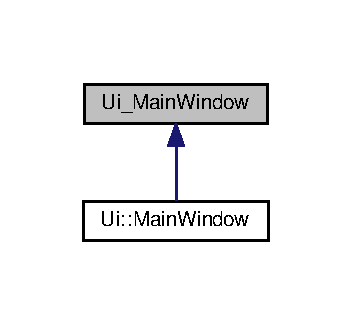
\includegraphics[width=169pt]{class_ui___main_window__inherit__graph}
\end{center}
\end{figure}
\subsection*{Public Member Functions}
\begin{DoxyCompactItemize}
\item 
void {\bfseries setup\+Ui} (Q\+Main\+Window $\ast$\hyperlink{class_main_window}{Main\+Window})\hypertarget{class_ui___main_window_acf4a0872c4c77d8f43a2ec66ed849b58}{}\label{class_ui___main_window_acf4a0872c4c77d8f43a2ec66ed849b58}

\item 
void {\bfseries retranslate\+Ui} (Q\+Main\+Window $\ast$\hyperlink{class_main_window}{Main\+Window})\hypertarget{class_ui___main_window_a097dd160c3534a204904cb374412c618}{}\label{class_ui___main_window_a097dd160c3534a204904cb374412c618}

\end{DoxyCompactItemize}
\subsection*{Public Attributes}
\begin{DoxyCompactItemize}
\item 
Q\+Widget $\ast$ {\bfseries central\+Widget}\hypertarget{class_ui___main_window_a30075506c2116c3ed4ff25e07ae75f81}{}\label{class_ui___main_window_a30075506c2116c3ed4ff25e07ae75f81}

\item 
Q\+Label $\ast$ {\bfseries label\+\_\+larr}\hypertarget{class_ui___main_window_a32587f1e879f5b685d375d2daa20f7a6}{}\label{class_ui___main_window_a32587f1e879f5b685d375d2daa20f7a6}

\item 
Q\+Label $\ast$ {\bfseries label\+\_\+larr2}\hypertarget{class_ui___main_window_a06fc1a01ac3ba3d4d1f75a0e8ab06684}{}\label{class_ui___main_window_a06fc1a01ac3ba3d4d1f75a0e8ab06684}

\item 
Q\+Label $\ast$ {\bfseries label}\hypertarget{class_ui___main_window_ad9c89133780f28e6efa2ec17ceb9cff5}{}\label{class_ui___main_window_ad9c89133780f28e6efa2ec17ceb9cff5}

\item 
Q\+Push\+Button $\ast$ {\bfseries push\+Button\+\_\+ros}\hypertarget{class_ui___main_window_a2667c2b4f9c61bf9895b73d07d4b5172}{}\label{class_ui___main_window_a2667c2b4f9c61bf9895b73d07d4b5172}

\item 
Q\+Push\+Button $\ast$ {\bfseries push\+Button\+\_\+waypoint}\hypertarget{class_ui___main_window_a6b5d7c0f96cdb3276a33746fbcd7e8c7}{}\label{class_ui___main_window_a6b5d7c0f96cdb3276a33746fbcd7e8c7}

\item 
Q\+Push\+Button $\ast$ {\bfseries push\+Button\+\_\+trajectory}\hypertarget{class_ui___main_window_a9d644554288462450d209192c1998095}{}\label{class_ui___main_window_a9d644554288462450d209192c1998095}

\item 
Q\+Push\+Button $\ast$ {\bfseries push\+Button\+\_\+simulation}\hypertarget{class_ui___main_window_afd109ead0ad1ae7ae67ad1df803c9c38}{}\label{class_ui___main_window_afd109ead0ad1ae7ae67ad1df803c9c38}

\item 
Q\+Text\+Edit $\ast$ {\bfseries text\+Edit\+\_\+board}\hypertarget{class_ui___main_window_af13441b9fd874f1aeb2ec5cefaeb0bce}{}\label{class_ui___main_window_af13441b9fd874f1aeb2ec5cefaeb0bce}

\item 
Q\+Push\+Button $\ast$ {\bfseries push\+Button\+\_\+save}\hypertarget{class_ui___main_window_a257d4df0fe652a526e4fddba93c7a7d8}{}\label{class_ui___main_window_a257d4df0fe652a526e4fddba93c7a7d8}

\item 
Q\+Line\+Edit $\ast$ {\bfseries line\+Edit\+\_\+logging\+\_\+dir}\hypertarget{class_ui___main_window_a7ab71242b81ef9d13f83c16f6328f35d}{}\label{class_ui___main_window_a7ab71242b81ef9d13f83c16f6328f35d}

\item 
Q\+Label $\ast$ {\bfseries label\+\_\+2}\hypertarget{class_ui___main_window_a2e2516d755e4dd53fc905dabddf2738a}{}\label{class_ui___main_window_a2e2516d755e4dd53fc905dabddf2738a}

\item 
Q\+Label $\ast$ {\bfseries label\+\_\+3}\hypertarget{class_ui___main_window_a0376fd90247280e7c7957cc70628708c}{}\label{class_ui___main_window_a0376fd90247280e7c7957cc70628708c}

\item 
Q\+Line\+Edit $\ast$ {\bfseries line\+Edit\+\_\+target\+\_\+trajectory}\hypertarget{class_ui___main_window_a4a75bfb754049f89fccef822cad712d6}{}\label{class_ui___main_window_a4a75bfb754049f89fccef822cad712d6}

\item 
Q\+Push\+Button $\ast$ {\bfseries push\+Button\+\_\+load}\hypertarget{class_ui___main_window_a67832089879377ce16b3f26fbb2cc3f2}{}\label{class_ui___main_window_a67832089879377ce16b3f26fbb2cc3f2}

\item 
Q\+Push\+Button $\ast$ {\bfseries push\+Button\+\_\+clear}\hypertarget{class_ui___main_window_a5d7af3b0fdbc605e3fd8ae6ceffa0d29}{}\label{class_ui___main_window_a5d7af3b0fdbc605e3fd8ae6ceffa0d29}

\item 
Q\+Push\+Button $\ast$ {\bfseries push\+Button\+\_\+undo}\hypertarget{class_ui___main_window_ab3fd048b1a1dee328d8e1b433955bf29}{}\label{class_ui___main_window_ab3fd048b1a1dee328d8e1b433955bf29}

\item 
Q\+Label $\ast$ {\bfseries label\+\_\+4}\hypertarget{class_ui___main_window_a78c7e10730b43c6700cd7216911ed76a}{}\label{class_ui___main_window_a78c7e10730b43c6700cd7216911ed76a}

\item 
Q\+Line\+Edit $\ast$ {\bfseries line\+Edit\+\_\+tf}\hypertarget{class_ui___main_window_afc0d94ce5096c619c413cfae9b62014c}{}\label{class_ui___main_window_afc0d94ce5096c619c413cfae9b62014c}

\item 
Q\+Push\+Button $\ast$ {\bfseries push\+Button\+\_\+chaser}\hypertarget{class_ui___main_window_a9e8499b7c9a9717499abde993da72ed5}{}\label{class_ui___main_window_a9e8499b7c9a9717499abde993da72ed5}

\item 
Q\+Menu\+Bar $\ast$ {\bfseries menu\+Bar}\hypertarget{class_ui___main_window_a2be1c24ec9adfca18e1dcc951931457f}{}\label{class_ui___main_window_a2be1c24ec9adfca18e1dcc951931457f}

\item 
Q\+Menu $\ast$ {\bfseries menu\+Auto\+\_\+chaser}\hypertarget{class_ui___main_window_a8946bc17fa5b33e1c89ef82fdacab1d8}{}\label{class_ui___main_window_a8946bc17fa5b33e1c89ef82fdacab1d8}

\item 
Q\+Tool\+Bar $\ast$ {\bfseries main\+Tool\+Bar}\hypertarget{class_ui___main_window_a5172877001c8c7b4e0f6de50421867d1}{}\label{class_ui___main_window_a5172877001c8c7b4e0f6de50421867d1}

\item 
Q\+Status\+Bar $\ast$ {\bfseries status\+Bar}\hypertarget{class_ui___main_window_a50fa481337604bcc8bf68de18ab16ecd}{}\label{class_ui___main_window_a50fa481337604bcc8bf68de18ab16ecd}

\end{DoxyCompactItemize}


The documentation for this class was generated from the following file\+:\begin{DoxyCompactItemize}
\item 
src/build-\/qt\+\_\+ui-\/\+Desktop-\/\+Debug/ui\+\_\+mainwindow.\+h\end{DoxyCompactItemize}

\hypertarget{class_wrapper}{}\section{Wrapper Class Reference}
\label{class_wrapper}\index{Wrapper@{Wrapper}}


{\ttfamily \#include $<$Wrapper.\+h$>$}



Collaboration diagram for Wrapper\+:
\nopagebreak
\begin{figure}[H]
\begin{center}
\leavevmode
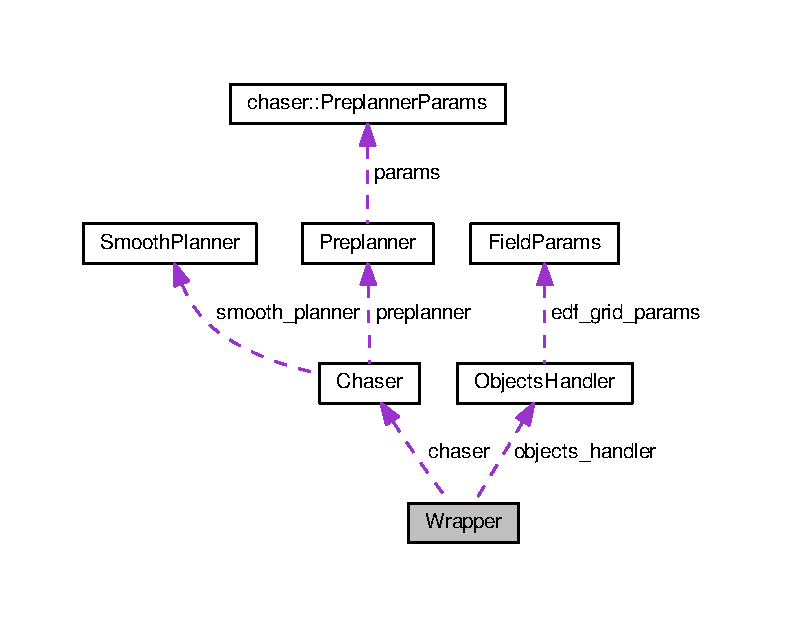
\includegraphics[width=243pt]{class_wrapper__coll__graph}
\end{center}
\end{figure}
\subsection*{Public Member Functions}
\begin{DoxyCompactItemize}
\item 
\hyperlink{class_wrapper_aa40ce9fcba8ab60bf01bcb0913144b4a}{Wrapper} ()
\item 
void \hyperlink{class_wrapper_af336781e7d75d525e7b152366a0e0d93}{init} (ros\+::\+Node\+Handle nh)
\item 
void \hyperlink{class_wrapper_a009ee5c325926f92df42319d5469a376}{session} (double t)
\item 
bool \hyperlink{class_wrapper_a21a0e115ea80e053e4f2defd1362b92f}{trigger\+\_\+chasing} (Time\+Series chasing\+\_\+knots)
\item 
bool \hyperlink{class_wrapper_a2da6448c77dd4edb054de4130b1fc883}{trigger\+\_\+chasing} (vector$<$ Point $>$ target\+\_\+seq, Time\+Series chasing\+\_\+knots)
\item 
geometry\+\_\+msgs\+::\+Pose\+Stamped \hyperlink{class_wrapper_ac2338df9e7b31f3291ed1cbd137a6f14}{get\+\_\+control\+\_\+pose} (double t\+\_\+eval)
\begin{DoxyCompactList}\small\item\em evalate the latest control pose from chaser \end{DoxyCompactList}\item 
void \hyperlink{class_wrapper_a94a786272ea8120469cb476d021c5b76}{pub\+\_\+control\+\_\+pose} (double t\+\_\+eval)
\begin{DoxyCompactList}\small\item\em publish the control visualization (geometry\+\_\+msgs) \end{DoxyCompactList}\item 
void \hyperlink{class_wrapper_a7f0e09c8a675991a3c987e41c6b9ff9d}{pub\+\_\+control\+\_\+traj} (double t\+\_\+eval)
\begin{DoxyCompactList}\small\item\em publish the control visualization (trajectory\+\_\+msgs) \end{DoxyCompactList}\item 
void \hyperlink{class_wrapper_a3fcc1a8192f2e72f501f2e9912a0ef41}{pub\+\_\+control\+\_\+pose} (Pose\+Stamped control\+\_\+pose)
\item 
void \hyperlink{class_wrapper_a754999f67924fbda6dc3b3e38377af79}{pub\+\_\+control\+\_\+traj} (Pose\+Stamped control\+\_\+pose)
\end{DoxyCompactItemize}
\subsection*{Public Attributes}
\begin{DoxyCompactItemize}
\item 
int \hyperlink{class_wrapper_a4b4e8407edf38f99eb9d5a0cd4a0116b}{run\+\_\+mode}
\item 
\hyperlink{class_objects_handler}{Objects\+Handler} \hyperlink{class_wrapper_a8cddd5ffbaeb5ab0b5d8d8d0c74f810f}{objects\+\_\+handler}
\item 
\hyperlink{class_chaser}{Chaser} \hyperlink{class_wrapper_a750309ad3470e20a80e9d72b0d7e34cb}{chaser}
\end{DoxyCompactItemize}


\subsection{Detailed Description}


Definition at line 6 of file Wrapper.\+h.



\subsection{Constructor \& Destructor Documentation}
\index{Wrapper@{Wrapper}!Wrapper@{Wrapper}}
\index{Wrapper@{Wrapper}!Wrapper@{Wrapper}}
\subsubsection[{\texorpdfstring{Wrapper()}{Wrapper()}}]{\setlength{\rightskip}{0pt plus 5cm}Wrapper\+::\+Wrapper (
\begin{DoxyParamCaption}
{}
\end{DoxyParamCaption}
)}\hypertarget{class_wrapper_aa40ce9fcba8ab60bf01bcb0913144b4a}{}\label{class_wrapper_aa40ce9fcba8ab60bf01bcb0913144b4a}


Definition at line 3 of file Wrapper.\+cpp.



\subsection{Member Function Documentation}
\index{Wrapper@{Wrapper}!get\+\_\+control\+\_\+pose@{get\+\_\+control\+\_\+pose}}
\index{get\+\_\+control\+\_\+pose@{get\+\_\+control\+\_\+pose}!Wrapper@{Wrapper}}
\subsubsection[{\texorpdfstring{get\+\_\+control\+\_\+pose(double t\+\_\+eval)}{get_control_pose(double t_eval)}}]{\setlength{\rightskip}{0pt plus 5cm}geometry\+\_\+msgs\+::\+Pose\+Stamped Wrapper\+::get\+\_\+control\+\_\+pose (
\begin{DoxyParamCaption}
\item[{double}]{t\+\_\+eval}
\end{DoxyParamCaption}
)}\hypertarget{class_wrapper_ac2338df9e7b31f3291ed1cbd137a6f14}{}\label{class_wrapper_ac2338df9e7b31f3291ed1cbd137a6f14}


evalate the latest control pose from chaser 


\begin{DoxyParams}{Parameters}
{\em t\+\_\+eval} & the evaluation time \\
\hline
\end{DoxyParams}
\begin{DoxyReturn}{Returns}
geometry\+\_\+msgs\+::\+Pose\+Stamped the control pose for M\+AV 
\end{DoxyReturn}


Definition at line 131 of file Wrapper.\+cpp.



Here is the call graph for this function\+:
\nopagebreak
\begin{figure}[H]
\begin{center}
\leavevmode
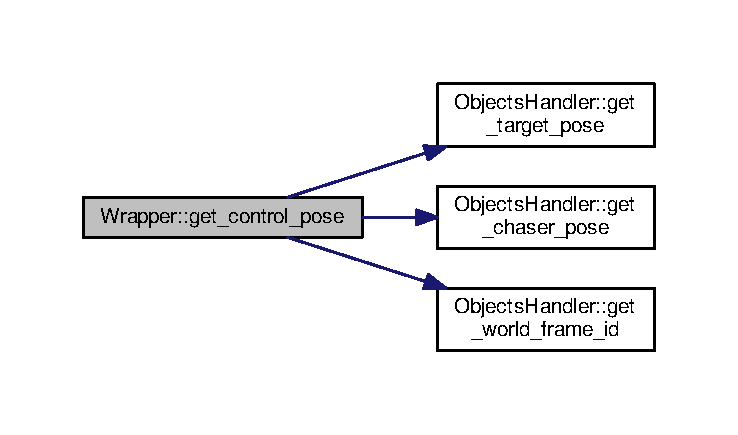
\includegraphics[width=350pt]{class_wrapper_ac2338df9e7b31f3291ed1cbd137a6f14_cgraph}
\end{center}
\end{figure}




Here is the caller graph for this function\+:
\nopagebreak
\begin{figure}[H]
\begin{center}
\leavevmode
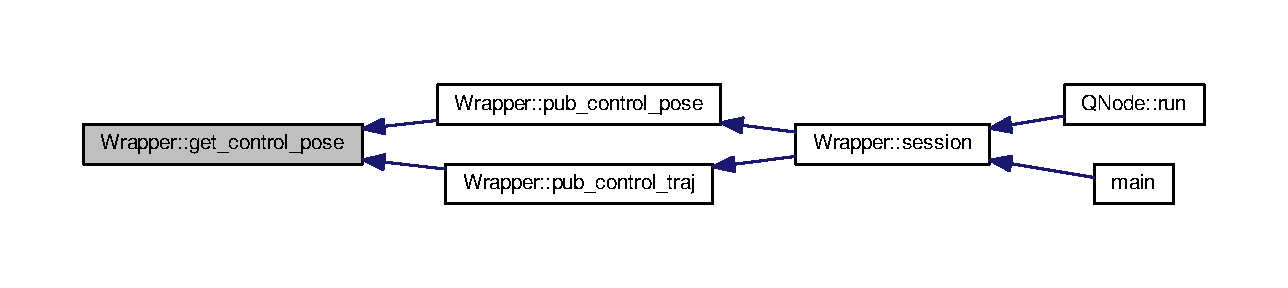
\includegraphics[width=350pt]{class_wrapper_ac2338df9e7b31f3291ed1cbd137a6f14_icgraph}
\end{center}
\end{figure}


\index{Wrapper@{Wrapper}!init@{init}}
\index{init@{init}!Wrapper@{Wrapper}}
\subsubsection[{\texorpdfstring{init(ros\+::\+Node\+Handle nh)}{init(ros::NodeHandle nh)}}]{\setlength{\rightskip}{0pt plus 5cm}void Wrapper\+::init (
\begin{DoxyParamCaption}
\item[{ros\+::\+Node\+Handle}]{nh}
\end{DoxyParamCaption}
)}\hypertarget{class_wrapper_af336781e7d75d525e7b152366a0e0d93}{}\label{class_wrapper_af336781e7d75d525e7b152366a0e0d93}


Definition at line 5 of file Wrapper.\+cpp.



Here is the call graph for this function\+:
\nopagebreak
\begin{figure}[H]
\begin{center}
\leavevmode
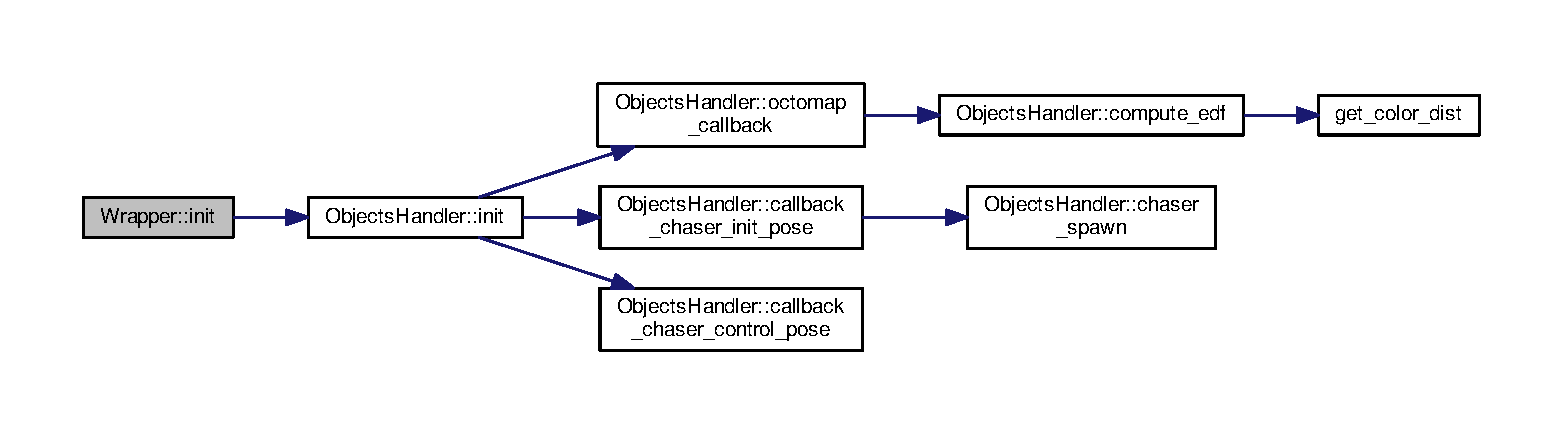
\includegraphics[width=350pt]{class_wrapper_af336781e7d75d525e7b152366a0e0d93_cgraph}
\end{center}
\end{figure}




Here is the caller graph for this function\+:
\nopagebreak
\begin{figure}[H]
\begin{center}
\leavevmode
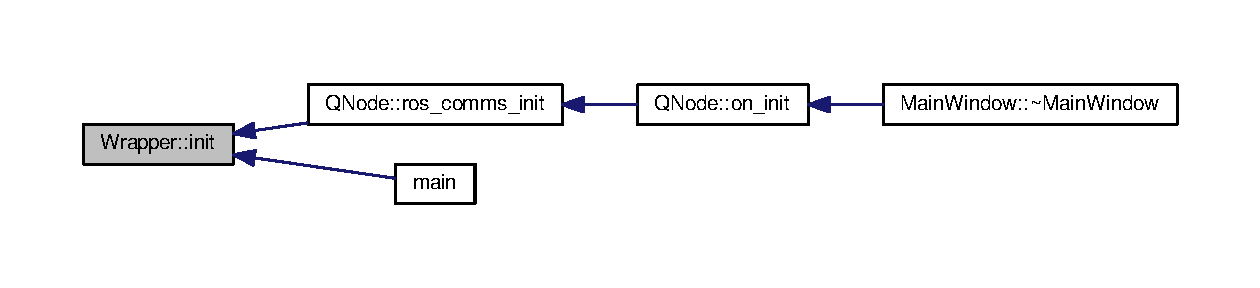
\includegraphics[width=350pt]{class_wrapper_af336781e7d75d525e7b152366a0e0d93_icgraph}
\end{center}
\end{figure}


\index{Wrapper@{Wrapper}!pub\+\_\+control\+\_\+pose@{pub\+\_\+control\+\_\+pose}}
\index{pub\+\_\+control\+\_\+pose@{pub\+\_\+control\+\_\+pose}!Wrapper@{Wrapper}}
\subsubsection[{\texorpdfstring{pub\+\_\+control\+\_\+pose(double t\+\_\+eval)}{pub_control_pose(double t_eval)}}]{\setlength{\rightskip}{0pt plus 5cm}void Wrapper\+::pub\+\_\+control\+\_\+pose (
\begin{DoxyParamCaption}
\item[{double}]{t\+\_\+eval}
\end{DoxyParamCaption}
)}\hypertarget{class_wrapper_a94a786272ea8120469cb476d021c5b76}{}\label{class_wrapper_a94a786272ea8120469cb476d021c5b76}


publish the control visualization (geometry\+\_\+msgs) 


\begin{DoxyParams}{Parameters}
{\em t\+\_\+eval} & evaluation time \\
\hline
\end{DoxyParams}


Definition at line 222 of file Wrapper.\+cpp.



Here is the call graph for this function\+:
\nopagebreak
\begin{figure}[H]
\begin{center}
\leavevmode
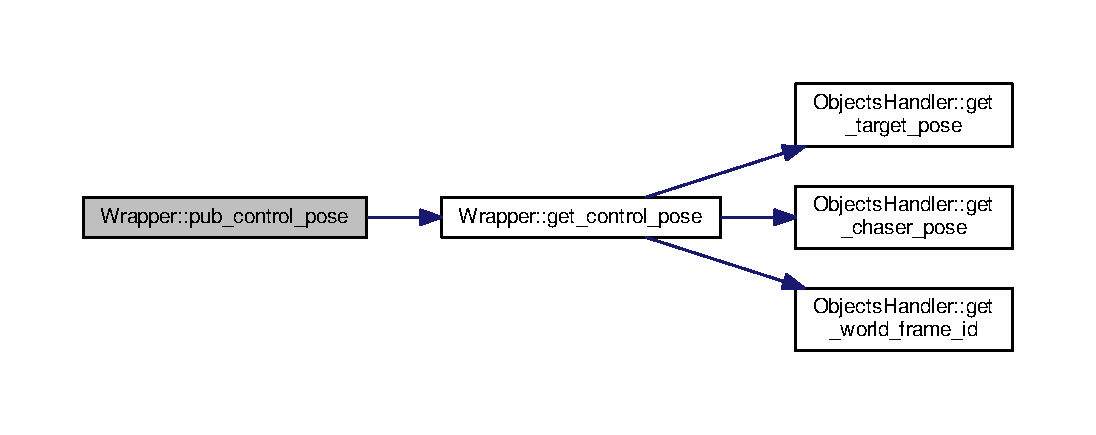
\includegraphics[width=350pt]{class_wrapper_a94a786272ea8120469cb476d021c5b76_cgraph}
\end{center}
\end{figure}




Here is the caller graph for this function\+:
\nopagebreak
\begin{figure}[H]
\begin{center}
\leavevmode
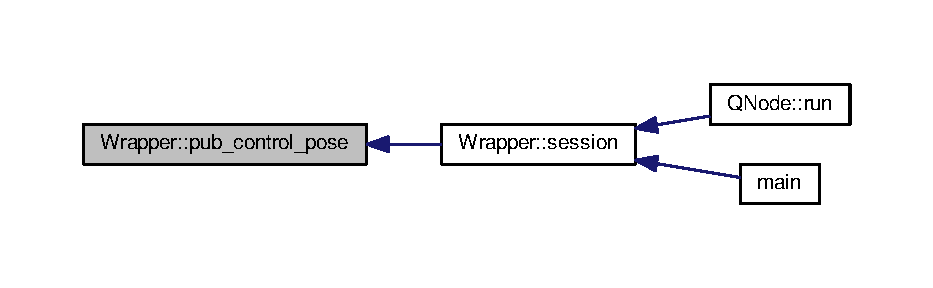
\includegraphics[width=350pt]{class_wrapper_a94a786272ea8120469cb476d021c5b76_icgraph}
\end{center}
\end{figure}


\index{Wrapper@{Wrapper}!pub\+\_\+control\+\_\+pose@{pub\+\_\+control\+\_\+pose}}
\index{pub\+\_\+control\+\_\+pose@{pub\+\_\+control\+\_\+pose}!Wrapper@{Wrapper}}
\subsubsection[{\texorpdfstring{pub\+\_\+control\+\_\+pose(\+Pose\+Stamped control\+\_\+pose)}{pub_control_pose(PoseStamped control_pose)}}]{\setlength{\rightskip}{0pt plus 5cm}void Wrapper\+::pub\+\_\+control\+\_\+pose (
\begin{DoxyParamCaption}
\item[{Pose\+Stamped}]{control\+\_\+pose}
\end{DoxyParamCaption}
)}\hypertarget{class_wrapper_a3fcc1a8192f2e72f501f2e9912a0ef41}{}\label{class_wrapper_a3fcc1a8192f2e72f501f2e9912a0ef41}
\index{Wrapper@{Wrapper}!pub\+\_\+control\+\_\+traj@{pub\+\_\+control\+\_\+traj}}
\index{pub\+\_\+control\+\_\+traj@{pub\+\_\+control\+\_\+traj}!Wrapper@{Wrapper}}
\subsubsection[{\texorpdfstring{pub\+\_\+control\+\_\+traj(double t\+\_\+eval)}{pub_control_traj(double t_eval)}}]{\setlength{\rightskip}{0pt plus 5cm}void Wrapper\+::pub\+\_\+control\+\_\+traj (
\begin{DoxyParamCaption}
\item[{double}]{t\+\_\+eval}
\end{DoxyParamCaption}
)}\hypertarget{class_wrapper_a7f0e09c8a675991a3c987e41c6b9ff9d}{}\label{class_wrapper_a7f0e09c8a675991a3c987e41c6b9ff9d}


publish the control visualization (trajectory\+\_\+msgs) 


\begin{DoxyParams}{Parameters}
{\em t\+\_\+eval} & \\
\hline
\end{DoxyParams}


Definition at line 235 of file Wrapper.\+cpp.



Here is the call graph for this function\+:
\nopagebreak
\begin{figure}[H]
\begin{center}
\leavevmode
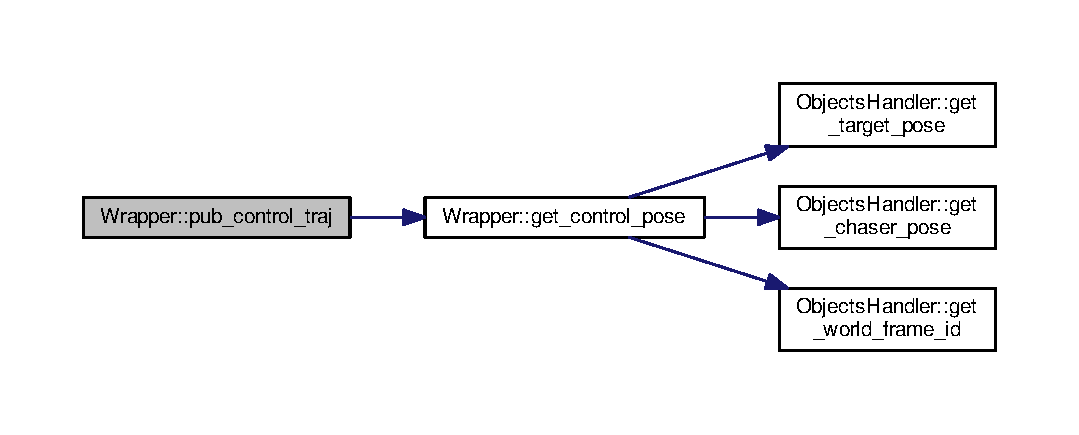
\includegraphics[width=350pt]{class_wrapper_a7f0e09c8a675991a3c987e41c6b9ff9d_cgraph}
\end{center}
\end{figure}




Here is the caller graph for this function\+:
\nopagebreak
\begin{figure}[H]
\begin{center}
\leavevmode
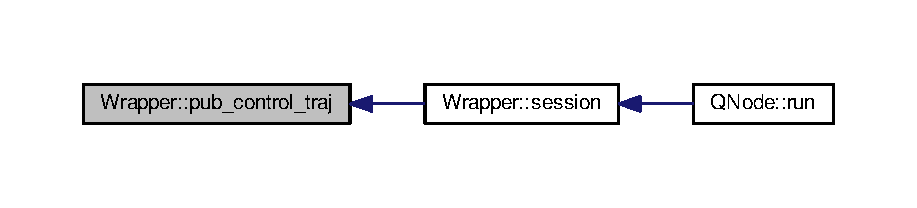
\includegraphics[width=350pt]{class_wrapper_a7f0e09c8a675991a3c987e41c6b9ff9d_icgraph}
\end{center}
\end{figure}


\index{Wrapper@{Wrapper}!pub\+\_\+control\+\_\+traj@{pub\+\_\+control\+\_\+traj}}
\index{pub\+\_\+control\+\_\+traj@{pub\+\_\+control\+\_\+traj}!Wrapper@{Wrapper}}
\subsubsection[{\texorpdfstring{pub\+\_\+control\+\_\+traj(\+Pose\+Stamped control\+\_\+pose)}{pub_control_traj(PoseStamped control_pose)}}]{\setlength{\rightskip}{0pt plus 5cm}void Wrapper\+::pub\+\_\+control\+\_\+traj (
\begin{DoxyParamCaption}
\item[{Pose\+Stamped}]{control\+\_\+pose}
\end{DoxyParamCaption}
)}\hypertarget{class_wrapper_a754999f67924fbda6dc3b3e38377af79}{}\label{class_wrapper_a754999f67924fbda6dc3b3e38377af79}
\index{Wrapper@{Wrapper}!session@{session}}
\index{session@{session}!Wrapper@{Wrapper}}
\subsubsection[{\texorpdfstring{session(double t)}{session(double t)}}]{\setlength{\rightskip}{0pt plus 5cm}void Wrapper\+::session (
\begin{DoxyParamCaption}
\item[{double}]{t}
\end{DoxyParamCaption}
)}\hypertarget{class_wrapper_a009ee5c325926f92df42319d5469a376}{}\label{class_wrapper_a009ee5c325926f92df42319d5469a376}


Definition at line 28 of file Wrapper.\+cpp.



Here is the call graph for this function\+:
\nopagebreak
\begin{figure}[H]
\begin{center}
\leavevmode
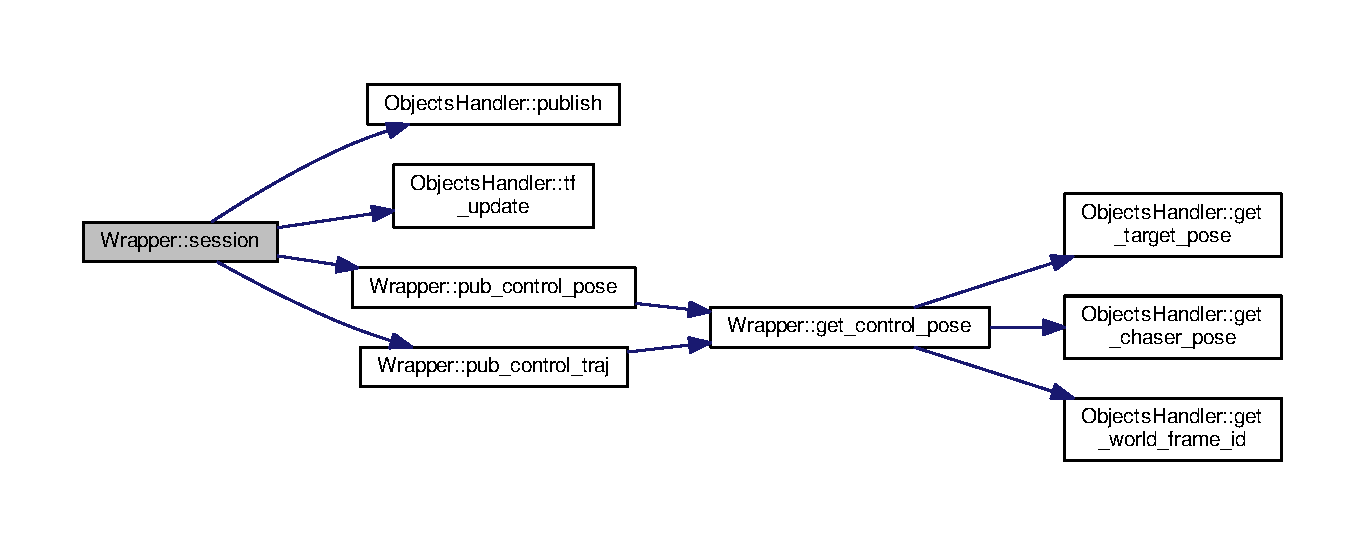
\includegraphics[width=350pt]{class_wrapper_a009ee5c325926f92df42319d5469a376_cgraph}
\end{center}
\end{figure}




Here is the caller graph for this function\+:
\nopagebreak
\begin{figure}[H]
\begin{center}
\leavevmode
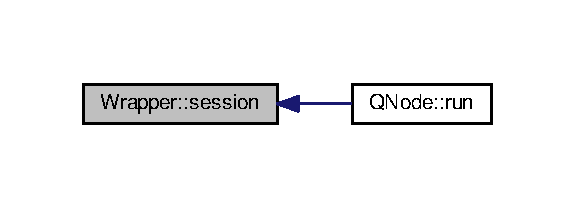
\includegraphics[width=276pt]{class_wrapper_a009ee5c325926f92df42319d5469a376_icgraph}
\end{center}
\end{figure}


\index{Wrapper@{Wrapper}!trigger\+\_\+chasing@{trigger\+\_\+chasing}}
\index{trigger\+\_\+chasing@{trigger\+\_\+chasing}!Wrapper@{Wrapper}}
\subsubsection[{\texorpdfstring{trigger\+\_\+chasing(\+Time\+Series chasing\+\_\+knots)}{trigger_chasing(TimeSeries chasing_knots)}}]{\setlength{\rightskip}{0pt plus 5cm}bool Wrapper\+::trigger\+\_\+chasing (
\begin{DoxyParamCaption}
\item[{Time\+Series}]{chasing\+\_\+knots}
\end{DoxyParamCaption}
)}\hypertarget{class_wrapper_a21a0e115ea80e053e4f2defd1362b92f}{}\label{class_wrapper_a21a0e115ea80e053e4f2defd1362b92f}


Definition at line 59 of file Wrapper.\+cpp.



Here is the call graph for this function\+:
\nopagebreak
\begin{figure}[H]
\begin{center}
\leavevmode
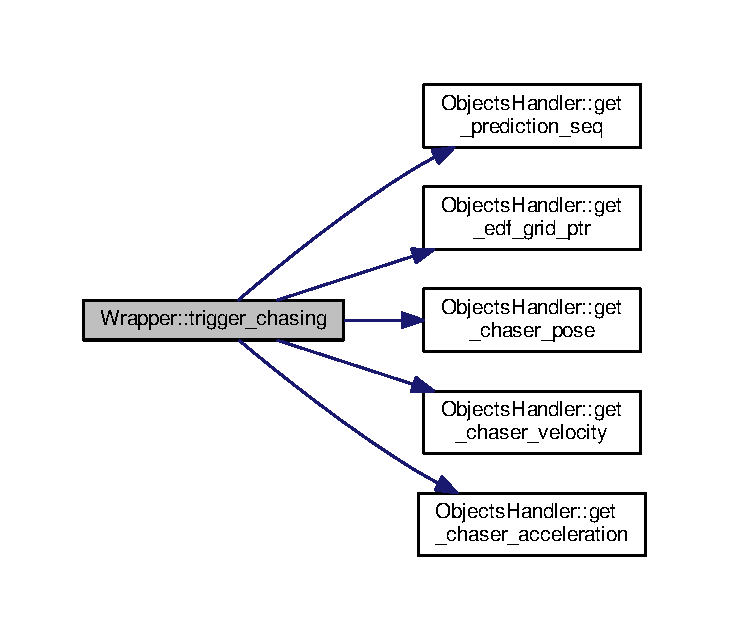
\includegraphics[width=350pt]{class_wrapper_a21a0e115ea80e053e4f2defd1362b92f_cgraph}
\end{center}
\end{figure}




Here is the caller graph for this function\+:
\nopagebreak
\begin{figure}[H]
\begin{center}
\leavevmode
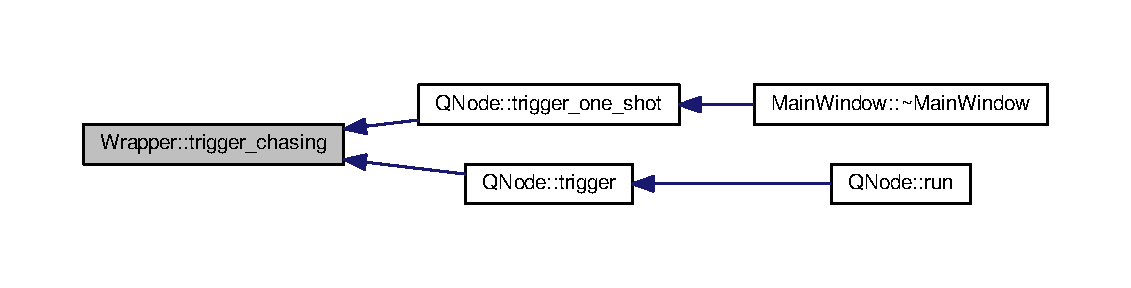
\includegraphics[width=350pt]{class_wrapper_a21a0e115ea80e053e4f2defd1362b92f_icgraph}
\end{center}
\end{figure}


\index{Wrapper@{Wrapper}!trigger\+\_\+chasing@{trigger\+\_\+chasing}}
\index{trigger\+\_\+chasing@{trigger\+\_\+chasing}!Wrapper@{Wrapper}}
\subsubsection[{\texorpdfstring{trigger\+\_\+chasing(vector$<$ Point $>$ target\+\_\+seq, Time\+Series chasing\+\_\+knots)}{trigger_chasing(vector< Point > target_seq, TimeSeries chasing_knots)}}]{\setlength{\rightskip}{0pt plus 5cm}bool Wrapper\+::trigger\+\_\+chasing (
\begin{DoxyParamCaption}
\item[{vector$<$ Point $>$}]{target\+\_\+seq, }
\item[{Time\+Series}]{chasing\+\_\+knots}
\end{DoxyParamCaption}
)}\hypertarget{class_wrapper_a2da6448c77dd4edb054de4130b1fc883}{}\label{class_wrapper_a2da6448c77dd4edb054de4130b1fc883}


Definition at line 92 of file Wrapper.\+cpp.



Here is the call graph for this function\+:
\nopagebreak
\begin{figure}[H]
\begin{center}
\leavevmode
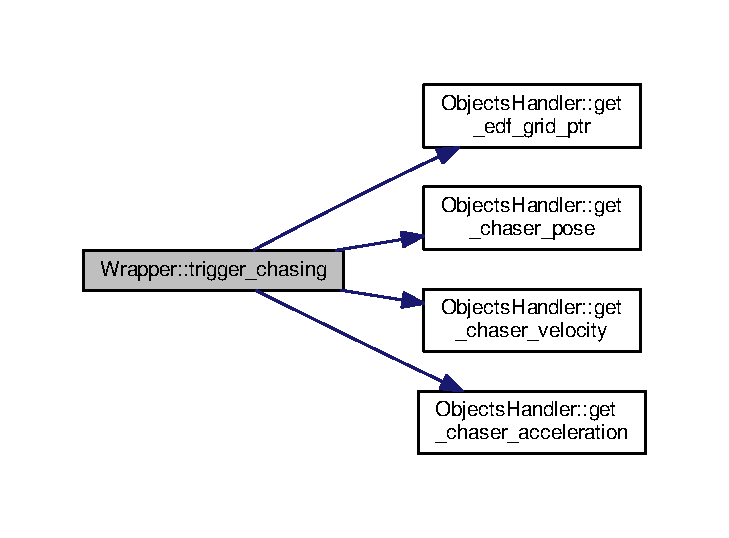
\includegraphics[width=350pt]{class_wrapper_a2da6448c77dd4edb054de4130b1fc883_cgraph}
\end{center}
\end{figure}




\subsection{Member Data Documentation}
\index{Wrapper@{Wrapper}!chaser@{chaser}}
\index{chaser@{chaser}!Wrapper@{Wrapper}}
\subsubsection[{\texorpdfstring{chaser}{chaser}}]{\setlength{\rightskip}{0pt plus 5cm}{\bf Chaser} Wrapper\+::chaser}\hypertarget{class_wrapper_a750309ad3470e20a80e9d72b0d7e34cb}{}\label{class_wrapper_a750309ad3470e20a80e9d72b0d7e34cb}


Definition at line 31 of file Wrapper.\+h.

\index{Wrapper@{Wrapper}!objects\+\_\+handler@{objects\+\_\+handler}}
\index{objects\+\_\+handler@{objects\+\_\+handler}!Wrapper@{Wrapper}}
\subsubsection[{\texorpdfstring{objects\+\_\+handler}{objects_handler}}]{\setlength{\rightskip}{0pt plus 5cm}{\bf Objects\+Handler} Wrapper\+::objects\+\_\+handler}\hypertarget{class_wrapper_a8cddd5ffbaeb5ab0b5d8d8d0c74f810f}{}\label{class_wrapper_a8cddd5ffbaeb5ab0b5d8d8d0c74f810f}


Definition at line 30 of file Wrapper.\+h.

\index{Wrapper@{Wrapper}!run\+\_\+mode@{run\+\_\+mode}}
\index{run\+\_\+mode@{run\+\_\+mode}!Wrapper@{Wrapper}}
\subsubsection[{\texorpdfstring{run\+\_\+mode}{run_mode}}]{\setlength{\rightskip}{0pt plus 5cm}int Wrapper\+::run\+\_\+mode}\hypertarget{class_wrapper_a4b4e8407edf38f99eb9d5a0cd4a0116b}{}\label{class_wrapper_a4b4e8407edf38f99eb9d5a0cd4a0116b}


Definition at line 29 of file Wrapper.\+h.



The documentation for this class was generated from the following files\+:\begin{DoxyCompactItemize}
\item 
include/auto\+\_\+chaser/\hyperlink{_wrapper_8h}{Wrapper.\+h}\item 
src/auto\+\_\+chaser/\hyperlink{_wrapper_8cpp}{Wrapper.\+cpp}\end{DoxyCompactItemize}

\chapter{File Documentation}
\hypertarget{generate__cached__setup_8py}{}\section{build/catkin\+\_\+generated/generate\+\_\+cached\+\_\+setup.py File Reference}
\label{generate__cached__setup_8py}\index{build/catkin\+\_\+generated/generate\+\_\+cached\+\_\+setup.\+py@{build/catkin\+\_\+generated/generate\+\_\+cached\+\_\+setup.\+py}}
\subsection*{Namespaces}
\begin{DoxyCompactItemize}
\item 
 \hyperlink{namespacegenerate__cached__setup}{generate\+\_\+cached\+\_\+setup}
\end{DoxyCompactItemize}
\subsection*{Variables}
\begin{DoxyCompactItemize}
\item 
\hyperlink{namespacegenerate__cached__setup_a72579fd01529a79bab20d99291889d3f}{generate\+\_\+cached\+\_\+setup.\+python\+\_\+path} = os.\+path.\+join(workspace, \textquotesingle{}lib/python2.\+7/dist-\/packages\textquotesingle{})
\item 
\hyperlink{namespacegenerate__cached__setup_a52601295006f2366a311c4453d8f2f2e}{generate\+\_\+cached\+\_\+setup.\+code} = generate\+\_\+environment\+\_\+script(\textquotesingle{}/home/jbs/catkin\+\_\+ws/src/auto\+\_\+chaser/build/devel/env.\+sh\textquotesingle{})
\item 
string \hyperlink{namespacegenerate__cached__setup_a0265aee5075ee1eb701ff69c98ad6793}{generate\+\_\+cached\+\_\+setup.\+output\+\_\+filename} = \textquotesingle{}/home/jbs/catkin\+\_\+ws/src/auto\+\_\+chaser/build/catkin\+\_\+generated/setup\+\_\+cached.\+sh\textquotesingle{}
\item 
\hyperlink{namespacegenerate__cached__setup_a10081e5abedae9bd46dd91202096e789}{generate\+\_\+cached\+\_\+setup.\+mode} = os.\+stat(output\+\_\+filename).st\+\_\+mode
\end{DoxyCompactItemize}

\hypertarget{catkin__generated_2installspace_2__setup__util_8py}{}\section{build/catkin\+\_\+generated/installspace/\+\_\+setup\+\_\+util.py File Reference}
\label{catkin__generated_2installspace_2__setup__util_8py}\index{build/catkin\+\_\+generated/installspace/\+\_\+setup\+\_\+util.\+py@{build/catkin\+\_\+generated/installspace/\+\_\+setup\+\_\+util.\+py}}
\subsection*{Namespaces}
\begin{DoxyCompactItemize}
\item 
 \hyperlink{namespace__setup__util}{\+\_\+setup\+\_\+util}
\end{DoxyCompactItemize}
\subsection*{Functions}
\begin{DoxyCompactItemize}
\item 
def \hyperlink{namespace__setup__util_af3030db6102b5aa35cd354a2fb6cca03}{\+\_\+setup\+\_\+util.\+rollback\+\_\+env\+\_\+variables} (environ, env\+\_\+var\+\_\+subfolders)
\item 
def \hyperlink{namespace__setup__util_af05661e87b3270e8bfd0fbc18a5eeec4}{\+\_\+setup\+\_\+util.\+\_\+rollback\+\_\+env\+\_\+variable} (environ, name, subfolders)
\item 
def \hyperlink{namespace__setup__util_ab2be07aa31918f1e1e34d6b7c4d66fcb}{\+\_\+setup\+\_\+util.\+\_\+get\+\_\+workspaces} (environ, include\+\_\+fuerte=False, include\+\_\+non\+\_\+existing=False)
\item 
def \hyperlink{namespace__setup__util_a832417d18b85bd1d276a87547e86f860}{\+\_\+setup\+\_\+util.\+prepend\+\_\+env\+\_\+variables} (environ, env\+\_\+var\+\_\+subfolders, workspaces)
\item 
def \hyperlink{namespace__setup__util_a74a1f8575ed82282d03f7795c9ba6e45}{\+\_\+setup\+\_\+util.\+\_\+prefix\+\_\+env\+\_\+variable} (environ, name, paths, subfolders)
\item 
def \hyperlink{namespace__setup__util_ad56c24837fa4eddc63c03fbc7035628f}{\+\_\+setup\+\_\+util.\+assignment} (key, value)
\item 
def \hyperlink{namespace__setup__util_abe8c95c4cfe8b1374dacd5f91d984353}{\+\_\+setup\+\_\+util.\+comment} (msg)
\item 
def \hyperlink{namespace__setup__util_ae78d86b2c4279f5b8b1acaa146c35802}{\+\_\+setup\+\_\+util.\+prepend} (environ, key, prefix)
\item 
def \hyperlink{namespace__setup__util_a73de35ca77f260af6691470342ab49ce}{\+\_\+setup\+\_\+util.\+find\+\_\+env\+\_\+hooks} (environ, cmake\+\_\+prefix\+\_\+path)
\item 
def \hyperlink{namespace__setup__util_a57d9ecb280810c9a5409d44aeb9d0a25}{\+\_\+setup\+\_\+util.\+\_\+parse\+\_\+arguments} (args=None)
\end{DoxyCompactItemize}
\subsection*{Variables}
\begin{DoxyCompactItemize}
\item 
string \hyperlink{namespace__setup__util_a3fa0ca5a460a71a43cbc3d4954ab1f10}{\+\_\+setup\+\_\+util.\+C\+A\+T\+K\+I\+N\+\_\+\+M\+A\+R\+K\+E\+R\+\_\+\+F\+I\+LE} = \textquotesingle{}.catkin\textquotesingle{}
\item 
\hyperlink{namespace__setup__util_ae9fca6a80a6923f4580be72f68fee325}{\+\_\+setup\+\_\+util.\+system} = platform.\+system()
\item 
tuple \hyperlink{namespace__setup__util_aecbb100ce6f94bb3c7e16d58fde05f96}{\+\_\+setup\+\_\+util.\+I\+S\+\_\+\+D\+A\+R\+W\+IN} = (system == \textquotesingle{}Darwin\textquotesingle{})
\item 
tuple \hyperlink{namespace__setup__util_a6fe69c2dbd92959b6651a28cbb846e6e}{\+\_\+setup\+\_\+util.\+I\+S\+\_\+\+W\+I\+N\+D\+O\+WS} = (system == \textquotesingle{}Windows\textquotesingle{})
\item 
dictionary \hyperlink{namespace__setup__util_aa31804f1be8660156ce9394b33c68dc4}{\+\_\+setup\+\_\+util.\+E\+N\+V\+\_\+\+V\+A\+R\+\_\+\+S\+U\+B\+F\+O\+L\+D\+E\+RS}
\item 
\hyperlink{namespace__setup__util_a547963d07c6371df1c51b1384a2dec28}{\+\_\+setup\+\_\+util.\+args} = \+\_\+parse\+\_\+arguments()
\item 
\hyperlink{namespace__setup__util_acdce690b925de33d6249bbbfa1109d61}{\+\_\+setup\+\_\+util.\+e}
\item 
\hyperlink{namespace__setup__util_aea63a1b32cc79bc3d872ab7cb30dd07e}{\+\_\+setup\+\_\+util.\+file}
\item 
string \hyperlink{namespace__setup__util_a57afd3d2c076955fb715f3e72ef098eb}{\+\_\+setup\+\_\+util.\+C\+M\+A\+K\+E\+\_\+\+P\+R\+E\+F\+I\+X\+\_\+\+P\+A\+TH} = \textquotesingle{}/home/jbs/catkin\+\_\+ws/devel;/opt/ros/kinetic\textquotesingle{}
\item 
\hyperlink{namespace__setup__util_a83d25140acd7788bbcb95843fe38e639}{\+\_\+setup\+\_\+util.\+base\+\_\+path} = os.\+path.\+dirname(\+\_\+\+\_\+file\+\_\+\+\_\+)
\item 
\hyperlink{namespace__setup__util_a9a935bdd9ee1aa0327161025bb18c136}{\+\_\+setup\+\_\+util.\+environ} = dict(os.\+environ)
\item 
list \hyperlink{namespace__setup__util_a8618d8be5f729d4c9696daa5e083a001}{\+\_\+setup\+\_\+util.\+lines} = \mbox{[}$\,$\mbox{]}
\end{DoxyCompactItemize}

\hypertarget{devel_2__setup__util_8py}{}\section{build/devel/\+\_\+setup\+\_\+util.py File Reference}
\label{devel_2__setup__util_8py}\index{build/devel/\+\_\+setup\+\_\+util.\+py@{build/devel/\+\_\+setup\+\_\+util.\+py}}
\subsection*{Namespaces}
\begin{DoxyCompactItemize}
\item 
 \hyperlink{namespace__setup__util}{\+\_\+setup\+\_\+util}
\end{DoxyCompactItemize}
\subsection*{Functions}
\begin{DoxyCompactItemize}
\item 
def \hyperlink{namespace__setup__util_af3030db6102b5aa35cd354a2fb6cca03}{\+\_\+setup\+\_\+util.\+rollback\+\_\+env\+\_\+variables} (environ, env\+\_\+var\+\_\+subfolders)
\item 
def \hyperlink{namespace__setup__util_a832417d18b85bd1d276a87547e86f860}{\+\_\+setup\+\_\+util.\+prepend\+\_\+env\+\_\+variables} (environ, env\+\_\+var\+\_\+subfolders, workspaces)
\item 
def \hyperlink{namespace__setup__util_ad56c24837fa4eddc63c03fbc7035628f}{\+\_\+setup\+\_\+util.\+assignment} (key, value)
\item 
def \hyperlink{namespace__setup__util_abe8c95c4cfe8b1374dacd5f91d984353}{\+\_\+setup\+\_\+util.\+comment} (msg)
\item 
def \hyperlink{namespace__setup__util_ae78d86b2c4279f5b8b1acaa146c35802}{\+\_\+setup\+\_\+util.\+prepend} (environ, key, prefix)
\item 
def \hyperlink{namespace__setup__util_a73de35ca77f260af6691470342ab49ce}{\+\_\+setup\+\_\+util.\+find\+\_\+env\+\_\+hooks} (environ, cmake\+\_\+prefix\+\_\+path)
\end{DoxyCompactItemize}

\hypertarget{pkg_8develspace_8context_8pc_8py}{}\section{/home/jbs/catkin\+\_\+ws/src/traj\+\_\+gen\+\_\+vis\+\_\+developing/build/catkin\+\_\+generated/pkg.develspace.\+context.\+pc.\+py File Reference}
\label{pkg_8develspace_8context_8pc_8py}\index{/home/jbs/catkin\+\_\+ws/src/traj\+\_\+gen\+\_\+vis\+\_\+developing/build/catkin\+\_\+generated/pkg.\+develspace.\+context.\+pc.\+py@{/home/jbs/catkin\+\_\+ws/src/traj\+\_\+gen\+\_\+vis\+\_\+developing/build/catkin\+\_\+generated/pkg.\+develspace.\+context.\+pc.\+py}}
\subsection*{Namespaces}
\begin{DoxyCompactItemize}
\item 
 \hyperlink{namespacepkg}{pkg}
\end{DoxyCompactItemize}
\subsection*{Variables}
\begin{DoxyCompactItemize}
\item 
string \hyperlink{namespacepkg_ae26c7a5a06b7d738f4d210ca449e6bee}{pkg.\+C\+A\+T\+K\+I\+N\+\_\+\+P\+A\+C\+K\+A\+G\+E\+\_\+\+P\+R\+E\+F\+IX} = \char`\"{}\char`\"{}
\item 
string \hyperlink{namespacepkg_a2760bf8266ff58da440f65ee91b203ab}{pkg.\+P\+R\+O\+J\+E\+C\+T\+\_\+\+P\+K\+G\+\_\+\+C\+O\+N\+F\+I\+G\+\_\+\+I\+N\+C\+L\+U\+D\+E\+\_\+\+D\+I\+RS} = \char`\"{}/home/jbs/catkin\+\_\+ws/src/auto\+\_\+chaser/include\char`\"{}
\item 
string \hyperlink{namespacepkg_a17c18447fad253ee1c0d76deec88028c}{pkg.\+P\+R\+O\+J\+E\+C\+T\+\_\+\+C\+A\+T\+K\+I\+N\+\_\+\+D\+E\+P\+E\+N\+DS} = \char`\"{}\char`\"{}
\item 
string \hyperlink{namespacepkg_a433e30cecb4a0123a7c4b384d168e336}{pkg.\+P\+K\+G\+\_\+\+C\+O\+N\+F\+I\+G\+\_\+\+L\+I\+B\+R\+A\+R\+I\+E\+S\+\_\+\+W\+I\+T\+H\+\_\+\+P\+R\+E\+F\+IX} = \char`\"{}-\/ltraj\+\_\+gen\+\_\+chasing\char`\"{}
\item 
string \hyperlink{namespacepkg_a7dfbe99257c26f5e4a3a5483995d9ddc}{pkg.\+P\+R\+O\+J\+E\+C\+T\+\_\+\+N\+A\+ME} = \char`\"{}auto\+\_\+chaser\char`\"{}
\item 
string \hyperlink{namespacepkg_a3f0f1b4bc03c596525e025539ca4332f}{pkg.\+P\+R\+O\+J\+E\+C\+T\+\_\+\+S\+P\+A\+C\+E\+\_\+\+D\+IR} = \char`\"{}/home/jbs/catkin\+\_\+ws/src/auto\+\_\+chaser/build/devel\char`\"{}
\item 
string \hyperlink{namespacepkg_ab1037914b9286bb61855131c06149648}{pkg.\+P\+R\+O\+J\+E\+C\+T\+\_\+\+V\+E\+R\+S\+I\+ON} = \char`\"{}0.\+0.\+0\char`\"{}
\end{DoxyCompactItemize}

\hypertarget{pkg_8installspace_8context_8pc_8py}{}\section{build/catkin\+\_\+generated/pkg.installspace.\+context.\+pc.\+py File Reference}
\label{pkg_8installspace_8context_8pc_8py}\index{build/catkin\+\_\+generated/pkg.\+installspace.\+context.\+pc.\+py@{build/catkin\+\_\+generated/pkg.\+installspace.\+context.\+pc.\+py}}
\subsection*{Namespaces}
\begin{DoxyCompactItemize}
\item 
 \hyperlink{namespacepkg}{pkg}
\end{DoxyCompactItemize}

\hypertarget{_c_make_c_compiler_id_8c}{}\section{build/\+C\+Make\+Files/3.5.1/\+Compiler\+Id\+C/\+C\+Make\+C\+Compiler\+Id.c File Reference}
\label{_c_make_c_compiler_id_8c}\index{build/\+C\+Make\+Files/3.\+5.\+1/\+Compiler\+Id\+C/\+C\+Make\+C\+Compiler\+Id.\+c@{build/\+C\+Make\+Files/3.\+5.\+1/\+Compiler\+Id\+C/\+C\+Make\+C\+Compiler\+Id.\+c}}
\subsection*{Macros}
\begin{DoxyCompactItemize}
\item 
\#define \hyperlink{_c_make_c_compiler_id_8c_a81dee0709ded976b2e0319239f72d174}{C\+O\+M\+P\+I\+L\+E\+R\+\_\+\+ID}~\char`\"{}\char`\"{}
\item 
\#define \hyperlink{_c_make_c_compiler_id_8c_a2ae9b72bb13abaabfcf2ee0ba7d3fa1d}{S\+T\+R\+I\+N\+G\+I\+F\+Y\+\_\+\+H\+E\+L\+P\+ER}(X)~\#X
\item 
\#define \hyperlink{_c_make_c_compiler_id_8c_a43e1cad902b6477bec893cb6430bd6c8}{S\+T\+R\+I\+N\+G\+I\+FY}(X)~\hyperlink{_c_make_c_x_x_compiler_id_8cpp_a2ae9b72bb13abaabfcf2ee0ba7d3fa1d}{S\+T\+R\+I\+N\+G\+I\+F\+Y\+\_\+\+H\+E\+L\+P\+ER}(X)
\item 
\#define \hyperlink{_c_make_c_compiler_id_8c_adbc5372f40838899018fadbc89bd588b}{P\+L\+A\+T\+F\+O\+R\+M\+\_\+\+ID}~\char`\"{}\char`\"{}
\item 
\#define \hyperlink{_c_make_c_compiler_id_8c_aba35d0d200deaeb06aee95ca297acb28}{A\+R\+C\+H\+I\+T\+E\+C\+T\+U\+R\+E\+\_\+\+ID}~\char`\"{}\char`\"{}
\item 
\#define \hyperlink{_c_make_c_compiler_id_8c_ad1280362da42492bbc11aa78cbf776ad}{D\+EC}(n)
\item 
\#define \hyperlink{_c_make_c_compiler_id_8c_a46d5d95daa1bef867bd0179594310ed5}{H\+EX}(n)
\end{DoxyCompactItemize}
\subsection*{Functions}
\begin{DoxyCompactItemize}
\item 
int \hyperlink{_c_make_c_compiler_id_8c_a0ddf1224851353fc92bfbff6f499fa97}{main} (int argc, char $\ast$argv\mbox{[}$\,$\mbox{]})
\end{DoxyCompactItemize}
\subsection*{Variables}
\begin{DoxyCompactItemize}
\item 
char const $\ast$ \hyperlink{_c_make_c_compiler_id_8c_a4b0efeb7a5d59313986b3a0390f050f6}{info\+\_\+compiler} = \char`\"{}I\+N\+FO\char`\"{} \char`\"{}\+:\char`\"{} \char`\"{}compiler\mbox{[}\char`\"{} C\+O\+M\+P\+I\+L\+E\+R\+\_\+\+ID \char`\"{}\mbox{]}\char`\"{}
\item 
char const $\ast$ \hyperlink{_c_make_c_compiler_id_8c_a2321403dee54ee23f0c2fa849c60f7d4}{info\+\_\+platform} = \char`\"{}I\+N\+FO\char`\"{} \char`\"{}\+:\char`\"{} \char`\"{}platform\mbox{[}\char`\"{} P\+L\+A\+T\+F\+O\+R\+M\+\_\+\+ID \char`\"{}\mbox{]}\char`\"{}
\item 
char const $\ast$ \hyperlink{_c_make_c_compiler_id_8c_a59647e99d304ed33b15cb284c27ed391}{info\+\_\+arch} = \char`\"{}I\+N\+FO\char`\"{} \char`\"{}\+:\char`\"{} \char`\"{}arch\mbox{[}\char`\"{} A\+R\+C\+H\+I\+T\+E\+C\+T\+U\+R\+E\+\_\+\+ID \char`\"{}\mbox{]}\char`\"{}
\item 
const char $\ast$ \hyperlink{_c_make_c_compiler_id_8c_a1ce162bad2fe6966ac8b33cc19e120b8}{info\+\_\+language\+\_\+dialect\+\_\+default}
\end{DoxyCompactItemize}


\subsection{Macro Definition Documentation}
\index{C\+Make\+C\+Compiler\+Id.\+c@{C\+Make\+C\+Compiler\+Id.\+c}!A\+R\+C\+H\+I\+T\+E\+C\+T\+U\+R\+E\+\_\+\+ID@{A\+R\+C\+H\+I\+T\+E\+C\+T\+U\+R\+E\+\_\+\+ID}}
\index{A\+R\+C\+H\+I\+T\+E\+C\+T\+U\+R\+E\+\_\+\+ID@{A\+R\+C\+H\+I\+T\+E\+C\+T\+U\+R\+E\+\_\+\+ID}!C\+Make\+C\+Compiler\+Id.\+c@{C\+Make\+C\+Compiler\+Id.\+c}}
\subsubsection[{\texorpdfstring{A\+R\+C\+H\+I\+T\+E\+C\+T\+U\+R\+E\+\_\+\+ID}{ARCHITECTURE_ID}}]{\setlength{\rightskip}{0pt plus 5cm}\#define A\+R\+C\+H\+I\+T\+E\+C\+T\+U\+R\+E\+\_\+\+ID~\char`\"{}\char`\"{}}\hypertarget{_c_make_c_compiler_id_8c_aba35d0d200deaeb06aee95ca297acb28}{}\label{_c_make_c_compiler_id_8c_aba35d0d200deaeb06aee95ca297acb28}
\index{C\+Make\+C\+Compiler\+Id.\+c@{C\+Make\+C\+Compiler\+Id.\+c}!C\+O\+M\+P\+I\+L\+E\+R\+\_\+\+ID@{C\+O\+M\+P\+I\+L\+E\+R\+\_\+\+ID}}
\index{C\+O\+M\+P\+I\+L\+E\+R\+\_\+\+ID@{C\+O\+M\+P\+I\+L\+E\+R\+\_\+\+ID}!C\+Make\+C\+Compiler\+Id.\+c@{C\+Make\+C\+Compiler\+Id.\+c}}
\subsubsection[{\texorpdfstring{C\+O\+M\+P\+I\+L\+E\+R\+\_\+\+ID}{COMPILER_ID}}]{\setlength{\rightskip}{0pt plus 5cm}\#define C\+O\+M\+P\+I\+L\+E\+R\+\_\+\+ID~\char`\"{}\char`\"{}}\hypertarget{_c_make_c_compiler_id_8c_a81dee0709ded976b2e0319239f72d174}{}\label{_c_make_c_compiler_id_8c_a81dee0709ded976b2e0319239f72d174}
\index{C\+Make\+C\+Compiler\+Id.\+c@{C\+Make\+C\+Compiler\+Id.\+c}!D\+EC@{D\+EC}}
\index{D\+EC@{D\+EC}!C\+Make\+C\+Compiler\+Id.\+c@{C\+Make\+C\+Compiler\+Id.\+c}}
\subsubsection[{\texorpdfstring{D\+EC}{DEC}}]{\setlength{\rightskip}{0pt plus 5cm}\#define D\+EC(
\begin{DoxyParamCaption}
\item[{}]{n}
\end{DoxyParamCaption}
)}\hypertarget{_c_make_c_compiler_id_8c_ad1280362da42492bbc11aa78cbf776ad}{}\label{_c_make_c_compiler_id_8c_ad1280362da42492bbc11aa78cbf776ad}
{\bfseries Value\+:}
\begin{DoxyCode}
(\textcolor{charliteral}{'0'} + (((n) / 10000000)%10)), \(\backslash\)
  (\textcolor{charliteral}{'0'} + (((n) / 1000000)%10)),  \(\backslash\)
  (\textcolor{charliteral}{'0'} + (((n) / 100000)%10)),   \(\backslash\)
  (\textcolor{charliteral}{'0'} + (((n) / 10000)%10)),    \(\backslash\)
  (\textcolor{charliteral}{'0'} + (((n) / 1000)%10)),     \(\backslash\)
  (\textcolor{charliteral}{'0'} + (((n) / 100)%10)),      \(\backslash\)
  (\textcolor{charliteral}{'0'} + (((n) / 10)%10)),       \(\backslash\)
  (\textcolor{charliteral}{'0'} +  ((n) % 10))
\end{DoxyCode}
\index{C\+Make\+C\+Compiler\+Id.\+c@{C\+Make\+C\+Compiler\+Id.\+c}!H\+EX@{H\+EX}}
\index{H\+EX@{H\+EX}!C\+Make\+C\+Compiler\+Id.\+c@{C\+Make\+C\+Compiler\+Id.\+c}}
\subsubsection[{\texorpdfstring{H\+EX}{HEX}}]{\setlength{\rightskip}{0pt plus 5cm}\#define H\+EX(
\begin{DoxyParamCaption}
\item[{}]{n}
\end{DoxyParamCaption}
)}\hypertarget{_c_make_c_compiler_id_8c_a46d5d95daa1bef867bd0179594310ed5}{}\label{_c_make_c_compiler_id_8c_a46d5d95daa1bef867bd0179594310ed5}
{\bfseries Value\+:}
\begin{DoxyCode}
(\textcolor{charliteral}{'0'} + ((n)>>28 & 0xF)), \(\backslash\)
  (\textcolor{charliteral}{'0'} + ((n)>>24 & 0xF)), \(\backslash\)
  (\textcolor{charliteral}{'0'} + ((n)>>20 & 0xF)), \(\backslash\)
  (\textcolor{charliteral}{'0'} + ((n)>>16 & 0xF)), \(\backslash\)
  (\textcolor{charliteral}{'0'} + ((n)>>12 & 0xF)), \(\backslash\)
  (\textcolor{charliteral}{'0'} + ((n)>>8  & 0xF)), \(\backslash\)
  (\textcolor{charliteral}{'0'} + ((n)>>4  & 0xF)), \(\backslash\)
  (\textcolor{charliteral}{'0'} + ((n)     & 0xF))
\end{DoxyCode}
\index{C\+Make\+C\+Compiler\+Id.\+c@{C\+Make\+C\+Compiler\+Id.\+c}!P\+L\+A\+T\+F\+O\+R\+M\+\_\+\+ID@{P\+L\+A\+T\+F\+O\+R\+M\+\_\+\+ID}}
\index{P\+L\+A\+T\+F\+O\+R\+M\+\_\+\+ID@{P\+L\+A\+T\+F\+O\+R\+M\+\_\+\+ID}!C\+Make\+C\+Compiler\+Id.\+c@{C\+Make\+C\+Compiler\+Id.\+c}}
\subsubsection[{\texorpdfstring{P\+L\+A\+T\+F\+O\+R\+M\+\_\+\+ID}{PLATFORM_ID}}]{\setlength{\rightskip}{0pt plus 5cm}\#define P\+L\+A\+T\+F\+O\+R\+M\+\_\+\+ID~\char`\"{}\char`\"{}}\hypertarget{_c_make_c_compiler_id_8c_adbc5372f40838899018fadbc89bd588b}{}\label{_c_make_c_compiler_id_8c_adbc5372f40838899018fadbc89bd588b}
\index{C\+Make\+C\+Compiler\+Id.\+c@{C\+Make\+C\+Compiler\+Id.\+c}!S\+T\+R\+I\+N\+G\+I\+FY@{S\+T\+R\+I\+N\+G\+I\+FY}}
\index{S\+T\+R\+I\+N\+G\+I\+FY@{S\+T\+R\+I\+N\+G\+I\+FY}!C\+Make\+C\+Compiler\+Id.\+c@{C\+Make\+C\+Compiler\+Id.\+c}}
\subsubsection[{\texorpdfstring{S\+T\+R\+I\+N\+G\+I\+FY}{STRINGIFY}}]{\setlength{\rightskip}{0pt plus 5cm}\#define S\+T\+R\+I\+N\+G\+I\+FY(
\begin{DoxyParamCaption}
\item[{}]{X}
\end{DoxyParamCaption}
)~{\bf S\+T\+R\+I\+N\+G\+I\+F\+Y\+\_\+\+H\+E\+L\+P\+ER}(X)}\hypertarget{_c_make_c_compiler_id_8c_a43e1cad902b6477bec893cb6430bd6c8}{}\label{_c_make_c_compiler_id_8c_a43e1cad902b6477bec893cb6430bd6c8}
\index{C\+Make\+C\+Compiler\+Id.\+c@{C\+Make\+C\+Compiler\+Id.\+c}!S\+T\+R\+I\+N\+G\+I\+F\+Y\+\_\+\+H\+E\+L\+P\+ER@{S\+T\+R\+I\+N\+G\+I\+F\+Y\+\_\+\+H\+E\+L\+P\+ER}}
\index{S\+T\+R\+I\+N\+G\+I\+F\+Y\+\_\+\+H\+E\+L\+P\+ER@{S\+T\+R\+I\+N\+G\+I\+F\+Y\+\_\+\+H\+E\+L\+P\+ER}!C\+Make\+C\+Compiler\+Id.\+c@{C\+Make\+C\+Compiler\+Id.\+c}}
\subsubsection[{\texorpdfstring{S\+T\+R\+I\+N\+G\+I\+F\+Y\+\_\+\+H\+E\+L\+P\+ER}{STRINGIFY_HELPER}}]{\setlength{\rightskip}{0pt plus 5cm}\#define S\+T\+R\+I\+N\+G\+I\+F\+Y\+\_\+\+H\+E\+L\+P\+ER(
\begin{DoxyParamCaption}
\item[{}]{X}
\end{DoxyParamCaption}
)~\#X}\hypertarget{_c_make_c_compiler_id_8c_a2ae9b72bb13abaabfcf2ee0ba7d3fa1d}{}\label{_c_make_c_compiler_id_8c_a2ae9b72bb13abaabfcf2ee0ba7d3fa1d}


\subsection{Function Documentation}
\index{C\+Make\+C\+Compiler\+Id.\+c@{C\+Make\+C\+Compiler\+Id.\+c}!main@{main}}
\index{main@{main}!C\+Make\+C\+Compiler\+Id.\+c@{C\+Make\+C\+Compiler\+Id.\+c}}
\subsubsection[{\texorpdfstring{main(int argc, char $\ast$argv[])}{main(int argc, char *argv[])}}]{\setlength{\rightskip}{0pt plus 5cm}int main (
\begin{DoxyParamCaption}
\item[{int}]{argc, }
\item[{char $\ast$}]{argv\mbox{[}$\,$\mbox{]}}
\end{DoxyParamCaption}
)}\hypertarget{_c_make_c_compiler_id_8c_a0ddf1224851353fc92bfbff6f499fa97}{}\label{_c_make_c_compiler_id_8c_a0ddf1224851353fc92bfbff6f499fa97}

\begin{DoxyCode}
523 \{
524   \textcolor{keywordtype}{int} require = 0;
525   require += \hyperlink{_c_make_c_compiler_id_8c_a4b0efeb7a5d59313986b3a0390f050f6}{info\_compiler}[argc];
526   require += \hyperlink{_c_make_c_compiler_id_8c_a2321403dee54ee23f0c2fa849c60f7d4}{info\_platform}[argc];
527   require += \hyperlink{_c_make_c_compiler_id_8c_a59647e99d304ed33b15cb284c27ed391}{info\_arch}[argc];
528 \textcolor{preprocessor}{#ifdef COMPILER\_VERSION\_MAJOR}
529   require += info\_version[argc];
530 \textcolor{preprocessor}{#endif}
531 \textcolor{preprocessor}{#ifdef SIMULATE\_ID}
532   require += info\_simulate[argc];
533 \textcolor{preprocessor}{#endif}
534 \textcolor{preprocessor}{#ifdef SIMULATE\_VERSION\_MAJOR}
535   require += info\_simulate\_version[argc];
536 \textcolor{preprocessor}{#endif}
537 \textcolor{preprocessor}{#if defined(\_\_CRAYXE) || defined(\_\_CRAYXC)}
538   require += info\_cray[argc];
539 \textcolor{preprocessor}{#endif}
540   require += \hyperlink{_c_make_c_compiler_id_8c_a1ce162bad2fe6966ac8b33cc19e120b8}{info\_language\_dialect\_default}[argc];
541   (void)argv;
542   \textcolor{keywordflow}{return} require;
543 \}
\end{DoxyCode}


\subsection{Variable Documentation}
\index{C\+Make\+C\+Compiler\+Id.\+c@{C\+Make\+C\+Compiler\+Id.\+c}!info\+\_\+arch@{info\+\_\+arch}}
\index{info\+\_\+arch@{info\+\_\+arch}!C\+Make\+C\+Compiler\+Id.\+c@{C\+Make\+C\+Compiler\+Id.\+c}}
\subsubsection[{\texorpdfstring{info\+\_\+arch}{info_arch}}]{\setlength{\rightskip}{0pt plus 5cm}char const$\ast$ info\+\_\+arch = \char`\"{}I\+N\+FO\char`\"{} \char`\"{}\+:\char`\"{} \char`\"{}arch\mbox{[}\char`\"{} A\+R\+C\+H\+I\+T\+E\+C\+T\+U\+R\+E\+\_\+\+ID \char`\"{}\mbox{]}\char`\"{}}\hypertarget{_c_make_c_compiler_id_8c_a59647e99d304ed33b15cb284c27ed391}{}\label{_c_make_c_compiler_id_8c_a59647e99d304ed33b15cb284c27ed391}
\index{C\+Make\+C\+Compiler\+Id.\+c@{C\+Make\+C\+Compiler\+Id.\+c}!info\+\_\+compiler@{info\+\_\+compiler}}
\index{info\+\_\+compiler@{info\+\_\+compiler}!C\+Make\+C\+Compiler\+Id.\+c@{C\+Make\+C\+Compiler\+Id.\+c}}
\subsubsection[{\texorpdfstring{info\+\_\+compiler}{info_compiler}}]{\setlength{\rightskip}{0pt plus 5cm}char const$\ast$ info\+\_\+compiler = \char`\"{}I\+N\+FO\char`\"{} \char`\"{}\+:\char`\"{} \char`\"{}compiler\mbox{[}\char`\"{} C\+O\+M\+P\+I\+L\+E\+R\+\_\+\+ID \char`\"{}\mbox{]}\char`\"{}}\hypertarget{_c_make_c_compiler_id_8c_a4b0efeb7a5d59313986b3a0390f050f6}{}\label{_c_make_c_compiler_id_8c_a4b0efeb7a5d59313986b3a0390f050f6}
\index{C\+Make\+C\+Compiler\+Id.\+c@{C\+Make\+C\+Compiler\+Id.\+c}!info\+\_\+language\+\_\+dialect\+\_\+default@{info\+\_\+language\+\_\+dialect\+\_\+default}}
\index{info\+\_\+language\+\_\+dialect\+\_\+default@{info\+\_\+language\+\_\+dialect\+\_\+default}!C\+Make\+C\+Compiler\+Id.\+c@{C\+Make\+C\+Compiler\+Id.\+c}}
\subsubsection[{\texorpdfstring{info\+\_\+language\+\_\+dialect\+\_\+default}{info_language_dialect_default}}]{\setlength{\rightskip}{0pt plus 5cm}const char$\ast$ info\+\_\+language\+\_\+dialect\+\_\+default}\hypertarget{_c_make_c_compiler_id_8c_a1ce162bad2fe6966ac8b33cc19e120b8}{}\label{_c_make_c_compiler_id_8c_a1ce162bad2fe6966ac8b33cc19e120b8}
{\bfseries Initial value\+:}
\begin{DoxyCode}
= \textcolor{stringliteral}{"INFO"} \textcolor{stringliteral}{":"} \textcolor{stringliteral}{"dialect\_default["}

  \textcolor{stringliteral}{"90"}






\textcolor{stringliteral}{"]"}
\end{DoxyCode}
\index{C\+Make\+C\+Compiler\+Id.\+c@{C\+Make\+C\+Compiler\+Id.\+c}!info\+\_\+platform@{info\+\_\+platform}}
\index{info\+\_\+platform@{info\+\_\+platform}!C\+Make\+C\+Compiler\+Id.\+c@{C\+Make\+C\+Compiler\+Id.\+c}}
\subsubsection[{\texorpdfstring{info\+\_\+platform}{info_platform}}]{\setlength{\rightskip}{0pt plus 5cm}char const$\ast$ info\+\_\+platform = \char`\"{}I\+N\+FO\char`\"{} \char`\"{}\+:\char`\"{} \char`\"{}platform\mbox{[}\char`\"{} P\+L\+A\+T\+F\+O\+R\+M\+\_\+\+ID \char`\"{}\mbox{]}\char`\"{}}\hypertarget{_c_make_c_compiler_id_8c_a2321403dee54ee23f0c2fa849c60f7d4}{}\label{_c_make_c_compiler_id_8c_a2321403dee54ee23f0c2fa849c60f7d4}

\hypertarget{_c_make_c_x_x_compiler_id_8cpp}{}\section{/home/jbs/catkin\+\_\+ws/src/traj\+\_\+gen\+\_\+vis\+\_\+developing/build/\+C\+Make\+Files/3.5.1/\+Compiler\+Id\+C\+X\+X/\+C\+Make\+C\+X\+X\+Compiler\+Id.cpp File Reference}
\label{_c_make_c_x_x_compiler_id_8cpp}\index{/home/jbs/catkin\+\_\+ws/src/traj\+\_\+gen\+\_\+vis\+\_\+developing/build/\+C\+Make\+Files/3.\+5.\+1/\+Compiler\+Id\+C\+X\+X/\+C\+Make\+C\+X\+X\+Compiler\+Id.\+cpp@{/home/jbs/catkin\+\_\+ws/src/traj\+\_\+gen\+\_\+vis\+\_\+developing/build/\+C\+Make\+Files/3.\+5.\+1/\+Compiler\+Id\+C\+X\+X/\+C\+Make\+C\+X\+X\+Compiler\+Id.\+cpp}}
\subsection*{Macros}
\begin{DoxyCompactItemize}
\item 
\#define \hyperlink{_c_make_c_x_x_compiler_id_8cpp_a81dee0709ded976b2e0319239f72d174}{C\+O\+M\+P\+I\+L\+E\+R\+\_\+\+ID}~\char`\"{}\char`\"{}
\item 
\#define \hyperlink{_c_make_c_x_x_compiler_id_8cpp_a2ae9b72bb13abaabfcf2ee0ba7d3fa1d}{S\+T\+R\+I\+N\+G\+I\+F\+Y\+\_\+\+H\+E\+L\+P\+ER}(X)~\#X
\item 
\#define \hyperlink{_c_make_c_x_x_compiler_id_8cpp_a43e1cad902b6477bec893cb6430bd6c8}{S\+T\+R\+I\+N\+G\+I\+FY}(X)~\hyperlink{_c_make_c_x_x_compiler_id_8cpp_a2ae9b72bb13abaabfcf2ee0ba7d3fa1d}{S\+T\+R\+I\+N\+G\+I\+F\+Y\+\_\+\+H\+E\+L\+P\+ER}(X)
\item 
\#define \hyperlink{_c_make_c_x_x_compiler_id_8cpp_adbc5372f40838899018fadbc89bd588b}{P\+L\+A\+T\+F\+O\+R\+M\+\_\+\+ID}~\char`\"{}\char`\"{}
\item 
\#define \hyperlink{_c_make_c_x_x_compiler_id_8cpp_aba35d0d200deaeb06aee95ca297acb28}{A\+R\+C\+H\+I\+T\+E\+C\+T\+U\+R\+E\+\_\+\+ID}~\char`\"{}\char`\"{}
\item 
\#define \hyperlink{_c_make_c_x_x_compiler_id_8cpp_ad1280362da42492bbc11aa78cbf776ad}{D\+EC}(n)
\item 
\#define \hyperlink{_c_make_c_x_x_compiler_id_8cpp_a46d5d95daa1bef867bd0179594310ed5}{H\+EX}(n)
\end{DoxyCompactItemize}
\subsection*{Functions}
\begin{DoxyCompactItemize}
\item 
int \hyperlink{_c_make_c_x_x_compiler_id_8cpp_a0ddf1224851353fc92bfbff6f499fa97}{main} (int argc, char $\ast$argv\mbox{[}$\,$\mbox{]})
\end{DoxyCompactItemize}
\subsection*{Variables}
\begin{DoxyCompactItemize}
\item 
char const $\ast$ \hyperlink{_c_make_c_x_x_compiler_id_8cpp_a4b0efeb7a5d59313986b3a0390f050f6}{info\+\_\+compiler} = \char`\"{}I\+N\+FO\char`\"{} \char`\"{}\+:\char`\"{} \char`\"{}compiler\mbox{[}\char`\"{} C\+O\+M\+P\+I\+L\+E\+R\+\_\+\+ID \char`\"{}\mbox{]}\char`\"{}
\item 
char const $\ast$ \hyperlink{_c_make_c_x_x_compiler_id_8cpp_a2321403dee54ee23f0c2fa849c60f7d4}{info\+\_\+platform} = \char`\"{}I\+N\+FO\char`\"{} \char`\"{}\+:\char`\"{} \char`\"{}platform\mbox{[}\char`\"{} P\+L\+A\+T\+F\+O\+R\+M\+\_\+\+ID \char`\"{}\mbox{]}\char`\"{}
\item 
char const $\ast$ \hyperlink{_c_make_c_x_x_compiler_id_8cpp_a59647e99d304ed33b15cb284c27ed391}{info\+\_\+arch} = \char`\"{}I\+N\+FO\char`\"{} \char`\"{}\+:\char`\"{} \char`\"{}arch\mbox{[}\char`\"{} A\+R\+C\+H\+I\+T\+E\+C\+T\+U\+R\+E\+\_\+\+ID \char`\"{}\mbox{]}\char`\"{}
\item 
const char $\ast$ \hyperlink{_c_make_c_x_x_compiler_id_8cpp_a1ce162bad2fe6966ac8b33cc19e120b8}{info\+\_\+language\+\_\+dialect\+\_\+default}
\end{DoxyCompactItemize}


\subsection{Macro Definition Documentation}
\index{C\+Make\+C\+X\+X\+Compiler\+Id.\+cpp@{C\+Make\+C\+X\+X\+Compiler\+Id.\+cpp}!A\+R\+C\+H\+I\+T\+E\+C\+T\+U\+R\+E\+\_\+\+ID@{A\+R\+C\+H\+I\+T\+E\+C\+T\+U\+R\+E\+\_\+\+ID}}
\index{A\+R\+C\+H\+I\+T\+E\+C\+T\+U\+R\+E\+\_\+\+ID@{A\+R\+C\+H\+I\+T\+E\+C\+T\+U\+R\+E\+\_\+\+ID}!C\+Make\+C\+X\+X\+Compiler\+Id.\+cpp@{C\+Make\+C\+X\+X\+Compiler\+Id.\+cpp}}
\subsubsection[{\texorpdfstring{A\+R\+C\+H\+I\+T\+E\+C\+T\+U\+R\+E\+\_\+\+ID}{ARCHITECTURE_ID}}]{\setlength{\rightskip}{0pt plus 5cm}\#define A\+R\+C\+H\+I\+T\+E\+C\+T\+U\+R\+E\+\_\+\+ID~\char`\"{}\char`\"{}}\hypertarget{_c_make_c_x_x_compiler_id_8cpp_aba35d0d200deaeb06aee95ca297acb28}{}\label{_c_make_c_x_x_compiler_id_8cpp_aba35d0d200deaeb06aee95ca297acb28}
\index{C\+Make\+C\+X\+X\+Compiler\+Id.\+cpp@{C\+Make\+C\+X\+X\+Compiler\+Id.\+cpp}!C\+O\+M\+P\+I\+L\+E\+R\+\_\+\+ID@{C\+O\+M\+P\+I\+L\+E\+R\+\_\+\+ID}}
\index{C\+O\+M\+P\+I\+L\+E\+R\+\_\+\+ID@{C\+O\+M\+P\+I\+L\+E\+R\+\_\+\+ID}!C\+Make\+C\+X\+X\+Compiler\+Id.\+cpp@{C\+Make\+C\+X\+X\+Compiler\+Id.\+cpp}}
\subsubsection[{\texorpdfstring{C\+O\+M\+P\+I\+L\+E\+R\+\_\+\+ID}{COMPILER_ID}}]{\setlength{\rightskip}{0pt plus 5cm}\#define C\+O\+M\+P\+I\+L\+E\+R\+\_\+\+ID~\char`\"{}\char`\"{}}\hypertarget{_c_make_c_x_x_compiler_id_8cpp_a81dee0709ded976b2e0319239f72d174}{}\label{_c_make_c_x_x_compiler_id_8cpp_a81dee0709ded976b2e0319239f72d174}
\index{C\+Make\+C\+X\+X\+Compiler\+Id.\+cpp@{C\+Make\+C\+X\+X\+Compiler\+Id.\+cpp}!D\+EC@{D\+EC}}
\index{D\+EC@{D\+EC}!C\+Make\+C\+X\+X\+Compiler\+Id.\+cpp@{C\+Make\+C\+X\+X\+Compiler\+Id.\+cpp}}
\subsubsection[{\texorpdfstring{D\+EC}{DEC}}]{\setlength{\rightskip}{0pt plus 5cm}\#define D\+EC(
\begin{DoxyParamCaption}
\item[{}]{n}
\end{DoxyParamCaption}
)}\hypertarget{_c_make_c_x_x_compiler_id_8cpp_ad1280362da42492bbc11aa78cbf776ad}{}\label{_c_make_c_x_x_compiler_id_8cpp_ad1280362da42492bbc11aa78cbf776ad}
{\bfseries Value\+:}
\begin{DoxyCode}
(\textcolor{charliteral}{'0'} + (((n) / 10000000)%10)), \(\backslash\)
  (\textcolor{charliteral}{'0'} + (((n) / 1000000)%10)),  \(\backslash\)
  (\textcolor{charliteral}{'0'} + (((n) / 100000)%10)),   \(\backslash\)
  (\textcolor{charliteral}{'0'} + (((n) / 10000)%10)),    \(\backslash\)
  (\textcolor{charliteral}{'0'} + (((n) / 1000)%10)),     \(\backslash\)
  (\textcolor{charliteral}{'0'} + (((n) / 100)%10)),      \(\backslash\)
  (\textcolor{charliteral}{'0'} + (((n) / 10)%10)),       \(\backslash\)
  (\textcolor{charliteral}{'0'} +  ((n) % 10))
\end{DoxyCode}
\index{C\+Make\+C\+X\+X\+Compiler\+Id.\+cpp@{C\+Make\+C\+X\+X\+Compiler\+Id.\+cpp}!H\+EX@{H\+EX}}
\index{H\+EX@{H\+EX}!C\+Make\+C\+X\+X\+Compiler\+Id.\+cpp@{C\+Make\+C\+X\+X\+Compiler\+Id.\+cpp}}
\subsubsection[{\texorpdfstring{H\+EX}{HEX}}]{\setlength{\rightskip}{0pt plus 5cm}\#define H\+EX(
\begin{DoxyParamCaption}
\item[{}]{n}
\end{DoxyParamCaption}
)}\hypertarget{_c_make_c_x_x_compiler_id_8cpp_a46d5d95daa1bef867bd0179594310ed5}{}\label{_c_make_c_x_x_compiler_id_8cpp_a46d5d95daa1bef867bd0179594310ed5}
{\bfseries Value\+:}
\begin{DoxyCode}
(\textcolor{charliteral}{'0'} + ((n)>>28 & 0xF)), \(\backslash\)
  (\textcolor{charliteral}{'0'} + ((n)>>24 & 0xF)), \(\backslash\)
  (\textcolor{charliteral}{'0'} + ((n)>>20 & 0xF)), \(\backslash\)
  (\textcolor{charliteral}{'0'} + ((n)>>16 & 0xF)), \(\backslash\)
  (\textcolor{charliteral}{'0'} + ((n)>>12 & 0xF)), \(\backslash\)
  (\textcolor{charliteral}{'0'} + ((n)>>8  & 0xF)), \(\backslash\)
  (\textcolor{charliteral}{'0'} + ((n)>>4  & 0xF)), \(\backslash\)
  (\textcolor{charliteral}{'0'} + ((n)     & 0xF))
\end{DoxyCode}
\index{C\+Make\+C\+X\+X\+Compiler\+Id.\+cpp@{C\+Make\+C\+X\+X\+Compiler\+Id.\+cpp}!P\+L\+A\+T\+F\+O\+R\+M\+\_\+\+ID@{P\+L\+A\+T\+F\+O\+R\+M\+\_\+\+ID}}
\index{P\+L\+A\+T\+F\+O\+R\+M\+\_\+\+ID@{P\+L\+A\+T\+F\+O\+R\+M\+\_\+\+ID}!C\+Make\+C\+X\+X\+Compiler\+Id.\+cpp@{C\+Make\+C\+X\+X\+Compiler\+Id.\+cpp}}
\subsubsection[{\texorpdfstring{P\+L\+A\+T\+F\+O\+R\+M\+\_\+\+ID}{PLATFORM_ID}}]{\setlength{\rightskip}{0pt plus 5cm}\#define P\+L\+A\+T\+F\+O\+R\+M\+\_\+\+ID~\char`\"{}\char`\"{}}\hypertarget{_c_make_c_x_x_compiler_id_8cpp_adbc5372f40838899018fadbc89bd588b}{}\label{_c_make_c_x_x_compiler_id_8cpp_adbc5372f40838899018fadbc89bd588b}
\index{C\+Make\+C\+X\+X\+Compiler\+Id.\+cpp@{C\+Make\+C\+X\+X\+Compiler\+Id.\+cpp}!S\+T\+R\+I\+N\+G\+I\+FY@{S\+T\+R\+I\+N\+G\+I\+FY}}
\index{S\+T\+R\+I\+N\+G\+I\+FY@{S\+T\+R\+I\+N\+G\+I\+FY}!C\+Make\+C\+X\+X\+Compiler\+Id.\+cpp@{C\+Make\+C\+X\+X\+Compiler\+Id.\+cpp}}
\subsubsection[{\texorpdfstring{S\+T\+R\+I\+N\+G\+I\+FY}{STRINGIFY}}]{\setlength{\rightskip}{0pt plus 5cm}\#define S\+T\+R\+I\+N\+G\+I\+FY(
\begin{DoxyParamCaption}
\item[{}]{X}
\end{DoxyParamCaption}
)~{\bf S\+T\+R\+I\+N\+G\+I\+F\+Y\+\_\+\+H\+E\+L\+P\+ER}(X)}\hypertarget{_c_make_c_x_x_compiler_id_8cpp_a43e1cad902b6477bec893cb6430bd6c8}{}\label{_c_make_c_x_x_compiler_id_8cpp_a43e1cad902b6477bec893cb6430bd6c8}
\index{C\+Make\+C\+X\+X\+Compiler\+Id.\+cpp@{C\+Make\+C\+X\+X\+Compiler\+Id.\+cpp}!S\+T\+R\+I\+N\+G\+I\+F\+Y\+\_\+\+H\+E\+L\+P\+ER@{S\+T\+R\+I\+N\+G\+I\+F\+Y\+\_\+\+H\+E\+L\+P\+ER}}
\index{S\+T\+R\+I\+N\+G\+I\+F\+Y\+\_\+\+H\+E\+L\+P\+ER@{S\+T\+R\+I\+N\+G\+I\+F\+Y\+\_\+\+H\+E\+L\+P\+ER}!C\+Make\+C\+X\+X\+Compiler\+Id.\+cpp@{C\+Make\+C\+X\+X\+Compiler\+Id.\+cpp}}
\subsubsection[{\texorpdfstring{S\+T\+R\+I\+N\+G\+I\+F\+Y\+\_\+\+H\+E\+L\+P\+ER}{STRINGIFY_HELPER}}]{\setlength{\rightskip}{0pt plus 5cm}\#define S\+T\+R\+I\+N\+G\+I\+F\+Y\+\_\+\+H\+E\+L\+P\+ER(
\begin{DoxyParamCaption}
\item[{}]{X}
\end{DoxyParamCaption}
)~\#X}\hypertarget{_c_make_c_x_x_compiler_id_8cpp_a2ae9b72bb13abaabfcf2ee0ba7d3fa1d}{}\label{_c_make_c_x_x_compiler_id_8cpp_a2ae9b72bb13abaabfcf2ee0ba7d3fa1d}


\subsection{Function Documentation}
\index{C\+Make\+C\+X\+X\+Compiler\+Id.\+cpp@{C\+Make\+C\+X\+X\+Compiler\+Id.\+cpp}!main@{main}}
\index{main@{main}!C\+Make\+C\+X\+X\+Compiler\+Id.\+cpp@{C\+Make\+C\+X\+X\+Compiler\+Id.\+cpp}}
\subsubsection[{\texorpdfstring{main(int argc, char $\ast$argv[])}{main(int argc, char *argv[])}}]{\setlength{\rightskip}{0pt plus 5cm}int main (
\begin{DoxyParamCaption}
\item[{int}]{argc, }
\item[{char $\ast$}]{argv\mbox{[}$\,$\mbox{]}}
\end{DoxyParamCaption}
)}\hypertarget{_c_make_c_x_x_compiler_id_8cpp_a0ddf1224851353fc92bfbff6f499fa97}{}\label{_c_make_c_x_x_compiler_id_8cpp_a0ddf1224851353fc92bfbff6f499fa97}

\begin{DoxyCode}
514 \{
515   \textcolor{keywordtype}{int} require = 0;
516   require += \hyperlink{_c_make_c_x_x_compiler_id_8cpp_a4b0efeb7a5d59313986b3a0390f050f6}{info\_compiler}[argc];
517   require += \hyperlink{_c_make_c_x_x_compiler_id_8cpp_a2321403dee54ee23f0c2fa849c60f7d4}{info\_platform}[argc];
518 \textcolor{preprocessor}{#ifdef COMPILER\_VERSION\_MAJOR}
519   require += info\_version[argc];
520 \textcolor{preprocessor}{#endif}
521 \textcolor{preprocessor}{#ifdef SIMULATE\_ID}
522   require += info\_simulate[argc];
523 \textcolor{preprocessor}{#endif}
524 \textcolor{preprocessor}{#ifdef SIMULATE\_VERSION\_MAJOR}
525   require += info\_simulate\_version[argc];
526 \textcolor{preprocessor}{#endif}
527 \textcolor{preprocessor}{#if defined(\_\_CRAYXE) || defined(\_\_CRAYXC)}
528   require += info\_cray[argc];
529 \textcolor{preprocessor}{#endif}
530   require += \hyperlink{_c_make_c_x_x_compiler_id_8cpp_a1ce162bad2fe6966ac8b33cc19e120b8}{info\_language\_dialect\_default}[argc];
531   (void)argv;
532   \textcolor{keywordflow}{return} require;
533 \}
\end{DoxyCode}


\subsection{Variable Documentation}
\index{C\+Make\+C\+X\+X\+Compiler\+Id.\+cpp@{C\+Make\+C\+X\+X\+Compiler\+Id.\+cpp}!info\+\_\+arch@{info\+\_\+arch}}
\index{info\+\_\+arch@{info\+\_\+arch}!C\+Make\+C\+X\+X\+Compiler\+Id.\+cpp@{C\+Make\+C\+X\+X\+Compiler\+Id.\+cpp}}
\subsubsection[{\texorpdfstring{info\+\_\+arch}{info_arch}}]{\setlength{\rightskip}{0pt plus 5cm}char const$\ast$ info\+\_\+arch = \char`\"{}I\+N\+FO\char`\"{} \char`\"{}\+:\char`\"{} \char`\"{}arch\mbox{[}\char`\"{} A\+R\+C\+H\+I\+T\+E\+C\+T\+U\+R\+E\+\_\+\+ID \char`\"{}\mbox{]}\char`\"{}}\hypertarget{_c_make_c_x_x_compiler_id_8cpp_a59647e99d304ed33b15cb284c27ed391}{}\label{_c_make_c_x_x_compiler_id_8cpp_a59647e99d304ed33b15cb284c27ed391}
\index{C\+Make\+C\+X\+X\+Compiler\+Id.\+cpp@{C\+Make\+C\+X\+X\+Compiler\+Id.\+cpp}!info\+\_\+compiler@{info\+\_\+compiler}}
\index{info\+\_\+compiler@{info\+\_\+compiler}!C\+Make\+C\+X\+X\+Compiler\+Id.\+cpp@{C\+Make\+C\+X\+X\+Compiler\+Id.\+cpp}}
\subsubsection[{\texorpdfstring{info\+\_\+compiler}{info_compiler}}]{\setlength{\rightskip}{0pt plus 5cm}char const$\ast$ info\+\_\+compiler = \char`\"{}I\+N\+FO\char`\"{} \char`\"{}\+:\char`\"{} \char`\"{}compiler\mbox{[}\char`\"{} C\+O\+M\+P\+I\+L\+E\+R\+\_\+\+ID \char`\"{}\mbox{]}\char`\"{}}\hypertarget{_c_make_c_x_x_compiler_id_8cpp_a4b0efeb7a5d59313986b3a0390f050f6}{}\label{_c_make_c_x_x_compiler_id_8cpp_a4b0efeb7a5d59313986b3a0390f050f6}
\index{C\+Make\+C\+X\+X\+Compiler\+Id.\+cpp@{C\+Make\+C\+X\+X\+Compiler\+Id.\+cpp}!info\+\_\+language\+\_\+dialect\+\_\+default@{info\+\_\+language\+\_\+dialect\+\_\+default}}
\index{info\+\_\+language\+\_\+dialect\+\_\+default@{info\+\_\+language\+\_\+dialect\+\_\+default}!C\+Make\+C\+X\+X\+Compiler\+Id.\+cpp@{C\+Make\+C\+X\+X\+Compiler\+Id.\+cpp}}
\subsubsection[{\texorpdfstring{info\+\_\+language\+\_\+dialect\+\_\+default}{info_language_dialect_default}}]{\setlength{\rightskip}{0pt plus 5cm}const char$\ast$ info\+\_\+language\+\_\+dialect\+\_\+default}\hypertarget{_c_make_c_x_x_compiler_id_8cpp_a1ce162bad2fe6966ac8b33cc19e120b8}{}\label{_c_make_c_x_x_compiler_id_8cpp_a1ce162bad2fe6966ac8b33cc19e120b8}
{\bfseries Initial value\+:}
\begin{DoxyCode}
= \textcolor{stringliteral}{"INFO"} \textcolor{stringliteral}{":"} \textcolor{stringliteral}{"dialect\_default["}





  \textcolor{stringliteral}{"98"}

\textcolor{stringliteral}{"]"}
\end{DoxyCode}
\index{C\+Make\+C\+X\+X\+Compiler\+Id.\+cpp@{C\+Make\+C\+X\+X\+Compiler\+Id.\+cpp}!info\+\_\+platform@{info\+\_\+platform}}
\index{info\+\_\+platform@{info\+\_\+platform}!C\+Make\+C\+X\+X\+Compiler\+Id.\+cpp@{C\+Make\+C\+X\+X\+Compiler\+Id.\+cpp}}
\subsubsection[{\texorpdfstring{info\+\_\+platform}{info_platform}}]{\setlength{\rightskip}{0pt plus 5cm}char const$\ast$ info\+\_\+platform = \char`\"{}I\+N\+FO\char`\"{} \char`\"{}\+:\char`\"{} \char`\"{}platform\mbox{[}\char`\"{} P\+L\+A\+T\+F\+O\+R\+M\+\_\+\+ID \char`\"{}\mbox{]}\char`\"{}}\hypertarget{_c_make_c_x_x_compiler_id_8cpp_a2321403dee54ee23f0c2fa849c60f7d4}{}\label{_c_make_c_x_x_compiler_id_8cpp_a2321403dee54ee23f0c2fa849c60f7d4}

\hypertarget{feature__tests_8c}{}\section{build/\+C\+Make\+Files/feature\+\_\+tests.c File Reference}
\label{feature__tests_8c}\index{build/\+C\+Make\+Files/feature\+\_\+tests.\+c@{build/\+C\+Make\+Files/feature\+\_\+tests.\+c}}
\subsection*{Functions}
\begin{DoxyCompactItemize}
\item 
int \hyperlink{feature__tests_8c_a3c04138a5bfe5d72780bb7e82a18e627}{main} (int argc, char $\ast$$\ast$argv)
\end{DoxyCompactItemize}
\subsection*{Variables}
\begin{DoxyCompactItemize}
\item 
const char \hyperlink{feature__tests_8c_a1582568e32f689337602a16bf8a5bff0}{features} \mbox{[}$\,$\mbox{]}
\end{DoxyCompactItemize}


\subsection{Function Documentation}
\index{feature\+\_\+tests.\+c@{feature\+\_\+tests.\+c}!main@{main}}
\index{main@{main}!feature\+\_\+tests.\+c@{feature\+\_\+tests.\+c}}
\subsubsection[{\texorpdfstring{main(int argc, char $\ast$$\ast$argv)}{main(int argc, char **argv)}}]{\setlength{\rightskip}{0pt plus 5cm}int main (
\begin{DoxyParamCaption}
\item[{int}]{argc, }
\item[{char $\ast$$\ast$}]{argv}
\end{DoxyParamCaption}
)}\hypertarget{feature__tests_8c_a3c04138a5bfe5d72780bb7e82a18e627}{}\label{feature__tests_8c_a3c04138a5bfe5d72780bb7e82a18e627}

\begin{DoxyCode}
34 \{ (void)argv; \textcolor{keywordflow}{return} \hyperlink{feature__tests_8c_a1582568e32f689337602a16bf8a5bff0}{features}[argc]; \}
\end{DoxyCode}


\subsection{Variable Documentation}
\index{feature\+\_\+tests.\+c@{feature\+\_\+tests.\+c}!features@{features}}
\index{features@{features}!feature\+\_\+tests.\+c@{feature\+\_\+tests.\+c}}
\subsubsection[{\texorpdfstring{features}{features}}]{\setlength{\rightskip}{0pt plus 5cm}const char features\mbox{[}$\,$\mbox{]}}\hypertarget{feature__tests_8c_a1582568e32f689337602a16bf8a5bff0}{}\label{feature__tests_8c_a1582568e32f689337602a16bf8a5bff0}

\hypertarget{feature__tests_8cxx}{}\section{/home/jbs/catkin\+\_\+ws/src/traj\+\_\+gen\+\_\+vis\+\_\+developing/build/\+C\+Make\+Files/feature\+\_\+tests.cxx File Reference}
\label{feature__tests_8cxx}\index{/home/jbs/catkin\+\_\+ws/src/traj\+\_\+gen\+\_\+vis\+\_\+developing/build/\+C\+Make\+Files/feature\+\_\+tests.\+cxx@{/home/jbs/catkin\+\_\+ws/src/traj\+\_\+gen\+\_\+vis\+\_\+developing/build/\+C\+Make\+Files/feature\+\_\+tests.\+cxx}}
\subsection*{Functions}
\begin{DoxyCompactItemize}
\item 
int \hyperlink{feature__tests_8cxx_a3c04138a5bfe5d72780bb7e82a18e627}{main} (int argc, char $\ast$$\ast$argv)
\end{DoxyCompactItemize}
\subsection*{Variables}
\begin{DoxyCompactItemize}
\item 
const char \hyperlink{feature__tests_8cxx_a1582568e32f689337602a16bf8a5bff0}{features} \mbox{[}$\,$\mbox{]}
\end{DoxyCompactItemize}


\subsection{Function Documentation}
\index{feature\+\_\+tests.\+cxx@{feature\+\_\+tests.\+cxx}!main@{main}}
\index{main@{main}!feature\+\_\+tests.\+cxx@{feature\+\_\+tests.\+cxx}}
\subsubsection[{\texorpdfstring{main(int argc, char $\ast$$\ast$argv)}{main(int argc, char **argv)}}]{\setlength{\rightskip}{0pt plus 5cm}int main (
\begin{DoxyParamCaption}
\item[{int}]{argc, }
\item[{char $\ast$$\ast$}]{argv}
\end{DoxyParamCaption}
)}\hypertarget{feature__tests_8cxx_a3c04138a5bfe5d72780bb7e82a18e627}{}\label{feature__tests_8cxx_a3c04138a5bfe5d72780bb7e82a18e627}

\begin{DoxyCode}
405 \{ (void)argv; \textcolor{keywordflow}{return} \hyperlink{feature__tests_8cxx_a1582568e32f689337602a16bf8a5bff0}{features}[argc]; \}
\end{DoxyCode}


\subsection{Variable Documentation}
\index{feature\+\_\+tests.\+cxx@{feature\+\_\+tests.\+cxx}!features@{features}}
\index{features@{features}!feature\+\_\+tests.\+cxx@{feature\+\_\+tests.\+cxx}}
\subsubsection[{\texorpdfstring{features}{features}}]{\setlength{\rightskip}{0pt plus 5cm}const char features\mbox{[}$\,$\mbox{]}}\hypertarget{feature__tests_8cxx_a1582568e32f689337602a16bf8a5bff0}{}\label{feature__tests_8cxx_a1582568e32f689337602a16bf8a5bff0}

\hypertarget{__c__make__c__compiler__id__8c_8js}{}\section{docs/\+\_\+c\+\_\+make\+\_\+c\+\_\+compiler\+\_\+id\+\_\+8c.js File Reference}
\label{__c__make__c__compiler__id__8c_8js}\index{docs/\+\_\+c\+\_\+make\+\_\+c\+\_\+compiler\+\_\+id\+\_\+8c.\+js@{docs/\+\_\+c\+\_\+make\+\_\+c\+\_\+compiler\+\_\+id\+\_\+8c.\+js}}
\subsection*{Variables}
\begin{DoxyCompactItemize}
\item 
var \hyperlink{__c__make__c__compiler__id__8c_8js_af790c571bdfe34f452fecea92200a447}{\+\_\+c\+\_\+make\+\_\+c\+\_\+compiler\+\_\+id\+\_\+8c}
\end{DoxyCompactItemize}


\subsection{Variable Documentation}
\index{\+\_\+c\+\_\+make\+\_\+c\+\_\+compiler\+\_\+id\+\_\+8c.\+js@{\+\_\+c\+\_\+make\+\_\+c\+\_\+compiler\+\_\+id\+\_\+8c.\+js}!\+\_\+c\+\_\+make\+\_\+c\+\_\+compiler\+\_\+id\+\_\+8c@{\+\_\+c\+\_\+make\+\_\+c\+\_\+compiler\+\_\+id\+\_\+8c}}
\index{\+\_\+c\+\_\+make\+\_\+c\+\_\+compiler\+\_\+id\+\_\+8c@{\+\_\+c\+\_\+make\+\_\+c\+\_\+compiler\+\_\+id\+\_\+8c}!\+\_\+c\+\_\+make\+\_\+c\+\_\+compiler\+\_\+id\+\_\+8c.\+js@{\+\_\+c\+\_\+make\+\_\+c\+\_\+compiler\+\_\+id\+\_\+8c.\+js}}
\subsubsection[{\texorpdfstring{\+\_\+c\+\_\+make\+\_\+c\+\_\+compiler\+\_\+id\+\_\+8c}{_c_make_c_compiler_id_8c}}]{\setlength{\rightskip}{0pt plus 5cm}var \+\_\+c\+\_\+make\+\_\+c\+\_\+compiler\+\_\+id\+\_\+8c}\hypertarget{__c__make__c__compiler__id__8c_8js_af790c571bdfe34f452fecea92200a447}{}\label{__c__make__c__compiler__id__8c_8js_af790c571bdfe34f452fecea92200a447}
{\bfseries Initial value\+:}
\begin{DoxyCode}
=
[
    [ \textcolor{stringliteral}{"ARCHITECTURE\_ID"}, \textcolor{stringliteral}{"\_c\_make\_c\_compiler\_id\_8c.html#aba35d0d200deaeb06aee95ca297acb28"}, null ],
    [ \textcolor{stringliteral}{"COMPILER\_ID"}, \textcolor{stringliteral}{"\_c\_make\_c\_compiler\_id\_8c.html#a81dee0709ded976b2e0319239f72d174"}, null ],
    [ \textcolor{stringliteral}{"DEC"}, \textcolor{stringliteral}{"\_c\_make\_c\_compiler\_id\_8c.html#ad1280362da42492bbc11aa78cbf776ad"}, null ],
    [ \textcolor{stringliteral}{"HEX"}, \textcolor{stringliteral}{"\_c\_make\_c\_compiler\_id\_8c.html#a46d5d95daa1bef867bd0179594310ed5"}, null ],
    [ \textcolor{stringliteral}{"PLATFORM\_ID"}, \textcolor{stringliteral}{"\_c\_make\_c\_compiler\_id\_8c.html#adbc5372f40838899018fadbc89bd588b"}, null ],
    [ \textcolor{stringliteral}{"STRINGIFY"}, \textcolor{stringliteral}{"\_c\_make\_c\_compiler\_id\_8c.html#a43e1cad902b6477bec893cb6430bd6c8"}, null ],
    [ \textcolor{stringliteral}{"STRINGIFY\_HELPER"}, \textcolor{stringliteral}{"\_c\_make\_c\_compiler\_id\_8c.html#a2ae9b72bb13abaabfcf2ee0ba7d3fa1d"}, null ],
    [ \textcolor{stringliteral}{"main"}, \textcolor{stringliteral}{"\_c\_make\_c\_compiler\_id\_8c.html#a0ddf1224851353fc92bfbff6f499fa97"}, null ],
    [ \textcolor{stringliteral}{"info\_arch"}, \textcolor{stringliteral}{"\_c\_make\_c\_compiler\_id\_8c.html#a59647e99d304ed33b15cb284c27ed391"}, null ],
    [ \textcolor{stringliteral}{"info\_compiler"}, \textcolor{stringliteral}{"\_c\_make\_c\_compiler\_id\_8c.html#a4b0efeb7a5d59313986b3a0390f050f6"}, null ],
    [ \textcolor{stringliteral}{"info\_language\_dialect\_default"}, \textcolor{stringliteral}{"\_c\_make\_c\_compiler\_id\_8c.html#a1ce162bad2fe6966ac8b33cc19e120b8"}, 
      null ],
    [ \textcolor{stringliteral}{"info\_platform"}, \textcolor{stringliteral}{"\_c\_make\_c\_compiler\_id\_8c.html#a2321403dee54ee23f0c2fa849c60f7d4"}, null ]
]
\end{DoxyCode}


Definition at line 1 of file \+\_\+c\+\_\+make\+\_\+c\+\_\+compiler\+\_\+id\+\_\+8c.\+js.


\hypertarget{__c__make__c__x__x__compiler__id__8cpp_8js}{}\section{docs/\+\_\+c\+\_\+make\+\_\+c\+\_\+x\+\_\+x\+\_\+compiler\+\_\+id\+\_\+8cpp.js File Reference}
\label{__c__make__c__x__x__compiler__id__8cpp_8js}\index{docs/\+\_\+c\+\_\+make\+\_\+c\+\_\+x\+\_\+x\+\_\+compiler\+\_\+id\+\_\+8cpp.\+js@{docs/\+\_\+c\+\_\+make\+\_\+c\+\_\+x\+\_\+x\+\_\+compiler\+\_\+id\+\_\+8cpp.\+js}}
\subsection*{Variables}
\begin{DoxyCompactItemize}
\item 
var \hyperlink{__c__make__c__x__x__compiler__id__8cpp_8js_a69210eac1b026e7ddd53fcf5d0aab6af}{\+\_\+c\+\_\+make\+\_\+c\+\_\+x\+\_\+x\+\_\+compiler\+\_\+id\+\_\+8cpp}
\end{DoxyCompactItemize}


\subsection{Variable Documentation}
\index{\+\_\+c\+\_\+make\+\_\+c\+\_\+x\+\_\+x\+\_\+compiler\+\_\+id\+\_\+8cpp.\+js@{\+\_\+c\+\_\+make\+\_\+c\+\_\+x\+\_\+x\+\_\+compiler\+\_\+id\+\_\+8cpp.\+js}!\+\_\+c\+\_\+make\+\_\+c\+\_\+x\+\_\+x\+\_\+compiler\+\_\+id\+\_\+8cpp@{\+\_\+c\+\_\+make\+\_\+c\+\_\+x\+\_\+x\+\_\+compiler\+\_\+id\+\_\+8cpp}}
\index{\+\_\+c\+\_\+make\+\_\+c\+\_\+x\+\_\+x\+\_\+compiler\+\_\+id\+\_\+8cpp@{\+\_\+c\+\_\+make\+\_\+c\+\_\+x\+\_\+x\+\_\+compiler\+\_\+id\+\_\+8cpp}!\+\_\+c\+\_\+make\+\_\+c\+\_\+x\+\_\+x\+\_\+compiler\+\_\+id\+\_\+8cpp.\+js@{\+\_\+c\+\_\+make\+\_\+c\+\_\+x\+\_\+x\+\_\+compiler\+\_\+id\+\_\+8cpp.\+js}}
\subsubsection[{\texorpdfstring{\+\_\+c\+\_\+make\+\_\+c\+\_\+x\+\_\+x\+\_\+compiler\+\_\+id\+\_\+8cpp}{_c_make_c_x_x_compiler_id_8cpp}}]{\setlength{\rightskip}{0pt plus 5cm}var \+\_\+c\+\_\+make\+\_\+c\+\_\+x\+\_\+x\+\_\+compiler\+\_\+id\+\_\+8cpp}\hypertarget{__c__make__c__x__x__compiler__id__8cpp_8js_a69210eac1b026e7ddd53fcf5d0aab6af}{}\label{__c__make__c__x__x__compiler__id__8cpp_8js_a69210eac1b026e7ddd53fcf5d0aab6af}
{\bfseries Initial value\+:}
\begin{DoxyCode}
=
[
    [ \textcolor{stringliteral}{"ARCHITECTURE\_ID"}, \textcolor{stringliteral}{"\_c\_make\_c\_x\_x\_compiler\_id\_8cpp.html#aba35d0d200deaeb06aee95ca297acb28"}, null ],
    [ \textcolor{stringliteral}{"COMPILER\_ID"}, \textcolor{stringliteral}{"\_c\_make\_c\_x\_x\_compiler\_id\_8cpp.html#a81dee0709ded976b2e0319239f72d174"}, null ],
    [ \textcolor{stringliteral}{"DEC"}, \textcolor{stringliteral}{"\_c\_make\_c\_x\_x\_compiler\_id\_8cpp.html#ad1280362da42492bbc11aa78cbf776ad"}, null ],
    [ \textcolor{stringliteral}{"HEX"}, \textcolor{stringliteral}{"\_c\_make\_c\_x\_x\_compiler\_id\_8cpp.html#a46d5d95daa1bef867bd0179594310ed5"}, null ],
    [ \textcolor{stringliteral}{"PLATFORM\_ID"}, \textcolor{stringliteral}{"\_c\_make\_c\_x\_x\_compiler\_id\_8cpp.html#adbc5372f40838899018fadbc89bd588b"}, null ],
    [ \textcolor{stringliteral}{"STRINGIFY"}, \textcolor{stringliteral}{"\_c\_make\_c\_x\_x\_compiler\_id\_8cpp.html#a43e1cad902b6477bec893cb6430bd6c8"}, null ],
    [ \textcolor{stringliteral}{"STRINGIFY\_HELPER"}, \textcolor{stringliteral}{"\_c\_make\_c\_x\_x\_compiler\_id\_8cpp.html#a2ae9b72bb13abaabfcf2ee0ba7d3fa1d"}, null ],
    [ \textcolor{stringliteral}{"main"}, \textcolor{stringliteral}{"\_c\_make\_c\_x\_x\_compiler\_id\_8cpp.html#a0ddf1224851353fc92bfbff6f499fa97"}, null ],
    [ \textcolor{stringliteral}{"info\_arch"}, \textcolor{stringliteral}{"\_c\_make\_c\_x\_x\_compiler\_id\_8cpp.html#a59647e99d304ed33b15cb284c27ed391"}, null ],
    [ \textcolor{stringliteral}{"info\_compiler"}, \textcolor{stringliteral}{"\_c\_make\_c\_x\_x\_compiler\_id\_8cpp.html#a4b0efeb7a5d59313986b3a0390f050f6"}, null ],
    [ \textcolor{stringliteral}{"info\_language\_dialect\_default"}, \textcolor{stringliteral}{"
      \_c\_make\_c\_x\_x\_compiler\_id\_8cpp.html#a1ce162bad2fe6966ac8b33cc19e120b8"}, null ],
    [ \textcolor{stringliteral}{"info\_platform"}, \textcolor{stringliteral}{"\_c\_make\_c\_x\_x\_compiler\_id\_8cpp.html#a2321403dee54ee23f0c2fa849c60f7d4"}, null ]
]
\end{DoxyCode}


Definition at line 1 of file \+\_\+c\+\_\+make\+\_\+c\+\_\+x\+\_\+x\+\_\+compiler\+\_\+id\+\_\+8cpp.\+js.


\hypertarget{__common__8cpp_8js}{}\section{docs/\+\_\+common\+\_\+8cpp.js File Reference}
\label{__common__8cpp_8js}\index{docs/\+\_\+common\+\_\+8cpp.\+js@{docs/\+\_\+common\+\_\+8cpp.\+js}}
\subsection*{Variables}
\begin{DoxyCompactItemize}
\item 
var \hyperlink{__common__8cpp_8js_a13771332a4823a90180abcc49fd521e4}{\+\_\+common\+\_\+8cpp}
\end{DoxyCompactItemize}


\subsection{Variable Documentation}
\index{\+\_\+common\+\_\+8cpp.\+js@{\+\_\+common\+\_\+8cpp.\+js}!\+\_\+common\+\_\+8cpp@{\+\_\+common\+\_\+8cpp}}
\index{\+\_\+common\+\_\+8cpp@{\+\_\+common\+\_\+8cpp}!\+\_\+common\+\_\+8cpp.\+js@{\+\_\+common\+\_\+8cpp.\+js}}
\subsubsection[{\texorpdfstring{\+\_\+common\+\_\+8cpp}{_common_8cpp}}]{\setlength{\rightskip}{0pt plus 5cm}var \+\_\+common\+\_\+8cpp}\hypertarget{__common__8cpp_8js_a13771332a4823a90180abcc49fd521e4}{}\label{__common__8cpp_8js_a13771332a4823a90180abcc49fd521e4}
{\bfseries Initial value\+:}
\begin{DoxyCode}
=
[
    [ \textcolor{stringliteral}{"extract\_pnts\_from\_path"}, \textcolor{stringliteral}{"\_common\_8cpp.html#a50cd37bbde872deb08960a0ee2748930"}, null ],
    [ \textcolor{stringliteral}{"geo2eigen"}, \textcolor{stringliteral}{"\_common\_8cpp.html#af9dea61790454c1bd71a4472c099a778"}, null ],
    [ \textcolor{stringliteral}{"get\_color"}, \textcolor{stringliteral}{"\_common\_8cpp.html#a75aaebf1a8b822524cc6af51a0cd83ef"}, null ],
    [ \textcolor{stringliteral}{"get\_color\_dist"}, \textcolor{stringliteral}{"\_common\_8cpp.html#a4b2e4b6698ff92678b23392dc111b36d"}, null ],
    [ \textcolor{stringliteral}{"GetCurrentWorkingDir"}, \textcolor{stringliteral}{"\_common\_8cpp.html#a7770cb36d4f4c6e78ff68516ecb2123c"}, null ]
]
\end{DoxyCode}


Definition at line 1 of file \+\_\+common\+\_\+8cpp.\+js.


\hypertarget{__common__8h_8js}{}\section{docs/\+\_\+common\+\_\+8h.js File Reference}
\label{__common__8h_8js}\index{docs/\+\_\+common\+\_\+8h.\+js@{docs/\+\_\+common\+\_\+8h.\+js}}
\subsection*{Variables}
\begin{DoxyCompactItemize}
\item 
var \hyperlink{__common__8h_8js_a738263f942f5395fea10f215674e4acb}{\+\_\+common\+\_\+8h}
\end{DoxyCompactItemize}


\subsection{Variable Documentation}
\index{\+\_\+common\+\_\+8h.\+js@{\+\_\+common\+\_\+8h.\+js}!\+\_\+common\+\_\+8h@{\+\_\+common\+\_\+8h}}
\index{\+\_\+common\+\_\+8h@{\+\_\+common\+\_\+8h}!\+\_\+common\+\_\+8h.\+js@{\+\_\+common\+\_\+8h.\+js}}
\subsubsection[{\texorpdfstring{\+\_\+common\+\_\+8h}{_common_8h}}]{\setlength{\rightskip}{0pt plus 5cm}var \+\_\+common\+\_\+8h}\hypertarget{__common__8h_8js_a738263f942f5395fea10f215674e4acb}{}\label{__common__8h_8js_a738263f942f5395fea10f215674e4acb}
{\bfseries Initial value\+:}
\begin{DoxyCode}
=
[
    [ \textcolor{stringliteral}{"Node"}, \textcolor{stringliteral}{"struct\_node.html"}, \textcolor{stringliteral}{"struct\_node"} ],
    [ \textcolor{stringliteral}{"FieldParams"}, \textcolor{stringliteral}{"struct\_field\_params.html"}, \textcolor{stringliteral}{"struct\_field\_params"} ],
    [ \textcolor{stringliteral}{"PreplannerParams"}, \textcolor{stringliteral}{"structchaser\_1\_1\_preplanner\_params.html"}, \textcolor{stringliteral}{"structchaser\_1\_1\_preplanner\_params"} ]
      ,
    [ \textcolor{stringliteral}{"SmoothplannerParams"}, \textcolor{stringliteral}{"structchaser\_1\_1\_smoothplanner\_params.html"}, \textcolor{stringliteral}{"
      structchaser\_1\_1\_smoothplanner\_params"} ],
    [ \textcolor{stringliteral}{"GridField"}, \textcolor{stringliteral}{"struct\_grid\_field.html"}, \textcolor{stringliteral}{"struct\_grid\_field"} ],
    [ \textcolor{stringliteral}{"GetCurrentDir"}, \textcolor{stringliteral}{"\_common\_8h.html#af0c0d1034a71f8aa3a08cda83c9d4e7a"}, null ],
    [ \textcolor{stringliteral}{"DescriptorMap"}, \textcolor{stringliteral}{"\_common\_8h.html#a25b10a034823d9ab576650719f0d331c"}, null ],
    [ \textcolor{stringliteral}{"DistanceMap"}, \textcolor{stringliteral}{"\_common\_8h.html#acab893c91ba1c4e4415b652ccebeea6a"}, null ],
    [ \textcolor{stringliteral}{"Graph"}, \textcolor{stringliteral}{"\_common\_8h.html#a45f376d452c699e18013842e64602733"}, null ],
    [ \textcolor{stringliteral}{"IndexMap"}, \textcolor{stringliteral}{"\_common\_8h.html#a7fb6309a04472de0c8cb8c74ebf92c5e"}, null ],
    [ \textcolor{stringliteral}{"NameMap"}, \textcolor{stringliteral}{"\_common\_8h.html#a7a347729377841627777cbe0a6becbf9"}, null ],
    [ \textcolor{stringliteral}{"NameProperty"}, \textcolor{stringliteral}{"\_common\_8h.html#ae8aea6c699e4a47da0110059c52e94d1"}, null ],
    [ \textcolor{stringliteral}{"PredecessorMap"}, \textcolor{stringliteral}{"\_common\_8h.html#a3e372f12838999c89bb6fafe2c9b4363"}, null ],
    [ \textcolor{stringliteral}{"Vertex\_d"}, \textcolor{stringliteral}{"\_common\_8h.html#a1f671d518f573b692b5efa57ed576f36"}, null ],
    [ \textcolor{stringliteral}{"VertexName"}, \textcolor{stringliteral}{"\_common\_8h.html#a817e52d0171d1503034d4cbe7fd89a1b"}, null ],
    [ \textcolor{stringliteral}{"VertexPath"}, \textcolor{stringliteral}{"\_common\_8h.html#a225da2de31d0161f43841ed31cac064c"}, null ],
    [ \textcolor{stringliteral}{"Weight"}, \textcolor{stringliteral}{"\_common\_8h.html#a5b53e5716aeadbb040a52c9c8c124c74"}, null ],
    [ \textcolor{stringliteral}{"WeightProperty"}, \textcolor{stringliteral}{"\_common\_8h.html#adafd959ae5e10fee25f0d54353dc5714"}, null ],
    [ \textcolor{stringliteral}{"extract\_pnts\_from\_path"}, \textcolor{stringliteral}{"\_common\_8h.html#a81915b091c29bc9aef6a74ab374f479a"}, null ],
    [ \textcolor{stringliteral}{"geo2eigen"}, \textcolor{stringliteral}{"\_common\_8h.html#a3e35de4eb7396984c2c5018768885d91"}, null ],
    [ \textcolor{stringliteral}{"get\_color"}, \textcolor{stringliteral}{"\_common\_8h.html#a75aaebf1a8b822524cc6af51a0cd83ef"}, null ],
    [ \textcolor{stringliteral}{"get\_color\_dist"}, \textcolor{stringliteral}{"\_common\_8h.html#a4b2e4b6698ff92678b23392dc111b36d"}, null ],
    [ \textcolor{stringliteral}{"GetCurrentWorkingDir"}, \textcolor{stringliteral}{"\_common\_8h.html#a7770cb36d4f4c6e78ff68516ecb2123c"}, null ]
]
\end{DoxyCode}


Definition at line 1 of file \+\_\+common\+\_\+8h.\+js.


\hypertarget{annotated__dup_8js}{}\section{docs/annotated\+\_\+dup.js File Reference}
\label{annotated__dup_8js}\index{docs/annotated\+\_\+dup.\+js@{docs/annotated\+\_\+dup.\+js}}
\subsection*{Variables}
\begin{DoxyCompactItemize}
\item 
var \hyperlink{annotated__dup_8js_a3984d1c56eac86ebbabcf0f3233514a2}{annotated\+\_\+dup}
\end{DoxyCompactItemize}


\subsection{Variable Documentation}
\index{annotated\+\_\+dup.\+js@{annotated\+\_\+dup.\+js}!annotated\+\_\+dup@{annotated\+\_\+dup}}
\index{annotated\+\_\+dup@{annotated\+\_\+dup}!annotated\+\_\+dup.\+js@{annotated\+\_\+dup.\+js}}
\subsubsection[{\texorpdfstring{annotated\+\_\+dup}{annotated_dup}}]{\setlength{\rightskip}{0pt plus 5cm}var annotated\+\_\+dup}\hypertarget{annotated__dup_8js_a3984d1c56eac86ebbabcf0f3233514a2}{}\label{annotated__dup_8js_a3984d1c56eac86ebbabcf0f3233514a2}
{\bfseries Initial value\+:}
\begin{DoxyCode}
=
[
    [ \textcolor{stringliteral}{"chaser"}, \textcolor{stringliteral}{"namespacechaser.html"}, \textcolor{stringliteral}{"namespacechaser"} ],
    [ \textcolor{stringliteral}{"Ui"}, \textcolor{stringliteral}{"namespace\_ui.html"}, \textcolor{stringliteral}{"namespace\_ui"} ],
    [ \textcolor{stringliteral}{"Chaser"}, \textcolor{stringliteral}{"class\_chaser.html"}, \textcolor{stringliteral}{"class\_chaser"} ],
    [ \textcolor{stringliteral}{"FieldParams"}, \textcolor{stringliteral}{"struct\_field\_params.html"}, \textcolor{stringliteral}{"struct\_field\_params"} ],
    [ \textcolor{stringliteral}{"GridField"}, \textcolor{stringliteral}{"struct\_grid\_field.html"}, \textcolor{stringliteral}{"struct\_grid\_field"} ],
    [ \textcolor{stringliteral}{"MainWindow"}, \textcolor{stringliteral}{"class\_main\_window.html"}, \textcolor{stringliteral}{"class\_main\_window"} ],
    [ \textcolor{stringliteral}{"Node"}, \textcolor{stringliteral}{"struct\_node.html"}, \textcolor{stringliteral}{"struct\_node"} ],
    [ \textcolor{stringliteral}{"ObjectsHandler"}, \textcolor{stringliteral}{"class\_objects\_handler.html"}, \textcolor{stringliteral}{"class\_objects\_handler"} ],
    [ \textcolor{stringliteral}{"Preplanner"}, \textcolor{stringliteral}{"class\_preplanner.html"}, \textcolor{stringliteral}{"class\_preplanner"} ],
    [ \textcolor{stringliteral}{"QNode"}, \textcolor{stringliteral}{"class\_q\_node.html"}, \textcolor{stringliteral}{"class\_q\_node"} ],
    [ \textcolor{stringliteral}{"SmoothPlanner"}, \textcolor{stringliteral}{"class\_smooth\_planner.html"}, \textcolor{stringliteral}{"class\_smooth\_planner"} ],
    [ \textcolor{stringliteral}{"TargetManager"}, \textcolor{stringliteral}{"class\_target\_manager.html"}, \textcolor{stringliteral}{"class\_target\_manager"} ],
    [ \textcolor{stringliteral}{"Ui\_MainWindow"}, \textcolor{stringliteral}{"class\_ui\_\_\_main\_window.html"}, \textcolor{stringliteral}{"class\_ui\_\_\_main\_window"} ],
    [ \textcolor{stringliteral}{"Wrapper"}, \textcolor{stringliteral}{"class\_wrapper.html"}, \textcolor{stringliteral}{"class\_wrapper"} ]
]
\end{DoxyCode}


Definition at line 1 of file annotated\+\_\+dup.\+js.


\hypertarget{catkin____generated__2installspace__2____setup____util__8py_8js}{}\section{docs/catkin\+\_\+\+\_\+generated\+\_\+2installspace\+\_\+2\+\_\+\+\_\+setup\+\_\+\+\_\+util\+\_\+8py.js File Reference}
\label{catkin____generated__2installspace__2____setup____util__8py_8js}\index{docs/catkin\+\_\+\+\_\+generated\+\_\+2installspace\+\_\+2\+\_\+\+\_\+setup\+\_\+\+\_\+util\+\_\+8py.\+js@{docs/catkin\+\_\+\+\_\+generated\+\_\+2installspace\+\_\+2\+\_\+\+\_\+setup\+\_\+\+\_\+util\+\_\+8py.\+js}}
\subsection*{Variables}
\begin{DoxyCompactItemize}
\item 
var \hyperlink{catkin____generated__2installspace__2____setup____util__8py_8js_ae4fff715c5d8462b8699c650a318d905}{catkin\+\_\+\+\_\+generated\+\_\+2installspace\+\_\+2\+\_\+\+\_\+setup\+\_\+\+\_\+util\+\_\+8py}
\end{DoxyCompactItemize}


\subsection{Variable Documentation}
\index{catkin\+\_\+\+\_\+generated\+\_\+2installspace\+\_\+2\+\_\+\+\_\+setup\+\_\+\+\_\+util\+\_\+8py.\+js@{catkin\+\_\+\+\_\+generated\+\_\+2installspace\+\_\+2\+\_\+\+\_\+setup\+\_\+\+\_\+util\+\_\+8py.\+js}!catkin\+\_\+\+\_\+generated\+\_\+2installspace\+\_\+2\+\_\+\+\_\+setup\+\_\+\+\_\+util\+\_\+8py@{catkin\+\_\+\+\_\+generated\+\_\+2installspace\+\_\+2\+\_\+\+\_\+setup\+\_\+\+\_\+util\+\_\+8py}}
\index{catkin\+\_\+\+\_\+generated\+\_\+2installspace\+\_\+2\+\_\+\+\_\+setup\+\_\+\+\_\+util\+\_\+8py@{catkin\+\_\+\+\_\+generated\+\_\+2installspace\+\_\+2\+\_\+\+\_\+setup\+\_\+\+\_\+util\+\_\+8py}!catkin\+\_\+\+\_\+generated\+\_\+2installspace\+\_\+2\+\_\+\+\_\+setup\+\_\+\+\_\+util\+\_\+8py.\+js@{catkin\+\_\+\+\_\+generated\+\_\+2installspace\+\_\+2\+\_\+\+\_\+setup\+\_\+\+\_\+util\+\_\+8py.\+js}}
\subsubsection[{\texorpdfstring{catkin\+\_\+\+\_\+generated\+\_\+2installspace\+\_\+2\+\_\+\+\_\+setup\+\_\+\+\_\+util\+\_\+8py}{catkin__generated_2installspace_2__setup__util_8py}}]{\setlength{\rightskip}{0pt plus 5cm}var catkin\+\_\+\+\_\+generated\+\_\+2installspace\+\_\+2\+\_\+\+\_\+setup\+\_\+\+\_\+util\+\_\+8py}\hypertarget{catkin____generated__2installspace__2____setup____util__8py_8js_ae4fff715c5d8462b8699c650a318d905}{}\label{catkin____generated__2installspace__2____setup____util__8py_8js_ae4fff715c5d8462b8699c650a318d905}
{\bfseries Initial value\+:}
\begin{DoxyCode}
=
[
    [ \textcolor{stringliteral}{"\_get\_workspaces"}, \textcolor{stringliteral}{"
      catkin\_\_generated\_2installspace\_2\_\_setup\_\_util\_8py.html#ab2be07aa31918f1e1e34d6b7c4d66fcb"}, null ],
    [ \textcolor{stringliteral}{"\_parse\_arguments"}, \textcolor{stringliteral}{"
      catkin\_\_generated\_2installspace\_2\_\_setup\_\_util\_8py.html#a57d9ecb280810c9a5409d44aeb9d0a25"}, null ],
    [ \textcolor{stringliteral}{"\_prefix\_env\_variable"}, \textcolor{stringliteral}{"
      catkin\_\_generated\_2installspace\_2\_\_setup\_\_util\_8py.html#a74a1f8575ed82282d03f7795c9ba6e45"}, null ],
    [ \textcolor{stringliteral}{"\_rollback\_env\_variable"}, \textcolor{stringliteral}{"
      catkin\_\_generated\_2installspace\_2\_\_setup\_\_util\_8py.html#af05661e87b3270e8bfd0fbc18a5eeec4"}, null ],
    [ \textcolor{stringliteral}{"assignment"}, \textcolor{stringliteral}{"
      catkin\_\_generated\_2installspace\_2\_\_setup\_\_util\_8py.html#ad56c24837fa4eddc63c03fbc7035628f"}, null ],
    [ \textcolor{stringliteral}{"comment"}, \textcolor{stringliteral}{"catkin\_\_generated\_2installspace\_2\_\_setup\_\_util\_8py.html#abe8c95c4cfe8b1374dacd5f91d984353
      "}, null ],
    [ \textcolor{stringliteral}{"find\_env\_hooks"}, \textcolor{stringliteral}{"
      catkin\_\_generated\_2installspace\_2\_\_setup\_\_util\_8py.html#a73de35ca77f260af6691470342ab49ce"}, null ],
    [ \textcolor{stringliteral}{"prepend"}, \textcolor{stringliteral}{"catkin\_\_generated\_2installspace\_2\_\_setup\_\_util\_8py.html#ae78d86b2c4279f5b8b1acaa146c35802
      "}, null ],
    [ \textcolor{stringliteral}{"prepend\_env\_variables"}, \textcolor{stringliteral}{"
      catkin\_\_generated\_2installspace\_2\_\_setup\_\_util\_8py.html#a832417d18b85bd1d276a87547e86f860"}, null ],
    [ \textcolor{stringliteral}{"rollback\_env\_variables"}, \textcolor{stringliteral}{"
      catkin\_\_generated\_2installspace\_2\_\_setup\_\_util\_8py.html#af3030db6102b5aa35cd354a2fb6cca03"}, null ],
    [ \textcolor{stringliteral}{"args"}, \textcolor{stringliteral}{"catkin\_\_generated\_2installspace\_2\_\_setup\_\_util\_8py.html#a547963d07c6371df1c51b1384a2dec28"}, 
      null ],
    [ \textcolor{stringliteral}{"base\_path"}, \textcolor{stringliteral}{"
      catkin\_\_generated\_2installspace\_2\_\_setup\_\_util\_8py.html#a83d25140acd7788bbcb95843fe38e639"}, null ],
    [ \textcolor{stringliteral}{"CATKIN\_MARKER\_FILE"}, \textcolor{stringliteral}{"
      catkin\_\_generated\_2installspace\_2\_\_setup\_\_util\_8py.html#a3fa0ca5a460a71a43cbc3d4954ab1f10"}, null ],
    [ \textcolor{stringliteral}{"CMAKE\_PREFIX\_PATH"}, \textcolor{stringliteral}{"
      catkin\_\_generated\_2installspace\_2\_\_setup\_\_util\_8py.html#a57afd3d2c076955fb715f3e72ef098eb"}, null ],
    [ \textcolor{stringliteral}{"e"}, \textcolor{stringliteral}{"catkin\_\_generated\_2installspace\_2\_\_setup\_\_util\_8py.html#acdce690b925de33d6249bbbfa1109d61"}, 
      null ],
    [ \textcolor{stringliteral}{"ENV\_VAR\_SUBFOLDERS"}, \textcolor{stringliteral}{"
      catkin\_\_generated\_2installspace\_2\_\_setup\_\_util\_8py.html#aa31804f1be8660156ce9394b33c68dc4"}, null ],
    [ \textcolor{stringliteral}{"environ"}, \textcolor{stringliteral}{"catkin\_\_generated\_2installspace\_2\_\_setup\_\_util\_8py.html#a9a935bdd9ee1aa0327161025bb18c136
      "}, null ],
    [ \textcolor{stringliteral}{"file"}, \textcolor{stringliteral}{"catkin\_\_generated\_2installspace\_2\_\_setup\_\_util\_8py.html#aea63a1b32cc79bc3d872ab7cb30dd07e"}, 
      null ],
    [ \textcolor{stringliteral}{"IS\_DARWIN"}, \textcolor{stringliteral}{"
      catkin\_\_generated\_2installspace\_2\_\_setup\_\_util\_8py.html#aecbb100ce6f94bb3c7e16d58fde05f96"}, null ],
    [ \textcolor{stringliteral}{"IS\_WINDOWS"}, \textcolor{stringliteral}{"
      catkin\_\_generated\_2installspace\_2\_\_setup\_\_util\_8py.html#a6fe69c2dbd92959b6651a28cbb846e6e"}, null ],
    [ \textcolor{stringliteral}{"lines"}, \textcolor{stringliteral}{"catkin\_\_generated\_2installspace\_2\_\_setup\_\_util\_8py.html#a8618d8be5f729d4c9696daa5e083a001"},
       null ],
    [ \textcolor{stringliteral}{"system"}, \textcolor{stringliteral}{"catkin\_\_generated\_2installspace\_2\_\_setup\_\_util\_8py.html#ae9fca6a80a6923f4580be72f68fee325"}
      , null ]
]
\end{DoxyCode}


Definition at line 1 of file catkin\+\_\+\+\_\+generated\+\_\+2installspace\+\_\+2\+\_\+\+\_\+setup\+\_\+\+\_\+util\+\_\+8py.\+js.


\hypertarget{class__chaser_8js}{}\section{docs/class\+\_\+chaser.js File Reference}
\label{class__chaser_8js}\index{docs/class\+\_\+chaser.\+js@{docs/class\+\_\+chaser.\+js}}
\subsection*{Variables}
\begin{DoxyCompactItemize}
\item 
var \hyperlink{class__chaser_8js_a90bdd03a039ba60f4c2e5d6388be804d}{class\+\_\+chaser}
\end{DoxyCompactItemize}


\subsection{Variable Documentation}
\index{class\+\_\+chaser.\+js@{class\+\_\+chaser.\+js}!class\+\_\+chaser@{class\+\_\+chaser}}
\index{class\+\_\+chaser@{class\+\_\+chaser}!class\+\_\+chaser.\+js@{class\+\_\+chaser.\+js}}
\subsubsection[{\texorpdfstring{class\+\_\+chaser}{class_chaser}}]{\setlength{\rightskip}{0pt plus 5cm}var class\+\_\+chaser}\hypertarget{class__chaser_8js_a90bdd03a039ba60f4c2e5d6388be804d}{}\label{class__chaser_8js_a90bdd03a039ba60f4c2e5d6388be804d}
{\bfseries Initial value\+:}
\begin{DoxyCode}
=
[
    [ \textcolor{stringliteral}{"Chaser"}, \textcolor{stringliteral}{"class\_chaser.html#ae1179fa7b77db9c80468f88222e32f09"}, null ],
    [ \textcolor{stringliteral}{"chase\_update"}, \textcolor{stringliteral}{"class\_chaser.html#a8feeca68466b9b4576ee9c99b624dfc5"}, null ],
    [ \textcolor{stringliteral}{"eval\_acceleration"}, \textcolor{stringliteral}{"class\_chaser.html#a2fe36102d5a9befcb4c6ada3375260ed"}, null ],
    [ \textcolor{stringliteral}{"eval\_point"}, \textcolor{stringliteral}{"class\_chaser.html#a6dca60b8af1c63eff3235515255cf355"}, null ],
    [ \textcolor{stringliteral}{"eval\_velocity"}, \textcolor{stringliteral}{"class\_chaser.html#a208374e7b85f9a35c1c00ec4f1ec65c3"}, null ],
    [ \textcolor{stringliteral}{"get\_control\_point"}, \textcolor{stringliteral}{"class\_chaser.html#a7a42e3dd3ca45e343652318e591f87d1"}, null ],
    [ \textcolor{stringliteral}{"init"}, \textcolor{stringliteral}{"class\_chaser.html#a3538485980643e885755608e4297d1f6"}, null ],
    [ \textcolor{stringliteral}{"path\_complete"}, \textcolor{stringliteral}{"class\_chaser.html#aa70b57b1d92a22f56199ee3d0460a4f7"}, null ],
    [ \textcolor{stringliteral}{"preplan"}, \textcolor{stringliteral}{"class\_chaser.html#a5169e2a07c5d86d144880be3d9c7d6b9"}, null ],
    [ \textcolor{stringliteral}{"session"}, \textcolor{stringliteral}{"class\_chaser.html#a7d736728bb5327acf0d334d7d4b1b844"}, null ],
    [ \textcolor{stringliteral}{"hovering\_z"}, \textcolor{stringliteral}{"class\_chaser.html#a793c1d8800e02e5b7c13f973cacc5eff"}, null ],
    [ \textcolor{stringliteral}{"is\_complete\_chasing\_path"}, \textcolor{stringliteral}{"class\_chaser.html#a53af032471ad6bdc828c4eae78085813"}, null ],
    [ \textcolor{stringliteral}{"preplanner"}, \textcolor{stringliteral}{"class\_chaser.html#a090edb4f4bdb9da847f0980d3b188c57"}, null ],
    [ \textcolor{stringliteral}{"smooth\_planner"}, \textcolor{stringliteral}{"class\_chaser.html#aab300ace64ce35c982c546cfce13f476"}, null ],
    [ \textcolor{stringliteral}{"spawn\_x"}, \textcolor{stringliteral}{"class\_chaser.html#aa524a9495a94838a3d6b07942f1497dc"}, null ],
    [ \textcolor{stringliteral}{"spawn\_y"}, \textcolor{stringliteral}{"class\_chaser.html#ab7047204e49269b88f7393c61b6c2393"}, null ]
]
\end{DoxyCode}


Definition at line 1 of file class\+\_\+chaser.\+js.


\hypertarget{class__main__window_8js}{}\section{docs/class\+\_\+main\+\_\+window.js File Reference}
\label{class__main__window_8js}\index{docs/class\+\_\+main\+\_\+window.\+js@{docs/class\+\_\+main\+\_\+window.\+js}}
\subsection*{Variables}
\begin{DoxyCompactItemize}
\item 
var \hyperlink{class__main__window_8js_acb15ecaf89c0d4ac8bf529ab7123fd09}{class\+\_\+main\+\_\+window}
\end{DoxyCompactItemize}


\subsection{Variable Documentation}
\index{class\+\_\+main\+\_\+window.\+js@{class\+\_\+main\+\_\+window.\+js}!class\+\_\+main\+\_\+window@{class\+\_\+main\+\_\+window}}
\index{class\+\_\+main\+\_\+window@{class\+\_\+main\+\_\+window}!class\+\_\+main\+\_\+window.\+js@{class\+\_\+main\+\_\+window.\+js}}
\subsubsection[{\texorpdfstring{class\+\_\+main\+\_\+window}{class_main_window}}]{\setlength{\rightskip}{0pt plus 5cm}var class\+\_\+main\+\_\+window}\hypertarget{class__main__window_8js_acb15ecaf89c0d4ac8bf529ab7123fd09}{}\label{class__main__window_8js_acb15ecaf89c0d4ac8bf529ab7123fd09}
{\bfseries Initial value\+:}
\begin{DoxyCode}
=
[
    [ \textcolor{stringliteral}{"MainWindow"}, \textcolor{stringliteral}{"class\_main\_window.html#a6f0a90213d93b861d43c09dd01c52962"}, null ],
    [ \textcolor{stringliteral}{"~MainWindow"}, \textcolor{stringliteral}{"class\_main\_window.html#ae98d00a93bc118200eeef9f9bba1dba7"}, null ],
    [ \textcolor{stringliteral}{"closeEvent"}, \textcolor{stringliteral}{"class\_main\_window.html#a4e20a4a065fbb0e4d3532a45a0a91425"}, null ],
    [ \textcolor{stringliteral}{"on\_pushButton\_chaser\_clicked"}, \textcolor{stringliteral}{"class\_main\_window.html#a996e7b8e246db04a9931ea8c058eedf8"}, null ],
    [ \textcolor{stringliteral}{"on\_pushButton\_clear\_clicked"}, \textcolor{stringliteral}{"class\_main\_window.html#af777763ec745a8eeffe3f9925005fac1"}, null ],
    [ \textcolor{stringliteral}{"on\_pushButton\_load\_clicked"}, \textcolor{stringliteral}{"class\_main\_window.html#a9c676468f012e842cd443d8029f8a242"}, null ],
    [ \textcolor{stringliteral}{"on\_pushButton\_one\_shot\_clicked"}, \textcolor{stringliteral}{"class\_main\_window.html#a00ace1276164789fa5383e80ecbf8c6f"}, null ],
    [ \textcolor{stringliteral}{"on\_pushButton\_ros\_clicked"}, \textcolor{stringliteral}{"class\_main\_window.html#a9aebdb686fc8f44bc84454443b094ef7"}, null ],
    [ \textcolor{stringliteral}{"on\_pushButton\_save\_clicked"}, \textcolor{stringliteral}{"class\_main\_window.html#a5f2b259d7c85d5d32c1207a34d8b9af4"}, null ],
    [ \textcolor{stringliteral}{"on\_pushButton\_simulation\_clicked"}, \textcolor{stringliteral}{"class\_main\_window.html#aec26150ce3a1688a40230b79b088921d"}, null 
      ],
    [ \textcolor{stringliteral}{"on\_pushButton\_trajectory\_clicked"}, \textcolor{stringliteral}{"class\_main\_window.html#a3cdeb477328d4aaeac315f62c632a4f2"}, null 
      ],
    [ \textcolor{stringliteral}{"on\_pushButton\_undo\_clicked"}, \textcolor{stringliteral}{"class\_main\_window.html#a41e769472d468772dd3851cbd20ca9fb"}, null ],
    [ \textcolor{stringliteral}{"on\_pushButton\_waypoint\_clicked"}, \textcolor{stringliteral}{"class\_main\_window.html#a543d311321e5dcb7a42384dd67c6bff4"}, null ],
    [ \textcolor{stringliteral}{"ReadSettings"}, \textcolor{stringliteral}{"class\_main\_window.html#a4abba2c52f756524c0f388d0d3e6d6ec"}, null ],
    [ \textcolor{stringliteral}{"textEdit\_write"}, \textcolor{stringliteral}{"class\_main\_window.html#a4513ffcd68256d01c44fa2602d4c6880"}, null ],
    [ \textcolor{stringliteral}{"WriteSettings"}, \textcolor{stringliteral}{"class\_main\_window.html#a56a5e4d5e0a022e8c1ecf350d2916ade"}, null ],
    [ \textcolor{stringliteral}{"qnode"}, \textcolor{stringliteral}{"class\_main\_window.html#ac9d45be6e40fe6917339119e15c1b120"}, null ],
    [ \textcolor{stringliteral}{"ui"}, \textcolor{stringliteral}{"class\_main\_window.html#a35466a70ed47252a0191168126a352a5"}, null ]
]
\end{DoxyCode}


Definition at line 1 of file class\+\_\+main\+\_\+window.\+js.


\hypertarget{class__objects__handler_8js}{}\section{docs/class\+\_\+objects\+\_\+handler.js File Reference}
\label{class__objects__handler_8js}\index{docs/class\+\_\+objects\+\_\+handler.\+js@{docs/class\+\_\+objects\+\_\+handler.\+js}}
\subsection*{Variables}
\begin{DoxyCompactItemize}
\item 
var \hyperlink{class__objects__handler_8js_ab54ef429faa79ebc012c4536a30ee7a6}{class\+\_\+objects\+\_\+handler}
\end{DoxyCompactItemize}


\subsection{Variable Documentation}
\index{class\+\_\+objects\+\_\+handler.\+js@{class\+\_\+objects\+\_\+handler.\+js}!class\+\_\+objects\+\_\+handler@{class\+\_\+objects\+\_\+handler}}
\index{class\+\_\+objects\+\_\+handler@{class\+\_\+objects\+\_\+handler}!class\+\_\+objects\+\_\+handler.\+js@{class\+\_\+objects\+\_\+handler.\+js}}
\subsubsection[{\texorpdfstring{class\+\_\+objects\+\_\+handler}{class_objects_handler}}]{\setlength{\rightskip}{0pt plus 5cm}var class\+\_\+objects\+\_\+handler}\hypertarget{class__objects__handler_8js_ab54ef429faa79ebc012c4536a30ee7a6}{}\label{class__objects__handler_8js_ab54ef429faa79ebc012c4536a30ee7a6}


Definition at line 1 of file class\+\_\+objects\+\_\+handler.\+js.


\hypertarget{class__preplanner_8js}{}\section{docs/class\+\_\+preplanner.js File Reference}
\label{class__preplanner_8js}\index{docs/class\+\_\+preplanner.\+js@{docs/class\+\_\+preplanner.\+js}}
\subsection*{Variables}
\begin{DoxyCompactItemize}
\item 
var \hyperlink{class__preplanner_8js_adbc7b6198df01db8058be166eccf8043}{class\+\_\+preplanner}
\end{DoxyCompactItemize}


\subsection{Variable Documentation}
\index{class\+\_\+preplanner.\+js@{class\+\_\+preplanner.\+js}!class\+\_\+preplanner@{class\+\_\+preplanner}}
\index{class\+\_\+preplanner@{class\+\_\+preplanner}!class\+\_\+preplanner.\+js@{class\+\_\+preplanner.\+js}}
\subsubsection[{\texorpdfstring{class\+\_\+preplanner}{class_preplanner}}]{\setlength{\rightskip}{0pt plus 5cm}var class\+\_\+preplanner}\hypertarget{class__preplanner_8js_adbc7b6198df01db8058be166eccf8043}{}\label{class__preplanner_8js_adbc7b6198df01db8058be166eccf8043}
{\bfseries Initial value\+:}
\begin{DoxyCode}
=
[
    [ \textcolor{stringliteral}{"Preplanner"}, \textcolor{stringliteral}{"class\_preplanner.html#a4314b705278a0e3e070d5389dbb8196e"}, null ],
    [ \textcolor{stringliteral}{"compute\_shortest\_path"}, \textcolor{stringliteral}{"class\_preplanner.html#a02321bc5136138f8aebebc494b774374"}, null ],
    [ \textcolor{stringliteral}{"compute\_visibility\_field\_seq"}, \textcolor{stringliteral}{"class\_preplanner.html#a1482068998b627fb8e2093e1eafbffd8"}, null ],
    [ \textcolor{stringliteral}{"dijkstra"}, \textcolor{stringliteral}{"class\_preplanner.html#adff9209bb0422e7105f8bd3ed577fffd"}, null ],
    [ \textcolor{stringliteral}{"get\_local\_vsf\_param\_around\_target"}, \textcolor{stringliteral}{"class\_preplanner.html#a5b038984427471115b1f4be24abf43b0"}, null 
      ],
    [ \textcolor{stringliteral}{"get\_preplanned\_waypoints"}, \textcolor{stringliteral}{"class\_preplanner.html#a1debbaa8e7ee64b2c22c514f89801cd1"}, null ],
    [ \textcolor{stringliteral}{"graph\_construct"}, \textcolor{stringliteral}{"class\_preplanner.html#a9404e790bfccf6563a7d947e6d11afb7"}, null ],
    [ \textcolor{stringliteral}{"init"}, \textcolor{stringliteral}{"class\_preplanner.html#aecde07364cbd05e2e46c95f4f5fd4951"}, null ],
    [ \textcolor{stringliteral}{"preplan"}, \textcolor{stringliteral}{"class\_preplanner.html#a6f0b709012500a44679facf0e18b985a"}, null ],
    [ \textcolor{stringliteral}{"publish"}, \textcolor{stringliteral}{"class\_preplanner.html#a35f3bfb85ba14d7f0c72bda1522df69e"}, null ],
    [ \textcolor{stringliteral}{"descriptor\_map"}, \textcolor{stringliteral}{"class\_preplanner.html#a45603cfb24429584c4fc8bc42474e1ff"}, null ],
    [ \textcolor{stringliteral}{"di\_graph"}, \textcolor{stringliteral}{"class\_preplanner.html#af588e8495d5e78dd5a746f7c640daa4d"}, null ],
    [ \textcolor{stringliteral}{"marker\_wpnts"}, \textcolor{stringliteral}{"class\_preplanner.html#adcc96f6ec12d7cb9980aa0c889b4ccd1"}, null ],
    [ \textcolor{stringliteral}{"markers\_visibility\_field\_base"}, \textcolor{stringliteral}{"class\_preplanner.html#a9c4d6a5e43241831b0ad11bdaf99ab16"}, null ],
    [ \textcolor{stringliteral}{"markers\_visibility\_field\_seq"}, \textcolor{stringliteral}{"class\_preplanner.html#abcee90044b5d5935168ed132e3dfc8a6"}, null ],
    [ \textcolor{stringliteral}{"params"}, \textcolor{stringliteral}{"class\_preplanner.html#a679cc4b70f041aff73769e7ec92dc5d0"}, null ],
    [ \textcolor{stringliteral}{"preplanned\_path"}, \textcolor{stringliteral}{"class\_preplanner.html#ace035c98e9dc23739402d346976d567b"}, null ],
    [ \textcolor{stringliteral}{"pub\_preplanned\_path"}, \textcolor{stringliteral}{"class\_preplanner.html#a9655e452a9d0e228b8c2d8cdeac8ce6b"}, null ],
    [ \textcolor{stringliteral}{"pub\_vsf\_vis"}, \textcolor{stringliteral}{"class\_preplanner.html#a8dafcd99dc50e89404c4f33a688eba6c"}, null ],
    [ \textcolor{stringliteral}{"pub\_waypoints"}, \textcolor{stringliteral}{"class\_preplanner.html#a87dc12e474ee43c9e2b095ec64ab08ce"}, null ],
    [ \textcolor{stringliteral}{"vsf\_field\_ptr\_seq"}, \textcolor{stringliteral}{"class\_preplanner.html#aab0f91e34b86eaa581c7642ba5059308"}, null ],
    [ \textcolor{stringliteral}{"world\_frame\_id"}, \textcolor{stringliteral}{"class\_preplanner.html#a08cb79c25bd4ded139a572672e4492cd"}, null ]
]
\end{DoxyCode}


Definition at line 1 of file class\+\_\+preplanner.\+js.


\hypertarget{class__q__node_8js}{}\section{docs/class\+\_\+q\+\_\+node.js File Reference}
\label{class__q__node_8js}\index{docs/class\+\_\+q\+\_\+node.\+js@{docs/class\+\_\+q\+\_\+node.\+js}}
\subsection*{Variables}
\begin{DoxyCompactItemize}
\item 
var \hyperlink{class__q__node_8js_a07db02abf7f8ad42c443498e1bed7b26}{class\+\_\+q\+\_\+node}
\end{DoxyCompactItemize}


\subsection{Variable Documentation}
\index{class\+\_\+q\+\_\+node.\+js@{class\+\_\+q\+\_\+node.\+js}!class\+\_\+q\+\_\+node@{class\+\_\+q\+\_\+node}}
\index{class\+\_\+q\+\_\+node@{class\+\_\+q\+\_\+node}!class\+\_\+q\+\_\+node.\+js@{class\+\_\+q\+\_\+node.\+js}}
\subsubsection[{\texorpdfstring{class\+\_\+q\+\_\+node}{class_q_node}}]{\setlength{\rightskip}{0pt plus 5cm}var class\+\_\+q\+\_\+node}\hypertarget{class__q__node_8js_a07db02abf7f8ad42c443498e1bed7b26}{}\label{class__q__node_8js_a07db02abf7f8ad42c443498e1bed7b26}


Definition at line 1 of file class\+\_\+q\+\_\+node.\+js.


\hypertarget{class__smooth__planner_8js}{}\section{docs/class\+\_\+smooth\+\_\+planner.js File Reference}
\label{class__smooth__planner_8js}\index{docs/class\+\_\+smooth\+\_\+planner.\+js@{docs/class\+\_\+smooth\+\_\+planner.\+js}}
\subsection*{Variables}
\begin{DoxyCompactItemize}
\item 
var \hyperlink{class__smooth__planner_8js_a572b7a0e7df1a06ad425e188d60d7c2b}{class\+\_\+smooth\+\_\+planner}
\end{DoxyCompactItemize}


\subsection{Variable Documentation}
\index{class\+\_\+smooth\+\_\+planner.\+js@{class\+\_\+smooth\+\_\+planner.\+js}!class\+\_\+smooth\+\_\+planner@{class\+\_\+smooth\+\_\+planner}}
\index{class\+\_\+smooth\+\_\+planner@{class\+\_\+smooth\+\_\+planner}!class\+\_\+smooth\+\_\+planner.\+js@{class\+\_\+smooth\+\_\+planner.\+js}}
\subsubsection[{\texorpdfstring{class\+\_\+smooth\+\_\+planner}{class_smooth_planner}}]{\setlength{\rightskip}{0pt plus 5cm}var class\+\_\+smooth\+\_\+planner}\hypertarget{class__smooth__planner_8js_a572b7a0e7df1a06ad425e188d60d7c2b}{}\label{class__smooth__planner_8js_a572b7a0e7df1a06ad425e188d60d7c2b}
{\bfseries Initial value\+:}
\begin{DoxyCode}
=
[
    [ \textcolor{stringliteral}{"SmoothPlanner"}, \textcolor{stringliteral}{"class\_smooth\_planner.html#a84977f10ce3e96fac997076324ca2909"}, null ],
    [ \textcolor{stringliteral}{"init"}, \textcolor{stringliteral}{"class\_smooth\_planner.html#a34508c873d458075880afbae0e9c933e"}, null ],
    [ \textcolor{stringliteral}{"publish"}, \textcolor{stringliteral}{"class\_smooth\_planner.html#a2996c73522e93adff70eb68e18c55951"}, null ],
    [ \textcolor{stringliteral}{"traj\_gen"}, \textcolor{stringliteral}{"class\_smooth\_planner.html#afc03abbd5f6473f2bc952f70195326ac"}, null ],
    [ \textcolor{stringliteral}{"chasing\_corridor"}, \textcolor{stringliteral}{"class\_smooth\_planner.html#addf7aab458c1407f23e3544bd76ac82b"}, null ],
    [ \textcolor{stringliteral}{"chasing\_smooth\_path"}, \textcolor{stringliteral}{"class\_smooth\_planner.html#a6a33038c6041ff972bea7765780b56d0"}, null ],
    [ \textcolor{stringliteral}{"marker\_knots"}, \textcolor{stringliteral}{"class\_smooth\_planner.html#afeeab9ce830d4960babdc84c82da94ea"}, null ],
    [ \textcolor{stringliteral}{"option"}, \textcolor{stringliteral}{"class\_smooth\_planner.html#af0c954aea3c6b5b82a160ed4be93fb17"}, null ],
    [ \textcolor{stringliteral}{"planner"}, \textcolor{stringliteral}{"class\_smooth\_planner.html#aa9df69d4f514c7338ab2d066d38dd1a2"}, null ],
    [ \textcolor{stringliteral}{"pub\_chasing\_corridor"}, \textcolor{stringliteral}{"class\_smooth\_planner.html#a7cd9de34963f445a21a6d0101346b071"}, null ],
    [ \textcolor{stringliteral}{"pub\_knots"}, \textcolor{stringliteral}{"class\_smooth\_planner.html#a7ee67bceac6d60409542a2250b2ccd08"}, null ],
    [ \textcolor{stringliteral}{"pub\_path"}, \textcolor{stringliteral}{"class\_smooth\_planner.html#a7b8400f711456291e567d0fc204c274b"}, null ],
    [ \textcolor{stringliteral}{"world\_frame\_id"}, \textcolor{stringliteral}{"class\_smooth\_planner.html#ade278c4209b962d8342a2ee30e718c8b"}, null ]
]
\end{DoxyCode}


Definition at line 1 of file class\+\_\+smooth\+\_\+planner.\+js.


\hypertarget{class__target__manager_8js}{}\section{docs/class\+\_\+target\+\_\+manager.js File Reference}
\label{class__target__manager_8js}\index{docs/class\+\_\+target\+\_\+manager.\+js@{docs/class\+\_\+target\+\_\+manager.\+js}}
\subsection*{Variables}
\begin{DoxyCompactItemize}
\item 
var \hyperlink{class__target__manager_8js_acdccca25d7ad6206c000f53974aaf671}{class\+\_\+target\+\_\+manager}
\end{DoxyCompactItemize}


\subsection{Variable Documentation}
\index{class\+\_\+target\+\_\+manager.\+js@{class\+\_\+target\+\_\+manager.\+js}!class\+\_\+target\+\_\+manager@{class\+\_\+target\+\_\+manager}}
\index{class\+\_\+target\+\_\+manager@{class\+\_\+target\+\_\+manager}!class\+\_\+target\+\_\+manager.\+js@{class\+\_\+target\+\_\+manager.\+js}}
\subsubsection[{\texorpdfstring{class\+\_\+target\+\_\+manager}{class_target_manager}}]{\setlength{\rightskip}{0pt plus 5cm}var class\+\_\+target\+\_\+manager}\hypertarget{class__target__manager_8js_acdccca25d7ad6206c000f53974aaf671}{}\label{class__target__manager_8js_acdccca25d7ad6206c000f53974aaf671}


Definition at line 1 of file class\+\_\+target\+\_\+manager.\+js.


\hypertarget{class__ui__1__1__main__window_8js}{}\section{docs/class\+\_\+ui\+\_\+1\+\_\+1\+\_\+main\+\_\+window.js File Reference}
\label{class__ui__1__1__main__window_8js}\index{docs/class\+\_\+ui\+\_\+1\+\_\+1\+\_\+main\+\_\+window.\+js@{docs/class\+\_\+ui\+\_\+1\+\_\+1\+\_\+main\+\_\+window.\+js}}
\subsection*{Variables}
\begin{DoxyCompactItemize}
\item 
var \hyperlink{class__ui__1__1__main__window_8js_a8baf14e30c3e0cc729e8f2ee4aab8122}{class\+\_\+ui\+\_\+1\+\_\+1\+\_\+main\+\_\+window}
\end{DoxyCompactItemize}


\subsection{Variable Documentation}
\index{class\+\_\+ui\+\_\+1\+\_\+1\+\_\+main\+\_\+window.\+js@{class\+\_\+ui\+\_\+1\+\_\+1\+\_\+main\+\_\+window.\+js}!class\+\_\+ui\+\_\+1\+\_\+1\+\_\+main\+\_\+window@{class\+\_\+ui\+\_\+1\+\_\+1\+\_\+main\+\_\+window}}
\index{class\+\_\+ui\+\_\+1\+\_\+1\+\_\+main\+\_\+window@{class\+\_\+ui\+\_\+1\+\_\+1\+\_\+main\+\_\+window}!class\+\_\+ui\+\_\+1\+\_\+1\+\_\+main\+\_\+window.\+js@{class\+\_\+ui\+\_\+1\+\_\+1\+\_\+main\+\_\+window.\+js}}
\subsubsection[{\texorpdfstring{class\+\_\+ui\+\_\+1\+\_\+1\+\_\+main\+\_\+window}{class_ui_1_1_main_window}}]{\setlength{\rightskip}{0pt plus 5cm}var class\+\_\+ui\+\_\+1\+\_\+1\+\_\+main\+\_\+window}\hypertarget{class__ui__1__1__main__window_8js_a8baf14e30c3e0cc729e8f2ee4aab8122}{}\label{class__ui__1__1__main__window_8js_a8baf14e30c3e0cc729e8f2ee4aab8122}
{\bfseries Initial value\+:}
\begin{DoxyCode}
=
[
    [ \textcolor{stringliteral}{"retranslateUi"}, \textcolor{stringliteral}{"class\_ui\_1\_1\_main\_window.html#a097dd160c3534a204904cb374412c618"}, null ],
    [ \textcolor{stringliteral}{"setupUi"}, \textcolor{stringliteral}{"class\_ui\_1\_1\_main\_window.html#acf4a0872c4c77d8f43a2ec66ed849b58"}, null ],
    [ \textcolor{stringliteral}{"centralWidget"}, \textcolor{stringliteral}{"class\_ui\_1\_1\_main\_window.html#a30075506c2116c3ed4ff25e07ae75f81"}, null ],
    [ \textcolor{stringliteral}{"label"}, \textcolor{stringliteral}{"class\_ui\_1\_1\_main\_window.html#ad9c89133780f28e6efa2ec17ceb9cff5"}, null ],
    [ \textcolor{stringliteral}{"label\_2"}, \textcolor{stringliteral}{"class\_ui\_1\_1\_main\_window.html#a2e2516d755e4dd53fc905dabddf2738a"}, null ],
    [ \textcolor{stringliteral}{"label\_3"}, \textcolor{stringliteral}{"class\_ui\_1\_1\_main\_window.html#a0376fd90247280e7c7957cc70628708c"}, null ],
    [ \textcolor{stringliteral}{"label\_4"}, \textcolor{stringliteral}{"class\_ui\_1\_1\_main\_window.html#a78c7e10730b43c6700cd7216911ed76a"}, null ],
    [ \textcolor{stringliteral}{"label\_larr"}, \textcolor{stringliteral}{"class\_ui\_1\_1\_main\_window.html#a32587f1e879f5b685d375d2daa20f7a6"}, null ],
    [ \textcolor{stringliteral}{"label\_larr2"}, \textcolor{stringliteral}{"class\_ui\_1\_1\_main\_window.html#a06fc1a01ac3ba3d4d1f75a0e8ab06684"}, null ],
    [ \textcolor{stringliteral}{"lineEdit\_logging\_dir"}, \textcolor{stringliteral}{"class\_ui\_1\_1\_main\_window.html#a7ab71242b81ef9d13f83c16f6328f35d"}, null ],
    [ \textcolor{stringliteral}{"lineEdit\_target\_trajectory"}, \textcolor{stringliteral}{"class\_ui\_1\_1\_main\_window.html#a4a75bfb754049f89fccef822cad712d6"}, null
       ],
    [ \textcolor{stringliteral}{"lineEdit\_tf"}, \textcolor{stringliteral}{"class\_ui\_1\_1\_main\_window.html#afc0d94ce5096c619c413cfae9b62014c"}, null ],
    [ \textcolor{stringliteral}{"mainToolBar"}, \textcolor{stringliteral}{"class\_ui\_1\_1\_main\_window.html#a5172877001c8c7b4e0f6de50421867d1"}, null ],
    [ \textcolor{stringliteral}{"menuAuto\_chaser"}, \textcolor{stringliteral}{"class\_ui\_1\_1\_main\_window.html#a8946bc17fa5b33e1c89ef82fdacab1d8"}, null ],
    [ \textcolor{stringliteral}{"menuBar"}, \textcolor{stringliteral}{"class\_ui\_1\_1\_main\_window.html#a2be1c24ec9adfca18e1dcc951931457f"}, null ],
    [ \textcolor{stringliteral}{"pushButton\_chaser"}, \textcolor{stringliteral}{"class\_ui\_1\_1\_main\_window.html#a9e8499b7c9a9717499abde993da72ed5"}, null ],
    [ \textcolor{stringliteral}{"pushButton\_clear"}, \textcolor{stringliteral}{"class\_ui\_1\_1\_main\_window.html#a5d7af3b0fdbc605e3fd8ae6ceffa0d29"}, null ],
    [ \textcolor{stringliteral}{"pushButton\_load"}, \textcolor{stringliteral}{"class\_ui\_1\_1\_main\_window.html#a67832089879377ce16b3f26fbb2cc3f2"}, null ],
    [ \textcolor{stringliteral}{"pushButton\_ros"}, \textcolor{stringliteral}{"class\_ui\_1\_1\_main\_window.html#a2667c2b4f9c61bf9895b73d07d4b5172"}, null ],
    [ \textcolor{stringliteral}{"pushButton\_save"}, \textcolor{stringliteral}{"class\_ui\_1\_1\_main\_window.html#a257d4df0fe652a526e4fddba93c7a7d8"}, null ],
    [ \textcolor{stringliteral}{"pushButton\_simulation"}, \textcolor{stringliteral}{"class\_ui\_1\_1\_main\_window.html#afd109ead0ad1ae7ae67ad1df803c9c38"}, null ],
    [ \textcolor{stringliteral}{"pushButton\_trajectory"}, \textcolor{stringliteral}{"class\_ui\_1\_1\_main\_window.html#a9d644554288462450d209192c1998095"}, null ],
    [ \textcolor{stringliteral}{"pushButton\_undo"}, \textcolor{stringliteral}{"class\_ui\_1\_1\_main\_window.html#ab3fd048b1a1dee328d8e1b433955bf29"}, null ],
    [ \textcolor{stringliteral}{"pushButton\_waypoint"}, \textcolor{stringliteral}{"class\_ui\_1\_1\_main\_window.html#a6b5d7c0f96cdb3276a33746fbcd7e8c7"}, null ],
    [ \textcolor{stringliteral}{"statusBar"}, \textcolor{stringliteral}{"class\_ui\_1\_1\_main\_window.html#a50fa481337604bcc8bf68de18ab16ecd"}, null ],
    [ \textcolor{stringliteral}{"textEdit\_board"}, \textcolor{stringliteral}{"class\_ui\_1\_1\_main\_window.html#af13441b9fd874f1aeb2ec5cefaeb0bce"}, null ]
]
\end{DoxyCode}


Definition at line 1 of file class\+\_\+ui\+\_\+1\+\_\+1\+\_\+main\+\_\+window.\+js.


\hypertarget{class__ui______main__window_8js}{}\section{docs/class\+\_\+ui\+\_\+\+\_\+\+\_\+main\+\_\+window.js File Reference}
\label{class__ui______main__window_8js}\index{docs/class\+\_\+ui\+\_\+\+\_\+\+\_\+main\+\_\+window.\+js@{docs/class\+\_\+ui\+\_\+\+\_\+\+\_\+main\+\_\+window.\+js}}
\subsection*{Variables}
\begin{DoxyCompactItemize}
\item 
var \hyperlink{class__ui______main__window_8js_ab3b47d8ea083a833d0274c2f29689a71}{class\+\_\+ui\+\_\+\+\_\+\+\_\+main\+\_\+window}
\end{DoxyCompactItemize}


\subsection{Variable Documentation}
\index{class\+\_\+ui\+\_\+\+\_\+\+\_\+main\+\_\+window.\+js@{class\+\_\+ui\+\_\+\+\_\+\+\_\+main\+\_\+window.\+js}!class\+\_\+ui\+\_\+\+\_\+\+\_\+main\+\_\+window@{class\+\_\+ui\+\_\+\+\_\+\+\_\+main\+\_\+window}}
\index{class\+\_\+ui\+\_\+\+\_\+\+\_\+main\+\_\+window@{class\+\_\+ui\+\_\+\+\_\+\+\_\+main\+\_\+window}!class\+\_\+ui\+\_\+\+\_\+\+\_\+main\+\_\+window.\+js@{class\+\_\+ui\+\_\+\+\_\+\+\_\+main\+\_\+window.\+js}}
\subsubsection[{\texorpdfstring{class\+\_\+ui\+\_\+\+\_\+\+\_\+main\+\_\+window}{class_ui___main_window}}]{\setlength{\rightskip}{0pt plus 5cm}var class\+\_\+ui\+\_\+\+\_\+\+\_\+main\+\_\+window}\hypertarget{class__ui______main__window_8js_ab3b47d8ea083a833d0274c2f29689a71}{}\label{class__ui______main__window_8js_ab3b47d8ea083a833d0274c2f29689a71}
{\bfseries Initial value\+:}
\begin{DoxyCode}
=
[
    [ \textcolor{stringliteral}{"retranslateUi"}, \textcolor{stringliteral}{"class\_ui\_\_\_main\_window.html#a097dd160c3534a204904cb374412c618"}, null ],
    [ \textcolor{stringliteral}{"setupUi"}, \textcolor{stringliteral}{"class\_ui\_\_\_main\_window.html#acf4a0872c4c77d8f43a2ec66ed849b58"}, null ],
    [ \textcolor{stringliteral}{"centralWidget"}, \textcolor{stringliteral}{"class\_ui\_\_\_main\_window.html#a30075506c2116c3ed4ff25e07ae75f81"}, null ],
    [ \textcolor{stringliteral}{"label"}, \textcolor{stringliteral}{"class\_ui\_\_\_main\_window.html#ad9c89133780f28e6efa2ec17ceb9cff5"}, null ],
    [ \textcolor{stringliteral}{"label\_2"}, \textcolor{stringliteral}{"class\_ui\_\_\_main\_window.html#a2e2516d755e4dd53fc905dabddf2738a"}, null ],
    [ \textcolor{stringliteral}{"label\_3"}, \textcolor{stringliteral}{"class\_ui\_\_\_main\_window.html#a0376fd90247280e7c7957cc70628708c"}, null ],
    [ \textcolor{stringliteral}{"label\_4"}, \textcolor{stringliteral}{"class\_ui\_\_\_main\_window.html#a78c7e10730b43c6700cd7216911ed76a"}, null ],
    [ \textcolor{stringliteral}{"label\_larr"}, \textcolor{stringliteral}{"class\_ui\_\_\_main\_window.html#a32587f1e879f5b685d375d2daa20f7a6"}, null ],
    [ \textcolor{stringliteral}{"label\_larr2"}, \textcolor{stringliteral}{"class\_ui\_\_\_main\_window.html#a06fc1a01ac3ba3d4d1f75a0e8ab06684"}, null ],
    [ \textcolor{stringliteral}{"lineEdit\_logging\_dir"}, \textcolor{stringliteral}{"class\_ui\_\_\_main\_window.html#a7ab71242b81ef9d13f83c16f6328f35d"}, null ],
    [ \textcolor{stringliteral}{"lineEdit\_target\_trajectory"}, \textcolor{stringliteral}{"class\_ui\_\_\_main\_window.html#a4a75bfb754049f89fccef822cad712d6"}, null ]
      ,
    [ \textcolor{stringliteral}{"lineEdit\_tf"}, \textcolor{stringliteral}{"class\_ui\_\_\_main\_window.html#afc0d94ce5096c619c413cfae9b62014c"}, null ],
    [ \textcolor{stringliteral}{"mainToolBar"}, \textcolor{stringliteral}{"class\_ui\_\_\_main\_window.html#a5172877001c8c7b4e0f6de50421867d1"}, null ],
    [ \textcolor{stringliteral}{"menuAuto\_chaser"}, \textcolor{stringliteral}{"class\_ui\_\_\_main\_window.html#a8946bc17fa5b33e1c89ef82fdacab1d8"}, null ],
    [ \textcolor{stringliteral}{"menuBar"}, \textcolor{stringliteral}{"class\_ui\_\_\_main\_window.html#a2be1c24ec9adfca18e1dcc951931457f"}, null ],
    [ \textcolor{stringliteral}{"pushButton\_chaser"}, \textcolor{stringliteral}{"class\_ui\_\_\_main\_window.html#a9e8499b7c9a9717499abde993da72ed5"}, null ],
    [ \textcolor{stringliteral}{"pushButton\_clear"}, \textcolor{stringliteral}{"class\_ui\_\_\_main\_window.html#a5d7af3b0fdbc605e3fd8ae6ceffa0d29"}, null ],
    [ \textcolor{stringliteral}{"pushButton\_load"}, \textcolor{stringliteral}{"class\_ui\_\_\_main\_window.html#a67832089879377ce16b3f26fbb2cc3f2"}, null ],
    [ \textcolor{stringliteral}{"pushButton\_ros"}, \textcolor{stringliteral}{"class\_ui\_\_\_main\_window.html#a2667c2b4f9c61bf9895b73d07d4b5172"}, null ],
    [ \textcolor{stringliteral}{"pushButton\_save"}, \textcolor{stringliteral}{"class\_ui\_\_\_main\_window.html#a257d4df0fe652a526e4fddba93c7a7d8"}, null ],
    [ \textcolor{stringliteral}{"pushButton\_simulation"}, \textcolor{stringliteral}{"class\_ui\_\_\_main\_window.html#afd109ead0ad1ae7ae67ad1df803c9c38"}, null ],
    [ \textcolor{stringliteral}{"pushButton\_trajectory"}, \textcolor{stringliteral}{"class\_ui\_\_\_main\_window.html#a9d644554288462450d209192c1998095"}, null ],
    [ \textcolor{stringliteral}{"pushButton\_undo"}, \textcolor{stringliteral}{"class\_ui\_\_\_main\_window.html#ab3fd048b1a1dee328d8e1b433955bf29"}, null ],
    [ \textcolor{stringliteral}{"pushButton\_waypoint"}, \textcolor{stringliteral}{"class\_ui\_\_\_main\_window.html#a6b5d7c0f96cdb3276a33746fbcd7e8c7"}, null ],
    [ \textcolor{stringliteral}{"statusBar"}, \textcolor{stringliteral}{"class\_ui\_\_\_main\_window.html#a50fa481337604bcc8bf68de18ab16ecd"}, null ],
    [ \textcolor{stringliteral}{"textEdit\_board"}, \textcolor{stringliteral}{"class\_ui\_\_\_main\_window.html#af13441b9fd874f1aeb2ec5cefaeb0bce"}, null ]
]
\end{DoxyCode}


Definition at line 1 of file class\+\_\+ui\+\_\+\+\_\+\+\_\+main\+\_\+window.\+js.


\hypertarget{class__wrapper_8js}{}\section{docs/class\+\_\+wrapper.js File Reference}
\label{class__wrapper_8js}\index{docs/class\+\_\+wrapper.\+js@{docs/class\+\_\+wrapper.\+js}}
\subsection*{Variables}
\begin{DoxyCompactItemize}
\item 
var \hyperlink{class__wrapper_8js_afcdfa2ee7dac969319297864a10a5827}{class\+\_\+wrapper}
\end{DoxyCompactItemize}


\subsection{Variable Documentation}
\index{class\+\_\+wrapper.\+js@{class\+\_\+wrapper.\+js}!class\+\_\+wrapper@{class\+\_\+wrapper}}
\index{class\+\_\+wrapper@{class\+\_\+wrapper}!class\+\_\+wrapper.\+js@{class\+\_\+wrapper.\+js}}
\subsubsection[{\texorpdfstring{class\+\_\+wrapper}{class_wrapper}}]{\setlength{\rightskip}{0pt plus 5cm}var class\+\_\+wrapper}\hypertarget{class__wrapper_8js_afcdfa2ee7dac969319297864a10a5827}{}\label{class__wrapper_8js_afcdfa2ee7dac969319297864a10a5827}
{\bfseries Initial value\+:}
\begin{DoxyCode}
=
[
    [ \textcolor{stringliteral}{"Wrapper"}, \textcolor{stringliteral}{"class\_wrapper.html#aa40ce9fcba8ab60bf01bcb0913144b4a"}, null ],
    [ \textcolor{stringliteral}{"get\_control\_pose"}, \textcolor{stringliteral}{"class\_wrapper.html#ac2338df9e7b31f3291ed1cbd137a6f14"}, null ],
    [ \textcolor{stringliteral}{"init"}, \textcolor{stringliteral}{"class\_wrapper.html#af336781e7d75d525e7b152366a0e0d93"}, null ],
    [ \textcolor{stringliteral}{"pub\_control\_pose"}, \textcolor{stringliteral}{"class\_wrapper.html#a94a786272ea8120469cb476d021c5b76"}, null ],
    [ \textcolor{stringliteral}{"pub\_control\_traj"}, \textcolor{stringliteral}{"class\_wrapper.html#a7f0e09c8a675991a3c987e41c6b9ff9d"}, null ],
    [ \textcolor{stringliteral}{"session"}, \textcolor{stringliteral}{"class\_wrapper.html#a009ee5c325926f92df42319d5469a376"}, null ],
    [ \textcolor{stringliteral}{"trigger\_chasing"}, \textcolor{stringliteral}{"class\_wrapper.html#a21a0e115ea80e053e4f2defd1362b92f"}, null ],
    [ \textcolor{stringliteral}{"trigger\_chasing"}, \textcolor{stringliteral}{"class\_wrapper.html#a2da6448c77dd4edb054de4130b1fc883"}, null ],
    [ \textcolor{stringliteral}{"chaser"}, \textcolor{stringliteral}{"class\_wrapper.html#a750309ad3470e20a80e9d72b0d7e34cb"}, null ],
    [ \textcolor{stringliteral}{"control\_pose\_mav"}, \textcolor{stringliteral}{"class\_wrapper.html#af4924938512380aebb652bbfbb914100"}, null ],
    [ \textcolor{stringliteral}{"objects\_handler"}, \textcolor{stringliteral}{"class\_wrapper.html#a8cddd5ffbaeb5ab0b5d8d8d0c74f810f"}, null ],
    [ \textcolor{stringliteral}{"pub\_control\_mav"}, \textcolor{stringliteral}{"class\_wrapper.html#a53e4eb7536dcbb34f816dbd464fceb5c"}, null ],
    [ \textcolor{stringliteral}{"pub\_control\_mav\_vis"}, \textcolor{stringliteral}{"class\_wrapper.html#a6daec01eda6dbc70e22318a7234fb4e8"}, null ],
    [ \textcolor{stringliteral}{"run\_mode"}, \textcolor{stringliteral}{"class\_wrapper.html#a4b4e8407edf38f99eb9d5a0cd4a0116b"}, null ]
]
\end{DoxyCode}


Definition at line 1 of file class\+\_\+wrapper.\+js.


\hypertarget{devel__2____setup____util__8py_8js}{}\section{docs/devel\+\_\+2\+\_\+\+\_\+setup\+\_\+\+\_\+util\+\_\+8py.js File Reference}
\label{devel__2____setup____util__8py_8js}\index{docs/devel\+\_\+2\+\_\+\+\_\+setup\+\_\+\+\_\+util\+\_\+8py.\+js@{docs/devel\+\_\+2\+\_\+\+\_\+setup\+\_\+\+\_\+util\+\_\+8py.\+js}}
\subsection*{Variables}
\begin{DoxyCompactItemize}
\item 
var \hyperlink{devel__2____setup____util__8py_8js_a5d68cffab749c78175c7ebca69d35071}{devel\+\_\+2\+\_\+\+\_\+setup\+\_\+\+\_\+util\+\_\+8py}
\end{DoxyCompactItemize}


\subsection{Variable Documentation}
\index{devel\+\_\+2\+\_\+\+\_\+setup\+\_\+\+\_\+util\+\_\+8py.\+js@{devel\+\_\+2\+\_\+\+\_\+setup\+\_\+\+\_\+util\+\_\+8py.\+js}!devel\+\_\+2\+\_\+\+\_\+setup\+\_\+\+\_\+util\+\_\+8py@{devel\+\_\+2\+\_\+\+\_\+setup\+\_\+\+\_\+util\+\_\+8py}}
\index{devel\+\_\+2\+\_\+\+\_\+setup\+\_\+\+\_\+util\+\_\+8py@{devel\+\_\+2\+\_\+\+\_\+setup\+\_\+\+\_\+util\+\_\+8py}!devel\+\_\+2\+\_\+\+\_\+setup\+\_\+\+\_\+util\+\_\+8py.\+js@{devel\+\_\+2\+\_\+\+\_\+setup\+\_\+\+\_\+util\+\_\+8py.\+js}}
\subsubsection[{\texorpdfstring{devel\+\_\+2\+\_\+\+\_\+setup\+\_\+\+\_\+util\+\_\+8py}{devel_2__setup__util_8py}}]{\setlength{\rightskip}{0pt plus 5cm}var devel\+\_\+2\+\_\+\+\_\+setup\+\_\+\+\_\+util\+\_\+8py}\hypertarget{devel__2____setup____util__8py_8js_a5d68cffab749c78175c7ebca69d35071}{}\label{devel__2____setup____util__8py_8js_a5d68cffab749c78175c7ebca69d35071}
{\bfseries Initial value\+:}
\begin{DoxyCode}
=
[
    [ \textcolor{stringliteral}{"\_get\_workspaces"}, \textcolor{stringliteral}{"devel\_2\_\_setup\_\_util\_8py.html#ab2be07aa31918f1e1e34d6b7c4d66fcb"}, null ],
    [ \textcolor{stringliteral}{"\_parse\_arguments"}, \textcolor{stringliteral}{"devel\_2\_\_setup\_\_util\_8py.html#a57d9ecb280810c9a5409d44aeb9d0a25"}, null ],
    [ \textcolor{stringliteral}{"\_prefix\_env\_variable"}, \textcolor{stringliteral}{"devel\_2\_\_setup\_\_util\_8py.html#a74a1f8575ed82282d03f7795c9ba6e45"}, null ],
    [ \textcolor{stringliteral}{"\_rollback\_env\_variable"}, \textcolor{stringliteral}{"devel\_2\_\_setup\_\_util\_8py.html#af05661e87b3270e8bfd0fbc18a5eeec4"}, null ],
    [ \textcolor{stringliteral}{"assignment"}, \textcolor{stringliteral}{"devel\_2\_\_setup\_\_util\_8py.html#ad56c24837fa4eddc63c03fbc7035628f"}, null ],
    [ \textcolor{stringliteral}{"comment"}, \textcolor{stringliteral}{"devel\_2\_\_setup\_\_util\_8py.html#abe8c95c4cfe8b1374dacd5f91d984353"}, null ],
    [ \textcolor{stringliteral}{"find\_env\_hooks"}, \textcolor{stringliteral}{"devel\_2\_\_setup\_\_util\_8py.html#a73de35ca77f260af6691470342ab49ce"}, null ],
    [ \textcolor{stringliteral}{"prepend"}, \textcolor{stringliteral}{"devel\_2\_\_setup\_\_util\_8py.html#ae78d86b2c4279f5b8b1acaa146c35802"}, null ],
    [ \textcolor{stringliteral}{"prepend\_env\_variables"}, \textcolor{stringliteral}{"devel\_2\_\_setup\_\_util\_8py.html#a832417d18b85bd1d276a87547e86f860"}, null ],
    [ \textcolor{stringliteral}{"rollback\_env\_variables"}, \textcolor{stringliteral}{"devel\_2\_\_setup\_\_util\_8py.html#af3030db6102b5aa35cd354a2fb6cca03"}, null ]
]
\end{DoxyCode}


Definition at line 1 of file devel\+\_\+2\+\_\+\+\_\+setup\+\_\+\+\_\+util\+\_\+8py.\+js.


\hypertarget{dir__0113fc8d26c82f0b5c8523d79b2aef84_8js}{}\section{docs/dir\+\_\+0113fc8d26c82f0b5c8523d79b2aef84.js File Reference}
\label{dir__0113fc8d26c82f0b5c8523d79b2aef84_8js}\index{docs/dir\+\_\+0113fc8d26c82f0b5c8523d79b2aef84.\+js@{docs/dir\+\_\+0113fc8d26c82f0b5c8523d79b2aef84.\+js}}
\subsection*{Variables}
\begin{DoxyCompactItemize}
\item 
var \hyperlink{dir__0113fc8d26c82f0b5c8523d79b2aef84_8js_a7d5aaefcc6cb77651ff68329458bde29}{dir\+\_\+0113fc8d26c82f0b5c8523d79b2aef84}
\end{DoxyCompactItemize}


\subsection{Variable Documentation}
\index{dir\+\_\+0113fc8d26c82f0b5c8523d79b2aef84.\+js@{dir\+\_\+0113fc8d26c82f0b5c8523d79b2aef84.\+js}!dir\+\_\+0113fc8d26c82f0b5c8523d79b2aef84@{dir\+\_\+0113fc8d26c82f0b5c8523d79b2aef84}}
\index{dir\+\_\+0113fc8d26c82f0b5c8523d79b2aef84@{dir\+\_\+0113fc8d26c82f0b5c8523d79b2aef84}!dir\+\_\+0113fc8d26c82f0b5c8523d79b2aef84.\+js@{dir\+\_\+0113fc8d26c82f0b5c8523d79b2aef84.\+js}}
\subsubsection[{\texorpdfstring{dir\+\_\+0113fc8d26c82f0b5c8523d79b2aef84}{dir_0113fc8d26c82f0b5c8523d79b2aef84}}]{\setlength{\rightskip}{0pt plus 5cm}var dir\+\_\+0113fc8d26c82f0b5c8523d79b2aef84}\hypertarget{dir__0113fc8d26c82f0b5c8523d79b2aef84_8js_a7d5aaefcc6cb77651ff68329458bde29}{}\label{dir__0113fc8d26c82f0b5c8523d79b2aef84_8js_a7d5aaefcc6cb77651ff68329458bde29}
{\bfseries Initial value\+:}
\begin{DoxyCode}
=
[
    [ \textcolor{stringliteral}{"Chaser.cpp"}, \textcolor{stringliteral}{"\_chaser\_8cpp.html"}, null ],
    [ \textcolor{stringliteral}{"Common.cpp"}, \textcolor{stringliteral}{"\_common\_8cpp.html"}, \textcolor{stringliteral}{"\_common\_8cpp"} ],
    [ \textcolor{stringliteral}{"ObjectHandler.cpp"}, \textcolor{stringliteral}{"\_object\_handler\_8cpp.html"}, null ],
    [ \textcolor{stringliteral}{"Preplanner.cpp"}, \textcolor{stringliteral}{"\_preplanner\_8cpp.html"}, null ],
    [ \textcolor{stringliteral}{"SmoothPlanner.cpp"}, \textcolor{stringliteral}{"\_smooth\_planner\_8cpp.html"}, null ],
    [ \textcolor{stringliteral}{"Wrapper.cpp"}, \textcolor{stringliteral}{"\_wrapper\_8cpp.html"}, null ]
]
\end{DoxyCode}


Definition at line 1 of file dir\+\_\+0113fc8d26c82f0b5c8523d79b2aef84.\+js.


\hypertarget{dir__074b6c1e429e781344401420870f5ae7_8js}{}\section{docs/dir\+\_\+074b6c1e429e781344401420870f5ae7.js File Reference}
\label{dir__074b6c1e429e781344401420870f5ae7_8js}\index{docs/dir\+\_\+074b6c1e429e781344401420870f5ae7.\+js@{docs/dir\+\_\+074b6c1e429e781344401420870f5ae7.\+js}}
\subsection*{Variables}
\begin{DoxyCompactItemize}
\item 
var \hyperlink{dir__074b6c1e429e781344401420870f5ae7_8js_abdd381c1637caea02bb52a47cda300ab}{dir\+\_\+074b6c1e429e781344401420870f5ae7}
\end{DoxyCompactItemize}


\subsection{Variable Documentation}
\index{dir\+\_\+074b6c1e429e781344401420870f5ae7.\+js@{dir\+\_\+074b6c1e429e781344401420870f5ae7.\+js}!dir\+\_\+074b6c1e429e781344401420870f5ae7@{dir\+\_\+074b6c1e429e781344401420870f5ae7}}
\index{dir\+\_\+074b6c1e429e781344401420870f5ae7@{dir\+\_\+074b6c1e429e781344401420870f5ae7}!dir\+\_\+074b6c1e429e781344401420870f5ae7.\+js@{dir\+\_\+074b6c1e429e781344401420870f5ae7.\+js}}
\subsubsection[{\texorpdfstring{dir\+\_\+074b6c1e429e781344401420870f5ae7}{dir_074b6c1e429e781344401420870f5ae7}}]{\setlength{\rightskip}{0pt plus 5cm}var dir\+\_\+074b6c1e429e781344401420870f5ae7}\hypertarget{dir__074b6c1e429e781344401420870f5ae7_8js_abdd381c1637caea02bb52a47cda300ab}{}\label{dir__074b6c1e429e781344401420870f5ae7_8js_abdd381c1637caea02bb52a47cda300ab}
{\bfseries Initial value\+:}
\begin{DoxyCode}
=
[
    [ \textcolor{stringliteral}{"Chaser.h"}, \textcolor{stringliteral}{"\_chaser\_8h.html"}, [
      [ \textcolor{stringliteral}{"Chaser"}, \textcolor{stringliteral}{"class\_chaser.html"}, \textcolor{stringliteral}{"class\_chaser"} ]
    ] ],
    [ \textcolor{stringliteral}{"Common.h"}, \textcolor{stringliteral}{"\_common\_8h.html"}, \textcolor{stringliteral}{"\_common\_8h"} ],
    [ \textcolor{stringliteral}{"Evaluator.h"}, \textcolor{stringliteral}{"\_evaluator\_8h.html"}, null ],
    [ \textcolor{stringliteral}{"ObjectHandler.h"}, \textcolor{stringliteral}{"\_object\_handler\_8h.html"}, [
      [ \textcolor{stringliteral}{"ObjectsHandler"}, \textcolor{stringliteral}{"class\_objects\_handler.html"}, \textcolor{stringliteral}{"class\_objects\_handler"} ]
    ] ],
    [ \textcolor{stringliteral}{"Preplanner.h"}, \textcolor{stringliteral}{"\_preplanner\_8h.html"}, [
      [ \textcolor{stringliteral}{"Preplanner"}, \textcolor{stringliteral}{"class\_preplanner.html"}, \textcolor{stringliteral}{"class\_preplanner"} ]
    ] ],
    [ \textcolor{stringliteral}{"SmoothPlanner.h"}, \textcolor{stringliteral}{"\_smooth\_planner\_8h.html"}, [
      [ \textcolor{stringliteral}{"SmoothPlanner"}, \textcolor{stringliteral}{"class\_smooth\_planner.html"}, \textcolor{stringliteral}{"class\_smooth\_planner"} ]
    ] ],
    [ \textcolor{stringliteral}{"Wrapper.h"}, \textcolor{stringliteral}{"\_wrapper\_8h.html"}, [
      [ \textcolor{stringliteral}{"Wrapper"}, \textcolor{stringliteral}{"class\_wrapper.html"}, \textcolor{stringliteral}{"class\_wrapper"} ]
    ] ]
]
\end{DoxyCode}


Definition at line 1 of file dir\+\_\+074b6c1e429e781344401420870f5ae7.\+js.


\hypertarget{dir__2c1ec4cfaf5ed43ec260b4f91f837847_8js}{}\section{docs/dir\+\_\+2c1ec4cfaf5ed43ec260b4f91f837847.js File Reference}
\label{dir__2c1ec4cfaf5ed43ec260b4f91f837847_8js}\index{docs/dir\+\_\+2c1ec4cfaf5ed43ec260b4f91f837847.\+js@{docs/dir\+\_\+2c1ec4cfaf5ed43ec260b4f91f837847.\+js}}
\subsection*{Variables}
\begin{DoxyCompactItemize}
\item 
var \hyperlink{dir__2c1ec4cfaf5ed43ec260b4f91f837847_8js_a4d7d5589996c8dec2cbdccd85a2ee475}{dir\+\_\+2c1ec4cfaf5ed43ec260b4f91f837847}
\end{DoxyCompactItemize}


\subsection{Variable Documentation}
\index{dir\+\_\+2c1ec4cfaf5ed43ec260b4f91f837847.\+js@{dir\+\_\+2c1ec4cfaf5ed43ec260b4f91f837847.\+js}!dir\+\_\+2c1ec4cfaf5ed43ec260b4f91f837847@{dir\+\_\+2c1ec4cfaf5ed43ec260b4f91f837847}}
\index{dir\+\_\+2c1ec4cfaf5ed43ec260b4f91f837847@{dir\+\_\+2c1ec4cfaf5ed43ec260b4f91f837847}!dir\+\_\+2c1ec4cfaf5ed43ec260b4f91f837847.\+js@{dir\+\_\+2c1ec4cfaf5ed43ec260b4f91f837847.\+js}}
\subsubsection[{\texorpdfstring{dir\+\_\+2c1ec4cfaf5ed43ec260b4f91f837847}{dir_2c1ec4cfaf5ed43ec260b4f91f837847}}]{\setlength{\rightskip}{0pt plus 5cm}var dir\+\_\+2c1ec4cfaf5ed43ec260b4f91f837847}\hypertarget{dir__2c1ec4cfaf5ed43ec260b4f91f837847_8js_a4d7d5589996c8dec2cbdccd85a2ee475}{}\label{dir__2c1ec4cfaf5ed43ec260b4f91f837847_8js_a4d7d5589996c8dec2cbdccd85a2ee475}
{\bfseries Initial value\+:}
\begin{DoxyCode}
=
[
    [ \textcolor{stringliteral}{"CompilerIdC"}, \textcolor{stringliteral}{"dir\_a573004c1aa1ac4f8bc48460229ea7de.html"}, \textcolor{stringliteral}{"dir\_a573004c1aa1ac4f8bc48460229ea7de"} ],
    [ \textcolor{stringliteral}{"CompilerIdCXX"}, \textcolor{stringliteral}{"dir\_a41afb44cd77021f04ef0298981be91e.html"}, \textcolor{stringliteral}{"dir\_a41afb44cd77021f04ef0298981be91e"} 
      ]
]
\end{DoxyCode}


Definition at line 1 of file dir\+\_\+2c1ec4cfaf5ed43ec260b4f91f837847.\+js.


\hypertarget{dir__4fef79e7177ba769987a8da36c892c5f_8js}{}\section{docs/dir\+\_\+4fef79e7177ba769987a8da36c892c5f.js File Reference}
\label{dir__4fef79e7177ba769987a8da36c892c5f_8js}\index{docs/dir\+\_\+4fef79e7177ba769987a8da36c892c5f.\+js@{docs/dir\+\_\+4fef79e7177ba769987a8da36c892c5f.\+js}}
\subsection*{Variables}
\begin{DoxyCompactItemize}
\item 
var \hyperlink{dir__4fef79e7177ba769987a8da36c892c5f_8js_afd42152c761a9ad901282a17f62a600c}{dir\+\_\+4fef79e7177ba769987a8da36c892c5f}
\end{DoxyCompactItemize}


\subsection{Variable Documentation}
\index{dir\+\_\+4fef79e7177ba769987a8da36c892c5f.\+js@{dir\+\_\+4fef79e7177ba769987a8da36c892c5f.\+js}!dir\+\_\+4fef79e7177ba769987a8da36c892c5f@{dir\+\_\+4fef79e7177ba769987a8da36c892c5f}}
\index{dir\+\_\+4fef79e7177ba769987a8da36c892c5f@{dir\+\_\+4fef79e7177ba769987a8da36c892c5f}!dir\+\_\+4fef79e7177ba769987a8da36c892c5f.\+js@{dir\+\_\+4fef79e7177ba769987a8da36c892c5f.\+js}}
\subsubsection[{\texorpdfstring{dir\+\_\+4fef79e7177ba769987a8da36c892c5f}{dir_4fef79e7177ba769987a8da36c892c5f}}]{\setlength{\rightskip}{0pt plus 5cm}var dir\+\_\+4fef79e7177ba769987a8da36c892c5f}\hypertarget{dir__4fef79e7177ba769987a8da36c892c5f_8js_afd42152c761a9ad901282a17f62a600c}{}\label{dir__4fef79e7177ba769987a8da36c892c5f_8js_afd42152c761a9ad901282a17f62a600c}
{\bfseries Initial value\+:}
\begin{DoxyCode}
=
[
    [ \textcolor{stringliteral}{"catkin\_generated"}, \textcolor{stringliteral}{"dir\_53c6125ef8c0c1b69795abdae41dd811.html"}, \textcolor{stringliteral}{"
      dir\_53c6125ef8c0c1b69795abdae41dd811"} ],
    [ \textcolor{stringliteral}{"CMakeFiles"}, \textcolor{stringliteral}{"dir\_63772b626f2709090f0bdca0f40827b4.html"}, \textcolor{stringliteral}{"dir\_63772b626f2709090f0bdca0f40827b4"} ],
    [ \textcolor{stringliteral}{"devel"}, \textcolor{stringliteral}{"dir\_ea4018cc52a30014e5a675b21f0525a0.html"}, \textcolor{stringliteral}{"dir\_ea4018cc52a30014e5a675b21f0525a0"} ]
]
\end{DoxyCode}


Definition at line 1 of file dir\+\_\+4fef79e7177ba769987a8da36c892c5f.\+js.


\hypertarget{dir__53c6125ef8c0c1b69795abdae41dd811_8js}{}\section{docs/dir\+\_\+53c6125ef8c0c1b69795abdae41dd811.js File Reference}
\label{dir__53c6125ef8c0c1b69795abdae41dd811_8js}\index{docs/dir\+\_\+53c6125ef8c0c1b69795abdae41dd811.\+js@{docs/dir\+\_\+53c6125ef8c0c1b69795abdae41dd811.\+js}}
\subsection*{Variables}
\begin{DoxyCompactItemize}
\item 
var \hyperlink{dir__53c6125ef8c0c1b69795abdae41dd811_8js_ab065d99b23ca7d849343e377b77c9f4b}{dir\+\_\+53c6125ef8c0c1b69795abdae41dd811}
\end{DoxyCompactItemize}


\subsection{Variable Documentation}
\index{dir\+\_\+53c6125ef8c0c1b69795abdae41dd811.\+js@{dir\+\_\+53c6125ef8c0c1b69795abdae41dd811.\+js}!dir\+\_\+53c6125ef8c0c1b69795abdae41dd811@{dir\+\_\+53c6125ef8c0c1b69795abdae41dd811}}
\index{dir\+\_\+53c6125ef8c0c1b69795abdae41dd811@{dir\+\_\+53c6125ef8c0c1b69795abdae41dd811}!dir\+\_\+53c6125ef8c0c1b69795abdae41dd811.\+js@{dir\+\_\+53c6125ef8c0c1b69795abdae41dd811.\+js}}
\subsubsection[{\texorpdfstring{dir\+\_\+53c6125ef8c0c1b69795abdae41dd811}{dir_53c6125ef8c0c1b69795abdae41dd811}}]{\setlength{\rightskip}{0pt plus 5cm}var dir\+\_\+53c6125ef8c0c1b69795abdae41dd811}\hypertarget{dir__53c6125ef8c0c1b69795abdae41dd811_8js_ab065d99b23ca7d849343e377b77c9f4b}{}\label{dir__53c6125ef8c0c1b69795abdae41dd811_8js_ab065d99b23ca7d849343e377b77c9f4b}
{\bfseries Initial value\+:}
\begin{DoxyCode}
=
[
    [ \textcolor{stringliteral}{"installspace"}, \textcolor{stringliteral}{"dir\_9eca91ca188f7f38e95fe05c42197164.html"}, \textcolor{stringliteral}{"dir\_9eca91ca188f7f38e95fe05c42197164"} ]
      ,
    [ \textcolor{stringliteral}{"generate\_cached\_setup.py"}, \textcolor{stringliteral}{"generate\_\_cached\_\_setup\_8py.html"}, \textcolor{stringliteral}{"generate\_\_cached\_\_setup\_8py"} ],
    [ \textcolor{stringliteral}{"pkg.develspace.context.pc.py"}, \textcolor{stringliteral}{"pkg\_8develspace\_8context\_8pc\_8py.html"}, \textcolor{stringliteral}{"
      pkg\_8develspace\_8context\_8pc\_8py"} ],
    [ \textcolor{stringliteral}{"pkg.installspace.context.pc.py"}, \textcolor{stringliteral}{"pkg\_8installspace\_8context\_8pc\_8py.html"}, null ]
]
\end{DoxyCode}


Definition at line 1 of file dir\+\_\+53c6125ef8c0c1b69795abdae41dd811.\+js.


\hypertarget{dir__56dfb9faccffebaa3f8a2dfdc04a4ec4_8js}{}\section{docs/dir\+\_\+56dfb9faccffebaa3f8a2dfdc04a4ec4.js File Reference}
\label{dir__56dfb9faccffebaa3f8a2dfdc04a4ec4_8js}\index{docs/dir\+\_\+56dfb9faccffebaa3f8a2dfdc04a4ec4.\+js@{docs/dir\+\_\+56dfb9faccffebaa3f8a2dfdc04a4ec4.\+js}}
\subsection*{Variables}
\begin{DoxyCompactItemize}
\item 
var \hyperlink{dir__56dfb9faccffebaa3f8a2dfdc04a4ec4_8js_a33eb4b290c3a19ab2af27927d2091676}{dir\+\_\+56dfb9faccffebaa3f8a2dfdc04a4ec4}
\end{DoxyCompactItemize}


\subsection{Variable Documentation}
\index{dir\+\_\+56dfb9faccffebaa3f8a2dfdc04a4ec4.\+js@{dir\+\_\+56dfb9faccffebaa3f8a2dfdc04a4ec4.\+js}!dir\+\_\+56dfb9faccffebaa3f8a2dfdc04a4ec4@{dir\+\_\+56dfb9faccffebaa3f8a2dfdc04a4ec4}}
\index{dir\+\_\+56dfb9faccffebaa3f8a2dfdc04a4ec4@{dir\+\_\+56dfb9faccffebaa3f8a2dfdc04a4ec4}!dir\+\_\+56dfb9faccffebaa3f8a2dfdc04a4ec4.\+js@{dir\+\_\+56dfb9faccffebaa3f8a2dfdc04a4ec4.\+js}}
\subsubsection[{\texorpdfstring{dir\+\_\+56dfb9faccffebaa3f8a2dfdc04a4ec4}{dir_56dfb9faccffebaa3f8a2dfdc04a4ec4}}]{\setlength{\rightskip}{0pt plus 5cm}var dir\+\_\+56dfb9faccffebaa3f8a2dfdc04a4ec4}\hypertarget{dir__56dfb9faccffebaa3f8a2dfdc04a4ec4_8js_a33eb4b290c3a19ab2af27927d2091676}{}\label{dir__56dfb9faccffebaa3f8a2dfdc04a4ec4_8js_a33eb4b290c3a19ab2af27927d2091676}
{\bfseries Initial value\+:}
\begin{DoxyCode}
=
[
    [ \textcolor{stringliteral}{"main.cpp"}, \textcolor{stringliteral}{"main\_8cpp.html"}, \textcolor{stringliteral}{"main\_8cpp"} ],
    [ \textcolor{stringliteral}{"mainwindow.cpp"}, \textcolor{stringliteral}{"mainwindow\_8cpp.html"}, null ],
    [ \textcolor{stringliteral}{"mainwindow.h"}, \textcolor{stringliteral}{"mainwindow\_8h.html"}, [
      [ \textcolor{stringliteral}{"MainWindow"}, \textcolor{stringliteral}{"class\_main\_window.html"}, \textcolor{stringliteral}{"class\_main\_window"} ]
    ] ],
    [ \textcolor{stringliteral}{"qnode.cpp"}, \textcolor{stringliteral}{"qnode\_8cpp.html"}, null ],
    [ \textcolor{stringliteral}{"qnode.h"}, \textcolor{stringliteral}{"qnode\_8h.html"}, [
      [ \textcolor{stringliteral}{"QNode"}, \textcolor{stringliteral}{"class\_q\_node.html"}, \textcolor{stringliteral}{"class\_q\_node"} ]
    ] ]
]
\end{DoxyCode}


Definition at line 1 of file dir\+\_\+56dfb9faccffebaa3f8a2dfdc04a4ec4.\+js.


\hypertarget{dir__63772b626f2709090f0bdca0f40827b4_8js}{}\section{docs/dir\+\_\+63772b626f2709090f0bdca0f40827b4.js File Reference}
\label{dir__63772b626f2709090f0bdca0f40827b4_8js}\index{docs/dir\+\_\+63772b626f2709090f0bdca0f40827b4.\+js@{docs/dir\+\_\+63772b626f2709090f0bdca0f40827b4.\+js}}
\subsection*{Variables}
\begin{DoxyCompactItemize}
\item 
var \hyperlink{dir__63772b626f2709090f0bdca0f40827b4_8js_af4fb8789d323c07a32df2887413284d1}{dir\+\_\+63772b626f2709090f0bdca0f40827b4}
\end{DoxyCompactItemize}


\subsection{Variable Documentation}
\index{dir\+\_\+63772b626f2709090f0bdca0f40827b4.\+js@{dir\+\_\+63772b626f2709090f0bdca0f40827b4.\+js}!dir\+\_\+63772b626f2709090f0bdca0f40827b4@{dir\+\_\+63772b626f2709090f0bdca0f40827b4}}
\index{dir\+\_\+63772b626f2709090f0bdca0f40827b4@{dir\+\_\+63772b626f2709090f0bdca0f40827b4}!dir\+\_\+63772b626f2709090f0bdca0f40827b4.\+js@{dir\+\_\+63772b626f2709090f0bdca0f40827b4.\+js}}
\subsubsection[{\texorpdfstring{dir\+\_\+63772b626f2709090f0bdca0f40827b4}{dir_63772b626f2709090f0bdca0f40827b4}}]{\setlength{\rightskip}{0pt plus 5cm}var dir\+\_\+63772b626f2709090f0bdca0f40827b4}\hypertarget{dir__63772b626f2709090f0bdca0f40827b4_8js_af4fb8789d323c07a32df2887413284d1}{}\label{dir__63772b626f2709090f0bdca0f40827b4_8js_af4fb8789d323c07a32df2887413284d1}
{\bfseries Initial value\+:}
\begin{DoxyCode}
=
[
    [ \textcolor{stringliteral}{"3.5.1"}, \textcolor{stringliteral}{"dir\_2c1ec4cfaf5ed43ec260b4f91f837847.html"}, \textcolor{stringliteral}{"dir\_2c1ec4cfaf5ed43ec260b4f91f837847"} ],
    [ \textcolor{stringliteral}{"feature\_tests.c"}, \textcolor{stringliteral}{"feature\_\_tests\_8c.html"}, \textcolor{stringliteral}{"feature\_\_tests\_8c"} ],
    [ \textcolor{stringliteral}{"feature\_tests.cxx"}, \textcolor{stringliteral}{"feature\_\_tests\_8cxx.html"}, \textcolor{stringliteral}{"feature\_\_tests\_8cxx"} ]
]
\end{DoxyCode}


Definition at line 1 of file dir\+\_\+63772b626f2709090f0bdca0f40827b4.\+js.


\hypertarget{dir__68267d1309a1af8e8297ef4c3efbcdba_8js}{}\section{docs/dir\+\_\+68267d1309a1af8e8297ef4c3efbcdba.js File Reference}
\label{dir__68267d1309a1af8e8297ef4c3efbcdba_8js}\index{docs/dir\+\_\+68267d1309a1af8e8297ef4c3efbcdba.\+js@{docs/dir\+\_\+68267d1309a1af8e8297ef4c3efbcdba.\+js}}
\subsection*{Variables}
\begin{DoxyCompactItemize}
\item 
var \hyperlink{dir__68267d1309a1af8e8297ef4c3efbcdba_8js_ad45ec98c85050ef5ddcb207d818e7afe}{dir\+\_\+68267d1309a1af8e8297ef4c3efbcdba}
\end{DoxyCompactItemize}


\subsection{Variable Documentation}
\index{dir\+\_\+68267d1309a1af8e8297ef4c3efbcdba.\+js@{dir\+\_\+68267d1309a1af8e8297ef4c3efbcdba.\+js}!dir\+\_\+68267d1309a1af8e8297ef4c3efbcdba@{dir\+\_\+68267d1309a1af8e8297ef4c3efbcdba}}
\index{dir\+\_\+68267d1309a1af8e8297ef4c3efbcdba@{dir\+\_\+68267d1309a1af8e8297ef4c3efbcdba}!dir\+\_\+68267d1309a1af8e8297ef4c3efbcdba.\+js@{dir\+\_\+68267d1309a1af8e8297ef4c3efbcdba.\+js}}
\subsubsection[{\texorpdfstring{dir\+\_\+68267d1309a1af8e8297ef4c3efbcdba}{dir_68267d1309a1af8e8297ef4c3efbcdba}}]{\setlength{\rightskip}{0pt plus 5cm}var dir\+\_\+68267d1309a1af8e8297ef4c3efbcdba}\hypertarget{dir__68267d1309a1af8e8297ef4c3efbcdba_8js_ad45ec98c85050ef5ddcb207d818e7afe}{}\label{dir__68267d1309a1af8e8297ef4c3efbcdba_8js_ad45ec98c85050ef5ddcb207d818e7afe}
{\bfseries Initial value\+:}
\begin{DoxyCode}
=
[
    [ \textcolor{stringliteral}{"auto\_chaser"}, \textcolor{stringliteral}{"dir\_0113fc8d26c82f0b5c8523d79b2aef84.html"}, \textcolor{stringliteral}{"dir\_0113fc8d26c82f0b5c8523d79b2aef84"} ],
    [ \textcolor{stringliteral}{"build-qt\_ui-Desktop-Debug"}, \textcolor{stringliteral}{"dir\_7a2abb52e22c7e9dd73cab0cd96ccd89.html"}, \textcolor{stringliteral}{"
      dir\_7a2abb52e22c7e9dd73cab0cd96ccd89"} ],
    [ \textcolor{stringliteral}{"qt\_ui"}, \textcolor{stringliteral}{"dir\_56dfb9faccffebaa3f8a2dfdc04a4ec4.html"}, \textcolor{stringliteral}{"dir\_56dfb9faccffebaa3f8a2dfdc04a4ec4"} ],
    [ \textcolor{stringliteral}{"target\_manager"}, \textcolor{stringliteral}{"dir\_f934e99bcf8ae6a6788c94834b3695f2.html"}, \textcolor{stringliteral}{"dir\_f934e99bcf8ae6a6788c94834b3695f2"}
       ]
]
\end{DoxyCode}


Definition at line 1 of file dir\+\_\+68267d1309a1af8e8297ef4c3efbcdba.\+js.


\hypertarget{dir__7a2abb52e22c7e9dd73cab0cd96ccd89_8js}{}\section{docs/dir\+\_\+7a2abb52e22c7e9dd73cab0cd96ccd89.js File Reference}
\label{dir__7a2abb52e22c7e9dd73cab0cd96ccd89_8js}\index{docs/dir\+\_\+7a2abb52e22c7e9dd73cab0cd96ccd89.\+js@{docs/dir\+\_\+7a2abb52e22c7e9dd73cab0cd96ccd89.\+js}}
\subsection*{Variables}
\begin{DoxyCompactItemize}
\item 
var \hyperlink{dir__7a2abb52e22c7e9dd73cab0cd96ccd89_8js_a1b2a7f9d745d1cf53dd9975e1d90c79e}{dir\+\_\+7a2abb52e22c7e9dd73cab0cd96ccd89}
\end{DoxyCompactItemize}


\subsection{Variable Documentation}
\index{dir\+\_\+7a2abb52e22c7e9dd73cab0cd96ccd89.\+js@{dir\+\_\+7a2abb52e22c7e9dd73cab0cd96ccd89.\+js}!dir\+\_\+7a2abb52e22c7e9dd73cab0cd96ccd89@{dir\+\_\+7a2abb52e22c7e9dd73cab0cd96ccd89}}
\index{dir\+\_\+7a2abb52e22c7e9dd73cab0cd96ccd89@{dir\+\_\+7a2abb52e22c7e9dd73cab0cd96ccd89}!dir\+\_\+7a2abb52e22c7e9dd73cab0cd96ccd89.\+js@{dir\+\_\+7a2abb52e22c7e9dd73cab0cd96ccd89.\+js}}
\subsubsection[{\texorpdfstring{dir\+\_\+7a2abb52e22c7e9dd73cab0cd96ccd89}{dir_7a2abb52e22c7e9dd73cab0cd96ccd89}}]{\setlength{\rightskip}{0pt plus 5cm}var dir\+\_\+7a2abb52e22c7e9dd73cab0cd96ccd89}\hypertarget{dir__7a2abb52e22c7e9dd73cab0cd96ccd89_8js_a1b2a7f9d745d1cf53dd9975e1d90c79e}{}\label{dir__7a2abb52e22c7e9dd73cab0cd96ccd89_8js_a1b2a7f9d745d1cf53dd9975e1d90c79e}
{\bfseries Initial value\+:}
\begin{DoxyCode}
=
[
    [ \textcolor{stringliteral}{"moc\_mainwindow.cpp"}, \textcolor{stringliteral}{"moc\_\_mainwindow\_8cpp.html"}, \textcolor{stringliteral}{"moc\_\_mainwindow\_8cpp"} ],
    [ \textcolor{stringliteral}{"ui\_mainwindow.h"}, \textcolor{stringliteral}{"ui\_\_mainwindow\_8h.html"}, [
      [ \textcolor{stringliteral}{"Ui\_MainWindow"}, \textcolor{stringliteral}{"class\_ui\_\_\_main\_window.html"}, \textcolor{stringliteral}{"class\_ui\_\_\_main\_window"} ],
      [ \textcolor{stringliteral}{"MainWindow"}, \textcolor{stringliteral}{"class\_ui\_1\_1\_main\_window.html"}, null ]
    ] ]
]
\end{DoxyCode}


Definition at line 1 of file dir\+\_\+7a2abb52e22c7e9dd73cab0cd96ccd89.\+js.


\hypertarget{dir__9eca91ca188f7f38e95fe05c42197164_8js}{}\section{docs/dir\+\_\+9eca91ca188f7f38e95fe05c42197164.js File Reference}
\label{dir__9eca91ca188f7f38e95fe05c42197164_8js}\index{docs/dir\+\_\+9eca91ca188f7f38e95fe05c42197164.\+js@{docs/dir\+\_\+9eca91ca188f7f38e95fe05c42197164.\+js}}
\subsection*{Variables}
\begin{DoxyCompactItemize}
\item 
var \hyperlink{dir__9eca91ca188f7f38e95fe05c42197164_8js_a58f640bad8bffd8fad9bef813659f748}{dir\+\_\+9eca91ca188f7f38e95fe05c42197164}
\end{DoxyCompactItemize}


\subsection{Variable Documentation}
\index{dir\+\_\+9eca91ca188f7f38e95fe05c42197164.\+js@{dir\+\_\+9eca91ca188f7f38e95fe05c42197164.\+js}!dir\+\_\+9eca91ca188f7f38e95fe05c42197164@{dir\+\_\+9eca91ca188f7f38e95fe05c42197164}}
\index{dir\+\_\+9eca91ca188f7f38e95fe05c42197164@{dir\+\_\+9eca91ca188f7f38e95fe05c42197164}!dir\+\_\+9eca91ca188f7f38e95fe05c42197164.\+js@{dir\+\_\+9eca91ca188f7f38e95fe05c42197164.\+js}}
\subsubsection[{\texorpdfstring{dir\+\_\+9eca91ca188f7f38e95fe05c42197164}{dir_9eca91ca188f7f38e95fe05c42197164}}]{\setlength{\rightskip}{0pt plus 5cm}var dir\+\_\+9eca91ca188f7f38e95fe05c42197164}\hypertarget{dir__9eca91ca188f7f38e95fe05c42197164_8js_a58f640bad8bffd8fad9bef813659f748}{}\label{dir__9eca91ca188f7f38e95fe05c42197164_8js_a58f640bad8bffd8fad9bef813659f748}
{\bfseries Initial value\+:}
\begin{DoxyCode}
=
[
    [ \textcolor{stringliteral}{"\_setup\_util.py"}, \textcolor{stringliteral}{"catkin\_\_generated\_2installspace\_2\_\_setup\_\_util\_8py.html"}, \textcolor{stringliteral}{"
      catkin\_\_generated\_2installspace\_2\_\_setup\_\_util\_8py"} ]
]
\end{DoxyCode}


Definition at line 1 of file dir\+\_\+9eca91ca188f7f38e95fe05c42197164.\+js.


\hypertarget{dir__a41afb44cd77021f04ef0298981be91e_8js}{}\section{docs/dir\+\_\+a41afb44cd77021f04ef0298981be91e.js File Reference}
\label{dir__a41afb44cd77021f04ef0298981be91e_8js}\index{docs/dir\+\_\+a41afb44cd77021f04ef0298981be91e.\+js@{docs/dir\+\_\+a41afb44cd77021f04ef0298981be91e.\+js}}
\subsection*{Variables}
\begin{DoxyCompactItemize}
\item 
var \hyperlink{dir__a41afb44cd77021f04ef0298981be91e_8js_aa1d7eb45ba54ef4a7d8a63d0a79093ed}{dir\+\_\+a41afb44cd77021f04ef0298981be91e}
\end{DoxyCompactItemize}


\subsection{Variable Documentation}
\index{dir\+\_\+a41afb44cd77021f04ef0298981be91e.\+js@{dir\+\_\+a41afb44cd77021f04ef0298981be91e.\+js}!dir\+\_\+a41afb44cd77021f04ef0298981be91e@{dir\+\_\+a41afb44cd77021f04ef0298981be91e}}
\index{dir\+\_\+a41afb44cd77021f04ef0298981be91e@{dir\+\_\+a41afb44cd77021f04ef0298981be91e}!dir\+\_\+a41afb44cd77021f04ef0298981be91e.\+js@{dir\+\_\+a41afb44cd77021f04ef0298981be91e.\+js}}
\subsubsection[{\texorpdfstring{dir\+\_\+a41afb44cd77021f04ef0298981be91e}{dir_a41afb44cd77021f04ef0298981be91e}}]{\setlength{\rightskip}{0pt plus 5cm}var dir\+\_\+a41afb44cd77021f04ef0298981be91e}\hypertarget{dir__a41afb44cd77021f04ef0298981be91e_8js_aa1d7eb45ba54ef4a7d8a63d0a79093ed}{}\label{dir__a41afb44cd77021f04ef0298981be91e_8js_aa1d7eb45ba54ef4a7d8a63d0a79093ed}
{\bfseries Initial value\+:}
\begin{DoxyCode}
=
[
    [ \textcolor{stringliteral}{"CMakeCXXCompilerId.cpp"}, \textcolor{stringliteral}{"\_c\_make\_c\_x\_x\_compiler\_id\_8cpp.html"}, \textcolor{stringliteral}{"\_c\_make\_c\_x\_x\_compiler\_id\_8cpp"} ]
]
\end{DoxyCode}


Definition at line 1 of file dir\+\_\+a41afb44cd77021f04ef0298981be91e.\+js.


\hypertarget{dir__a573004c1aa1ac4f8bc48460229ea7de_8js}{}\section{docs/dir\+\_\+a573004c1aa1ac4f8bc48460229ea7de.js File Reference}
\label{dir__a573004c1aa1ac4f8bc48460229ea7de_8js}\index{docs/dir\+\_\+a573004c1aa1ac4f8bc48460229ea7de.\+js@{docs/dir\+\_\+a573004c1aa1ac4f8bc48460229ea7de.\+js}}
\subsection*{Variables}
\begin{DoxyCompactItemize}
\item 
var \hyperlink{dir__a573004c1aa1ac4f8bc48460229ea7de_8js_a24ecad201534e58aba2e42829018a27f}{dir\+\_\+a573004c1aa1ac4f8bc48460229ea7de}
\end{DoxyCompactItemize}


\subsection{Variable Documentation}
\index{dir\+\_\+a573004c1aa1ac4f8bc48460229ea7de.\+js@{dir\+\_\+a573004c1aa1ac4f8bc48460229ea7de.\+js}!dir\+\_\+a573004c1aa1ac4f8bc48460229ea7de@{dir\+\_\+a573004c1aa1ac4f8bc48460229ea7de}}
\index{dir\+\_\+a573004c1aa1ac4f8bc48460229ea7de@{dir\+\_\+a573004c1aa1ac4f8bc48460229ea7de}!dir\+\_\+a573004c1aa1ac4f8bc48460229ea7de.\+js@{dir\+\_\+a573004c1aa1ac4f8bc48460229ea7de.\+js}}
\subsubsection[{\texorpdfstring{dir\+\_\+a573004c1aa1ac4f8bc48460229ea7de}{dir_a573004c1aa1ac4f8bc48460229ea7de}}]{\setlength{\rightskip}{0pt plus 5cm}var dir\+\_\+a573004c1aa1ac4f8bc48460229ea7de}\hypertarget{dir__a573004c1aa1ac4f8bc48460229ea7de_8js_a24ecad201534e58aba2e42829018a27f}{}\label{dir__a573004c1aa1ac4f8bc48460229ea7de_8js_a24ecad201534e58aba2e42829018a27f}
{\bfseries Initial value\+:}
\begin{DoxyCode}
=
[
    [ \textcolor{stringliteral}{"CMakeCCompilerId.c"}, \textcolor{stringliteral}{"\_c\_make\_c\_compiler\_id\_8c.html"}, \textcolor{stringliteral}{"\_c\_make\_c\_compiler\_id\_8c"} ]
]
\end{DoxyCode}


Definition at line 1 of file dir\+\_\+a573004c1aa1ac4f8bc48460229ea7de.\+js.


\hypertarget{dir__b8708c0e982d3215dec9eb2ea4e2cddd_8js}{}\section{docs/dir\+\_\+b8708c0e982d3215dec9eb2ea4e2cddd.js File Reference}
\label{dir__b8708c0e982d3215dec9eb2ea4e2cddd_8js}\index{docs/dir\+\_\+b8708c0e982d3215dec9eb2ea4e2cddd.\+js@{docs/dir\+\_\+b8708c0e982d3215dec9eb2ea4e2cddd.\+js}}
\subsection*{Variables}
\begin{DoxyCompactItemize}
\item 
var \hyperlink{dir__b8708c0e982d3215dec9eb2ea4e2cddd_8js_a502fdfba1a597d6927b1173f6e20bfea}{dir\+\_\+b8708c0e982d3215dec9eb2ea4e2cddd}
\end{DoxyCompactItemize}


\subsection{Variable Documentation}
\index{dir\+\_\+b8708c0e982d3215dec9eb2ea4e2cddd.\+js@{dir\+\_\+b8708c0e982d3215dec9eb2ea4e2cddd.\+js}!dir\+\_\+b8708c0e982d3215dec9eb2ea4e2cddd@{dir\+\_\+b8708c0e982d3215dec9eb2ea4e2cddd}}
\index{dir\+\_\+b8708c0e982d3215dec9eb2ea4e2cddd@{dir\+\_\+b8708c0e982d3215dec9eb2ea4e2cddd}!dir\+\_\+b8708c0e982d3215dec9eb2ea4e2cddd.\+js@{dir\+\_\+b8708c0e982d3215dec9eb2ea4e2cddd.\+js}}
\subsubsection[{\texorpdfstring{dir\+\_\+b8708c0e982d3215dec9eb2ea4e2cddd}{dir_b8708c0e982d3215dec9eb2ea4e2cddd}}]{\setlength{\rightskip}{0pt plus 5cm}var dir\+\_\+b8708c0e982d3215dec9eb2ea4e2cddd}\hypertarget{dir__b8708c0e982d3215dec9eb2ea4e2cddd_8js_a502fdfba1a597d6927b1173f6e20bfea}{}\label{dir__b8708c0e982d3215dec9eb2ea4e2cddd_8js_a502fdfba1a597d6927b1173f6e20bfea}
{\bfseries Initial value\+:}
\begin{DoxyCode}
=
[
    [ \textcolor{stringliteral}{"TargetManager.h"}, \textcolor{stringliteral}{"\_target\_manager\_8h.html"}, [
      [ \textcolor{stringliteral}{"TargetManager"}, \textcolor{stringliteral}{"class\_target\_manager.html"}, \textcolor{stringliteral}{"class\_target\_manager"} ]
    ] ]
]
\end{DoxyCode}


Definition at line 1 of file dir\+\_\+b8708c0e982d3215dec9eb2ea4e2cddd.\+js.


\hypertarget{dir__d44c64559bbebec7f509842c48db8b23_8js}{}\section{docs/dir\+\_\+d44c64559bbebec7f509842c48db8b23.js File Reference}
\label{dir__d44c64559bbebec7f509842c48db8b23_8js}\index{docs/dir\+\_\+d44c64559bbebec7f509842c48db8b23.\+js@{docs/dir\+\_\+d44c64559bbebec7f509842c48db8b23.\+js}}
\subsection*{Variables}
\begin{DoxyCompactItemize}
\item 
var \hyperlink{dir__d44c64559bbebec7f509842c48db8b23_8js_a2abb0e45b97aaf19b28e298c43d4fcb3}{dir\+\_\+d44c64559bbebec7f509842c48db8b23}
\end{DoxyCompactItemize}


\subsection{Variable Documentation}
\index{dir\+\_\+d44c64559bbebec7f509842c48db8b23.\+js@{dir\+\_\+d44c64559bbebec7f509842c48db8b23.\+js}!dir\+\_\+d44c64559bbebec7f509842c48db8b23@{dir\+\_\+d44c64559bbebec7f509842c48db8b23}}
\index{dir\+\_\+d44c64559bbebec7f509842c48db8b23@{dir\+\_\+d44c64559bbebec7f509842c48db8b23}!dir\+\_\+d44c64559bbebec7f509842c48db8b23.\+js@{dir\+\_\+d44c64559bbebec7f509842c48db8b23.\+js}}
\subsubsection[{\texorpdfstring{dir\+\_\+d44c64559bbebec7f509842c48db8b23}{dir_d44c64559bbebec7f509842c48db8b23}}]{\setlength{\rightskip}{0pt plus 5cm}var dir\+\_\+d44c64559bbebec7f509842c48db8b23}\hypertarget{dir__d44c64559bbebec7f509842c48db8b23_8js_a2abb0e45b97aaf19b28e298c43d4fcb3}{}\label{dir__d44c64559bbebec7f509842c48db8b23_8js_a2abb0e45b97aaf19b28e298c43d4fcb3}
{\bfseries Initial value\+:}
\begin{DoxyCode}
=
[
    [ \textcolor{stringliteral}{"auto\_chaser"}, \textcolor{stringliteral}{"dir\_074b6c1e429e781344401420870f5ae7.html"}, \textcolor{stringliteral}{"dir\_074b6c1e429e781344401420870f5ae7"} ],
    [ \textcolor{stringliteral}{"target\_manager"}, \textcolor{stringliteral}{"dir\_b8708c0e982d3215dec9eb2ea4e2cddd.html"}, \textcolor{stringliteral}{"dir\_b8708c0e982d3215dec9eb2ea4e2cddd"}
       ]
]
\end{DoxyCode}


Definition at line 1 of file dir\+\_\+d44c64559bbebec7f509842c48db8b23.\+js.


\hypertarget{dir__ea4018cc52a30014e5a675b21f0525a0_8js}{}\section{docs/dir\+\_\+ea4018cc52a30014e5a675b21f0525a0.js File Reference}
\label{dir__ea4018cc52a30014e5a675b21f0525a0_8js}\index{docs/dir\+\_\+ea4018cc52a30014e5a675b21f0525a0.\+js@{docs/dir\+\_\+ea4018cc52a30014e5a675b21f0525a0.\+js}}
\subsection*{Variables}
\begin{DoxyCompactItemize}
\item 
var \hyperlink{dir__ea4018cc52a30014e5a675b21f0525a0_8js_aea90199017d0609f3ff9bc9601bf4df4}{dir\+\_\+ea4018cc52a30014e5a675b21f0525a0}
\end{DoxyCompactItemize}


\subsection{Variable Documentation}
\index{dir\+\_\+ea4018cc52a30014e5a675b21f0525a0.\+js@{dir\+\_\+ea4018cc52a30014e5a675b21f0525a0.\+js}!dir\+\_\+ea4018cc52a30014e5a675b21f0525a0@{dir\+\_\+ea4018cc52a30014e5a675b21f0525a0}}
\index{dir\+\_\+ea4018cc52a30014e5a675b21f0525a0@{dir\+\_\+ea4018cc52a30014e5a675b21f0525a0}!dir\+\_\+ea4018cc52a30014e5a675b21f0525a0.\+js@{dir\+\_\+ea4018cc52a30014e5a675b21f0525a0.\+js}}
\subsubsection[{\texorpdfstring{dir\+\_\+ea4018cc52a30014e5a675b21f0525a0}{dir_ea4018cc52a30014e5a675b21f0525a0}}]{\setlength{\rightskip}{0pt plus 5cm}var dir\+\_\+ea4018cc52a30014e5a675b21f0525a0}\hypertarget{dir__ea4018cc52a30014e5a675b21f0525a0_8js_aea90199017d0609f3ff9bc9601bf4df4}{}\label{dir__ea4018cc52a30014e5a675b21f0525a0_8js_aea90199017d0609f3ff9bc9601bf4df4}
{\bfseries Initial value\+:}
\begin{DoxyCode}
=
[
    [ \textcolor{stringliteral}{"\_setup\_util.py"}, \textcolor{stringliteral}{"devel\_2\_\_setup\_\_util\_8py.html"}, \textcolor{stringliteral}{"devel\_2\_\_setup\_\_util\_8py"} ]
]
\end{DoxyCode}


Definition at line 1 of file dir\+\_\+ea4018cc52a30014e5a675b21f0525a0.\+js.


\hypertarget{dir__f934e99bcf8ae6a6788c94834b3695f2_8js}{}\section{docs/dir\+\_\+f934e99bcf8ae6a6788c94834b3695f2.js File Reference}
\label{dir__f934e99bcf8ae6a6788c94834b3695f2_8js}\index{docs/dir\+\_\+f934e99bcf8ae6a6788c94834b3695f2.\+js@{docs/dir\+\_\+f934e99bcf8ae6a6788c94834b3695f2.\+js}}
\subsection*{Variables}
\begin{DoxyCompactItemize}
\item 
var \hyperlink{dir__f934e99bcf8ae6a6788c94834b3695f2_8js_a09000688195219f29bb9d86b66a4873a}{dir\+\_\+f934e99bcf8ae6a6788c94834b3695f2}
\end{DoxyCompactItemize}


\subsection{Variable Documentation}
\index{dir\+\_\+f934e99bcf8ae6a6788c94834b3695f2.\+js@{dir\+\_\+f934e99bcf8ae6a6788c94834b3695f2.\+js}!dir\+\_\+f934e99bcf8ae6a6788c94834b3695f2@{dir\+\_\+f934e99bcf8ae6a6788c94834b3695f2}}
\index{dir\+\_\+f934e99bcf8ae6a6788c94834b3695f2@{dir\+\_\+f934e99bcf8ae6a6788c94834b3695f2}!dir\+\_\+f934e99bcf8ae6a6788c94834b3695f2.\+js@{dir\+\_\+f934e99bcf8ae6a6788c94834b3695f2.\+js}}
\subsubsection[{\texorpdfstring{dir\+\_\+f934e99bcf8ae6a6788c94834b3695f2}{dir_f934e99bcf8ae6a6788c94834b3695f2}}]{\setlength{\rightskip}{0pt plus 5cm}var dir\+\_\+f934e99bcf8ae6a6788c94834b3695f2}\hypertarget{dir__f934e99bcf8ae6a6788c94834b3695f2_8js_a09000688195219f29bb9d86b66a4873a}{}\label{dir__f934e99bcf8ae6a6788c94834b3695f2_8js_a09000688195219f29bb9d86b66a4873a}
{\bfseries Initial value\+:}
\begin{DoxyCode}
=
[
    [ \textcolor{stringliteral}{"TargetManager.cpp"}, \textcolor{stringliteral}{"\_target\_manager\_8cpp.html"}, null ]
]
\end{DoxyCode}


Definition at line 1 of file dir\+\_\+f934e99bcf8ae6a6788c94834b3695f2.\+js.


\hypertarget{dynsections_8js}{}\section{docs/dynsections.js File Reference}
\label{dynsections_8js}\index{docs/dynsections.\+js@{docs/dynsections.\+js}}
\subsection*{Functions}
\begin{DoxyCompactItemize}
\item 
function \hyperlink{dynsections_8js_a1922c462474df7dfd18741c961d59a25}{toggle\+Visibility} (link\+Obj)
\item 
function \hyperlink{dynsections_8js_a8f7493ad859d4fbf2523917511ee7177}{update\+Stripes} ()
\item 
function \hyperlink{dynsections_8js_a19f577cc1ba571396a85bb1f48bf4df2}{toggle\+Level} (level)
\item 
function \hyperlink{dynsections_8js_af244da4527af2d845dca04f5656376cd}{toggle\+Folder} (id)
\item 
function \hyperlink{dynsections_8js_ac057b640b17ff32af11ced151c9305b4}{toggle\+Inherit} (id)
\end{DoxyCompactItemize}


\subsection{Function Documentation}
\index{dynsections.\+js@{dynsections.\+js}!toggle\+Folder@{toggle\+Folder}}
\index{toggle\+Folder@{toggle\+Folder}!dynsections.\+js@{dynsections.\+js}}
\subsubsection[{\texorpdfstring{toggle\+Folder(id)}{toggleFolder(id)}}]{\setlength{\rightskip}{0pt plus 5cm}function toggle\+Folder (
\begin{DoxyParamCaption}
\item[{}]{id}
\end{DoxyParamCaption}
)}\hypertarget{dynsections_8js_af244da4527af2d845dca04f5656376cd}{}\label{dynsections_8js_af244da4527af2d845dca04f5656376cd}


Definition at line 49 of file dynsections.\+js.



Here is the call graph for this function\+:
\nopagebreak
\begin{figure}[H]
\begin{center}
\leavevmode
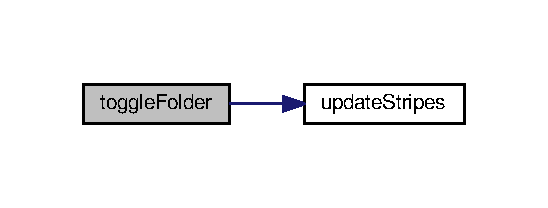
\includegraphics[width=263pt]{dynsections_8js_af244da4527af2d845dca04f5656376cd_cgraph}
\end{center}
\end{figure}


\index{dynsections.\+js@{dynsections.\+js}!toggle\+Inherit@{toggle\+Inherit}}
\index{toggle\+Inherit@{toggle\+Inherit}!dynsections.\+js@{dynsections.\+js}}
\subsubsection[{\texorpdfstring{toggle\+Inherit(id)}{toggleInherit(id)}}]{\setlength{\rightskip}{0pt plus 5cm}function toggle\+Inherit (
\begin{DoxyParamCaption}
\item[{}]{id}
\end{DoxyParamCaption}
)}\hypertarget{dynsections_8js_ac057b640b17ff32af11ced151c9305b4}{}\label{dynsections_8js_ac057b640b17ff32af11ced151c9305b4}


Definition at line 84 of file dynsections.\+js.



Here is the call graph for this function\+:
\nopagebreak
\begin{figure}[H]
\begin{center}
\leavevmode
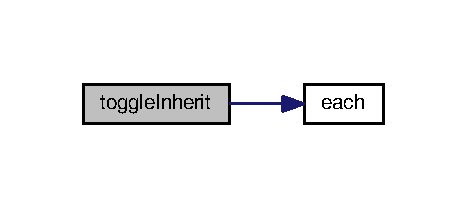
\includegraphics[width=224pt]{dynsections_8js_ac057b640b17ff32af11ced151c9305b4_cgraph}
\end{center}
\end{figure}


\index{dynsections.\+js@{dynsections.\+js}!toggle\+Level@{toggle\+Level}}
\index{toggle\+Level@{toggle\+Level}!dynsections.\+js@{dynsections.\+js}}
\subsubsection[{\texorpdfstring{toggle\+Level(level)}{toggleLevel(level)}}]{\setlength{\rightskip}{0pt plus 5cm}function toggle\+Level (
\begin{DoxyParamCaption}
\item[{}]{level}
\end{DoxyParamCaption}
)}\hypertarget{dynsections_8js_a19f577cc1ba571396a85bb1f48bf4df2}{}\label{dynsections_8js_a19f577cc1ba571396a85bb1f48bf4df2}


Definition at line 28 of file dynsections.\+js.



Here is the call graph for this function\+:
\nopagebreak
\begin{figure}[H]
\begin{center}
\leavevmode
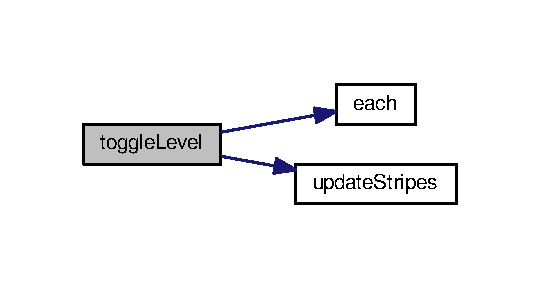
\includegraphics[width=259pt]{dynsections_8js_a19f577cc1ba571396a85bb1f48bf4df2_cgraph}
\end{center}
\end{figure}


\index{dynsections.\+js@{dynsections.\+js}!toggle\+Visibility@{toggle\+Visibility}}
\index{toggle\+Visibility@{toggle\+Visibility}!dynsections.\+js@{dynsections.\+js}}
\subsubsection[{\texorpdfstring{toggle\+Visibility(link\+Obj)}{toggleVisibility(linkObj)}}]{\setlength{\rightskip}{0pt plus 5cm}function toggle\+Visibility (
\begin{DoxyParamCaption}
\item[{}]{link\+Obj}
\end{DoxyParamCaption}
)}\hypertarget{dynsections_8js_a1922c462474df7dfd18741c961d59a25}{}\label{dynsections_8js_a1922c462474df7dfd18741c961d59a25}


Definition at line 1 of file dynsections.\+js.

\index{dynsections.\+js@{dynsections.\+js}!update\+Stripes@{update\+Stripes}}
\index{update\+Stripes@{update\+Stripes}!dynsections.\+js@{dynsections.\+js}}
\subsubsection[{\texorpdfstring{update\+Stripes()}{updateStripes()}}]{\setlength{\rightskip}{0pt plus 5cm}function update\+Stripes (
\begin{DoxyParamCaption}
{}
\end{DoxyParamCaption}
)}\hypertarget{dynsections_8js_a8f7493ad859d4fbf2523917511ee7177}{}\label{dynsections_8js_a8f7493ad859d4fbf2523917511ee7177}


Definition at line 22 of file dynsections.\+js.



Here is the caller graph for this function\+:
\nopagebreak
\begin{figure}[H]
\begin{center}
\leavevmode
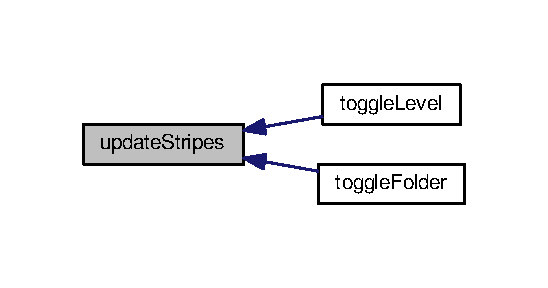
\includegraphics[width=263pt]{dynsections_8js_a8f7493ad859d4fbf2523917511ee7177_icgraph}
\end{center}
\end{figure}



\hypertarget{feature____tests__8c_8js}{}\section{docs/feature\+\_\+\+\_\+tests\+\_\+8c.js File Reference}
\label{feature____tests__8c_8js}\index{docs/feature\+\_\+\+\_\+tests\+\_\+8c.\+js@{docs/feature\+\_\+\+\_\+tests\+\_\+8c.\+js}}
\subsection*{Variables}
\begin{DoxyCompactItemize}
\item 
var \hyperlink{feature____tests__8c_8js_a4441914e36463a1e04ac4be7667056f0}{feature\+\_\+\+\_\+tests\+\_\+8c}
\end{DoxyCompactItemize}


\subsection{Variable Documentation}
\index{feature\+\_\+\+\_\+tests\+\_\+8c.\+js@{feature\+\_\+\+\_\+tests\+\_\+8c.\+js}!feature\+\_\+\+\_\+tests\+\_\+8c@{feature\+\_\+\+\_\+tests\+\_\+8c}}
\index{feature\+\_\+\+\_\+tests\+\_\+8c@{feature\+\_\+\+\_\+tests\+\_\+8c}!feature\+\_\+\+\_\+tests\+\_\+8c.\+js@{feature\+\_\+\+\_\+tests\+\_\+8c.\+js}}
\subsubsection[{\texorpdfstring{feature\+\_\+\+\_\+tests\+\_\+8c}{feature__tests_8c}}]{\setlength{\rightskip}{0pt plus 5cm}var feature\+\_\+\+\_\+tests\+\_\+8c}\hypertarget{feature____tests__8c_8js_a4441914e36463a1e04ac4be7667056f0}{}\label{feature____tests__8c_8js_a4441914e36463a1e04ac4be7667056f0}
{\bfseries Initial value\+:}
\begin{DoxyCode}
=
[
    [ \textcolor{stringliteral}{"main"}, \textcolor{stringliteral}{"feature\_\_tests\_8c.html#a3c04138a5bfe5d72780bb7e82a18e627"}, null ],
    [ \textcolor{stringliteral}{"features"}, \textcolor{stringliteral}{"feature\_\_tests\_8c.html#a1582568e32f689337602a16bf8a5bff0"}, null ]
]
\end{DoxyCode}


Definition at line 1 of file feature\+\_\+\+\_\+tests\+\_\+8c.\+js.


\hypertarget{feature____tests__8cxx_8js}{}\section{docs/feature\+\_\+\+\_\+tests\+\_\+8cxx.js File Reference}
\label{feature____tests__8cxx_8js}\index{docs/feature\+\_\+\+\_\+tests\+\_\+8cxx.\+js@{docs/feature\+\_\+\+\_\+tests\+\_\+8cxx.\+js}}
\subsection*{Variables}
\begin{DoxyCompactItemize}
\item 
var \hyperlink{feature____tests__8cxx_8js_aa0c2967963d427c962b622690ecec17f}{feature\+\_\+\+\_\+tests\+\_\+8cxx}
\end{DoxyCompactItemize}


\subsection{Variable Documentation}
\index{feature\+\_\+\+\_\+tests\+\_\+8cxx.\+js@{feature\+\_\+\+\_\+tests\+\_\+8cxx.\+js}!feature\+\_\+\+\_\+tests\+\_\+8cxx@{feature\+\_\+\+\_\+tests\+\_\+8cxx}}
\index{feature\+\_\+\+\_\+tests\+\_\+8cxx@{feature\+\_\+\+\_\+tests\+\_\+8cxx}!feature\+\_\+\+\_\+tests\+\_\+8cxx.\+js@{feature\+\_\+\+\_\+tests\+\_\+8cxx.\+js}}
\subsubsection[{\texorpdfstring{feature\+\_\+\+\_\+tests\+\_\+8cxx}{feature__tests_8cxx}}]{\setlength{\rightskip}{0pt plus 5cm}var feature\+\_\+\+\_\+tests\+\_\+8cxx}\hypertarget{feature____tests__8cxx_8js_aa0c2967963d427c962b622690ecec17f}{}\label{feature____tests__8cxx_8js_aa0c2967963d427c962b622690ecec17f}
{\bfseries Initial value\+:}
\begin{DoxyCode}
=
[
    [ \textcolor{stringliteral}{"main"}, \textcolor{stringliteral}{"feature\_\_tests\_8cxx.html#a3c04138a5bfe5d72780bb7e82a18e627"}, null ],
    [ \textcolor{stringliteral}{"features"}, \textcolor{stringliteral}{"feature\_\_tests\_8cxx.html#a1582568e32f689337602a16bf8a5bff0"}, null ]
]
\end{DoxyCode}


Definition at line 1 of file feature\+\_\+\+\_\+tests\+\_\+8cxx.\+js.


\hypertarget{files_8js}{}\section{docs/files.js File Reference}
\label{files_8js}\index{docs/files.\+js@{docs/files.\+js}}
\subsection*{Variables}
\begin{DoxyCompactItemize}
\item 
var \hyperlink{files_8js_a0742cac2750bccc2d88ac080fb9daa22}{files}
\end{DoxyCompactItemize}


\subsection{Variable Documentation}
\index{files.\+js@{files.\+js}!files@{files}}
\index{files@{files}!files.\+js@{files.\+js}}
\subsubsection[{\texorpdfstring{files}{files}}]{\setlength{\rightskip}{0pt plus 5cm}var files}\hypertarget{files_8js_a0742cac2750bccc2d88ac080fb9daa22}{}\label{files_8js_a0742cac2750bccc2d88ac080fb9daa22}
{\bfseries Initial value\+:}
\begin{DoxyCode}
=
[
    [ \textcolor{stringliteral}{"build"}, \textcolor{stringliteral}{"dir\_4fef79e7177ba769987a8da36c892c5f.html"}, \textcolor{stringliteral}{"dir\_4fef79e7177ba769987a8da36c892c5f"} ],
    [ \textcolor{stringliteral}{"include"}, \textcolor{stringliteral}{"dir\_d44c64559bbebec7f509842c48db8b23.html"}, \textcolor{stringliteral}{"dir\_d44c64559bbebec7f509842c48db8b23"} ],
    [ \textcolor{stringliteral}{"src"}, \textcolor{stringliteral}{"dir\_68267d1309a1af8e8297ef4c3efbcdba.html"}, \textcolor{stringliteral}{"dir\_68267d1309a1af8e8297ef4c3efbcdba"} ]
]
\end{DoxyCode}


Definition at line 1 of file files.\+js.


\hypertarget{functions__dup_8js}{}\section{docs/functions\+\_\+dup.js File Reference}
\label{functions__dup_8js}\index{docs/functions\+\_\+dup.\+js@{docs/functions\+\_\+dup.\+js}}
\subsection*{Variables}
\begin{DoxyCompactItemize}
\item 
var \hyperlink{functions__dup_8js_a8eb2e04e78e0cae8380f93a505246352}{functions\+\_\+dup}
\end{DoxyCompactItemize}


\subsection{Variable Documentation}
\index{functions\+\_\+dup.\+js@{functions\+\_\+dup.\+js}!functions\+\_\+dup@{functions\+\_\+dup}}
\index{functions\+\_\+dup@{functions\+\_\+dup}!functions\+\_\+dup.\+js@{functions\+\_\+dup.\+js}}
\subsubsection[{\texorpdfstring{functions\+\_\+dup}{functions_dup}}]{\setlength{\rightskip}{0pt plus 5cm}var functions\+\_\+dup}\hypertarget{functions__dup_8js_a8eb2e04e78e0cae8380f93a505246352}{}\label{functions__dup_8js_a8eb2e04e78e0cae8380f93a505246352}
{\bfseries Initial value\+:}
\begin{DoxyCode}
=
[
    [ \textcolor{stringliteral}{"a"}, \textcolor{stringliteral}{"functions.html"}, null ],
    [ \textcolor{stringliteral}{"b"}, \textcolor{stringliteral}{"functions\_b.html"}, null ],
    [ \textcolor{stringliteral}{"c"}, \textcolor{stringliteral}{"functions\_c.html"}, null ],
    [ \textcolor{stringliteral}{"d"}, \textcolor{stringliteral}{"functions\_d.html"}, null ],
    [ \textcolor{stringliteral}{"e"}, \textcolor{stringliteral}{"functions\_e.html"}, null ],
    [ \textcolor{stringliteral}{"f"}, \textcolor{stringliteral}{"functions\_f.html"}, null ],
    [ \textcolor{stringliteral}{"g"}, \textcolor{stringliteral}{"functions\_g.html"}, null ],
    [ \textcolor{stringliteral}{"h"}, \textcolor{stringliteral}{"functions\_h.html"}, null ],
    [ \textcolor{stringliteral}{"i"}, \textcolor{stringliteral}{"functions\_i.html"}, null ],
    [ \textcolor{stringliteral}{"l"}, \textcolor{stringliteral}{"functions\_l.html"}, null ],
    [ \textcolor{stringliteral}{"m"}, \textcolor{stringliteral}{"functions\_m.html"}, null ],
    [ \textcolor{stringliteral}{"n"}, \textcolor{stringliteral}{"functions\_n.html"}, null ],
    [ \textcolor{stringliteral}{"o"}, \textcolor{stringliteral}{"functions\_o.html"}, null ],
    [ \textcolor{stringliteral}{"p"}, \textcolor{stringliteral}{"functions\_p.html"}, null ],
    [ \textcolor{stringliteral}{"q"}, \textcolor{stringliteral}{"functions\_q.html"}, null ],
    [ \textcolor{stringliteral}{"r"}, \textcolor{stringliteral}{"functions\_r.html"}, null ],
    [ \textcolor{stringliteral}{"s"}, \textcolor{stringliteral}{"functions\_s.html"}, null ],
    [ \textcolor{stringliteral}{"t"}, \textcolor{stringliteral}{"functions\_t.html"}, null ],
    [ \textcolor{stringliteral}{"u"}, \textcolor{stringliteral}{"functions\_u.html"}, null ],
    [ \textcolor{stringliteral}{"v"}, \textcolor{stringliteral}{"functions\_v.html"}, null ],
    [ \textcolor{stringliteral}{"w"}, \textcolor{stringliteral}{"functions\_w.html"}, null ],
    [ \textcolor{stringliteral}{"x"}, \textcolor{stringliteral}{"functions\_x.html"}, null ],
    [ \textcolor{stringliteral}{"y"}, \textcolor{stringliteral}{"functions\_y.html"}, null ],
    [ \textcolor{stringliteral}{"z"}, \textcolor{stringliteral}{"functions\_z.html"}, null ],
    [ \textcolor{stringliteral}{"~"}, \textcolor{stringliteral}{"functions\_0x7e.html"}, null ]
]
\end{DoxyCode}


Definition at line 1 of file functions\+\_\+dup.\+js.


\hypertarget{generate____cached____setup__8py_8js}{}\section{docs/generate\+\_\+\+\_\+cached\+\_\+\+\_\+setup\+\_\+8py.js File Reference}
\label{generate____cached____setup__8py_8js}\index{docs/generate\+\_\+\+\_\+cached\+\_\+\+\_\+setup\+\_\+8py.\+js@{docs/generate\+\_\+\+\_\+cached\+\_\+\+\_\+setup\+\_\+8py.\+js}}
\subsection*{Variables}
\begin{DoxyCompactItemize}
\item 
var \hyperlink{generate____cached____setup__8py_8js_a415f3bf74b010fccf1e865ee6b2f40db}{generate\+\_\+\+\_\+cached\+\_\+\+\_\+setup\+\_\+8py}
\end{DoxyCompactItemize}


\subsection{Variable Documentation}
\index{generate\+\_\+\+\_\+cached\+\_\+\+\_\+setup\+\_\+8py.\+js@{generate\+\_\+\+\_\+cached\+\_\+\+\_\+setup\+\_\+8py.\+js}!generate\+\_\+\+\_\+cached\+\_\+\+\_\+setup\+\_\+8py@{generate\+\_\+\+\_\+cached\+\_\+\+\_\+setup\+\_\+8py}}
\index{generate\+\_\+\+\_\+cached\+\_\+\+\_\+setup\+\_\+8py@{generate\+\_\+\+\_\+cached\+\_\+\+\_\+setup\+\_\+8py}!generate\+\_\+\+\_\+cached\+\_\+\+\_\+setup\+\_\+8py.\+js@{generate\+\_\+\+\_\+cached\+\_\+\+\_\+setup\+\_\+8py.\+js}}
\subsubsection[{\texorpdfstring{generate\+\_\+\+\_\+cached\+\_\+\+\_\+setup\+\_\+8py}{generate__cached__setup_8py}}]{\setlength{\rightskip}{0pt plus 5cm}var generate\+\_\+\+\_\+cached\+\_\+\+\_\+setup\+\_\+8py}\hypertarget{generate____cached____setup__8py_8js_a415f3bf74b010fccf1e865ee6b2f40db}{}\label{generate____cached____setup__8py_8js_a415f3bf74b010fccf1e865ee6b2f40db}
{\bfseries Initial value\+:}
\begin{DoxyCode}
=
[
    [ \textcolor{stringliteral}{"code"}, \textcolor{stringliteral}{"generate\_\_cached\_\_setup\_8py.html#a52601295006f2366a311c4453d8f2f2e"}, null ],
    [ \textcolor{stringliteral}{"mode"}, \textcolor{stringliteral}{"generate\_\_cached\_\_setup\_8py.html#a10081e5abedae9bd46dd91202096e789"}, null ],
    [ \textcolor{stringliteral}{"output\_filename"}, \textcolor{stringliteral}{"generate\_\_cached\_\_setup\_8py.html#a0265aee5075ee1eb701ff69c98ad6793"}, null ],
    [ \textcolor{stringliteral}{"python\_path"}, \textcolor{stringliteral}{"generate\_\_cached\_\_setup\_8py.html#a72579fd01529a79bab20d99291889d3f"}, null ]
]
\end{DoxyCode}


Definition at line 1 of file generate\+\_\+\+\_\+cached\+\_\+\+\_\+setup\+\_\+8py.\+js.


\hypertarget{hierarchy_8js}{}\section{docs/hierarchy.js File Reference}
\label{hierarchy_8js}\index{docs/hierarchy.\+js@{docs/hierarchy.\+js}}
\subsection*{Variables}
\begin{DoxyCompactItemize}
\item 
var \hyperlink{hierarchy_8js_ad9447ad30669c42ccb861cbe36a18f6b}{hierarchy}
\end{DoxyCompactItemize}


\subsection{Variable Documentation}
\index{hierarchy.\+js@{hierarchy.\+js}!hierarchy@{hierarchy}}
\index{hierarchy@{hierarchy}!hierarchy.\+js@{hierarchy.\+js}}
\subsubsection[{\texorpdfstring{hierarchy}{hierarchy}}]{\setlength{\rightskip}{0pt plus 5cm}var hierarchy}\hypertarget{hierarchy_8js_ad9447ad30669c42ccb861cbe36a18f6b}{}\label{hierarchy_8js_ad9447ad30669c42ccb861cbe36a18f6b}
{\bfseries Initial value\+:}
\begin{DoxyCode}
=
[
    [ \textcolor{stringliteral}{"Chaser"}, \textcolor{stringliteral}{"class\_chaser.html"}, null ],
    [ \textcolor{stringliteral}{"FieldParams"}, \textcolor{stringliteral}{"struct\_field\_params.html"}, null ],
    [ \textcolor{stringliteral}{"GridField"}, \textcolor{stringliteral}{"struct\_grid\_field.html"}, null ],
    [ \textcolor{stringliteral}{"Node< T >"}, \textcolor{stringliteral}{"struct\_node.html"}, null ],
    [ \textcolor{stringliteral}{"ObjectsHandler"}, \textcolor{stringliteral}{"class\_objects\_handler.html"}, null ],
    [ \textcolor{stringliteral}{"Preplanner"}, \textcolor{stringliteral}{"class\_preplanner.html"}, null ],
    [ \textcolor{stringliteral}{"chaser::PreplannerParams"}, \textcolor{stringliteral}{"structchaser\_1\_1\_preplanner\_params.html"}, null ],
    [ \textcolor{stringliteral}{"QMainWindow"}, null, [
      [ \textcolor{stringliteral}{"MainWindow"}, \textcolor{stringliteral}{"class\_main\_window.html"}, null ]
    ] ],
    [ \textcolor{stringliteral}{"QThread"}, null, [
      [ \textcolor{stringliteral}{"QNode"}, \textcolor{stringliteral}{"class\_q\_node.html"}, null ]
    ] ],
    [ \textcolor{stringliteral}{"SmoothPlanner"}, \textcolor{stringliteral}{"class\_smooth\_planner.html"}, null ],
    [ \textcolor{stringliteral}{"chaser::SmoothplannerParams"}, \textcolor{stringliteral}{"structchaser\_1\_1\_smoothplanner\_params.html"}, null ],
    [ \textcolor{stringliteral}{"TargetManager"}, \textcolor{stringliteral}{"class\_target\_manager.html"}, null ],
    [ \textcolor{stringliteral}{"Ui\_MainWindow"}, \textcolor{stringliteral}{"class\_ui\_\_\_main\_window.html"}, [
      [ \textcolor{stringliteral}{"Ui::MainWindow"}, \textcolor{stringliteral}{"class\_ui\_1\_1\_main\_window.html"}, null ]
    ] ],
    [ \textcolor{stringliteral}{"Wrapper"}, \textcolor{stringliteral}{"class\_wrapper.html"}, null ]
]
\end{DoxyCode}


Definition at line 1 of file hierarchy.\+js.


\hypertarget{jquery_8js}{}\section{docs/jquery.js File Reference}
\label{jquery_8js}\index{docs/jquery.\+js@{docs/jquery.\+js}}
\subsection*{Functions}
\begin{DoxyCompactItemize}
\item 
\hyperlink{jquery_8js_a2fa551895933fae935a0a6b87282241d}{b} \hyperlink{jquery_8js_a5fb206c91c64d1be35fde236706eab86}{extend} (\{css\+Hooks\+:\{opacity\+:\{get\+:function(bw, bv)\{\hyperlink{jquery_8js_a42cbfadee2b4749e8f699ea8d745a0e4}{if}(bv)\{var e=\hyperlink{jquery_8js_adc18d83abfd9f87d396e8fd6b6ac0fe1}{Z}(bw,\char`\"{}opacity\char`\"{},\char`\"{}opacity\char`\"{});return e===\char`\"{}\char`\"{}?\char`\"{}1\char`\"{}\+:e\}else\{return bw.\+style.\+opacity\}\}\}\}, css\+Number\+:\{fill\+Opacity\+:true, font\+Weight\+:true, line\+Height\+:true, opacity\+:true, orphans\+:true, widows\+:true, z\+Index\+:true, zoom\+:true\}, css\+Props\+:\{\char`\"{}float\char`\"{}\+:b.\+support.\+css\+Float?\char`\"{}css\+Float\char`\"{}\+:\char`\"{}style\+Float\char`\"{}\}, style\+:function(bx, bw, bD, by)\{\hyperlink{jquery_8js_a42cbfadee2b4749e8f699ea8d745a0e4}{if}(!bx$\vert$$\vert$bx.\+node\+Type===3$\vert$$\vert$bx.\+node\+Type===8$\vert$$\vert$!bx.\+style)\{return\}var bB, bC, bz=b.\+camel\+Case(bw), bv=bx.\+style, bE=b.\+css\+Hooks\mbox{[}bz\mbox{]};bw=b.\+css\+Props\mbox{[}bz\mbox{]}$\vert$$\vert$bz;\hyperlink{jquery_8js_a42cbfadee2b4749e8f699ea8d745a0e4}{if}(b\+D!==\hyperlink{jquery_8js_a38ee4c0b5f4fe2a18d0c783af540d253}{L})\{bC=typeof bD;\hyperlink{jquery_8js_a42cbfadee2b4749e8f699ea8d745a0e4}{if}(bC===\char`\"{}string\char`\"{}\&\&(bB=I.\+exec(bD)))\{bD=(+(bB\mbox{[}1\mbox{]}+1)$\ast$+bB\mbox{[}2\mbox{]})+parse\+Float(\hyperlink{jquery_8js_a89ad527fcd82c01ebb587332f5b4fcd4}{b.\+css}(bx, bw));bC=\char`\"{}number\char`\"{}\}if(bD==null$\vert$$\vert$bC===\char`\"{}number\char`\"{}\&\&is\+NaN(bD))\{return\}\hyperlink{jquery_8js_a42cbfadee2b4749e8f699ea8d745a0e4}{if}(bC===\char`\"{}number\char`\"{}\&\&!b.\+css\+Number\mbox{[}bz\mbox{]})\{bD+=\char`\"{}px\char`\"{}\}if(!bE$\vert$$\vert$!(\char`\"{}set\char`\"{}in bE)$\vert$$\vert$(bD=b\+E.\+set(bx, bD))!==\hyperlink{jquery_8js_a38ee4c0b5f4fe2a18d0c783af540d253}{L})\{try\{bv\mbox{[}bw\mbox{]}=bD\}catch(bA)\{\}\}\}else\{\hyperlink{jquery_8js_a42cbfadee2b4749e8f699ea8d745a0e4}{if}(bE \&\&\char`\"{}get\char`\"{}in bE \&\&(bB=b\+E.\+get(bx, false, by))!==\hyperlink{jquery_8js_a38ee4c0b5f4fe2a18d0c783af540d253}{L})\{return bB\}return bv\mbox{[}bw\mbox{]}\}\}, css\+:function(by, bx, bv)\{var bw, e;bx=b.\+camel\+Case(bx);e=b.\+css\+Hooks\mbox{[}bx\mbox{]};bx=b.\+css\+Props\mbox{[}bx\mbox{]}$\vert$$\vert$bx;\hyperlink{jquery_8js_a42cbfadee2b4749e8f699ea8d745a0e4}{if}(bx===\char`\"{}css\+Float\char`\"{})\{bx=\char`\"{}float\char`\"{}\}if(e \&\&\char`\"{}get\char`\"{}in e \&\&(bw=e.\+get(by, true, bv))!==\hyperlink{jquery_8js_a38ee4c0b5f4fe2a18d0c783af540d253}{L})\{return bw\}else\{\hyperlink{jquery_8js_a42cbfadee2b4749e8f699ea8d745a0e4}{if}(\hyperlink{jquery_8js_adc18d83abfd9f87d396e8fd6b6ac0fe1}{Z})\{return \hyperlink{jquery_8js_adc18d83abfd9f87d396e8fd6b6ac0fe1}{Z}(by, bx)\}\}\}, swap\+:function(bx, bw, by)\{var e=\{\};for(var bv in bw)\{e\mbox{[}bv\mbox{]}=bx.\+style\mbox{[}bv\mbox{]};bx.\+style\mbox{[}bv\mbox{]}=bw\mbox{[}bv\mbox{]}\}by.\+call(bx);for(bv in bw)\{bx.\+style\mbox{[}bv\mbox{]}=e\mbox{[}bv\mbox{]}\}\}\})
\item 
\hyperlink{jquery_8js_a2fa551895933fae935a0a6b87282241d}{b} \hyperlink{jquery_8js_a871ff39db627c54c710a3e9909b8234c}{each} (\mbox{[}\char`\"{}height\char`\"{},\char`\"{}width\char`\"{}\mbox{]}, function(bv, e)\{b.\+css\+Hooks\mbox{[}e\mbox{]}=\{get\+:function(by, bx, bw)\{var bz;\hyperlink{jquery_8js_a42cbfadee2b4749e8f699ea8d745a0e4}{if}(bx)\{\hyperlink{jquery_8js_a42cbfadee2b4749e8f699ea8d745a0e4}{if}(by.\+offset\+Width!==0)\{return \hyperlink{jquery_8js_a2335e57f79b6acfb6de59c235dc8a83e}{p}(by, e, bw)\}else\{b.\+swap(by, a7, function()\{bz=\hyperlink{jquery_8js_a2335e57f79b6acfb6de59c235dc8a83e}{p}(by, e, bw)\})\}return bz\}\}, set\+:function(bw, bx)\{\hyperlink{jquery_8js_a42cbfadee2b4749e8f699ea8d745a0e4}{if}(bc.\+test(bx))\{bx=parse\+Float(bx);\hyperlink{jquery_8js_a42cbfadee2b4749e8f699ea8d745a0e4}{if}(bx $>$=0)\{return bx+\char`\"{}px\char`\"{}\}\}else\{return bx\}\}\}\})
\item 
\hyperlink{jquery_8js_a9db6d45a025ad692282fe23e69eeba43}{if} (!b.\+support.\+opacity)
\item 
\hyperlink{jquery_8js_a2fa551895933fae935a0a6b87282241d}{b} (function()\{\hyperlink{jquery_8js_a42cbfadee2b4749e8f699ea8d745a0e4}{if}(!b.\+support.\+reliable\+Margin\+Right)\{b.\+css\+Hooks.\+margin\+Right=\{get\+:function(bw, bv)\{var e;b.\+swap(bw,\{display\+:\char`\"{}inline-\/block\char`\"{}\}, function()\{\hyperlink{jquery_8js_a42cbfadee2b4749e8f699ea8d745a0e4}{if}(bv)\{e=\hyperlink{jquery_8js_adc18d83abfd9f87d396e8fd6b6ac0fe1}{Z}(bw,\char`\"{}margin-\/right\char`\"{},\char`\"{}margin\+Right\char`\"{})\}else\{e=bw.\+style.\+margin\+Right\}\});return e\}\}\}\})
\item 
\hyperlink{jquery_8js_a30d3d2cd5b567c9f31b2aa30b9cb3bb8}{if} (av.\+default\+View \&\&av.\+default\+View.\+get\+Computed\+Style)
\item 
\hyperlink{jquery_8js_a2c54bd8ed7482e89d19331ba61fe221c}{if} (av.\+document\+Element.\+current\+Style)
\item 
function \hyperlink{jquery_8js_a2335e57f79b6acfb6de59c235dc8a83e}{p} (by, bw, bv)
\item 
\hyperlink{jquery_8js_a42cbfadee2b4749e8f699ea8d745a0e4}{if} (b.\+expr \&\&b.\+expr.\+filters)
\end{DoxyCompactItemize}
\subsection*{Variables}
\begin{DoxyCompactItemize}
\item 
function \hyperlink{jquery_8js_a1d6558865876e1c8cca029fce41a4bdb}{bb}
\item 
function \hyperlink{jquery_8js_a38ee4c0b5f4fe2a18d0c783af540d253}{L} \{var av=bb.\+document,bu=bb.\+navigator,bl=bb.\+location
\item 
var \hyperlink{jquery_8js_aa4026ad5544b958e54ce5e106fa1c805}{b}
\item 
var \hyperlink{jquery_8js_a4fd8ddfab07c8d7c7cae0ab0e052cad3}{au} =/opacity=(\mbox{[}$^\wedge$)\mbox{]}$\ast$)/,z=/(\mbox{[}A-\/\hyperlink{jquery_8js_adc18d83abfd9f87d396e8fd6b6ac0fe1}{Z}\mbox{]}$\vert$$^\wedge$ms)/g,bc=/$^\wedge$-\/?\textbackslash{}d+(?\+:px)?\$/i,bn=/$^\wedge$-\/?\textbackslash{}d/,I=/$^\wedge$(\mbox{[}\textbackslash{}-\/+\mbox{]})=(\mbox{[}\textbackslash{}-\/+.\textbackslash{}de\mbox{]}+)/,a7=\{position\+:\char`\"{}absolute\char`\"{},visibility\+:\char`\"{}hidden\char`\"{},display\+:\char`\"{}block\char`\"{}\},an=\mbox{[}\char`\"{}Left\char`\"{},\char`\"{}Right\char`\"{}\mbox{]},a1=\mbox{[}\char`\"{}Top\char`\"{},\char`\"{}Bottom\char`\"{}\mbox{]},Z,aI,aX
\item 
\hyperlink{jquery_8js_a2fa551895933fae935a0a6b87282241d}{b} fn \hyperlink{jquery_8js_a89ad527fcd82c01ebb587332f5b4fcd4}{css} =function(e,bv)\{\hyperlink{jquery_8js_a42cbfadee2b4749e8f699ea8d745a0e4}{if}(arguments.\+length===2\&\&bv===\hyperlink{jquery_8js_a38ee4c0b5f4fe2a18d0c783af540d253}{L})\{return this\}return b.\+access(this,e,bv,true,function(bx,bw,by)\{return by!==\hyperlink{jquery_8js_a38ee4c0b5f4fe2a18d0c783af540d253}{L}?b.\+style(bx,bw,by)\+:b.\+css(bx,bw)\})\}
\item 
\hyperlink{jquery_8js_a2fa551895933fae935a0a6b87282241d}{b} \hyperlink{jquery_8js_a88b21f8ba3af86d6981b1da520ece33b}{cur\+C\+SS} =\hyperlink{jquery_8js_a89ad527fcd82c01ebb587332f5b4fcd4}{b.\+css}
\item 
\hyperlink{jquery_8js_adc18d83abfd9f87d396e8fd6b6ac0fe1}{Z} =aI$\vert$$\vert$aX
\item 
var \hyperlink{jquery_8js_ab26645c014aa005ecedef329ecf58c99}{k} =/\%20/g
\item 
var \hyperlink{jquery_8js_a6ddf393cc7f9a8828e197bb0d9916c44}{ap} =/\textbackslash{}\mbox{[}\textbackslash{}\mbox{]}\$/
\item 
var \hyperlink{jquery_8js_ae77642f8ef73fb9c20c2a737d956acda}{bs} =/\textbackslash{}r?\textbackslash{}n/g
\item 
var \hyperlink{jquery_8js_af6ee77c71b2c89bdb365145ac5ad1219}{bq} =/\#.$\ast$\$/
\item 
var \hyperlink{jquery_8js_ad223f5fba68c41c1236671ac5c5b0fcb}{aD} =/$^\wedge$(.$\ast$?)\+:\mbox{[} \textbackslash{}t\mbox{]}$\ast$(\mbox{[}$^\wedge$\textbackslash{}r\textbackslash{}n\mbox{]}$\ast$)\textbackslash{}r?\$/mg
\item 
var \hyperlink{jquery_8js_ac87125cdee1a5e57da4ef619af49bc7d}{aZ} =/$^\wedge$(?\+:color$\vert$date$\vert$datetime$\vert$datetime-\/local$\vert$email$\vert$hidden$\vert$month$\vert$number$\vert$password$\vert$range$\vert$search$\vert$tel$\vert$text$\vert$time$\vert$url$\vert$week)\$/i
\item 
var \hyperlink{jquery_8js_a8cc6111a5def3ea889157d13fb9a9672}{aM} =/$^\wedge$(?\+:about$\vert$app$\vert$app\textbackslash{}-\/storage$\vert$.+\textbackslash{}-\/extension$\vert$file$\vert$res$\vert$widget)\+:\$/
\item 
var \hyperlink{jquery_8js_a79eb58dc6cdf0aef563d5dc1ded27df5}{aQ} =/$^\wedge$(?\+:G\+ET$\vert$H\+E\+AD)\$/
\item 
var \hyperlink{jquery_8js_abce695e0af988ece0826d9ad59b8160d}{c}
\end{DoxyCompactItemize}


\subsection{Function Documentation}
\index{jquery.\+js@{jquery.\+js}!b@{b}}
\index{b@{b}!jquery.\+js@{jquery.\+js}}
\subsubsection[{\texorpdfstring{b(function()\lcurly{}if("!b.\+support.\+reliable\+Margin\+Right)\lcurly{}b.\+css\+Hooks.\+margin\+Right=\lcurly{}get\+:function(bw, bv)\lcurly{}var e;b.\+swap(bw,\lcurly{}display\+:""inline-\/block""\rcurly{}, function()\lcurly{}if(bv)\lcurly{}e=\+Z(bw,""margin-\/right"",""margin\+Right"")\rcurly{}else\lcurly{}e=bw.\+style.\+margin\+Right\rcurly{}\rcurly{});return e\rcurly{}\rcurly{}\rcurly{}\rcurly{})}{b(function()\{if(!b.support.reliableMarginRight)\{b.cssHooks.marginRight=\{get:function(bw, bv)\{var e;b.swap(bw,\{display:"inline-block"\}, function()\{if(bv)\{e=Z(bw,"margin-right","marginRight")\}else\{e=bw.style.marginRight\}\});return e\}\}\}\})}}]{\setlength{\rightskip}{0pt plus 5cm}b (
\begin{DoxyParamCaption}
\item[{function()\{{\bf if}(!b.\+support.\+reliable\+Margin\+Right)\{b.\+css\+Hooks.\+margin\+Right=\{get\+:function(bw, bv)\{var e;b.\+swap(bw,\{display\+:\char`\"{}inline-\/block\char`\"{}\}, function()\{{\bf if}(bv)\{e={\bf Z}(bw,\char`\"{}margin-\/right\char`\"{},\char`\"{}margin\+Right\char`\"{})\}else\{e=bw.\+style.\+margin\+Right\}\});return e\}\}\}\}}]{}
\end{DoxyParamCaption}
)}\hypertarget{jquery_8js_a2fa551895933fae935a0a6b87282241d}{}\label{jquery_8js_a2fa551895933fae935a0a6b87282241d}
\index{jquery.\+js@{jquery.\+js}!each@{each}}
\index{each@{each}!jquery.\+js@{jquery.\+js}}
\subsubsection[{\texorpdfstring{each([""height"",""width""], function(bv, e)\lcurly{}b.\+css\+Hooks[e]=\lcurly{}get\+:function(by, bx, bw)\lcurly{}var bz;if(bx)\lcurly{}if(by.\+offset\+Width"!==0)\lcurly{}return p(by, e, bw)\rcurly{}else\lcurly{}b.\+swap(by, a7, function()\lcurly{}bz=p(by, e, bw)\rcurly{})\rcurly{}return bz\rcurly{}\rcurly{}, set\+:function(bw, bx)\lcurly{}if(bc.\+test(bx))\lcurly{}bx=parse\+Float(bx);if(bx $>$=0)\lcurly{}return bx+""px""\rcurly{}\rcurly{}else\lcurly{}return bx\rcurly{}\rcurly{}\rcurly{}\rcurly{})}{each(["height","width"], function(bv, e)\{b.cssHooks[e]=\{get:function(by, bx, bw)\{var bz;if(bx)\{if(by.offsetWidth!==0)\{return p(by, e, bw)\}else\{b.swap(by, a7, function()\{bz=p(by, e, bw)\})\}return bz\}\}, set:function(bw, bx)\{if(bc.test(bx))\{bx=parseFloat(bx);if(bx >=0)\{return bx+"px"\}\}else\{return bx\}\}\}\})}}]{\setlength{\rightskip}{0pt plus 5cm}{\bf b} each (
\begin{DoxyParamCaption}
\item[{function(bv, e)\{b.\+css\+Hooks\mbox{[}e\mbox{]}=\{get\+:function(by, bx, bw)\{var bz;{\bf if}(bx)\{{\bf if}(by.\+offset\+Width!==0)\{return {\bf p}(by, e, bw)\}else\{b.\+swap(by, a7, function()\{bz={\bf p}(by, e, bw)\})\}return bz\}\}, set\+:function(bw, bx)\{{\bf if}(bc.\+test(bx))\{bx=parse\+Float(bx);{\bf if}(bx $>$=0)\{return bx+\char`\"{}px\char`\"{}\}\}else\{return bx\}\}\}\}}]{}
\end{DoxyParamCaption}
)}\hypertarget{jquery_8js_a871ff39db627c54c710a3e9909b8234c}{}\label{jquery_8js_a871ff39db627c54c710a3e9909b8234c}


Here is the caller graph for this function\+:
\nopagebreak
\begin{figure}[H]
\begin{center}
\leavevmode
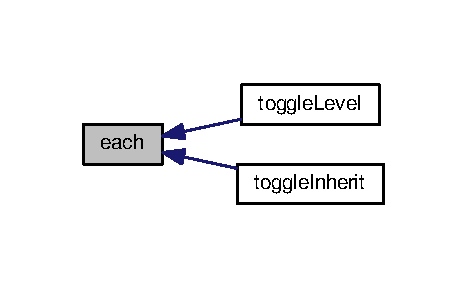
\includegraphics[width=224pt]{jquery_8js_a871ff39db627c54c710a3e9909b8234c_icgraph}
\end{center}
\end{figure}


\index{jquery.\+js@{jquery.\+js}!extend@{extend}}
\index{extend@{extend}!jquery.\+js@{jquery.\+js}}
\subsubsection[{\texorpdfstring{extend(\lcurly{}css\+Hooks\+:\lcurly{}opacity\+:\lcurly{}get\+:function(bw, bv)\lcurly{}if(bv)\lcurly{}var e=\+Z(bw,""opacity"",""opacity"");return e===""""?""1""\+:e\rcurly{}else\lcurly{}return bw.\+style.\+opacity\rcurly{}\rcurly{}\rcurly{}\rcurly{}, css\+Number\+:\lcurly{}fill\+Opacity\+:true, font\+Weight\+:true, line\+Height\+:true, opacity\+:true, orphans\+:true, widows\+:true, z\+Index\+:true, zoom\+:true\rcurly{}, css\+Props\+:\lcurly{}""float""\+:b.\+support.\+css\+Float?""css\+Float""\+:""style\+Float""\rcurly{}, style\+:function(bx, bw, b\+D, by)\lcurly{}if("!bx\texttt{"|}\texttt{"|}bx.\+node\+Type===3\texttt{"|}\texttt{"|}bx.\+node\+Type===8\texttt{"|}\texttt{"|}"!bx.\+style)\lcurly{}return\rcurly{}var b\+B, b\+C, bz=b.\+camel\+Case(bw), bv=bx.\+style, b\+E=b.\+css\+Hooks[bz];bw=b.\+css\+Props[bz]\texttt{"|}\texttt{"|}bz;if(bD"!==\+L)\lcurly{}b\+C=typeof b\+D;if(b\+C===""string""\&\&(b\+B=\+I.\+exec(b\+D)))\lcurly{}b\+D=(+(bB[1]+1)$\ast$+bB[2])+parse\+Float(b.\+css(bx, bw));b\+C=""number""\rcurly{}if(b\+D==null\texttt{"|}\texttt{"|}b\+C===""number""\&\&is\+Na\+N(b\+D))\lcurly{}return\rcurly{}if(b\+C===""number""\&\&"!b.\+css\+Number[bz])\lcurly{}b\+D+=""px""\rcurly{}if("!bE\texttt{"|}\texttt{"|}"!(""set""in b\+E)\texttt{"|}\texttt{"|}(b\+D=b\+E.\+set(bx, b\+D))"!==\+L)\lcurly{}try\lcurly{}bv[bw]=bD\rcurly{}catch(b\+A)\lcurly{}\rcurly{}\rcurly{}\rcurly{}else\lcurly{}if(b\+E \&\&""get""in b\+E \&\&(b\+B=b\+E.\+get(bx, false, by))"!==\+L)\lcurly{}return bB\rcurly{}return bv[bw]\rcurly{}\rcurly{}, css\+:function(by, bx, bv)\lcurly{}var bw, e;bx=b.\+camel\+Case(bx);e=b.\+css\+Hooks[bx];bx=b.\+css\+Props[bx]\texttt{"|}\texttt{"|}bx;if(bx===""css\+Float"")\lcurly{}bx=""float""\rcurly{}if(e \&\&""get""in e \&\&(bw=e.\+get(by, true, bv))"!==\+L)\lcurly{}return bw\rcurly{}else\lcurly{}if(\+Z)\lcurly{}return Z(by, bx)\rcurly{}\rcurly{}\rcurly{}, swap\+:function(bx, bw, by)\lcurly{}var e=\lcurly{}\rcurly{};for(var bv in bw)\lcurly{}e[bv]=bx.\+style[bv];bx.\+style[bv]=bw[bv]\rcurly{}by.\+call(bx);for(bv in bw)\lcurly{}bx.\+style[bv]=e[bv]\rcurly{}\rcurly{}\rcurly{})}{extend(\{cssHooks:\{opacity:\{get:function(bw, bv)\{if(bv)\{var e=Z(bw,"opacity","opacity");return e===""?"1":e\}else\{return bw.style.opacity\}\}\}\}, cssNumber:\{fillOpacity:true, fontWeight:true, lineHeight:true, opacity:true, orphans:true, widows:true, zIndex:true, zoom:true\}, cssProps:\{"float":b.support.cssFloat?"cssFloat":"styleFloat"\}, style:function(bx, bw, bD, by)\{if(!bx||bx.nodeType===3||bx.nodeType===8||!bx.style)\{return\}var bB, bC, bz=b.camelCase(bw), bv=bx.style, bE=b.cssHooks[bz];bw=b.cssProps[bz]||bz;if(bD!==L)\{bC=typeof bD;if(bC==="string"&&(bB=I.exec(bD)))\{bD=(+(bB[1]+1)*+bB[2])+parseFloat(b.css(bx, bw));bC="number"\}if(bD==null||bC==="number"&&isNaN(bD))\{return\}if(bC==="number"&&!b.cssNumber[bz])\{bD+="px"\}if(!bE||!("set"in bE)||(bD=bE.set(bx, bD))!==L)\{try\{bv[bw]=bD\}catch(bA)\{\}\}\}else\{if(bE &&"get"in bE &&(bB=bE.get(bx, false, by))!==L)\{return bB\}return bv[bw]\}\}, css:function(by, bx, bv)\{var bw, e;bx=b.camelCase(bx);e=b.cssHooks[bx];bx=b.cssProps[bx]||bx;if(bx==="cssFloat")\{bx="float"\}if(e &&"get"in e &&(bw=e.get(by, true, bv))!==L)\{return bw\}else\{if(Z)\{return Z(by, bx)\}\}\}, swap:function(bx, bw, by)\{var e=\{\};for(var bv in bw)\{e[bv]=bx.style[bv];bx.style[bv]=bw[bv]\}by.call(bx);for(bv in bw)\{bx.style[bv]=e[bv]\}\}\})}}]{\setlength{\rightskip}{0pt plus 5cm}{\bf b} extend (
\begin{DoxyParamCaption}
\item[{\{css\+Hooks\+:\{opacity\+:\{get\+:function(bw, bv)\{{\bf if}(bv)\{var e={\bf Z}(bw,\char`\"{}opacity\char`\"{},\char`\"{}opacity\char`\"{});return e===\char`\"{}\char`\"{}?\char`\"{}1\char`\"{}\+:e\}else\{return bw.\+style.\+opacity\}\}\}\}, css\+Number\+:\{fill\+Opacity\+:true, font\+Weight\+:true, line\+Height\+:true, opacity\+:true, orphans\+:true, widows\+:true, z\+Index\+:true, zoom\+:true\}, css\+Props\+:\{\char`\"{}float\char`\"{}\+:b.\+support.\+css\+Float?\char`\"{}css\+Float\char`\"{}\+:\char`\"{}style\+Float\char`\"{}\}, style\+:function(bx, bw, bD, by)\{{\bf if}(!bx$\vert$$\vert$bx.\+node\+Type===3$\vert$$\vert$bx.\+node\+Type===8$\vert$$\vert$!bx.\+style)\{return\}var bB, bC, bz=b.\+camel\+Case(bw), bv=bx.\+style, bE=b.\+css\+Hooks\mbox{[}bz\mbox{]};bw=b.\+css\+Props\mbox{[}bz\mbox{]}$\vert$$\vert$bz;{\bf if}(b\+D!=={\bf L})\{bC=typeof bD;{\bf if}(bC===\char`\"{}string\char`\"{}\&\&(bB=I.\+exec(bD)))\{bD=(+(bB\mbox{[}1\mbox{]}+1)$\ast$+bB\mbox{[}2\mbox{]})+parse\+Float({\bf b.\+css}(bx, bw));bC=\char`\"{}number\char`\"{}\}if(bD==null$\vert$$\vert$bC===\char`\"{}number\char`\"{}\&\&is\+NaN(bD))\{return\}{\bf if}(bC===\char`\"{}number\char`\"{}\&\&!b.\+css\+Number\mbox{[}bz\mbox{]})\{bD+=\char`\"{}px\char`\"{}\}if(!bE$\vert$$\vert$!(\char`\"{}set\char`\"{}in bE)$\vert$$\vert$(bD=b\+E.\+set(bx, bD))!=={\bf L})\{try\{bv\mbox{[}bw\mbox{]}=bD\}catch(bA)\{\}\}\}else\{{\bf if}(bE \&\&\char`\"{}get\char`\"{}in bE \&\&(bB=b\+E.\+get(bx, false, by))!=={\bf L})\{return bB\}return bv\mbox{[}bw\mbox{]}\}\}, css\+:function(by, bx, bv)\{var bw, e;bx=b.\+camel\+Case(bx);e=b.\+css\+Hooks\mbox{[}bx\mbox{]};bx=b.\+css\+Props\mbox{[}bx\mbox{]}$\vert$$\vert$bx;{\bf if}(bx===\char`\"{}css\+Float\char`\"{})\{bx=\char`\"{}float\char`\"{}\}if(e \&\&\char`\"{}get\char`\"{}in e \&\&(bw=e.\+get(by, true, bv))!=={\bf L})\{return bw\}else\{{\bf if}({\bf Z})\{return {\bf Z}(by, bx)\}\}\}, swap\+:function(bx, bw, by)\{var e=\{\};for(var bv in bw)\{e\mbox{[}bv\mbox{]}=bx.\+style\mbox{[}bv\mbox{]};bx.\+style\mbox{[}bv\mbox{]}=bw\mbox{[}bv\mbox{]}\}by.\+call(bx);for(bv in bw)\{bx.\+style\mbox{[}bv\mbox{]}=e\mbox{[}bv\mbox{]}\}\}\}}]{}
\end{DoxyParamCaption}
)}\hypertarget{jquery_8js_a5fb206c91c64d1be35fde236706eab86}{}\label{jquery_8js_a5fb206c91c64d1be35fde236706eab86}
\index{jquery.\+js@{jquery.\+js}!if@{if}}
\index{if@{if}!jquery.\+js@{jquery.\+js}}
\subsubsection[{\texorpdfstring{if(av.\+document\+Element.\+current\+Style)}{if(av.documentElement.currentStyle)}}]{\setlength{\rightskip}{0pt plus 5cm}if (
\begin{DoxyParamCaption}
\item[{av.\+document\+Element.}]{current\+Style}
\end{DoxyParamCaption}
)}\hypertarget{jquery_8js_a2c54bd8ed7482e89d19331ba61fe221c}{}\label{jquery_8js_a2c54bd8ed7482e89d19331ba61fe221c}


Definition at line 23 of file jquery.\+js.

\index{jquery.\+js@{jquery.\+js}!if@{if}}
\index{if@{if}!jquery.\+js@{jquery.\+js}}
\subsubsection[{\texorpdfstring{if(av.\+default\+View \&\&av.\+default\+View.\+get\+Computed\+Style)}{if(av.defaultView &&av.defaultView.getComputedStyle)}}]{\setlength{\rightskip}{0pt plus 5cm}if (
\begin{DoxyParamCaption}
\item[{av.\+default\+View \&\&av.\+default\+View.}]{get\+Computed\+Style}
\end{DoxyParamCaption}
)}\hypertarget{jquery_8js_a30d3d2cd5b567c9f31b2aa30b9cb3bb8}{}\label{jquery_8js_a30d3d2cd5b567c9f31b2aa30b9cb3bb8}


Definition at line 23 of file jquery.\+js.

\index{jquery.\+js@{jquery.\+js}!if@{if}}
\index{if@{if}!jquery.\+js@{jquery.\+js}}
\subsubsection[{\texorpdfstring{if(b.\+expr \&\&b.\+expr.\+filters)}{if(b.expr &&b.expr.filters)}}]{\setlength{\rightskip}{0pt plus 5cm}if (
\begin{DoxyParamCaption}
\item[{b.\+expr \&\&b.\+expr.}]{filters}
\end{DoxyParamCaption}
)}\hypertarget{jquery_8js_a42cbfadee2b4749e8f699ea8d745a0e4}{}\label{jquery_8js_a42cbfadee2b4749e8f699ea8d745a0e4}


Definition at line 23 of file jquery.\+js.

\index{jquery.\+js@{jquery.\+js}!if@{if}}
\index{if@{if}!jquery.\+js@{jquery.\+js}}
\subsubsection[{\texorpdfstring{if("!b.\+support.\+opacity)}{if(!b.support.opacity)}}]{\setlength{\rightskip}{0pt plus 5cm}if (
\begin{DoxyParamCaption}
\item[{!b.\+support.}]{opacity}
\end{DoxyParamCaption}
)}\hypertarget{jquery_8js_a9db6d45a025ad692282fe23e69eeba43}{}\label{jquery_8js_a9db6d45a025ad692282fe23e69eeba43}


Definition at line 23 of file jquery.\+js.



Here is the caller graph for this function\+:
\nopagebreak
\begin{figure}[H]
\begin{center}
\leavevmode
\includegraphics[width=226pt]{jquery_8js_a9db6d45a025ad692282fe23e69eeba43_icgraph}
\end{center}
\end{figure}


\index{jquery.\+js@{jquery.\+js}!p@{p}}
\index{p@{p}!jquery.\+js@{jquery.\+js}}
\subsubsection[{\texorpdfstring{p(by, bw, bv)}{p(by, bw, bv)}}]{\setlength{\rightskip}{0pt plus 5cm}function p (
\begin{DoxyParamCaption}
\item[{}]{by, }
\item[{}]{bw, }
\item[{}]{bv}
\end{DoxyParamCaption}
)}\hypertarget{jquery_8js_a2335e57f79b6acfb6de59c235dc8a83e}{}\label{jquery_8js_a2335e57f79b6acfb6de59c235dc8a83e}


Definition at line 23 of file jquery.\+js.



\subsection{Variable Documentation}
\index{jquery.\+js@{jquery.\+js}!aD@{aD}}
\index{aD@{aD}!jquery.\+js@{jquery.\+js}}
\subsubsection[{\texorpdfstring{aD}{aD}}]{\setlength{\rightskip}{0pt plus 5cm}var aD =/$^\wedge$(.$\ast$?)\+:\mbox{[} \textbackslash{}t\mbox{]}$\ast$(\mbox{[}$^\wedge$\textbackslash{}r\textbackslash{}n\mbox{]}$\ast$)\textbackslash{}r?\$/mg}\hypertarget{jquery_8js_ad223f5fba68c41c1236671ac5c5b0fcb}{}\label{jquery_8js_ad223f5fba68c41c1236671ac5c5b0fcb}


Definition at line 23 of file jquery.\+js.

\index{jquery.\+js@{jquery.\+js}!aM@{aM}}
\index{aM@{aM}!jquery.\+js@{jquery.\+js}}
\subsubsection[{\texorpdfstring{aM}{aM}}]{\setlength{\rightskip}{0pt plus 5cm}var aM =/$^\wedge$(?\+:about$\vert$app$\vert$app\textbackslash{}-\/storage$\vert$.+\textbackslash{}-\/extension$\vert$file$\vert$res$\vert$widget)\+:\$/}\hypertarget{jquery_8js_a8cc6111a5def3ea889157d13fb9a9672}{}\label{jquery_8js_a8cc6111a5def3ea889157d13fb9a9672}


Definition at line 23 of file jquery.\+js.

\index{jquery.\+js@{jquery.\+js}!ap@{ap}}
\index{ap@{ap}!jquery.\+js@{jquery.\+js}}
\subsubsection[{\texorpdfstring{ap}{ap}}]{\setlength{\rightskip}{0pt plus 5cm}var ap =/\textbackslash{}\mbox{[}\textbackslash{}\mbox{]}\$/}\hypertarget{jquery_8js_a6ddf393cc7f9a8828e197bb0d9916c44}{}\label{jquery_8js_a6ddf393cc7f9a8828e197bb0d9916c44}


Definition at line 23 of file jquery.\+js.

\index{jquery.\+js@{jquery.\+js}!aQ@{aQ}}
\index{aQ@{aQ}!jquery.\+js@{jquery.\+js}}
\subsubsection[{\texorpdfstring{aQ}{aQ}}]{\setlength{\rightskip}{0pt plus 5cm}var aQ =/$^\wedge$(?\+:G\+ET$\vert$H\+E\+AD)\$/}\hypertarget{jquery_8js_a79eb58dc6cdf0aef563d5dc1ded27df5}{}\label{jquery_8js_a79eb58dc6cdf0aef563d5dc1ded27df5}


Definition at line 23 of file jquery.\+js.

\index{jquery.\+js@{jquery.\+js}!au@{au}}
\index{au@{au}!jquery.\+js@{jquery.\+js}}
\subsubsection[{\texorpdfstring{au}{au}}]{\setlength{\rightskip}{0pt plus 5cm}var au =/opacity=(\mbox{[}$^\wedge$)\mbox{]}$\ast$)/,z=/(\mbox{[}A-\/{\bf Z}\mbox{]}$\vert$$^\wedge$ms)/g,bc=/$^\wedge$-\/?\textbackslash{}d+(?\+:px)?\$/i,bn=/$^\wedge$-\/?\textbackslash{}d/,I=/$^\wedge$(\mbox{[}\textbackslash{}-\/+\mbox{]})=(\mbox{[}\textbackslash{}-\/+.\textbackslash{}de\mbox{]}+)/,a7=\{position\+:\char`\"{}absolute\char`\"{},visibility\+:\char`\"{}hidden\char`\"{},display\+:\char`\"{}block\char`\"{}\},an=\mbox{[}\char`\"{}Left\char`\"{},\char`\"{}Right\char`\"{}\mbox{]},a1=\mbox{[}\char`\"{}Top\char`\"{},\char`\"{}Bottom\char`\"{}\mbox{]},Z,aI,aX}\hypertarget{jquery_8js_a4fd8ddfab07c8d7c7cae0ab0e052cad3}{}\label{jquery_8js_a4fd8ddfab07c8d7c7cae0ab0e052cad3}


Definition at line 23 of file jquery.\+js.

\index{jquery.\+js@{jquery.\+js}!aZ@{aZ}}
\index{aZ@{aZ}!jquery.\+js@{jquery.\+js}}
\subsubsection[{\texorpdfstring{aZ}{aZ}}]{\setlength{\rightskip}{0pt plus 5cm}var aZ =/$^\wedge$(?\+:color$\vert$date$\vert$datetime$\vert$datetime-\/local$\vert$email$\vert$hidden$\vert$month$\vert$number$\vert$password$\vert$range$\vert$search$\vert$tel$\vert$text$\vert$time$\vert$url$\vert$week)\$/i}\hypertarget{jquery_8js_ac87125cdee1a5e57da4ef619af49bc7d}{}\label{jquery_8js_ac87125cdee1a5e57da4ef619af49bc7d}


Definition at line 23 of file jquery.\+js.

\index{jquery.\+js@{jquery.\+js}!b@{b}}
\index{b@{b}!jquery.\+js@{jquery.\+js}}
\subsubsection[{\texorpdfstring{b}{b}}]{\setlength{\rightskip}{0pt plus 5cm}var b}\hypertarget{jquery_8js_aa4026ad5544b958e54ce5e106fa1c805}{}\label{jquery_8js_aa4026ad5544b958e54ce5e106fa1c805}
{\bfseries Initial value\+:}
\begin{DoxyCode}
=(\textcolor{keyword}{function}()\{var bF=\textcolor{keyword}{function}(b0,b1)\{\textcolor{keywordflow}{return} \textcolor{keyword}{new} bF.fn.init(b0,b1,bD)\},bU=\hyperlink{jquery_8js_a1d6558865876e1c8cca029fce41a4bdb}{bb}.jQuery,bH=
      \hyperlink{jquery_8js_a1d6558865876e1c8cca029fce41a4bdb}{bb}.$,bD,bY=/^(?:[^#<]*(<[\(\backslash\)w\(\backslash\)W]+>)[^>]*$|#([\(\backslash\)w\(\backslash\)-]*)$)/,bM=/\(\backslash\)S/,bI=/^\(\backslash\)s+/,bE=/\(\backslash\)s+$/,bA=/^<(\(\backslash\)w+)\(\backslash\)s*\(\backslash\)/?>(?:<\(\backslash\)
      /\(\backslash\)1>)?$/,bN=/^[\(\backslash\)],:\{\}\(\backslash\)s]*$/,bW=/\(\backslash\)\(\backslash\)(?:[\textcolor{stringliteral}{"\(\backslash\)\(\backslash\)\(\backslash\)/bfnrt]|u[0-9a-fA-F]\{4\})/g,bP=/"}[^\textcolor{stringliteral}{"\(\backslash\)\(\backslash\)\(\backslash\)n\(\backslash\)r]*"}|\textcolor{keyword}{true}|\textcolor{keyword}{false}|null|-?\(\backslash\)d+
      (?:\(\backslash\).\(\backslash\)d*)?(?:[eE][+\(\backslash\)-]?\(\backslash\)d+)?/g,bJ=/(?:^|:|,)(?:\(\backslash\)s*\(\backslash\)[)+/g,by=/(webkit)[ \(\backslash\)/]([\(\backslash\)w.]+)/,bR=/(opera)(?:.*version)
      ?[ \(\backslash\)/]([\(\backslash\)w.]+)/,bQ=/(msie) ([\(\backslash\)w.]+)/,bS=/(mozilla)(?:.*? rv:([\(\backslash\)w.]+))?/,bB=/-([a-z]|[0-9])/ig,bZ=/^-ms-/,bT=\textcolor{keyword}{
      function}(b0,b1)\{\textcolor{keywordflow}{return}(b1+\textcolor{stringliteral}{""}).toUpperCase()\},bX=bu.userAgent,bV,bC,\hyperlink{namespace__setup__util_acdce690b925de33d6249bbbfa1109d61}{e},bL=Object.prototype.toString,bG=Object
      .prototype.hasOwnProperty,bz=Array.prototype.push,bK=Array.prototype.slice,bO=String.prototype.trim,bv=Array
      .prototype.indexOf,bx=\{\};bF.fn=bF.prototype=\{constructor:bF,init:\textcolor{keyword}{function}(b0,b4,b3)\{var b2,b5,b1,b6;\textcolor{keywordflow}{if}(!b0)\{\textcolor{keywordflow}{
      return} \textcolor{keyword}{this}\}\textcolor{keywordflow}{if}(b0.nodeType)\{this.context=\textcolor{keyword}{this}[0]=b0;this.length=1;\textcolor{keywordflow}{return} \textcolor{keyword}{this}\}\textcolor{keywordflow}{if}(b0===\textcolor{stringliteral}{"body"}&&!b4&&av.body)\{
      this.context=av;\textcolor{keyword}{this}[0]=av.body;this.selector=b0;this.length=1;\textcolor{keywordflow}{return} \textcolor{keyword}{this}\}\textcolor{keywordflow}{if}(typeof b0===\textcolor{stringliteral}{"string"})\{\textcolor{keywordflow}{if}(b0.
      charAt(0)===\textcolor{stringliteral}{"<"}&&b0.charAt(b0.length-1)===\textcolor{stringliteral}{">"}&&b0.length>=3)\{b2=[null,b0,null]\}\textcolor{keywordflow}{else}\{b2=bY.exec(b0)\}\textcolor{keywordflow}{if}(b2&&(b2[
      1]||!b4))\{\textcolor{keywordflow}{if}(b2[1])\{b4=b4 instanceof bF?b4[0]:b4;b6=(b4?b4.ownerDocument||b4:av);b1=bA.exec(b0);\textcolor{keywordflow}{if}(b1)\{\textcolor{keywordflow}{if}(bF
      .isPlainObject(b4))\{b0=[av.createElement(b1[1])];bF.fn.attr.call(b0,b4,\textcolor{keyword}{true})\}\textcolor{keywordflow}{else}\{b0=[b6.createElement(b1[1]
      )]\}\}\textcolor{keywordflow}{else}\{b1=bF.buildFragment([b2[1]],[b6]);b0=(b1.cacheable?bF.clone(b1.fragment):b1.fragment).childNodes\}\textcolor{keywordflow}{
      return} bF.merge(\textcolor{keyword}{this},b0)\}\textcolor{keywordflow}{else}\{b5=av.getElementById(b2[2]);\textcolor{keywordflow}{if}(b5&&b5.parentNode)\{\textcolor{keywordflow}{if}(b5.id!==b2[2])\{\textcolor{keywordflow}{return} b3.
      find(b0)\}this.length=1;\textcolor{keyword}{this}[0]=b5\}this.context=av;this.selector=b0;\textcolor{keywordflow}{return} \textcolor{keyword}{this}\}\}\textcolor{keywordflow}{else}\{\textcolor{keywordflow}{if}(!b4||b4.jquery)\{\textcolor{keywordflow}{return}
      (b4||b3).find(b0)\}\textcolor{keywordflow}{else}\{\textcolor{keywordflow}{return} this.constructor(b4).find(b0)\}\}\}\textcolor{keywordflow}{else}\{\textcolor{keywordflow}{if}(bF.isFunction(b0))\{\textcolor{keywordflow}{return} b3.ready(b0)
      \}\}\textcolor{keywordflow}{if}(b0.selector!==\hyperlink{jquery_8js_a38ee4c0b5f4fe2a18d0c783af540d253}{L})\{this.selector=b0.selector;this.context=b0.context\}\textcolor{keywordflow}{return} bF.makeArray(b0,\textcolor{keyword}{this})\},
      selector:\textcolor{stringliteral}{""},jquery:\textcolor{stringliteral}{"1.7.1"},length:0,size:\textcolor{keyword}{function}()\{\textcolor{keywordflow}{return} this.length\},toArray:\textcolor{keyword}{function}()\{\textcolor{keywordflow}{return} bK.call(\textcolor{keyword}{this},0)
      \},\textcolor{keyword}{get}:\textcolor{keyword}{function}(b0)\{\textcolor{keywordflow}{return} b0==null?this.toArray():(b0<0?this[this.length+b0]:this[b0])\},pushStack:function(
      b1,b3,b0)\{var b2=this.constructor();\textcolor{keywordflow}{if}(bF.isArray(b1))\{bz.apply(b2,b1)\}\textcolor{keywordflow}{else}\{bF.merge(b2,b1)\}b2.prevObject=\textcolor{keyword}{
      this};b2.context=this.context;\textcolor{keywordflow}{if}(b3===\textcolor{stringliteral}{"find"})\{b2.selector=this.selector+(this.selector?\textcolor{stringliteral}{" "}:\textcolor{stringliteral}{""})+b0\}\textcolor{keywordflow}{else}\{\textcolor{keywordflow}{if}(b3)\{b2
      .selector=this.selector+\textcolor{stringliteral}{"."}+b3+\textcolor{stringliteral}{"("}+b0+\textcolor{stringliteral}{")"}\}\}\textcolor{keywordflow}{return} b2\},\hyperlink{jquery_8js_a871ff39db627c54c710a3e9909b8234c}{each}:\textcolor{keyword}{function}(b1,b0)\{\textcolor{keywordflow}{return} bF.each(\textcolor{keyword}{this},b1,b0)\},
      ready:\textcolor{keyword}{function}(b0)\{bF.bindReady();bC.add(b0);\textcolor{keywordflow}{return} \textcolor{keyword}{this}\},eq:\textcolor{keyword}{function}(b0)\{b0=+b0;\textcolor{keywordflow}{return} b0===-1?this.slice(b0
      ):this.slice(b0,b0+1)\},first:function()\{\textcolor{keywordflow}{return} this.eq(0)\},last:\textcolor{keyword}{function}()\{\textcolor{keywordflow}{return} this.eq(-1)\},slice:\textcolor{keyword}{
      function}()\{\textcolor{keywordflow}{return} this.pushStack(bK.apply(\textcolor{keyword}{this},arguments),\textcolor{stringliteral}{"slice"},bK.call(arguments).join(\textcolor{stringliteral}{","}))\},map:\textcolor{keyword}{function}(b0)\{\textcolor{keywordflow}{
      return} this.pushStack(bF.map(\textcolor{keyword}{this},\textcolor{keyword}{function}(b2,b1)\{return b0.call(b2,b1,b2)\}))\},end:\textcolor{keyword}{function}()\{\textcolor{keywordflow}{return} this.
      prevObject||this.constructor(null)\},push:bz,sort:[].sort,splice:[].splice\};bF.fn.init.prototype=bF.fn;bF.extend
      =bF.fn.extend=\textcolor{keyword}{function}()\{var b9,b2,b0,b1,b6,b7,b5=arguments[0]||\{\},b4=1,b3=arguments.length,b8=\textcolor{keyword}{false};\textcolor{keywordflow}{if}(
      typeof b5===\textcolor{stringliteral}{"boolean"})\{b8=b5;b5=arguments[1]||\{\};b4=2\}\textcolor{keywordflow}{if}(typeof b5!==\textcolor{stringliteral}{"object"}&&!bF.isFunction(b5))\{b5=\{\}\}\textcolor{keywordflow}{if}(b3==
      =b4)\{b5=\textcolor{keyword}{this};--b4\}\textcolor{keywordflow}{for}(;b4<b3;b4++)\{\textcolor{keywordflow}{if}((b9=arguments[b4])!=null)\{\textcolor{keywordflow}{for}(b2 in b9)\{b0=b5[b2];b1=b9[b2];\textcolor{keywordflow}{if}(b5===b1
      )\{\textcolor{keywordflow}{continue}\}\textcolor{keywordflow}{if}(b8&&b1&&(bF.isPlainObject(b1)||(b6=bF.isArray(b1))))\{\textcolor{keywordflow}{if}(b6)\{b6=\textcolor{keyword}{false};b7=b0&&bF.isArray(b0)?b0:
      []\}\textcolor{keywordflow}{else}\{b7=b0&&bF.isPlainObject(b0)?b0:\{\}\}b5[b2]=bF.extend(b8,b7,b1)\}\textcolor{keywordflow}{else}\{\textcolor{keywordflow}{if}(b1!==
      \hyperlink{jquery_8js_a38ee4c0b5f4fe2a18d0c783af540d253}{L})\{b5[b2]=b1\}\}\}\}\}\textcolor{keywordflow}{return} b5\};bF.extend(\{noConflict:\textcolor{keyword}{function}(b0)\{\textcolor{keywordflow}{if}(\hyperlink{jquery_8js_a1d6558865876e1c8cca029fce41a4bdb}{bb}.$===bF)\{
      \hyperlink{jquery_8js_a1d6558865876e1c8cca029fce41a4bdb}{bb}.$=bH\}\textcolor{keywordflow}{if}(b0&&\hyperlink{jquery_8js_a1d6558865876e1c8cca029fce41a4bdb}{bb}.jQuery===bF)\{\hyperlink{jquery_8js_a1d6558865876e1c8cca029fce41a4bdb}{bb}.jQuery=bU\}\textcolor{keywordflow}{return} bF\},isReady:\textcolor{keyword}{false},readyWait:1,holdReady:\textcolor{keyword}{function}(
      b0)\{\textcolor{keywordflow}{if}(b0)\{bF.readyWait++\}\textcolor{keywordflow}{else}\{bF.ready(\textcolor{keyword}{true})\}\},ready:\textcolor{keyword}{function}(b0)\{\textcolor{keywordflow}{if}((b0===\textcolor{keyword}{true}&&!--bF.readyWait)||(b0!==\textcolor{keyword}{
      true}&&!bF.isReady))\{\textcolor{keywordflow}{if}(!av.body)\{\textcolor{keywordflow}{return} setTimeout(bF.ready,1)\}bF.isReady=\textcolor{keyword}{true};\textcolor{keywordflow}{if}(b0!==\textcolor{keyword}{true}&&--bF.readyWait>0)\{\textcolor{keywordflow}{
      return}\}bC.fireWith(av,[bF]);\textcolor{keywordflow}{if}(bF.fn.trigger)\{bF(av).trigger(\textcolor{stringliteral}{"ready"}).off(\textcolor{stringliteral}{"ready"})\}\}\},bindReady:\textcolor{keyword}{function}()\{\textcolor{keywordflow}{
      if}(bC)\{\textcolor{keywordflow}{return}\}bC=bF.Callbacks(\textcolor{stringliteral}{"once memory"});\textcolor{keywordflow}{if}(av.readyState===\textcolor{stringliteral}{"complete"})\{\textcolor{keywordflow}{return} setTimeout(bF.ready,1)\}\textcolor{keywordflow}{if}(
      av.addEventListener)\{av.addEventListener(\textcolor{stringliteral}{"DOMContentLoaded"},e,\textcolor{keyword}{false});\hyperlink{jquery_8js_a1d6558865876e1c8cca029fce41a4bdb}{bb}.addEventListener(\textcolor{stringliteral}{"load"},bF.ready,\textcolor{keyword}{
      false})\}\textcolor{keywordflow}{else}\{\textcolor{keywordflow}{if}(av.attachEvent)\{av.attachEvent(\textcolor{stringliteral}{"onreadystatechange"},e);\hyperlink{jquery_8js_a1d6558865876e1c8cca029fce41a4bdb}{bb}.attachEvent(\textcolor{stringliteral}{"onload"},bF.ready);var
       b0=\textcolor{keyword}{false};\textcolor{keywordflow}{try}\{b0=\hyperlink{jquery_8js_a1d6558865876e1c8cca029fce41a4bdb}{bb}.frameElement==null\}\textcolor{keywordflow}{catch}(b1)\{\}\textcolor{keywordflow}{if}(av.documentElement.doScroll&&b0)\{bw()\}\}\}\},isFunction:\textcolor{keyword}{
      function}(b0)\{\textcolor{keywordflow}{return} bF.type(b0)===\textcolor{stringliteral}{"function"}\},isArray:Array.isArray||\textcolor{keyword}{function}(b0)\{\textcolor{keywordflow}{return} bF.type(b0)===\textcolor{stringliteral}{"
      array"}\},isWindow:\textcolor{keyword}{function}(b0)\{\textcolor{keywordflow}{return} b0&&typeof b0===\textcolor{stringliteral}{"object"}&&\textcolor{stringliteral}{"setInterval"} in b0\},isNumeric:\textcolor{keyword}{function}(b0)\{\textcolor{keywordflow}{
      return} !isNaN(parseFloat(b0))&&isFinite(b0)\},type:\textcolor{keyword}{function}(b0)\{\textcolor{keywordflow}{return} b0==null?String(b0):bx[bL.call(b0)]||\textcolor{stringliteral}{"
      object"}\},isPlainObject:function(b2)\{\textcolor{keywordflow}{if}(!b2||bF.type(b2)!==\textcolor{stringliteral}{"object"}||b2.nodeType||bF.isWindow(b2))\{\textcolor{keywordflow}{return} \textcolor{keyword}{false}\}\textcolor{keywordflow}{
      try}\{\textcolor{keywordflow}{if}(b2.constructor&&!bG.call(b2,\textcolor{stringliteral}{"constructor"})&&!bG.call(b2.constructor.prototype,\textcolor{stringliteral}{"isPrototypeOf"}))\{\textcolor{keywordflow}{return} \textcolor{keyword}{
      false}\}\}\textcolor{keywordflow}{catch}(b1)\{\textcolor{keywordflow}{return} \textcolor{keyword}{false}\}var b0;\textcolor{keywordflow}{for}(b0 in b2)\{\}\textcolor{keywordflow}{return} b0===\hyperlink{jquery_8js_a38ee4c0b5f4fe2a18d0c783af540d253}{L}||bG.call(b2,b0)\},isEmptyObject:\textcolor{keyword}{function}(
      b1)\{\textcolor{keywordflow}{for}(var b0 in b1)\{\textcolor{keywordflow}{return} \textcolor{keyword}{false}\}\textcolor{keywordflow}{return} \textcolor{keyword}{true}\},error:\textcolor{keyword}{function}(b0)\{\textcolor{keywordflow}{throw} \textcolor{keyword}{new} Error(b0)\},parseJSON:\textcolor{keyword}{function}(b0
      )\{\textcolor{keywordflow}{if}(typeof b0!==\textcolor{stringliteral}{"string"}||!b0)\{\textcolor{keywordflow}{return} null\}b0=bF.trim(b0);\textcolor{keywordflow}{if}(\hyperlink{jquery_8js_a1d6558865876e1c8cca029fce41a4bdb}{bb}.JSON&&\hyperlink{jquery_8js_a1d6558865876e1c8cca029fce41a4bdb}{bb}.JSON.parse)\{\textcolor{keywordflow}{return} 
      \hyperlink{jquery_8js_a1d6558865876e1c8cca029fce41a4bdb}{bb}.JSON.parse(b0)\}\textcolor{keywordflow}{if}(bN.test(b0.replace(bW,\textcolor{stringliteral}{"@"}).replace(bP,\textcolor{stringliteral}{"]"}).replace(bJ,\textcolor{stringliteral}{""})))\{\textcolor{keywordflow}{return}(\textcolor{keyword}{new} Function(\textcolor{stringliteral}{"
      return "}+b0))()\}bF.error(\textcolor{stringliteral}{"Invalid JSON: "}+b0)\},parseXML:\textcolor{keyword}{function}(b2)\{var b0,b1;\textcolor{keywordflow}{try}\{\textcolor{keywordflow}{if}(
      \hyperlink{jquery_8js_a1d6558865876e1c8cca029fce41a4bdb}{bb}.DOMParser)\{b1=\textcolor{keyword}{new} DOMParser();b0=b1.parseFromString(b2,\textcolor{stringliteral}{"text/xml"})\}\textcolor{keywordflow}{else}\{b0=\textcolor{keyword}{new} ActiveXObject(\textcolor{stringliteral}{"
      Microsoft.XMLDOM"});b0.async=\textcolor{stringliteral}{"false"};b0.loadXML(b2)\}\}\textcolor{keywordflow}{catch}(b3)\{b0=\hyperlink{jquery_8js_a38ee4c0b5f4fe2a18d0c783af540d253}{L}\}\textcolor{keywordflow}{if}(!b0||!b0.documentElement||b0.
      getElementsByTagName(\textcolor{stringliteral}{"parsererror"}).length)\{bF.error(\textcolor{stringliteral}{"Invalid XML: "}+b2)\}\textcolor{keywordflow}{return} b0\},noop:\textcolor{keyword}{function}()\{\},globalEval:\textcolor{keyword}{function}(b0
      )\{\textcolor{keywordflow}{if}(b0&&bM.test(b0))\{(\hyperlink{jquery_8js_a1d6558865876e1c8cca029fce41a4bdb}{bb}.execScript||\textcolor{keyword}{function}(b1)\{\hyperlink{jquery_8js_a1d6558865876e1c8cca029fce41a4bdb}{bb}[\textcolor{stringliteral}{"eval"}].call(\hyperlink{jquery_8js_a1d6558865876e1c8cca029fce41a4bdb}{bb},b1)\})(b0)\}\},camelCase:\textcolor{keyword}{function}(
      b0)\{\textcolor{keywordflow}{return} b0.replace(bZ,\textcolor{stringliteral}{"ms-"}).replace(bB,bT)\},nodeName:\textcolor{keyword}{function}(b1,b0)\{\textcolor{keywordflow}{return} b1.nodeName&&b1.nodeName.
      toUpperCase()===b0.toUpperCase()\},\hyperlink{jquery_8js_a871ff39db627c54c710a3e9909b8234c}{each}:\textcolor{keyword}{function}(b3,b6,b2)\{var b1,b4=0,b5=b3.length,b0=b5===
      \hyperlink{jquery_8js_a38ee4c0b5f4fe2a18d0c783af540d253}{L}||bF.isFunction(b3);\textcolor{keywordflow}{if}(b2)\{\textcolor{keywordflow}{if}(b0)\{\textcolor{keywordflow}{for}(b1 in b3)\{\textcolor{keywordflow}{if}(b6.apply(b3[b1],b2)===\textcolor{keyword}{false})\{\textcolor{keywordflow}{break}\}\}\}\textcolor{keywordflow}{else}\{\textcolor{keywordflow}{for}(;b4<b5;)
      \{\textcolor{keywordflow}{if}(b6.apply(b3[b4++],b2)===\textcolor{keyword}{false})\{\textcolor{keywordflow}{break}\}\}\}\}\textcolor{keywordflow}{else}\{\textcolor{keywordflow}{if}(b0)\{\textcolor{keywordflow}{for}(b1 in b3)\{\textcolor{keywordflow}{if}(b6.call(b3[b1],b1,b3[b1])===\textcolor{keyword}{false})\{\textcolor{keywordflow}{
      break}\}\}\}\textcolor{keywordflow}{else}\{\textcolor{keywordflow}{for}(;b4<b5;)\{\textcolor{keywordflow}{if}(b6.call(b3[b4],b4,b3[b4++])===\textcolor{keyword}{false})\{\textcolor{keywordflow}{break}\}\}\}\}\textcolor{keywordflow}{return} b3\},trim:bO?\textcolor{keyword}{function}(b0)\{\textcolor{keywordflow}{
      return} b0==null?\textcolor{stringliteral}{""}:bO.call(b0)\}:\textcolor{keyword}{function}(b0)\{\textcolor{keywordflow}{return} b0==null?\textcolor{stringliteral}{""}:b0.toString().replace(bI,\textcolor{stringliteral}{""}).replace(bE,\textcolor{stringliteral}{""})\},
      makeArray:\textcolor{keyword}{function}(b3,b1)\{var b0=b1||[];\textcolor{keywordflow}{if}(b3!=null)\{var b2=bF.type(b3);\textcolor{keywordflow}{if}(b3.length==null||b2===\textcolor{stringliteral}{"string"}||
      b2===\textcolor{stringliteral}{"function"}||b2===\textcolor{stringliteral}{"regexp"}||bF.isWindow(b3))\{bz.call(b0,b3)\}\textcolor{keywordflow}{else}\{bF.merge(b0,b3)\}\}\textcolor{keywordflow}{return} b0\},inArray:\textcolor{keyword}{
      function}(b2,b3,b1)\{var b0;\textcolor{keywordflow}{if}(b3)\{\textcolor{keywordflow}{if}(bv)\{\textcolor{keywordflow}{return} bv.call(b3,b2,b1)\}b0=b3.length;b1=b1?b1<0?Math.max(0,b0+b1):b1:0;\textcolor{keywordflow}{
      for}(;b1<b0;b1++)\{\textcolor{keywordflow}{if}(b1 in b3&&b3[b1]===b2)\{\textcolor{keywordflow}{return} b1\}\}\}\textcolor{keywordflow}{return} -1\},merge:\textcolor{keyword}{function}(b4,b2)\{var b3=b4.length,b1=
      0;\textcolor{keywordflow}{if}(typeof b2.length===\textcolor{stringliteral}{"number"})\{\textcolor{keywordflow}{for}(var b0=b2.length;b1<b0;b1++)\{b4[b3++]=b2[b1]\}\}\textcolor{keywordflow}{else}\{\textcolor{keywordflow}{while}(b2[b1]!==
      \hyperlink{jquery_8js_a38ee4c0b5f4fe2a18d0c783af540d253}{L})\{b4[b3++]=b2[b1++]\}\}b4.length=b3;\textcolor{keywordflow}{return} b4\},grep:\textcolor{keyword}{function}(b1,b6,b0)\{var b2=[],b5;b0=!!b0;\textcolor{keywordflow}{for}(var b3=0,b4
      =b1.length;b3<b4;b3++)\{b5=!!b6(b1[b3],b3);\textcolor{keywordflow}{if}(b0!==b5)\{b2.push(b1[b3])\}\}\textcolor{keywordflow}{return} b2\},map:\textcolor{keyword}{function}(b0,b7,b8)\{var
       b5,b6,b4=[],b2=0,b1=b0.length,b3=b0 instanceof bF||b1!==\hyperlink{jquery_8js_a38ee4c0b5f4fe2a18d0c783af540d253}{L}&&typeof b1===\textcolor{stringliteral}{"number"}&&((b1>0&&b0[0]&&b0[b1-1])
      ||b1===0||bF.isArray(b0));\textcolor{keywordflow}{if}(b3)\{\textcolor{keywordflow}{for}(;b2<b1;b2++)\{b5=b7(b0[b2],b2,b8);\textcolor{keywordflow}{if}(b5!=null)\{b4[b4.length]=b5\}\}\}\textcolor{keywordflow}{else}\{\textcolor{keywordflow}{
      for}(b6 in b0)\{b5=b7(b0[b6],b6,b8);\textcolor{keywordflow}{if}(b5!=null)\{b4[b4.length]=b5\}\}\}\textcolor{keywordflow}{return} b4.concat.apply([],b4)\},guid:1,proxy:\textcolor{keyword}{
      function}(b4,b3)\{\textcolor{keywordflow}{if}(typeof b3===\textcolor{stringliteral}{"string"})\{var b2=b4[b3];b3=b4;b4=b2\}\textcolor{keywordflow}{if}(!bF.isFunction(b4))\{\textcolor{keywordflow}{return} 
      \hyperlink{jquery_8js_a38ee4c0b5f4fe2a18d0c783af540d253}{L}\}var b0=bK.call(arguments,2),b1=\textcolor{keyword}{function}()\{\textcolor{keywordflow}{return} b4.apply(b3,b0.concat(bK.call(arguments)))\};b1.guid=b4.
      guid=b4.guid||b1.guid||bF.guid++;\textcolor{keywordflow}{return} b1\},access:\textcolor{keyword}{function}(b0,b8,b6,b2,b5,b7)\{var b1=b0.length;\textcolor{keywordflow}{if}(typeof b8
      ===\textcolor{stringliteral}{"object"})\{\textcolor{keywordflow}{for}(var b3 in b8)\{bF.access(b0,b3,b8[b3],b2,b5,b6)\}\textcolor{keywordflow}{return} b0\}\textcolor{keywordflow}{if}(b6!==
      \hyperlink{jquery_8js_a38ee4c0b5f4fe2a18d0c783af540d253}{L})\{b2=!b7&&b2&&bF.isFunction(b6);\textcolor{keywordflow}{for}(var b4=0;b4<b1;b4++)\{b5(b0[b4],b8,b2?b6.call(b0[b4],b4,b5(b0[b4],b8))
      :b6,b7)\}\textcolor{keywordflow}{return} b0\}\textcolor{keywordflow}{return} b1?b5(b0[0],b8):\hyperlink{jquery_8js_a38ee4c0b5f4fe2a18d0c783af540d253}{L}\},now:function()\{\textcolor{keywordflow}{return}(\textcolor{keyword}{new} Date()).getTime()\},uaMatch:\textcolor{keyword}{function}(
      b1)\{b1=b1.toLowerCase();var b0=by.exec(b1)||bR.exec(b1)||bQ.exec(b1)||b1.indexOf(\textcolor{stringliteral}{"compatible"})<0&&bS.exec(b1)
      ||[];\textcolor{keywordflow}{return}\{browser:b0[1]||\textcolor{stringliteral}{""},version:b0[2]||\textcolor{stringliteral}{"0"}\}\},sub:\textcolor{keyword}{function}()\{\textcolor{keyword}{function} b0(b3,b4)\{\textcolor{keywordflow}{return} \textcolor{keyword}{new} b0.fn.init(
      b3,b4)\}bF.extend(\textcolor{keyword}{true},b0,\textcolor{keyword}{this});b0.superclass=\textcolor{keyword}{this};b0.fn=b0.prototype=\textcolor{keyword}{this}();b0.fn.constructor=b0;b0.sub=this.
      sub;b0.fn.init=\textcolor{keyword}{function} b2(b3,b4)\{\textcolor{keywordflow}{if}(b4&&b4 instanceof bF&&!(b4 instanceof b0))\{b4=b0(b4)\}\textcolor{keywordflow}{return} bF.fn.init.
      call(\textcolor{keyword}{this},b3,b4,b1)\};b0.fn.init.prototype=b0.fn;var b1=b0(av);\textcolor{keywordflow}{return} b0\},browser:\{\}\});bF.each(\textcolor{stringliteral}{"Boolean
       Number String Function Array Date RegExp Object"}.split(\textcolor{stringliteral}{" "}),\textcolor{keyword}{function}(b1,b0)\{bx[\textcolor{stringliteral}{"[object "}+b0+\textcolor{stringliteral}{"]"}]=b0.toLowerCase(
      )\});bV=bF.uaMatch(bX);\textcolor{keywordflow}{if}(bV.browser)\{bF.browser[bV.browser]=\textcolor{keyword}{true};bF.browser.version=bV.version\}\textcolor{keywordflow}{if}(bF.browser
      .webkit)\{bF.browser.safari=\textcolor{keyword}{true}\}\textcolor{keywordflow}{if}(bM.test(\textcolor{stringliteral}{"\(\backslash\)xA0"}))\{bI=/^[\(\backslash\)s\(\backslash\)xA0]+/;bE=/[\(\backslash\)s\(\backslash\)xA0]+$/\}bD=bF(av);\textcolor{keywordflow}{if}(av.
      addEventListener)\{e=\textcolor{keyword}{function}()\{av.removeEventListener(\textcolor{stringliteral}{"DOMContentLoaded"},e,\textcolor{keyword}{false});bF.ready()\}\}\textcolor{keywordflow}{else}\{\textcolor{keywordflow}{if}(av.attachEvent
      )\{e=\textcolor{keyword}{function}()\{\textcolor{keywordflow}{if}(av.readyState===\textcolor{stringliteral}{"complete"})\{av.detachEvent(\textcolor{stringliteral}{"onreadystatechange"},e);bF.ready()\}\}\}\}\textcolor{keyword}{function} 
      bw()\{\textcolor{keywordflow}{if}(bF.isReady)\{\textcolor{keywordflow}{return}\}\textcolor{keywordflow}{try}\{av.documentElement.doScroll(\textcolor{stringliteral}{"left"})\}\textcolor{keywordflow}{catch}(b0)\{setTimeout(bw,1);\textcolor{keywordflow}{return}\}bF.
      ready()\}\textcolor{keywordflow}{return} bF\})();var a2=\{\};\textcolor{keyword}{function} X(e)\{var bv=a2[\hyperlink{namespace__setup__util_acdce690b925de33d6249bbbfa1109d61}{e}]=\{\},bw,bx;e=e.split(/\(\backslash\)s+/);\textcolor{keywordflow}{for}(bw=0,bx=e.length;bw<bx
      ;bw++)\{bv[e[bw]]=\textcolor{keyword}{true}\}\textcolor{keywordflow}{return} bv\}\hyperlink{jquery_8js_aa4026ad5544b958e54ce5e106fa1c805}{b}.Callbacks=\textcolor{keyword}{function}(bw)\{bw=bw?(a2[bw]||X(bw)):\{\};var bB=[],bC=[],bx,by,bv,
      bz,bA,bE=\textcolor{keyword}{function}(bF)\{var bG,bJ,bI,bH,bK;\textcolor{keywordflow}{for}(bG=0,bJ=bF.length;bG<bJ;bG++)\{bI=bF[bG];bH=
      \hyperlink{jquery_8js_aa4026ad5544b958e54ce5e106fa1c805}{b}.type(bI);\textcolor{keywordflow}{if}(bH===\textcolor{stringliteral}{"array"})\{bE(bI)\}\textcolor{keywordflow}{else}\{\textcolor{keywordflow}{if}(bH===\textcolor{stringliteral}{"function"})\{\textcolor{keywordflow}{if}(!bw.unique||!bD.has(bI))\{bB.push(bI)\}\}\}\}\},e
      =\textcolor{keyword}{function}(bG,bF)\{bF=bF||[];bx=!bw.memory||[bG,bF];by=\textcolor{keyword}{true};bA=bv||0;bv=0;bz=bB.length;\textcolor{keywordflow}{for}(;bB&&bA<bz;bA++)\{\textcolor{keywordflow}{if}
      (bB[bA].apply(bG,bF)===\textcolor{keyword}{false}&&bw.stopOnFalse)\{bx=\textcolor{keyword}{true};\textcolor{keywordflow}{break}\}\}by=\textcolor{keyword}{false};\textcolor{keywordflow}{if}(bB)\{\textcolor{keywordflow}{if}(!bw.once)\{\textcolor{keywordflow}{if}(bC&&bC.length)\{
      bx=bC.shift();bD.fireWith(bx[0],bx[1])\}\}\textcolor{keywordflow}{else}\{\textcolor{keywordflow}{if}(bx===\textcolor{keyword}{true})\{bD.disable()\}\textcolor{keywordflow}{else}\{bB=[]\}\}\}\},bD=\{add:\textcolor{keyword}{function}()\{\textcolor{keywordflow}{if}
      (bB)\{var bF=bB.length;bE(arguments);\textcolor{keywordflow}{if}(by)\{bz=bB.length\}\textcolor{keywordflow}{else}\{\textcolor{keywordflow}{if}(bx&&bx!==\textcolor{keyword}{true})\{bv=bF;
      \hyperlink{namespace__setup__util_acdce690b925de33d6249bbbfa1109d61}{e}(bx[0],bx[1])\}\}\}\textcolor{keywordflow}{return} \textcolor{keyword}{this}\},\textcolor{keyword}{remove}:\textcolor{keyword}{function}()\{\textcolor{keywordflow}{if}(bB)\{var bF=arguments,bH=0,bI=bF.length;\textcolor{keywordflow}{for}(;bH<bI;bH++)
      \{\textcolor{keywordflow}{for}(var bG=0;bG<bB.length;bG++)\{\textcolor{keywordflow}{if}(bF[bH]===bB[bG])\{\textcolor{keywordflow}{if}(by)\{\textcolor{keywordflow}{if}(bG<=bz)\{bz--;\textcolor{keywordflow}{if}(bG<=bA)\{bA--\}\}\}bB.splice(bG--
      ,1);\textcolor{keywordflow}{if}(bw.unique)\{\textcolor{keywordflow}{break}\}\}\}\}\}\textcolor{keywordflow}{return} \textcolor{keyword}{this}\},has:\textcolor{keyword}{function}(bG)\{\textcolor{keywordflow}{if}(bB)\{var bF=0,bH=bB.length;\textcolor{keywordflow}{for}(;bF<bH;bF++)\{\textcolor{keywordflow}{if}(
      bG===bB[bF])\{\textcolor{keywordflow}{return} \textcolor{keyword}{true}\}\}\}\textcolor{keywordflow}{return} \textcolor{keyword}{false}\},empty:\textcolor{keyword}{function}()\{bB=[];\textcolor{keywordflow}{return} \textcolor{keyword}{this}\},disable:\textcolor{keyword}{function}()\{bB=bC=bx=
      \hyperlink{jquery_8js_a38ee4c0b5f4fe2a18d0c783af540d253}{L};\textcolor{keywordflow}{return} \textcolor{keyword}{this}\},disabled:\textcolor{keyword}{function}()\{\textcolor{keywordflow}{return} !bB\},lock:\textcolor{keyword}{function}()\{bC=\hyperlink{jquery_8js_a38ee4c0b5f4fe2a18d0c783af540d253}{L};\textcolor{keywordflow}{if}(!bx||bx===\textcolor{keyword}{true})\{bD.disable()\}\textcolor{keywordflow}{
      return} \textcolor{keyword}{this}\},locked:\textcolor{keyword}{function}()\{\textcolor{keywordflow}{return} !bC\},fireWith:\textcolor{keyword}{function}(bG,bF)\{\textcolor{keywordflow}{if}(bC)\{\textcolor{keywordflow}{if}(by)\{\textcolor{keywordflow}{if}(!bw.once)\{bC.push([bG,bF])\}\}\textcolor{keywordflow}{
      else}\{\textcolor{keywordflow}{if}(!(bw.once&&bx))\{\hyperlink{namespace__setup__util_acdce690b925de33d6249bbbfa1109d61}{e}(bG,bF)\}\}\}\textcolor{keywordflow}{return} \textcolor{keyword}{this}\},fire:\textcolor{keyword}{function}()\{bD.fireWith(\textcolor{keyword}{this},arguments);\textcolor{keywordflow}{return} \textcolor{keyword}{this}\},
      fired:\textcolor{keyword}{function}()\{\textcolor{keywordflow}{return} !!bx\}\};\textcolor{keywordflow}{return} bD\};var aJ=[].slice;\hyperlink{jquery_8js_aa4026ad5544b958e54ce5e106fa1c805}{b}.extend(\{Deferred:\textcolor{keyword}{function}(by)\{var bx=
      \hyperlink{jquery_8js_aa4026ad5544b958e54ce5e106fa1c805}{b}.Callbacks(\textcolor{stringliteral}{"once memory"}),bw=\hyperlink{jquery_8js_aa4026ad5544b958e54ce5e106fa1c805}{b}.Callbacks(\textcolor{stringliteral}{"once memory"}),bv=\hyperlink{jquery_8js_aa4026ad5544b958e54ce5e106fa1c805}{b}.Callbacks(\textcolor{stringliteral}{"memory"}),e=\textcolor{stringliteral}{"pending"},bA=\{
      resolve:bx,reject:bw,notify:bv\},bC=\{done:bx.add,fail:bw.add,progress:bv.add,state:\textcolor{keyword}{function}()\{\textcolor{keywordflow}{return} e\},isResolved:
      bx.fired,isRejected:bw.fired,then:\textcolor{keyword}{function}(bE,bD,bF)\{bB.done(bE).fail(bD).progress(bF);\textcolor{keywordflow}{return} \textcolor{keyword}{this}\},always:\textcolor{keyword}{
      function}()\{bB.done.apply(bB,arguments).fail.apply(bB,arguments);\textcolor{keywordflow}{return} \textcolor{keyword}{this}\},pipe:\textcolor{keyword}{function}(bF,bE,bD)\{\textcolor{keywordflow}{return} 
      \hyperlink{jquery_8js_aa4026ad5544b958e54ce5e106fa1c805}{b}.Deferred(\textcolor{keyword}{function}(bG)\{\hyperlink{jquery_8js_aa4026ad5544b958e54ce5e106fa1c805}{b}.each(\{done:[bF,\textcolor{stringliteral}{"resolve"}],fail:[bE,\textcolor{stringliteral}{"reject"}],progress:[bD,\textcolor{stringliteral}{"notify"}]\},\textcolor{keyword}{function}(
      bI,bL)\{var bH=bL[0],bK=bL[1],bJ;\textcolor{keywordflow}{if}(\hyperlink{jquery_8js_aa4026ad5544b958e54ce5e106fa1c805}{b}.isFunction(bH))\{bB[bI](\textcolor{keyword}{function}()\{bJ=bH.apply(\textcolor{keyword}{this},arguments);\textcolor{keywordflow}{if}(bJ&&
      \hyperlink{jquery_8js_aa4026ad5544b958e54ce5e106fa1c805}{b}.isFunction(bJ.promise))\{bJ.promise().then(bG.resolve,bG.reject,bG.notify)\}\textcolor{keywordflow}{else}\{bG[bK+\textcolor{stringliteral}{"With"}](\textcolor{keyword}{this}===bB?
      bG:\textcolor{keyword}{this},[bJ])\}\})\}\textcolor{keywordflow}{else}\{bB[bI](bG[bK])\}\})\}).promise()\},promise:\textcolor{keyword}{function}(bE)\{\textcolor{keywordflow}{if}(bE==null)\{bE=bC\}\textcolor{keywordflow}{else}\{\textcolor{keywordflow}{for}(var bD 
      in bC)\{bE[bD]=bC[bD]\}\}\textcolor{keywordflow}{return} bE\}\},bB=bC.promise(\{\}),bz;\textcolor{keywordflow}{for}(bz in bA)\{bB[bz]=bA[bz].fire;bB[bz+\textcolor{stringliteral}{"With"}]=bA[bz]
      .fireWith\}bB.done(\textcolor{keyword}{function}()\{e=\textcolor{stringliteral}{"resolved"}\},bw.disable,bv.lock).fail(\textcolor{keyword}{function}()\{e=\textcolor{stringliteral}{"rejected"}\},bx.disable,bv.
      lock);\textcolor{keywordflow}{if}(by)\{by.call(bB,bB)\}\textcolor{keywordflow}{return} bB\},when:\textcolor{keyword}{function}(bA)\{var bx=aJ.call(arguments,0),bv=0,e=bx.length,bB=\textcolor{keyword}{new} 
      Array(e),bw=\hyperlink{namespace__setup__util_acdce690b925de33d6249bbbfa1109d61}{e},by=\hyperlink{namespace__setup__util_acdce690b925de33d6249bbbfa1109d61}{e},bC=e<=1&&bA&&\hyperlink{jquery_8js_aa4026ad5544b958e54ce5e106fa1c805}{b}.isFunction(bA.promise)?bA:\hyperlink{jquery_8js_aa4026ad5544b958e54ce5e106fa1c805}{b}.Deferred(),bE=bC.promise();\textcolor{keyword}{function} bD(bF)
      \{\textcolor{keywordflow}{return} \textcolor{keyword}{function}(bG)\{bx[bF]=arguments.length>1?aJ.call(arguments,0):bG;\textcolor{keywordflow}{if}(!(--bw))\{bC.resolveWith(bC,bx)\}\}\}\textcolor{keyword}{
      function} bz(bF)\{\textcolor{keywordflow}{return} \textcolor{keyword}{function}(bG)\{bB[bF]=arguments.length>1?aJ.call(arguments,0):bG;bC.notifyWith(bE,bB)\}\}\textcolor{keywordflow}{
      if}(e>1)\{\textcolor{keywordflow}{for}(;bv<\hyperlink{namespace__setup__util_acdce690b925de33d6249bbbfa1109d61}{e};bv++)\{\textcolor{keywordflow}{if}(bx[bv]&&bx[bv].promise&&\hyperlink{jquery_8js_aa4026ad5544b958e54ce5e106fa1c805}{b}.isFunction(bx[bv].promise))\{bx[bv].promise().then(bD(
      bv),bC.reject,bz(bv))\}\textcolor{keywordflow}{else}\{--bw\}\}\textcolor{keywordflow}{if}(!bw)\{bC.resolveWith(bC,bx)\}\}\textcolor{keywordflow}{else}\{\textcolor{keywordflow}{if}(bC!==bA)\{bC.resolveWith(bC,e?[bA]:[])
      \}\}\textcolor{keywordflow}{return} bE\}\});\hyperlink{jquery_8js_aa4026ad5544b958e54ce5e106fa1c805}{b}.support=(\textcolor{keyword}{function}()\{var bJ,bI,bF,bG,bx,bE,bA,bD,bz,bK,bB,by,bw,bv=av.createElement(\textcolor{stringliteral}{"div"}),
      bH=av.documentElement;bv.setAttribute(\textcolor{stringliteral}{"className"},\textcolor{stringliteral}{"t"});bv.innerHTML=\textcolor{stringliteral}{"   <link/><table></table><a href='/a'
       style='top:1px;float:left;opacity:.55;'>a</a><input type='checkbox'/>"};bI=bv.getElementsByTagName(\textcolor{stringliteral}{"*"});bF=bv.
      getElementsByTagName(\textcolor{stringliteral}{"a"})[0];\textcolor{keywordflow}{if}(!bI||!bI.length||!bF)\{\textcolor{keywordflow}{return}\{\}\}bG=av.createElement(\textcolor{stringliteral}{"select"});bx=bG.
      appendChild(av.createElement(\textcolor{stringliteral}{"option"}));bE=bv.getElementsByTagName(\textcolor{stringliteral}{"input"})[0];bJ=\{leadingWhitespace:(bv.firstChild.
      nodeType===3),tbody:!bv.getElementsByTagName(\textcolor{stringliteral}{"tbody"}).length,htmlSerialize:!!bv.getElementsByTagName(\textcolor{stringliteral}{"link"}).
      length,style:/top/.test(bF.getAttribute(\textcolor{stringliteral}{"style"})),hrefNormalized:(bF.getAttribute(\textcolor{stringliteral}{"href"})===\textcolor{stringliteral}{"/a"}),opacity:/^
      0.55/.test(bF.style.opacity),cssFloat:!!bF.style.cssFloat,checkOn:(bE.value===\textcolor{stringliteral}{"on"}),optSelected:bx.selected,
      getSetAttribute:bv.className!==\textcolor{stringliteral}{"t"},enctype:!!av.createElement(\textcolor{stringliteral}{"form"}).enctype,html5Clone:av.createElement(\textcolor{stringliteral}{"
      nav"}).cloneNode(\textcolor{keyword}{true}).outerHTML!==\textcolor{stringliteral}{"<:nav></:nav>"},submitBubbles:\textcolor{keyword}{true},changeBubbles:\textcolor{keyword}{true},focusinBubbles:\textcolor{keyword}{false},
      deleteExpando:\textcolor{keyword}{true},noCloneEvent:\textcolor{keyword}{true},inlineBlockNeedsLayout:\textcolor{keyword}{false},shrinkWrapBlocks:\textcolor{keyword}{false},reliableMarginRight
      :\textcolor{keyword}{true}\};bE.checked=\textcolor{keyword}{true};bJ.noCloneChecked=bE.cloneNode(\textcolor{keyword}{true}).checked;bG.disabled=\textcolor{keyword}{true};bJ.optDisabled=!bx.
      disabled;\textcolor{keywordflow}{try}\{\textcolor{keyword}{delete} bv.test\}\textcolor{keywordflow}{catch}(bC)\{bJ.deleteExpando=\textcolor{keyword}{false}\}\textcolor{keywordflow}{if}(!bv.addEventListener&&bv.attachEvent&&bv.
      fireEvent)\{bv.attachEvent(\textcolor{stringliteral}{"onclick"},\textcolor{keyword}{function}()\{bJ.noCloneEvent=\textcolor{keyword}{false}\});bv.cloneNode(\textcolor{keyword}{true}).fireEvent(\textcolor{stringliteral}{"onclick"})\}bE=
      av.createElement(\textcolor{stringliteral}{"input"});bE.value=\textcolor{stringliteral}{"t"};bE.setAttribute(\textcolor{stringliteral}{"type"},\textcolor{stringliteral}{"radio"});bJ.radioValue=bE.value===\textcolor{stringliteral}{"t"};bE.
      setAttribute(\textcolor{stringliteral}{"checked"},\textcolor{stringliteral}{"checked"});bv.appendChild(bE);bD=av.createDocumentFragment();bD.appendChild(bv.lastChild);
      bJ.checkClone=bD.cloneNode(\textcolor{keyword}{true}).cloneNode(\textcolor{keyword}{true}).lastChild.checked;bJ.appendChecked=bE.checked;bD.removeChild
      (bE);bD.appendChild(bv);bv.innerHTML=\textcolor{stringliteral}{""};\textcolor{keywordflow}{if}(\hyperlink{jquery_8js_a1d6558865876e1c8cca029fce41a4bdb}{bb}.getComputedStyle)\{bA=av.createElement(\textcolor{stringliteral}{"div"});bA.style.width=\textcolor{stringliteral}{
      "0"};bA.style.marginRight=\textcolor{stringliteral}{"0"};bv.style.width=\textcolor{stringliteral}{"2px"};bv.appendChild(bA);bJ.reliableMarginRight=(parseInt((
      \hyperlink{jquery_8js_a1d6558865876e1c8cca029fce41a4bdb}{bb}.getComputedStyle(bA,null)||\{marginRight:0\}).marginRight,10)||0)===0\}\textcolor{keywordflow}{if}(bv.attachEvent)\{\textcolor{keywordflow}{for}(by in \{
      submit:1,change:1,focusin:1\})\{bB=\textcolor{stringliteral}{"on"}+by;bw=(bB in bv);\textcolor{keywordflow}{if}(!bw)\{bv.setAttribute(bB,\textcolor{stringliteral}{"return;"});bw=(typeof bv[bB]==
      =\textcolor{stringliteral}{"function"})\}bJ[by+\textcolor{stringliteral}{"Bubbles"}]=bw\}\}bD.removeChild(bv);bD=bG=bx=bA=bv=bE=null;\hyperlink{jquery_8js_aa4026ad5544b958e54ce5e106fa1c805}{b}(\textcolor{keyword}{function}()\{var bM,bU,bV,bT,bN
      ,bO,bL,bS,bR,\hyperlink{namespace__setup__util_acdce690b925de33d6249bbbfa1109d61}{e},bP,bQ=av.getElementsByTagName(\textcolor{stringliteral}{"body"})[0];\textcolor{keywordflow}{if}(!bQ)\{\textcolor{keywordflow}{return}\}bL=1;bS=\textcolor{stringliteral}{"
      position:absolute;top:0;left:0;width:1px;height:1px;margin:0;"};bR=\textcolor{stringliteral}{"visibility:hidden;border:0;"};e=\textcolor{stringliteral}{"style='"}+bS+\textcolor{stringliteral}{"border:5px solid
       #000;padding:0;'"};bP=\textcolor{stringliteral}{"<div "}+e+\textcolor{stringliteral}{"><div></div></div><table "}+e+\textcolor{stringliteral}{" cellpadding='0'
       cellspacing='0'><tr><td></td></tr></table>"};bM=av.createElement(\textcolor{stringliteral}{"div"});bM.style.cssText=bR+\textcolor{stringliteral}{"width:0;height:0;position:static;top:0;margin-top:"}
      +bL+\textcolor{stringliteral}{"px"};bQ.insertBefore(bM,bQ.firstChild);bv=av.createElement(\textcolor{stringliteral}{"div"});bM.appendChild(bv);bv.innerHTML=\textcolor{stringliteral}{"
      <table><tr><td style='padding:0;border:0;display:none'></td><td>t</td></tr></table>"};bz=bv.getElementsByTagName(\textcolor{stringliteral}{"
      td"});bw=(bz[0].offsetHeight===0);bz[0].style.display=\textcolor{stringliteral}{""};bz[1].style.display=\textcolor{stringliteral}{"none"};bJ.reliableHiddenOffsets=
      bw&&(bz[0].offsetHeight===0);bv.innerHTML=\textcolor{stringliteral}{""};bv.style.width=bv.style.paddingLeft=\textcolor{stringliteral}{"1px"};
      \hyperlink{jquery_8js_aa4026ad5544b958e54ce5e106fa1c805}{b}.boxModel=bJ.boxModel=bv.offsetWidth===2;\textcolor{keywordflow}{if}(typeof bv.style.zoom!==\textcolor{stringliteral}{"undefined"})\{bv.style.display=\textcolor{stringliteral}{"inline"}
      ;bv.style.zoom=1;bJ.inlineBlockNeedsLayout=(bv.offsetWidth===2);bv.style.display=\textcolor{stringliteral}{""};bv.innerHTML=\textcolor{stringliteral}{"<div
       style='width:4px;'></div>"};bJ.shrinkWrapBlocks=(bv.offsetWidth!==2)\}bv.style.cssText=bS+bR;bv.innerHTML=bP;bU=bv.
      firstChild;bV=bU.firstChild;bN=bU.nextSibling.firstChild.firstChild;bO=\{doesNotAddBorder:(bV.offsetTop!==5),
      doesAddBorderForTableAndCells:(bN.offsetTop===5)\};bV.style.position=\textcolor{stringliteral}{"fixed"};bV.style.top=\textcolor{stringliteral}{"20px"};bO.
      fixedPosition=(bV.offsetTop===20||bV.offsetTop===15);bV.style.position=bV.style.top=\textcolor{stringliteral}{""};bU.style.overflow=\textcolor{stringliteral}{"hidden"};bU.
      style.position=\textcolor{stringliteral}{"relative"};bO.subtractsBorderForOverflowNotVisible=(bV.offsetTop===-5);bO.
      doesNotIncludeMarginInBodyOffset=(bQ.offsetTop!==bL);bQ.removeChild(bM);bv=bM=null;\hyperlink{jquery_8js_aa4026ad5544b958e54ce5e106fa1c805}{b}.extend(bJ,bO)\});\textcolor{keywordflow}{return} bJ\})();var aS=/^(?
      :\(\backslash\)\{.*\(\backslash\)\}|\(\backslash\)[.*\(\backslash\)])$/,aA=/([A-\hyperlink{jquery_8js_adc18d83abfd9f87d396e8fd6b6ac0fe1}{Z}])/g;\hyperlink{jquery_8js_aa4026ad5544b958e54ce5e106fa1c805}{b}.extend(\{cache:\{\},uuid:0,expando:\textcolor{stringliteral}{"jQuery"}+(\hyperlink{jquery_8js_aa4026ad5544b958e54ce5e106fa1c805}{b}.fn.jquery+Math.random()).
      replace(/\(\backslash\)D/g,\textcolor{stringliteral}{""}),noData:\{embed:\textcolor{keyword}{true},\textcolor{keywordtype}{object}:\textcolor{stringliteral}{"clsid:D27CDB6E-AE6D-11cf-96B8-444553540000"},applet:\textcolor{keyword}{true}\},hasData:\textcolor{keyword}{
      function}(\hyperlink{namespace__setup__util_acdce690b925de33d6249bbbfa1109d61}{e})\{e=e.nodeType?\hyperlink{jquery_8js_aa4026ad5544b958e54ce5e106fa1c805}{b}.cache[e[\hyperlink{jquery_8js_aa4026ad5544b958e54ce5e106fa1c805}{b}.expando]]:e[\hyperlink{jquery_8js_aa4026ad5544b958e54ce5e106fa1c805}{b}.expando];\textcolor{keywordflow}{return} !!e&&!S(e)\},data:\textcolor{keyword}{function}(bx,bv,bz,by
      )\{\textcolor{keywordflow}{if}(!\hyperlink{jquery_8js_aa4026ad5544b958e54ce5e106fa1c805}{b}.acceptData(bx))\{\textcolor{keywordflow}{return}\}var bG,bA,bD,bE=\hyperlink{jquery_8js_aa4026ad5544b958e54ce5e106fa1c805}{b}.expando,bC=typeof bv===\textcolor{stringliteral}{"string"},bF=bx.nodeType,e=bF?
      \hyperlink{jquery_8js_aa4026ad5544b958e54ce5e106fa1c805}{b}.cache:bx,bw=bF?bx[bE]:bx[bE]&&bE,bB=bv===\textcolor{stringliteral}{"events"};\textcolor{keywordflow}{if}((!bw||!e[bw]||(!bB&&!by&&!e[bw].data))&&bC&&bz===
      \hyperlink{jquery_8js_a38ee4c0b5f4fe2a18d0c783af540d253}{L})\{\textcolor{keywordflow}{return}\}\textcolor{keywordflow}{if}(!bw)\{\textcolor{keywordflow}{if}(bF)\{bx[bE]=bw=++\hyperlink{jquery_8js_aa4026ad5544b958e54ce5e106fa1c805}{b}.uuid\}\textcolor{keywordflow}{else}\{bw=bE\}\}\textcolor{keywordflow}{if}(!e[bw])\{e[bw]=\{\};\textcolor{keywordflow}{if}(!bF)\{e[bw].toJSON=
      \hyperlink{jquery_8js_aa4026ad5544b958e54ce5e106fa1c805}{b}.noop\}\}\textcolor{keywordflow}{if}(typeof bv===\textcolor{stringliteral}{"object"}||typeof bv===\textcolor{stringliteral}{"function"})\{\textcolor{keywordflow}{if}(by)\{e[bw]=\hyperlink{jquery_8js_aa4026ad5544b958e54ce5e106fa1c805}{b}.extend(e[bw],bv)\}\textcolor{keywordflow}{else}\{e[bw].data=
      \hyperlink{jquery_8js_aa4026ad5544b958e54ce5e106fa1c805}{b}.extend(e[bw].data,bv)\}\}bG=bA=e[bw];\textcolor{keywordflow}{if}(!by)\{\textcolor{keywordflow}{if}(!bA.data)\{bA.data=\{\}\}bA=bA.data\}\textcolor{keywordflow}{if}(bz!==
      \hyperlink{jquery_8js_a38ee4c0b5f4fe2a18d0c783af540d253}{L})\{bA[\hyperlink{jquery_8js_aa4026ad5544b958e54ce5e106fa1c805}{b}.camelCase(bv)]=bz\}\textcolor{keywordflow}{if}(bB&&!bA[bv])\{\textcolor{keywordflow}{return} bG.events\}\textcolor{keywordflow}{if}(bC)\{bD=bA[bv];\textcolor{keywordflow}{if}(bD==null)\{bD=bA[
      \hyperlink{jquery_8js_aa4026ad5544b958e54ce5e106fa1c805}{b}.camelCase(bv)]\}\}\textcolor{keywordflow}{else}\{bD=bA\}\textcolor{keywordflow}{return} bD\},removeData:\textcolor{keyword}{function}(bx,bv,by)\{\textcolor{keywordflow}{if}(!\hyperlink{jquery_8js_aa4026ad5544b958e54ce5e106fa1c805}{b}.acceptData(bx))\{\textcolor{keywordflow}{return}\}var bB
      ,bA,bz,bC=\hyperlink{jquery_8js_aa4026ad5544b958e54ce5e106fa1c805}{b}.expando,bD=bx.nodeType,e=bD?\hyperlink{jquery_8js_aa4026ad5544b958e54ce5e106fa1c805}{b}.cache:bx,bw=bD?bx[bC]:bC;\textcolor{keywordflow}{if}(!e[bw])\{\textcolor{keywordflow}{return}\}\textcolor{keywordflow}{if}(bv)\{bB=by?e[bw]:e[
      bw].data;\textcolor{keywordflow}{if}(bB)\{\textcolor{keywordflow}{if}(!\hyperlink{jquery_8js_aa4026ad5544b958e54ce5e106fa1c805}{b}.isArray(bv))\{\textcolor{keywordflow}{if}(bv in bB)\{bv=[bv]\}\textcolor{keywordflow}{else}\{bv=\hyperlink{jquery_8js_aa4026ad5544b958e54ce5e106fa1c805}{b}.camelCase(bv);\textcolor{keywordflow}{if}(bv in bB)\{bv=[bv]\}\textcolor{keywordflow}{else}\{
      bv=bv.split(\textcolor{stringliteral}{" "})\}\}\}\textcolor{keywordflow}{for}(bA=0,bz=bv.length;bA<bz;bA++)\{\textcolor{keyword}{delete} bB[bv[bA]]\}\textcolor{keywordflow}{if}(!(by?S:
      \hyperlink{jquery_8js_aa4026ad5544b958e54ce5e106fa1c805}{b}.isEmptyObject)(bB))\{\textcolor{keywordflow}{return}\}\}\}\textcolor{keywordflow}{if}(!by)\{\textcolor{keyword}{delete} e[bw].data;\textcolor{keywordflow}{if}(!S(e[bw]))\{\textcolor{keywordflow}{return}\}\}\textcolor{keywordflow}{if}(
      \hyperlink{jquery_8js_aa4026ad5544b958e54ce5e106fa1c805}{b}.support.deleteExpando||!e.setInterval)\{\textcolor{keyword}{delete} e[bw]\}\textcolor{keywordflow}{else}\{e[bw]=null\}\textcolor{keywordflow}{if}(bD)\{\textcolor{keywordflow}{if}(
      \hyperlink{jquery_8js_aa4026ad5544b958e54ce5e106fa1c805}{b}.support.deleteExpando)\{\textcolor{keyword}{delete} bx[bC]\}\textcolor{keywordflow}{else}\{\textcolor{keywordflow}{if}(bx.removeAttribute)\{bx.removeAttribute(bC)\}\textcolor{keywordflow}{else}\{bx[bC]=null
      \}\}\}\},\_data:\textcolor{keyword}{function}(bv,\hyperlink{namespace__setup__util_acdce690b925de33d6249bbbfa1109d61}{e},bw)\{\textcolor{keywordflow}{return} \hyperlink{jquery_8js_aa4026ad5544b958e54ce5e106fa1c805}{b}.data(bv,e,bw,\textcolor{keyword}{true})\},acceptData:\textcolor{keyword}{function}(bv)\{\textcolor{keywordflow}{if}(bv.nodeName)\{var e=
      \hyperlink{jquery_8js_aa4026ad5544b958e54ce5e106fa1c805}{b}.noData[bv.nodeName.toLowerCase()];\textcolor{keywordflow}{if}(e)\{\textcolor{keywordflow}{return} !(e===\textcolor{keyword}{true}||bv.getAttribute(\textcolor{stringliteral}{"classid"})!==
      \hyperlink{namespace__setup__util_acdce690b925de33d6249bbbfa1109d61}{e})\}\}\textcolor{keywordflow}{return} \textcolor{keyword}{true}\}\});\hyperlink{jquery_8js_aa4026ad5544b958e54ce5e106fa1c805}{b}.fn.extend(\{data:\textcolor{keyword}{function}(by,bA)\{var bB,\hyperlink{namespace__setup__util_acdce690b925de33d6249bbbfa1109d61}{e},bw,bz=null;\textcolor{keywordflow}{if}(typeof by===\textcolor{stringliteral}{"undefined"})\{\textcolor{keywordflow}{if}(
      this.length)\{bz=\hyperlink{jquery_8js_aa4026ad5544b958e54ce5e106fa1c805}{b}.data(\textcolor{keyword}{this}[0]);\textcolor{keywordflow}{if}(\textcolor{keyword}{this}[0].nodeType===1&&!\hyperlink{jquery_8js_aa4026ad5544b958e54ce5e106fa1c805}{b}.\_data(\textcolor{keyword}{this}[0],\textcolor{stringliteral}{"parsedAttrs"}))\{e=\textcolor{keyword}{this}[0].
      attributes;\textcolor{keywordflow}{for}(var bx=0,bv=e.length;bx<bv;bx++)\{bw=e[bx].name;\textcolor{keywordflow}{if}(bw.indexOf(\textcolor{stringliteral}{"data-"})===0)\{bw=
      \hyperlink{jquery_8js_aa4026ad5544b958e54ce5e106fa1c805}{b}.camelCase(bw.substring(5));a5(\textcolor{keyword}{this}[0],bw,bz[bw])\}\}\hyperlink{jquery_8js_aa4026ad5544b958e54ce5e106fa1c805}{b}.\_data(\textcolor{keyword}{this}[0],\textcolor{stringliteral}{"parsedAttrs"},\textcolor{keyword}{true})\}\}\textcolor{keywordflow}{return} bz\}\textcolor{keywordflow}{else}\{\textcolor{keywordflow}{
      if}(typeof by===\textcolor{stringliteral}{"object"})\{\textcolor{keywordflow}{return} this.\hyperlink{jquery_8js_a871ff39db627c54c710a3e9909b8234c}{each}(\textcolor{keyword}{function}()\{\hyperlink{jquery_8js_aa4026ad5544b958e54ce5e106fa1c805}{b}.data(\textcolor{keyword}{this},by)\})\}\}bB=by.split(\textcolor{stringliteral}{"."});bB[1]=bB[1]?\textcolor{stringliteral}{"."}
      +bB[1]:\textcolor{stringliteral}{""};\textcolor{keywordflow}{if}(bA===\hyperlink{jquery_8js_a38ee4c0b5f4fe2a18d0c783af540d253}{L})\{bz=this.triggerHandler(\textcolor{stringliteral}{"getData"}+bB[1]+\textcolor{stringliteral}{"!"},[bB[0]]);\textcolor{keywordflow}{if}(bz===
      \hyperlink{jquery_8js_a38ee4c0b5f4fe2a18d0c783af540d253}{L}&&this.length)\{bz=\hyperlink{jquery_8js_aa4026ad5544b958e54ce5e106fa1c805}{b}.data(\textcolor{keyword}{this}[0],by);bz=a5(\textcolor{keyword}{this}[0],by,bz)\}\textcolor{keywordflow}{return} bz===\hyperlink{jquery_8js_a38ee4c0b5f4fe2a18d0c783af540d253}{L}&&bB[1]?this.data(bB[0]):bz\}else
      \{\textcolor{keywordflow}{return} this.\hyperlink{jquery_8js_a871ff39db627c54c710a3e9909b8234c}{each}(\textcolor{keyword}{function}()\{var bC=\hyperlink{jquery_8js_aa4026ad5544b958e54ce5e106fa1c805}{b}(\textcolor{keyword}{this}),bD=[bB[0],bA];bC.triggerHandler(\textcolor{stringliteral}{"setData"}+bB[1]+\textcolor{stringliteral}{"!"},bD);
      \hyperlink{jquery_8js_aa4026ad5544b958e54ce5e106fa1c805}{b}.data(\textcolor{keyword}{this},by,bA);bC.triggerHandler(\textcolor{stringliteral}{"changeData"}+bB[1]+\textcolor{stringliteral}{"!"},bD)\})\}\},removeData:\textcolor{keyword}{function}(e)\{\textcolor{keywordflow}{return} this.
      \hyperlink{jquery_8js_a871ff39db627c54c710a3e9909b8234c}{each}(\textcolor{keyword}{function}()\{\hyperlink{jquery_8js_aa4026ad5544b958e54ce5e106fa1c805}{b}.removeData(\textcolor{keyword}{this},e)\})\}\});\textcolor{keyword}{function} a5(bx,bw,by)\{\textcolor{keywordflow}{if}(by===\hyperlink{jquery_8js_a38ee4c0b5f4fe2a18d0c783af540d253}{L}&&bx.nodeType===1)\{var bv=\textcolor{stringliteral}{"
      data-"}+bw.replace(aA,\textcolor{stringliteral}{"-$1"}).toLowerCase();by=bx.getAttribute(bv);\textcolor{keywordflow}{if}(typeof by===\textcolor{stringliteral}{"string"})\{\textcolor{keywordflow}{try}\{by=by===\textcolor{stringliteral}{"true"}?\textcolor{keyword}{
      true}:by===\textcolor{stringliteral}{"false"}?\textcolor{keyword}{false}:by===\textcolor{stringliteral}{"null"}?null:\hyperlink{jquery_8js_aa4026ad5544b958e54ce5e106fa1c805}{b}.isNumeric(by)?parseFloat(by):aS.test(by)?
      \hyperlink{jquery_8js_aa4026ad5544b958e54ce5e106fa1c805}{b}.parseJSON(by):by\}catch(bz)\{\}\hyperlink{jquery_8js_aa4026ad5544b958e54ce5e106fa1c805}{b}.data(bx,bw,by)\}\textcolor{keywordflow}{else}\{by=\hyperlink{jquery_8js_a38ee4c0b5f4fe2a18d0c783af540d253}{L}\}\}\textcolor{keywordflow}{return} by\}\textcolor{keyword}{function} S(bv)\{\textcolor{keywordflow}{for}(var e in bv)\{\textcolor{keywordflow}{if}(e
      ===\textcolor{stringliteral}{"data"}&&\hyperlink{jquery_8js_aa4026ad5544b958e54ce5e106fa1c805}{b}.isEmptyObject(bv[e]))\{\textcolor{keywordflow}{continue}\}\textcolor{keywordflow}{if}(e!==\textcolor{stringliteral}{"toJSON"})\{\textcolor{keywordflow}{return} \textcolor{keyword}{false}\}\}\textcolor{keywordflow}{return} \textcolor{keyword}{true}\}\textcolor{keyword}{function} bi(by,bx,bA
      )\{var bw=bx+\textcolor{stringliteral}{"defer"},bv=bx+\textcolor{stringliteral}{"queue"},e=bx+\textcolor{stringliteral}{"mark"},bz=\hyperlink{jquery_8js_aa4026ad5544b958e54ce5e106fa1c805}{b}.\_data(by,bw);\textcolor{keywordflow}{if}(bz&&(bA===\textcolor{stringliteral}{"queue"}||!
      \hyperlink{jquery_8js_aa4026ad5544b958e54ce5e106fa1c805}{b}.\_data(by,bv))&&(bA===\textcolor{stringliteral}{"mark"}||!\hyperlink{jquery_8js_aa4026ad5544b958e54ce5e106fa1c805}{b}.\_data(by,e)))\{setTimeout(\textcolor{keyword}{function}()\{\textcolor{keywordflow}{if}(!\hyperlink{jquery_8js_aa4026ad5544b958e54ce5e106fa1c805}{b}.\_data(by,bv)&&!
      \hyperlink{jquery_8js_aa4026ad5544b958e54ce5e106fa1c805}{b}.\_data(by,e))\{\hyperlink{jquery_8js_aa4026ad5544b958e54ce5e106fa1c805}{b}.removeData(by,bw,\textcolor{keyword}{true});bz.fire()\}\},0)\}\}\hyperlink{jquery_8js_aa4026ad5544b958e54ce5e106fa1c805}{b}.extend(\{\_mark:function(bv,e)\{if(bv)\{e=(e||\textcolor{stringliteral}{"fx"}
      )+\textcolor{stringliteral}{"mark"};b.\_data(bv,e,(b.\_data(bv,e)||0)+1)\}\},\_unmark:\textcolor{keyword}{function}(by,bx,bv)\{if(by!==true)\{bv=bx;bx=by;by=false\}\textcolor{keywordflow}{
      if}(bx)\{bv=bv||\textcolor{stringliteral}{"fx"};var e=bv+\textcolor{stringliteral}{"mark"},bw=by?0:((b.\_data(bx,e)||1)-1);if(bw)\{b.\_data(bx,e,bw)\}\textcolor{keywordflow}{else}\{b.removeData(
      bx,e,true);bi(bx,bv,\textcolor{stringliteral}{"mark"})\}\}\},queue:\textcolor{keyword}{function}(bv,\hyperlink{namespace__setup__util_acdce690b925de33d6249bbbfa1109d61}{e},bx)\{var bw;\textcolor{keywordflow}{if}(bv)\{e=(e||\textcolor{stringliteral}{"fx"})+\textcolor{stringliteral}{"queue"};bw=
      \hyperlink{jquery_8js_aa4026ad5544b958e54ce5e106fa1c805}{b}.\_data(bv,e);\textcolor{keywordflow}{if}(bx)\{\textcolor{keywordflow}{if}(!bw||\hyperlink{jquery_8js_aa4026ad5544b958e54ce5e106fa1c805}{b}.isArray(bx))\{bw=\hyperlink{jquery_8js_aa4026ad5544b958e54ce5e106fa1c805}{b}.\_data(bv,e,\hyperlink{jquery_8js_aa4026ad5544b958e54ce5e106fa1c805}{b}.makeArray(bx))\}\textcolor{keywordflow}{else}\{bw.push(bx)\}\}\textcolor{keywordflow}{return} 
      bw||[]\}\},dequeue:\textcolor{keyword}{function}(by,bx)\{bx=bx||\textcolor{stringliteral}{"fx"};var bv=\hyperlink{jquery_8js_aa4026ad5544b958e54ce5e106fa1c805}{b}.queue(by,bx),bw=bv.shift(),e=\{\};\textcolor{keywordflow}{if}(bw===\textcolor{stringliteral}{"inprogress"})\{
      bw=bv.shift()\}\textcolor{keywordflow}{if}(bw)\{\textcolor{keywordflow}{if}(bx===\textcolor{stringliteral}{"fx"})\{bv.unshift(\textcolor{stringliteral}{"inprogress"})\}\hyperlink{jquery_8js_aa4026ad5544b958e54ce5e106fa1c805}{b}.\_data(by,bx+\textcolor{stringliteral}{".run"},e);bw.call(by,\textcolor{keyword}{function}()\{
      \hyperlink{jquery_8js_aa4026ad5544b958e54ce5e106fa1c805}{b}.dequeue(by,bx)\},\hyperlink{namespace__setup__util_acdce690b925de33d6249bbbfa1109d61}{e})\}\textcolor{keywordflow}{if}(!bv.length)\{\hyperlink{jquery_8js_aa4026ad5544b958e54ce5e106fa1c805}{b}.removeData(by,bx+\textcolor{stringliteral}{"queue "}+bx+\textcolor{stringliteral}{".run"},\textcolor{keyword}{true});bi(by,bx,\textcolor{stringliteral}{"queue"})\}\}\});
      \hyperlink{jquery_8js_aa4026ad5544b958e54ce5e106fa1c805}{b}.fn.extend(\{queue:\textcolor{keyword}{function}(\hyperlink{namespace__setup__util_acdce690b925de33d6249bbbfa1109d61}{e},bv)\{\textcolor{keywordflow}{if}(typeof e!==\textcolor{stringliteral}{"string"})\{bv=\hyperlink{namespace__setup__util_acdce690b925de33d6249bbbfa1109d61}{e};e=\textcolor{stringliteral}{"fx"}\}\textcolor{keywordflow}{if}(bv===
      \hyperlink{jquery_8js_a38ee4c0b5f4fe2a18d0c783af540d253}{L})\{\textcolor{keywordflow}{return} \hyperlink{jquery_8js_aa4026ad5544b958e54ce5e106fa1c805}{b}.queue(\textcolor{keyword}{this}[0],e)\}\textcolor{keywordflow}{return} this.\hyperlink{jquery_8js_a871ff39db627c54c710a3e9909b8234c}{each}(\textcolor{keyword}{function}()\{var bw=\hyperlink{jquery_8js_aa4026ad5544b958e54ce5e106fa1c805}{b}.queue(\textcolor{keyword}{this},e,bv);\textcolor{keywordflow}{if}(e===\textcolor{stringliteral}{"fx"}&&bw[0
      ]!==\textcolor{stringliteral}{"inprogress"})\{\hyperlink{jquery_8js_aa4026ad5544b958e54ce5e106fa1c805}{b}.dequeue(\textcolor{keyword}{this},e)\}\})\},dequeue:\textcolor{keyword}{function}(e)\{\textcolor{keywordflow}{return} this.\hyperlink{jquery_8js_a871ff39db627c54c710a3e9909b8234c}{each}(\textcolor{keyword}{function}()\{
      \hyperlink{jquery_8js_aa4026ad5544b958e54ce5e106fa1c805}{b}.dequeue(\textcolor{keyword}{this},e)\})\},delay:\textcolor{keyword}{function}(bv,e)\{bv=\hyperlink{jquery_8js_aa4026ad5544b958e54ce5e106fa1c805}{b}.fx?\hyperlink{jquery_8js_aa4026ad5544b958e54ce5e106fa1c805}{b}.fx.speeds[bv]||bv:bv;e=e||\textcolor{stringliteral}{"fx"};\textcolor{keywordflow}{return} this.queue(e,\textcolor{keyword}{
      function}(bx,bw)\{var by=setTimeout(bx,bv);bw.stop=\textcolor{keyword}{function}()\{clearTimeout(by)\}\})\},clearQueue:\textcolor{keyword}{function}(e)\{\textcolor{keywordflow}{
      return} this.queue(e||\textcolor{stringliteral}{"fx"},[])\},promise:\textcolor{keyword}{function}(bD,bw)\{\textcolor{keywordflow}{if}(typeof bD!==\textcolor{stringliteral}{"string"})\{bw=bD;bD=
      \hyperlink{jquery_8js_a38ee4c0b5f4fe2a18d0c783af540d253}{L}\}bD=bD||\textcolor{stringliteral}{"fx"};var e=\hyperlink{jquery_8js_aa4026ad5544b958e54ce5e106fa1c805}{b}.Deferred(),bv=\textcolor{keyword}{this},by=bv.length,bB=1,bz=bD+\textcolor{stringliteral}{"defer"},bA=bD+\textcolor{stringliteral}{"queue"},bC=bD+\textcolor{stringliteral}{"mark"},bx;\textcolor{keyword}{
      function} bE()\{\textcolor{keywordflow}{if}(!(--bB))\{e.resolveWith(bv,[bv])\}\}\textcolor{keywordflow}{while}(by--)\{\textcolor{keywordflow}{if}((bx=\hyperlink{jquery_8js_aa4026ad5544b958e54ce5e106fa1c805}{b}.data(bv[by],bz,
      \hyperlink{jquery_8js_a38ee4c0b5f4fe2a18d0c783af540d253}{L},\textcolor{keyword}{true})||(\hyperlink{jquery_8js_aa4026ad5544b958e54ce5e106fa1c805}{b}.data(bv[by],bA,\hyperlink{jquery_8js_a38ee4c0b5f4fe2a18d0c783af540d253}{L},\textcolor{keyword}{true})||\hyperlink{jquery_8js_aa4026ad5544b958e54ce5e106fa1c805}{b}.data(bv[by],bC,\hyperlink{jquery_8js_a38ee4c0b5f4fe2a18d0c783af540d253}{L},\textcolor{keyword}{true}))&&\hyperlink{jquery_8js_aa4026ad5544b958e54ce5e106fa1c805}{b}.data(bv[by],bz,
      \hyperlink{jquery_8js_aa4026ad5544b958e54ce5e106fa1c805}{b}.Callbacks(\textcolor{stringliteral}{"once memory"}),\textcolor{keyword}{true})))\{bB++;bx.add(bE)\}\}bE();\textcolor{keywordflow}{return} e.promise()\}\});var aP=/[\(\backslash\)n\(\backslash\)t\(\backslash\)r]/g,af=/\(\backslash\)s+/
      ,aU=/\(\backslash\)r/g,g=/^(?:button|input)$/i,D=/^(?:button|input|\textcolor{keywordtype}{object}|select|textarea)$/i,l=/^a(?:rea)?$/i,ao=/^(?:
      autofocus|autoplay|async|checked|controls|defer|disabled|hidden|loop|multiple|open|readonly|required|scoped|
      selected)$/i,F=\hyperlink{jquery_8js_aa4026ad5544b958e54ce5e106fa1c805}{b}.support.getSetAttribute,be,aY,aF;\hyperlink{jquery_8js_aa4026ad5544b958e54ce5e106fa1c805}{b}.fn.extend(\{attr:function(e,bv)\{return b.access(this,e,bv
      ,true,b.attr)\},removeAttr:\textcolor{keyword}{function}(e)\{return this.each(function()\{b.removeAttr(this,e)\})\},prop:\textcolor{keyword}{function}(
      \hyperlink{namespace__setup__util_acdce690b925de33d6249bbbfa1109d61}{e},bv)\{\textcolor{keywordflow}{return} \hyperlink{jquery_8js_aa4026ad5544b958e54ce5e106fa1c805}{b}.access(\textcolor{keyword}{this},e,bv,\textcolor{keyword}{true},\hyperlink{jquery_8js_aa4026ad5544b958e54ce5e106fa1c805}{b}.prop)\},removeProp:\textcolor{keyword}{function}(\hyperlink{namespace__setup__util_acdce690b925de33d6249bbbfa1109d61}{e})\{e=\hyperlink{jquery_8js_aa4026ad5544b958e54ce5e106fa1c805}{b}.propFix[
      \hyperlink{namespace__setup__util_acdce690b925de33d6249bbbfa1109d61}{e}]||\hyperlink{namespace__setup__util_acdce690b925de33d6249bbbfa1109d61}{e};\textcolor{keywordflow}{return} this.\hyperlink{jquery_8js_a871ff39db627c54c710a3e9909b8234c}{each}(\textcolor{keyword}{function}()\{\textcolor{keywordflow}{try}\{\textcolor{keyword}{this}[\hyperlink{namespace__setup__util_acdce690b925de33d6249bbbfa1109d61}{e}]=\hyperlink{jquery_8js_a38ee4c0b5f4fe2a18d0c783af540d253}{L};\textcolor{keyword}{delete} \textcolor{keyword}{this}[\hyperlink{namespace__setup__util_acdce690b925de33d6249bbbfa1109d61}{e}]\}\textcolor{keywordflow}{catch}(bv)\{\}\})\},addClass:\textcolor{keyword}{function}(by
      )\{var bA,bw,bv,bx,bz,bB,\hyperlink{namespace__setup__util_acdce690b925de33d6249bbbfa1109d61}{e};\textcolor{keywordflow}{if}(\hyperlink{jquery_8js_aa4026ad5544b958e54ce5e106fa1c805}{b}.isFunction(by))\{\textcolor{keywordflow}{return} this.\hyperlink{jquery_8js_a871ff39db627c54c710a3e9909b8234c}{each}(\textcolor{keyword}{function}(bC)\{
      \hyperlink{jquery_8js_aa4026ad5544b958e54ce5e106fa1c805}{b}(\textcolor{keyword}{this}).addClass(by.call(\textcolor{keyword}{this},bC,\textcolor{keyword}{this}.className))\})\}\textcolor{keywordflow}{if}(by&&typeof by===\textcolor{stringliteral}{"string"})\{bA=by.split(af);\textcolor{keywordflow}{for}(bw=0,
      bv=this.length;bw<bv;bw++)\{bx=\textcolor{keyword}{this}[bw];\textcolor{keywordflow}{if}(bx.nodeType===1)\{\textcolor{keywordflow}{if}(!bx.className&&bA.length===1)\{bx.className=by\}\textcolor{keywordflow}{
      else}\{bz=\textcolor{stringliteral}{" "}+bx.className+\textcolor{stringliteral}{" "};\textcolor{keywordflow}{for}(bB=0,e=bA.length;bB<e;bB++)\{\textcolor{keywordflow}{if}(!~bz.indexOf(\textcolor{stringliteral}{" "}+bA[bB]+\textcolor{stringliteral}{" "}))\{bz+=bA[bB]+\textcolor{stringliteral}{" "}
      \}\}bx.className=\hyperlink{jquery_8js_aa4026ad5544b958e54ce5e106fa1c805}{b}.trim(bz)\}\}\}\}\textcolor{keywordflow}{return} \textcolor{keyword}{this}\},removeClass:\textcolor{keyword}{function}(bz)\{var bA,bw,bv,by,bx,bB,
      \hyperlink{namespace__setup__util_acdce690b925de33d6249bbbfa1109d61}{e};\textcolor{keywordflow}{if}(\hyperlink{jquery_8js_aa4026ad5544b958e54ce5e106fa1c805}{b}.isFunction(bz))\{\textcolor{keywordflow}{return} this.\hyperlink{jquery_8js_a871ff39db627c54c710a3e9909b8234c}{each}(\textcolor{keyword}{function}(bC)\{\hyperlink{jquery_8js_aa4026ad5544b958e54ce5e106fa1c805}{b}(\textcolor{keyword}{this}).removeClass(bz.call(\textcolor{keyword}{this},bC,\textcolor{keyword}{this}.
      className))\})\}\textcolor{keywordflow}{if}((bz&&typeof bz===\textcolor{stringliteral}{"string"})||bz===\hyperlink{jquery_8js_a38ee4c0b5f4fe2a18d0c783af540d253}{L})\{bA=(bz||\textcolor{stringliteral}{""}).split(af);\textcolor{keywordflow}{for}(bw=0,bv=this.length;bw<bv;bw++)\{by
      =\textcolor{keyword}{this}[bw];\textcolor{keywordflow}{if}(by.nodeType===1&&by.className)\{\textcolor{keywordflow}{if}(bz)\{bx=(\textcolor{stringliteral}{" "}+by.className+\textcolor{stringliteral}{" "}).replace(aP,\textcolor{stringliteral}{" "});\textcolor{keywordflow}{for}(bB=0,e=bA.
      length;bB<e;bB++)\{bx=bx.replace(\textcolor{stringliteral}{" "}+bA[bB]+\textcolor{stringliteral}{" "},\textcolor{stringliteral}{" "})\}by.className=\hyperlink{jquery_8js_aa4026ad5544b958e54ce5e106fa1c805}{b}.trim(bx)\}\textcolor{keywordflow}{else}\{by.className=\textcolor{stringliteral}{""}\}\}\}\}\textcolor{keywordflow}{return} \textcolor{keyword}{
      this}\},toggleClass:\textcolor{keyword}{function}(bx,bv)\{var bw=typeof bx,e=typeof bv===\textcolor{stringliteral}{"boolean"};\textcolor{keywordflow}{if}(\hyperlink{jquery_8js_aa4026ad5544b958e54ce5e106fa1c805}{b}.isFunction(bx))\{\textcolor{keywordflow}{return} this.
      \hyperlink{jquery_8js_a871ff39db627c54c710a3e9909b8234c}{each}(\textcolor{keyword}{function}(by)\{\hyperlink{jquery_8js_aa4026ad5544b958e54ce5e106fa1c805}{b}(\textcolor{keyword}{this}).toggleClass(bx.call(\textcolor{keyword}{this},by,\textcolor{keyword}{this}.className,bv),bv)\})\}\textcolor{keywordflow}{return} this.
      \hyperlink{jquery_8js_a871ff39db627c54c710a3e9909b8234c}{each}(\textcolor{keyword}{function}()\{\textcolor{keywordflow}{if}(bw===\textcolor{stringliteral}{"string"})\{var bA,bz=0,by=\hyperlink{jquery_8js_aa4026ad5544b958e54ce5e106fa1c805}{b}(\textcolor{keyword}{this}),bB=bv,bC=bx.split(af);\textcolor{keywordflow}{while}((bA=bC[bz++]))\{bB
      =e?bB:!by.hasClass(bA);by[bB?\textcolor{stringliteral}{"addClass"}:\textcolor{stringliteral}{"removeClass"}](bA)\}\}\textcolor{keywordflow}{else}\{\textcolor{keywordflow}{if}(bw===\textcolor{stringliteral}{"undefined"}||bw===\textcolor{stringliteral}{"boolean"})\{\textcolor{keywordflow}{if}(
      this.className)\{\hyperlink{jquery_8js_aa4026ad5544b958e54ce5e106fa1c805}{b}.\_data(\textcolor{keyword}{this},\textcolor{stringliteral}{"\_\_className\_\_"},this.className)\}this.className=this.className||bx===\textcolor{keyword}{false}?\textcolor{stringliteral}{""}:
      \hyperlink{jquery_8js_aa4026ad5544b958e54ce5e106fa1c805}{b}.\_data(\textcolor{keyword}{this},\textcolor{stringliteral}{"\_\_className\_\_"})||\textcolor{stringliteral}{""}\}\}\})\},hasClass:\textcolor{keyword}{function}(e)\{var bx=\textcolor{stringliteral}{" "}+e+\textcolor{stringliteral}{" "},bw=0,bv=this.length;\textcolor{keywordflow}{for}(;bw<
      bv;bw++)\{\textcolor{keywordflow}{if}(\textcolor{keyword}{this}[bw].nodeType===1&&(\textcolor{stringliteral}{" "}+\textcolor{keyword}{this}[bw].className+\textcolor{stringliteral}{" "}).replace(aP,\textcolor{stringliteral}{" "}).indexOf(bx)>-1)\{\textcolor{keywordflow}{return} \textcolor{keyword}{true}\}\}\textcolor{keywordflow}{
      return} \textcolor{keyword}{false}\},val:\textcolor{keyword}{function}(bx)\{var \hyperlink{namespace__setup__util_acdce690b925de33d6249bbbfa1109d61}{e},bv,by,bw=\textcolor{keyword}{this}[0];\textcolor{keywordflow}{if}(!arguments.length)\{\textcolor{keywordflow}{if}(bw)\{e=
      \hyperlink{jquery_8js_aa4026ad5544b958e54ce5e106fa1c805}{b}.valHooks[bw.nodeName.toLowerCase()]||\hyperlink{jquery_8js_aa4026ad5544b958e54ce5e106fa1c805}{b}.valHooks[bw.type];\textcolor{keywordflow}{if}(e&&\textcolor{stringliteral}{"get"} in e&&(bv=e.get(bw,\textcolor{stringliteral}{"value"}))!==
      \hyperlink{jquery_8js_a38ee4c0b5f4fe2a18d0c783af540d253}{L})\{\textcolor{keywordflow}{return} bv\}bv=bw.value;\textcolor{keywordflow}{return} typeof bv===\textcolor{stringliteral}{"string"}?bv.replace(aU,\textcolor{stringliteral}{""}):bv==null?\textcolor{stringliteral}{""}:bv\}\textcolor{keywordflow}{return}\}by=
      \hyperlink{jquery_8js_aa4026ad5544b958e54ce5e106fa1c805}{b}.isFunction(bx);\textcolor{keywordflow}{return} this.\hyperlink{jquery_8js_a871ff39db627c54c710a3e9909b8234c}{each}(\textcolor{keyword}{function}(bA)\{var bz=\hyperlink{jquery_8js_aa4026ad5544b958e54ce5e106fa1c805}{b}(\textcolor{keyword}{this}),bB;\textcolor{keywordflow}{if}(this.nodeType!==1)\{\textcolor{keywordflow}{return}\}\textcolor{keywordflow}{if}(by)\{
      bB=bx.call(\textcolor{keyword}{this},bA,bz.val())\}\textcolor{keywordflow}{else}\{bB=bx\}\textcolor{keywordflow}{if}(bB==null)\{bB=\textcolor{stringliteral}{""}\}\textcolor{keywordflow}{else}\{\textcolor{keywordflow}{if}(typeof bB===\textcolor{stringliteral}{"number"})\{bB+=\textcolor{stringliteral}{""}\}\textcolor{keywordflow}{else}\{\textcolor{keywordflow}{if}(
      \hyperlink{jquery_8js_aa4026ad5544b958e54ce5e106fa1c805}{b}.isArray(bB))\{bB=\hyperlink{jquery_8js_aa4026ad5544b958e54ce5e106fa1c805}{b}.map(bB,\textcolor{keyword}{function}(bC)\{\textcolor{keywordflow}{return} bC==null?\textcolor{stringliteral}{""}:bC+\textcolor{stringliteral}{""}\})\}\}\}e=\hyperlink{jquery_8js_aa4026ad5544b958e54ce5e106fa1c805}{b}.valHooks[\textcolor{keyword}{this}.nodeName.
      toLowerCase()]||\hyperlink{jquery_8js_aa4026ad5544b958e54ce5e106fa1c805}{b}.valHooks[this.type];\textcolor{keywordflow}{if}(!e||!(\textcolor{stringliteral}{"set"} in e)||e.set(\textcolor{keyword}{this},bB,\textcolor{stringliteral}{"value"})===\hyperlink{jquery_8js_a38ee4c0b5f4fe2a18d0c783af540d253}{L})\{this.value=bB\}\})\}\});
      \hyperlink{jquery_8js_aa4026ad5544b958e54ce5e106fa1c805}{b}.extend(\{valHooks:\{option:\{\textcolor{keyword}{get}:\textcolor{keyword}{function}(\hyperlink{namespace__setup__util_acdce690b925de33d6249bbbfa1109d61}{e})\{var bv=e.attributes.value;\textcolor{keywordflow}{return} !bv||bv.specified?e.value:e.
      text\}\},select:\{\textcolor{keyword}{get}:\textcolor{keyword}{function}(\hyperlink{namespace__setup__util_acdce690b925de33d6249bbbfa1109d61}{e})\{var bA,bv,bz,bx,by=e.selectedIndex,bB=[],bC=e.options,bw=e.type===\textcolor{stringliteral}{"
      select-one"};\textcolor{keywordflow}{if}(by<0)\{\textcolor{keywordflow}{return} null\}bv=bw?by:0;bz=bw?by+1:bC.length;\textcolor{keywordflow}{for}(;bv<bz;bv++)\{bx=bC[bv];\textcolor{keywordflow}{if}(bx.selected&&(
      \hyperlink{jquery_8js_aa4026ad5544b958e54ce5e106fa1c805}{b}.support.optDisabled?!bx.disabled:bx.getAttribute(\textcolor{stringliteral}{"disabled"})===null)&&(!bx.parentNode.disabled||!
      \hyperlink{jquery_8js_aa4026ad5544b958e54ce5e106fa1c805}{b}.nodeName(bx.parentNode,\textcolor{stringliteral}{"optgroup"})))\{bA=\hyperlink{jquery_8js_aa4026ad5544b958e54ce5e106fa1c805}{b}(bx).val();\textcolor{keywordflow}{if}(bw)\{\textcolor{keywordflow}{return} bA\}bB.push(bA)\}\}\textcolor{keywordflow}{if}(bw&&!bB.length&&bC
      .length)\{\textcolor{keywordflow}{return} \hyperlink{jquery_8js_aa4026ad5544b958e54ce5e106fa1c805}{b}(bC[by]).val()\}\textcolor{keywordflow}{return} bB\},\textcolor{keyword}{set}:\textcolor{keyword}{function}(bv,bw)\{var e=\hyperlink{jquery_8js_aa4026ad5544b958e54ce5e106fa1c805}{b}.makeArray(bw);
      \hyperlink{jquery_8js_aa4026ad5544b958e54ce5e106fa1c805}{b}(bv).find(\textcolor{stringliteral}{"option"}).each(\textcolor{keyword}{function}()\{this.selected=\hyperlink{jquery_8js_aa4026ad5544b958e54ce5e106fa1c805}{b}.inArray(\hyperlink{jquery_8js_aa4026ad5544b958e54ce5e106fa1c805}{b}(\textcolor{keyword}{this}).val(),e)>=0\});\textcolor{keywordflow}{if}(!e.length)\{bv.
      selectedIndex=-1\}\textcolor{keywordflow}{return} e\}\}\},attrFn:\{val:\textcolor{keyword}{true},\hyperlink{jquery_8js_a89ad527fcd82c01ebb587332f5b4fcd4}{css}:\textcolor{keyword}{true},html:\textcolor{keyword}{true},text:\textcolor{keyword}{true},data:\textcolor{keyword}{true},width:\textcolor{keyword}{true},height:\textcolor{keyword}{true},
      offset:\textcolor{keyword}{true}\},attr:\textcolor{keyword}{function}(bA,bx,bB,bz)\{var bw,\hyperlink{namespace__setup__util_acdce690b925de33d6249bbbfa1109d61}{e},by,bv=bA.nodeType;\textcolor{keywordflow}{if}(!bA||bv===3||bv===8||bv===2)\{\textcolor{keywordflow}{return}\}\textcolor{keywordflow}{if}
      (bz&&bx in \hyperlink{jquery_8js_aa4026ad5544b958e54ce5e106fa1c805}{b}.attrFn)\{\textcolor{keywordflow}{return} \hyperlink{jquery_8js_aa4026ad5544b958e54ce5e106fa1c805}{b}(bA)[bx](bB)\}\textcolor{keywordflow}{if}(typeof bA.getAttribute===\textcolor{stringliteral}{"undefined"})\{\textcolor{keywordflow}{return} 
      \hyperlink{jquery_8js_aa4026ad5544b958e54ce5e106fa1c805}{b}.prop(bA,bx,bB)\}by=bv!==1||!\hyperlink{jquery_8js_aa4026ad5544b958e54ce5e106fa1c805}{b}.isXMLDoc(bA);\textcolor{keywordflow}{if}(by)\{bx=bx.toLowerCase();e=\hyperlink{jquery_8js_aa4026ad5544b958e54ce5e106fa1c805}{b}.attrHooks[bx]||(ao.test(bx)?
      aY:be)\}\textcolor{keywordflow}{if}(bB!==\hyperlink{jquery_8js_a38ee4c0b5f4fe2a18d0c783af540d253}{L})\{\textcolor{keywordflow}{if}(bB===null)\{\hyperlink{jquery_8js_aa4026ad5544b958e54ce5e106fa1c805}{b}.removeAttr(bA,bx);\textcolor{keywordflow}{return}\}\textcolor{keywordflow}{else}\{\textcolor{keywordflow}{if}(e&&\textcolor{stringliteral}{"set"} in e&&by&&(bw=e.set(bA,bB,bx))
      !==\hyperlink{jquery_8js_a38ee4c0b5f4fe2a18d0c783af540d253}{L})\{\textcolor{keywordflow}{return} bw\}\textcolor{keywordflow}{else}\{bA.setAttribute(bx,\textcolor{stringliteral}{""}+bB);\textcolor{keywordflow}{return} bB\}\}\}\textcolor{keywordflow}{else}\{\textcolor{keywordflow}{if}(e&&\textcolor{stringliteral}{"get"} in e&&by&&(bw=e.get(bA,bx))!==
      null)\{\textcolor{keywordflow}{return} bw\}\textcolor{keywordflow}{else}\{bw=bA.getAttribute(bx);\textcolor{keywordflow}{return} bw===null?\hyperlink{jquery_8js_a38ee4c0b5f4fe2a18d0c783af540d253}{L}:bw\}\}\},removeAttr:\textcolor{keyword}{function}(bx,bz)\{var by,bA,bv,
      \hyperlink{namespace__setup__util_acdce690b925de33d6249bbbfa1109d61}{e},bw=0;\textcolor{keywordflow}{if}(bz&&bx.nodeType===1)\{bA=bz.toLowerCase().split(af);e=bA.length;\textcolor{keywordflow}{for}(;bw<
      \hyperlink{namespace__setup__util_acdce690b925de33d6249bbbfa1109d61}{e};bw++)\{bv=bA[bw];\textcolor{keywordflow}{if}(bv)\{by=\hyperlink{jquery_8js_aa4026ad5544b958e54ce5e106fa1c805}{b}.propFix[bv]||bv;\hyperlink{jquery_8js_aa4026ad5544b958e54ce5e106fa1c805}{b}.attr(bx,bv,\textcolor{stringliteral}{""});bx.removeAttribute(F?bv:by);\textcolor{keywordflow}{if}(ao.test(bv
      )&&by in bx)\{bx[by]=\textcolor{keyword}{false}\}\}\}\}\},attrHooks:\{type:\{\textcolor{keyword}{set}:\textcolor{keyword}{function}(\hyperlink{namespace__setup__util_acdce690b925de33d6249bbbfa1109d61}{e},bv)\{\textcolor{keywordflow}{if}(g.test(e.nodeName)&&e.parentNode)\{
      \hyperlink{jquery_8js_aa4026ad5544b958e54ce5e106fa1c805}{b}.error(\textcolor{stringliteral}{"type property can't be changed"})\}\textcolor{keywordflow}{else}\{\textcolor{keywordflow}{if}(!\hyperlink{jquery_8js_aa4026ad5544b958e54ce5e106fa1c805}{b}.support.radioValue&&bv===\textcolor{stringliteral}{"radio"}&&
      \hyperlink{jquery_8js_aa4026ad5544b958e54ce5e106fa1c805}{b}.nodeName(e,\textcolor{stringliteral}{"input"}))\{var bw=e.value;e.setAttribute(\textcolor{stringliteral}{"type"},bv);\textcolor{keywordflow}{if}(bw)\{e.value=bw\}\textcolor{keywordflow}{return} bv\}\}\}\},value:\{\textcolor{keyword}{get}
      :\textcolor{keyword}{function}(bv,\hyperlink{namespace__setup__util_acdce690b925de33d6249bbbfa1109d61}{e})\{\textcolor{keywordflow}{if}(be&&\hyperlink{jquery_8js_aa4026ad5544b958e54ce5e106fa1c805}{b}.nodeName(bv,\textcolor{stringliteral}{"button"}))\{\textcolor{keywordflow}{return} be.get(bv,e)\}\textcolor{keywordflow}{return} e in bv?bv.value:null\},\textcolor{keyword}{set}:\textcolor{keyword}{
      function}(bv,bw,\hyperlink{namespace__setup__util_acdce690b925de33d6249bbbfa1109d61}{e})\{\textcolor{keywordflow}{if}(be&&\hyperlink{jquery_8js_aa4026ad5544b958e54ce5e106fa1c805}{b}.nodeName(bv,\textcolor{stringliteral}{"button"}))\{\textcolor{keywordflow}{return} be.set(bv,bw,e)\}bv.value=bw\}\}\},propFix:\{tabindex:\textcolor{stringliteral}{"
      tabIndex"},readonly:\textcolor{stringliteral}{"readOnly"},\textcolor{stringliteral}{"for"}:\textcolor{stringliteral}{"htmlFor"},\textcolor{stringliteral}{"class"}:\textcolor{stringliteral}{"className"},maxlength:\textcolor{stringliteral}{"maxLength"},cellspacing:\textcolor{stringliteral}{"
      cellSpacing"},cellpadding:\textcolor{stringliteral}{"cellPadding"},rowspan:\textcolor{stringliteral}{"rowSpan"},colspan:\textcolor{stringliteral}{"colSpan"},usemap:\textcolor{stringliteral}{"useMap"},frameborder:\textcolor{stringliteral}{"frameBorder"},
      contenteditable:\textcolor{stringliteral}{"contentEditable"}\},prop:\textcolor{keyword}{function}(bz,bx,bA)\{var bw,\hyperlink{namespace__setup__util_acdce690b925de33d6249bbbfa1109d61}{e},by,bv=bz.nodeType;\textcolor{keywordflow}{if}(!bz||bv===3||bv===8
      ||bv===2)\{\textcolor{keywordflow}{return}\}by=bv!==1||!\hyperlink{jquery_8js_aa4026ad5544b958e54ce5e106fa1c805}{b}.isXMLDoc(bz);\textcolor{keywordflow}{if}(by)\{bx=\hyperlink{jquery_8js_aa4026ad5544b958e54ce5e106fa1c805}{b}.propFix[bx]||bx;e=\hyperlink{jquery_8js_aa4026ad5544b958e54ce5e106fa1c805}{b}.propHooks[bx]\}\textcolor{keywordflow}{if}(bA!==
      \hyperlink{jquery_8js_a38ee4c0b5f4fe2a18d0c783af540d253}{L})\{\textcolor{keywordflow}{if}(e&&\textcolor{stringliteral}{"set"} in e&&(bw=e.set(bz,bA,bx))!==\hyperlink{jquery_8js_a38ee4c0b5f4fe2a18d0c783af540d253}{L})\{\textcolor{keywordflow}{return} bw\}\textcolor{keywordflow}{else}\{\textcolor{keywordflow}{return}(bz[bx]=bA)\}\}\textcolor{keywordflow}{else}\{\textcolor{keywordflow}{if}(e&&\textcolor{stringliteral}{"get"} in e&&(
      bw=e.get(bz,bx))!==null)\{\textcolor{keywordflow}{return} bw\}\textcolor{keywordflow}{else}\{\textcolor{keywordflow}{return} bz[bx]\}\}\},propHooks:\{tabIndex:\{\textcolor{keyword}{get}:\textcolor{keyword}{function}(bv)\{var e=bv.
      getAttributeNode(\textcolor{stringliteral}{"tabindex"});\textcolor{keywordflow}{return} e&&e.specified?parseInt(e.value,10):D.test(bv.nodeName)||l.test(bv.nodeName)
      &&bv.href?0:\hyperlink{jquery_8js_a38ee4c0b5f4fe2a18d0c783af540d253}{L}\}\}\}\});\hyperlink{jquery_8js_aa4026ad5544b958e54ce5e106fa1c805}{b}.attrHooks.tabindex=\hyperlink{jquery_8js_aa4026ad5544b958e54ce5e106fa1c805}{b}.propHooks.tabIndex;aY=\{\textcolor{keyword}{get}:\textcolor{keyword}{function}(bv,
      \hyperlink{namespace__setup__util_acdce690b925de33d6249bbbfa1109d61}{e})\{var bx,bw=\hyperlink{jquery_8js_aa4026ad5544b958e54ce5e106fa1c805}{b}.prop(bv,e);\textcolor{keywordflow}{return} bw===\textcolor{keyword}{true}||typeof bw!==\textcolor{stringliteral}{"boolean"}&&(bx=bv.getAttributeNode(e))&&bx.
      nodeValue!==\textcolor{keyword}{false}?e.toLowerCase():\hyperlink{jquery_8js_a38ee4c0b5f4fe2a18d0c783af540d253}{L}\},\textcolor{keyword}{set}:\textcolor{keyword}{function}(bv,bx,\hyperlink{namespace__setup__util_acdce690b925de33d6249bbbfa1109d61}{e})\{var bw;\textcolor{keywordflow}{if}(bx===\textcolor{keyword}{false})\{\hyperlink{jquery_8js_aa4026ad5544b958e54ce5e106fa1c805}{b}.removeAttr(bv,e)\}\textcolor{keywordflow}{else}\{bw=
      \hyperlink{jquery_8js_aa4026ad5544b958e54ce5e106fa1c805}{b}.propFix[\hyperlink{namespace__setup__util_acdce690b925de33d6249bbbfa1109d61}{e}]||\hyperlink{namespace__setup__util_acdce690b925de33d6249bbbfa1109d61}{e};\textcolor{keywordflow}{if}(bw in bv)\{bv[bw]=\textcolor{keyword}{true}\}bv.setAttribute(e,e.toLowerCase())\}\textcolor{keywordflow}{return} e\}\};\textcolor{keywordflow}{if}(!F)\{aF=\{name:\textcolor{keyword}{
      true},\textcolor{keywordtype}{id}:\textcolor{keyword}{true}\};be=\hyperlink{jquery_8js_aa4026ad5544b958e54ce5e106fa1c805}{b}.valHooks.button=\{\textcolor{keyword}{get}:\textcolor{keyword}{function}(bw,bv)\{var \hyperlink{namespace__setup__util_acdce690b925de33d6249bbbfa1109d61}{e};e=bw.getAttributeNode(bv);\textcolor{keywordflow}{return} e&&(aF[bv]?e
      .nodeValue!==\textcolor{stringliteral}{""}:e.specified)?e.nodeValue:\hyperlink{jquery_8js_a38ee4c0b5f4fe2a18d0c783af540d253}{L}\},\textcolor{keyword}{set}:\textcolor{keyword}{function}(bw,bx,bv)\{var e=bw.getAttributeNode(bv);\textcolor{keywordflow}{if}(!e)\{e=
      av.createAttribute(bv);bw.setAttributeNode(e)\}\textcolor{keywordflow}{return}(e.nodeValue=bx+\textcolor{stringliteral}{""})\}\};\hyperlink{jquery_8js_aa4026ad5544b958e54ce5e106fa1c805}{b}.attrHooks.tabindex.set=be.set;
      \hyperlink{jquery_8js_aa4026ad5544b958e54ce5e106fa1c805}{b}.each([\textcolor{stringliteral}{"width"},\textcolor{stringliteral}{"height"}],\textcolor{keyword}{function}(bv,e)\{\hyperlink{jquery_8js_aa4026ad5544b958e54ce5e106fa1c805}{b}.attrHooks[\hyperlink{namespace__setup__util_acdce690b925de33d6249bbbfa1109d61}{e}]=\hyperlink{jquery_8js_aa4026ad5544b958e54ce5e106fa1c805}{b}.extend(\hyperlink{jquery_8js_aa4026ad5544b958e54ce5e106fa1c805}{b}.attrHooks[e],\{set:function(bw,bx)\{i
      f(bx===\textcolor{stringliteral}{""})\{bw.setAttribute(e,\textcolor{stringliteral}{"auto"});return bx\}\}\})\});\hyperlink{jquery_8js_aa4026ad5544b958e54ce5e106fa1c805}{b}.attrHooks.contenteditable=\{\textcolor{keyword}{get}:be.get,\textcolor{keyword}{set}:\textcolor{keyword}{function}(
      bv,bw,\hyperlink{namespace__setup__util_acdce690b925de33d6249bbbfa1109d61}{e})\{\textcolor{keywordflow}{if}(bw===\textcolor{stringliteral}{""})\{bw=\textcolor{stringliteral}{"false"}\}be.set(bv,bw,e)\}\}\}\textcolor{keywordflow}{if}(!\hyperlink{jquery_8js_aa4026ad5544b958e54ce5e106fa1c805}{b}.support.hrefNormalized)\{
      \hyperlink{jquery_8js_aa4026ad5544b958e54ce5e106fa1c805}{b}.each([\textcolor{stringliteral}{"href"},\textcolor{stringliteral}{"src"},\textcolor{stringliteral}{"width"},\textcolor{stringliteral}{"height"}],\textcolor{keyword}{function}(bv,e)\{\hyperlink{jquery_8js_aa4026ad5544b958e54ce5e106fa1c805}{b}.attrHooks[\hyperlink{namespace__setup__util_acdce690b925de33d6249bbbfa1109d61}{e}]=\hyperlink{jquery_8js_aa4026ad5544b958e54ce5e106fa1c805}{b}.extend(
      \hyperlink{jquery_8js_aa4026ad5544b958e54ce5e106fa1c805}{b}.attrHooks[e],\{get:function(bx)\{var bw=bx.getAttribute(e,2);return bw===null?L:bw\}\})\})\}\textcolor{keywordflow}{if}(!
      \hyperlink{jquery_8js_aa4026ad5544b958e54ce5e106fa1c805}{b}.support.style)\{\hyperlink{jquery_8js_aa4026ad5544b958e54ce5e106fa1c805}{b}.attrHooks.style=\{\textcolor{keyword}{get}:\textcolor{keyword}{function}(\hyperlink{namespace__setup__util_acdce690b925de33d6249bbbfa1109d61}{e})\{\textcolor{keywordflow}{return} e.style.cssText.toLowerCase()||
      \hyperlink{jquery_8js_a38ee4c0b5f4fe2a18d0c783af540d253}{L}\},\textcolor{keyword}{set}:\textcolor{keyword}{function}(\hyperlink{namespace__setup__util_acdce690b925de33d6249bbbfa1109d61}{e},bv)\{\textcolor{keywordflow}{return}(e.style.cssText=\textcolor{stringliteral}{""}+bv)\}\}\}\textcolor{keywordflow}{if}(!\hyperlink{jquery_8js_aa4026ad5544b958e54ce5e106fa1c805}{b}.support.optSelected)\{
      \hyperlink{jquery_8js_aa4026ad5544b958e54ce5e106fa1c805}{b}.propHooks.selected=\hyperlink{jquery_8js_aa4026ad5544b958e54ce5e106fa1c805}{b}.extend(\hyperlink{jquery_8js_aa4026ad5544b958e54ce5e106fa1c805}{b}.propHooks.selected,\{get:function(bv)\{var e=bv.parentNode;if(e)\{e.selecte
      dIndex;if(e.parentNode)\{e.parentNode.selectedIndex\}\}return null\}\})\}\textcolor{keywordflow}{if}(!\hyperlink{jquery_8js_aa4026ad5544b958e54ce5e106fa1c805}{b}.support.enctype)\{
      \hyperlink{jquery_8js_aa4026ad5544b958e54ce5e106fa1c805}{b}.propFix.enctype=\textcolor{stringliteral}{"encoding"}\}\textcolor{keywordflow}{if}(!\hyperlink{jquery_8js_aa4026ad5544b958e54ce5e106fa1c805}{b}.support.checkOn)\{\hyperlink{jquery_8js_aa4026ad5544b958e54ce5e106fa1c805}{b}.each([\textcolor{stringliteral}{"radio"},\textcolor{stringliteral}{"checkbox"}],\textcolor{keyword}{function}()\{
      \hyperlink{jquery_8js_aa4026ad5544b958e54ce5e106fa1c805}{b}.valHooks[\textcolor{keyword}{this}]=\{\textcolor{keyword}{get}:\textcolor{keyword}{function}(\hyperlink{namespace__setup__util_acdce690b925de33d6249bbbfa1109d61}{e})\{\textcolor{keywordflow}{return} e.getAttribute(\textcolor{stringliteral}{"value"})===null?\textcolor{stringliteral}{"on"}:e.value\}\}\})\}
      \hyperlink{jquery_8js_aa4026ad5544b958e54ce5e106fa1c805}{b}.each([\textcolor{stringliteral}{"radio"},\textcolor{stringliteral}{"checkbox"}],\textcolor{keyword}{function}()\{b.valHooks[this]=b.extend(b.valHooks[this],\{set:function(e,bv)\{if(b
      .isArray(bv))\{return(e.checked=b.inArray(b(e).val(),bv)>=0)\}\}\})\});var bd=/^(?:textarea|input|select)$/i,n=/^
      ([^\(\backslash\).]*)?(?:\(\backslash\).(.+))?$/,J=/\(\backslash\)bhover(\(\backslash\).\(\backslash\)S+)?\hyperlink{jquery_8js_aa4026ad5544b958e54ce5e106fa1c805}{\(\backslash\)b}/,aO=/^key/,bf=/^(?:mouse|contextmenu)|click/,T=/^(?:
      focusinfocus|focusoutblur)$/,U=/^(\(\backslash\)w*)(?:#([\(\backslash\)w\(\backslash\)-]+))?(?:\(\backslash\).([\(\backslash\)w\(\backslash\)-]+))?$/,Y=\textcolor{keyword}{function}(e)\{var bv=U.exec(e);\textcolor{keywordflow}{if}(bv)\{bv[1]=(
      bv[1]||\textcolor{stringliteral}{""}).toLowerCase();bv[3]=bv[3]&&\textcolor{keyword}{new} RegExp(\textcolor{stringliteral}{"(?:^|\(\backslash\)\(\backslash\)s)"}+bv[3]+\textcolor{stringliteral}{"(?:\(\backslash\)\(\backslash\)s|$)"})\}\textcolor{keywordflow}{return} bv\},j=\textcolor{keyword}{function}(bw,
      \hyperlink{namespace__setup__util_acdce690b925de33d6249bbbfa1109d61}{e})\{var bv=bw.attributes||\{\};\textcolor{keywordflow}{return}((!e[1]||bw.nodeName.toLowerCase()===e[1])&&(!e[2]||(bv.id||\{\}).value===
      e[2])&&(!e[3]||e[3].test((bv[\textcolor{stringliteral}{"class"}]||\{\}).value)))\},bt=\textcolor{keyword}{function}(\hyperlink{namespace__setup__util_acdce690b925de33d6249bbbfa1109d61}{e})\{\textcolor{keywordflow}{return} \hyperlink{jquery_8js_aa4026ad5544b958e54ce5e106fa1c805}{b}.event.special.hover?e:e.
      replace(J,\textcolor{stringliteral}{"mouseenter$1 mouseleave$1"})\};\hyperlink{jquery_8js_aa4026ad5544b958e54ce5e106fa1c805}{b}.event=\{add:\textcolor{keyword}{function}(bx,bC,bJ,bA,by)\{var bD,bB,bK,bI,bH,bF,
      \hyperlink{namespace__setup__util_acdce690b925de33d6249bbbfa1109d61}{e},bG,bv,bz,bw,bE;\textcolor{keywordflow}{if}(bx.nodeType===3||bx.nodeType===8||!bC||!bJ||!(bD=\hyperlink{jquery_8js_aa4026ad5544b958e54ce5e106fa1c805}{b}.\_data(bx)))\{\textcolor{keywordflow}{return}\}\textcolor{keywordflow}{if}(bJ.handler)\{
      bv=bJ;bJ=bv.handler\}\textcolor{keywordflow}{if}(!bJ.guid)\{bJ.guid=\hyperlink{jquery_8js_aa4026ad5544b958e54ce5e106fa1c805}{b}.guid++\}bK=bD.events;\textcolor{keywordflow}{if}(!bK)\{bD.events=bK=\{\}\}bB=bD.handle;\textcolor{keywordflow}{if}(!bB)
      \{bD.handle=bB=\textcolor{keyword}{function}(bL)\{\textcolor{keywordflow}{return} typeof \hyperlink{jquery_8js_aa4026ad5544b958e54ce5e106fa1c805}{b}!==\textcolor{stringliteral}{"undefined"}&&(!bL||\hyperlink{jquery_8js_aa4026ad5544b958e54ce5e106fa1c805}{b}.event.triggered!==bL.type)?
      \hyperlink{jquery_8js_aa4026ad5544b958e54ce5e106fa1c805}{b}.event.dispatch.apply(bB.elem,arguments):\hyperlink{jquery_8js_a38ee4c0b5f4fe2a18d0c783af540d253}{L}\};bB.elem=bx\}bC=\hyperlink{jquery_8js_aa4026ad5544b958e54ce5e106fa1c805}{b}.trim(bt(bC)).split(\textcolor{stringliteral}{" "});\textcolor{keywordflow}{for}(bI=0;bI<bC.
      length;bI++)\{bH=n.exec(bC[bI])||[];bF=bH[1];e=(bH[2]||\textcolor{stringliteral}{""}).split(\textcolor{stringliteral}{"."}).sort();bE=\hyperlink{jquery_8js_aa4026ad5544b958e54ce5e106fa1c805}{b}.event.special[bF]||\{\};bF=(by?
      bE.delegateType:bE.bindType)||bF;bE=\hyperlink{jquery_8js_aa4026ad5544b958e54ce5e106fa1c805}{b}.event.special[bF]||\{\};bG=\hyperlink{jquery_8js_aa4026ad5544b958e54ce5e106fa1c805}{b}.extend(\{type:bF,origType:bH[1],data:bA,
      handler:bJ,guid:bJ.guid,selector:by,quick:Y(by),\textcolor{keyword}{namespace}:e.join(\textcolor{stringliteral}{"."})\},bv);bw=bK[bF];\textcolor{keywordflow}{if}(!bw)\{bw=bK[bF]=[];bw.
      delegateCount=0;\textcolor{keywordflow}{if}(!bE.setup||bE.setup.call(bx,bA,e,bB)===\textcolor{keyword}{false})\{\textcolor{keywordflow}{if}(bx.addEventListener)\{bx.addEventListener(
      bF,bB,\textcolor{keyword}{false})\}\textcolor{keywordflow}{else}\{\textcolor{keywordflow}{if}(bx.attachEvent)\{bx.attachEvent(\textcolor{stringliteral}{"on"}+bF,bB)\}\}\}\}\textcolor{keywordflow}{if}(bE.add)\{bE.add.call(bx,bG);\textcolor{keywordflow}{if}(!bG.
      handler.guid)\{bG.handler.guid=bJ.guid\}\}\textcolor{keywordflow}{if}(by)\{bw.splice(bw.delegateCount++,0,bG)\}\textcolor{keywordflow}{else}\{bw.push(bG)\}
      \hyperlink{jquery_8js_aa4026ad5544b958e54ce5e106fa1c805}{b}.event.global[bF]=\textcolor{keyword}{true}\}bx=null\},global:\{\},\textcolor{keyword}{remove}:\textcolor{keyword}{function}(bJ,bE,bv,bH,bB)\{var bI=
      \hyperlink{jquery_8js_aa4026ad5544b958e54ce5e106fa1c805}{b}.hasData(bJ)&&\hyperlink{jquery_8js_aa4026ad5544b958e54ce5e106fa1c805}{b}.\_data(bJ),bF,bx,bz,bL,bC,bA,bG,bw,by,bK,bD,\hyperlink{namespace__setup__util_acdce690b925de33d6249bbbfa1109d61}{e};\textcolor{keywordflow}{if}(!bI||!(bw=bI.events))\{\textcolor{keywordflow}{return}\}bE=
      \hyperlink{jquery_8js_aa4026ad5544b958e54ce5e106fa1c805}{b}.trim(bt(bE||\textcolor{stringliteral}{""})).split(\textcolor{stringliteral}{" "});\textcolor{keywordflow}{for}(bF=0;bF<bE.length;bF++)\{bx=n.exec(bE[bF])||[];bz=bL=bx[1];bC=bx[2];\textcolor{keywordflow}{if}(!
      bz)\{\textcolor{keywordflow}{for}(bz in bw)\{\hyperlink{jquery_8js_aa4026ad5544b958e54ce5e106fa1c805}{b}.event.remove(bJ,bz+bE[bF],bv,bH,\textcolor{keyword}{true})\}\textcolor{keywordflow}{continue}\}by=\hyperlink{jquery_8js_aa4026ad5544b958e54ce5e106fa1c805}{b}.event.special[bz]||\{\};bz=(bH?by.
      delegateType:by.bindType)||bz;bD=bw[bz]||[];bA=bD.length;bC=bC?\textcolor{keyword}{new} RegExp(\textcolor{stringliteral}{"(^|\(\backslash\)\(\backslash\).)"}+bC.split(\textcolor{stringliteral}{"."}).sort().join(\textcolor{stringliteral}{"
      \(\backslash\)\(\backslash\).(?:.*\(\backslash\)\(\backslash\).)?"})+\textcolor{stringliteral}{"(\(\backslash\)\(\backslash\).|$)"}):null;\textcolor{keywordflow}{for}(bG=0;bG<bD.length;bG++)\{e=bD[bG];\textcolor{keywordflow}{if}((bB||bL===e.origType)&&(!bv||bv.guid
      ===e.guid)&&(!bC||bC.test(e.namespace))&&(!bH||bH===e.selector||bH===\textcolor{stringliteral}{"**"}&&e.selector))\{bD.splice(bG--,1);\textcolor{keywordflow}{if}
      (e.selector)\{bD.delegateCount--\}\textcolor{keywordflow}{if}(by.remove)\{by.remove.call(bJ,e)\}\}\}\textcolor{keywordflow}{if}(bD.length===0&&bA!==bD.length)\{\textcolor{keywordflow}{if}(!
      by.teardown||by.teardown.call(bJ,bC)===\textcolor{keyword}{false})\{\hyperlink{jquery_8js_aa4026ad5544b958e54ce5e106fa1c805}{b}.removeEvent(bJ,bz,bI.handle)\}\textcolor{keyword}{delete} bw[bz]\}\}\textcolor{keywordflow}{if}(
      \hyperlink{jquery_8js_aa4026ad5544b958e54ce5e106fa1c805}{b}.isEmptyObject(bw))\{bK=bI.handle;\textcolor{keywordflow}{if}(bK)\{bK.elem=null\}\hyperlink{jquery_8js_aa4026ad5544b958e54ce5e106fa1c805}{b}.removeData(bJ,[\textcolor{stringliteral}{"events"},\textcolor{stringliteral}{"handle"}],\textcolor{keyword}{true})\}\},
      customEvent:\{\hyperlink{navtree_8js_a819e84218d50e54d98161b272d1d5b01}{getData}:\textcolor{keyword}{true},setData:\textcolor{keyword}{true},changeData:\textcolor{keyword}{true}\},trigger:\textcolor{keyword}{function}(bv,bD,bA,bJ)\{\textcolor{keywordflow}{if}(bA&&(bA.nodeType===
      3||bA.nodeType===8))\{\textcolor{keywordflow}{return}\}var bG=bv.type||bv,bx=[],\hyperlink{namespace__setup__util_acdce690b925de33d6249bbbfa1109d61}{e},bw,bC,bH,bz,by,bF,bE,bB,bI;\textcolor{keywordflow}{if}(T.test(bG+
      \hyperlink{jquery_8js_aa4026ad5544b958e54ce5e106fa1c805}{b}.event.triggered))\{\textcolor{keywordflow}{return}\}\textcolor{keywordflow}{if}(bG.indexOf(\textcolor{stringliteral}{"!"})>=0)\{bG=bG.slice(0,-1);bw=\textcolor{keyword}{true}\}\textcolor{keywordflow}{if}(bG.indexOf(\textcolor{stringliteral}{"."})>=0)\{bx=bG.
      split(\textcolor{stringliteral}{"."});bG=bx.shift();bx.sort()\}\textcolor{keywordflow}{if}((!bA||\hyperlink{jquery_8js_aa4026ad5544b958e54ce5e106fa1c805}{b}.event.customEvent[bG])&&!\hyperlink{jquery_8js_aa4026ad5544b958e54ce5e106fa1c805}{b}.event.global[bG])\{\textcolor{keywordflow}{return}\}bv=typeof
       bv===\textcolor{stringliteral}{"object"}?bv[\hyperlink{jquery_8js_aa4026ad5544b958e54ce5e106fa1c805}{b}.expando]?bv:\textcolor{keyword}{new} \hyperlink{jquery_8js_aa4026ad5544b958e54ce5e106fa1c805}{b}.Event(bG,bv):\textcolor{keyword}{new} \hyperlink{jquery_8js_aa4026ad5544b958e54ce5e106fa1c805}{b}.Event(bG);bv.type=bG;bv.isTrigger=\textcolor{keyword}{true};bv.
      exclusive=bw;bv.namespace=bx.join(\textcolor{stringliteral}{"."});bv.namespace\_re=bv.namespace?\textcolor{keyword}{new} RegExp(\textcolor{stringliteral}{"(^|\(\backslash\)\(\backslash\).)"}+bx.join(\textcolor{stringliteral}{"\(\backslash\)\(\backslash\).(?:.*\(\backslash\)\(\backslash\).)?"})+\textcolor{stringliteral}{
      "(\(\backslash\)\(\backslash\).|$)"}):null;by=bG.indexOf(\textcolor{stringliteral}{":"})<0?\textcolor{stringliteral}{"on"}+bG:\textcolor{stringliteral}{""};\textcolor{keywordflow}{if}(!bA)\{e=\hyperlink{jquery_8js_aa4026ad5544b958e54ce5e106fa1c805}{b}.cache;\textcolor{keywordflow}{for}(bC in e)\{\textcolor{keywordflow}{if}(e[bC].events&&e[bC].
      events[bG])\{\hyperlink{jquery_8js_aa4026ad5544b958e54ce5e106fa1c805}{b}.event.trigger(bv,bD,e[bC].handle.elem,\textcolor{keyword}{true})\}\}\textcolor{keywordflow}{return}\}bv.result=\hyperlink{jquery_8js_a38ee4c0b5f4fe2a18d0c783af540d253}{L};\textcolor{keywordflow}{if}(!bv.target)\{bv.target=bA\}bD=bD
      !=null?\hyperlink{jquery_8js_aa4026ad5544b958e54ce5e106fa1c805}{b}.makeArray(bD):[];bD.unshift(bv);bF=\hyperlink{jquery_8js_aa4026ad5544b958e54ce5e106fa1c805}{b}.event.special[bG]||\{\};\textcolor{keywordflow}{if}(bF.trigger&&bF.trigger.apply(bA,bD)
      ===\textcolor{keyword}{false})\{\textcolor{keywordflow}{return}\}bB=[[bA,bF.bindType||bG]];\textcolor{keywordflow}{if}(!bJ&&!bF.noBubble&&!\hyperlink{jquery_8js_aa4026ad5544b958e54ce5e106fa1c805}{b}.isWindow(bA))\{bI=bF.delegateType||bG;bH
      =T.test(bI+bG)?bA:bA.parentNode;bz=null;\textcolor{keywordflow}{for}(;bH;bH=bH.parentNode)\{bB.push([bH,bI]);bz=bH\}\textcolor{keywordflow}{if}(bz&&bz===bA.
      ownerDocument)\{bB.push([bz.defaultView||bz.parentWindow||\hyperlink{jquery_8js_a1d6558865876e1c8cca029fce41a4bdb}{bb},bI])\}\}\textcolor{keywordflow}{for}(bC=0;bC<bB.length&&!bv.
      isPropagationStopped();bC++)\{bH=bB[bC][0];bv.type=bB[bC][1];bE=(\hyperlink{jquery_8js_aa4026ad5544b958e54ce5e106fa1c805}{b}.\_data(bH,\textcolor{stringliteral}{"events"})||\{\})[bv.type]&&
      \hyperlink{jquery_8js_aa4026ad5544b958e54ce5e106fa1c805}{b}.\_data(bH,\textcolor{stringliteral}{"handle"});\textcolor{keywordflow}{if}(bE)\{bE.apply(bH,bD)\}bE=by&&bH[by];\textcolor{keywordflow}{if}(bE&&\hyperlink{jquery_8js_aa4026ad5544b958e54ce5e106fa1c805}{b}.acceptData(bH)&&bE.apply(bH,bD)===\textcolor{keyword}{
      false})\{bv.preventDefault()\}\}bv.type=bG;\textcolor{keywordflow}{if}(!bJ&&!bv.isDefaultPrevented())\{\textcolor{keywordflow}{if}((!bF.\_default||bF.\_default.apply(bA.
      ownerDocument,bD)===\textcolor{keyword}{false})&&!(bG===\textcolor{stringliteral}{"click"}&&\hyperlink{jquery_8js_aa4026ad5544b958e54ce5e106fa1c805}{b}.nodeName(bA,\textcolor{stringliteral}{"a"}))&&\hyperlink{jquery_8js_aa4026ad5544b958e54ce5e106fa1c805}{b}.acceptData(bA))\{\textcolor{keywordflow}{if}(by&&bA[bG]&&((bG!==\textcolor{stringliteral}{"
      focus"}&&bG!==\textcolor{stringliteral}{"blur"})||bv.target.offsetWidth!==0)&&!\hyperlink{jquery_8js_aa4026ad5544b958e54ce5e106fa1c805}{b}.isWindow(bA))\{bz=bA[by];\textcolor{keywordflow}{if}(bz)\{bA[by]=null\}
      \hyperlink{jquery_8js_aa4026ad5544b958e54ce5e106fa1c805}{b}.event.triggered=bG;bA[bG]();\hyperlink{jquery_8js_aa4026ad5544b958e54ce5e106fa1c805}{b}.event.triggered=\hyperlink{jquery_8js_a38ee4c0b5f4fe2a18d0c783af540d253}{L};\textcolor{keywordflow}{if}(bz)\{bA[by]=bz\}\}\}\}\textcolor{keywordflow}{return} bv.result\},dispatch:\textcolor{keyword}{
      function}(\hyperlink{namespace__setup__util_acdce690b925de33d6249bbbfa1109d61}{e})\{e=\hyperlink{jquery_8js_aa4026ad5544b958e54ce5e106fa1c805}{b}.event.fix(e||\hyperlink{jquery_8js_a1d6558865876e1c8cca029fce41a4bdb}{bb}.event);var bz=((\hyperlink{jquery_8js_aa4026ad5544b958e54ce5e106fa1c805}{b}.\_data(\textcolor{keyword}{this},\textcolor{stringliteral}{"events"})||\{\})[e.type]||[]),bA=bz.delegateCount,
      bG=[].slice.call(arguments,0),by=!e.exclusive&&!e.namespace,bH=[],bC,bB,bK,bx,bF,bE,bv,bD,bI,bw,bJ;bG[0]=
      \hyperlink{namespace__setup__util_acdce690b925de33d6249bbbfa1109d61}{e};e.delegateTarget=\textcolor{keyword}{this};\textcolor{keywordflow}{if}(bA&&!e.target.disabled&&!(e.button&&e.type===\textcolor{stringliteral}{"click"}))\{bx=
      \hyperlink{jquery_8js_aa4026ad5544b958e54ce5e106fa1c805}{b}(\textcolor{keyword}{this});bx.context=this.ownerDocument||\textcolor{keyword}{this};\textcolor{keywordflow}{for}(bK=e.target;bK!=\textcolor{keyword}{this};bK=bK.parentNode||\textcolor{keyword}{this})\{bE=\{\};bD=[];
      bx[0]=bK;\textcolor{keywordflow}{for}(bC=0;bC<bA;bC++)\{bI=bz[bC];bw=bI.selector;\textcolor{keywordflow}{if}(bE[bw]===\hyperlink{jquery_8js_a38ee4c0b5f4fe2a18d0c783af540d253}{L})\{bE[bw]=(bI.quick?j(bK,bI.quick):bx.is(
      bw))\}\hyperlink{jquery_8js_a9db6d45a025ad692282fe23e69eeba43}{if}(bE[bw])\{bD.push(bI)\}\}\textcolor{keywordflow}{if}(bD.length)\{bH.push(\{elem:bK,matches:bD\})\}\}\}\textcolor{keywordflow}{if}(bz.length>bA)\{bH.push(\{elem:\textcolor{keyword}{
      this},matches:bz.slice(bA)\})\}\textcolor{keywordflow}{for}(bC=0;bC<bH.length&&!e.isPropagationStopped();bC++)\{bv=bH[bC];e.currentTarget
      =bv.elem;\textcolor{keywordflow}{for}(bB=0;bB<bv.matches.length&&!e.isImmediatePropagationStopped();bB++)\{bI=bv.matches[bB];\textcolor{keywordflow}{if}(by||(!
      e.namespace&&!bI.namespace)||e.namespace\_re&&e.namespace\_re.test(bI.namespace))\{e.data=bI.data;e.handleObj=
      bI;bF=((\hyperlink{jquery_8js_aa4026ad5544b958e54ce5e106fa1c805}{b}.event.special[bI.origType]||\{\}).handle||bI.handler).apply(bv.elem,bG);\textcolor{keywordflow}{if}(bF!==
      \hyperlink{jquery_8js_a38ee4c0b5f4fe2a18d0c783af540d253}{L})\{e.result=bF;\textcolor{keywordflow}{if}(bF===\textcolor{keyword}{false})\{e.preventDefault();e.stopPropagation()\}\}\}\}\}\textcolor{keywordflow}{return} e.result\},props:\textcolor{stringliteral}{"
      attrChange attrName relatedNode srcElement altKey bubbles cancelable ctrlKey currentTarget eventPhase metaKey
       relatedTarget shiftKey target timeStamp view which"}.split(\textcolor{stringliteral}{" "}),fixHooks:\{\},keyHooks:\{props:\textcolor{stringliteral}{"char charCode key
       keyCode"}.split(\textcolor{stringliteral}{" "}),filter:\textcolor{keyword}{function}(bv,\hyperlink{namespace__setup__util_acdce690b925de33d6249bbbfa1109d61}{e})\{\textcolor{keywordflow}{if}(bv.which==null)\{bv.which=e.charCode!=null?e.charCode:e.keyCode\}\textcolor{keywordflow}{
      return} bv\}\},mouseHooks:\{props:\textcolor{stringliteral}{"button buttons clientX clientY fromElement offsetX offsetY pageX pageY screenX
       screenY toElement"}.split(\textcolor{stringliteral}{" "}),filter:\textcolor{keyword}{function}(bx,bw)\{var by,bz,\hyperlink{namespace__setup__util_acdce690b925de33d6249bbbfa1109d61}{e},bv=bw.button,bA=bw.fromElement;\textcolor{keywordflow}{if}(bx.pageX==
      null&&bw.clientX!=null)\{by=bx.target.ownerDocument||av;bz=by.documentElement;e=by.body;bx.pageX=bw.clientX+(
      bz&&bz.scrollLeft||e&&e.scrollLeft||0)-(bz&&bz.clientLeft||e&&e.clientLeft||0);bx.pageY=bw.clientY+(bz&&bz.
      scrollTop||e&&e.scrollTop||0)-(bz&&bz.clientTop||e&&e.clientTop||0)\}\textcolor{keywordflow}{if}(!bx.relatedTarget&&bA)\{bx.
      relatedTarget=bA===bx.target?bw.toElement:bA\}\textcolor{keywordflow}{if}(!bx.which&&bv!==\hyperlink{jquery_8js_a38ee4c0b5f4fe2a18d0c783af540d253}{L})\{bx.which=(bv&1?1:(bv&2?3:(bv&4?2:0)))\}\textcolor{keywordflow}{return} bx\}\},
      fix:\textcolor{keyword}{function}(bw)\{\textcolor{keywordflow}{if}(bw[\hyperlink{jquery_8js_aa4026ad5544b958e54ce5e106fa1c805}{b}.expando])\{\textcolor{keywordflow}{return} bw\}var bv,bz,e=bw,bx=\hyperlink{jquery_8js_aa4026ad5544b958e54ce5e106fa1c805}{b}.event.fixHooks[bw.type]||\{\},by=bx.props?
      this.props.concat(bx.props):this.props;bw=\hyperlink{jquery_8js_aa4026ad5544b958e54ce5e106fa1c805}{b}.Event(e);\textcolor{keywordflow}{for}(bv=by.length;bv;)\{bz=by[--bv];bw[bz]=e[bz]\}\textcolor{keywordflow}{if}(!bw.
      target)\{bw.target=e.srcElement||av\}\textcolor{keywordflow}{if}(bw.target.nodeType===3)\{bw.target=bw.target.parentNode\}\textcolor{keywordflow}{if}(bw.metaKey===
      \hyperlink{jquery_8js_a38ee4c0b5f4fe2a18d0c783af540d253}{L})\{bw.metaKey=bw.ctrlKey\}\textcolor{keywordflow}{return} bx.filter?bx.filter(bw,e):bw\},special:\{ready:\{setup:
      \hyperlink{jquery_8js_aa4026ad5544b958e54ce5e106fa1c805}{b}.bindReady\},load:\{noBubble:\textcolor{keyword}{true}\},focus:\{delegateType:\textcolor{stringliteral}{"focusin"}\},blur:\{delegateType:\textcolor{stringliteral}{"focusout"}\},
      beforeunload:\{setup:\textcolor{keyword}{function}(bw,bv,\hyperlink{namespace__setup__util_acdce690b925de33d6249bbbfa1109d61}{e})\{\textcolor{keywordflow}{if}(\hyperlink{jquery_8js_aa4026ad5544b958e54ce5e106fa1c805}{b}.isWindow(\textcolor{keyword}{this}))\{this.onbeforeunload=e\}\},teardown:\textcolor{keyword}{function}(bv,
      \hyperlink{namespace__setup__util_acdce690b925de33d6249bbbfa1109d61}{e})\{\textcolor{keywordflow}{if}(this.onbeforeunload===e)\{this.onbeforeunload=null\}\}\}\},simulate:\textcolor{keyword}{function}(bw,by,bx,bv)\{var bz=
      \hyperlink{jquery_8js_aa4026ad5544b958e54ce5e106fa1c805}{b}.extend(\textcolor{keyword}{new} \hyperlink{jquery_8js_aa4026ad5544b958e54ce5e106fa1c805}{b}.Event(),bx,\{type:bw,isSimulated:\textcolor{keyword}{true},originalEvent:\{\}\});\textcolor{keywordflow}{if}(bv)\{
      \hyperlink{jquery_8js_aa4026ad5544b958e54ce5e106fa1c805}{b}.event.trigger(bz,null,by)\}\textcolor{keywordflow}{else}\{\hyperlink{jquery_8js_aa4026ad5544b958e54ce5e106fa1c805}{b}.event.dispatch.call(by,bz)\}\textcolor{keywordflow}{if}(bz.isDefaultPrevented())\{bx.
      preventDefault()\}\}\};\hyperlink{jquery_8js_aa4026ad5544b958e54ce5e106fa1c805}{b}.event.handle=\hyperlink{jquery_8js_aa4026ad5544b958e54ce5e106fa1c805}{b}.event.dispatch;\hyperlink{jquery_8js_aa4026ad5544b958e54ce5e106fa1c805}{b}.removeEvent=av.removeEventListener?\textcolor{keyword}{function}(bv,
      \hyperlink{namespace__setup__util_acdce690b925de33d6249bbbfa1109d61}{e},bw)\{\textcolor{keywordflow}{if}(bv.removeEventListener)\{bv.removeEventListener(e,bw,\textcolor{keyword}{false})\}\}:\textcolor{keyword}{function}(bv,
      \hyperlink{namespace__setup__util_acdce690b925de33d6249bbbfa1109d61}{e},bw)\{\textcolor{keywordflow}{if}(bv.detachEvent)\{bv.detachEvent(\textcolor{stringliteral}{"on"}+e,bw)\}\};\hyperlink{jquery_8js_aa4026ad5544b958e54ce5e106fa1c805}{b}.Event=\textcolor{keyword}{function}(bv,\hyperlink{namespace__setup__util_acdce690b925de33d6249bbbfa1109d61}{e})\{\textcolor{keywordflow}{if}(!(\textcolor{keyword}{this} instanceof 
      \hyperlink{jquery_8js_aa4026ad5544b958e54ce5e106fa1c805}{b}.Event))\{\textcolor{keywordflow}{return} \textcolor{keyword}{new} \hyperlink{jquery_8js_aa4026ad5544b958e54ce5e106fa1c805}{b}.Event(bv,e)\}\textcolor{keywordflow}{if}(bv&&bv.type)\{this.originalEvent=bv;this.type=bv.type;this.
      isDefaultPrevented=(bv.defaultPrevented||bv.returnValue===\textcolor{keyword}{false}||bv.getPreventDefault&&bv.getPreventDefault())?i:bk\}\textcolor{keywordflow}{
      else}\{this.type=bv\}\textcolor{keywordflow}{if}(e)\{\hyperlink{jquery_8js_aa4026ad5544b958e54ce5e106fa1c805}{b}.extend(\textcolor{keyword}{this},e)\}this.timeStamp=bv&&bv.timeStamp||\hyperlink{jquery_8js_aa4026ad5544b958e54ce5e106fa1c805}{b}.now();\textcolor{keyword}{this}[
      \hyperlink{jquery_8js_aa4026ad5544b958e54ce5e106fa1c805}{b}.expando]=\textcolor{keyword}{true}\};\textcolor{keyword}{function} bk()\{\textcolor{keywordflow}{return} \textcolor{keyword}{false}\}\textcolor{keyword}{function} i()\{\textcolor{keywordflow}{return} \textcolor{keyword}{true}\}\hyperlink{jquery_8js_aa4026ad5544b958e54ce5e106fa1c805}{b}.Event.prototype=\{preventDefault:\textcolor{keyword}{
      function}()\{this.isDefaultPrevented=i;var bv=this.originalEvent;\textcolor{keywordflow}{if}(!bv)\{\textcolor{keywordflow}{return}\}\textcolor{keywordflow}{if}(bv.preventDefault)\{bv.
      preventDefault()\}\textcolor{keywordflow}{else}\{bv.returnValue=\textcolor{keyword}{false}\}\},stopPropagation:\textcolor{keyword}{function}()\{this.isPropagationStopped=i;var bv=this.
      originalEvent;\textcolor{keywordflow}{if}(!bv)\{\textcolor{keywordflow}{return}\}\textcolor{keywordflow}{if}(bv.stopPropagation)\{bv.stopPropagation()\}bv.cancelBubble=\textcolor{keyword}{true}\},
      stopImmediatePropagation:\textcolor{keyword}{function}()\{this.isImmediatePropagationStopped=i;this.stopPropagation()\},isDefaultPrevented:bk,
      isPropagationStopped:bk,isImmediatePropagationStopped:bk\};\hyperlink{jquery_8js_aa4026ad5544b958e54ce5e106fa1c805}{b}.each(\{mouseenter:\textcolor{stringliteral}{"mouseover"},mouseleave:\textcolor{stringliteral}{"mouseout"}\},\textcolor{keyword}{
      function}(bv,\hyperlink{namespace__setup__util_acdce690b925de33d6249bbbfa1109d61}{e})\{\hyperlink{jquery_8js_aa4026ad5544b958e54ce5e106fa1c805}{b}.event.special[bv]=\{delegateType:\hyperlink{namespace__setup__util_acdce690b925de33d6249bbbfa1109d61}{e},bindType:\hyperlink{namespace__setup__util_acdce690b925de33d6249bbbfa1109d61}{e},handle:\textcolor{keyword}{function}(bz)\{var bB=\textcolor{keyword}{this},bA=bz.
      relatedTarget,by=bz.handleObj,bw=by.selector,bx;\textcolor{keywordflow}{if}(!bA||(bA!==bB&&!\hyperlink{jquery_8js_aa4026ad5544b958e54ce5e106fa1c805}{b}.contains(bB,bA)))\{bz.type=by.origType;bx=
      by.handler.apply(\textcolor{keyword}{this},arguments);bz.type=e\}\textcolor{keywordflow}{return} bx\}\}\});\textcolor{keywordflow}{if}(!\hyperlink{jquery_8js_aa4026ad5544b958e54ce5e106fa1c805}{b}.support.submitBubbles)\{
      \hyperlink{jquery_8js_aa4026ad5544b958e54ce5e106fa1c805}{b}.event.special.submit=\{setup:\textcolor{keyword}{function}()\{\textcolor{keywordflow}{if}(\hyperlink{jquery_8js_aa4026ad5544b958e54ce5e106fa1c805}{b}.nodeName(\textcolor{keyword}{this},\textcolor{stringliteral}{"form"}))\{\textcolor{keywordflow}{return} \textcolor{keyword}{false}\}
      \hyperlink{jquery_8js_aa4026ad5544b958e54ce5e106fa1c805}{b}.event.add(\textcolor{keyword}{this},\textcolor{stringliteral}{"click.\_submit keypress.\_submit"},\textcolor{keyword}{function}(bx)\{var bw=bx.target,bv=
      \hyperlink{jquery_8js_aa4026ad5544b958e54ce5e106fa1c805}{b}.nodeName(bw,\textcolor{stringliteral}{"input"})||\hyperlink{jquery_8js_aa4026ad5544b958e54ce5e106fa1c805}{b}.nodeName(bw,\textcolor{stringliteral}{"button"})?bw.form:\hyperlink{jquery_8js_a38ee4c0b5f4fe2a18d0c783af540d253}{L};\textcolor{keywordflow}{if}(bv&&!bv.\_submit\_attached)\{
      \hyperlink{jquery_8js_aa4026ad5544b958e54ce5e106fa1c805}{b}.event.add(bv,\textcolor{stringliteral}{"submit.\_submit"},\textcolor{keyword}{function}(e)\{\textcolor{keywordflow}{if}(this.parentNode&&!e.isTrigger)\{b.event.simulate(\textcolor{stringliteral}{"submit"},th
      is.parentNode,e,true)\}\});bv.\_submit\_attached=\textcolor{keyword}{true}\}\})\},teardown:\textcolor{keyword}{function}()\{\textcolor{keywordflow}{if}(\hyperlink{jquery_8js_aa4026ad5544b958e54ce5e106fa1c805}{b}.nodeName(\textcolor{keyword}{this},\textcolor{stringliteral}{"form"}))\{\textcolor{keywordflow}{
      return} \textcolor{keyword}{false}\}\hyperlink{jquery_8js_aa4026ad5544b958e54ce5e106fa1c805}{b}.event.remove(\textcolor{keyword}{this},\textcolor{stringliteral}{".\_submit"})\}\}\}\textcolor{keywordflow}{if}(!\hyperlink{jquery_8js_aa4026ad5544b958e54ce5e106fa1c805}{b}.support.changeBubbles)\{\hyperlink{jquery_8js_aa4026ad5544b958e54ce5e106fa1c805}{b}.event.special.change=\{setup:\textcolor{keyword}{
      function}()\{\textcolor{keywordflow}{if}(bd.test(\textcolor{keyword}{this}.nodeName))\{\textcolor{keywordflow}{if}(this.type===\textcolor{stringliteral}{"checkbox"}||this.type===\textcolor{stringliteral}{"radio"})\{
      \hyperlink{jquery_8js_aa4026ad5544b958e54ce5e106fa1c805}{b}.event.add(\textcolor{keyword}{this},\textcolor{stringliteral}{"propertychange.\_change"},\textcolor{keyword}{function}(e)\{\textcolor{keywordflow}{if}(e.originalEvent.propertyName===\textcolor{stringliteral}{"checked"})\{this.\_j
      ust\_changed=true\}\});\hyperlink{jquery_8js_aa4026ad5544b958e54ce5e106fa1c805}{b}.event.add(\textcolor{keyword}{this},\textcolor{stringliteral}{"click.\_change"},\textcolor{keyword}{function}(e)\{\textcolor{keywordflow}{if}(this.\_just\_changed&&!e.isTrigger)\{this.
      \_just\_changed=false;b.event.simulate(\textcolor{stringliteral}{"change"},this,e,true)\}\})\}\textcolor{keywordflow}{return} \textcolor{keyword}{false}\}\hyperlink{jquery_8js_aa4026ad5544b958e54ce5e106fa1c805}{b}.event.add(\textcolor{keyword}{this},\textcolor{stringliteral}{"
      beforeactivate.\_change"},\textcolor{keyword}{function}(bw)\{var bv=bw.target;if(bd.test(bv.nodeName)&&!bv.\_change\_attached)\{b.event.add(bv,\textcolor{stringliteral}{"
      change.\_change"},function(e)\{if(this.parentNode&&!e.isSimulated&&!e.isTrigger)\{b.event.simulate(\textcolor{stringliteral}{"change"},this.pare
      ntNode,e,true)\}\});bv.\_change\_attached=true\}\})\},handle:\textcolor{keyword}{function}(bv)\{var e=bv.target;\textcolor{keywordflow}{if}(\textcolor{keyword}{this}!==e||bv.
      isSimulated||bv.isTrigger||(e.type!==\textcolor{stringliteral}{"radio"}&&e.type!==\textcolor{stringliteral}{"checkbox"}))\{\textcolor{keywordflow}{return} bv.handleObj.handler.apply(\textcolor{keyword}{this},arguments)
      \}\},teardown:\textcolor{keyword}{function}()\{\hyperlink{jquery_8js_aa4026ad5544b958e54ce5e106fa1c805}{b}.event.remove(\textcolor{keyword}{this},\textcolor{stringliteral}{".\_change"});\textcolor{keywordflow}{return} bd.test(this.nodeName)\}\}\}\textcolor{keywordflow}{if}(!
      \hyperlink{jquery_8js_aa4026ad5544b958e54ce5e106fa1c805}{b}.support.focusinBubbles)\{\hyperlink{jquery_8js_aa4026ad5544b958e54ce5e106fa1c805}{b}.each(\{focus:\textcolor{stringliteral}{"focusin"},blur:\textcolor{stringliteral}{"focusout"}\},\textcolor{keyword}{function}(bx,
      \hyperlink{namespace__setup__util_acdce690b925de33d6249bbbfa1109d61}{e})\{var bv=0,bw=\textcolor{keyword}{function}(by)\{\hyperlink{jquery_8js_aa4026ad5544b958e54ce5e106fa1c805}{b}.event.simulate(e,by.target,\hyperlink{jquery_8js_aa4026ad5544b958e54ce5e106fa1c805}{b}.event.fix(by),\textcolor{keyword}{true})\};
      \hyperlink{jquery_8js_aa4026ad5544b958e54ce5e106fa1c805}{b}.event.special[\hyperlink{namespace__setup__util_acdce690b925de33d6249bbbfa1109d61}{e}]=\{setup:\textcolor{keyword}{function}()\{\textcolor{keywordflow}{if}(bv++===0)\{av.addEventListener(bx,bw,\textcolor{keyword}{true})\}\},teardown:\textcolor{keyword}{function}()\{\textcolor{keywordflow}{
      if}(--bv===0)\{av.removeEventListener(bx,bw,\textcolor{keyword}{true})\}\}\}\})\}\hyperlink{jquery_8js_aa4026ad5544b958e54ce5e106fa1c805}{b}.fn.extend(\{on:function(bw,e,bz,by,bv)\{var bA,bx;if(ty
      peof bw===\textcolor{stringliteral}{"object"})\{if(typeof e!==\textcolor{stringliteral}{"string"})\{bz=e;e=L\}for(bx in bw)\{this.on(bx,e,bz,bw[bx],bv)\}return this\}if
      (bz==null&&by==null)\{by=e;bz=e=L\}else\{if(by==null)\{if(typeof e===\textcolor{stringliteral}{"string"})\{by=bz;bz=L\}else\{by=bz;bz=e;e=L\}\}\}
      if(by===false)\{by=bk\}else\{if(!by)\{return this\}\}if(bv===1)\{bA=by;by=function(bB)\{b().off(bB);return bA.apply(
      this,arguments)\};by.guid=bA.guid||(bA.guid=b.guid++)\}return this.each(function()\{b.event.add(this,bw,by,bz,e
      )\})\},one:\textcolor{keyword}{function}(bv,e,bx,bw)\{return this.on.call(this,bv,e,bx,bw,1)\},off:\textcolor{keyword}{function}(bw,e,by)\{if(bw&&bw.preven
      tDefault&&bw.handleObj)\{var bv=bw.handleObj;b(bw.delegateTarget).off(bv.namespace?bv.type+\textcolor{stringliteral}{"."}+bv.namespace:b
      v.type,bv.selector,bv.handler);return this\}\textcolor{keywordflow}{if}(typeof bw===\textcolor{stringliteral}{"object"})\{for(var bx in bw)\{this.off(bx,e,bw[bx])\}\textcolor{keywordflow}{
      return} \textcolor{keyword}{this}\}\textcolor{keywordflow}{if}(e===\textcolor{keyword}{false}||typeof e===\textcolor{stringliteral}{"function"})\{by=\hyperlink{namespace__setup__util_acdce690b925de33d6249bbbfa1109d61}{e};e=\hyperlink{jquery_8js_a38ee4c0b5f4fe2a18d0c783af540d253}{L}\}\textcolor{keywordflow}{if}(by===\textcolor{keyword}{false})\{by=bk\}\textcolor{keywordflow}{return} this.
      \hyperlink{jquery_8js_a871ff39db627c54c710a3e9909b8234c}{each}(\textcolor{keyword}{function}()\{\hyperlink{jquery_8js_aa4026ad5544b958e54ce5e106fa1c805}{b}.event.remove(\textcolor{keyword}{this},bw,by,e)\})\},bind:\textcolor{keyword}{function}(e,bw,bv)\{\textcolor{keywordflow}{return} this.on(e,null,bw,bv)\},
      unbind:\textcolor{keyword}{function}(\hyperlink{namespace__setup__util_acdce690b925de33d6249bbbfa1109d61}{e},bv)\{\textcolor{keywordflow}{return} this.off(e,null,bv)\},live:\textcolor{keyword}{function}(\hyperlink{namespace__setup__util_acdce690b925de33d6249bbbfa1109d61}{e},bw,bv)\{\hyperlink{jquery_8js_aa4026ad5544b958e54ce5e106fa1c805}{b}(this.context).on(e,this.
      selector,bw,bv);\textcolor{keywordflow}{return} \textcolor{keyword}{this}\},die:\textcolor{keyword}{function}(\hyperlink{namespace__setup__util_acdce690b925de33d6249bbbfa1109d61}{e},bv)\{\hyperlink{jquery_8js_aa4026ad5544b958e54ce5e106fa1c805}{b}(this.context).off(e,this.selector||\textcolor{stringliteral}{"**"},bv);\textcolor{keywordflow}{return} \textcolor{keyword}{this}\},
      delegate:\textcolor{keyword}{function}(\hyperlink{namespace__setup__util_acdce690b925de33d6249bbbfa1109d61}{e},bv,bx,bw)\{\textcolor{keywordflow}{return} this.on(bv,e,bx,bw)\},undelegate:\textcolor{keyword}{function}(\hyperlink{namespace__setup__util_acdce690b925de33d6249bbbfa1109d61}{e},bv,bw)\{\textcolor{keywordflow}{return} arguments.length==
      1?this.off(e,\textcolor{stringliteral}{"**"}):this.off(bv,e,bw)\},trigger:function(e,bv)\{\textcolor{keywordflow}{return} this.\hyperlink{jquery_8js_a871ff39db627c54c710a3e9909b8234c}{each}(\textcolor{keyword}{function}()\{
      \hyperlink{jquery_8js_aa4026ad5544b958e54ce5e106fa1c805}{b}.event.trigger(e,bv,\textcolor{keyword}{this})\})\},triggerHandler:\textcolor{keyword}{function}(e,bv)\{\textcolor{keywordflow}{if}(\textcolor{keyword}{this}[0])\{\textcolor{keywordflow}{return} 
      \hyperlink{jquery_8js_aa4026ad5544b958e54ce5e106fa1c805}{b}.event.trigger(e,bv,\textcolor{keyword}{this}[0],\textcolor{keyword}{true})\}\},toggle:\textcolor{keyword}{function}(bx)\{var bv=arguments,e=bx.guid||
      \hyperlink{jquery_8js_aa4026ad5544b958e54ce5e106fa1c805}{b}.guid++,bw=0,by=\textcolor{keyword}{function}(bz)\{var bA=(\hyperlink{jquery_8js_aa4026ad5544b958e54ce5e106fa1c805}{b}.\_data(\textcolor{keyword}{this},\textcolor{stringliteral}{"lastToggle"}+bx.guid)||0)%bw;
      \hyperlink{jquery_8js_aa4026ad5544b958e54ce5e106fa1c805}{b}.\_data(\textcolor{keyword}{this},\textcolor{stringliteral}{"lastToggle"}+bx.guid,bA+1);bz.preventDefault();\textcolor{keywordflow}{return} bv[bA].apply(\textcolor{keyword}{this},arguments)||\textcolor{keyword}{false}\};by
      .guid=\hyperlink{namespace__setup__util_acdce690b925de33d6249bbbfa1109d61}{e};\textcolor{keywordflow}{while}(bw<bv.length)\{bv[bw++].guid=e\}\textcolor{keywordflow}{return} this.click(by)\},hover:\textcolor{keyword}{function}(
      \hyperlink{namespace__setup__util_acdce690b925de33d6249bbbfa1109d61}{e},bv)\{\textcolor{keywordflow}{return} this.mouseenter(e).mouseleave(bv||e)\}\});\hyperlink{jquery_8js_aa4026ad5544b958e54ce5e106fa1c805}{b}.each((\textcolor{stringliteral}{"blur focus focusin focusout load resize
       scroll unload click dblclick mousedown mouseup mousemove mouseover mouseout mouseenter mouseleave change select
       submit keydown keypress keyup error contextmenu"}).split(\textcolor{stringliteral}{" "}),\textcolor{keyword}{function}(bv,e)\{\hyperlink{jquery_8js_aa4026ad5544b958e54ce5e106fa1c805}{b}.fn[
      \hyperlink{namespace__setup__util_acdce690b925de33d6249bbbfa1109d61}{e}]=\textcolor{keyword}{function}(bx,bw)\{\textcolor{keywordflow}{if}(bw==null)\{bw=bx;bx=null\}\textcolor{keywordflow}{return} arguments.length>0?this.on(e,null,bx,bw):this.trigger
      (e)\};\textcolor{keywordflow}{if}(\hyperlink{jquery_8js_aa4026ad5544b958e54ce5e106fa1c805}{b}.attrFn)\{\hyperlink{jquery_8js_aa4026ad5544b958e54ce5e106fa1c805}{b}.attrFn[\hyperlink{namespace__setup__util_acdce690b925de33d6249bbbfa1109d61}{e}]=\textcolor{keyword}{true}\}\textcolor{keywordflow}{if}(aO.test(e))\{\hyperlink{jquery_8js_aa4026ad5544b958e54ce5e106fa1c805}{b}.event.fixHooks[\hyperlink{namespace__setup__util_acdce690b925de33d6249bbbfa1109d61}{e}]=\hyperlink{jquery_8js_aa4026ad5544b958e54ce5e106fa1c805}{b}.event.keyHooks\}\textcolor{keywordflow}{if}(bf.test(e))\{
      \hyperlink{jquery_8js_aa4026ad5544b958e54ce5e106fa1c805}{b}.event.fixHooks[\hyperlink{namespace__setup__util_acdce690b925de33d6249bbbfa1109d61}{e}]=\hyperlink{jquery_8js_aa4026ad5544b958e54ce5e106fa1c805}{b}.event.mouseHooks\}\});

(\textcolor{keyword}{function}()\{var bH=/((?:\(\backslash\)((?:\(\backslash\)([^()]+\(\backslash\))|[^()]+)+\(\backslash\))|\(\backslash\)[(?:\(\backslash\)[[^\(\backslash\)[\(\backslash\)]]*\(\backslash\)]|[\textcolor{stringliteral}{'"][^'}\textcolor{stringliteral}{"]*['"}]|[^\(\backslash\)[\(\backslash\)]\textcolor{stringliteral}{'"]+)+\(\backslash\)]|\(\backslash\)\(\backslash\).|[^
       >+~,(\(\backslash\)[\(\backslash\)\(\backslash\)]+)+|[>+~])(\(\backslash\)s*,\(\backslash\)s*)?((?:.|\(\backslash\)r|\(\backslash\)n
      )*)/g,bC="sizcache"+(Math.random()+"").replace(".",""),bI=0,bL=Object.prototype.toString,bB=false,bA=true,bK=/\(\backslash\)\(\backslash\)/g,bO=/\(\backslash\)r\(\backslash\)n/g,bQ=/\(\backslash\)W/;[0,0].sort(function()\{bA=false;return
       0\});var by=function(bV,e,bY,bZ)\{bY=bY||[];e=e||av;var
       b1=e;if(e.nodeType!==1&&e.nodeType!==9)\{return[]\}if(!bV||typeof bV!=="string")\{return bY\}var
       bS,b3,b6,bR,b2,b5,b4,bX,bU=true,bT=by.isXML(e),bW=[],b0=bV;do\{bH.exec("");
      bS=bH.exec(b0);if(bS)\{b0=bS[3];bW.push(bS[1]);if(bS[2])\{bR=bS[3];break\}\}\}while(bS);if(bW.length>1&&bD.exec(b
      V))\{if(bW.length===2&&bE.relative[bW[0]])\{b3=bM(bW[0]+bW[1],e,bZ)\}else\{b3=bE.relative[bW[0]]?[e]:by(bW.shift
      (),e);while(bW.length)\{bV=bW.shift();if(bE.relative[bV])\{bV+=bW.shift()\}b3=bM(bV,b3,bZ)\}\}\}else\{if(!bZ&&bW.le
      ngth>1&&e.nodeType===9&&!bT&&bE.match.ID.test(bW[0])&&!bE.match.ID.test(bW[bW.length-1]))\{b2=by.find(bW.shif
      t(),e,bT);e=b2.expr?by.filter(b2.expr,b2.set)[0]:b2.set[0]\}if(e)\{b2=bZ?\{expr:bW.pop(),set:bF(bZ)\}:by.find(bW
      .pop(),bW.length===1&&(bW[0]==="~"||bW[0]==="+")&&e.parentNode?e.parentNode:e,bT);b3=b2.expr?by.filter(b2.ex
      pr,b2.set):b2.set;if(bW.length>0)\{b6=bF(b3)\}else\{bU=false\}while(bW.length)\{b5=bW.pop();b4=b5;if(!bE.relative
      [b5])\{b5=""\}else\{b4=bW.pop()\}if(b4==null)\{b4=e\}bE.relative[b5](b6,b4,bT)\}\}else\{b6=bW=[]\}\}if(!b6)\{b6=b3\}if(!b6)\{by.error(b5||bV)\}if(bL.call(b6)==="[object
       Array]")\{if(!bU)\{bY.push.apply(bY,b6)\}else\{if(e&&e.nodeType===
      1)\{for(bX=0;b6[bX]!=null;bX++)\{if(b6[bX]&&(b6[bX]===true||b6[bX].nodeType===1&&by.contains(e,b6[bX])))\{bY.pu
      sh(b3[bX])\}\}\}else\{for(bX=0;b6[bX]!=null;bX++)\{if(b6[bX]&&b6[bX].nodeType===1)\{bY.push(b3[bX])\}\}\}\}\}else\{bF(b6,bY)\}if(bR)\{by(bR,b1,bY,bZ);by.uniqueSort(bY)\}return
       bY\};by.uniqueSort=function(bR)\{if(bJ)\{bB=bA;bR.sort(bJ);if(bB)\{for(var e=1;e<bR.length;e++)\{if(bR[e]===bR[e-1])\{bR.splice(e--,1)\}\}\}\}return
       bR\};by.matches=function(e,bR)\{return by(e,null,null,bR)\};by.matchesSelector=function(e,bR)\{return
       by(bR,null,null,[e]).length>0\};by.find=function(bX,e,bY)\{var
       bW,bS,bU,bT,bV,bR;if(!bX)\{return[]\}for(bS=0,bU=bE.order.length;bS<bU;bS++)\{bV=bE.order[bS];if((bT=bE.leftMatch[bV].exec(bX)))\{bR=bT[1];bT.splice(1,1);if(bR.substr(bR.length-1)!=="\(\backslash\)\(\backslash\)
      ")\{bT[1]
      =(bT[1]||"").replace(bK,"");bW=bE.find[bV](bT,e,bY);if(bW!=null)\{bX=bX.replace(bE.match[bV],"");break\}\}\}\}if(!bW)\{bW=typeof
       e.getElementsByTagName!=="undefined"?e.getElementsByTagName("*"):[]\}return\{set:bW,expr:bX\}\};by.filter=function(b1,b0,b4,bU)\{var
       bW,e,bZ,b6,b3,bR,bT,bV,b2,bS=b1,b5=[],bY=b0,bX=b0&&b0[0]&&by.isXML(b0[0]);while(b1&&b0.length)\{for(bZ in
       bE.filter)\{if((bW=bE.leftMatch[bZ].exec(b1))!=null&&bW[2])\{bR=bE.filter[bZ];bT=bW[1];e=false;bW.splice(1,1);if(bT.substr(bT.length-1)==="\(\backslash\)\(\backslash\)
      ")\{continue\}if(bY===b5)\{b5=[]\}if(bE.preFilter
      [bZ])\{bW=bE.preFilter[bZ](bW,bY,b4,b5,bU,bX);if(!bW)\{e=b6=true\}else\{if(bW===true)\{continue\}\}\}if(bW)\{for(bV=0
      ;(b3=bY[bV])!=null;bV++)\{if(b3)\{b6=bR(b3,bW,bV,bY);b2=bU^b6;if(b4&&b6!=null)\{if(b2)\{e=true\}else\{bY[bV]=false
      \}\}else\{if(b2)\{b5.push(b3);e=true\}\}\}\}\}if(b6!==L)\{if(!b4)\{bY=b5\}b1=b1.replace(bE.match[bZ],"");if(!e)\{return[]\}break\}\}\}if(b1===bS)\{if(e==null)\{by.error(b1)\}else\{break\}\}bS=b1\}return bY\};by.error=function(e)\{throw new
       Error("Syntax error, unrecognized expression: "+e)\};var bw=by.getText=function(bU)\{var
       bS,bT,e=bU.nodeType,bR="";if(e)\{if(e===1||e===9)\{if(typeof bU.textContent==="string")\{return bU.textContent\}else\{if(typeof
       bU.innerText==="string")\{return
       bU.innerText.replace(bO,"")\}else\{for(bU=bU.firstChild;bU;bU=bU.nextSibling)\{bR+=bw(bU)\}\}\}\}else\{if(e===3||e===4)\{return
       bU.nodeValue\}\}\}else\{for(bS=0;(bT=bU[bS]);bS++)\{if(bT.nodeType!==8)\{bR+=bw(bT)\}\}\}return bR\};var bE=by.selectors=\{order:["ID","NAME","TAG"],match:\{ID:/#((?:[\(\backslash\)w\(\backslash\)u00c0-\(\backslash\)uFFFF\(\backslash\)-]|\(\backslash\)\(\backslash\)
      .)+)/,CLASS:/\(\backslash\).((?:[\(\backslash\)w\(\backslash\)u00c0-\(\backslash\)uFFFF\(\backslash\)-]|\(\backslash\)\(\backslash\).)+)/,NAME:/\(\backslash\)[name=['}\textcolor{stringliteral}{"]*((?:[\(\backslash\)w\(\backslash\)u00c0-\(\backslash\)uFFFF\(\backslash\)-]|\(\backslash\)\(\backslash\).)+)['"}]*\(\backslash\)]/,ATTR:/\(\backslash\)[
      \(\backslash\)s*((?:[\(\backslash\)w\(\backslash\)u00c0-\(\backslash\)uFFFF\(\backslash\)-]|\(\backslash\)\(\backslash\).)+)\(\backslash\)s*(?:(\(\backslash\)S?=)\(\backslash\)s*(?:([\textcolor{stringliteral}{'"])(.*?)\(\backslash\)3|(#?(?:[\(\backslash\)w\(\backslash\)u00c0-\(\backslash\)uFFFF\(\backslash\)-]|\(\backslash\)\(\backslash\).)*)|)|)\(\backslash\)s*\(\backslash\)]
      /,TAG:/^((?:[\(\backslash\)w\(\backslash\)u00c0-\(\backslash\)uFFFF\(\backslash\)*\(\backslash\)-]|\(\backslash\)\(\backslash\).)+)/,CHILD:/:(only|nth|last|first)-child(?:\(\backslash\)(\(\backslash\)s*(even|odd|(?:[+\(\backslash\)-]?\(\backslash\)d
      +|(?:[+\(\backslash\)-]?\(\backslash\)d*)?n\(\backslash\)s*(?:[+\(\backslash\)-]\(\backslash\)s*\(\backslash\)d+)?))\(\backslash\)s*\(\backslash\)))?/,POS:/:(nth|eq|gt|lt|first|last|even|odd)(?:\(\backslash\)((\(\backslash\)d*)\(\backslash\)))?(?=[^\(\backslash\)-
      ]|$)/,PSEUDO:/:((?:[\(\backslash\)w\(\backslash\)u00c0-\(\backslash\)uFFFF\(\backslash\)-]|\(\backslash\)\(\backslash\).)+)(?:\(\backslash\)((['}\textcolor{stringliteral}{"]?)((?:\(\backslash\)([^\(\backslash\))]+\(\backslash\))|[^\(\backslash\)(\(\backslash\))]*)+)\(\backslash\)2\(\backslash\))
      )?/\},leftMatch:\{\},attrMap:\{"}\textcolor{keyword}{class}\textcolor{stringliteral}{":"}className\textcolor{stringliteral}{","}\textcolor{keywordflow}{for}\textcolor{stringliteral}{":"}htmlFor\textcolor{stringliteral}{"\},attrHandle:\{href:function(e)\{return e.getAttribute("}href\textcolor{stringliteral}{"
      )\},type:function(e)\{return e.getAttribute("}type\textcolor{stringliteral}{")\}\},relative:\{"}+\textcolor{stringliteral}{":function(bW,bR)\{var bT=typeof bR==="}\textcolor{keywordtype}{string}\textcolor{stringliteral}{"
      ,bV=bT&&!bQ.test(bR),bX=bT&&!bV;if(bV)\{bR=bR.toLowerCase()\}for(var
       bS=0,e=bW.length,bU;bS<e;bS++)\{if((bU=bW[bS]))\{while(
      (bU=bU.previousSibling)&&bU.nodeType!==1)\{\}bW[bS]=bX||bU&&bU.nodeName.toLowerCase()===bR?bU||false:bU===bR\}\}if(bX)\{by.filter(bR,bW,true)\}\},"}>\textcolor{stringliteral}{":function(bW,bR)\{var bV,bU=typeof bR==="}\textcolor{keywordtype}{string}\textcolor{stringliteral}{"
      ,bS=0,e=bW.length;if(bU&&!bQ.test(bR))\{bR=bR.toLowerCase();for(;bS<e;bS++)\{bV=bW[bS];if(bV)\{var
       bT=bV.parentNode;bW[bS]=bT.nodeName.toL
      owerCase()===bR?bT:false\}\}\}else\{for(;bS<e;bS++)\{bV=bW[bS];if(bV)\{bW[bS]=bU?bV.parentNode:bV.parentNode===bR\}\}if(bU)\{by.filter(bR,bW,true)\}\}\},"}\textcolor{stringliteral}{":function(bT,bR,bV)\{var bU,bS=bI++,e=bN;if(typeof bR==="}\textcolor{keywordtype}{string}\textcolor{stringliteral}{"
      &&!bQ.test(bR))\{bR=bR.toLowerCase();bU=bR;e=bv\}e("}parentNode\textcolor{stringliteral}{",bR,bS,bT,bU,bV)\},"}~\textcolor{stringliteral}{":function(bT,bR,bV)\{var
       bU,bS=bI++,e=bN;if(typeof bR==="}\textcolor{keywordtype}{string}\textcolor{stringliteral}{"&&!bQ.test(bR))\{bR=bR.toLowerCase();bU=bR;e=bv\}e("}previousSibling\textcolor{stringliteral}{"
      ,bR,bS,bT,bU,bV)\}\},find:\{ID:function(bR,bS,bT)\{if(typeof bS.getElementById!=="}undefined\textcolor{stringliteral}{"&&!bT)\{var
       e=bS.getElementById(bR[1]);return e&&e.parentNode?[e]:[]\}\},NAME:function(bS,bV)\{if(typeof bV.getElementsByName!=="}undefined\textcolor{stringliteral}{")\{var
       bR=[],bU=bV.getElementsByName(bS[1]);for(var bT=0,e=bU.length;bT<e;bT++)\{if(bU[bT].getAttribute("}name\textcolor{stringliteral}{"
      )===bS[1])\{bR.push(bU[bT])\}\}return bR.length===0?null:bR\}\},TAG:function(e,bR)\{if(typeof bR.getElementsByTagName!=="}
      undefined\textcolor{stringliteral}{")\{return bR.getElementsByTagName(e[1])\}\}\},preFilter:\{CLASS:function(bT,bR,bS,e,bW,bX)\{bT="} \textcolor{stringliteral}{"
      +bT[1].replace(bK,"}\textcolor{stringliteral}{")+"} \textcolor{stringliteral}{";if(bX)\{return bT\}for(var bU=0,bV;(bV=bR[bU])!=null;bU++)\{if(bV)\{if(bW^(bV.className&&("} \textcolor{stringliteral}{
      "+bV.className+"} \textcolor{stringliteral}{").replace(/[\(\backslash\)t\(\backslash\)n\(\backslash\)r]/g,"} \textcolor{stringliteral}{"
      ).indexOf(bT)>=0))\{if(!bS)\{e.push(bV)\}\}else\{if(bS)\{bR[bU]=false\}\}\}\}return false\},ID:function(e)\{return e[1].replace(bK,"}\textcolor{stringliteral}{")\},TAG:function(bR,e)\{return bR[1].replace(bK,"}\textcolor{stringliteral}{"
      ).toLowerCase()\},CHILD:function(e)\{if(e[1]==="}nth\textcolor{stringliteral}{")\{if(!e[2])\{by.error(e[0])\}e[2]=e[2].replace(/^\(\backslash\)+|\(\backslash\)s*/g,"}\textcolor{stringliteral}{"
      );var bR=/(-?)(\(\backslash\)d*)(?:n([+\(\backslash\)-]?\(\backslash\)d*))?/.exec(e[2]==="}even\textcolor{stringliteral}{"&&"}2n\textcolor{stringliteral}{"||e[2]==="}odd\textcolor{stringliteral}{"&&"}2n+1\textcolor{stringliteral}{"||!/\(\backslash\)D/.test(e[2])&&"}0n+\textcolor{stringliteral}{"
      +e[2]||e[2]);e[2]=(bR[1]+(bR[2]||1))-0;e[3]=bR[3]-0\}else\{if(e[2])\{by.error(e[0])\}\}e[0]=bI++;return
       e\},ATTR:function(bU,bR,bS,e,bV,bW)\{var bT=bU[1]=bU[1].replace(bK,"}\textcolor{stringliteral}{"
      );if(!bW&&bE.attrMap[bT])\{bU[1]=bE.attrMap[bT]\}bU[4]=(bU[4]||bU[5]||"}\textcolor{stringliteral}{").replace(bK,"}\textcolor{stringliteral}{");if(bU[2]==="}~=\textcolor{stringliteral}{")\{bU[4]="} \textcolor{stringliteral}{"+bU[4]+"} \textcolor{stringliteral}{"\}return
       bU\},PSEUDO:function(bU,bR,bS,e,bV)\{if(bU[1]==="}not\textcolor{stringliteral}{")\{if((bH.exec(bU[3])||"}\textcolor{stringliteral}{").length>1||/^\(\backslash\)w
      /.test(bU[3]))\{bU[3]=by(bU[3],null,null,bR)\}else\{var bT=by.filter(bU[3],bR,bS,true^bV);if(!bS)\{e.push.apply(e,bT)\}return
       false\}\}else\{if(bE.match.POS.test(bU[0])||bE.match.CHILD.test(bU[0]))\{return true\}\}return bU\},POS:function(e)\{e.unshift(true);return
       e\}\},filters:\{enabled:function(e)\{return e.disabled===false&&e.type!=="}hidden\textcolor{stringliteral}{"\},disabled:function(e)\{return
       e.disabled===true\},checked:function(e)\{return
       e.checked===true\},selected:function(e)\{if(e.parentNode)\{e.parentNode.selectedIndex\}return e.selected===true\},parent:function(e)\{return !!e.firstChild\},empty:function(e)\{return
       !e.firstChild\},has:function(bS,bR,e)\{return !!by(e[3],bS).length\},header:function(e)\{return(/h\(\backslash\)d
      /i).test(e.nodeName)\},text:function(bS)\{var e=bS.getAttribute("}type\textcolor{stringliteral}{"),bR=bS.type;return bS.nodeName.toLowerCase()==="}input\textcolor{stringliteral}{"&&
      "}text\textcolor{stringliteral}{"===bR&&(e===bR||e===null)\},radio:function(e)\{return e.nodeName.toLowerCase()==="}input\textcolor{stringliteral}{"&&"}radio\textcolor{stringliteral}{"
      ===e.type\},checkbox:function(e)\{return e.nodeName.toLowerCase()==="}input\textcolor{stringliteral}{"&&"}checkbox\textcolor{stringliteral}{"
      ===e.type\},file:function(e)\{return e.nodeName.toLowerCase()==="}input\textcolor{stringliteral}{"&&"}\hyperlink{namespace__setup__util_aea63a1b32cc79bc3d872ab7cb30dd07e}{file}\textcolor{stringliteral}{"===e.type\},password:function(e)\{return
       e.nodeName.toLowerCase()==="}input\textcolor{stringliteral}{"&&"}password\textcolor{stringliteral}{"===e.type\},submit:function(bR)\{var e=bR.nodeName.toLowerCase();return(e==="}input\textcolor{stringliteral}{
      "||e==="}button\textcolor{stringliteral}{")&&"}submit\textcolor{stringliteral}{"===bR.type\},image:function(e)\{return e.nodeName.toLowerCase()==="}input\textcolor{stringliteral}{"&&"}image\textcolor{stringliteral}{"
      ===e.type\},reset:function(bR)\{var e=bR.nodeName.toLowerCase();return(e==="}input\textcolor{stringliteral}{"||e==="}button\textcolor{stringliteral}{")&&"}reset\textcolor{stringliteral}{"
      ===bR.type\},button:function(bR)\{var e=bR.nodeName.toLowerCase();return e==="}input\textcolor{stringliteral}{"&&"}button\textcolor{stringliteral}{"===bR.type||e==="}
      button\textcolor{stringliteral}{"\},input:function(e)\{return(/input|select|textarea|button/i).test(e.nodeName)\},focus:function(e)\{return
       e===e.ownerDocument.activeElement\}\},setFilters:\{first:function(bR,e)\{return
       e===0\},last:function(bS,bR,e,bT)\{return bR===bT.length-1\},even:function(bR,e)\{return e%2===0\},odd:function(bR,e)\{return
       e%2===1\},lt:function(bS,bR,e)\{return bR<e[3]-0\},gt:function(bS,bR,e)\{return bR>e[3]-0\},nth:function(bS,bR,e)\{return
       e[3]-0===bR\},eq:function(bS,bR,e)\{return e[3]-0===bR\}\},filter:\{PSEUDO:function(bS,bX,bW,bY)\{var
       e=bX[1],bR=bE.filters[e];if(bR)\{return bR(bS,bW,bX,bY)\}else\{if(e==="}contains\textcolor{stringliteral}{")\{return(bS.textContent||bS.innerText||bw([bS])||"}\textcolor{stringliteral}{"
      ).indexOf(bX[3])>=0\}else\{if(e==="}not\textcolor{stringliteral}{")\{var bT=bX[3];for(var bV=0,bU=bT.length;bV<bU;bV++)\{if(bT[bV]===bS)\{return
       false\}\}return true\}else\{by.error(e)\}\}\}\},CHILD:function(bS,bU)\{var
       bT,b0,bW,bZ,e,bV,bY,bX=bU[1],bR=bS;switch(bX)\{case"}only\textcolor{stringliteral}{":case"}first\textcolor{stringliteral}{":while((bR=bR.previousSibling))\{if(bR.nodeType===1)\{return false\}\}if(bX==="}first\textcolor{stringliteral}{"
      )\{return true\}bR=bS;case"}last\textcolor{stringliteral}{":while((bR=bR.nextSibling))\{if(bR.nodeType===1)\{return false\}\}return true;case"}
      nth\textcolor{stringliteral}{":bT=bU[2];b0=bU[3];if(bT===1&&b0===0)\{return
       true\}bW=bU[0];bZ=bS.parentNode;if(bZ&&(bZ[bC]!==bW||!bS.nodeIn
      dex))\{bV=0;for(bR=bZ.firstChild;bR;bR=bR.nextSibling)\{if(bR.nodeType===1)\{bR.nodeIndex=++bV\}\}bZ[bC]=bW\}bY=bS.nodeIndex-b0;if(bT===0)\{return bY===0\}else\{return(bY%bT===0&&bY/bT>=0)\}\}\},ID:function(bR,e)\{return
       bR.nodeType===1&&bR.getAttribute("}\textcolor{keywordtype}{id}\textcolor{stringliteral}{")===e\},TAG:function(bR,e)\{return(e==="}*\textcolor{stringliteral}{"
      &&bR.nodeType===1)||!!bR.nodeName&&bR.nodeName.toLowerCase()===e\},CLASS:function(bR,e)\{return("} \textcolor{stringliteral}{"+(bR.className||bR.getAttribute("}\textcolor{keyword}{class}\textcolor{stringliteral}{"))+"} \textcolor{stringliteral}{"
      ).indexOf(e)>-1\},ATTR:function(bV,bT)\{var
       bS=bT[1],e=by.attr?by.attr(bV,bS):bE.attrHandle[bS]?bE.attrHandle[bS](bV):bV[bS]!=null?bV[bS]:bV.getAttribute(bS),bW=e+"}\textcolor{stringliteral}{",bU=bT[2],bR=bT[4];return e==null?bU==="}!=\textcolor{stringliteral}{"
      :!bU&&by.attr?e!=null:bU==="}=\textcolor{stringliteral}{"?bW===bR:bU==="}*=\textcolor{stringliteral}{"?bW.indexOf(bR)>=0:bU==="}~=\textcolor{stringliteral}{"?("} \textcolor{stringliteral}{"+bW+"} \textcolor{stringliteral}{"
      ).indexOf(bR)>=0:!bR?bW&&e!==false:bU==="}!=\textcolor{stringliteral}{"?bW!==bR:bU==="}^=\textcolor{stringliteral}{"?bW.indexOf(bR)===0:bU==="}$=\textcolor{stringliteral}{"?bW.substr(bW.length-bR.length)===bR:bU==="}|=\textcolor{stringliteral}{"
      ?bW===bR||bW.substr(0,bR.length+1)===bR+"}-\textcolor{stringliteral}{":false\},POS:function(bU,bR,bS,bV)\{var
       e=bR[2],bT=bE.setFilters[e];if(bT)\{return bT(bU,bS,bR,bV)\}\}\}\};var bD=bE.match.POS,bx=function(bR,e)\{return"}\(\backslash\)\(\backslash\)\textcolor{stringliteral}{"+(e-0+1)\};for(var bz in
       bE.match)\{bE.match[bz]=new RegExp(bE.match[bz].source+(/(?![^\(\backslash\)[]*\(\backslash\)])(?![^\(\backslash\)(]*\(\backslash\)))/.source));bE.leftMatch[bz]=new
       RegExp(/(^(?:.|\(\backslash\)r|\(\backslash\)n)*?)/.source+bE.match[bz].source.replace(/\(\backslash\)\(\backslash\)(\(\backslash\)d+)/g,bx))\}var
       bF=function(bR,e)\{bR=Array.prototype.slice.call(bR,0);if(e)\{e.push.apply(e,bR);return e\}return
       bR\};try\{Array.prototype.slice.call(av.documentElement.childNodes,0)[0].nodeType\}catch(bP)\{bF=function(bU,bT)\{var bS=0,bR=bT||[];if(bL.call(bU)==="}[\textcolor{keywordtype}{
      object} Array]\textcolor{stringliteral}{")\{Array.prototype.push.apply(bR,bU)\}else\{if(typeof bU.length==="}number\textcolor{stringliteral}{")\{for(var
       e=bU.length;bS<e;bS++)\{bR.push(bU[bS])\}\}else\{for(;bU[bS];bS++)\{bR.push(bU[bS])\}\}\}return bR\}\}var
       bJ,bG;if(av.documentElement.compareDocumentPosition)\{bJ=function(bR,e)\{if(bR===e)\{bB=true;return
       0\}if(!bR.compareDocumentPosition||!e.compareDocumentPosition)\{return bR.compareDocumentPosition?-1:1\}return
       bR.compareDocumentPosition(e)&4?-1:1\}\}else\{bJ=function(bY,bX)\{if(bY===bX)\{bB=true;return 0\}else\{if(bY.sourceIndex&&bX.sourceIndex)\{return
       bY.sourceIndex-bX.sourceIndex\}\}var bV,bR,bS=[],e=[],bU=bY.parentNode,bW=bX.parentNode,bZ=bU;if(bU===bW)\{return
       bG(bY,bX)\}else\{if(!bU)\{return -1\}else\{if(!bW)\{return
       1\}\}\}while(bZ)\{bS.unshift(bZ);bZ=bZ.parentNode\}bZ=bW;while(bZ)\{e.unshift(bZ);bZ=bZ.parentNode\}bV=bS.length;bR=e.length;for(var
       bT=0;bT<bV&&bT<bR;bT++)\{if(bS[bT]!==e[bT])\{return bG(bS[bT],e[bT])\}\}return
       bT===bV?bG(bY,e[bT],-1):bG(bS[bT],bX,1)\};bG=function(bR,e,bS)\{if(bR===e)\{return bS\}var bT=bR.nextSibling;while(bT)\{if(bT===e)\{return -1\}bT=bT.nextSibling\}return 1\}\}(function()\{var
       bR=av.createElement("}div\textcolor{stringliteral}{"),bS="}script\textcolor{stringliteral}{"+(new Date()).getTime(),e=av.documentElement;bR.innerHTML="}<a name=\textcolor{stringliteral}{'"+bS+"
      '}/>\textcolor{stringliteral}{";e.insertBefore(bR,e.firstChild);if(av.getElementById(bS))\{bE.find.ID=function(bU,bV,bW)\{if(typeof
       bV.getElementById!=="}undefined\textcolor{stringliteral}{"&&!bW)\{var bT=bV.getElementById(bU[1]);return bT?bT.id===bU[1]||typeof
       bT.getAttributeNode!=="}undefined\textcolor{stringliteral}{"&&bT.getAttributeNode("}\textcolor{keywordtype}{id}\textcolor{stringliteral}{"
      ).nodeValue===bU[1]?[bT]:L:[]\}\};bE.filter.ID=function(bV,bT)\{var bU=typeof bV.getAttributeNode!=="}undefined\textcolor{stringliteral}{"&&bV.getAttributeNode("}\textcolor{keywordtype}{id}\textcolor{stringliteral}{");return
       bV.nodeType===1&&bU&&bU.nodeValue===bT\}\}e.removeChild(bR);e=bR=null\})();(function()\{var e=av.createElement("}div\textcolor{stringliteral}{"
      );e.appendChild(av.createComment("}\textcolor{stringliteral}{"));if(e.getElementsByTagName("}*\textcolor{stringliteral}{").length>0)\{bE.find.TAG=function(bR,bV)\{var
       bU=bV.getElementsByTagName(bR[1]);if(bR[1]==="}*\textcolor{stringliteral}{")\{var bT=[];for(var
       bS=0;bU[bS];bS++)\{if(bU[bS].nodeType===1)\{bT.push(bU[bS])\}\}bU=bT\}return bU\}\}e.innerHTML="}<a href=\textcolor{charliteral}{'#'}></a>\textcolor{stringliteral}{";if(e.firstChild&&typeof e.firstChild.getAttribute!=="}
      undefined\textcolor{stringliteral}{"&&e.firstChild.getAttribute("}href\textcolor{stringliteral}{")!=="}#\textcolor{stringliteral}{")\{bE.attrHandle.href=function(bR)\{return bR.getAttribute("}href\textcolor{stringliteral}{"
      ,2)\}\}e=null\})();if(av.querySelectorAll)\{(function()\{var e=by,bT=av.createElement("}div\textcolor{stringliteral}{"),bS="}\_\_sizzle\_\_\textcolor{stringliteral}{"
      ;bT.innerHTML="}<\hyperlink{jquery_8js_a2335e57f79b6acfb6de59c235dc8a83e}{p} \textcolor{keyword}{class}=\textcolor{stringliteral}{'TEST'}></p>\textcolor{stringliteral}{";if(bT.querySelectorAll&&bT.querySelectorAll("}.TEST\textcolor{stringliteral}{"
      ).length===0)\{return\}by=function(b4,bV,bZ,b3)\{bV=bV||av;if(!b3&&!by.isXML(bV))\{var b2=/^(\(\backslash\)w+$)|^\(\backslash\).([\(\backslash\)w\(\backslash\)-]+$)|^#([\(\backslash\)w\(\backslash\)-
      ]+$)/.exec(b4);if(b2&&(bV.nodeType===1||bV.nodeType===9))\{if(b2[1])\{return
       bF(bV.getElementsByTagName(b4),bZ)\}else\{if(b2[2]&&bE.find.CLASS&&bV.getElementsByClassName)\{return
       bF(bV.getElementsByClassName(b2[2]),bZ)\}\}\}if(bV.nodeType===9)\{if(b4==="}body\textcolor{stringliteral}{"&&bV.body)\{return bF([bV.body],bZ)\}else\{if(b2&&b2[3])\{var
       bY=bV.getElementById(b2[3]);if(bY&&bY.parentNode)\{if(bY.id===b2[3])\{return bF([bY],bZ)\}\}else\{return bF([],bZ)\}\}\}try\{return
       bF(bV.querySelectorAll(b4),bZ)\}catch(b0)\{\}\}else\{if(bV.nodeType===1&&bV.nodeName.toLowerCase()!=="}\textcolor{keywordtype}{object}\textcolor{stringliteral}{")\{var
       bW=bV,bX=bV.getAttribute("}\textcolor{keywordtype}{id}\textcolor{stringliteral}{"),bU=bX||bS,b6=bV.parentNode,b5=/^\(\backslash\)s*[+~]/.test(b4);if(!bX)\{bV.setAttribute("}\textcolor{keywordtype}{id}\textcolor{stringliteral}{"
      ,bU)\}else\{bU=bU.replace(/'/g,"}\(\backslash\)\(\backslash\)$&\textcolor{stringliteral}{")\}if(b5&&b6)\{bV=bV.parentNode\}try\{if(!b5||b6)\{return bF(bV.querySelectorAll("}[\textcolor{keywordtype}{id}=\textcolor{stringliteral}{'
      "+bU+"'}] \textcolor{stringliteral}{"+b4),bZ)\}\}catch(b1)\{\}finally\{if(!bX)\{bW.removeAttribute("}\textcolor{keywordtype}{id}\textcolor{stringliteral}{")\}\}\}\}\}return e(b4,bV,bZ,b3)\};for(var bR in
       e)\{by[bR]=e[bR]\}bT=null\})()\}(function()\{var
       e=av.documentElement,bS=e.matchesSelector||e.mozMatchesSelector||e.webkitMatchesSelector||e.msMatchesSelector;if(bS)\{var bU=!bS.call(av.createElement("}div\textcolor{stringliteral}{"),"}div\textcolor{stringliteral}{"
      ),bR=false;try\{bS.call(av.documentElement,"}[test!=\textcolor{stringliteral}{''}]:sizzle\textcolor{stringliteral}{"
      )\}catch(bT)\{bR=true\}by.matchesSelector=function(bW,bY)\{bY=bY.replace(/\(\backslash\)=\(\backslash\)s*([^'"}\(\backslash\)]]*)\(\backslash\)s*\(\backslash\)]/g,\textcolor{stringliteral}{"='$1']"});\textcolor{keywordflow}{if}(!by.isXML(bW))\{\textcolor{keywordflow}{try}\{\textcolor{keywordflow}{if}(bR||!bE.match.PSEUDO.test(bY)&&!/!=/
      .test(bY))\{var bV=bS.call(bW,bY);\textcolor{keywordflow}{if}(bV||!bU||bW.document&&bW.document.nodeType!==11)\{\textcolor{keywordflow}{return} bV\}\}\}\textcolor{keywordflow}{catch}(bX)\{\}
      \}\textcolor{keywordflow}{return} by(bY,null,null,[bW]).length>0\}\}\})();(\textcolor{keyword}{function}()\{var e=av.createElement(\textcolor{stringliteral}{"div"});e.innerHTML=\textcolor{stringliteral}{"<div
       class='test e'></div><div class='test'></div>"};\textcolor{keywordflow}{if}(!e.getElementsByClassName||e.getElementsByClassName(\textcolor{stringliteral}{"e"}).
      length===0)\{\textcolor{keywordflow}{return}\}e.lastChild.className=\textcolor{stringliteral}{"e"};\textcolor{keywordflow}{if}(e.getElementsByClassName(\textcolor{stringliteral}{"e"}).length===1)\{\textcolor{keywordflow}{return}\}bE.order.splice
      (1,0,\textcolor{stringliteral}{"CLASS"});bE.find.CLASS=\textcolor{keyword}{function}(bR,bS,bT)\{\textcolor{keywordflow}{if}(typeof bS.getElementsByClassName!==\textcolor{stringliteral}{"undefined"}&&!bT)\{\textcolor{keywordflow}{
      return} bS.getElementsByClassName(bR[1])\}\};e=null\})();\textcolor{keyword}{function} bv(bR,bW,bV,bZ,bX,bY)\{\textcolor{keywordflow}{for}(var bT=0,bS=bZ.length;bT<
      bS;bT++)\{var e=bZ[bT];\textcolor{keywordflow}{if}(e)\{var bU=\textcolor{keyword}{false};e=e[bR];\textcolor{keywordflow}{while}(e)\{\textcolor{keywordflow}{if}(e[bC]===bV)\{bU=bZ[e.sizset];\textcolor{keywordflow}{break}\}\textcolor{keywordflow}{if}(e.nodeType
      ===1&&!bY)\{e[bC]=bV;e.sizset=bT\}\textcolor{keywordflow}{if}(e.nodeName.toLowerCase()===bW)\{bU=\hyperlink{namespace__setup__util_acdce690b925de33d6249bbbfa1109d61}{e};\textcolor{keywordflow}{break}\}e=e[bR]\}bZ[bT]=bU\}\}\}\textcolor{keyword}{function} 
      bN(bR,bW,bV,bZ,bX,bY)\{\textcolor{keywordflow}{for}(var bT=0,bS=bZ.length;bT<bS;bT++)\{var e=bZ[bT];\textcolor{keywordflow}{if}(e)\{var bU=\textcolor{keyword}{false};e=e[bR];\textcolor{keywordflow}{while}(e)\{\textcolor{keywordflow}{
      if}(e[bC]===bV)\{bU=bZ[e.sizset];\textcolor{keywordflow}{break}\}\textcolor{keywordflow}{if}(e.nodeType===1)\{\textcolor{keywordflow}{if}(!bY)\{e[bC]=bV;e.sizset=bT\}\textcolor{keywordflow}{if}(typeof bW!==\textcolor{stringliteral}{"string"}
      )\{\textcolor{keywordflow}{if}(e===bW)\{bU=\textcolor{keyword}{true};\textcolor{keywordflow}{break}\}\}\textcolor{keywordflow}{else}\{\textcolor{keywordflow}{if}(by.filter(bW,[e]).length>0)\{bU=\hyperlink{namespace__setup__util_acdce690b925de33d6249bbbfa1109d61}{e};\textcolor{keywordflow}{break}\}\}\}e=e[bR]\}bZ[bT]=bU\}\}\}\textcolor{keywordflow}{if}(av.
      documentElement.contains)\{by.contains=\textcolor{keyword}{function}(bR,\hyperlink{namespace__setup__util_acdce690b925de33d6249bbbfa1109d61}{e})\{\textcolor{keywordflow}{return} bR!==e&&(bR.contains?bR.contains(e):\textcolor{keyword}{true})\}\}\textcolor{keywordflow}{else}\{\textcolor{keywordflow}{if}(
      av.documentElement.compareDocumentPosition)\{by.contains=\textcolor{keyword}{function}(bR,\hyperlink{namespace__setup__util_acdce690b925de33d6249bbbfa1109d61}{e})\{\textcolor{keywordflow}{return} !!(bR.compareDocumentPosition
      (e)&16)\}\}\textcolor{keywordflow}{else}\{by.contains=\textcolor{keyword}{function}()\{\textcolor{keywordflow}{return} \textcolor{keyword}{false}\}\}\}by.isXML=\textcolor{keyword}{function}(\hyperlink{namespace__setup__util_acdce690b925de33d6249bbbfa1109d61}{e})\{var bR=(e?e.ownerDocument||e:0).
      documentElement;\textcolor{keywordflow}{return} bR?bR.nodeName!==\textcolor{stringliteral}{"HTML"}:\textcolor{keyword}{false}\};var bM=\textcolor{keyword}{function}(bS,\hyperlink{namespace__setup__util_acdce690b925de33d6249bbbfa1109d61}{e},bW)\{var bV,bX=[],bU=\textcolor{stringliteral}{""},bY=e.
      nodeType?[\hyperlink{namespace__setup__util_acdce690b925de33d6249bbbfa1109d61}{e}]:\hyperlink{namespace__setup__util_acdce690b925de33d6249bbbfa1109d61}{e};\textcolor{keywordflow}{while}((bV=bE.match.PSEUDO.exec(bS)))\{bU+=bV[0];bS=bS.replace(bE.match.PSEUDO,\textcolor{stringliteral}{""})\}bS=bE.relative[
      bS]?bS+\textcolor{stringliteral}{"*"}:bS;\textcolor{keywordflow}{for}(var bT=0,bR=bY.length;bT<bR;bT++)\{by(bS,bY[bT],bX,bW)\}\textcolor{keywordflow}{return} by.filter(bU,bX)\};by.attr=
      \hyperlink{jquery_8js_aa4026ad5544b958e54ce5e106fa1c805}{b}.attr;by.selectors.attrMap=\{\};\hyperlink{jquery_8js_aa4026ad5544b958e54ce5e106fa1c805}{b}.find=by;\hyperlink{jquery_8js_aa4026ad5544b958e54ce5e106fa1c805}{b}.expr=by.selectors;\hyperlink{jquery_8js_aa4026ad5544b958e54ce5e106fa1c805}{b}.expr[\textcolor{stringliteral}{":"}]=\hyperlink{jquery_8js_aa4026ad5544b958e54ce5e106fa1c805}{b}.expr.filters;
      \hyperlink{jquery_8js_aa4026ad5544b958e54ce5e106fa1c805}{b}.unique=by.uniqueSort;\hyperlink{jquery_8js_aa4026ad5544b958e54ce5e106fa1c805}{b}.text=by.getText;\hyperlink{jquery_8js_aa4026ad5544b958e54ce5e106fa1c805}{b}.isXMLDoc=by.isXML;\hyperlink{jquery_8js_aa4026ad5544b958e54ce5e106fa1c805}{b}.contains=by.contains\})();var ab=/Until$/
      ,aq=/^(?:parents|prevUntil|prevAll)/,a9=/,/,bp=/^.[^:#\(\backslash\)[\(\backslash\).,]*$/,P=Array.prototype.slice,H=
      \hyperlink{jquery_8js_aa4026ad5544b958e54ce5e106fa1c805}{b}.expr.match.POS,ay=\{children:\textcolor{keyword}{true},contents:\textcolor{keyword}{true},next:\textcolor{keyword}{true},prev:\textcolor{keyword}{true}\};\hyperlink{jquery_8js_aa4026ad5544b958e54ce5e106fa1c805}{b}.fn.extend(\{find:\textcolor{keyword}{function}(
      \hyperlink{namespace__setup__util_acdce690b925de33d6249bbbfa1109d61}{e})\{var bw=\textcolor{keyword}{this},by,bv;\textcolor{keywordflow}{if}(typeof e!==\textcolor{stringliteral}{"string"})\{\textcolor{keywordflow}{return} \hyperlink{jquery_8js_aa4026ad5544b958e54ce5e106fa1c805}{b}(e).filter(\textcolor{keyword}{function}()\{\textcolor{keywordflow}{for}(by=0,bv=bw.length;by<bv;by
      ++)\{if(b.contains(bw[by],this))\{return true\}\}\})\}var bx=this.pushStack(\textcolor{stringliteral}{""},\textcolor{stringliteral}{"find"},e),bA,bB,bz;\textcolor{keywordflow}{for}(by=0,bv=
      this.length;by<bv;by++)\{bA=bx.length;\hyperlink{jquery_8js_aa4026ad5544b958e54ce5e106fa1c805}{b}.find(e,\textcolor{keyword}{this}[by],bx);\textcolor{keywordflow}{if}(by>0)\{\textcolor{keywordflow}{for}(bB=bA;bB<bx.length;bB++)\{\textcolor{keywordflow}{for}(bz=0;bz<bA
      ;bz++)\{\textcolor{keywordflow}{if}(bx[bz]===bx[bB])\{bx.splice(bB--,1);\textcolor{keywordflow}{break}\}\}\}\}\}\textcolor{keywordflow}{return} bx\},has:\textcolor{keyword}{function}(bv)\{var e=
      \hyperlink{jquery_8js_aa4026ad5544b958e54ce5e106fa1c805}{b}(bv);\textcolor{keywordflow}{return} this.filter(\textcolor{keyword}{function}()\{\textcolor{keywordflow}{for}(var bx=0,bw=e.length;bx<bw;bx++)\{if(b.contains(this,e[bx]))\{return
       true\}\}\})\},not:\textcolor{keyword}{function}(e)\{\textcolor{keywordflow}{return} this.pushStack(aG(\textcolor{keyword}{this},e,\textcolor{keyword}{false}),\textcolor{stringliteral}{"not"},e)\},filter:\textcolor{keyword}{function}(
      \hyperlink{namespace__setup__util_acdce690b925de33d6249bbbfa1109d61}{e})\{\textcolor{keywordflow}{return} this.pushStack(aG(\textcolor{keyword}{this},e,\textcolor{keyword}{true}),\textcolor{stringliteral}{"filter"},e)\},is:\textcolor{keyword}{function}(\hyperlink{namespace__setup__util_acdce690b925de33d6249bbbfa1109d61}{e})\{\textcolor{keywordflow}{return} !!e&&(typeof e===\textcolor{stringliteral}{"string"}?H.
      test(e)?\hyperlink{jquery_8js_aa4026ad5544b958e54ce5e106fa1c805}{b}(e,this.context).index(\textcolor{keyword}{this}[0])>=0:\hyperlink{jquery_8js_aa4026ad5544b958e54ce5e106fa1c805}{b}.filter(e,\textcolor{keyword}{this}).length>0:this.filter(e).length>0)\},closest:\textcolor{keyword}{
      function}(by,bx)\{var bv=[],bw,\hyperlink{namespace__setup__util_acdce690b925de33d6249bbbfa1109d61}{e},bz=\textcolor{keyword}{this}[0];\textcolor{keywordflow}{if}(\hyperlink{jquery_8js_aa4026ad5544b958e54ce5e106fa1c805}{b}.isArray(by))\{var bB=1;\textcolor{keywordflow}{while}(bz&&bz.ownerDocument&&bz!==bx)\{\textcolor{keywordflow}{for}
      (bw=0;bw<by.length;bw++)\{\textcolor{keywordflow}{if}(\hyperlink{jquery_8js_aa4026ad5544b958e54ce5e106fa1c805}{b}(bz).is(by[bw]))\{bv.push(\{selector:by[bw],elem:bz,level:bB\})\}\}bz=bz.parentNode
      ;bB++\}\textcolor{keywordflow}{return} bv\}var bA=H.test(by)||typeof by!==\textcolor{stringliteral}{"string"}?\hyperlink{jquery_8js_aa4026ad5544b958e54ce5e106fa1c805}{b}(by,bx||this.context):0;\textcolor{keywordflow}{for}(bw=0,e=this.length;bw<
      \hyperlink{namespace__setup__util_acdce690b925de33d6249bbbfa1109d61}{e};bw++)\{bz=\textcolor{keyword}{this}[bw];\textcolor{keywordflow}{while}(bz)\{\textcolor{keywordflow}{if}(bA?bA.index(bz)>-1:\hyperlink{jquery_8js_aa4026ad5544b958e54ce5e106fa1c805}{b}.find.matchesSelector(bz,by))\{bv.push(bz);\textcolor{keywordflow}{break}\}\textcolor{keywordflow}{else}
      \{bz=bz.parentNode;\textcolor{keywordflow}{if}(!bz||!bz.ownerDocument||bz===bx||bz.nodeType===11)\{\textcolor{keywordflow}{break}\}\}\}\}bv=bv.length>1?
      \hyperlink{jquery_8js_aa4026ad5544b958e54ce5e106fa1c805}{b}.unique(bv):bv;\textcolor{keywordflow}{return} this.pushStack(bv,\textcolor{stringliteral}{"closest"},by)\},index:\textcolor{keyword}{function}(\hyperlink{namespace__setup__util_acdce690b925de33d6249bbbfa1109d61}{e})\{\textcolor{keywordflow}{if}(!e)\{\textcolor{keywordflow}{return}(\textcolor{keyword}{this}[0]&&\textcolor{keyword}{this}[0].
      parentNode)?this.prevAll().length:-1\}\textcolor{keywordflow}{if}(typeof e===\textcolor{stringliteral}{"string"})\{\textcolor{keywordflow}{return} \hyperlink{jquery_8js_aa4026ad5544b958e54ce5e106fa1c805}{b}.inArray(\textcolor{keyword}{this}[0],
      \hyperlink{jquery_8js_aa4026ad5544b958e54ce5e106fa1c805}{b}(e))\}\textcolor{keywordflow}{return} \hyperlink{jquery_8js_aa4026ad5544b958e54ce5e106fa1c805}{b}.inArray(e.jquery?e[0]:e,\textcolor{keyword}{this})\},add:\textcolor{keyword}{function}(\hyperlink{namespace__setup__util_acdce690b925de33d6249bbbfa1109d61}{e},bv)\{var bx=typeof e===\textcolor{stringliteral}{"string"}?
      \hyperlink{jquery_8js_aa4026ad5544b958e54ce5e106fa1c805}{b}(e,bv):\hyperlink{jquery_8js_aa4026ad5544b958e54ce5e106fa1c805}{b}.makeArray(e&&e.nodeType?[e]:e),bw=\hyperlink{jquery_8js_aa4026ad5544b958e54ce5e106fa1c805}{b}.merge(this.get(),bx);\textcolor{keywordflow}{return} this.pushStack(C(bx[0])||C(bw[
      0])?bw:\hyperlink{jquery_8js_aa4026ad5544b958e54ce5e106fa1c805}{b}.unique(bw))\},andSelf:\textcolor{keyword}{function}()\{\textcolor{keywordflow}{return} this.add(this.prevObject)\}\});\textcolor{keyword}{function} C(e)\{\textcolor{keywordflow}{return} !e||!e.
      parentNode||e.parentNode.nodeType===11\}\hyperlink{jquery_8js_aa4026ad5544b958e54ce5e106fa1c805}{b}.each(\{parent:\textcolor{keyword}{function}(bv)\{var e=bv.parentNode;\textcolor{keywordflow}{return} e&&e.nodeType!=
      =11?e:null\},parents:\textcolor{keyword}{function}(\hyperlink{namespace__setup__util_acdce690b925de33d6249bbbfa1109d61}{e})\{\textcolor{keywordflow}{return} \hyperlink{jquery_8js_aa4026ad5544b958e54ce5e106fa1c805}{b}.dir(e,\textcolor{stringliteral}{"parentNode"})\},parentsUntil:\textcolor{keyword}{function}(bv,
      \hyperlink{namespace__setup__util_acdce690b925de33d6249bbbfa1109d61}{e},bw)\{\textcolor{keywordflow}{return} \hyperlink{jquery_8js_aa4026ad5544b958e54ce5e106fa1c805}{b}.dir(bv,\textcolor{stringliteral}{"parentNode"},bw)\},next:\textcolor{keyword}{function}(\hyperlink{namespace__setup__util_acdce690b925de33d6249bbbfa1109d61}{e})\{\textcolor{keywordflow}{return} \hyperlink{jquery_8js_aa4026ad5544b958e54ce5e106fa1c805}{b}.nth(e,2,\textcolor{stringliteral}{"nextSibling"})\},prev:\textcolor{keyword}{function}
      (\hyperlink{namespace__setup__util_acdce690b925de33d6249bbbfa1109d61}{e})\{\textcolor{keywordflow}{return} \hyperlink{jquery_8js_aa4026ad5544b958e54ce5e106fa1c805}{b}.nth(e,2,\textcolor{stringliteral}{"previousSibling"})\},nextAll:\textcolor{keyword}{function}(\hyperlink{namespace__setup__util_acdce690b925de33d6249bbbfa1109d61}{e})\{\textcolor{keywordflow}{return} \hyperlink{jquery_8js_aa4026ad5544b958e54ce5e106fa1c805}{b}.dir(e,\textcolor{stringliteral}{"nextSibling"})\},prevAll:\textcolor{keyword}{
      function}(\hyperlink{namespace__setup__util_acdce690b925de33d6249bbbfa1109d61}{e})\{\textcolor{keywordflow}{return} \hyperlink{jquery_8js_aa4026ad5544b958e54ce5e106fa1c805}{b}.dir(e,\textcolor{stringliteral}{"previousSibling"})\},nextUntil:\textcolor{keyword}{function}(bv,\hyperlink{namespace__setup__util_acdce690b925de33d6249bbbfa1109d61}{e},bw)\{\textcolor{keywordflow}{return} 
      \hyperlink{jquery_8js_aa4026ad5544b958e54ce5e106fa1c805}{b}.dir(bv,\textcolor{stringliteral}{"nextSibling"},bw)\},prevUntil:\textcolor{keyword}{function}(bv,\hyperlink{namespace__setup__util_acdce690b925de33d6249bbbfa1109d61}{e},bw)\{\textcolor{keywordflow}{return} \hyperlink{jquery_8js_aa4026ad5544b958e54ce5e106fa1c805}{b}.dir(bv,\textcolor{stringliteral}{"previousSibling"},bw)\},siblings:\textcolor{keyword}{
      function}(\hyperlink{namespace__setup__util_acdce690b925de33d6249bbbfa1109d61}{e})\{\textcolor{keywordflow}{return} \hyperlink{jquery_8js_aa4026ad5544b958e54ce5e106fa1c805}{b}.sibling(e.parentNode.firstChild,e)\},children:\textcolor{keyword}{function}(\hyperlink{namespace__setup__util_acdce690b925de33d6249bbbfa1109d61}{e})\{\textcolor{keywordflow}{return} 
      \hyperlink{jquery_8js_aa4026ad5544b958e54ce5e106fa1c805}{b}.sibling(e.firstChild)\},contents:\textcolor{keyword}{function}(\hyperlink{namespace__setup__util_acdce690b925de33d6249bbbfa1109d61}{e})\{\textcolor{keywordflow}{return} \hyperlink{jquery_8js_aa4026ad5544b958e54ce5e106fa1c805}{b}.nodeName(e,\textcolor{stringliteral}{"iframe"})?e.contentDocument||e.
      contentWindow.document:\hyperlink{jquery_8js_aa4026ad5544b958e54ce5e106fa1c805}{b}.makeArray(e.childNodes)\}\},\textcolor{keyword}{function}(\hyperlink{namespace__setup__util_acdce690b925de33d6249bbbfa1109d61}{e},bv)\{\hyperlink{jquery_8js_aa4026ad5544b958e54ce5e106fa1c805}{b}.fn[\hyperlink{namespace__setup__util_acdce690b925de33d6249bbbfa1109d61}{e}]=\textcolor{keyword}{function}(by,bw)\{var bx=
      \hyperlink{jquery_8js_aa4026ad5544b958e54ce5e106fa1c805}{b}.map(\textcolor{keyword}{this},bv,by);\textcolor{keywordflow}{if}(!ab.test(e))\{bw=by\}\textcolor{keywordflow}{if}(bw&&typeof bw===\textcolor{stringliteral}{"string"})\{bx=\hyperlink{jquery_8js_aa4026ad5544b958e54ce5e106fa1c805}{b}.filter(bw,bx)\}bx=this.length>1&
      &!ay[\hyperlink{namespace__setup__util_acdce690b925de33d6249bbbfa1109d61}{e}]?\hyperlink{jquery_8js_aa4026ad5544b958e54ce5e106fa1c805}{b}.unique(bx):bx;\textcolor{keywordflow}{if}((this.length>1||a9.test(bw))&&aq.test(e))\{bx=bx.reverse()\}\textcolor{keywordflow}{return} this.pushStack
      (bx,e,P.call(arguments).join(\textcolor{stringliteral}{","}))\}\});\hyperlink{jquery_8js_aa4026ad5544b958e54ce5e106fa1c805}{b}.extend(\{filter:\textcolor{keyword}{function}(bw,\hyperlink{namespace__setup__util_acdce690b925de33d6249bbbfa1109d61}{e},bv)\{\textcolor{keywordflow}{if}(bv)\{bw=\textcolor{stringliteral}{":not("}+bw+\textcolor{stringliteral}{")"}\}\textcolor{keywordflow}{return} e
      .length===1?\hyperlink{jquery_8js_aa4026ad5544b958e54ce5e106fa1c805}{b}.find.matchesSelector(e[0],bw)?[e[0]]:[]:\hyperlink{jquery_8js_aa4026ad5544b958e54ce5e106fa1c805}{b}.find.matches(bw,e)\},dir:\textcolor{keyword}{function}(bw,bv,by)\{var e=[
      ],bx=bw[bv];\textcolor{keywordflow}{while}(bx&&bx.nodeType!==9&&(by===\hyperlink{jquery_8js_a38ee4c0b5f4fe2a18d0c783af540d253}{L}||bx.nodeType!==1||!\hyperlink{jquery_8js_aa4026ad5544b958e54ce5e106fa1c805}{b}(bx).is(by)))\{\textcolor{keywordflow}{if}(bx.nodeType===1)\{e.
      push(bx)\}bx=bx[bv]\}\textcolor{keywordflow}{return} e\},nth:\textcolor{keyword}{function}(by,\hyperlink{namespace__setup__util_acdce690b925de33d6249bbbfa1109d61}{e},bw,bx)\{e=e||1;var bv=0;\textcolor{keywordflow}{for}(;by;by=by[bw])\{\textcolor{keywordflow}{if}(by.nodeType===1&&
      ++bv===e)\{\textcolor{keywordflow}{break}\}\}\textcolor{keywordflow}{return} by\},sibling:\textcolor{keyword}{function}(bw,bv)\{var e=[];\textcolor{keywordflow}{for}(;bw;bw=bw.nextSibling)\{\textcolor{keywordflow}{if}(bw.nodeType===1&&
      bw!==bv)\{e.push(bw)\}\}\textcolor{keywordflow}{return} e\}\});\textcolor{keyword}{function} aG(bx,bw,e)\{bw=bw||0;\textcolor{keywordflow}{if}(\hyperlink{jquery_8js_aa4026ad5544b958e54ce5e106fa1c805}{b}.isFunction(bw))\{\textcolor{keywordflow}{return} 
      \hyperlink{jquery_8js_aa4026ad5544b958e54ce5e106fa1c805}{b}.grep(bx,\textcolor{keyword}{function}(bz,by)\{var bA=!!bw.call(bz,by,bz);\textcolor{keywordflow}{return} bA===e\})\}\textcolor{keywordflow}{else}\{\textcolor{keywordflow}{if}(bw.nodeType)\{\textcolor{keywordflow}{return} 
      \hyperlink{jquery_8js_aa4026ad5544b958e54ce5e106fa1c805}{b}.grep(bx,\textcolor{keyword}{function}(bz,by)\{\textcolor{keywordflow}{return}(bz===bw)===e\})\}\textcolor{keywordflow}{else}\{\textcolor{keywordflow}{if}(typeof bw===\textcolor{stringliteral}{"string"})\{var bv=
      \hyperlink{jquery_8js_aa4026ad5544b958e54ce5e106fa1c805}{b}.grep(bx,\textcolor{keyword}{function}(by)\{\textcolor{keywordflow}{return} by.nodeType===1\});\textcolor{keywordflow}{if}(bp.test(bw))\{\textcolor{keywordflow}{return} \hyperlink{jquery_8js_aa4026ad5544b958e54ce5e106fa1c805}{b}.filter(bw,bv,!e)\}\textcolor{keywordflow}{else}\{bw=
      \hyperlink{jquery_8js_aa4026ad5544b958e54ce5e106fa1c805}{b}.filter(bw,bv)\}\}\}\}\textcolor{keywordflow}{return} \hyperlink{jquery_8js_aa4026ad5544b958e54ce5e106fa1c805}{b}.grep(bx,\textcolor{keyword}{function}(bz,by)\{\textcolor{keywordflow}{return}(\hyperlink{jquery_8js_aa4026ad5544b958e54ce5e106fa1c805}{b}.inArray(bz,bw)>=0)===e\})\}\textcolor{keyword}{function} a(e)\{var 
      bw=aR.split(\textcolor{stringliteral}{"|"}),bv=e.createDocumentFragment();\textcolor{keywordflow}{if}(bv.createElement)\{\textcolor{keywordflow}{while}(bw.length)\{bv.createElement(bw.pop
      ())\}\}\textcolor{keywordflow}{return} bv\}var aR=\textcolor{stringliteral}{"
      abbr|article|aside|audio|canvas|datalist|details|figcaption|figure|footer|header|hgroup|mark|meter|nav|output|progress|section|summary|time|video"},ag=/ jQuery\(\backslash\)d+=\textcolor{stringliteral}{"(?:\(\backslash\)d+|null)"}/g,ar=/^\(\backslash\)s+/,R=/<
      (?!area|br|col|embed|hr|img|input|link|meta|param)(([\(\backslash\)w:]+)[^>]*)\(\backslash\)/>/ig,d=/<([\(\backslash\)w:]+)/,w=/<tbody/i,W=/<|&#?\(\backslash\)w
      +;/,ae=/<(?:script|style)/i,O=/<(?:script|\textcolor{keywordtype}{object}|embed|option|style)/i,ah=\textcolor{keyword}{new} RegExp(\textcolor{stringliteral}{"<(?:"}+aR+\textcolor{stringliteral}{")"},\textcolor{stringliteral}{"i"}),o=/
      checked\(\backslash\)s*(?:[^=]|=\(\backslash\)s*.checked.)/i,bm=/\(\backslash\)/(java|ecma)script/i,aN=/^\(\backslash\)s*<!(?:\(\backslash\)[CDATA\(\backslash\)[|\(\backslash\)-\(\backslash\)-)/,ax=\{option:[1,\textcolor{stringliteral}{"
      <select multiple='multiple'>"},\textcolor{stringliteral}{"</select>"}],legend:[1,\textcolor{stringliteral}{"<fieldset>"},\textcolor{stringliteral}{"</fieldset>"}],thead:[1,\textcolor{stringliteral}{"<table>"},\textcolor{stringliteral}{"</table>"}]
      ,tr:[2,\textcolor{stringliteral}{"<table><tbody>"},\textcolor{stringliteral}{"</tbody></table>"}],td:[3,\textcolor{stringliteral}{"<table><tbody><tr>"},\textcolor{stringliteral}{"</tr></tbody></table>"}],col:[2,\textcolor{stringliteral}{"
      <table><tbody></tbody><colgroup>"},\textcolor{stringliteral}{"</colgroup></table>"}],area:[1,\textcolor{stringliteral}{"<map>"},\textcolor{stringliteral}{"</map>"}],\_default:[0,\textcolor{stringliteral}{""},\textcolor{stringliteral}{""}]\},ac=a(av);
      ax.optgroup=ax.option;ax.tbody=ax.tfoot=ax.colgroup=ax.caption=ax.thead;ax.th=ax.td;\textcolor{keywordflow}{if}(!
      \hyperlink{jquery_8js_aa4026ad5544b958e54ce5e106fa1c805}{b}.support.htmlSerialize)\{ax.\_default=[1,\textcolor{stringliteral}{"div<div>"},\textcolor{stringliteral}{"</div>"}]\}\hyperlink{jquery_8js_aa4026ad5544b958e54ce5e106fa1c805}{b}.fn.extend(\{text:\textcolor{keyword}{function}(
      \hyperlink{namespace__setup__util_acdce690b925de33d6249bbbfa1109d61}{e})\{\textcolor{keywordflow}{if}(\hyperlink{jquery_8js_aa4026ad5544b958e54ce5e106fa1c805}{b}.isFunction(e))\{\textcolor{keywordflow}{return} this.\hyperlink{jquery_8js_a871ff39db627c54c710a3e9909b8234c}{each}(\textcolor{keyword}{function}(bw)\{var bv=\hyperlink{jquery_8js_aa4026ad5544b958e54ce5e106fa1c805}{b}(\textcolor{keyword}{this});bv.text(e.call(\textcolor{keyword}{this},bw,bv.text()
      ))\})\}\textcolor{keywordflow}{if}(typeof e!==\textcolor{stringliteral}{"object"}&&e!==\hyperlink{jquery_8js_a38ee4c0b5f4fe2a18d0c783af540d253}{L})\{\textcolor{keywordflow}{return} this.empty().append((\textcolor{keyword}{this}[0]&&\textcolor{keyword}{this}[0].ownerDocument||av).
      createTextNode(e))\}\textcolor{keywordflow}{return} \hyperlink{jquery_8js_aa4026ad5544b958e54ce5e106fa1c805}{b}.text(\textcolor{keyword}{this})\},wrapAll:\textcolor{keyword}{function}(\hyperlink{namespace__setup__util_acdce690b925de33d6249bbbfa1109d61}{e})\{\textcolor{keywordflow}{if}(\hyperlink{jquery_8js_aa4026ad5544b958e54ce5e106fa1c805}{b}.isFunction(e))\{\textcolor{keywordflow}{return} this.
      \hyperlink{jquery_8js_a871ff39db627c54c710a3e9909b8234c}{each}(\textcolor{keyword}{function}(bw)\{\hyperlink{jquery_8js_aa4026ad5544b958e54ce5e106fa1c805}{b}(\textcolor{keyword}{this}).wrapAll(e.call(\textcolor{keyword}{this},bw))\})\}\textcolor{keywordflow}{if}(\textcolor{keyword}{this}[0])\{var bv=\hyperlink{jquery_8js_aa4026ad5544b958e54ce5e106fa1c805}{b}(e,\textcolor{keyword}{this}[0].ownerDocument).eq
      (0).clone(\textcolor{keyword}{true});\textcolor{keywordflow}{if}(\textcolor{keyword}{this}[0].parentNode)\{bv.insertBefore(\textcolor{keyword}{this}[0])\}bv.map(\textcolor{keyword}{function}()\{var bw=\textcolor{keyword}{this};\textcolor{keywordflow}{while}(bw.
      firstChild&&bw.firstChild.nodeType===1)\{bw=bw.firstChild\}\textcolor{keywordflow}{return} bw\}).append(\textcolor{keyword}{this})\}\textcolor{keywordflow}{return} \textcolor{keyword}{this}\},wrapInner:\textcolor{keyword}{function}
      (\hyperlink{namespace__setup__util_acdce690b925de33d6249bbbfa1109d61}{e})\{\textcolor{keywordflow}{if}(\hyperlink{jquery_8js_aa4026ad5544b958e54ce5e106fa1c805}{b}.isFunction(e))\{\textcolor{keywordflow}{return} this.\hyperlink{jquery_8js_a871ff39db627c54c710a3e9909b8234c}{each}(\textcolor{keyword}{function}(bv)\{\hyperlink{jquery_8js_aa4026ad5544b958e54ce5e106fa1c805}{b}(\textcolor{keyword}{this}).wrapInner(e.call(\textcolor{keyword}{this},bv))\})\}\textcolor{keywordflow}{return} 
      this.\hyperlink{jquery_8js_a871ff39db627c54c710a3e9909b8234c}{each}(\textcolor{keyword}{function}()\{var bv=\hyperlink{jquery_8js_aa4026ad5544b958e54ce5e106fa1c805}{b}(\textcolor{keyword}{this}),bw=bv.contents();\textcolor{keywordflow}{if}(bw.length)\{bw.wrapAll(e)\}\textcolor{keywordflow}{else}\{bv.append(e)\}\})\},
      wrap:\textcolor{keyword}{function}(e)\{var bv=\hyperlink{jquery_8js_aa4026ad5544b958e54ce5e106fa1c805}{b}.isFunction(e);\textcolor{keywordflow}{return} this.\hyperlink{jquery_8js_a871ff39db627c54c710a3e9909b8234c}{each}(\textcolor{keyword}{function}(bw)\{\hyperlink{jquery_8js_aa4026ad5544b958e54ce5e106fa1c805}{b}(\textcolor{keyword}{this}).wrapAll(bv?e.call(\textcolor{keyword}{this},bw):
      \hyperlink{namespace__setup__util_acdce690b925de33d6249bbbfa1109d61}{e})\})\},unwrap:\textcolor{keyword}{function}()\{\textcolor{keywordflow}{return} this.parent().each(\textcolor{keyword}{function}()\{\textcolor{keywordflow}{if}(!\hyperlink{jquery_8js_aa4026ad5544b958e54ce5e106fa1c805}{b}.nodeName(\textcolor{keyword}{this},\textcolor{stringliteral}{"body"}))\{
      \hyperlink{jquery_8js_aa4026ad5544b958e54ce5e106fa1c805}{b}(\textcolor{keyword}{this}).replaceWith(this.childNodes)\}\}).end()\},append:\textcolor{keyword}{function}()\{\textcolor{keywordflow}{return} this.domManip(arguments,\textcolor{keyword}{true},\textcolor{keyword}{
      function}(e)\{\textcolor{keywordflow}{if}(this.nodeType===1)\{this.appendChild(e)\}\})\},\hyperlink{namespace__setup__util_ae78d86b2c4279f5b8b1acaa146c35802}{prepend}:\textcolor{keyword}{function}()\{\textcolor{keywordflow}{return} this.domManip(
      arguments,\textcolor{keyword}{true},\textcolor{keyword}{function}(e)\{\textcolor{keywordflow}{if}(this.nodeType===1)\{this.insertBefore(e,this.firstChild)\}\})\},before:\textcolor{keyword}{function}()\{\textcolor{keywordflow}{if}(\textcolor{keyword}{this}[
      0]&&\textcolor{keyword}{this}[0].parentNode)\{\textcolor{keywordflow}{return} this.domManip(arguments,\textcolor{keyword}{false},\textcolor{keyword}{function}(bv)\{this.parentNode.insertBefore(bv,\textcolor{keyword}{
      this})\})\}\textcolor{keywordflow}{else}\{\textcolor{keywordflow}{if}(arguments.length)\{var e=\hyperlink{jquery_8js_aa4026ad5544b958e54ce5e106fa1c805}{b}.clean(arguments);e.push.apply(e,this.toArray());\textcolor{keywordflow}{return} this.
      pushStack(e,\textcolor{stringliteral}{"before"},arguments)\}\}\},after:\textcolor{keyword}{function}()\{\textcolor{keywordflow}{if}(\textcolor{keyword}{this}[0]&&\textcolor{keyword}{this}[0].parentNode)\{\textcolor{keywordflow}{return} this.domManip(arguments,\textcolor{keyword}{
      false},\textcolor{keyword}{function}(bv)\{this.parentNode.insertBefore(bv,this.nextSibling)\})\}\textcolor{keywordflow}{else}\{\textcolor{keywordflow}{if}(arguments.length)\{var e=this.
      pushStack(\textcolor{keyword}{this},\textcolor{stringliteral}{"after"},arguments);e.push.apply(e,\hyperlink{jquery_8js_aa4026ad5544b958e54ce5e106fa1c805}{b}.clean(arguments));\textcolor{keywordflow}{return} e\}\}\},\textcolor{keyword}{remove}:\textcolor{keyword}{function}(
      \hyperlink{namespace__setup__util_acdce690b925de33d6249bbbfa1109d61}{e},bx)\{\textcolor{keywordflow}{for}(var bv=0,bw;(bw=\textcolor{keyword}{this}[bv])!=null;bv++)\{\textcolor{keywordflow}{if}(!e||\hyperlink{jquery_8js_aa4026ad5544b958e54ce5e106fa1c805}{b}.filter(e,[bw]).length)\{\textcolor{keywordflow}{if}(!bx&&bw.nodeType===1)\{
      \hyperlink{jquery_8js_aa4026ad5544b958e54ce5e106fa1c805}{b}.cleanData(bw.getElementsByTagName(\textcolor{stringliteral}{"*"}));\hyperlink{jquery_8js_aa4026ad5544b958e54ce5e106fa1c805}{b}.cleanData([bw])\}\textcolor{keywordflow}{if}(bw.parentNode)\{bw.parentNode.removeChild(
      bw)\}\}\}\textcolor{keywordflow}{return} \textcolor{keyword}{this}\},empty:\textcolor{keyword}{function}()\{\textcolor{keywordflow}{for}(var e=0,bv;(bv=\textcolor{keyword}{this}[\hyperlink{namespace__setup__util_acdce690b925de33d6249bbbfa1109d61}{e}])!=null;e++)\{\textcolor{keywordflow}{if}(bv.nodeType===1)\{
      \hyperlink{jquery_8js_aa4026ad5544b958e54ce5e106fa1c805}{b}.cleanData(bv.getElementsByTagName(\textcolor{stringliteral}{"*"}))\}\textcolor{keywordflow}{while}(bv.firstChild)\{bv.removeChild(bv.firstChild)\}\}\textcolor{keywordflow}{return} \textcolor{keyword}{this}\}
      ,clone:\textcolor{keyword}{function}(bv,\hyperlink{namespace__setup__util_acdce690b925de33d6249bbbfa1109d61}{e})\{bv=bv==null?\textcolor{keyword}{false}:bv;e=e==null?bv:\hyperlink{namespace__setup__util_acdce690b925de33d6249bbbfa1109d61}{e};\textcolor{keywordflow}{return} this.map(\textcolor{keyword}{function}()\{\textcolor{keywordflow}{return} 
      \hyperlink{jquery_8js_aa4026ad5544b958e54ce5e106fa1c805}{b}.clone(\textcolor{keyword}{this},bv,e)\})\},html:\textcolor{keyword}{function}(bx)\{\textcolor{keywordflow}{if}(bx===\hyperlink{jquery_8js_a38ee4c0b5f4fe2a18d0c783af540d253}{L})\{\textcolor{keywordflow}{return} \textcolor{keyword}{this}[0]&&\textcolor{keyword}{this}[0].nodeType===1?\textcolor{keyword}{this}[0].innerHTML
      .replace(ag,\textcolor{stringliteral}{""}):null\}\textcolor{keywordflow}{else}\{\textcolor{keywordflow}{if}(typeof bx===\textcolor{stringliteral}{"string"}&&!ae.test(bx)&&(\hyperlink{jquery_8js_aa4026ad5544b958e54ce5e106fa1c805}{b}.support.leadingWhitespace||!ar.test(bx)
      )&&!ax[(d.exec(bx)||[\textcolor{stringliteral}{""},\textcolor{stringliteral}{""}])[1].toLowerCase()])\{bx=bx.replace(R,\textcolor{stringliteral}{"<$1></$2>"});\textcolor{keywordflow}{try}\{\textcolor{keywordflow}{for}(var bw=0,bv=this.length
      ;bw<bv;bw++)\{\textcolor{keywordflow}{if}(\textcolor{keyword}{this}[bw].nodeType===1)\{\hyperlink{jquery_8js_aa4026ad5544b958e54ce5e106fa1c805}{b}.cleanData(\textcolor{keyword}{this}[bw].getElementsByTagName(\textcolor{stringliteral}{"*"}));\textcolor{keyword}{this}[bw].innerHTML=
      bx\}\}\}\textcolor{keywordflow}{catch}(by)\{this.empty().append(bx)\}\}\textcolor{keywordflow}{else}\{\textcolor{keywordflow}{if}(\hyperlink{jquery_8js_aa4026ad5544b958e54ce5e106fa1c805}{b}.isFunction(bx))\{this.\hyperlink{jquery_8js_a871ff39db627c54c710a3e9909b8234c}{each}(\textcolor{keyword}{function}(bz)\{var e=
      \hyperlink{jquery_8js_aa4026ad5544b958e54ce5e106fa1c805}{b}(\textcolor{keyword}{this});e.html(bx.call(\textcolor{keyword}{this},bz,e.html()))\})\}\textcolor{keywordflow}{else}\{this.empty().append(bx)\}\}\}\textcolor{keywordflow}{return} \textcolor{keyword}{this}\},replaceWith:\textcolor{keyword}{
      function}(\hyperlink{namespace__setup__util_acdce690b925de33d6249bbbfa1109d61}{e})\{\textcolor{keywordflow}{if}(\textcolor{keyword}{this}[0]&&\textcolor{keyword}{this}[0].parentNode)\{\textcolor{keywordflow}{if}(\hyperlink{jquery_8js_aa4026ad5544b958e54ce5e106fa1c805}{b}.isFunction(e))\{\textcolor{keywordflow}{return} this.\hyperlink{jquery_8js_a871ff39db627c54c710a3e9909b8234c}{each}(\textcolor{keyword}{function}(bx)\{var bw=
      \hyperlink{jquery_8js_aa4026ad5544b958e54ce5e106fa1c805}{b}(\textcolor{keyword}{this}),bv=bw.html();bw.replaceWith(e.call(\textcolor{keyword}{this},bx,bv))\})\}\textcolor{keywordflow}{if}(typeof e!==\textcolor{stringliteral}{"string"})\{e=
      \hyperlink{jquery_8js_aa4026ad5544b958e54ce5e106fa1c805}{b}(e).detach()\}\textcolor{keywordflow}{return} this.\hyperlink{jquery_8js_a871ff39db627c54c710a3e9909b8234c}{each}(\textcolor{keyword}{function}()\{var bw=this.nextSibling,bv=this.parentNode;
      \hyperlink{jquery_8js_aa4026ad5544b958e54ce5e106fa1c805}{b}(\textcolor{keyword}{this}).remove();\textcolor{keywordflow}{if}(bw)\{\hyperlink{jquery_8js_aa4026ad5544b958e54ce5e106fa1c805}{b}(bw).before(e)\}\textcolor{keywordflow}{else}\{\hyperlink{jquery_8js_aa4026ad5544b958e54ce5e106fa1c805}{b}(bv).append(e)\}\})\}\textcolor{keywordflow}{else}\{\textcolor{keywordflow}{return} this.length?this.pushStack(
      \hyperlink{jquery_8js_aa4026ad5544b958e54ce5e106fa1c805}{b}(\hyperlink{jquery_8js_aa4026ad5544b958e54ce5e106fa1c805}{b}.isFunction(e)?\hyperlink{namespace__setup__util_acdce690b925de33d6249bbbfa1109d61}{e}():e),\textcolor{stringliteral}{"replaceWith"},e):this\}\},detach:function(e)\{\textcolor{keywordflow}{return} this.\textcolor{keyword}{remove}(
      \hyperlink{namespace__setup__util_acdce690b925de33d6249bbbfa1109d61}{e},\textcolor{keyword}{true})\},domManip:\textcolor{keyword}{function}(bB,bF,bE)\{var bx,by,bA,bD,bC=bB[0],bv=[];\textcolor{keywordflow}{if}(!\hyperlink{jquery_8js_aa4026ad5544b958e54ce5e106fa1c805}{b}.support.checkClone&&arguments.
      length===3&&typeof bC===\textcolor{stringliteral}{"string"}&&o.test(bC))\{\textcolor{keywordflow}{return} this.\hyperlink{jquery_8js_a871ff39db627c54c710a3e9909b8234c}{each}(\textcolor{keyword}{function}()\{\hyperlink{jquery_8js_aa4026ad5544b958e54ce5e106fa1c805}{b}(\textcolor{keyword}{this}).domManip(bB,bF,bE,\textcolor{keyword}{true}
      )\})\}\textcolor{keywordflow}{if}(\hyperlink{jquery_8js_aa4026ad5544b958e54ce5e106fa1c805}{b}.isFunction(bC))\{\textcolor{keywordflow}{return} this.\hyperlink{jquery_8js_a871ff39db627c54c710a3e9909b8234c}{each}(\textcolor{keyword}{function}(bH)\{var bG=\hyperlink{jquery_8js_aa4026ad5544b958e54ce5e106fa1c805}{b}(\textcolor{keyword}{this});bB[0]=bC.call(\textcolor{keyword}{this},bH,bF?bG.html
      ():\hyperlink{jquery_8js_a38ee4c0b5f4fe2a18d0c783af540d253}{L});bG.domManip(bB,bF,bE)\})\}\textcolor{keywordflow}{if}(\textcolor{keyword}{this}[0])\{bD=bC&&bC.parentNode;\textcolor{keywordflow}{if}(\hyperlink{jquery_8js_aa4026ad5544b958e54ce5e106fa1c805}{b}.support.parentNode&&bD&&bD.nodeType===
      11&&bD.childNodes.length===\textcolor{keyword}{this}.length)\{bx=\{fragment:bD\}\}\textcolor{keywordflow}{else}\{bx=\hyperlink{jquery_8js_aa4026ad5544b958e54ce5e106fa1c805}{b}.buildFragment(bB,\textcolor{keyword}{this},bv)\}bA=bx.fragment
      ;\textcolor{keywordflow}{if}(bA.childNodes.length===1)\{by=bA=bA.firstChild\}\textcolor{keywordflow}{else}\{by=bA.firstChild\}\textcolor{keywordflow}{if}(by)\{bF=bF&&
      \hyperlink{jquery_8js_aa4026ad5544b958e54ce5e106fa1c805}{b}.nodeName(by,\textcolor{stringliteral}{"tr"});\textcolor{keywordflow}{for}(var bw=0,e=this.length,bz=e-1;bw<\hyperlink{namespace__setup__util_acdce690b925de33d6249bbbfa1109d61}{e};bw++)\{bE.call(bF?ba(\textcolor{keyword}{this}[bw],by):\textcolor{keyword}{this}[bw],bx.
      cacheable||(e>1&&bw<bz)?\hyperlink{jquery_8js_aa4026ad5544b958e54ce5e106fa1c805}{b}.clone(bA,\textcolor{keyword}{true},\textcolor{keyword}{true}):bA)\}\}\textcolor{keywordflow}{if}(bv.length)\{\hyperlink{jquery_8js_aa4026ad5544b958e54ce5e106fa1c805}{b}.each(bv,bo)\}\}\textcolor{keywordflow}{return} \textcolor{keyword}{this}\}\});\textcolor{keyword}{function} ba(
      e,bv)\{\textcolor{keywordflow}{return} \hyperlink{jquery_8js_aa4026ad5544b958e54ce5e106fa1c805}{b}.nodeName(e,\textcolor{stringliteral}{"table"})?(e.getElementsByTagName(\textcolor{stringliteral}{"tbody"})[0]||e.appendChild(e.ownerDocument.
      createElement(\textcolor{stringliteral}{"tbody"}))):e\}\textcolor{keyword}{function} t(bB,bv)\{\textcolor{keywordflow}{if}(bv.nodeType!==1||!\hyperlink{jquery_8js_aa4026ad5544b958e54ce5e106fa1c805}{b}.hasData(bB))\{\textcolor{keywordflow}{return}\}var by,bx,
      \hyperlink{namespace__setup__util_acdce690b925de33d6249bbbfa1109d61}{e},bA=\hyperlink{jquery_8js_aa4026ad5544b958e54ce5e106fa1c805}{b}.\_data(bB),bz=\hyperlink{jquery_8js_aa4026ad5544b958e54ce5e106fa1c805}{b}.\_data(bv,bA),bw=bA.events;\textcolor{keywordflow}{if}(bw)\{\textcolor{keyword}{delete} bz.handle;bz.events=\{\};\textcolor{keywordflow}{for}(by in bw)\{\textcolor{keywordflow}{for}(
      bx=0,e=bw[by].length;bx<\hyperlink{namespace__setup__util_acdce690b925de33d6249bbbfa1109d61}{e};bx++)\{\hyperlink{jquery_8js_aa4026ad5544b958e54ce5e106fa1c805}{b}.event.add(bv,by+(bw[by][bx].\textcolor{keyword}{namespace}?\textcolor{stringliteral}{"."}:\textcolor{stringliteral}{""})+bw[by][bx].\textcolor{keyword}{namespace},bw[by]
      [bx],bw[by][bx].data)\}\}\}\textcolor{keywordflow}{if}(bz.data)\{bz.data=\hyperlink{jquery_8js_aa4026ad5544b958e54ce5e106fa1c805}{b}.extend(\{\},bz.data)\}\}\textcolor{keyword}{function} ai(bv,e)\{var bw;\textcolor{keywordflow}{if}(e.nodeType!==
      1)\{\textcolor{keywordflow}{return}\}\textcolor{keywordflow}{if}(e.clearAttributes)\{e.clearAttributes()\}\textcolor{keywordflow}{if}(e.mergeAttributes)\{e.mergeAttributes(bv)\}bw=e.
      nodeName.toLowerCase();\textcolor{keywordflow}{if}(bw===\textcolor{stringliteral}{"object"})\{e.outerHTML=bv.outerHTML\}\textcolor{keywordflow}{else}\{\textcolor{keywordflow}{if}(bw===\textcolor{stringliteral}{"input"}&&(bv.type===\textcolor{stringliteral}{"checkbox"}||bv.
      type===\textcolor{stringliteral}{"radio"}))\{\textcolor{keywordflow}{if}(bv.checked)\{e.defaultChecked=e.checked=bv.checked\}\textcolor{keywordflow}{if}(e.value!==bv.value)\{e.value=bv.value
      \}\}\textcolor{keywordflow}{else}\{\textcolor{keywordflow}{if}(bw===\textcolor{stringliteral}{"option"})\{e.selected=bv.defaultSelected\}\textcolor{keywordflow}{else}\{\textcolor{keywordflow}{if}(bw===\textcolor{stringliteral}{"input"}||bw===\textcolor{stringliteral}{"textarea"})\{e.defaultValue
      =bv.defaultValue\}\}\}\}e.removeAttribute(\hyperlink{jquery_8js_aa4026ad5544b958e54ce5e106fa1c805}{b}.expando)\}\hyperlink{jquery_8js_aa4026ad5544b958e54ce5e106fa1c805}{b}.buildFragment=\textcolor{keyword}{function}(bz,bx,bv)\{var by,
      \hyperlink{namespace__setup__util_acdce690b925de33d6249bbbfa1109d61}{e},bw,bA,bB=bz[0];\textcolor{keywordflow}{if}(bx&&bx[0])\{bA=bx[0].ownerDocument||bx[0]\}\textcolor{keywordflow}{if}(!bA.createDocumentFragment)\{bA=av\}\textcolor{keywordflow}{if}(bz.
      length===1&&typeof bB===\textcolor{stringliteral}{"string"}&&bB.length<512&&bA===av&&bB.charAt(0)===\textcolor{stringliteral}{"<"}&&!O.test(bB)&&(
      \hyperlink{jquery_8js_aa4026ad5544b958e54ce5e106fa1c805}{b}.support.checkClone||!o.test(bB))&&(\hyperlink{jquery_8js_aa4026ad5544b958e54ce5e106fa1c805}{b}.support.html5Clone||!ah.test(bB)))\{e=\textcolor{keyword}{true};bw=
      \hyperlink{jquery_8js_aa4026ad5544b958e54ce5e106fa1c805}{b}.fragments[bB];\textcolor{keywordflow}{if}(bw&&bw!==1)\{by=bw\}\}\textcolor{keywordflow}{if}(!by)\{by=bA.createDocumentFragment();\hyperlink{jquery_8js_aa4026ad5544b958e54ce5e106fa1c805}{b}.clean(bz,bA,by,bv)\}\textcolor{keywordflow}{if}(e)\{
      \hyperlink{jquery_8js_aa4026ad5544b958e54ce5e106fa1c805}{b}.fragments[bB]=bw?by:1\}\textcolor{keywordflow}{return}\{fragment:by,cacheable:e\}\};\hyperlink{jquery_8js_aa4026ad5544b958e54ce5e106fa1c805}{b}.fragments=\{\};\hyperlink{jquery_8js_aa4026ad5544b958e54ce5e106fa1c805}{b}.each(\{appendTo:\textcolor{stringliteral}{"append"},
      prependTo:\textcolor{stringliteral}{"prepend"},insertBefore:\textcolor{stringliteral}{"before"},insertAfter:\textcolor{stringliteral}{"after"},replaceAll:\textcolor{stringliteral}{"replaceWith"}\},\textcolor{keyword}{function}(
      \hyperlink{namespace__setup__util_acdce690b925de33d6249bbbfa1109d61}{e},bv)\{\hyperlink{jquery_8js_aa4026ad5544b958e54ce5e106fa1c805}{b}.fn[\hyperlink{namespace__setup__util_acdce690b925de33d6249bbbfa1109d61}{e}]=\textcolor{keyword}{function}(bw)\{var bz=[],bC=\hyperlink{jquery_8js_aa4026ad5544b958e54ce5e106fa1c805}{b}(bw),bB=this.length===1&&\textcolor{keyword}{this}[0].parentNode;\textcolor{keywordflow}{if}(bB&&bB.nodeType
      ===11&&bB.childNodes.length===1&&bC.length===1)\{bC[bv](\textcolor{keyword}{this}[0]);\textcolor{keywordflow}{return} \textcolor{keyword}{this}\}\textcolor{keywordflow}{else}\{\textcolor{keywordflow}{for}(var bA=0,bx=bC.length;
      bA<bx;bA++)\{var by=(bA>0?this.clone(\textcolor{keyword}{true}):this).get();\hyperlink{jquery_8js_aa4026ad5544b958e54ce5e106fa1c805}{b}(bC[bA])[bv](by);bz=bz.concat(by)\}\textcolor{keywordflow}{return} this.
      pushStack(bz,e,bC.selector)\}\}\});\textcolor{keyword}{function} bg(e)\{\textcolor{keywordflow}{if}(typeof e.getElementsByTagName!==\textcolor{stringliteral}{"undefined"})\{\textcolor{keywordflow}{return} e.
      getElementsByTagName(\textcolor{stringliteral}{"*"})\}\textcolor{keywordflow}{else}\{\textcolor{keywordflow}{if}(typeof e.querySelectorAll!==\textcolor{stringliteral}{"undefined"})\{\textcolor{keywordflow}{return} e.querySelectorAll(\textcolor{stringliteral}{"*"})\}\textcolor{keywordflow}{else}\{\textcolor{keywordflow}{return}[]
      \}\}\}\textcolor{keyword}{function} az(e)\{\textcolor{keywordflow}{if}(e.type===\textcolor{stringliteral}{"checkbox"}||e.type===\textcolor{stringliteral}{"radio"})\{e.defaultChecked=e.checked\}\}\textcolor{keyword}{function} E(e)\{var bv
      =(e.nodeName||\textcolor{stringliteral}{""}).toLowerCase();\textcolor{keywordflow}{if}(bv===\textcolor{stringliteral}{"input"})\{az(e)\}\textcolor{keywordflow}{else}\{\textcolor{keywordflow}{if}(bv!==\textcolor{stringliteral}{"script"}&&typeof e.getElementsByTagName
      !==\textcolor{stringliteral}{"undefined"})\{\hyperlink{jquery_8js_aa4026ad5544b958e54ce5e106fa1c805}{b}.grep(e.getElementsByTagName(\textcolor{stringliteral}{"input"}),az)\}\}\}\textcolor{keyword}{function} al(e)\{var bv=av.createElement(\textcolor{stringliteral}{"div"});
      ac.appendChild(bv);bv.innerHTML=e.outerHTML;\textcolor{keywordflow}{return} bv.firstChild\}\hyperlink{jquery_8js_aa4026ad5544b958e54ce5e106fa1c805}{b}.extend(\{clone:\textcolor{keyword}{function}(by,bA,bw)\{var 
      \hyperlink{namespace__setup__util_acdce690b925de33d6249bbbfa1109d61}{e},bv,bx,bz=\hyperlink{jquery_8js_aa4026ad5544b958e54ce5e106fa1c805}{b}.support.html5Clone||!ah.test(\textcolor{stringliteral}{"<"}+by.nodeName)?by.cloneNode(\textcolor{keyword}{true}):al(by);\textcolor{keywordflow}{if}((!
      \hyperlink{jquery_8js_aa4026ad5544b958e54ce5e106fa1c805}{b}.support.noCloneEvent||!\hyperlink{jquery_8js_aa4026ad5544b958e54ce5e106fa1c805}{b}.support.noCloneChecked)&&(by.nodeType===1||by.nodeType===11)&&!
      \hyperlink{jquery_8js_aa4026ad5544b958e54ce5e106fa1c805}{b}.isXMLDoc(by))\{ai(by,bz);e=bg(by);bv=bg(bz);\textcolor{keywordflow}{for}(bx=0;e[bx];++bx)\{\textcolor{keywordflow}{if}(bv[bx])\{ai(e[bx],bv[bx])\}\}\}\textcolor{keywordflow}{if}(bA)\{t(
      by,bz);\textcolor{keywordflow}{if}(bw)\{e=bg(by);bv=bg(bz);\textcolor{keywordflow}{for}(bx=0;e[bx];++bx)\{t(e[bx],bv[bx])\}\}\}e=bv=null;\textcolor{keywordflow}{return} bz\},clean:\textcolor{keyword}{function}(
      bw,by,bH,bA)\{var bF;by=by||av;\textcolor{keywordflow}{if}(typeof by.createElement===\textcolor{stringliteral}{"undefined"})\{by=by.ownerDocument||by[0]&&by[0].
      ownerDocument||av\}var bI=[],bB;\textcolor{keywordflow}{for}(var bE=0,bz;(bz=bw[bE])!=null;bE++)\{\textcolor{keywordflow}{if}(typeof bz===\textcolor{stringliteral}{"number"})\{bz+=\textcolor{stringliteral}{""}\}\textcolor{keywordflow}{if}(!bz)\{\textcolor{keywordflow}{
      continue}\}\textcolor{keywordflow}{if}(typeof bz===\textcolor{stringliteral}{"string"})\{\textcolor{keywordflow}{if}(!W.test(bz))\{bz=by.createTextNode(bz)\}\textcolor{keywordflow}{else}\{bz=bz.replace(R,\textcolor{stringliteral}{"<$1></$2>"})
      ;var bK=(d.exec(bz)||[\textcolor{stringliteral}{""},\textcolor{stringliteral}{""}])[1].toLowerCase(),bx=ax[bK]||ax.\_default,bD=bx[0],bv=by.createElement(\textcolor{stringliteral}{"div"});\textcolor{keywordflow}{if}
      (by===av)\{ac.appendChild(bv)\}\textcolor{keywordflow}{else}\{a(by).appendChild(bv)\}bv.innerHTML=bx[1]+bz+bx[2];\textcolor{keywordflow}{while}(bD--)\{bv=bv.
      lastChild\}\textcolor{keywordflow}{if}(!\hyperlink{jquery_8js_aa4026ad5544b958e54ce5e106fa1c805}{b}.support.tbody)\{var e=w.test(bz),bC=bK===\textcolor{stringliteral}{"table"}&&!e?bv.firstChild&&bv.firstChild.childNodes:bx[1]
      ===\textcolor{stringliteral}{"<table>"}&&!e?bv.childNodes:[];\textcolor{keywordflow}{for}(bB=bC.length-1;bB>=0;--bB)\{\textcolor{keywordflow}{if}(\hyperlink{jquery_8js_aa4026ad5544b958e54ce5e106fa1c805}{b}.nodeName(bC[bB],\textcolor{stringliteral}{"tbody"})&&!bC[bB].
      childNodes.length)\{bC[bB].parentNode.removeChild(bC[bB])\}\}\}\textcolor{keywordflow}{if}(!\hyperlink{jquery_8js_aa4026ad5544b958e54ce5e106fa1c805}{b}.support.leadingWhitespace&&ar.test(bz))\{bv.
      insertBefore(by.createTextNode(ar.exec(bz)[0]),bv.firstChild)\}bz=bv.childNodes\}\}var bG;\textcolor{keywordflow}{if}(!
      \hyperlink{jquery_8js_aa4026ad5544b958e54ce5e106fa1c805}{b}.support.appendChecked)\{\textcolor{keywordflow}{if}(bz[0]&&typeof(bG=bz.length)===\textcolor{stringliteral}{"number"})\{\textcolor{keywordflow}{for}(bB=0;bB<bG;bB++)\{E(bz[bB])\}\}\textcolor{keywordflow}{else}\{E
      (bz)\}\}\textcolor{keywordflow}{if}(bz.nodeType)\{bI.push(bz)\}\textcolor{keywordflow}{else}\{bI=\hyperlink{jquery_8js_aa4026ad5544b958e54ce5e106fa1c805}{b}.merge(bI,bz)\}\}\textcolor{keywordflow}{if}(bH)\{bF=\textcolor{keyword}{function}(bL)\{\textcolor{keywordflow}{return} !bL.type||bm.test(
      bL.type)\};\textcolor{keywordflow}{for}(bE=0;bI[bE];bE++)\{\textcolor{keywordflow}{if}(bA&&\hyperlink{jquery_8js_aa4026ad5544b958e54ce5e106fa1c805}{b}.nodeName(bI[bE],\textcolor{stringliteral}{"script"})&&(!bI[bE].type||bI[bE].type.toLowerCase()
      ===\textcolor{stringliteral}{"text/javascript"}))\{bA.push(bI[bE].parentNode?bI[bE].parentNode.removeChild(bI[bE]):bI[bE])\}\textcolor{keywordflow}{else}\{\textcolor{keywordflow}{if}(bI[bE
      ].nodeType===1)\{var bJ=\hyperlink{jquery_8js_aa4026ad5544b958e54ce5e106fa1c805}{b}.grep(bI[bE].getElementsByTagName(\textcolor{stringliteral}{"script"}),bF);bI.splice.apply(bI,[bE+1,0].concat(
      bJ))\}bH.appendChild(bI[bE])\}\}\}\textcolor{keywordflow}{return} bI\},cleanData:\textcolor{keyword}{function}(bv)\{var by,bw,e=\hyperlink{jquery_8js_aa4026ad5544b958e54ce5e106fa1c805}{b}.cache,bB=
      \hyperlink{jquery_8js_aa4026ad5544b958e54ce5e106fa1c805}{b}.event.special,bA=\hyperlink{jquery_8js_aa4026ad5544b958e54ce5e106fa1c805}{b}.support.deleteExpando;\textcolor{keywordflow}{for}(var bz=0,bx;(bx=bv[bz])!=null;bz++)\{\textcolor{keywordflow}{if}(bx.nodeName&&
      \hyperlink{jquery_8js_aa4026ad5544b958e54ce5e106fa1c805}{b}.noData[bx.nodeName.toLowerCase()])\{\textcolor{keywordflow}{continue}\}bw=bx[\hyperlink{jquery_8js_aa4026ad5544b958e54ce5e106fa1c805}{b}.expando];\textcolor{keywordflow}{if}(bw)\{by=e[bw];\textcolor{keywordflow}{if}(by&&by.events)\{\textcolor{keywordflow}{for}(var 
      bC in by.events)\{\textcolor{keywordflow}{if}(bB[bC])\{\hyperlink{jquery_8js_aa4026ad5544b958e54ce5e106fa1c805}{b}.event.remove(bx,bC)\}\textcolor{keywordflow}{else}\{\hyperlink{jquery_8js_aa4026ad5544b958e54ce5e106fa1c805}{b}.removeEvent(bx,bC,by.handle)\}\}\textcolor{keywordflow}{if}(by.handle)\{by.
      handle.elem=null\}\}\textcolor{keywordflow}{if}(bA)\{\textcolor{keyword}{delete} bx[\hyperlink{jquery_8js_aa4026ad5544b958e54ce5e106fa1c805}{b}.expando]\}\textcolor{keywordflow}{else}\{\textcolor{keywordflow}{if}(bx.removeAttribute)\{bx.removeAttribute(
      \hyperlink{jquery_8js_aa4026ad5544b958e54ce5e106fa1c805}{b}.expando)\}\}\textcolor{keyword}{delete} e[bw]\}\}\}\});\textcolor{keyword}{function} bo(e,bv)\{\textcolor{keywordflow}{if}(bv.src)\{\hyperlink{jquery_8js_aa4026ad5544b958e54ce5e106fa1c805}{b}.ajax(\{url:bv.src,async:\textcolor{keyword}{false},dataType:\textcolor{stringliteral}{"
      script"}\})\}\textcolor{keywordflow}{else}\{\hyperlink{jquery_8js_aa4026ad5544b958e54ce5e106fa1c805}{b}.globalEval((bv.text||bv.textContent||bv.innerHTML||\textcolor{stringliteral}{""}).replace(aN,\textcolor{stringliteral}{"/*$0*/"}))\}\textcolor{keywordflow}{if}(bv.parentNode)\{
      bv.parentNode.removeChild(bv)\}\}var ak=/alpha\(\backslash\)([^)]*\(\backslash\))/i
\end{DoxyCode}


Definition at line 16 of file jquery.\+js.

\index{jquery.\+js@{jquery.\+js}!bb@{bb}}
\index{bb@{bb}!jquery.\+js@{jquery.\+js}}
\subsubsection[{\texorpdfstring{bb}{bb}}]{\setlength{\rightskip}{0pt plus 5cm}function bb}\hypertarget{jquery_8js_a1d6558865876e1c8cca029fce41a4bdb}{}\label{jquery_8js_a1d6558865876e1c8cca029fce41a4bdb}


Definition at line 16 of file jquery.\+js.

\index{jquery.\+js@{jquery.\+js}!bq@{bq}}
\index{bq@{bq}!jquery.\+js@{jquery.\+js}}
\subsubsection[{\texorpdfstring{bq}{bq}}]{\setlength{\rightskip}{0pt plus 5cm}var bq =/\#.$\ast$\$/}\hypertarget{jquery_8js_af6ee77c71b2c89bdb365145ac5ad1219}{}\label{jquery_8js_af6ee77c71b2c89bdb365145ac5ad1219}


Definition at line 23 of file jquery.\+js.

\index{jquery.\+js@{jquery.\+js}!bs@{bs}}
\index{bs@{bs}!jquery.\+js@{jquery.\+js}}
\subsubsection[{\texorpdfstring{bs}{bs}}]{\setlength{\rightskip}{0pt plus 5cm}var bs =/\textbackslash{}r?\textbackslash{}n/g}\hypertarget{jquery_8js_ae77642f8ef73fb9c20c2a737d956acda}{}\label{jquery_8js_ae77642f8ef73fb9c20c2a737d956acda}


Definition at line 23 of file jquery.\+js.

\index{jquery.\+js@{jquery.\+js}!c@{c}}
\index{c@{c}!jquery.\+js@{jquery.\+js}}
\subsubsection[{\texorpdfstring{c}{c}}]{\setlength{\rightskip}{0pt plus 5cm}var c}\hypertarget{jquery_8js_abce695e0af988ece0826d9ad59b8160d}{}\label{jquery_8js_abce695e0af988ece0826d9ad59b8160d}
{\bfseries Initial value\+:}
\begin{DoxyCode}
=/^\(\backslash\)/\(\backslash\)
 * jQuery UI 1.8.18
 *
 * Copyright 2011
\end{DoxyCode}


Definition at line 23 of file jquery.\+js.

\index{jquery.\+js@{jquery.\+js}!css@{css}}
\index{css@{css}!jquery.\+js@{jquery.\+js}}
\subsubsection[{\texorpdfstring{css}{css}}]{\setlength{\rightskip}{0pt plus 5cm}{\bf b} fn css =function(e,bv)\{{\bf if}(arguments.\+length===2\&\&bv==={\bf L})\{return this\}return b.\+access(this,e,bv,true,function(bx,bw,by)\{return by!=={\bf L}?b.\+style(bx,bw,by)\+:b.\+css(bx,bw)\})\}}\hypertarget{jquery_8js_a89ad527fcd82c01ebb587332f5b4fcd4}{}\label{jquery_8js_a89ad527fcd82c01ebb587332f5b4fcd4}


Definition at line 23 of file jquery.\+js.

\index{jquery.\+js@{jquery.\+js}!cur\+C\+SS@{cur\+C\+SS}}
\index{cur\+C\+SS@{cur\+C\+SS}!jquery.\+js@{jquery.\+js}}
\subsubsection[{\texorpdfstring{cur\+C\+SS}{curCSS}}]{\setlength{\rightskip}{0pt plus 5cm}{\bf b} cur\+C\+SS ={\bf b.\+css}}\hypertarget{jquery_8js_a88b21f8ba3af86d6981b1da520ece33b}{}\label{jquery_8js_a88b21f8ba3af86d6981b1da520ece33b}


Definition at line 23 of file jquery.\+js.

\index{jquery.\+js@{jquery.\+js}!k@{k}}
\index{k@{k}!jquery.\+js@{jquery.\+js}}
\subsubsection[{\texorpdfstring{k}{k}}]{\setlength{\rightskip}{0pt plus 5cm}var k =/\%20/g}\hypertarget{jquery_8js_ab26645c014aa005ecedef329ecf58c99}{}\label{jquery_8js_ab26645c014aa005ecedef329ecf58c99}


Definition at line 23 of file jquery.\+js.

\index{jquery.\+js@{jquery.\+js}!L@{L}}
\index{L@{L}!jquery.\+js@{jquery.\+js}}
\subsubsection[{\texorpdfstring{L}{L}}]{\setlength{\rightskip}{0pt plus 5cm}function L \{var av=bb.\+document,bu=bb.\+navigator,bl=bb.\+location}\hypertarget{jquery_8js_a38ee4c0b5f4fe2a18d0c783af540d253}{}\label{jquery_8js_a38ee4c0b5f4fe2a18d0c783af540d253}


Definition at line 16 of file jquery.\+js.

\index{jquery.\+js@{jquery.\+js}!Z@{Z}}
\index{Z@{Z}!jquery.\+js@{jquery.\+js}}
\subsubsection[{\texorpdfstring{Z}{Z}}]{\setlength{\rightskip}{0pt plus 5cm}Z =aI$\vert$$\vert$aX}\hypertarget{jquery_8js_adc18d83abfd9f87d396e8fd6b6ac0fe1}{}\label{jquery_8js_adc18d83abfd9f87d396e8fd6b6ac0fe1}


Definition at line 23 of file jquery.\+js.


\hypertarget{main__8cpp_8js}{}\section{docs/main\+\_\+8cpp.js File Reference}
\label{main__8cpp_8js}\index{docs/main\+\_\+8cpp.\+js@{docs/main\+\_\+8cpp.\+js}}
\subsection*{Variables}
\begin{DoxyCompactItemize}
\item 
var \hyperlink{main__8cpp_8js_abcdaa38400a914ba2ff5d79e6a825708}{main\+\_\+8cpp}
\end{DoxyCompactItemize}


\subsection{Variable Documentation}
\index{main\+\_\+8cpp.\+js@{main\+\_\+8cpp.\+js}!main\+\_\+8cpp@{main\+\_\+8cpp}}
\index{main\+\_\+8cpp@{main\+\_\+8cpp}!main\+\_\+8cpp.\+js@{main\+\_\+8cpp.\+js}}
\subsubsection[{\texorpdfstring{main\+\_\+8cpp}{main_8cpp}}]{\setlength{\rightskip}{0pt plus 5cm}var main\+\_\+8cpp}\hypertarget{main__8cpp_8js_abcdaa38400a914ba2ff5d79e6a825708}{}\label{main__8cpp_8js_abcdaa38400a914ba2ff5d79e6a825708}
{\bfseries Initial value\+:}
\begin{DoxyCode}
=
[
    [ \textcolor{stringliteral}{"main"}, \textcolor{stringliteral}{"main\_8cpp.html#a0ddf1224851353fc92bfbff6f499fa97"}, null ]
]
\end{DoxyCode}


Definition at line 1 of file main\+\_\+8cpp.\+js.


\hypertarget{moc____mainwindow__8cpp_8js}{}\section{docs/moc\+\_\+\+\_\+mainwindow\+\_\+8cpp.js File Reference}
\label{moc____mainwindow__8cpp_8js}\index{docs/moc\+\_\+\+\_\+mainwindow\+\_\+8cpp.\+js@{docs/moc\+\_\+\+\_\+mainwindow\+\_\+8cpp.\+js}}
\subsection*{Variables}
\begin{DoxyCompactItemize}
\item 
var \hyperlink{moc____mainwindow__8cpp_8js_aa025aed0c2ea67d5be80eb34074b3c17}{moc\+\_\+\+\_\+mainwindow\+\_\+8cpp}
\end{DoxyCompactItemize}


\subsection{Variable Documentation}
\index{moc\+\_\+\+\_\+mainwindow\+\_\+8cpp.\+js@{moc\+\_\+\+\_\+mainwindow\+\_\+8cpp.\+js}!moc\+\_\+\+\_\+mainwindow\+\_\+8cpp@{moc\+\_\+\+\_\+mainwindow\+\_\+8cpp}}
\index{moc\+\_\+\+\_\+mainwindow\+\_\+8cpp@{moc\+\_\+\+\_\+mainwindow\+\_\+8cpp}!moc\+\_\+\+\_\+mainwindow\+\_\+8cpp.\+js@{moc\+\_\+\+\_\+mainwindow\+\_\+8cpp.\+js}}
\subsubsection[{\texorpdfstring{moc\+\_\+\+\_\+mainwindow\+\_\+8cpp}{moc__mainwindow_8cpp}}]{\setlength{\rightskip}{0pt plus 5cm}var moc\+\_\+\+\_\+mainwindow\+\_\+8cpp}\hypertarget{moc____mainwindow__8cpp_8js_aa025aed0c2ea67d5be80eb34074b3c17}{}\label{moc____mainwindow__8cpp_8js_aa025aed0c2ea67d5be80eb34074b3c17}
{\bfseries Initial value\+:}
\begin{DoxyCode}
=
[
    [ \textcolor{stringliteral}{"qt\_meta\_data\_MainWindow"}, \textcolor{stringliteral}{"moc\_\_mainwindow\_8cpp.html#a1dd2e133e39a5ebf8d05650bb3b3741a"}, null ],
    [ \textcolor{stringliteral}{"qt\_meta\_stringdata\_MainWindow"}, \textcolor{stringliteral}{"moc\_\_mainwindow\_8cpp.html#a82fbcdc12b3520fb6616a53cc8e70274"}, null 
      ]
]
\end{DoxyCode}


Definition at line 1 of file moc\+\_\+\+\_\+mainwindow\+\_\+8cpp.\+js.


\hypertarget{namespace__ui_8js}{}\section{docs/namespace\+\_\+ui.js File Reference}
\label{namespace__ui_8js}\index{docs/namespace\+\_\+ui.\+js@{docs/namespace\+\_\+ui.\+js}}
\subsection*{Variables}
\begin{DoxyCompactItemize}
\item 
var \hyperlink{namespace__ui_8js_a1a80cfc96957afccd0facaec23d7e640}{namespace\+\_\+ui}
\end{DoxyCompactItemize}


\subsection{Variable Documentation}
\index{namespace\+\_\+ui.\+js@{namespace\+\_\+ui.\+js}!namespace\+\_\+ui@{namespace\+\_\+ui}}
\index{namespace\+\_\+ui@{namespace\+\_\+ui}!namespace\+\_\+ui.\+js@{namespace\+\_\+ui.\+js}}
\subsubsection[{\texorpdfstring{namespace\+\_\+ui}{namespace_ui}}]{\setlength{\rightskip}{0pt plus 5cm}var namespace\+\_\+ui}\hypertarget{namespace__ui_8js_a1a80cfc96957afccd0facaec23d7e640}{}\label{namespace__ui_8js_a1a80cfc96957afccd0facaec23d7e640}
{\bfseries Initial value\+:}
\begin{DoxyCode}
=
[
    [ \textcolor{stringliteral}{"MainWindow"}, \textcolor{stringliteral}{"class\_ui\_1\_1\_main\_window.html"}, null ]
]
\end{DoxyCode}


Definition at line 1 of file namespace\+\_\+ui.\+js.


\hypertarget{namespacechaser_8js}{}\section{docs/namespacechaser.js File Reference}
\label{namespacechaser_8js}\index{docs/namespacechaser.\+js@{docs/namespacechaser.\+js}}
\subsection*{Variables}
\begin{DoxyCompactItemize}
\item 
var \hyperlink{namespacechaser_8js_a0ee660b052b3afe5d1a09ebeb22e07ad}{namespacechaser}
\end{DoxyCompactItemize}


\subsection{Variable Documentation}
\index{namespacechaser.\+js@{namespacechaser.\+js}!namespacechaser@{namespacechaser}}
\index{namespacechaser@{namespacechaser}!namespacechaser.\+js@{namespacechaser.\+js}}
\subsubsection[{\texorpdfstring{namespacechaser}{namespacechaser}}]{\setlength{\rightskip}{0pt plus 5cm}var namespacechaser}\hypertarget{namespacechaser_8js_a0ee660b052b3afe5d1a09ebeb22e07ad}{}\label{namespacechaser_8js_a0ee660b052b3afe5d1a09ebeb22e07ad}
{\bfseries Initial value\+:}
\begin{DoxyCode}
=
[
    [ \textcolor{stringliteral}{"PreplannerParams"}, \textcolor{stringliteral}{"structchaser\_1\_1\_preplanner\_params.html"}, \textcolor{stringliteral}{"structchaser\_1\_1\_preplanner\_params"} ]
      ,
    [ \textcolor{stringliteral}{"SmoothplannerParams"}, \textcolor{stringliteral}{"structchaser\_1\_1\_smoothplanner\_params.html"}, \textcolor{stringliteral}{"
      structchaser\_1\_1\_smoothplanner\_params"} ]
]
\end{DoxyCode}


Definition at line 1 of file namespacechaser.\+js.


\hypertarget{namespaces_8js}{}\section{docs/namespaces.js File Reference}
\label{namespaces_8js}\index{docs/namespaces.\+js@{docs/namespaces.\+js}}
\subsection*{Variables}
\begin{DoxyCompactItemize}
\item 
var \hyperlink{namespaces_8js_a9cc9cbfd500742111f238bc3875904b0}{namespaces}
\end{DoxyCompactItemize}


\subsection{Variable Documentation}
\index{namespaces.\+js@{namespaces.\+js}!namespaces@{namespaces}}
\index{namespaces@{namespaces}!namespaces.\+js@{namespaces.\+js}}
\subsubsection[{\texorpdfstring{namespaces}{namespaces}}]{\setlength{\rightskip}{0pt plus 5cm}var namespaces}\hypertarget{namespaces_8js_a9cc9cbfd500742111f238bc3875904b0}{}\label{namespaces_8js_a9cc9cbfd500742111f238bc3875904b0}
{\bfseries Initial value\+:}
\begin{DoxyCode}
=
[
    [ \textcolor{stringliteral}{"\_setup\_util"}, \textcolor{stringliteral}{"namespace\_\_setup\_\_util.html"}, null ],
    [ \textcolor{stringliteral}{"chaser"}, \textcolor{stringliteral}{"namespacechaser.html"}, null ],
    [ \textcolor{stringliteral}{"generate\_cached\_setup"}, \textcolor{stringliteral}{"namespacegenerate\_\_cached\_\_setup.html"}, null ],
    [ \textcolor{stringliteral}{"pkg"}, \textcolor{stringliteral}{"namespacepkg.html"}, null ],
    [ \textcolor{stringliteral}{"Ui"}, \textcolor{stringliteral}{"namespace\_ui.html"}, null ]
]
\end{DoxyCode}


Definition at line 1 of file namespaces.\+js.


\hypertarget{navtree_8js}{}\section{docs/navtree.js File Reference}
\label{navtree_8js}\index{docs/navtree.\+js@{docs/navtree.\+js}}
\subsection*{Functions}
\begin{DoxyCompactItemize}
\item 
function \hyperlink{navtree_8js_a819e84218d50e54d98161b272d1d5b01}{get\+Data} (var\+Name)
\item 
function \hyperlink{navtree_8js_a9336c21407bb7ced644331eb7a2a6e35}{strip\+Path} (uri)
\item 
function \hyperlink{navtree_8js_a70bc36adda6141a703fc7ee2b772ec63}{strip\+Path2} (uri)
\item 
function \hyperlink{navtree_8js_aaeb20639619e1371c030d36a7109b27b}{hash\+Value} ()
\item 
function \hyperlink{navtree_8js_a20695277530a1a04eef8d289177a5e40}{hash\+Url} ()
\item 
function \hyperlink{navtree_8js_a364b3f4132309fa9aae78585cf2cb772}{path\+Name} ()
\item 
function \hyperlink{navtree_8js_ac49af616f532f2364be9f58280469d33}{local\+Storage\+Supported} ()
\item 
function \hyperlink{navtree_8js_ade730323aadb971c053136b7758c9dce}{store\+Link} (link)
\item 
function \hyperlink{navtree_8js_abdf8e0e69c89803c1b84784a13b7fd2e}{delete\+Link} ()
\item 
function \hyperlink{navtree_8js_aaa2d293f55e5fe3620af4f9a2836e428}{cached\+Link} ()
\item 
function \hyperlink{navtree_8js_a32f4aac18d03aee747b55dea195731ac}{get\+Script} (script\+Name, func, show)
\item 
function \hyperlink{navtree_8js_a4d8f406d49520a0cede2e48347a3d7aa}{create\+Indent} (o, dom\+Node, node, level)
\item 
function \hyperlink{navtree_8js_aee1fc3771eeb15da54962a03da1f3c11}{goto\+Anchor} (anchor, aname, update\+Location)
\item 
function \hyperlink{navtree_8js_aa2418b16159e9502e990f97ea6ec26c8}{new\+Node} (o, po, text, link, children\+Data, last\+Node)
\item 
function \hyperlink{navtree_8js_af98a8e3534da945399ea20870c0f3e92}{show\+Root} ()
\item 
function \hyperlink{navtree_8js_a4eb1f166c9d93b198e1621a4c787a412}{expand\+Node} (o, node, imm, \hyperlink{navtree_8js_af98a8e3534da945399ea20870c0f3e92}{show\+Root})
\item 
function \hyperlink{navtree_8js_a23b68d2deb28f9c2678f546e2d60e5ee}{glow\+Effect} (n, duration)
\item 
function \hyperlink{navtree_8js_a524fa9bfd80c70bf3a84696b2077eadb}{highlight\+Anchor} ()
\item 
function \hyperlink{navtree_8js_a0dbf0d5f6126afd88420745f7d3c202d}{select\+And\+Highlight} (hash, n)
\item 
function \hyperlink{navtree_8js_a0238ad48be94f9f5fd305ea40b8f64ab}{show\+Node} (o, node, index, hash)
\item 
function \hyperlink{navtree_8js_aa78016020f40c28356aefd325cd4df74}{remove\+To\+Insert\+Later} (element)
\item 
function \hyperlink{navtree_8js_a256aa4fbee866e9227f78e82e9f258bb}{get\+Node} (o, po)
\item 
function \hyperlink{navtree_8js_a0e6a2d65190a43246d668bba554243e5}{goto\+Node} (o, sub\+Index, root, hash, relpath)
\item 
function \hyperlink{navtree_8js_a21beb601032fff375100a907f32129a5}{nav\+To} (o, root, hash, relpath)
\item 
function \hyperlink{navtree_8js_a6522b3f540ead0febf12ccf5fc1f04c4}{show\+Sync\+Off} (n, relpath)
\item 
function \hyperlink{navtree_8js_a84095390aca39b6cb693d3fb22d32dd0}{show\+Sync\+On} (n, relpath)
\item 
function \hyperlink{navtree_8js_a646cb31d83b39aafec92e0e1d123563a}{toggle\+Sync\+Button} (relpath)
\item 
function \hyperlink{navtree_8js_aa7b3067e7ef0044572ba86240b1e58ce}{init\+Nav\+Tree} (toroot, relpath)
\end{DoxyCompactItemize}
\subsection*{Variables}
\begin{DoxyCompactItemize}
\item 
var \hyperlink{navtree_8js_aee39e0d4ab2646ada03125bd7e750cf7}{nav\+Tree\+Sub\+Indices} = new Array()
\item 
var \hyperlink{navtree_8js_a588cb5a5004d817923eb3f45c8f0f7c7}{animation\+In\+Progress} = false
\end{DoxyCompactItemize}


\subsection{Function Documentation}
\index{navtree.\+js@{navtree.\+js}!cached\+Link@{cached\+Link}}
\index{cached\+Link@{cached\+Link}!navtree.\+js@{navtree.\+js}}
\subsubsection[{\texorpdfstring{cached\+Link()}{cachedLink()}}]{\setlength{\rightskip}{0pt plus 5cm}function cached\+Link (
\begin{DoxyParamCaption}
{}
\end{DoxyParamCaption}
)}\hypertarget{navtree_8js_aaa2d293f55e5fe3620af4f9a2836e428}{}\label{navtree_8js_aaa2d293f55e5fe3620af4f9a2836e428}


Definition at line 63 of file navtree.\+js.



Here is the call graph for this function\+:
\nopagebreak
\begin{figure}[H]
\begin{center}
\leavevmode
\includegraphics[width=297pt]{navtree_8js_aaa2d293f55e5fe3620af4f9a2836e428_cgraph}
\end{center}
\end{figure}




Here is the caller graph for this function\+:
\nopagebreak
\begin{figure}[H]
\begin{center}
\leavevmode
\includegraphics[width=329pt]{navtree_8js_aaa2d293f55e5fe3620af4f9a2836e428_icgraph}
\end{center}
\end{figure}


\index{navtree.\+js@{navtree.\+js}!create\+Indent@{create\+Indent}}
\index{create\+Indent@{create\+Indent}!navtree.\+js@{navtree.\+js}}
\subsubsection[{\texorpdfstring{create\+Indent(o, dom\+Node, node, level)}{createIndent(o, domNode, node, level)}}]{\setlength{\rightskip}{0pt plus 5cm}function create\+Indent (
\begin{DoxyParamCaption}
\item[{}]{o, }
\item[{}]{dom\+Node, }
\item[{}]{node, }
\item[{}]{level}
\end{DoxyParamCaption}
)}\hypertarget{navtree_8js_a4d8f406d49520a0cede2e48347a3d7aa}{}\label{navtree_8js_a4d8f406d49520a0cede2e48347a3d7aa}


Definition at line 91 of file navtree.\+js.



Here is the call graph for this function\+:
\nopagebreak
\begin{figure}[H]
\begin{center}
\leavevmode
\includegraphics[width=350pt]{navtree_8js_a4d8f406d49520a0cede2e48347a3d7aa_cgraph}
\end{center}
\end{figure}




Here is the caller graph for this function\+:
\nopagebreak
\begin{figure}[H]
\begin{center}
\leavevmode
\includegraphics[width=350pt]{navtree_8js_a4d8f406d49520a0cede2e48347a3d7aa_icgraph}
\end{center}
\end{figure}


\index{navtree.\+js@{navtree.\+js}!delete\+Link@{delete\+Link}}
\index{delete\+Link@{delete\+Link}!navtree.\+js@{navtree.\+js}}
\subsubsection[{\texorpdfstring{delete\+Link()}{deleteLink()}}]{\setlength{\rightskip}{0pt plus 5cm}function delete\+Link (
\begin{DoxyParamCaption}
{}
\end{DoxyParamCaption}
)}\hypertarget{navtree_8js_abdf8e0e69c89803c1b84784a13b7fd2e}{}\label{navtree_8js_abdf8e0e69c89803c1b84784a13b7fd2e}


Definition at line 56 of file navtree.\+js.



Here is the call graph for this function\+:
\nopagebreak
\begin{figure}[H]
\begin{center}
\leavevmode
\includegraphics[width=292pt]{navtree_8js_abdf8e0e69c89803c1b84784a13b7fd2e_cgraph}
\end{center}
\end{figure}




Here is the caller graph for this function\+:
\nopagebreak
\begin{figure}[H]
\begin{center}
\leavevmode
\includegraphics[width=350pt]{navtree_8js_abdf8e0e69c89803c1b84784a13b7fd2e_icgraph}
\end{center}
\end{figure}


\index{navtree.\+js@{navtree.\+js}!expand\+Node@{expand\+Node}}
\index{expand\+Node@{expand\+Node}!navtree.\+js@{navtree.\+js}}
\subsubsection[{\texorpdfstring{expand\+Node(o, node, imm, show\+Root)}{expandNode(o, node, imm, showRoot)}}]{\setlength{\rightskip}{0pt plus 5cm}function expand\+Node (
\begin{DoxyParamCaption}
\item[{}]{o, }
\item[{}]{node, }
\item[{}]{imm, }
\item[{}]{show\+Root}
\end{DoxyParamCaption}
)}\hypertarget{navtree_8js_a4eb1f166c9d93b198e1621a4c787a412}{}\label{navtree_8js_a4eb1f166c9d93b198e1621a4c787a412}


Definition at line 253 of file navtree.\+js.



Here is the call graph for this function\+:
\nopagebreak
\begin{figure}[H]
\begin{center}
\leavevmode
\includegraphics[width=350pt]{navtree_8js_a4eb1f166c9d93b198e1621a4c787a412_cgraph}
\end{center}
\end{figure}




Here is the caller graph for this function\+:
\nopagebreak
\begin{figure}[H]
\begin{center}
\leavevmode
\includegraphics[width=350pt]{navtree_8js_a4eb1f166c9d93b198e1621a4c787a412_icgraph}
\end{center}
\end{figure}


\index{navtree.\+js@{navtree.\+js}!get\+Data@{get\+Data}}
\index{get\+Data@{get\+Data}!navtree.\+js@{navtree.\+js}}
\subsubsection[{\texorpdfstring{get\+Data(var\+Name)}{getData(varName)}}]{\setlength{\rightskip}{0pt plus 5cm}function get\+Data (
\begin{DoxyParamCaption}
\item[{}]{var\+Name}
\end{DoxyParamCaption}
)}\hypertarget{navtree_8js_a819e84218d50e54d98161b272d1d5b01}{}\label{navtree_8js_a819e84218d50e54d98161b272d1d5b01}


Definition at line 3 of file navtree.\+js.

\index{navtree.\+js@{navtree.\+js}!get\+Node@{get\+Node}}
\index{get\+Node@{get\+Node}!navtree.\+js@{navtree.\+js}}
\subsubsection[{\texorpdfstring{get\+Node(o, po)}{getNode(o, po)}}]{\setlength{\rightskip}{0pt plus 5cm}function get\+Node (
\begin{DoxyParamCaption}
\item[{}]{o, }
\item[{}]{po}
\end{DoxyParamCaption}
)}\hypertarget{navtree_8js_a256aa4fbee866e9227f78e82e9f258bb}{}\label{navtree_8js_a256aa4fbee866e9227f78e82e9f258bb}


Definition at line 384 of file navtree.\+js.



Here is the call graph for this function\+:
\nopagebreak
\begin{figure}[H]
\begin{center}
\leavevmode
\includegraphics[width=350pt]{navtree_8js_a256aa4fbee866e9227f78e82e9f258bb_cgraph}
\end{center}
\end{figure}




Here is the caller graph for this function\+:
\nopagebreak
\begin{figure}[H]
\begin{center}
\leavevmode
\includegraphics[width=350pt]{navtree_8js_a256aa4fbee866e9227f78e82e9f258bb_icgraph}
\end{center}
\end{figure}


\index{navtree.\+js@{navtree.\+js}!get\+Script@{get\+Script}}
\index{get\+Script@{get\+Script}!navtree.\+js@{navtree.\+js}}
\subsubsection[{\texorpdfstring{get\+Script(script\+Name, func, show)}{getScript(scriptName, func, show)}}]{\setlength{\rightskip}{0pt plus 5cm}function get\+Script (
\begin{DoxyParamCaption}
\item[{}]{script\+Name, }
\item[{}]{func, }
\item[{}]{show}
\end{DoxyParamCaption}
)}\hypertarget{navtree_8js_a32f4aac18d03aee747b55dea195731ac}{}\label{navtree_8js_a32f4aac18d03aee747b55dea195731ac}


Definition at line 72 of file navtree.\+js.



Here is the call graph for this function\+:
\nopagebreak
\begin{figure}[H]
\begin{center}
\leavevmode
\includegraphics[width=233pt]{navtree_8js_a32f4aac18d03aee747b55dea195731ac_cgraph}
\end{center}
\end{figure}




Here is the caller graph for this function\+:
\nopagebreak
\begin{figure}[H]
\begin{center}
\leavevmode
\includegraphics[width=350pt]{navtree_8js_a32f4aac18d03aee747b55dea195731ac_icgraph}
\end{center}
\end{figure}


\index{navtree.\+js@{navtree.\+js}!glow\+Effect@{glow\+Effect}}
\index{glow\+Effect@{glow\+Effect}!navtree.\+js@{navtree.\+js}}
\subsubsection[{\texorpdfstring{glow\+Effect(n, duration)}{glowEffect(n, duration)}}]{\setlength{\rightskip}{0pt plus 5cm}function glow\+Effect (
\begin{DoxyParamCaption}
\item[{}]{n, }
\item[{}]{duration}
\end{DoxyParamCaption}
)}\hypertarget{navtree_8js_a23b68d2deb28f9c2678f546e2d60e5ee}{}\label{navtree_8js_a23b68d2deb28f9c2678f546e2d60e5ee}


Definition at line 281 of file navtree.\+js.



Here is the caller graph for this function\+:
\nopagebreak
\begin{figure}[H]
\begin{center}
\leavevmode
\includegraphics[width=350pt]{navtree_8js_a23b68d2deb28f9c2678f546e2d60e5ee_icgraph}
\end{center}
\end{figure}


\index{navtree.\+js@{navtree.\+js}!goto\+Anchor@{goto\+Anchor}}
\index{goto\+Anchor@{goto\+Anchor}!navtree.\+js@{navtree.\+js}}
\subsubsection[{\texorpdfstring{goto\+Anchor(anchor, aname, update\+Location)}{gotoAnchor(anchor, aname, updateLocation)}}]{\setlength{\rightskip}{0pt plus 5cm}function goto\+Anchor (
\begin{DoxyParamCaption}
\item[{}]{anchor, }
\item[{}]{aname, }
\item[{}]{update\+Location}
\end{DoxyParamCaption}
)}\hypertarget{navtree_8js_aee1fc3771eeb15da54962a03da1f3c11}{}\label{navtree_8js_aee1fc3771eeb15da54962a03da1f3c11}


Definition at line 129 of file navtree.\+js.



Here is the caller graph for this function\+:
\nopagebreak
\begin{figure}[H]
\begin{center}
\leavevmode
\includegraphics[width=350pt]{navtree_8js_aee1fc3771eeb15da54962a03da1f3c11_icgraph}
\end{center}
\end{figure}


\index{navtree.\+js@{navtree.\+js}!goto\+Node@{goto\+Node}}
\index{goto\+Node@{goto\+Node}!navtree.\+js@{navtree.\+js}}
\subsubsection[{\texorpdfstring{goto\+Node(o, sub\+Index, root, hash, relpath)}{gotoNode(o, subIndex, root, hash, relpath)}}]{\setlength{\rightskip}{0pt plus 5cm}function goto\+Node (
\begin{DoxyParamCaption}
\item[{}]{o, }
\item[{}]{sub\+Index, }
\item[{}]{root, }
\item[{}]{hash, }
\item[{}]{relpath}
\end{DoxyParamCaption}
)}\hypertarget{navtree_8js_a0e6a2d65190a43246d668bba554243e5}{}\label{navtree_8js_a0e6a2d65190a43246d668bba554243e5}


Definition at line 397 of file navtree.\+js.



Here is the call graph for this function\+:
\nopagebreak
\begin{figure}[H]
\begin{center}
\leavevmode
\includegraphics[width=350pt]{navtree_8js_a0e6a2d65190a43246d668bba554243e5_cgraph}
\end{center}
\end{figure}




Here is the caller graph for this function\+:
\nopagebreak
\begin{figure}[H]
\begin{center}
\leavevmode
\includegraphics[width=322pt]{navtree_8js_a0e6a2d65190a43246d668bba554243e5_icgraph}
\end{center}
\end{figure}


\index{navtree.\+js@{navtree.\+js}!hash\+Url@{hash\+Url}}
\index{hash\+Url@{hash\+Url}!navtree.\+js@{navtree.\+js}}
\subsubsection[{\texorpdfstring{hash\+Url()}{hashUrl()}}]{\setlength{\rightskip}{0pt plus 5cm}function hash\+Url (
\begin{DoxyParamCaption}
{}
\end{DoxyParamCaption}
)}\hypertarget{navtree_8js_a20695277530a1a04eef8d289177a5e40}{}\label{navtree_8js_a20695277530a1a04eef8d289177a5e40}


Definition at line 28 of file navtree.\+js.



Here is the call graph for this function\+:
\nopagebreak
\begin{figure}[H]
\begin{center}
\leavevmode
\includegraphics[width=228pt]{navtree_8js_a20695277530a1a04eef8d289177a5e40_cgraph}
\end{center}
\end{figure}




Here is the caller graph for this function\+:
\nopagebreak
\begin{figure}[H]
\begin{center}
\leavevmode
\includegraphics[width=350pt]{navtree_8js_a20695277530a1a04eef8d289177a5e40_icgraph}
\end{center}
\end{figure}


\index{navtree.\+js@{navtree.\+js}!hash\+Value@{hash\+Value}}
\index{hash\+Value@{hash\+Value}!navtree.\+js@{navtree.\+js}}
\subsubsection[{\texorpdfstring{hash\+Value()}{hashValue()}}]{\setlength{\rightskip}{0pt plus 5cm}function hash\+Value (
\begin{DoxyParamCaption}
{}
\end{DoxyParamCaption}
)}\hypertarget{navtree_8js_aaeb20639619e1371c030d36a7109b27b}{}\label{navtree_8js_aaeb20639619e1371c030d36a7109b27b}


Definition at line 23 of file navtree.\+js.



Here is the caller graph for this function\+:
\nopagebreak
\begin{figure}[H]
\begin{center}
\leavevmode
\includegraphics[width=350pt]{navtree_8js_aaeb20639619e1371c030d36a7109b27b_icgraph}
\end{center}
\end{figure}


\index{navtree.\+js@{navtree.\+js}!highlight\+Anchor@{highlight\+Anchor}}
\index{highlight\+Anchor@{highlight\+Anchor}!navtree.\+js@{navtree.\+js}}
\subsubsection[{\texorpdfstring{highlight\+Anchor()}{highlightAnchor()}}]{\setlength{\rightskip}{0pt plus 5cm}function highlight\+Anchor (
\begin{DoxyParamCaption}
{}
\end{DoxyParamCaption}
)}\hypertarget{navtree_8js_a524fa9bfd80c70bf3a84696b2077eadb}{}\label{navtree_8js_a524fa9bfd80c70bf3a84696b2077eadb}


Definition at line 288 of file navtree.\+js.



Here is the call graph for this function\+:
\nopagebreak
\begin{figure}[H]
\begin{center}
\leavevmode
\includegraphics[width=350pt]{navtree_8js_a524fa9bfd80c70bf3a84696b2077eadb_cgraph}
\end{center}
\end{figure}




Here is the caller graph for this function\+:
\nopagebreak
\begin{figure}[H]
\begin{center}
\leavevmode
\includegraphics[width=350pt]{navtree_8js_a524fa9bfd80c70bf3a84696b2077eadb_icgraph}
\end{center}
\end{figure}


\index{navtree.\+js@{navtree.\+js}!init\+Nav\+Tree@{init\+Nav\+Tree}}
\index{init\+Nav\+Tree@{init\+Nav\+Tree}!navtree.\+js@{navtree.\+js}}
\subsubsection[{\texorpdfstring{init\+Nav\+Tree(toroot, relpath)}{initNavTree(toroot, relpath)}}]{\setlength{\rightskip}{0pt plus 5cm}function init\+Nav\+Tree (
\begin{DoxyParamCaption}
\item[{}]{toroot, }
\item[{}]{relpath}
\end{DoxyParamCaption}
)}\hypertarget{navtree_8js_aa7b3067e7ef0044572ba86240b1e58ce}{}\label{navtree_8js_aa7b3067e7ef0044572ba86240b1e58ce}


Definition at line 466 of file navtree.\+js.



Here is the call graph for this function\+:
\nopagebreak
\begin{figure}[H]
\begin{center}
\leavevmode
\includegraphics[width=350pt]{navtree_8js_aa7b3067e7ef0044572ba86240b1e58ce_cgraph}
\end{center}
\end{figure}


\index{navtree.\+js@{navtree.\+js}!local\+Storage\+Supported@{local\+Storage\+Supported}}
\index{local\+Storage\+Supported@{local\+Storage\+Supported}!navtree.\+js@{navtree.\+js}}
\subsubsection[{\texorpdfstring{local\+Storage\+Supported()}{localStorageSupported()}}]{\setlength{\rightskip}{0pt plus 5cm}function local\+Storage\+Supported (
\begin{DoxyParamCaption}
{}
\end{DoxyParamCaption}
)}\hypertarget{navtree_8js_ac49af616f532f2364be9f58280469d33}{}\label{navtree_8js_ac49af616f532f2364be9f58280469d33}


Definition at line 38 of file navtree.\+js.



Here is the caller graph for this function\+:
\nopagebreak
\begin{figure}[H]
\begin{center}
\leavevmode
\includegraphics[width=350pt]{navtree_8js_ac49af616f532f2364be9f58280469d33_icgraph}
\end{center}
\end{figure}


\index{navtree.\+js@{navtree.\+js}!nav\+To@{nav\+To}}
\index{nav\+To@{nav\+To}!navtree.\+js@{navtree.\+js}}
\subsubsection[{\texorpdfstring{nav\+To(o, root, hash, relpath)}{navTo(o, root, hash, relpath)}}]{\setlength{\rightskip}{0pt plus 5cm}function nav\+To (
\begin{DoxyParamCaption}
\item[{}]{o, }
\item[{}]{root, }
\item[{}]{hash, }
\item[{}]{relpath}
\end{DoxyParamCaption}
)}\hypertarget{navtree_8js_a21beb601032fff375100a907f32129a5}{}\label{navtree_8js_a21beb601032fff375100a907f32129a5}


Definition at line 412 of file navtree.\+js.



Here is the call graph for this function\+:
\nopagebreak
\begin{figure}[H]
\begin{center}
\leavevmode
\includegraphics[width=350pt]{navtree_8js_a21beb601032fff375100a907f32129a5_cgraph}
\end{center}
\end{figure}




Here is the caller graph for this function\+:
\nopagebreak
\begin{figure}[H]
\begin{center}
\leavevmode
\includegraphics[width=227pt]{navtree_8js_a21beb601032fff375100a907f32129a5_icgraph}
\end{center}
\end{figure}


\index{navtree.\+js@{navtree.\+js}!new\+Node@{new\+Node}}
\index{new\+Node@{new\+Node}!navtree.\+js@{navtree.\+js}}
\subsubsection[{\texorpdfstring{new\+Node(o, po, text, link, children\+Data, last\+Node)}{newNode(o, po, text, link, childrenData, lastNode)}}]{\setlength{\rightskip}{0pt plus 5cm}function new\+Node (
\begin{DoxyParamCaption}
\item[{}]{o, }
\item[{}]{po, }
\item[{}]{text, }
\item[{}]{link, }
\item[{}]{children\+Data, }
\item[{}]{last\+Node}
\end{DoxyParamCaption}
)}\hypertarget{navtree_8js_aa2418b16159e9502e990f97ea6ec26c8}{}\label{navtree_8js_aa2418b16159e9502e990f97ea6ec26c8}


Definition at line 157 of file navtree.\+js.



Here is the call graph for this function\+:
\nopagebreak
\begin{figure}[H]
\begin{center}
\leavevmode
\includegraphics[width=350pt]{navtree_8js_aa2418b16159e9502e990f97ea6ec26c8_cgraph}
\end{center}
\end{figure}




Here is the caller graph for this function\+:
\nopagebreak
\begin{figure}[H]
\begin{center}
\leavevmode
\includegraphics[width=350pt]{navtree_8js_aa2418b16159e9502e990f97ea6ec26c8_icgraph}
\end{center}
\end{figure}


\index{navtree.\+js@{navtree.\+js}!path\+Name@{path\+Name}}
\index{path\+Name@{path\+Name}!navtree.\+js@{navtree.\+js}}
\subsubsection[{\texorpdfstring{path\+Name()}{pathName()}}]{\setlength{\rightskip}{0pt plus 5cm}function path\+Name (
\begin{DoxyParamCaption}
{}
\end{DoxyParamCaption}
)}\hypertarget{navtree_8js_a364b3f4132309fa9aae78585cf2cb772}{}\label{navtree_8js_a364b3f4132309fa9aae78585cf2cb772}


Definition at line 33 of file navtree.\+js.



Here is the caller graph for this function\+:
\nopagebreak
\begin{figure}[H]
\begin{center}
\leavevmode
\includegraphics[width=350pt]{navtree_8js_a364b3f4132309fa9aae78585cf2cb772_icgraph}
\end{center}
\end{figure}


\index{navtree.\+js@{navtree.\+js}!remove\+To\+Insert\+Later@{remove\+To\+Insert\+Later}}
\index{remove\+To\+Insert\+Later@{remove\+To\+Insert\+Later}!navtree.\+js@{navtree.\+js}}
\subsubsection[{\texorpdfstring{remove\+To\+Insert\+Later(element)}{removeToInsertLater(element)}}]{\setlength{\rightskip}{0pt plus 5cm}function remove\+To\+Insert\+Later (
\begin{DoxyParamCaption}
\item[{}]{element}
\end{DoxyParamCaption}
)}\hypertarget{navtree_8js_aa78016020f40c28356aefd325cd4df74}{}\label{navtree_8js_aa78016020f40c28356aefd325cd4df74}


Definition at line 371 of file navtree.\+js.



Here is the caller graph for this function\+:
\nopagebreak
\begin{figure}[H]
\begin{center}
\leavevmode
\includegraphics[width=350pt]{navtree_8js_aa78016020f40c28356aefd325cd4df74_icgraph}
\end{center}
\end{figure}


\index{navtree.\+js@{navtree.\+js}!select\+And\+Highlight@{select\+And\+Highlight}}
\index{select\+And\+Highlight@{select\+And\+Highlight}!navtree.\+js@{navtree.\+js}}
\subsubsection[{\texorpdfstring{select\+And\+Highlight(hash, n)}{selectAndHighlight(hash, n)}}]{\setlength{\rightskip}{0pt plus 5cm}function select\+And\+Highlight (
\begin{DoxyParamCaption}
\item[{}]{hash, }
\item[{}]{n}
\end{DoxyParamCaption}
)}\hypertarget{navtree_8js_a0dbf0d5f6126afd88420745f7d3c202d}{}\label{navtree_8js_a0dbf0d5f6126afd88420745f7d3c202d}


Definition at line 307 of file navtree.\+js.



Here is the call graph for this function\+:
\nopagebreak
\begin{figure}[H]
\begin{center}
\leavevmode
\includegraphics[width=350pt]{navtree_8js_a0dbf0d5f6126afd88420745f7d3c202d_cgraph}
\end{center}
\end{figure}




Here is the caller graph for this function\+:
\nopagebreak
\begin{figure}[H]
\begin{center}
\leavevmode
\includegraphics[width=350pt]{navtree_8js_a0dbf0d5f6126afd88420745f7d3c202d_icgraph}
\end{center}
\end{figure}


\index{navtree.\+js@{navtree.\+js}!show\+Node@{show\+Node}}
\index{show\+Node@{show\+Node}!navtree.\+js@{navtree.\+js}}
\subsubsection[{\texorpdfstring{show\+Node(o, node, index, hash)}{showNode(o, node, index, hash)}}]{\setlength{\rightskip}{0pt plus 5cm}function show\+Node (
\begin{DoxyParamCaption}
\item[{}]{o, }
\item[{}]{node, }
\item[{}]{index, }
\item[{}]{hash}
\end{DoxyParamCaption}
)}\hypertarget{navtree_8js_a0238ad48be94f9f5fd305ea40b8f64ab}{}\label{navtree_8js_a0238ad48be94f9f5fd305ea40b8f64ab}


Definition at line 330 of file navtree.\+js.



Here is the call graph for this function\+:
\nopagebreak
\begin{figure}[H]
\begin{center}
\leavevmode
\includegraphics[width=350pt]{navtree_8js_a0238ad48be94f9f5fd305ea40b8f64ab_cgraph}
\end{center}
\end{figure}




Here is the caller graph for this function\+:
\nopagebreak
\begin{figure}[H]
\begin{center}
\leavevmode
\includegraphics[width=350pt]{navtree_8js_a0238ad48be94f9f5fd305ea40b8f64ab_icgraph}
\end{center}
\end{figure}


\index{navtree.\+js@{navtree.\+js}!show\+Root@{show\+Root}}
\index{show\+Root@{show\+Root}!navtree.\+js@{navtree.\+js}}
\subsubsection[{\texorpdfstring{show\+Root()}{showRoot()}}]{\setlength{\rightskip}{0pt plus 5cm}function show\+Root (
\begin{DoxyParamCaption}
{}
\end{DoxyParamCaption}
)}\hypertarget{navtree_8js_af98a8e3534da945399ea20870c0f3e92}{}\label{navtree_8js_af98a8e3534da945399ea20870c0f3e92}


Definition at line 238 of file navtree.\+js.



Here is the caller graph for this function\+:
\nopagebreak
\begin{figure}[H]
\begin{center}
\leavevmode
\includegraphics[width=350pt]{navtree_8js_af98a8e3534da945399ea20870c0f3e92_icgraph}
\end{center}
\end{figure}


\index{navtree.\+js@{navtree.\+js}!show\+Sync\+Off@{show\+Sync\+Off}}
\index{show\+Sync\+Off@{show\+Sync\+Off}!navtree.\+js@{navtree.\+js}}
\subsubsection[{\texorpdfstring{show\+Sync\+Off(n, relpath)}{showSyncOff(n, relpath)}}]{\setlength{\rightskip}{0pt plus 5cm}function show\+Sync\+Off (
\begin{DoxyParamCaption}
\item[{}]{n, }
\item[{}]{relpath}
\end{DoxyParamCaption}
)}\hypertarget{navtree_8js_a6522b3f540ead0febf12ccf5fc1f04c4}{}\label{navtree_8js_a6522b3f540ead0febf12ccf5fc1f04c4}


Definition at line 442 of file navtree.\+js.



Here is the caller graph for this function\+:
\nopagebreak
\begin{figure}[H]
\begin{center}
\leavevmode
\includegraphics[width=350pt]{navtree_8js_a6522b3f540ead0febf12ccf5fc1f04c4_icgraph}
\end{center}
\end{figure}


\index{navtree.\+js@{navtree.\+js}!show\+Sync\+On@{show\+Sync\+On}}
\index{show\+Sync\+On@{show\+Sync\+On}!navtree.\+js@{navtree.\+js}}
\subsubsection[{\texorpdfstring{show\+Sync\+On(n, relpath)}{showSyncOn(n, relpath)}}]{\setlength{\rightskip}{0pt plus 5cm}function show\+Sync\+On (
\begin{DoxyParamCaption}
\item[{}]{n, }
\item[{}]{relpath}
\end{DoxyParamCaption}
)}\hypertarget{navtree_8js_a84095390aca39b6cb693d3fb22d32dd0}{}\label{navtree_8js_a84095390aca39b6cb693d3fb22d32dd0}


Definition at line 447 of file navtree.\+js.



Here is the caller graph for this function\+:
\nopagebreak
\begin{figure}[H]
\begin{center}
\leavevmode
\includegraphics[width=350pt]{navtree_8js_a84095390aca39b6cb693d3fb22d32dd0_icgraph}
\end{center}
\end{figure}


\index{navtree.\+js@{navtree.\+js}!store\+Link@{store\+Link}}
\index{store\+Link@{store\+Link}!navtree.\+js@{navtree.\+js}}
\subsubsection[{\texorpdfstring{store\+Link(link)}{storeLink(link)}}]{\setlength{\rightskip}{0pt plus 5cm}function store\+Link (
\begin{DoxyParamCaption}
\item[{}]{link}
\end{DoxyParamCaption}
)}\hypertarget{navtree_8js_ade730323aadb971c053136b7758c9dce}{}\label{navtree_8js_ade730323aadb971c053136b7758c9dce}


Definition at line 49 of file navtree.\+js.



Here is the call graph for this function\+:
\nopagebreak
\begin{figure}[H]
\begin{center}
\leavevmode
\includegraphics[width=287pt]{navtree_8js_ade730323aadb971c053136b7758c9dce_cgraph}
\end{center}
\end{figure}




Here is the caller graph for this function\+:
\nopagebreak
\begin{figure}[H]
\begin{center}
\leavevmode
\includegraphics[width=350pt]{navtree_8js_ade730323aadb971c053136b7758c9dce_icgraph}
\end{center}
\end{figure}


\index{navtree.\+js@{navtree.\+js}!strip\+Path@{strip\+Path}}
\index{strip\+Path@{strip\+Path}!navtree.\+js@{navtree.\+js}}
\subsubsection[{\texorpdfstring{strip\+Path(uri)}{stripPath(uri)}}]{\setlength{\rightskip}{0pt plus 5cm}function strip\+Path (
\begin{DoxyParamCaption}
\item[{}]{uri}
\end{DoxyParamCaption}
)}\hypertarget{navtree_8js_a9336c21407bb7ced644331eb7a2a6e35}{}\label{navtree_8js_a9336c21407bb7ced644331eb7a2a6e35}


Definition at line 10 of file navtree.\+js.



Here is the caller graph for this function\+:
\nopagebreak
\begin{figure}[H]
\begin{center}
\leavevmode
\includegraphics[width=350pt]{navtree_8js_a9336c21407bb7ced644331eb7a2a6e35_icgraph}
\end{center}
\end{figure}


\index{navtree.\+js@{navtree.\+js}!strip\+Path2@{strip\+Path2}}
\index{strip\+Path2@{strip\+Path2}!navtree.\+js@{navtree.\+js}}
\subsubsection[{\texorpdfstring{strip\+Path2(uri)}{stripPath2(uri)}}]{\setlength{\rightskip}{0pt plus 5cm}function strip\+Path2 (
\begin{DoxyParamCaption}
\item[{}]{uri}
\end{DoxyParamCaption}
)}\hypertarget{navtree_8js_a70bc36adda6141a703fc7ee2b772ec63}{}\label{navtree_8js_a70bc36adda6141a703fc7ee2b772ec63}


Definition at line 15 of file navtree.\+js.



Here is the caller graph for this function\+:
\nopagebreak
\begin{figure}[H]
\begin{center}
\leavevmode
\includegraphics[width=350pt]{navtree_8js_a70bc36adda6141a703fc7ee2b772ec63_icgraph}
\end{center}
\end{figure}


\index{navtree.\+js@{navtree.\+js}!toggle\+Sync\+Button@{toggle\+Sync\+Button}}
\index{toggle\+Sync\+Button@{toggle\+Sync\+Button}!navtree.\+js@{navtree.\+js}}
\subsubsection[{\texorpdfstring{toggle\+Sync\+Button(relpath)}{toggleSyncButton(relpath)}}]{\setlength{\rightskip}{0pt plus 5cm}function toggle\+Sync\+Button (
\begin{DoxyParamCaption}
\item[{}]{relpath}
\end{DoxyParamCaption}
)}\hypertarget{navtree_8js_a646cb31d83b39aafec92e0e1d123563a}{}\label{navtree_8js_a646cb31d83b39aafec92e0e1d123563a}


Definition at line 452 of file navtree.\+js.



Here is the call graph for this function\+:
\nopagebreak
\begin{figure}[H]
\begin{center}
\leavevmode
\includegraphics[width=350pt]{navtree_8js_a646cb31d83b39aafec92e0e1d123563a_cgraph}
\end{center}
\end{figure}




Here is the caller graph for this function\+:
\nopagebreak
\begin{figure}[H]
\begin{center}
\leavevmode
\includegraphics[width=277pt]{navtree_8js_a646cb31d83b39aafec92e0e1d123563a_icgraph}
\end{center}
\end{figure}




\subsection{Variable Documentation}
\index{navtree.\+js@{navtree.\+js}!animation\+In\+Progress@{animation\+In\+Progress}}
\index{animation\+In\+Progress@{animation\+In\+Progress}!navtree.\+js@{navtree.\+js}}
\subsubsection[{\texorpdfstring{animation\+In\+Progress}{animationInProgress}}]{\setlength{\rightskip}{0pt plus 5cm}var animation\+In\+Progress = false}\hypertarget{navtree_8js_a588cb5a5004d817923eb3f45c8f0f7c7}{}\label{navtree_8js_a588cb5a5004d817923eb3f45c8f0f7c7}


Definition at line 127 of file navtree.\+js.

\index{navtree.\+js@{navtree.\+js}!nav\+Tree\+Sub\+Indices@{nav\+Tree\+Sub\+Indices}}
\index{nav\+Tree\+Sub\+Indices@{nav\+Tree\+Sub\+Indices}!navtree.\+js@{navtree.\+js}}
\subsubsection[{\texorpdfstring{nav\+Tree\+Sub\+Indices}{navTreeSubIndices}}]{\setlength{\rightskip}{0pt plus 5cm}var nav\+Tree\+Sub\+Indices = new Array()}\hypertarget{navtree_8js_aee39e0d4ab2646ada03125bd7e750cf7}{}\label{navtree_8js_aee39e0d4ab2646ada03125bd7e750cf7}


Definition at line 1 of file navtree.\+js.


\hypertarget{navtreedata_8js}{}\section{docs/navtreedata.js File Reference}
\label{navtreedata_8js}\index{docs/navtreedata.\+js@{docs/navtreedata.\+js}}
\subsection*{Variables}
\begin{DoxyCompactItemize}
\item 
var \hyperlink{navtreedata_8js_afc3e53a71ba26a8215797019b9b1451b}{N\+A\+V\+T\+R\+EE}
\item 
var \hyperlink{navtreedata_8js_a51b2088f00a4f2f20d495e65be359cd8}{N\+A\+V\+T\+R\+E\+E\+I\+N\+D\+EX}
\item 
var \hyperlink{navtreedata_8js_ab31fdb4752a1ada1b708d49d7482f948}{S\+Y\+N\+C\+O\+N\+M\+SG} = \textquotesingle{}click to disable panel synchronisation\textquotesingle{}
\item 
var \hyperlink{navtreedata_8js_a8b93d8f469f8aeb3a0c17b922a2d32ed}{S\+Y\+N\+C\+O\+F\+F\+M\+SG} = \textquotesingle{}click to enable panel synchronisation\textquotesingle{}
\end{DoxyCompactItemize}


\subsection{Variable Documentation}
\index{navtreedata.\+js@{navtreedata.\+js}!N\+A\+V\+T\+R\+EE@{N\+A\+V\+T\+R\+EE}}
\index{N\+A\+V\+T\+R\+EE@{N\+A\+V\+T\+R\+EE}!navtreedata.\+js@{navtreedata.\+js}}
\subsubsection[{\texorpdfstring{N\+A\+V\+T\+R\+EE}{NAVTREE}}]{\setlength{\rightskip}{0pt plus 5cm}var N\+A\+V\+T\+R\+EE}\hypertarget{navtreedata_8js_afc3e53a71ba26a8215797019b9b1451b}{}\label{navtreedata_8js_afc3e53a71ba26a8215797019b9b1451b}


Definition at line 1 of file navtreedata.\+js.

\index{navtreedata.\+js@{navtreedata.\+js}!N\+A\+V\+T\+R\+E\+E\+I\+N\+D\+EX@{N\+A\+V\+T\+R\+E\+E\+I\+N\+D\+EX}}
\index{N\+A\+V\+T\+R\+E\+E\+I\+N\+D\+EX@{N\+A\+V\+T\+R\+E\+E\+I\+N\+D\+EX}!navtreedata.\+js@{navtreedata.\+js}}
\subsubsection[{\texorpdfstring{N\+A\+V\+T\+R\+E\+E\+I\+N\+D\+EX}{NAVTREEINDEX}}]{\setlength{\rightskip}{0pt plus 5cm}var N\+A\+V\+T\+R\+E\+E\+I\+N\+D\+EX}\hypertarget{navtreedata_8js_a51b2088f00a4f2f20d495e65be359cd8}{}\label{navtreedata_8js_a51b2088f00a4f2f20d495e65be359cd8}
{\bfseries Initial value\+:}
\begin{DoxyCode}
=
[
\textcolor{stringliteral}{".html"},
\textcolor{stringliteral}{"class\_q\_node.html#a98b08e7704b00df8648f8c08dffe950c"},
\textcolor{stringliteral}{"structchaser\_1\_1\_preplanner\_params.html#a2abe7915546a5d2ebde667a1d5ccfb44"}
]
\end{DoxyCode}


Definition at line 36 of file navtreedata.\+js.

\index{navtreedata.\+js@{navtreedata.\+js}!S\+Y\+N\+C\+O\+F\+F\+M\+SG@{S\+Y\+N\+C\+O\+F\+F\+M\+SG}}
\index{S\+Y\+N\+C\+O\+F\+F\+M\+SG@{S\+Y\+N\+C\+O\+F\+F\+M\+SG}!navtreedata.\+js@{navtreedata.\+js}}
\subsubsection[{\texorpdfstring{S\+Y\+N\+C\+O\+F\+F\+M\+SG}{SYNCOFFMSG}}]{\setlength{\rightskip}{0pt plus 5cm}var S\+Y\+N\+C\+O\+F\+F\+M\+SG = \textquotesingle{}click to enable panel synchronisation\textquotesingle{}}\hypertarget{navtreedata_8js_a8b93d8f469f8aeb3a0c17b922a2d32ed}{}\label{navtreedata_8js_a8b93d8f469f8aeb3a0c17b922a2d32ed}


Definition at line 44 of file navtreedata.\+js.

\index{navtreedata.\+js@{navtreedata.\+js}!S\+Y\+N\+C\+O\+N\+M\+SG@{S\+Y\+N\+C\+O\+N\+M\+SG}}
\index{S\+Y\+N\+C\+O\+N\+M\+SG@{S\+Y\+N\+C\+O\+N\+M\+SG}!navtreedata.\+js@{navtreedata.\+js}}
\subsubsection[{\texorpdfstring{S\+Y\+N\+C\+O\+N\+M\+SG}{SYNCONMSG}}]{\setlength{\rightskip}{0pt plus 5cm}var S\+Y\+N\+C\+O\+N\+M\+SG = \textquotesingle{}click to disable panel synchronisation\textquotesingle{}}\hypertarget{navtreedata_8js_ab31fdb4752a1ada1b708d49d7482f948}{}\label{navtreedata_8js_ab31fdb4752a1ada1b708d49d7482f948}


Definition at line 43 of file navtreedata.\+js.


\hypertarget{navtreeindex0_8js}{}\section{docs/navtreeindex0.js File Reference}
\label{navtreeindex0_8js}\index{docs/navtreeindex0.\+js@{docs/navtreeindex0.\+js}}
\subsection*{Variables}
\begin{DoxyCompactItemize}
\item 
var \hyperlink{navtreeindex0_8js_a27601402e464d8aaacc40c422ad0426a}{N\+A\+V\+T\+R\+E\+E\+I\+N\+D\+E\+X0}
\end{DoxyCompactItemize}


\subsection{Variable Documentation}
\index{navtreeindex0.\+js@{navtreeindex0.\+js}!N\+A\+V\+T\+R\+E\+E\+I\+N\+D\+E\+X0@{N\+A\+V\+T\+R\+E\+E\+I\+N\+D\+E\+X0}}
\index{N\+A\+V\+T\+R\+E\+E\+I\+N\+D\+E\+X0@{N\+A\+V\+T\+R\+E\+E\+I\+N\+D\+E\+X0}!navtreeindex0.\+js@{navtreeindex0.\+js}}
\subsubsection[{\texorpdfstring{N\+A\+V\+T\+R\+E\+E\+I\+N\+D\+E\+X0}{NAVTREEINDEX0}}]{\setlength{\rightskip}{0pt plus 5cm}var N\+A\+V\+T\+R\+E\+E\+I\+N\+D\+E\+X0}\hypertarget{navtreeindex0_8js_a27601402e464d8aaacc40c422ad0426a}{}\label{navtreeindex0_8js_a27601402e464d8aaacc40c422ad0426a}


Definition at line 1 of file navtreeindex0.\+js.


\hypertarget{navtreeindex1_8js}{}\section{docs/navtreeindex1.js File Reference}
\label{navtreeindex1_8js}\index{docs/navtreeindex1.\+js@{docs/navtreeindex1.\+js}}
\subsection*{Variables}
\begin{DoxyCompactItemize}
\item 
var \hyperlink{navtreeindex1_8js_aff3c690646dcaf60c47d51c9ad397846}{N\+A\+V\+T\+R\+E\+E\+I\+N\+D\+E\+X1}
\end{DoxyCompactItemize}


\subsection{Variable Documentation}
\index{navtreeindex1.\+js@{navtreeindex1.\+js}!N\+A\+V\+T\+R\+E\+E\+I\+N\+D\+E\+X1@{N\+A\+V\+T\+R\+E\+E\+I\+N\+D\+E\+X1}}
\index{N\+A\+V\+T\+R\+E\+E\+I\+N\+D\+E\+X1@{N\+A\+V\+T\+R\+E\+E\+I\+N\+D\+E\+X1}!navtreeindex1.\+js@{navtreeindex1.\+js}}
\subsubsection[{\texorpdfstring{N\+A\+V\+T\+R\+E\+E\+I\+N\+D\+E\+X1}{NAVTREEINDEX1}}]{\setlength{\rightskip}{0pt plus 5cm}var N\+A\+V\+T\+R\+E\+E\+I\+N\+D\+E\+X1}\hypertarget{navtreeindex1_8js_aff3c690646dcaf60c47d51c9ad397846}{}\label{navtreeindex1_8js_aff3c690646dcaf60c47d51c9ad397846}


Definition at line 1 of file navtreeindex1.\+js.


\hypertarget{navtreeindex2_8js}{}\section{docs/navtreeindex2.js File Reference}
\label{navtreeindex2_8js}\index{docs/navtreeindex2.\+js@{docs/navtreeindex2.\+js}}
\subsection*{Variables}
\begin{DoxyCompactItemize}
\item 
var \hyperlink{navtreeindex2_8js_aff8214ff5891284107ca54c0c8ab06a6}{N\+A\+V\+T\+R\+E\+E\+I\+N\+D\+E\+X2}
\end{DoxyCompactItemize}


\subsection{Variable Documentation}
\index{navtreeindex2.\+js@{navtreeindex2.\+js}!N\+A\+V\+T\+R\+E\+E\+I\+N\+D\+E\+X2@{N\+A\+V\+T\+R\+E\+E\+I\+N\+D\+E\+X2}}
\index{N\+A\+V\+T\+R\+E\+E\+I\+N\+D\+E\+X2@{N\+A\+V\+T\+R\+E\+E\+I\+N\+D\+E\+X2}!navtreeindex2.\+js@{navtreeindex2.\+js}}
\subsubsection[{\texorpdfstring{N\+A\+V\+T\+R\+E\+E\+I\+N\+D\+E\+X2}{NAVTREEINDEX2}}]{\setlength{\rightskip}{0pt plus 5cm}var N\+A\+V\+T\+R\+E\+E\+I\+N\+D\+E\+X2}\hypertarget{navtreeindex2_8js_aff8214ff5891284107ca54c0c8ab06a6}{}\label{navtreeindex2_8js_aff8214ff5891284107ca54c0c8ab06a6}
{\bfseries Initial value\+:}
\begin{DoxyCode}
=
\{
\textcolor{stringliteral}{"structchaser\_1\_1\_preplanner\_params.html#a2abe7915546a5d2ebde667a1d5ccfb44"}:[2,0,0,0,8],
\textcolor{stringliteral}{"structchaser\_1\_1\_preplanner\_params.html#a409be3b01b1b4853919d5b34e529c49a"}:[2,0,0,0,7],
\textcolor{stringliteral}{"structchaser\_1\_1\_preplanner\_params.html#a6a950244cbb256abb9a4e93388c0177f"}:[2,0,0,0,1],
\textcolor{stringliteral}{"structchaser\_1\_1\_preplanner\_params.html#a90021bd30b7e88b50cf9317ff3673482"}:[2,0,0,0,0],
\textcolor{stringliteral}{"structchaser\_1\_1\_preplanner\_params.html#aa6846dd2e2d69d5f0d5a9b30710db6e1"}:[2,0,0,0,5],
\textcolor{stringliteral}{"structchaser\_1\_1\_preplanner\_params.html#ab357e30646928070cd553ccf14be0beb"}:[2,0,0,0,4],
\textcolor{stringliteral}{"structchaser\_1\_1\_preplanner\_params.html#ac30a8ee32bae78f84b863234853f6497"}:[2,0,0,0,9],
\textcolor{stringliteral}{"structchaser\_1\_1\_preplanner\_params.html#ad23cd70894c614834c2a80e35de3e373"}:[2,0,0,0,6],
\textcolor{stringliteral}{"structchaser\_1\_1\_preplanner\_params.html#ad6659842d3039da7b064532a090651d3"}:[2,0,0,0,2],
\textcolor{stringliteral}{"structchaser\_1\_1\_preplanner\_params.html#ae443edaa7e2912a6a7643272305c91f5"}:[2,0,0,0,10],
\textcolor{stringliteral}{"structchaser\_1\_1\_preplanner\_params.html#aeef51c9ac61b5fa70c853463a27ff879"}:[2,0,0,0,3],
\textcolor{stringliteral}{"structchaser\_1\_1\_smoothplanner\_params.html"}:[2,0,0,1],
\textcolor{stringliteral}{"structchaser\_1\_1\_smoothplanner\_params.html#a9f04e119fe2f90c33a0bd94702b5950a"}:[2,0,0,1,0],
\textcolor{stringliteral}{"ui\_\_mainwindow\_8h.html"}:[3,0,2,1,1]
\}
\end{DoxyCode}


Definition at line 1 of file navtreeindex2.\+js.


\hypertarget{pkg__8develspace__8context__8pc__8py_8js}{}\section{docs/pkg\+\_\+8develspace\+\_\+8context\+\_\+8pc\+\_\+8py.js File Reference}
\label{pkg__8develspace__8context__8pc__8py_8js}\index{docs/pkg\+\_\+8develspace\+\_\+8context\+\_\+8pc\+\_\+8py.\+js@{docs/pkg\+\_\+8develspace\+\_\+8context\+\_\+8pc\+\_\+8py.\+js}}
\subsection*{Variables}
\begin{DoxyCompactItemize}
\item 
var \hyperlink{pkg__8develspace__8context__8pc__8py_8js_a62488f4bcb5aadffc953c5dd757fb92c}{pkg\+\_\+8develspace\+\_\+8context\+\_\+8pc\+\_\+8py}
\end{DoxyCompactItemize}


\subsection{Variable Documentation}
\index{pkg\+\_\+8develspace\+\_\+8context\+\_\+8pc\+\_\+8py.\+js@{pkg\+\_\+8develspace\+\_\+8context\+\_\+8pc\+\_\+8py.\+js}!pkg\+\_\+8develspace\+\_\+8context\+\_\+8pc\+\_\+8py@{pkg\+\_\+8develspace\+\_\+8context\+\_\+8pc\+\_\+8py}}
\index{pkg\+\_\+8develspace\+\_\+8context\+\_\+8pc\+\_\+8py@{pkg\+\_\+8develspace\+\_\+8context\+\_\+8pc\+\_\+8py}!pkg\+\_\+8develspace\+\_\+8context\+\_\+8pc\+\_\+8py.\+js@{pkg\+\_\+8develspace\+\_\+8context\+\_\+8pc\+\_\+8py.\+js}}
\subsubsection[{\texorpdfstring{pkg\+\_\+8develspace\+\_\+8context\+\_\+8pc\+\_\+8py}{pkg_8develspace_8context_8pc_8py}}]{\setlength{\rightskip}{0pt plus 5cm}var pkg\+\_\+8develspace\+\_\+8context\+\_\+8pc\+\_\+8py}\hypertarget{pkg__8develspace__8context__8pc__8py_8js_a62488f4bcb5aadffc953c5dd757fb92c}{}\label{pkg__8develspace__8context__8pc__8py_8js_a62488f4bcb5aadffc953c5dd757fb92c}
{\bfseries Initial value\+:}
\begin{DoxyCode}
=
[
    [ \textcolor{stringliteral}{"CATKIN\_PACKAGE\_PREFIX"}, \textcolor{stringliteral}{"pkg\_8develspace\_8context\_8pc\_8py.html#ae26c7a5a06b7d738f4d210ca449e6bee"}, 
      null ],
    [ \textcolor{stringliteral}{"PKG\_CONFIG\_LIBRARIES\_WITH\_PREFIX"}, \textcolor{stringliteral}{"
      pkg\_8develspace\_8context\_8pc\_8py.html#a433e30cecb4a0123a7c4b384d168e336"}, null ],
    [ \textcolor{stringliteral}{"PROJECT\_CATKIN\_DEPENDS"}, \textcolor{stringliteral}{"pkg\_8develspace\_8context\_8pc\_8py.html#a17c18447fad253ee1c0d76deec88028c"}, 
      null ],
    [ \textcolor{stringliteral}{"PROJECT\_NAME"}, \textcolor{stringliteral}{"pkg\_8develspace\_8context\_8pc\_8py.html#a7dfbe99257c26f5e4a3a5483995d9ddc"}, null ],
    [ \textcolor{stringliteral}{"PROJECT\_PKG\_CONFIG\_INCLUDE\_DIRS"}, \textcolor{stringliteral}{"
      pkg\_8develspace\_8context\_8pc\_8py.html#a2760bf8266ff58da440f65ee91b203ab"}, null ],
    [ \textcolor{stringliteral}{"PROJECT\_SPACE\_DIR"}, \textcolor{stringliteral}{"pkg\_8develspace\_8context\_8pc\_8py.html#a3f0f1b4bc03c596525e025539ca4332f"}, null 
      ],
    [ \textcolor{stringliteral}{"PROJECT\_VERSION"}, \textcolor{stringliteral}{"pkg\_8develspace\_8context\_8pc\_8py.html#ab1037914b9286bb61855131c06149648"}, null ]
]
\end{DoxyCode}


Definition at line 1 of file pkg\+\_\+8develspace\+\_\+8context\+\_\+8pc\+\_\+8py.\+js.


\hypertarget{resize_8js}{}\section{docs/resize.js File Reference}
\label{resize_8js}\index{docs/resize.\+js@{docs/resize.\+js}}
\subsection*{Functions}
\begin{DoxyCompactItemize}
\item 
function \hyperlink{resize_8js_a578d54a5ebd9224fad0213048e7a49a7}{read\+Cookie} (cookie)
\item 
function \hyperlink{resize_8js_ad0822459a7d442b8c5e4db795d0aabb4}{write\+Cookie} (cookie, val, expiration)
\item 
function \hyperlink{resize_8js_a99942f5b5c75445364f2437051090367}{resize\+Width} ()
\item 
function \hyperlink{resize_8js_a517273f9259c941fd618dda7a901e6c2}{restore\+Width} (nav\+Width)
\item 
function \hyperlink{resize_8js_a4bd3414bc1780222b192bcf33b645804}{resize\+Height} ()
\item 
function \hyperlink{resize_8js_a4d56aa7aa73d0ddf385565075fdfe271}{init\+Resizable} ()
\end{DoxyCompactItemize}
\subsection*{Variables}
\begin{DoxyCompactItemize}
\item 
var \hyperlink{resize_8js_ab3321080c64c8797ebbcd6e30982c62c}{cookie\+\_\+namespace} = \textquotesingle{}doxygen\textquotesingle{}
\item 
var \hyperlink{resize_8js_a9a7b07fe0df5af5957564912e842c0a4}{sidenav}
\item 
var \hyperlink{resize_8js_a711d37a3374012d4f6060fffe0abea55}{navtree}
\item 
var \hyperlink{resize_8js_abaa405b2de1fea05ef421122098b4750}{content}
\item 
var \hyperlink{resize_8js_af920c2a7d4f4b5a962fe8e11257f871d}{header}
\end{DoxyCompactItemize}


\subsection{Function Documentation}
\index{resize.\+js@{resize.\+js}!init\+Resizable@{init\+Resizable}}
\index{init\+Resizable@{init\+Resizable}!resize.\+js@{resize.\+js}}
\subsubsection[{\texorpdfstring{init\+Resizable()}{initResizable()}}]{\setlength{\rightskip}{0pt plus 5cm}function init\+Resizable (
\begin{DoxyParamCaption}
{}
\end{DoxyParamCaption}
)}\hypertarget{resize_8js_a4d56aa7aa73d0ddf385565075fdfe271}{}\label{resize_8js_a4d56aa7aa73d0ddf385565075fdfe271}


Definition at line 62 of file resize.\+js.



Here is the call graph for this function\+:
\nopagebreak
\begin{figure}[H]
\begin{center}
\leavevmode
\includegraphics[width=350pt]{resize_8js_a4d56aa7aa73d0ddf385565075fdfe271_cgraph}
\end{center}
\end{figure}


\index{resize.\+js@{resize.\+js}!read\+Cookie@{read\+Cookie}}
\index{read\+Cookie@{read\+Cookie}!resize.\+js@{resize.\+js}}
\subsubsection[{\texorpdfstring{read\+Cookie(cookie)}{readCookie(cookie)}}]{\setlength{\rightskip}{0pt plus 5cm}function read\+Cookie (
\begin{DoxyParamCaption}
\item[{}]{cookie}
\end{DoxyParamCaption}
)}\hypertarget{resize_8js_a578d54a5ebd9224fad0213048e7a49a7}{}\label{resize_8js_a578d54a5ebd9224fad0213048e7a49a7}


Definition at line 4 of file resize.\+js.



Here is the caller graph for this function\+:
\nopagebreak
\begin{figure}[H]
\begin{center}
\leavevmode
\includegraphics[width=255pt]{resize_8js_a578d54a5ebd9224fad0213048e7a49a7_icgraph}
\end{center}
\end{figure}


\index{resize.\+js@{resize.\+js}!resize\+Height@{resize\+Height}}
\index{resize\+Height@{resize\+Height}!resize.\+js@{resize.\+js}}
\subsubsection[{\texorpdfstring{resize\+Height()}{resizeHeight()}}]{\setlength{\rightskip}{0pt plus 5cm}function resize\+Height (
\begin{DoxyParamCaption}
{}
\end{DoxyParamCaption}
)}\hypertarget{resize_8js_a4bd3414bc1780222b192bcf33b645804}{}\label{resize_8js_a4bd3414bc1780222b192bcf33b645804}


Definition at line 52 of file resize.\+js.



Here is the caller graph for this function\+:
\nopagebreak
\begin{figure}[H]
\begin{center}
\leavevmode
\includegraphics[width=260pt]{resize_8js_a4bd3414bc1780222b192bcf33b645804_icgraph}
\end{center}
\end{figure}


\index{resize.\+js@{resize.\+js}!resize\+Width@{resize\+Width}}
\index{resize\+Width@{resize\+Width}!resize.\+js@{resize.\+js}}
\subsubsection[{\texorpdfstring{resize\+Width()}{resizeWidth()}}]{\setlength{\rightskip}{0pt plus 5cm}function resize\+Width (
\begin{DoxyParamCaption}
{}
\end{DoxyParamCaption}
)}\hypertarget{resize_8js_a99942f5b5c75445364f2437051090367}{}\label{resize_8js_a99942f5b5c75445364f2437051090367}


Definition at line 37 of file resize.\+js.



Here is the call graph for this function\+:
\nopagebreak
\begin{figure}[H]
\begin{center}
\leavevmode
\includegraphics[width=252pt]{resize_8js_a99942f5b5c75445364f2437051090367_cgraph}
\end{center}
\end{figure}




Here is the caller graph for this function\+:
\nopagebreak
\begin{figure}[H]
\begin{center}
\leavevmode
\includegraphics[width=257pt]{resize_8js_a99942f5b5c75445364f2437051090367_icgraph}
\end{center}
\end{figure}


\index{resize.\+js@{resize.\+js}!restore\+Width@{restore\+Width}}
\index{restore\+Width@{restore\+Width}!resize.\+js@{resize.\+js}}
\subsubsection[{\texorpdfstring{restore\+Width(nav\+Width)}{restoreWidth(navWidth)}}]{\setlength{\rightskip}{0pt plus 5cm}function restore\+Width (
\begin{DoxyParamCaption}
\item[{}]{nav\+Width}
\end{DoxyParamCaption}
)}\hypertarget{resize_8js_a517273f9259c941fd618dda7a901e6c2}{}\label{resize_8js_a517273f9259c941fd618dda7a901e6c2}


Definition at line 45 of file resize.\+js.



Here is the caller graph for this function\+:
\nopagebreak
\begin{figure}[H]
\begin{center}
\leavevmode
\includegraphics[width=261pt]{resize_8js_a517273f9259c941fd618dda7a901e6c2_icgraph}
\end{center}
\end{figure}


\index{resize.\+js@{resize.\+js}!write\+Cookie@{write\+Cookie}}
\index{write\+Cookie@{write\+Cookie}!resize.\+js@{resize.\+js}}
\subsubsection[{\texorpdfstring{write\+Cookie(cookie, val, expiration)}{writeCookie(cookie, val, expiration)}}]{\setlength{\rightskip}{0pt plus 5cm}function write\+Cookie (
\begin{DoxyParamCaption}
\item[{}]{cookie, }
\item[{}]{val, }
\item[{}]{expiration}
\end{DoxyParamCaption}
)}\hypertarget{resize_8js_ad0822459a7d442b8c5e4db795d0aabb4}{}\label{resize_8js_ad0822459a7d442b8c5e4db795d0aabb4}


Definition at line 25 of file resize.\+js.



Here is the caller graph for this function\+:
\nopagebreak
\begin{figure}[H]
\begin{center}
\leavevmode
\includegraphics[width=350pt]{resize_8js_ad0822459a7d442b8c5e4db795d0aabb4_icgraph}
\end{center}
\end{figure}




\subsection{Variable Documentation}
\index{resize.\+js@{resize.\+js}!content@{content}}
\index{content@{content}!resize.\+js@{resize.\+js}}
\subsubsection[{\texorpdfstring{content}{content}}]{\setlength{\rightskip}{0pt plus 5cm}var content}\hypertarget{resize_8js_abaa405b2de1fea05ef421122098b4750}{}\label{resize_8js_abaa405b2de1fea05ef421122098b4750}


Definition at line 2 of file resize.\+js.

\index{resize.\+js@{resize.\+js}!cookie\+\_\+namespace@{cookie\+\_\+namespace}}
\index{cookie\+\_\+namespace@{cookie\+\_\+namespace}!resize.\+js@{resize.\+js}}
\subsubsection[{\texorpdfstring{cookie\+\_\+namespace}{cookie_namespace}}]{\setlength{\rightskip}{0pt plus 5cm}var cookie\+\_\+namespace = \textquotesingle{}doxygen\textquotesingle{}}\hypertarget{resize_8js_ab3321080c64c8797ebbcd6e30982c62c}{}\label{resize_8js_ab3321080c64c8797ebbcd6e30982c62c}


Definition at line 1 of file resize.\+js.

\index{resize.\+js@{resize.\+js}!header@{header}}
\index{header@{header}!resize.\+js@{resize.\+js}}
\subsubsection[{\texorpdfstring{header}{header}}]{\setlength{\rightskip}{0pt plus 5cm}var header}\hypertarget{resize_8js_af920c2a7d4f4b5a962fe8e11257f871d}{}\label{resize_8js_af920c2a7d4f4b5a962fe8e11257f871d}


Definition at line 2 of file resize.\+js.

\index{resize.\+js@{resize.\+js}!navtree@{navtree}}
\index{navtree@{navtree}!resize.\+js@{resize.\+js}}
\subsubsection[{\texorpdfstring{navtree}{navtree}}]{\setlength{\rightskip}{0pt plus 5cm}var navtree}\hypertarget{resize_8js_a711d37a3374012d4f6060fffe0abea55}{}\label{resize_8js_a711d37a3374012d4f6060fffe0abea55}


Definition at line 2 of file resize.\+js.

\index{resize.\+js@{resize.\+js}!sidenav@{sidenav}}
\index{sidenav@{sidenav}!resize.\+js@{resize.\+js}}
\subsubsection[{\texorpdfstring{sidenav}{sidenav}}]{\setlength{\rightskip}{0pt plus 5cm}var sidenav}\hypertarget{resize_8js_a9a7b07fe0df5af5957564912e842c0a4}{}\label{resize_8js_a9a7b07fe0df5af5957564912e842c0a4}


Definition at line 2 of file resize.\+js.


\hypertarget{all__0_8js}{}\section{docs/search/all\+\_\+0.js File Reference}
\label{all__0_8js}\index{docs/search/all\+\_\+0.\+js@{docs/search/all\+\_\+0.\+js}}
\subsection*{Variables}
\begin{DoxyCompactItemize}
\item 
var \hyperlink{all__0_8js_ad01a7523f103d6242ef9b0451861231e}{search\+Data}
\end{DoxyCompactItemize}


\subsection{Variable Documentation}
\index{all\+\_\+0.\+js@{all\+\_\+0.\+js}!search\+Data@{search\+Data}}
\index{search\+Data@{search\+Data}!all\+\_\+0.\+js@{all\+\_\+0.\+js}}
\subsubsection[{\texorpdfstring{search\+Data}{searchData}}]{\setlength{\rightskip}{0pt plus 5cm}var search\+Data}\hypertarget{all__0_8js_ad01a7523f103d6242ef9b0451861231e}{}\label{all__0_8js_ad01a7523f103d6242ef9b0451861231e}
{\bfseries Initial value\+:}
\begin{DoxyCode}
=
[
  [\textcolor{stringliteral}{'\_5fget\_5fworkspaces'},[\textcolor{stringliteral}{'\_get\_workspaces'},[\textcolor{stringliteral}{'
      ../namespace\_\_setup\_\_util.html#ab2be07aa31918f1e1e34d6b7c4d66fcb'},1,\textcolor{stringliteral}{'\_setup\_util'}]]],
  [\textcolor{stringliteral}{'\_5fparse\_5farguments'},[\textcolor{stringliteral}{'\_parse\_arguments'},[\textcolor{stringliteral}{'
      ../namespace\_\_setup\_\_util.html#a57d9ecb280810c9a5409d44aeb9d0a25'},1,\textcolor{stringliteral}{'\_setup\_util'}]]],
  [\textcolor{stringliteral}{'\_5fprefix\_5fenv\_5fvariable'},[\textcolor{stringliteral}{'\_prefix\_env\_variable'},[\textcolor{stringliteral}{'
      ../namespace\_\_setup\_\_util.html#a74a1f8575ed82282d03f7795c9ba6e45'},1,\textcolor{stringliteral}{'\_setup\_util'}]]],
  [\textcolor{stringliteral}{'\_5frollback\_5fenv\_5fvariable'},[\textcolor{stringliteral}{'\_rollback\_env\_variable'},[\textcolor{stringliteral}{'
      ../namespace\_\_setup\_\_util.html#af05661e87b3270e8bfd0fbc18a5eeec4'},1,\textcolor{stringliteral}{'\_setup\_util'}]]],
  [\textcolor{stringliteral}{'\_5fsetup\_5futil'},[\textcolor{stringliteral}{'\_setup\_util'},[\textcolor{stringliteral}{'../namespace\_\_setup\_\_util.html'},1,\textcolor{stringliteral}{''}]]],
  [\textcolor{stringliteral}{'\_5fsetup\_5futil\_2epy'},[\textcolor{stringliteral}{'\_setup\_util.py'},[\textcolor{stringliteral}{'../devel\_2\_\_setup\_\_util\_8py.html'},1,\textcolor{stringliteral}{''}]]],
  [\textcolor{stringliteral}{'\_5fsetup\_5futil\_2epy'},[\textcolor{stringliteral}{'\_setup\_util.py'},[\textcolor{stringliteral}{'../catkin\_\_generated\_2installspace\_2\_\_setup\_\_util\_8py.html'},1
      ,\textcolor{stringliteral}{''}]]]
]
\end{DoxyCode}


Definition at line 1 of file all\+\_\+0.\+js.


\hypertarget{all__1_8js}{}\section{docs/search/all\+\_\+1.js File Reference}
\label{all__1_8js}\index{docs/search/all\+\_\+1.\+js@{docs/search/all\+\_\+1.\+js}}
\subsection*{Variables}
\begin{DoxyCompactItemize}
\item 
var \hyperlink{all__1_8js_ad01a7523f103d6242ef9b0451861231e}{search\+Data}
\item 
C\+Make\+C\+Compiler\+Id \hyperlink{all__1_8js_a3ead107f4a8bda58bfa4443abdcfe58a}{c}
\end{DoxyCompactItemize}


\subsection{Variable Documentation}
\index{all\+\_\+1.\+js@{all\+\_\+1.\+js}!c@{c}}
\index{c@{c}!all\+\_\+1.\+js@{all\+\_\+1.\+js}}
\subsubsection[{\texorpdfstring{c}{c}}]{\setlength{\rightskip}{0pt plus 5cm}C\+Make\+C\+Compiler\+Id c}\hypertarget{all__1_8js_a3ead107f4a8bda58bfa4443abdcfe58a}{}\label{all__1_8js_a3ead107f4a8bda58bfa4443abdcfe58a}


Definition at line 3 of file all\+\_\+1.\+js.

\index{all\+\_\+1.\+js@{all\+\_\+1.\+js}!search\+Data@{search\+Data}}
\index{search\+Data@{search\+Data}!all\+\_\+1.\+js@{all\+\_\+1.\+js}}
\subsubsection[{\texorpdfstring{search\+Data}{searchData}}]{\setlength{\rightskip}{0pt plus 5cm}var search\+Data}\hypertarget{all__1_8js_ad01a7523f103d6242ef9b0451861231e}{}\label{all__1_8js_ad01a7523f103d6242ef9b0451861231e}
{\bfseries Initial value\+:}
\begin{DoxyCode}
=
[
  [\textcolor{stringliteral}{'architecture\_5fid'},[\textcolor{stringliteral}{'ARCHITECTURE\_ID'},[\textcolor{stringliteral}{'
      ../\_c\_make\_c\_compiler\_id\_8c.html#aba35d0d200deaeb06aee95ca297acb28'},1,\textcolor{stringliteral}{'ARCHITECTURE\_ID():&#160}
\end{DoxyCode}


Definition at line 1 of file all\+\_\+1.\+js.


\hypertarget{all__10_8js}{}\section{docs/search/all\+\_\+10.js File Reference}
\label{all__10_8js}\index{docs/search/all\+\_\+10.\+js@{docs/search/all\+\_\+10.\+js}}
\subsection*{Variables}
\begin{DoxyCompactItemize}
\item 
var \hyperlink{all__10_8js_ad01a7523f103d6242ef9b0451861231e}{search\+Data}
\end{DoxyCompactItemize}


\subsection{Variable Documentation}
\index{all\+\_\+10.\+js@{all\+\_\+10.\+js}!search\+Data@{search\+Data}}
\index{search\+Data@{search\+Data}!all\+\_\+10.\+js@{all\+\_\+10.\+js}}
\subsubsection[{\texorpdfstring{search\+Data}{searchData}}]{\setlength{\rightskip}{0pt plus 5cm}var search\+Data}\hypertarget{all__10_8js_ad01a7523f103d6242ef9b0451861231e}{}\label{all__10_8js_ad01a7523f103d6242ef9b0451861231e}
{\bfseries Initial value\+:}
\begin{DoxyCode}
=
[
  [\textcolor{stringliteral}{'r\_5fsafe'},[\textcolor{stringliteral}{'r\_safe'},[\textcolor{stringliteral}{'../structchaser\_1\_1\_preplanner\_params.html#a409be3b01b1b4853919d5b34e529c49a'},1,\textcolor{stringliteral}{'
      chaser::PreplannerParams'}]]],
  [\textcolor{stringliteral}{'ray\_5fstride\_5fres'},[\textcolor{stringliteral}{'ray\_stride\_res'},[\textcolor{stringliteral}{'../struct\_field\_params.html#ae6eabaa6e593c9dbac48b2f96bea80ec'},
      1,\textcolor{stringliteral}{'FieldParams'}]]],
  [\textcolor{stringliteral}{'readme\_2emd'},[\textcolor{stringliteral}{'README.md'},[\textcolor{stringliteral}{'../\_r\_e\_a\_d\_m\_e\_8md.html'},1,\textcolor{stringliteral}{''}]]],
  [\textcolor{stringliteral}{'readsettings'},[\textcolor{stringliteral}{'ReadSettings'},[\textcolor{stringliteral}{'../class\_main\_window.html#a4abba2c52f756524c0f388d0d3e6d6ec'},1,\textcolor{stringliteral}{'
      MainWindow'}]]],
  [\textcolor{stringliteral}{'record\_5fdt'},[\textcolor{stringliteral}{'record\_dt'},[\textcolor{stringliteral}{'../class\_q\_node.html#ad1f3252201b932fc5d39b4f80349c7e2'},1,\textcolor{stringliteral}{'QNode'}]]],
  [\textcolor{stringliteral}{'resolution'},[\textcolor{stringliteral}{'resolution'},[\textcolor{stringliteral}{'../struct\_field\_params.html#a520406c76b3abf392401626bc2161370'},1,\textcolor{stringliteral}{'
      FieldParams'}]]],
  [\textcolor{stringliteral}{'retranslateui'},[\textcolor{stringliteral}{'retranslateUi'},[\textcolor{stringliteral}{'../class\_ui\_\_\_main\_window.html#a097dd160c3534a204904cb374412c618'},1,\textcolor{stringliteral}{'
      Ui\_MainWindow'}]]],
  [\textcolor{stringliteral}{'rollback\_5fenv\_5fvariables'},[\textcolor{stringliteral}{'rollback\_env\_variables'},[\textcolor{stringliteral}{'
      ../namespace\_\_setup\_\_util.html#af3030db6102b5aa35cd354a2fb6cca03'},1,\textcolor{stringliteral}{'\_setup\_util'}]]],
  [\textcolor{stringliteral}{'ros\_5fcomms\_5finit'},[\textcolor{stringliteral}{'ros\_comms\_init'},[\textcolor{stringliteral}{'../class\_q\_node.html#a498b0376fc75702fd8b61b91ef109769'},1,\textcolor{stringliteral}{'
      QNode'}]]],
  [\textcolor{stringliteral}{'rosshutdown'},[\textcolor{stringliteral}{'rosShutdown'},[\textcolor{stringliteral}{'../class\_q\_node.html#a7888b171c93c5f47334f5d2815adf445'},1,\textcolor{stringliteral}{'QNode'}]]],
  [\textcolor{stringliteral}{'run'},[\textcolor{stringliteral}{'run'},[\textcolor{stringliteral}{'../class\_q\_node.html#ae585b201389c51a177fa5e2fde252c84'},1,\textcolor{stringliteral}{'QNode'}]]],
  [\textcolor{stringliteral}{'run\_5fmode'},[\textcolor{stringliteral}{'run\_mode'},[\textcolor{stringliteral}{'../class\_objects\_handler.html#a95908d5b00f62b629dc7f20acb714292'},1,\textcolor{stringliteral}{'
      ObjectsHandler::run\_mode()'}],[\textcolor{stringliteral}{'../class\_wrapper.html#a4b4e8407edf38f99eb9d5a0cd4a0116b'},1,\textcolor{stringliteral}{'Wrapper::run\_mode()'}]]]
]
\end{DoxyCode}


Definition at line 1 of file all\+\_\+10.\+js.


\hypertarget{all__11_8js}{}\section{docs/search/all\+\_\+11.js File Reference}
\label{all__11_8js}\index{docs/search/all\+\_\+11.\+js@{docs/search/all\+\_\+11.\+js}}
\subsection*{Variables}
\begin{DoxyCompactItemize}
\item 
var \hyperlink{all__11_8js_ad01a7523f103d6242ef9b0451861231e}{search\+Data}
\item 
C\+Make\+C\+Compiler\+Id \hyperlink{all__11_8js_a3ead107f4a8bda58bfa4443abdcfe58a}{c}
\end{DoxyCompactItemize}


\subsection{Variable Documentation}
\index{all\+\_\+11.\+js@{all\+\_\+11.\+js}!c@{c}}
\index{c@{c}!all\+\_\+11.\+js@{all\+\_\+11.\+js}}
\subsubsection[{\texorpdfstring{c}{c}}]{\setlength{\rightskip}{0pt plus 5cm}C\+Make\+C\+Compiler\+Id c}\hypertarget{all__11_8js_a3ead107f4a8bda58bfa4443abdcfe58a}{}\label{all__11_8js_a3ead107f4a8bda58bfa4443abdcfe58a}


Definition at line 18 of file all\+\_\+11.\+js.

\index{all\+\_\+11.\+js@{all\+\_\+11.\+js}!search\+Data@{search\+Data}}
\index{search\+Data@{search\+Data}!all\+\_\+11.\+js@{all\+\_\+11.\+js}}
\subsubsection[{\texorpdfstring{search\+Data}{searchData}}]{\setlength{\rightskip}{0pt plus 5cm}var search\+Data}\hypertarget{all__11_8js_ad01a7523f103d6242ef9b0451861231e}{}\label{all__11_8js_ad01a7523f103d6242ef9b0451861231e}
{\bfseries Initial value\+:}
\begin{DoxyCode}
=
[
  [\textcolor{stringliteral}{'safe\_5fcorridor\_5fsize'},[\textcolor{stringliteral}{'safe\_corridor\_size'},[\textcolor{stringliteral}{'
      ../structchaser\_1\_1\_smoothplanner\_params.html#a9f04e119fe2f90c33a0bd94702b5950a'},1,\textcolor{stringliteral}{'chaser::SmoothplannerParams'}]]],
  [\textcolor{stringliteral}{'saved\_5fpoints'},[\textcolor{stringliteral}{'saved\_points'},[\textcolor{stringliteral}{'../struct\_grid\_field.html#ad5dc16fb46eef17df3a554f5b5604611'},1,\textcolor{stringliteral}{'
      GridField'}]]],
  [\textcolor{stringliteral}{'session'},[\textcolor{stringliteral}{'session'},[\textcolor{stringliteral}{'../class\_chaser.html#a7d736728bb5327acf0d334d7d4b1b844'},1,\textcolor{stringliteral}{'Chaser::session()'}],[\textcolor{stringliteral}{'
      ../class\_wrapper.html#a009ee5c325926f92df42319d5469a376'},1,\textcolor{stringliteral}{'Wrapper::session()'}],[\textcolor{stringliteral}{'
      ../class\_target\_manager.html#a4af88c70bb8a0af0171ee9a49536d5c0'},1,\textcolor{stringliteral}{'TargetManager::session()'}]]],
  [\textcolor{stringliteral}{'setorigin'},[\textcolor{stringliteral}{'setOrigin'},[\textcolor{stringliteral}{'../struct\_grid\_field.html#aa50e5e42c9932e52be3d1d9a38ebf28b'},1,\textcolor{stringliteral}{'GridField'}]]]
      ,
  [\textcolor{stringliteral}{'setupui'},[\textcolor{stringliteral}{'setupUi'},[\textcolor{stringliteral}{'../class\_ui\_\_\_main\_window.html#acf4a0872c4c77d8f43a2ec66ed849b58'},1,\textcolor{stringliteral}{'
      Ui\_MainWindow'}]]],
  [\textcolor{stringliteral}{'shutdown'},[\textcolor{stringliteral}{'shutdown'},[\textcolor{stringliteral}{'../class\_q\_node.html#a770568addece696138f515d38408ff5c'},1,\textcolor{stringliteral}{'QNode'}]]],
  [\textcolor{stringliteral}{'simulation\_5fend\_5ftime'},[\textcolor{stringliteral}{'simulation\_end\_time'},[\textcolor{stringliteral}{'
      ../class\_q\_node.html#a7a127726e48aa5bde733d715af7a744c'},1,\textcolor{stringliteral}{'QNode'}]]],
  [\textcolor{stringliteral}{'smooth\_5fplanner'},[\textcolor{stringliteral}{'smooth\_planner'},[\textcolor{stringliteral}{'../class\_chaser.html#aab300ace64ce35c982c546cfce13f476'},1,\textcolor{stringliteral}{'Chaser
      '}]]],
  [\textcolor{stringliteral}{'smoothplanner'},[\textcolor{stringliteral}{'SmoothPlanner'},[\textcolor{stringliteral}{'../class\_smooth\_planner.html'},1,\textcolor{stringliteral}{'SmoothPlanner'}],[\textcolor{stringliteral}{'
      ../class\_smooth\_planner.html#a84977f10ce3e96fac997076324ca2909'},1,\textcolor{stringliteral}{'SmoothPlanner::SmoothPlanner()'}]]],
  [\textcolor{stringliteral}{'smoothplanner\_2ecpp'},[\textcolor{stringliteral}{'SmoothPlanner.cpp'},[\textcolor{stringliteral}{'../\_smooth\_planner\_8cpp.html'},1,\textcolor{stringliteral}{''}]]],
  [\textcolor{stringliteral}{'smoothplanner\_2eh'},[\textcolor{stringliteral}{'SmoothPlanner.h'},[\textcolor{stringliteral}{'../\_smooth\_planner\_8h.html'},1,\textcolor{stringliteral}{''}]]],
  [\textcolor{stringliteral}{'smoothplannerparams'},[\textcolor{stringliteral}{'SmoothplannerParams'},[\textcolor{stringliteral}{'../structchaser\_1\_1\_smoothplanner\_params.html'},1,\textcolor{stringliteral}{'chaser'}
      ]]],
  [\textcolor{stringliteral}{'spawn\_5fx'},[\textcolor{stringliteral}{'spawn\_x'},[\textcolor{stringliteral}{'../class\_chaser.html#aa524a9495a94838a3d6b07942f1497dc'},1,\textcolor{stringliteral}{'Chaser'}]]],
  [\textcolor{stringliteral}{'spawn\_5fy'},[\textcolor{stringliteral}{'spawn\_y'},[\textcolor{stringliteral}{'../class\_chaser.html#ab7047204e49269b88f7393c61b6c2393'},1,\textcolor{stringliteral}{'Chaser'}]]],
  [\textcolor{stringliteral}{'statusbar'},[\textcolor{stringliteral}{'statusBar'},[\textcolor{stringliteral}{'../class\_ui\_\_\_main\_window.html#a50fa481337604bcc8bf68de18ab16ecd'},1,\textcolor{stringliteral}{'
      Ui\_MainWindow'}]]],
  [\textcolor{stringliteral}{'stringify'},[\textcolor{stringliteral}{'STRINGIFY'},[\textcolor{stringliteral}{'../\_c\_make\_c\_compiler\_id\_8c.html#a43e1cad902b6477bec893cb6430bd6c8'},1,\textcolor{stringliteral}{'
      STRINGIFY():&#160}
\end{DoxyCode}


Definition at line 1 of file all\+\_\+11.\+js.


\hypertarget{all__12_8js}{}\section{docs/search/all\+\_\+12.js File Reference}
\label{all__12_8js}\index{docs/search/all\+\_\+12.\+js@{docs/search/all\+\_\+12.\+js}}
\subsection*{Variables}
\begin{DoxyCompactItemize}
\item 
var \hyperlink{all__12_8js_ad01a7523f103d6242ef9b0451861231e}{search\+Data}
\end{DoxyCompactItemize}


\subsection{Variable Documentation}
\index{all\+\_\+12.\+js@{all\+\_\+12.\+js}!search\+Data@{search\+Data}}
\index{search\+Data@{search\+Data}!all\+\_\+12.\+js@{all\+\_\+12.\+js}}
\subsubsection[{\texorpdfstring{search\+Data}{searchData}}]{\setlength{\rightskip}{0pt plus 5cm}var search\+Data}\hypertarget{all__12_8js_ad01a7523f103d6242ef9b0451861231e}{}\label{all__12_8js_ad01a7523f103d6242ef9b0451861231e}
{\bfseries Initial value\+:}
\begin{DoxyCode}
=
[
  [\textcolor{stringliteral}{'traj\_5fgen\_5fvis'},[\textcolor{stringliteral}{'traj\_gen\_vis'},[\textcolor{stringliteral}{'../md\_\_home\_jbs\_catkin\_ws\_src\_traj\_gen\_vis\_developing\_README.html'},
      1,\textcolor{stringliteral}{''}]]],
  [\textcolor{stringliteral}{'target\_5fframe\_5fid'},[\textcolor{stringliteral}{'target\_frame\_id'},[\textcolor{stringliteral}{'
      ../class\_objects\_handler.html#a7a616768386c4c7da9af4da3d07bd936'},1,\textcolor{stringliteral}{'ObjectsHandler::target\_frame\_id()'}],[\textcolor{stringliteral}{'../class\_target\_manager.html#a66612501d5cad51193df0f1adbfc52ed'}
      ,1,\textcolor{stringliteral}{'TargetManager::target\_frame\_id()'}]]],
  [\textcolor{stringliteral}{'target\_5fmanager'},[\textcolor{stringliteral}{'target\_manager'},[\textcolor{stringliteral}{'../class\_q\_node.html#adc66765125dfd755d5e7f0c0eb6e6395'},1,\textcolor{stringliteral}{'QNode'}
      ]]],
  [\textcolor{stringliteral}{'target\_5fpose'},[\textcolor{stringliteral}{'target\_pose'},[\textcolor{stringliteral}{'../class\_objects\_handler.html#ad436bfd8b262f473f0e4ca92b3c3402b'},1,\textcolor{stringliteral}{'
      ObjectsHandler'}]]],
  [\textcolor{stringliteral}{'targetmanager'},[\textcolor{stringliteral}{'TargetManager'},[\textcolor{stringliteral}{'../class\_target\_manager.html'},1,\textcolor{stringliteral}{'TargetManager'}],[\textcolor{stringliteral}{'
      ../class\_target\_manager.html#a3c7f0783381de386b697d8f27846aed1'},1,\textcolor{stringliteral}{'TargetManager::TargetManager()'}]]],
  [\textcolor{stringliteral}{'targetmanager\_2ecpp'},[\textcolor{stringliteral}{'TargetManager.cpp'},[\textcolor{stringliteral}{'../\_target\_manager\_8cpp.html'},1,\textcolor{stringliteral}{''}]]],
  [\textcolor{stringliteral}{'targetmanager\_2eh'},[\textcolor{stringliteral}{'TargetManager.h'},[\textcolor{stringliteral}{'../\_target\_manager\_8h.html'},1,\textcolor{stringliteral}{''}]]],
  [\textcolor{stringliteral}{'textedit\_5fboard'},[\textcolor{stringliteral}{'textEdit\_board'},[\textcolor{stringliteral}{'../class\_ui\_\_\_main\_window.html#af13441b9fd874f1aeb2ec5cefaeb0bce'}
      ,1,\textcolor{stringliteral}{'Ui\_MainWindow'}]]],
  [\textcolor{stringliteral}{'textedit\_5fwrite'},[\textcolor{stringliteral}{'textEdit\_write'},[\textcolor{stringliteral}{'../class\_main\_window.html#a4513ffcd68256d01c44fa2602d4c6880'},1,\textcolor{stringliteral}{'
      MainWindow'}]]],
  [\textcolor{stringliteral}{'tf\_5flistener'},[\textcolor{stringliteral}{'tf\_listener'},[\textcolor{stringliteral}{'../class\_objects\_handler.html#aea45bba31aa769008386100725bda66b'},1,\textcolor{stringliteral}{'
      ObjectsHandler'}]]],
  [\textcolor{stringliteral}{'tf\_5ftalker'},[\textcolor{stringliteral}{'tf\_talker'},[\textcolor{stringliteral}{'../class\_objects\_handler.html#af49de4eabb124e2ee6c9e12ebb31bca3'},1,\textcolor{stringliteral}{'
      ObjectsHandler'}]]],
  [\textcolor{stringliteral}{'tf\_5fupdate'},[\textcolor{stringliteral}{'tf\_update'},[\textcolor{stringliteral}{'../class\_objects\_handler.html#a6896e4f9863bd1a4fbc8498d0cb20f09'},1,\textcolor{stringliteral}{'
      ObjectsHandler'}]]],
  [\textcolor{stringliteral}{'traj\_5fgen'},[\textcolor{stringliteral}{'traj\_gen'},[\textcolor{stringliteral}{'../class\_smooth\_planner.html#afc03abbd5f6473f2bc952f70195326ac'},1,\textcolor{stringliteral}{'
      SmoothPlanner'}]]],
  [\textcolor{stringliteral}{'traj\_5foption'},[\textcolor{stringliteral}{'traj\_option'},[\textcolor{stringliteral}{'../class\_target\_manager.html#aedeaed09b33f06298fc63d0a87df0f37'},1,\textcolor{stringliteral}{'
      TargetManager'}]]],
  [\textcolor{stringliteral}{'trigger'},[\textcolor{stringliteral}{'trigger'},[\textcolor{stringliteral}{'../class\_q\_node.html#a23bd7e0744ad4c7b5d5464485375bef1'},1,\textcolor{stringliteral}{'QNode'}]]],
  [\textcolor{stringliteral}{'trigger\_5fchasing'},[\textcolor{stringliteral}{'trigger\_chasing'},[\textcolor{stringliteral}{'../class\_wrapper.html#a21a0e115ea80e053e4f2defd1362b92f'},1,\textcolor{stringliteral}{'
      Wrapper::trigger\_chasing(TimeSeries chasing\_knots)'}],[\textcolor{stringliteral}{'../class\_wrapper.html#a2da6448c77dd4edb054de4130b1fc883'}
      ,1,\textcolor{stringliteral}{'Wrapper::trigger\_chasing(vector&lt; Point &gt; target\_seq, TimeSeries chasing\_knots)'}]]],
  [\textcolor{stringliteral}{'trigger\_5fone\_5fshot'},[\textcolor{stringliteral}{'trigger\_one\_shot'},[\textcolor{stringliteral}{'../class\_q\_node.html#a65f0fc9f27f336150f33b53a7c51d80b'},1,\textcolor{stringliteral}{'
      QNode'}]]]
]
\end{DoxyCode}


Definition at line 1 of file all\+\_\+12.\+js.


\hypertarget{all__13_8js}{}\section{docs/search/all\+\_\+13.js File Reference}
\label{all__13_8js}\index{docs/search/all\+\_\+13.\+js@{docs/search/all\+\_\+13.\+js}}
\subsection*{Variables}
\begin{DoxyCompactItemize}
\item 
var \hyperlink{all__13_8js_ad01a7523f103d6242ef9b0451861231e}{search\+Data}
\end{DoxyCompactItemize}


\subsection{Variable Documentation}
\index{all\+\_\+13.\+js@{all\+\_\+13.\+js}!search\+Data@{search\+Data}}
\index{search\+Data@{search\+Data}!all\+\_\+13.\+js@{all\+\_\+13.\+js}}
\subsubsection[{\texorpdfstring{search\+Data}{searchData}}]{\setlength{\rightskip}{0pt plus 5cm}var search\+Data}\hypertarget{all__13_8js_ad01a7523f103d6242ef9b0451861231e}{}\label{all__13_8js_ad01a7523f103d6242ef9b0451861231e}
{\bfseries Initial value\+:}
\begin{DoxyCode}
=
[
  [\textcolor{stringliteral}{'ui'},[\textcolor{stringliteral}{'Ui'},[\textcolor{stringliteral}{'../namespace\_ui.html'},1,\textcolor{stringliteral}{'Ui'}],[\textcolor{stringliteral}{'../class\_main\_window.html#a35466a70ed47252a0191168126a352a5
      '},1,\textcolor{stringliteral}{'MainWindow::ui()'}]]],
  [\textcolor{stringliteral}{'ui\_5fmainwindow'},[\textcolor{stringliteral}{'Ui\_MainWindow'},[\textcolor{stringliteral}{'../class\_ui\_\_\_main\_window.html'},1,\textcolor{stringliteral}{''}]]],
  [\textcolor{stringliteral}{'ui\_5fmainwindow\_2eh'},[\textcolor{stringliteral}{'ui\_mainwindow.h'},[\textcolor{stringliteral}{'../ui\_\_mainwindow\_8h.html'},1,\textcolor{stringliteral}{''}]]],
  [\textcolor{stringliteral}{'updatecell'},[\textcolor{stringliteral}{'updateCell'},[\textcolor{stringliteral}{'../struct\_grid\_field.html#a5f9debacee6e66e30a30ad7e0759ff15'},1,\textcolor{stringliteral}{'
      GridField::updateCell(Point pnt, float val)'}],[\textcolor{stringliteral}{'../struct\_grid\_field.html#aeec99711fdc1486528b34fddff21c33f'},1,\textcolor{stringliteral}{'
      GridField::updateCell(Vector3i idx, float val)'}]]]
]
\end{DoxyCode}


Definition at line 1 of file all\+\_\+13.\+js.


\hypertarget{all__14_8js}{}\section{docs/search/all\+\_\+14.js File Reference}
\label{all__14_8js}\index{docs/search/all\+\_\+14.\+js@{docs/search/all\+\_\+14.\+js}}
\subsection*{Variables}
\begin{DoxyCompactItemize}
\item 
var \hyperlink{all__14_8js_ad01a7523f103d6242ef9b0451861231e}{search\+Data}
\end{DoxyCompactItemize}


\subsection{Variable Documentation}
\index{all\+\_\+14.\+js@{all\+\_\+14.\+js}!search\+Data@{search\+Data}}
\index{search\+Data@{search\+Data}!all\+\_\+14.\+js@{all\+\_\+14.\+js}}
\subsubsection[{\texorpdfstring{search\+Data}{searchData}}]{\setlength{\rightskip}{0pt plus 5cm}var search\+Data}\hypertarget{all__14_8js_ad01a7523f103d6242ef9b0451861231e}{}\label{all__14_8js_ad01a7523f103d6242ef9b0451861231e}
{\bfseries Initial value\+:}
\begin{DoxyCode}
=
[
  [\textcolor{stringliteral}{'value'},[\textcolor{stringliteral}{'value'},[\textcolor{stringliteral}{'../struct\_node.html#a01b9071c0de774c720b64583262d1559'},1,\textcolor{stringliteral}{'Node'}]]],
  [\textcolor{stringliteral}{'vertex\_5fd'},[\textcolor{stringliteral}{'Vertex\_d'},[\textcolor{stringliteral}{'../\_common\_8h.html#a1f671d518f573b692b5efa57ed576f36'},1,\textcolor{stringliteral}{'Common.h'}]]],
  [\textcolor{stringliteral}{'vertexname'},[\textcolor{stringliteral}{'VertexName'},[\textcolor{stringliteral}{'../\_common\_8h.html#a817e52d0171d1503034d4cbe7fd89a1b'},1,\textcolor{stringliteral}{'Common.h'}]]],
  [\textcolor{stringliteral}{'vertexpath'},[\textcolor{stringliteral}{'VertexPath'},[\textcolor{stringliteral}{'../\_common\_8h.html#a225da2de31d0161f43841ed31cac064c'},1,\textcolor{stringliteral}{'Common.h'}]]],
  [\textcolor{stringliteral}{'vs\_5fmin'},[\textcolor{stringliteral}{'vs\_min'},[\textcolor{stringliteral}{'../structchaser\_1\_1\_preplanner\_params.html#a2abe7915546a5d2ebde667a1d5ccfb44'},1,\textcolor{stringliteral}{'
      chaser::PreplannerParams'}]]],
  [\textcolor{stringliteral}{'vsf\_5ffield\_5fptr\_5fseq'},[\textcolor{stringliteral}{'vsf\_field\_ptr\_seq'},[\textcolor{stringliteral}{'
      ../class\_preplanner.html#aab0f91e34b86eaa581c7642ba5059308'},1,\textcolor{stringliteral}{'Preplanner'}]]],
  [\textcolor{stringliteral}{'vsf\_5fresolution'},[\textcolor{stringliteral}{'vsf\_resolution'},[\textcolor{stringliteral}{'
      ../structchaser\_1\_1\_preplanner\_params.html#ac30a8ee32bae78f84b863234853f6497'},1,\textcolor{stringliteral}{'chaser::PreplannerParams'}]]]
]
\end{DoxyCode}


Definition at line 1 of file all\+\_\+14.\+js.


\hypertarget{all__15_8js}{}\section{docs/search/all\+\_\+15.js File Reference}
\label{all__15_8js}\index{docs/search/all\+\_\+15.\+js@{docs/search/all\+\_\+15.\+js}}
\subsection*{Variables}
\begin{DoxyCompactItemize}
\item 
var \hyperlink{all__15_8js_ad01a7523f103d6242ef9b0451861231e}{search\+Data}
\end{DoxyCompactItemize}


\subsection{Variable Documentation}
\index{all\+\_\+15.\+js@{all\+\_\+15.\+js}!search\+Data@{search\+Data}}
\index{search\+Data@{search\+Data}!all\+\_\+15.\+js@{all\+\_\+15.\+js}}
\subsubsection[{\texorpdfstring{search\+Data}{searchData}}]{\setlength{\rightskip}{0pt plus 5cm}var search\+Data}\hypertarget{all__15_8js_ad01a7523f103d6242ef9b0451861231e}{}\label{all__15_8js_ad01a7523f103d6242ef9b0451861231e}
{\bfseries Initial value\+:}
\begin{DoxyCode}
=
[
  [\textcolor{stringliteral}{'w\_5fd'},[\textcolor{stringliteral}{'w\_d'},[\textcolor{stringliteral}{'../structchaser\_1\_1\_preplanner\_params.html#ae443edaa7e2912a6a7643272305c91f5'},1,\textcolor{stringliteral}{'
      chaser::PreplannerParams'}]]],
  [\textcolor{stringliteral}{'w\_5fv'},[\textcolor{stringliteral}{'w\_v'},[\textcolor{stringliteral}{'../structchaser\_1\_1\_preplanner\_params.html#a1778793e5b16806c867291c1a5471a04'},1,\textcolor{stringliteral}{'
      chaser::PreplannerParams'}]]],
  [\textcolor{stringliteral}{'waypoints\_5fseq'},[\textcolor{stringliteral}{'waypoints\_seq'},[\textcolor{stringliteral}{'../class\_target\_manager.html#adde18a55a5e093c08584f625e76a0c9e'},1,\textcolor{stringliteral}{'
      TargetManager'}]]],
  [\textcolor{stringliteral}{'weight'},[\textcolor{stringliteral}{'Weight'},[\textcolor{stringliteral}{'../\_common\_8h.html#a5b53e5716aeadbb040a52c9c8c124c74'},1,\textcolor{stringliteral}{'Common.h'}]]],
  [\textcolor{stringliteral}{'weightproperty'},[\textcolor{stringliteral}{'WeightProperty'},[\textcolor{stringliteral}{'../\_common\_8h.html#adafd959ae5e10fee25f0d54353dc5714'},1,\textcolor{stringliteral}{'Common.h'}]
      ]],
  [\textcolor{stringliteral}{'world\_5fframe\_5fid'},[\textcolor{stringliteral}{'world\_frame\_id'},[\textcolor{stringliteral}{'../class\_objects\_handler.html#a1c0586ae7467bb8a3df8ad247ac7b10b
      '},1,\textcolor{stringliteral}{'ObjectsHandler::world\_frame\_id()'}],[\textcolor{stringliteral}{'../class\_preplanner.html#a08cb79c25bd4ded139a572672e4492cd'},1,\textcolor{stringliteral}{'
      Preplanner::world\_frame\_id()'}],[\textcolor{stringliteral}{'../class\_smooth\_planner.html#ade278c4209b962d8342a2ee30e718c8b'},1,\textcolor{stringliteral}{'
      SmoothPlanner::world\_frame\_id()'}],[\textcolor{stringliteral}{'../class\_target\_manager.html#aaab8041311692af50c7e8e3578072df2'},1,\textcolor{stringliteral}{'
      TargetManager::world\_frame\_id()'}]]],
  [\textcolor{stringliteral}{'wpnt\_5fmarkerarray'},[\textcolor{stringliteral}{'wpnt\_markerArray'},[\textcolor{stringliteral}{'
      ../class\_target\_manager.html#afe26632f7b5444f6922016175b5c1a94'},1,\textcolor{stringliteral}{'TargetManager'}]]],
  [\textcolor{stringliteral}{'wpnts\_5finit'},[\textcolor{stringliteral}{'wpnts\_init'},[\textcolor{stringliteral}{'../class\_q\_node.html#a2b1b82bfd6e5e6187fe8216ba840bb09'},1,\textcolor{stringliteral}{'QNode'}]]],
  [\textcolor{stringliteral}{'wrapper'},[\textcolor{stringliteral}{'Wrapper'},[\textcolor{stringliteral}{'../class\_wrapper.html'},1,\textcolor{stringliteral}{'Wrapper'}],[\textcolor{stringliteral}{'
      ../class\_wrapper.html#aa40ce9fcba8ab60bf01bcb0913144b4a'},1,\textcolor{stringliteral}{'Wrapper::Wrapper()'}]]],
  [\textcolor{stringliteral}{'wrapper\_2ecpp'},[\textcolor{stringliteral}{'Wrapper.cpp'},[\textcolor{stringliteral}{'../\_wrapper\_8cpp.html'},1,\textcolor{stringliteral}{''}]]],
  [\textcolor{stringliteral}{'wrapper\_2eh'},[\textcolor{stringliteral}{'Wrapper.h'},[\textcolor{stringliteral}{'../\_wrapper\_8h.html'},1,\textcolor{stringliteral}{''}]]],
  [\textcolor{stringliteral}{'write\_5fpath'},[\textcolor{stringliteral}{'write\_path'},[\textcolor{stringliteral}{'../class\_q\_node.html#a0967d1922eeb7e39eedca309c7003d23'},1,\textcolor{stringliteral}{'QNode'}]]],
  [\textcolor{stringliteral}{'writeonboard'},[\textcolor{stringliteral}{'writeOnBoard'},[\textcolor{stringliteral}{'../class\_q\_node.html#a80d139522a1333db2c6ea33914c32378'},1,\textcolor{stringliteral}{'QNode'}]]],
  [\textcolor{stringliteral}{'writesettings'},[\textcolor{stringliteral}{'WriteSettings'},[\textcolor{stringliteral}{'../class\_main\_window.html#a56a5e4d5e0a022e8c1ecf350d2916ade'},1,\textcolor{stringliteral}{'
      MainWindow'}]]]
]
\end{DoxyCode}


Definition at line 1 of file all\+\_\+15.\+js.


\hypertarget{all__16_8js}{}\section{docs/search/all\+\_\+16.js File Reference}
\label{all__16_8js}\index{docs/search/all\+\_\+16.\+js@{docs/search/all\+\_\+16.\+js}}
\subsection*{Variables}
\begin{DoxyCompactItemize}
\item 
var \hyperlink{all__16_8js_ad01a7523f103d6242ef9b0451861231e}{search\+Data}
\end{DoxyCompactItemize}


\subsection{Variable Documentation}
\index{all\+\_\+16.\+js@{all\+\_\+16.\+js}!search\+Data@{search\+Data}}
\index{search\+Data@{search\+Data}!all\+\_\+16.\+js@{all\+\_\+16.\+js}}
\subsubsection[{\texorpdfstring{search\+Data}{searchData}}]{\setlength{\rightskip}{0pt plus 5cm}var search\+Data}\hypertarget{all__16_8js_ad01a7523f103d6242ef9b0451861231e}{}\label{all__16_8js_ad01a7523f103d6242ef9b0451861231e}
{\bfseries Initial value\+:}
\begin{DoxyCode}
=
[
  [\textcolor{stringliteral}{'x0'},[\textcolor{stringliteral}{'x0'},[\textcolor{stringliteral}{'../struct\_field\_params.html#ae702824fca4d3a4b4bbf4ac90084e3a7'},1,\textcolor{stringliteral}{'FieldParams'}]]]
]
\end{DoxyCode}


Definition at line 1 of file all\+\_\+16.\+js.


\hypertarget{all__17_8js}{}\section{docs/search/all\+\_\+17.js File Reference}
\label{all__17_8js}\index{docs/search/all\+\_\+17.\+js@{docs/search/all\+\_\+17.\+js}}
\subsection*{Variables}
\begin{DoxyCompactItemize}
\item 
var \hyperlink{all__17_8js_ad01a7523f103d6242ef9b0451861231e}{search\+Data}
\end{DoxyCompactItemize}


\subsection{Variable Documentation}
\index{all\+\_\+17.\+js@{all\+\_\+17.\+js}!search\+Data@{search\+Data}}
\index{search\+Data@{search\+Data}!all\+\_\+17.\+js@{all\+\_\+17.\+js}}
\subsubsection[{\texorpdfstring{search\+Data}{searchData}}]{\setlength{\rightskip}{0pt plus 5cm}var search\+Data}\hypertarget{all__17_8js_ad01a7523f103d6242ef9b0451861231e}{}\label{all__17_8js_ad01a7523f103d6242ef9b0451861231e}
{\bfseries Initial value\+:}
\begin{DoxyCode}
=
[
  [\textcolor{stringliteral}{'y0'},[\textcolor{stringliteral}{'y0'},[\textcolor{stringliteral}{'../struct\_field\_params.html#ae9d400dadcfaaff44706adae06664c83'},1,\textcolor{stringliteral}{'FieldParams'}]]]
]
\end{DoxyCode}


Definition at line 1 of file all\+\_\+17.\+js.


\hypertarget{all__18_8js}{}\section{docs/search/all\+\_\+18.js File Reference}
\label{all__18_8js}\index{docs/search/all\+\_\+18.\+js@{docs/search/all\+\_\+18.\+js}}
\subsection*{Variables}
\begin{DoxyCompactItemize}
\item 
var \hyperlink{all__18_8js_ad01a7523f103d6242ef9b0451861231e}{search\+Data}
\end{DoxyCompactItemize}


\subsection{Variable Documentation}
\index{all\+\_\+18.\+js@{all\+\_\+18.\+js}!search\+Data@{search\+Data}}
\index{search\+Data@{search\+Data}!all\+\_\+18.\+js@{all\+\_\+18.\+js}}
\subsubsection[{\texorpdfstring{search\+Data}{searchData}}]{\setlength{\rightskip}{0pt plus 5cm}var search\+Data}\hypertarget{all__18_8js_ad01a7523f103d6242ef9b0451861231e}{}\label{all__18_8js_ad01a7523f103d6242ef9b0451861231e}
{\bfseries Initial value\+:}
\begin{DoxyCode}
=
[
  [\textcolor{stringliteral}{'z0'},[\textcolor{stringliteral}{'z0'},[\textcolor{stringliteral}{'../struct\_field\_params.html#a51178f64cc93a37d6d8f774228c24a0f'},1,\textcolor{stringliteral}{'FieldParams'}]]]
]
\end{DoxyCode}


Definition at line 1 of file all\+\_\+18.\+js.


\hypertarget{all__19_8js}{}\section{docs/search/all\+\_\+19.js File Reference}
\label{all__19_8js}\index{docs/search/all\+\_\+19.\+js@{docs/search/all\+\_\+19.\+js}}
\subsection*{Variables}
\begin{DoxyCompactItemize}
\item 
var \hyperlink{all__19_8js_ad01a7523f103d6242ef9b0451861231e}{search\+Data}
\end{DoxyCompactItemize}


\subsection{Variable Documentation}
\index{all\+\_\+19.\+js@{all\+\_\+19.\+js}!search\+Data@{search\+Data}}
\index{search\+Data@{search\+Data}!all\+\_\+19.\+js@{all\+\_\+19.\+js}}
\subsubsection[{\texorpdfstring{search\+Data}{searchData}}]{\setlength{\rightskip}{0pt plus 5cm}var search\+Data}\hypertarget{all__19_8js_ad01a7523f103d6242ef9b0451861231e}{}\label{all__19_8js_ad01a7523f103d6242ef9b0451861231e}
{\bfseries Initial value\+:}
\begin{DoxyCode}
=
[
  [\textcolor{stringliteral}{'\_7emainwindow'},[\textcolor{stringliteral}{'~MainWindow'},[\textcolor{stringliteral}{'../class\_main\_window.html#ae98d00a93bc118200eeef9f9bba1dba7'},1,\textcolor{stringliteral}{'
      MainWindow'}]]],
  [\textcolor{stringliteral}{'\_7eqnode'},[\textcolor{stringliteral}{'~QNode'},[\textcolor{stringliteral}{'../class\_q\_node.html#afed12669e9aed3e70721f507804778ca'},1,\textcolor{stringliteral}{'QNode'}]]]
]
\end{DoxyCode}


Definition at line 1 of file all\+\_\+19.\+js.


\hypertarget{all__2_8js}{}\section{docs/search/all\+\_\+2.js File Reference}
\label{all__2_8js}\index{docs/search/all\+\_\+2.\+js@{docs/search/all\+\_\+2.\+js}}
\subsection*{Variables}
\begin{DoxyCompactItemize}
\item 
var \hyperlink{all__2_8js_ad01a7523f103d6242ef9b0451861231e}{search\+Data}
\end{DoxyCompactItemize}


\subsection{Variable Documentation}
\index{all\+\_\+2.\+js@{all\+\_\+2.\+js}!search\+Data@{search\+Data}}
\index{search\+Data@{search\+Data}!all\+\_\+2.\+js@{all\+\_\+2.\+js}}
\subsubsection[{\texorpdfstring{search\+Data}{searchData}}]{\setlength{\rightskip}{0pt plus 5cm}var search\+Data}\hypertarget{all__2_8js_ad01a7523f103d6242ef9b0451861231e}{}\label{all__2_8js_ad01a7523f103d6242ef9b0451861231e}
{\bfseries Initial value\+:}
\begin{DoxyCode}
=
[
  [\textcolor{stringliteral}{'base\_5fpath'},[\textcolor{stringliteral}{'base\_path'},[\textcolor{stringliteral}{'../namespace\_\_setup\_\_util.html#a83d25140acd7788bbcb95843fe38e639'},1,\textcolor{stringliteral}{'
      \_setup\_util'}]]],
  [\textcolor{stringliteral}{'br\_5fptr'},[\textcolor{stringliteral}{'br\_ptr'},[\textcolor{stringliteral}{'../class\_target\_manager.html#aa7eaef55d0b3b81ea1e72026730c5fd6'},1,\textcolor{stringliteral}{'TargetManager'}
      ]]],
  [\textcolor{stringliteral}{'broadcast\_5ftarget\_5ftf'},[\textcolor{stringliteral}{'broadcast\_target\_tf'},[\textcolor{stringliteral}{'
      ../class\_target\_manager.html#a2f60f20f32700c71852fea340cdf1240'},1,\textcolor{stringliteral}{'TargetManager'}]]],
  [\textcolor{stringliteral}{'button\_5fclick\_5ftime'},[\textcolor{stringliteral}{'button\_click\_time'},[\textcolor{stringliteral}{'../class\_q\_node.html#a96e6599c14732ded065ae6a5b004f872'},1
      ,\textcolor{stringliteral}{'QNode'}]]],
  [\textcolor{stringliteral}{'button\_5felapsed'},[\textcolor{stringliteral}{'button\_elapsed'},[\textcolor{stringliteral}{'../class\_target\_manager.html#ac60d6fea0aeb2e64da49bf0a9713b0b2'},1
      ,\textcolor{stringliteral}{'TargetManager::button\_elapsed()'}],[\textcolor{stringliteral}{'../class\_q\_node.html#a2893bbeba854c1cc89d2271804325b7b'},1,\textcolor{stringliteral}{'
      QNode::button\_elapsed()'}]]]
]
\end{DoxyCode}


Definition at line 1 of file all\+\_\+2.\+js.


\hypertarget{all__3_8js}{}\section{docs/search/all\+\_\+3.js File Reference}
\label{all__3_8js}\index{docs/search/all\+\_\+3.\+js@{docs/search/all\+\_\+3.\+js}}
\subsection*{Variables}
\begin{DoxyCompactItemize}
\item 
var \hyperlink{all__3_8js_ad01a7523f103d6242ef9b0451861231e}{search\+Data}
\item 
C\+Make\+C\+Compiler\+Id \hyperlink{all__3_8js_a3ead107f4a8bda58bfa4443abdcfe58a}{c}
\end{DoxyCompactItemize}


\subsection{Variable Documentation}
\index{all\+\_\+3.\+js@{all\+\_\+3.\+js}!c@{c}}
\index{c@{c}!all\+\_\+3.\+js@{all\+\_\+3.\+js}}
\subsubsection[{\texorpdfstring{c}{c}}]{\setlength{\rightskip}{0pt plus 5cm}C\+Make\+C\+Compiler\+Id c}\hypertarget{all__3_8js_a3ead107f4a8bda58bfa4443abdcfe58a}{}\label{all__3_8js_a3ead107f4a8bda58bfa4443abdcfe58a}


Definition at line 31 of file all\+\_\+3.\+js.

\index{all\+\_\+3.\+js@{all\+\_\+3.\+js}!search\+Data@{search\+Data}}
\index{search\+Data@{search\+Data}!all\+\_\+3.\+js@{all\+\_\+3.\+js}}
\subsubsection[{\texorpdfstring{search\+Data}{searchData}}]{\setlength{\rightskip}{0pt plus 5cm}var search\+Data}\hypertarget{all__3_8js_ad01a7523f103d6242ef9b0451861231e}{}\label{all__3_8js_ad01a7523f103d6242ef9b0451861231e}


Definition at line 1 of file all\+\_\+3.\+js.


\hypertarget{all__4_8js}{}\section{docs/search/all\+\_\+4.js File Reference}
\label{all__4_8js}\index{docs/search/all\+\_\+4.\+js@{docs/search/all\+\_\+4.\+js}}
\subsection*{Variables}
\begin{DoxyCompactItemize}
\item 
var \hyperlink{all__4_8js_ad01a7523f103d6242ef9b0451861231e}{search\+Data}
\item 
C\+Make\+C\+Compiler\+Id \hyperlink{all__4_8js_a3ead107f4a8bda58bfa4443abdcfe58a}{c}
\end{DoxyCompactItemize}


\subsection{Variable Documentation}
\index{all\+\_\+4.\+js@{all\+\_\+4.\+js}!c@{c}}
\index{c@{c}!all\+\_\+4.\+js@{all\+\_\+4.\+js}}
\subsubsection[{\texorpdfstring{c}{c}}]{\setlength{\rightskip}{0pt plus 5cm}C\+Make\+C\+Compiler\+Id c}\hypertarget{all__4_8js_a3ead107f4a8bda58bfa4443abdcfe58a}{}\label{all__4_8js_a3ead107f4a8bda58bfa4443abdcfe58a}


Definition at line 7 of file all\+\_\+4.\+js.

\index{all\+\_\+4.\+js@{all\+\_\+4.\+js}!search\+Data@{search\+Data}}
\index{search\+Data@{search\+Data}!all\+\_\+4.\+js@{all\+\_\+4.\+js}}
\subsubsection[{\texorpdfstring{search\+Data}{searchData}}]{\setlength{\rightskip}{0pt plus 5cm}var search\+Data}\hypertarget{all__4_8js_ad01a7523f103d6242ef9b0451861231e}{}\label{all__4_8js_ad01a7523f103d6242ef9b0451861231e}
{\bfseries Initial value\+:}
\begin{DoxyCode}
=
[
  [\textcolor{stringliteral}{'d\_5fconnect\_5fmax'},[\textcolor{stringliteral}{'d\_connect\_max'},[\textcolor{stringliteral}{'
      ../structchaser\_1\_1\_preplanner\_params.html#a90021bd30b7e88b50cf9317ff3673482'},1,\textcolor{stringliteral}{'chaser::PreplannerParams'}]]],
  [\textcolor{stringliteral}{'d\_5ftrakcing\_5fdes'},[\textcolor{stringliteral}{'d\_trakcing\_des'},[\textcolor{stringliteral}{'
      ../structchaser\_1\_1\_preplanner\_params.html#a6a950244cbb256abb9a4e93388c0177f'},1,\textcolor{stringliteral}{'chaser::PreplannerParams'}]]],
  [\textcolor{stringliteral}{'d\_5ftrakcing\_5fmax'},[\textcolor{stringliteral}{'d\_trakcing\_max'},[\textcolor{stringliteral}{'
      ../structchaser\_1\_1\_preplanner\_params.html#ad6659842d3039da7b064532a090651d3'},1,\textcolor{stringliteral}{'chaser::PreplannerParams'}]]],
  [\textcolor{stringliteral}{'d\_5ftrakcing\_5fmin'},[\textcolor{stringliteral}{'d\_trakcing\_min'},[\textcolor{stringliteral}{'
      ../structchaser\_1\_1\_preplanner\_params.html#aeef51c9ac61b5fa70c853463a27ff879'},1,\textcolor{stringliteral}{'chaser::PreplannerParams'}]]],
  [\textcolor{stringliteral}{'dec'},[\textcolor{stringliteral}{'DEC'},[\textcolor{stringliteral}{'../\_c\_make\_c\_compiler\_id\_8c.html#ad1280362da42492bbc11aa78cbf776ad'},1,\textcolor{stringliteral}{'DEC():&#160}
\end{DoxyCode}


Definition at line 1 of file all\+\_\+4.\+js.


\hypertarget{all__5_8js}{}\section{docs/search/all\+\_\+5.js File Reference}
\label{all__5_8js}\index{docs/search/all\+\_\+5.\+js@{docs/search/all\+\_\+5.\+js}}
\subsection*{Variables}
\begin{DoxyCompactItemize}
\item 
var \hyperlink{all__5_8js_ad01a7523f103d6242ef9b0451861231e}{search\+Data}
\item 
Common \hyperlink{all__5_8js_a35379b31bb8a44267c6b0c93377938d0}{cpp}
\end{DoxyCompactItemize}


\subsection{Variable Documentation}
\index{all\+\_\+5.\+js@{all\+\_\+5.\+js}!cpp@{cpp}}
\index{cpp@{cpp}!all\+\_\+5.\+js@{all\+\_\+5.\+js}}
\subsubsection[{\texorpdfstring{cpp}{cpp}}]{\setlength{\rightskip}{0pt plus 5cm}C\+Make\+C\+Compiler\+Id C\+Make\+C\+X\+X\+Compiler\+Id {\bf main} cpp}\hypertarget{all__5_8js_a35379b31bb8a44267c6b0c93377938d0}{}\label{all__5_8js_a35379b31bb8a44267c6b0c93377938d0}


Definition at line 17 of file all\+\_\+5.\+js.

\index{all\+\_\+5.\+js@{all\+\_\+5.\+js}!search\+Data@{search\+Data}}
\index{search\+Data@{search\+Data}!all\+\_\+5.\+js@{all\+\_\+5.\+js}}
\subsubsection[{\texorpdfstring{search\+Data}{searchData}}]{\setlength{\rightskip}{0pt plus 5cm}var search\+Data}\hypertarget{all__5_8js_ad01a7523f103d6242ef9b0451861231e}{}\label{all__5_8js_ad01a7523f103d6242ef9b0451861231e}
{\bfseries Initial value\+:}
\begin{DoxyCode}
=
[
  [\textcolor{charliteral}{'e'},[\textcolor{charliteral}{'e'},[\textcolor{stringliteral}{'../namespace\_\_setup\_\_util.html#acdce690b925de33d6249bbbfa1109d61'},1,\textcolor{stringliteral}{'\_setup\_util'}]]],
  [\textcolor{stringliteral}{'early\_5fend\_5ftime'},[\textcolor{stringliteral}{'early\_end\_time'},[\textcolor{stringliteral}{'../class\_q\_node.html#a6e6b7e12d0d9bbc230cc9dc42a2bd087'},1,\textcolor{stringliteral}{'
      QNode'}]]],
  [\textcolor{stringliteral}{'edf\_5fgrid\_5fparams'},[\textcolor{stringliteral}{'edf\_grid\_params'},[\textcolor{stringliteral}{'
      ../class\_objects\_handler.html#a46ed8cfd250b183909a7d3a1f56cee6b'},1,\textcolor{stringliteral}{'ObjectsHandler'}]]],
  [\textcolor{stringliteral}{'edf\_5fgrid\_5fptr'},[\textcolor{stringliteral}{'edf\_grid\_ptr'},[\textcolor{stringliteral}{'../class\_objects\_handler.html#af2063609510d5ad8f136a275b0d127c1'},1,\textcolor{stringliteral}{
      'ObjectsHandler'}]]],
  [\textcolor{stringliteral}{'edf\_5fmax\_5fdist'},[\textcolor{stringliteral}{'edf\_max\_dist'},[\textcolor{stringliteral}{'../class\_objects\_handler.html#ae71885df3c4e28f45be7bb0e5a383293'},1,\textcolor{stringliteral}{
      'ObjectsHandler'}]]],
  [\textcolor{stringliteral}{'edf\_5fmax\_5fviz\_5fdist'},[\textcolor{stringliteral}{'edf\_max\_viz\_dist'},[\textcolor{stringliteral}{'
      ../class\_objects\_handler.html#a577e8b62f1e55d36330048fb9fd3a432'},1,\textcolor{stringliteral}{'ObjectsHandler'}]]],
  [\textcolor{stringliteral}{'edf\_5fptr'},[\textcolor{stringliteral}{'edf\_ptr'},[\textcolor{stringliteral}{'../class\_objects\_handler.html#aa96d8c71f5e8c6423c88d3302220d4cf'},1,\textcolor{stringliteral}{'
      ObjectsHandler'}]]],
  [\textcolor{stringliteral}{'env\_5fvar\_5fsubfolders'},[\textcolor{stringliteral}{'ENV\_VAR\_SUBFOLDERS'},[\textcolor{stringliteral}{'
      ../namespace\_\_setup\_\_util.html#aa31804f1be8660156ce9394b33c68dc4'},1,\textcolor{stringliteral}{'\_setup\_util'}]]],
  [\textcolor{stringliteral}{'environ'},[\textcolor{stringliteral}{'environ'},[\textcolor{stringliteral}{'../namespace\_\_setup\_\_util.html#a9a935bdd9ee1aa0327161025bb18c136'},1,\textcolor{stringliteral}{'\_setup\_util'}
      ]]],
  [\textcolor{stringliteral}{'eval\_5facceleration'},[\textcolor{stringliteral}{'eval\_acceleration'},[\textcolor{stringliteral}{'../class\_chaser.html#a2fe36102d5a9befcb4c6ada3375260ed'},1,\textcolor{stringliteral}{'
      Chaser'}]]],
  [\textcolor{stringliteral}{'eval\_5fpoint'},[\textcolor{stringliteral}{'eval\_point'},[\textcolor{stringliteral}{'../class\_chaser.html#a6dca60b8af1c63eff3235515255cf355'},1,\textcolor{stringliteral}{'Chaser'}]]],
  [\textcolor{stringliteral}{'eval\_5ftime\_5fseq'},[\textcolor{stringliteral}{'eval\_time\_seq'},[\textcolor{stringliteral}{'../class\_target\_manager.html#a63bbc724844890316a654380d0354e93'},1
      ,\textcolor{stringliteral}{'TargetManager'}]]],
  [\textcolor{stringliteral}{'eval\_5fvelocity'},[\textcolor{stringliteral}{'eval\_velocity'},[\textcolor{stringliteral}{'../class\_chaser.html#a208374e7b85f9a35c1c00ec4f1ec65c3'},1,\textcolor{stringliteral}{'Chaser'}]
      ]],
  [\textcolor{stringliteral}{'evaluator\_2eh'},[\textcolor{stringliteral}{'Evaluator.h'},[\textcolor{stringliteral}{'../\_evaluator\_8h.html'},1,\textcolor{stringliteral}{''}]]],
  [\textcolor{stringliteral}{'extract\_5fpnts\_5ffrom\_5fpath'},[\textcolor{stringliteral}{'extract\_pnts\_from\_path'},[\textcolor{stringliteral}{'
      ../\_common\_8h.html#a81915b091c29bc9aef6a74ab374f479a'},1,\textcolor{stringliteral}{'extract\_pnts\_from\_path(nav\_msgs::Path):&#160}
\end{DoxyCode}


Definition at line 1 of file all\+\_\+5.\+js.


\hypertarget{all__6_8js}{}\section{docs/search/all\+\_\+6.js File Reference}
\label{all__6_8js}\index{docs/search/all\+\_\+6.\+js@{docs/search/all\+\_\+6.\+js}}
\subsection*{Variables}
\begin{DoxyCompactItemize}
\item 
var \hyperlink{all__6_8js_ad01a7523f103d6242ef9b0451861231e}{search\+Data}
\item 
feature\+\_\+tests \hyperlink{all__6_8js_a537e55b0b0de7cf669530d46a00e3900}{c}
\end{DoxyCompactItemize}


\subsection{Variable Documentation}
\index{all\+\_\+6.\+js@{all\+\_\+6.\+js}!c@{c}}
\index{c@{c}!all\+\_\+6.\+js@{all\+\_\+6.\+js}}
\subsubsection[{\texorpdfstring{c}{c}}]{\setlength{\rightskip}{0pt plus 5cm}feature\+\_\+tests c}\hypertarget{all__6_8js_a537e55b0b0de7cf669530d46a00e3900}{}\label{all__6_8js_a537e55b0b0de7cf669530d46a00e3900}


Definition at line 5 of file all\+\_\+6.\+js.

\index{all\+\_\+6.\+js@{all\+\_\+6.\+js}!search\+Data@{search\+Data}}
\index{search\+Data@{search\+Data}!all\+\_\+6.\+js@{all\+\_\+6.\+js}}
\subsubsection[{\texorpdfstring{search\+Data}{searchData}}]{\setlength{\rightskip}{0pt plus 5cm}var search\+Data}\hypertarget{all__6_8js_ad01a7523f103d6242ef9b0451861231e}{}\label{all__6_8js_ad01a7523f103d6242ef9b0451861231e}
{\bfseries Initial value\+:}
\begin{DoxyCode}
=
[
  [\textcolor{stringliteral}{'feature\_5ftests\_2ec'},[\textcolor{stringliteral}{'feature\_tests.c'},[\textcolor{stringliteral}{'../feature\_\_tests\_8c.html'},1,\textcolor{stringliteral}{''}]]],
  [\textcolor{stringliteral}{'feature\_5ftests\_2ecxx'},[\textcolor{stringliteral}{'feature\_tests.cxx'},[\textcolor{stringliteral}{'../feature\_\_tests\_8cxx.html'},1,\textcolor{stringliteral}{''}]]],
  [\textcolor{stringliteral}{'features'},[\textcolor{stringliteral}{'features'},[\textcolor{stringliteral}{'../feature\_\_tests\_8c.html#a1582568e32f689337602a16bf8a5bff0'},1,\textcolor{stringliteral}{'
      features():&#160}
\end{DoxyCode}


Definition at line 1 of file all\+\_\+6.\+js.


\hypertarget{all__7_8js}{}\section{docs/search/all\+\_\+7.js File Reference}
\label{all__7_8js}\index{docs/search/all\+\_\+7.\+js@{docs/search/all\+\_\+7.\+js}}
\subsection*{Variables}
\begin{DoxyCompactItemize}
\item 
var \hyperlink{all__7_8js_ad01a7523f103d6242ef9b0451861231e}{search\+Data}
\item 
Common \hyperlink{all__7_8js_a08b8869e769a7ca2578917f088f999b2}{cpp}
\end{DoxyCompactItemize}


\subsection{Variable Documentation}
\index{all\+\_\+7.\+js@{all\+\_\+7.\+js}!cpp@{cpp}}
\index{cpp@{cpp}!all\+\_\+7.\+js@{all\+\_\+7.\+js}}
\subsubsection[{\texorpdfstring{cpp}{cpp}}]{\setlength{\rightskip}{0pt plus 5cm}Common cpp}\hypertarget{all__7_8js_a08b8869e769a7ca2578917f088f999b2}{}\label{all__7_8js_a08b8869e769a7ca2578917f088f999b2}


Definition at line 6 of file all\+\_\+7.\+js.

\index{all\+\_\+7.\+js@{all\+\_\+7.\+js}!search\+Data@{search\+Data}}
\index{search\+Data@{search\+Data}!all\+\_\+7.\+js@{all\+\_\+7.\+js}}
\subsubsection[{\texorpdfstring{search\+Data}{searchData}}]{\setlength{\rightskip}{0pt plus 5cm}var search\+Data}\hypertarget{all__7_8js_ad01a7523f103d6242ef9b0451861231e}{}\label{all__7_8js_ad01a7523f103d6242ef9b0451861231e}
{\bfseries Initial value\+:}
\begin{DoxyCode}
=
[
  [\textcolor{stringliteral}{'generate\_5fcached\_5fsetup'},[\textcolor{stringliteral}{'generate\_cached\_setup'},[\textcolor{stringliteral}{'../namespacegenerate\_\_cached\_\_setup.html'},1,\textcolor{stringliteral}{''}]]]
      ,
  [\textcolor{stringliteral}{'generate\_5fcached\_5fsetup\_2epy'},[\textcolor{stringliteral}{'generate\_cached\_setup.py'},[\textcolor{stringliteral}{'../generate\_\_cached\_\_setup\_8py.html'},1,\textcolor{stringliteral}{''}
      ]]],
  [\textcolor{stringliteral}{'generate\_5fnode'},[\textcolor{stringliteral}{'generate\_node'},[\textcolor{stringliteral}{'../struct\_grid\_field.html#acd8fd9f0893ad94aa4f20b4b4d81802a'},1,\textcolor{stringliteral}{'
      GridField'}]]],
  [\textcolor{stringliteral}{'geo2eigen'},[\textcolor{stringliteral}{'geo2eigen'},[\textcolor{stringliteral}{'../\_common\_8h.html#a3e35de4eb7396984c2c5018768885d91'},1,\textcolor{stringliteral}{'geo2eigen(const
       Point &amp;):&#160}
\end{DoxyCode}


Definition at line 1 of file all\+\_\+7.\+js.


\hypertarget{all__8_8js}{}\section{docs/search/all\+\_\+8.js File Reference}
\label{all__8_8js}\index{docs/search/all\+\_\+8.\+js@{docs/search/all\+\_\+8.\+js}}
\subsection*{Variables}
\begin{DoxyCompactItemize}
\item 
var \hyperlink{all__8_8js_ad01a7523f103d6242ef9b0451861231e}{search\+Data}
\item 
C\+Make\+C\+Compiler\+Id \hyperlink{all__8_8js_a3ead107f4a8bda58bfa4443abdcfe58a}{c}
\end{DoxyCompactItemize}


\subsection{Variable Documentation}
\index{all\+\_\+8.\+js@{all\+\_\+8.\+js}!c@{c}}
\index{c@{c}!all\+\_\+8.\+js@{all\+\_\+8.\+js}}
\subsubsection[{\texorpdfstring{c}{c}}]{\setlength{\rightskip}{0pt plus 5cm}C\+Make\+C\+Compiler\+Id c}\hypertarget{all__8_8js_a3ead107f4a8bda58bfa4443abdcfe58a}{}\label{all__8_8js_a3ead107f4a8bda58bfa4443abdcfe58a}


Definition at line 3 of file all\+\_\+8.\+js.

\index{all\+\_\+8.\+js@{all\+\_\+8.\+js}!search\+Data@{search\+Data}}
\index{search\+Data@{search\+Data}!all\+\_\+8.\+js@{all\+\_\+8.\+js}}
\subsubsection[{\texorpdfstring{search\+Data}{searchData}}]{\setlength{\rightskip}{0pt plus 5cm}var search\+Data}\hypertarget{all__8_8js_ad01a7523f103d6242ef9b0451861231e}{}\label{all__8_8js_ad01a7523f103d6242ef9b0451861231e}
{\bfseries Initial value\+:}
\begin{DoxyCode}
=
[
  [\textcolor{stringliteral}{'hex'},[\textcolor{stringliteral}{'HEX'},[\textcolor{stringliteral}{'../\_c\_make\_c\_compiler\_id\_8c.html#a46d5d95daa1bef867bd0179594310ed5'},1,\textcolor{stringliteral}{'HEX():&#160}
\end{DoxyCode}


Definition at line 1 of file all\+\_\+8.\+js.


\hypertarget{all__9_8js}{}\section{docs/search/all\+\_\+9.js File Reference}
\label{all__9_8js}\index{docs/search/all\+\_\+9.\+js@{docs/search/all\+\_\+9.\+js}}
\subsection*{Variables}
\begin{DoxyCompactItemize}
\item 
var \hyperlink{all__9_8js_ad01a7523f103d6242ef9b0451861231e}{search\+Data}
\item 
C\+Make\+C\+Compiler\+Id \hyperlink{all__9_8js_a3ead107f4a8bda58bfa4443abdcfe58a}{c}
\end{DoxyCompactItemize}


\subsection{Variable Documentation}
\index{all\+\_\+9.\+js@{all\+\_\+9.\+js}!c@{c}}
\index{c@{c}!all\+\_\+9.\+js@{all\+\_\+9.\+js}}
\subsubsection[{\texorpdfstring{c}{c}}]{\setlength{\rightskip}{0pt plus 5cm}C\+Make\+C\+Compiler\+Id c}\hypertarget{all__9_8js_a3ead107f4a8bda58bfa4443abdcfe58a}{}\label{all__9_8js_a3ead107f4a8bda58bfa4443abdcfe58a}


Definition at line 4 of file all\+\_\+9.\+js.

\index{all\+\_\+9.\+js@{all\+\_\+9.\+js}!search\+Data@{search\+Data}}
\index{search\+Data@{search\+Data}!all\+\_\+9.\+js@{all\+\_\+9.\+js}}
\subsubsection[{\texorpdfstring{search\+Data}{searchData}}]{\setlength{\rightskip}{0pt plus 5cm}var search\+Data}\hypertarget{all__9_8js_ad01a7523f103d6242ef9b0451861231e}{}\label{all__9_8js_ad01a7523f103d6242ef9b0451861231e}
{\bfseries Initial value\+:}
\begin{DoxyCode}
=
[
  [\textcolor{stringliteral}{'indexmap'},[\textcolor{stringliteral}{'IndexMap'},[\textcolor{stringliteral}{'../\_common\_8h.html#a7fb6309a04472de0c8cb8c74ebf92c5e'},1,\textcolor{stringliteral}{'Common.h'}]]],
  [\textcolor{stringliteral}{'info\_5farch'},[\textcolor{stringliteral}{'info\_arch'},[\textcolor{stringliteral}{'../\_c\_make\_c\_compiler\_id\_8c.html#a59647e99d304ed33b15cb284c27ed391'},1,\textcolor{stringliteral}{'
      info\_arch():&#160}
\end{DoxyCode}


Definition at line 1 of file all\+\_\+9.\+js.


\hypertarget{all__a_8js}{}\section{docs/search/all\+\_\+a.js File Reference}
\label{all__a_8js}\index{docs/search/all\+\_\+a.\+js@{docs/search/all\+\_\+a.\+js}}
\subsection*{Variables}
\begin{DoxyCompactItemize}
\item 
var \hyperlink{all__a_8js_ad01a7523f103d6242ef9b0451861231e}{search\+Data}
\end{DoxyCompactItemize}


\subsection{Variable Documentation}
\index{all\+\_\+a.\+js@{all\+\_\+a.\+js}!search\+Data@{search\+Data}}
\index{search\+Data@{search\+Data}!all\+\_\+a.\+js@{all\+\_\+a.\+js}}
\subsubsection[{\texorpdfstring{search\+Data}{searchData}}]{\setlength{\rightskip}{0pt plus 5cm}var search\+Data}\hypertarget{all__a_8js_ad01a7523f103d6242ef9b0451861231e}{}\label{all__a_8js_ad01a7523f103d6242ef9b0451861231e}
{\bfseries Initial value\+:}
\begin{DoxyCode}
=
[
  [\textcolor{stringliteral}{'label'},[\textcolor{stringliteral}{'label'},[\textcolor{stringliteral}{'../class\_ui\_\_\_main\_window.html#ad9c89133780f28e6efa2ec17ceb9cff5'},1,\textcolor{stringliteral}{'Ui\_MainWindow'}]]
      ],
  [\textcolor{stringliteral}{'label\_5f2'},[\textcolor{stringliteral}{'label\_2'},[\textcolor{stringliteral}{'../class\_ui\_\_\_main\_window.html#a2e2516d755e4dd53fc905dabddf2738a'},1,\textcolor{stringliteral}{'
      Ui\_MainWindow'}]]],
  [\textcolor{stringliteral}{'label\_5f3'},[\textcolor{stringliteral}{'label\_3'},[\textcolor{stringliteral}{'../class\_ui\_\_\_main\_window.html#a0376fd90247280e7c7957cc70628708c'},1,\textcolor{stringliteral}{'
      Ui\_MainWindow'}]]],
  [\textcolor{stringliteral}{'label\_5f4'},[\textcolor{stringliteral}{'label\_4'},[\textcolor{stringliteral}{'../class\_ui\_\_\_main\_window.html#a78c7e10730b43c6700cd7216911ed76a'},1,\textcolor{stringliteral}{'
      Ui\_MainWindow'}]]],
  [\textcolor{stringliteral}{'label\_5flarr'},[\textcolor{stringliteral}{'label\_larr'},[\textcolor{stringliteral}{'../class\_ui\_\_\_main\_window.html#a32587f1e879f5b685d375d2daa20f7a6'},1,\textcolor{stringliteral}{'
      Ui\_MainWindow'}]]],
  [\textcolor{stringliteral}{'label\_5flarr2'},[\textcolor{stringliteral}{'label\_larr2'},[\textcolor{stringliteral}{'../class\_ui\_\_\_main\_window.html#a06fc1a01ac3ba3d4d1f75a0e8ab06684'},1,\textcolor{stringliteral}{'
      Ui\_MainWindow'}]]],
  [\textcolor{stringliteral}{'last\_5ftigger\_5ftime'},[\textcolor{stringliteral}{'last\_tigger\_time'},[\textcolor{stringliteral}{'../class\_q\_node.html#a932e8eb11684f38ae2fb3f23639b7c70'},1,\textcolor{stringliteral}{'
      QNode'}]]],
  [\textcolor{stringliteral}{'lineedit\_5flogging\_5fdir'},[\textcolor{stringliteral}{'lineEdit\_logging\_dir'},[\textcolor{stringliteral}{'
      ../class\_ui\_\_\_main\_window.html#a7ab71242b81ef9d13f83c16f6328f35d'},1,\textcolor{stringliteral}{'Ui\_MainWindow'}]]],
  [\textcolor{stringliteral}{'lineedit\_5ftarget\_5ftrajectory'},[\textcolor{stringliteral}{'lineEdit\_target\_trajectory'},[\textcolor{stringliteral}{'
      ../class\_ui\_\_\_main\_window.html#a4a75bfb754049f89fccef822cad712d6'},1,\textcolor{stringliteral}{'Ui\_MainWindow'}]]],
  [\textcolor{stringliteral}{'lineedit\_5ftf'},[\textcolor{stringliteral}{'lineEdit\_tf'},[\textcolor{stringliteral}{'../class\_ui\_\_\_main\_window.html#afc0d94ce5096c619c413cfae9b62014c'},1,\textcolor{stringliteral}{'
      Ui\_MainWindow'}]]],
  [\textcolor{stringliteral}{'lines'},[\textcolor{stringliteral}{'lines'},[\textcolor{stringliteral}{'../namespace\_\_setup\_\_util.html#a8618d8be5f729d4c9696daa5e083a001'},1,\textcolor{stringliteral}{'\_setup\_util'}]]],
  [\textcolor{stringliteral}{'logging'},[\textcolor{stringliteral}{'logging'},[\textcolor{stringliteral}{'../class\_q\_node.html#aff2207dadd447d4c2554df19b6f7ce48'},1,\textcolor{stringliteral}{'QNode'}]]],
  [\textcolor{stringliteral}{'loggingmodel'},[\textcolor{stringliteral}{'loggingModel'},[\textcolor{stringliteral}{'../class\_q\_node.html#a0a6dae02f9e317488095367203fa8a58'},1,\textcolor{stringliteral}{'QNode'}]]],
  [\textcolor{stringliteral}{'loggingupdated'},[\textcolor{stringliteral}{'loggingUpdated'},[\textcolor{stringliteral}{'../class\_q\_node.html#abddcd4e0187f6d4513bbee7ba4656827'},1,\textcolor{stringliteral}{'QNode'}]]
      ],
  [\textcolor{stringliteral}{'lx'},[\textcolor{stringliteral}{'lx'},[\textcolor{stringliteral}{'../struct\_field\_params.html#a9738077907a76512e49cb284ee3f1949'},1,\textcolor{stringliteral}{'FieldParams'}]]],
  [\textcolor{stringliteral}{'ly'},[\textcolor{stringliteral}{'ly'},[\textcolor{stringliteral}{'../struct\_field\_params.html#afb39ded77b5714992e9b2f8c5d735d30'},1,\textcolor{stringliteral}{'FieldParams'}]]],
  [\textcolor{stringliteral}{'lz'},[\textcolor{stringliteral}{'lz'},[\textcolor{stringliteral}{'../struct\_field\_params.html#ae7532b58aed59f5b47233e57b67acc1a'},1,\textcolor{stringliteral}{'FieldParams'}]]]
]
\end{DoxyCode}


Definition at line 1 of file all\+\_\+a.\+js.


\hypertarget{all__b_8js}{}\section{docs/search/all\+\_\+b.js File Reference}
\label{all__b_8js}\index{docs/search/all\+\_\+b.\+js@{docs/search/all\+\_\+b.\+js}}
\subsection*{Variables}
\begin{DoxyCompactItemize}
\item 
var \hyperlink{all__b_8js_ad01a7523f103d6242ef9b0451861231e}{search\+Data}
\item 
C\+Make\+C\+Compiler\+Id \hyperlink{all__b_8js_a3ead107f4a8bda58bfa4443abdcfe58a}{c}
\item 
C\+Make\+C\+Compiler\+Id C\+Make\+C\+X\+X\+Compiler\+Id \hyperlink{all__b_8js_a35379b31bb8a44267c6b0c93377938d0}{cpp}
\end{DoxyCompactItemize}


\subsection{Variable Documentation}
\index{all\+\_\+b.\+js@{all\+\_\+b.\+js}!c@{c}}
\index{c@{c}!all\+\_\+b.\+js@{all\+\_\+b.\+js}}
\subsubsection[{\texorpdfstring{c}{c}}]{\setlength{\rightskip}{0pt plus 5cm}C\+Make\+C\+Compiler\+Id c}\hypertarget{all__b_8js_a3ead107f4a8bda58bfa4443abdcfe58a}{}\label{all__b_8js_a3ead107f4a8bda58bfa4443abdcfe58a}


Definition at line 3 of file all\+\_\+b.\+js.

\index{all\+\_\+b.\+js@{all\+\_\+b.\+js}!cpp@{cpp}}
\index{cpp@{cpp}!all\+\_\+b.\+js@{all\+\_\+b.\+js}}
\subsubsection[{\texorpdfstring{cpp}{cpp}}]{\setlength{\rightskip}{0pt plus 5cm}C\+Make\+C\+Compiler\+Id C\+Make\+C\+X\+X\+Compiler\+Id {\bf main} cpp}\hypertarget{all__b_8js_a35379b31bb8a44267c6b0c93377938d0}{}\label{all__b_8js_a35379b31bb8a44267c6b0c93377938d0}


Definition at line 3 of file all\+\_\+b.\+js.

\index{all\+\_\+b.\+js@{all\+\_\+b.\+js}!search\+Data@{search\+Data}}
\index{search\+Data@{search\+Data}!all\+\_\+b.\+js@{all\+\_\+b.\+js}}
\subsubsection[{\texorpdfstring{search\+Data}{searchData}}]{\setlength{\rightskip}{0pt plus 5cm}var search\+Data}\hypertarget{all__b_8js_ad01a7523f103d6242ef9b0451861231e}{}\label{all__b_8js_ad01a7523f103d6242ef9b0451861231e}
{\bfseries Initial value\+:}
\begin{DoxyCode}
=
[
  [\textcolor{stringliteral}{'main'},[\textcolor{stringliteral}{'main'},[\textcolor{stringliteral}{'../\_c\_make\_c\_compiler\_id\_8c.html#a0ddf1224851353fc92bfbff6f499fa97'},1,\textcolor{stringliteral}{'main(int argc,
       char *argv[]):&#160}
\end{DoxyCode}


Definition at line 1 of file all\+\_\+b.\+js.


\hypertarget{all__c_8js}{}\section{docs/search/all\+\_\+c.js File Reference}
\label{all__c_8js}\index{docs/search/all\+\_\+c.\+js@{docs/search/all\+\_\+c.\+js}}
\subsection*{Variables}
\begin{DoxyCompactItemize}
\item 
var \hyperlink{all__c_8js_ad01a7523f103d6242ef9b0451861231e}{search\+Data}
\end{DoxyCompactItemize}


\subsection{Variable Documentation}
\index{all\+\_\+c.\+js@{all\+\_\+c.\+js}!search\+Data@{search\+Data}}
\index{search\+Data@{search\+Data}!all\+\_\+c.\+js@{all\+\_\+c.\+js}}
\subsubsection[{\texorpdfstring{search\+Data}{searchData}}]{\setlength{\rightskip}{0pt plus 5cm}var search\+Data}\hypertarget{all__c_8js_ad01a7523f103d6242ef9b0451861231e}{}\label{all__c_8js_ad01a7523f103d6242ef9b0451861231e}
{\bfseries Initial value\+:}
\begin{DoxyCode}
=
[
  [\textcolor{stringliteral}{'name'},[\textcolor{stringliteral}{'name'},[\textcolor{stringliteral}{'../struct\_node.html#a795bdc93cbf63ccddcdf2168d858492c'},1,\textcolor{stringliteral}{'Node'}]]],
  [\textcolor{stringliteral}{'namemap'},[\textcolor{stringliteral}{'NameMap'},[\textcolor{stringliteral}{'../\_common\_8h.html#a7a347729377841627777cbe0a6becbf9'},1,\textcolor{stringliteral}{'Common.h'}]]],
  [\textcolor{stringliteral}{'nameproperty'},[\textcolor{stringliteral}{'NameProperty'},[\textcolor{stringliteral}{'../\_common\_8h.html#ae8aea6c699e4a47da0110059c52e94d1'},1,\textcolor{stringliteral}{'Common.h'}]]],
  [\textcolor{stringliteral}{'node'},[\textcolor{stringliteral}{'Node'},[\textcolor{stringliteral}{'../struct\_node.html'},1,\textcolor{stringliteral}{''}]]],
  [\textcolor{stringliteral}{'node\_5fname'},[\textcolor{stringliteral}{'node\_name'},[\textcolor{stringliteral}{'../class\_q\_node.html#ae2a04cf101323be1e9b2be1e63a03b7f'},1,\textcolor{stringliteral}{'QNode'}]]],
  [\textcolor{stringliteral}{'node\_5fxs'},[\textcolor{stringliteral}{'node\_xs'},[\textcolor{stringliteral}{'../struct\_grid\_field.html#a14f0f8f41ce92d7e5ab4c539ef9bc495'},1,\textcolor{stringliteral}{'GridField'}]]],
  [\textcolor{stringliteral}{'node\_5fys'},[\textcolor{stringliteral}{'node\_ys'},[\textcolor{stringliteral}{'../struct\_grid\_field.html#a07e209546d687dd58557871744f7a9a6'},1,\textcolor{stringliteral}{'GridField'}]]],
  [\textcolor{stringliteral}{'node\_5fzs'},[\textcolor{stringliteral}{'node\_zs'},[\textcolor{stringliteral}{'../struct\_grid\_field.html#ab97e893cedd450d502165bcb7e3ed7ca'},1,\textcolor{stringliteral}{'GridField'}]]],
  [\textcolor{stringliteral}{'nodename'},[\textcolor{stringliteral}{'nodeName'},[\textcolor{stringliteral}{'../class\_q\_node.html#ac21ae24311df97ac0e15c97179763b0e'},1,\textcolor{stringliteral}{'QNode'}]]],
  [\textcolor{stringliteral}{'nx'},[\textcolor{stringliteral}{'Nx'},[\textcolor{stringliteral}{'../struct\_grid\_field.html#a7777c8b5bf6db312fcceecdfd012c9ca'},1,\textcolor{stringliteral}{'GridField'}]]],
  [\textcolor{stringliteral}{'ny'},[\textcolor{stringliteral}{'Ny'},[\textcolor{stringliteral}{'../struct\_grid\_field.html#a4cc2cac3066c31f0e6af9745cf994674'},1,\textcolor{stringliteral}{'GridField'}]]],
  [\textcolor{stringliteral}{'nz'},[\textcolor{stringliteral}{'Nz'},[\textcolor{stringliteral}{'../struct\_grid\_field.html#ae624c780496411e632ca5581b84a6177'},1,\textcolor{stringliteral}{'GridField'}]]]
]
\end{DoxyCode}


Definition at line 1 of file all\+\_\+c.\+js.


\hypertarget{all__d_8js}{}\section{docs/search/all\+\_\+d.js File Reference}
\label{all__d_8js}\index{docs/search/all\+\_\+d.\+js@{docs/search/all\+\_\+d.\+js}}
\subsection*{Variables}
\begin{DoxyCompactItemize}
\item 
var \hyperlink{all__d_8js_ad01a7523f103d6242ef9b0451861231e}{search\+Data}
\end{DoxyCompactItemize}


\subsection{Variable Documentation}
\index{all\+\_\+d.\+js@{all\+\_\+d.\+js}!search\+Data@{search\+Data}}
\index{search\+Data@{search\+Data}!all\+\_\+d.\+js@{all\+\_\+d.\+js}}
\subsubsection[{\texorpdfstring{search\+Data}{searchData}}]{\setlength{\rightskip}{0pt plus 5cm}var search\+Data}\hypertarget{all__d_8js_ad01a7523f103d6242ef9b0451861231e}{}\label{all__d_8js_ad01a7523f103d6242ef9b0451861231e}
{\bfseries Initial value\+:}
\begin{DoxyCode}
=
[
  [\textcolor{stringliteral}{'objecthandler\_2ecpp'},[\textcolor{stringliteral}{'ObjectHandler.cpp'},[\textcolor{stringliteral}{'../\_object\_handler\_8cpp.html'},1,\textcolor{stringliteral}{''}]]],
  [\textcolor{stringliteral}{'objecthandler\_2eh'},[\textcolor{stringliteral}{'ObjectHandler.h'},[\textcolor{stringliteral}{'../\_object\_handler\_8h.html'},1,\textcolor{stringliteral}{''}]]],
  [\textcolor{stringliteral}{'objects\_5fhandler'},[\textcolor{stringliteral}{'objects\_handler'},[\textcolor{stringliteral}{'../class\_wrapper.html#a8cddd5ffbaeb5ab0b5d8d8d0c74f810f'},1,\textcolor{stringliteral}{'
      Wrapper'}]]],
  [\textcolor{stringliteral}{'objectshandler'},[\textcolor{stringliteral}{'ObjectsHandler'},[\textcolor{stringliteral}{'../class\_objects\_handler.html'},1,\textcolor{stringliteral}{'ObjectsHandler'}],[\textcolor{stringliteral}{'
      ../class\_objects\_handler.html#a932c6bc722daa78f4f8e31894911c4c7'},1,\textcolor{stringliteral}{'ObjectsHandler::ObjectsHandler()'}],[\textcolor{stringliteral}{'
      ../class\_objects\_handler.html#a5d3298d7029619c1931d3dda34278e05'},1,\textcolor{stringliteral}{'ObjectsHandler::ObjectsHandler(ros::NodeHandle nh)'}]]],
  [\textcolor{stringliteral}{'octomap\_5fcallback'},[\textcolor{stringliteral}{'octomap\_callback'},[\textcolor{stringliteral}{'
      ../class\_objects\_handler.html#a5744110d979850b3e2d8896793435d0c'},1,\textcolor{stringliteral}{'ObjectsHandler'}]]],
  [\textcolor{stringliteral}{'octomap\_5ftopic\_5fname'},[\textcolor{stringliteral}{'octomap\_topic\_name'},[\textcolor{stringliteral}{'
      ../class\_objects\_handler.html#a70b5e252a180d919653c7b53aff6f534'},1,\textcolor{stringliteral}{'ObjectsHandler'}]]],
  [\textcolor{stringliteral}{'octree\_5fptr'},[\textcolor{stringliteral}{'octree\_ptr'},[\textcolor{stringliteral}{'../class\_objects\_handler.html#a76ad7ca7513755408c02dd36dea94c6e'},1,\textcolor{stringliteral}{'
      ObjectsHandler'}]]],
  [\textcolor{stringliteral}{'on\_5finit'},[\textcolor{stringliteral}{'on\_init'},[\textcolor{stringliteral}{'../class\_q\_node.html#a32d00dbcf15c277e08caabf95af04f6e'},1,\textcolor{stringliteral}{'QNode'}]]],
  [\textcolor{stringliteral}{'on\_5fpushbutton\_5fchaser\_5fclicked'},[\textcolor{stringliteral}{'on\_pushButton\_chaser\_clicked'},[\textcolor{stringliteral}{'
      ../class\_main\_window.html#a996e7b8e246db04a9931ea8c058eedf8'},1,\textcolor{stringliteral}{'MainWindow'}]]],
  [\textcolor{stringliteral}{'on\_5fpushbutton\_5fclear\_5fclicked'},[\textcolor{stringliteral}{'on\_pushButton\_clear\_clicked'},[\textcolor{stringliteral}{'
      ../class\_main\_window.html#af777763ec745a8eeffe3f9925005fac1'},1,\textcolor{stringliteral}{'MainWindow'}]]],
  [\textcolor{stringliteral}{'on\_5fpushbutton\_5fload\_5fclicked'},[\textcolor{stringliteral}{'on\_pushButton\_load\_clicked'},[\textcolor{stringliteral}{'
      ../class\_main\_window.html#a9c676468f012e842cd443d8029f8a242'},1,\textcolor{stringliteral}{'MainWindow'}]]],
  [\textcolor{stringliteral}{'on\_5fpushbutton\_5fone\_5fshot\_5fclicked'},[\textcolor{stringliteral}{'on\_pushButton\_one\_shot\_clicked'},[\textcolor{stringliteral}{'
      ../class\_main\_window.html#a00ace1276164789fa5383e80ecbf8c6f'},1,\textcolor{stringliteral}{'MainWindow'}]]],
  [\textcolor{stringliteral}{'on\_5fpushbutton\_5fros\_5fclicked'},[\textcolor{stringliteral}{'on\_pushButton\_ros\_clicked'},[\textcolor{stringliteral}{'
      ../class\_main\_window.html#a9aebdb686fc8f44bc84454443b094ef7'},1,\textcolor{stringliteral}{'MainWindow'}]]],
  [\textcolor{stringliteral}{'on\_5fpushbutton\_5fsave\_5fclicked'},[\textcolor{stringliteral}{'on\_pushButton\_save\_clicked'},[\textcolor{stringliteral}{'
      ../class\_main\_window.html#a5f2b259d7c85d5d32c1207a34d8b9af4'},1,\textcolor{stringliteral}{'MainWindow'}]]],
  [\textcolor{stringliteral}{'on\_5fpushbutton\_5fsimulation\_5fclicked'},[\textcolor{stringliteral}{'on\_pushButton\_simulation\_clicked'},[\textcolor{stringliteral}{'
      ../class\_main\_window.html#aec26150ce3a1688a40230b79b088921d'},1,\textcolor{stringliteral}{'MainWindow'}]]],
  [\textcolor{stringliteral}{'on\_5fpushbutton\_5ftrajectory\_5fclicked'},[\textcolor{stringliteral}{'on\_pushButton\_trajectory\_clicked'},[\textcolor{stringliteral}{'
      ../class\_main\_window.html#a3cdeb477328d4aaeac315f62c632a4f2'},1,\textcolor{stringliteral}{'MainWindow'}]]],
  [\textcolor{stringliteral}{'on\_5fpushbutton\_5fundo\_5fclicked'},[\textcolor{stringliteral}{'on\_pushButton\_undo\_clicked'},[\textcolor{stringliteral}{'
      ../class\_main\_window.html#a41e769472d468772dd3851cbd20ca9fb'},1,\textcolor{stringliteral}{'MainWindow'}]]],
  [\textcolor{stringliteral}{'on\_5fpushbutton\_5fwaypoint\_5fclicked'},[\textcolor{stringliteral}{'on\_pushButton\_waypoint\_clicked'},[\textcolor{stringliteral}{'
      ../class\_main\_window.html#a543d311321e5dcb7a42384dd67c6bff4'},1,\textcolor{stringliteral}{'MainWindow'}]]],
  [\textcolor{stringliteral}{'option'},[\textcolor{stringliteral}{'option'},[\textcolor{stringliteral}{'../class\_smooth\_planner.html#af0c954aea3c6b5b82a160ed4be93fb17'},1,\textcolor{stringliteral}{'SmoothPlanner'}]]
      ],
  [\textcolor{stringliteral}{'output\_5ffilename'},[\textcolor{stringliteral}{'output\_filename'},[\textcolor{stringliteral}{'
      ../namespacegenerate\_\_cached\_\_setup.html#a0265aee5075ee1eb701ff69c98ad6793'},1,\textcolor{stringliteral}{'generate\_cached\_setup'}]]]
]
\end{DoxyCode}


Definition at line 1 of file all\+\_\+d.\+js.


\hypertarget{all__e_8js}{}\section{docs/search/all\+\_\+e.js File Reference}
\label{all__e_8js}\index{docs/search/all\+\_\+e.\+js@{docs/search/all\+\_\+e.\+js}}
\subsection*{Variables}
\begin{DoxyCompactItemize}
\item 
var \hyperlink{all__e_8js_ad01a7523f103d6242ef9b0451861231e}{search\+Data}
\item 
C\+Make\+C\+Compiler\+Id \hyperlink{all__e_8js_a3ead107f4a8bda58bfa4443abdcfe58a}{c}
\end{DoxyCompactItemize}


\subsection{Variable Documentation}
\index{all\+\_\+e.\+js@{all\+\_\+e.\+js}!c@{c}}
\index{c@{c}!all\+\_\+e.\+js@{all\+\_\+e.\+js}}
\subsubsection[{\texorpdfstring{c}{c}}]{\setlength{\rightskip}{0pt plus 5cm}C\+Make\+C\+Compiler\+Id c}\hypertarget{all__e_8js_a3ead107f4a8bda58bfa4443abdcfe58a}{}\label{all__e_8js_a3ead107f4a8bda58bfa4443abdcfe58a}


Definition at line 10 of file all\+\_\+e.\+js.

\index{all\+\_\+e.\+js@{all\+\_\+e.\+js}!search\+Data@{search\+Data}}
\index{search\+Data@{search\+Data}!all\+\_\+e.\+js@{all\+\_\+e.\+js}}
\subsubsection[{\texorpdfstring{search\+Data}{searchData}}]{\setlength{\rightskip}{0pt plus 5cm}var search\+Data}\hypertarget{all__e_8js_ad01a7523f103d6242ef9b0451861231e}{}\label{all__e_8js_ad01a7523f103d6242ef9b0451861231e}
{\bfseries Initial value\+:}
\begin{DoxyCode}
=
[
  [\textcolor{stringliteral}{'params'},[\textcolor{stringliteral}{'params'},[\textcolor{stringliteral}{'../struct\_grid\_field.html#a735e3033049d10f084e74083ae44dd21'},1,\textcolor{stringliteral}{'GridField::params()
      '}],[\textcolor{stringliteral}{'../class\_preplanner.html#a679cc4b70f041aff73769e7ec92dc5d0'},1,\textcolor{stringliteral}{'Preplanner::params()'}]]],
  [\textcolor{stringliteral}{'path\_5fcomplete'},[\textcolor{stringliteral}{'path\_complete'},[\textcolor{stringliteral}{'../class\_chaser.html#aa70b57b1d92a22f56199ee3d0460a4f7'},1,\textcolor{stringliteral}{'Chaser'}]
      ]],
  [\textcolor{stringliteral}{'pkg'},[\textcolor{stringliteral}{'pkg'},[\textcolor{stringliteral}{'../namespacepkg.html'},1,\textcolor{stringliteral}{''}]]],
  [\textcolor{stringliteral}{'pkg\_2edevelspace\_2econtext\_2epc\_2epy'},[\textcolor{stringliteral}{'pkg.develspace.context.pc.py'},[\textcolor{stringliteral}{'
      ../pkg\_8develspace\_8context\_8pc\_8py.html'},1,\textcolor{stringliteral}{''}]]],
  [\textcolor{stringliteral}{'pkg\_2einstallspace\_2econtext\_2epc\_2epy'},[\textcolor{stringliteral}{'pkg.installspace.context.pc.py'},[\textcolor{stringliteral}{'
      ../pkg\_8installspace\_8context\_8pc\_8py.html'},1,\textcolor{stringliteral}{''}]]],
  [\textcolor{stringliteral}{'pkg\_5fconfig\_5flibraries\_5fwith\_5fprefix'},[\textcolor{stringliteral}{'PKG\_CONFIG\_LIBRARIES\_WITH\_PREFIX'},[\textcolor{stringliteral}{'
      ../namespacepkg.html#a433e30cecb4a0123a7c4b384d168e336'},1,\textcolor{stringliteral}{'pkg'}]]],
  [\textcolor{stringliteral}{'planner'},[\textcolor{stringliteral}{'planner'},[\textcolor{stringliteral}{'../class\_smooth\_planner.html#aa9df69d4f514c7338ab2d066d38dd1a2'},1,\textcolor{stringliteral}{'
      SmoothPlanner::planner()'}],[\textcolor{stringliteral}{'../class\_target\_manager.html#a93a451f39ff9c1c19dee2ea20bb0d678'},1,\textcolor{stringliteral}{'TargetManager::planner()'}]
      ]],
  [\textcolor{stringliteral}{'platform\_5fid'},[\textcolor{stringliteral}{'PLATFORM\_ID'},[\textcolor{stringliteral}{'../\_c\_make\_c\_compiler\_id\_8c.html#adbc5372f40838899018fadbc89bd588b'},1,\textcolor{stringliteral}{'
      PLATFORM\_ID():&#160}
\end{DoxyCode}


Definition at line 1 of file all\+\_\+e.\+js.


\hypertarget{all__f_8js}{}\section{docs/search/all\+\_\+f.js File Reference}
\label{all__f_8js}\index{docs/search/all\+\_\+f.\+js@{docs/search/all\+\_\+f.\+js}}
\subsection*{Variables}
\begin{DoxyCompactItemize}
\item 
var \hyperlink{all__f_8js_ad01a7523f103d6242ef9b0451861231e}{search\+Data}
\end{DoxyCompactItemize}


\subsection{Variable Documentation}
\index{all\+\_\+f.\+js@{all\+\_\+f.\+js}!search\+Data@{search\+Data}}
\index{search\+Data@{search\+Data}!all\+\_\+f.\+js@{all\+\_\+f.\+js}}
\subsubsection[{\texorpdfstring{search\+Data}{searchData}}]{\setlength{\rightskip}{0pt plus 5cm}var search\+Data}\hypertarget{all__f_8js_ad01a7523f103d6242ef9b0451861231e}{}\label{all__f_8js_ad01a7523f103d6242ef9b0451861231e}
{\bfseries Initial value\+:}
\begin{DoxyCode}
=
[
  [\textcolor{stringliteral}{'qnode'},[\textcolor{stringliteral}{'QNode'},[\textcolor{stringliteral}{'../class\_q\_node.html'},1,\textcolor{stringliteral}{'QNode'}],[\textcolor{stringliteral}{'
      ../class\_main\_window.html#ac9d45be6e40fe6917339119e15c1b120'},1,\textcolor{stringliteral}{'MainWindow::qnode()'}],[\textcolor{stringliteral}{'../class\_q\_node.html#af26ee8c152283b4a1999dc5d4bd67908'},1,\textcolor{stringliteral}{'
      QNode::QNode()'}]]],
  [\textcolor{stringliteral}{'qnode\_2ecpp'},[\textcolor{stringliteral}{'qnode.cpp'},[\textcolor{stringliteral}{'../qnode\_8cpp.html'},1,\textcolor{stringliteral}{''}]]],
  [\textcolor{stringliteral}{'qnode\_2eh'},[\textcolor{stringliteral}{'qnode.h'},[\textcolor{stringliteral}{'../qnode\_8h.html'},1,\textcolor{stringliteral}{''}]]],
  [\textcolor{stringliteral}{'qt\_5fmeta\_5fdata\_5fmainwindow'},[\textcolor{stringliteral}{'qt\_meta\_data\_MainWindow'},[\textcolor{stringliteral}{'
      ../moc\_\_mainwindow\_8cpp.html#a1dd2e133e39a5ebf8d05650bb3b3741a'},1,\textcolor{stringliteral}{'moc\_mainwindow.cpp'}]]],
  [\textcolor{stringliteral}{'qt\_5fmeta\_5fstringdata\_5fmainwindow'},[\textcolor{stringliteral}{'qt\_meta\_stringdata\_MainWindow'},[\textcolor{stringliteral}{'
      ../moc\_\_mainwindow\_8cpp.html#a82fbcdc12b3520fb6616a53cc8e70274'},1,\textcolor{stringliteral}{'moc\_mainwindow.cpp'}]]],
  [\textcolor{stringliteral}{'queue'},[\textcolor{stringliteral}{'queue'},[\textcolor{stringliteral}{'../class\_target\_manager.html#a0bbcb1981504e3bc587c3a98f41a91e9'},1,\textcolor{stringliteral}{'TargetManager'}]]],
  [\textcolor{stringliteral}{'queue\_5ffile\_5fload'},[\textcolor{stringliteral}{'queue\_file\_load'},[\textcolor{stringliteral}{'
      ../class\_target\_manager.html#a8b96689879cecac3d9109914eb6230ef'},1,\textcolor{stringliteral}{'TargetManager::queue\_file\_load(vector&lt; geometry\_msgs::PoseStamped &gt; &amp;wpnt\_replace)'}],[\textcolor{stringliteral}{'
      ../class\_target\_manager.html#a861a5feb4828c3174308781eb0efc915'},1,\textcolor{stringliteral}{'TargetManager::queue\_file\_load(int, vector&lt;
       geometry\_msgs::PoseStamped &gt; &amp;)'}]]]
]
\end{DoxyCode}


Definition at line 1 of file all\+\_\+f.\+js.


\hypertarget{classes__0_8js}{}\section{docs/search/classes\+\_\+0.js File Reference}
\label{classes__0_8js}\index{docs/search/classes\+\_\+0.\+js@{docs/search/classes\+\_\+0.\+js}}
\subsection*{Variables}
\begin{DoxyCompactItemize}
\item 
var \hyperlink{classes__0_8js_ad01a7523f103d6242ef9b0451861231e}{search\+Data}
\end{DoxyCompactItemize}


\subsection{Variable Documentation}
\index{classes\+\_\+0.\+js@{classes\+\_\+0.\+js}!search\+Data@{search\+Data}}
\index{search\+Data@{search\+Data}!classes\+\_\+0.\+js@{classes\+\_\+0.\+js}}
\subsubsection[{\texorpdfstring{search\+Data}{searchData}}]{\setlength{\rightskip}{0pt plus 5cm}var search\+Data}\hypertarget{classes__0_8js_ad01a7523f103d6242ef9b0451861231e}{}\label{classes__0_8js_ad01a7523f103d6242ef9b0451861231e}
{\bfseries Initial value\+:}
\begin{DoxyCode}
=
[
  [\textcolor{stringliteral}{'chaser'},[\textcolor{stringliteral}{'Chaser'},[\textcolor{stringliteral}{'../class\_chaser.html'},1,\textcolor{stringliteral}{''}]]]
]
\end{DoxyCode}


Definition at line 1 of file classes\+\_\+0.\+js.


\hypertarget{classes__1_8js}{}\section{docs/search/classes\+\_\+1.js File Reference}
\label{classes__1_8js}\index{docs/search/classes\+\_\+1.\+js@{docs/search/classes\+\_\+1.\+js}}
\subsection*{Variables}
\begin{DoxyCompactItemize}
\item 
var \hyperlink{classes__1_8js_ad01a7523f103d6242ef9b0451861231e}{search\+Data}
\end{DoxyCompactItemize}


\subsection{Variable Documentation}
\index{classes\+\_\+1.\+js@{classes\+\_\+1.\+js}!search\+Data@{search\+Data}}
\index{search\+Data@{search\+Data}!classes\+\_\+1.\+js@{classes\+\_\+1.\+js}}
\subsubsection[{\texorpdfstring{search\+Data}{searchData}}]{\setlength{\rightskip}{0pt plus 5cm}var search\+Data}\hypertarget{classes__1_8js_ad01a7523f103d6242ef9b0451861231e}{}\label{classes__1_8js_ad01a7523f103d6242ef9b0451861231e}
{\bfseries Initial value\+:}
\begin{DoxyCode}
=
[
  [\textcolor{stringliteral}{'fieldparams'},[\textcolor{stringliteral}{'FieldParams'},[\textcolor{stringliteral}{'../struct\_field\_params.html'},1,\textcolor{stringliteral}{''}]]]
]
\end{DoxyCode}


Definition at line 1 of file classes\+\_\+1.\+js.


\hypertarget{classes__2_8js}{}\section{docs/search/classes\+\_\+2.js File Reference}
\label{classes__2_8js}\index{docs/search/classes\+\_\+2.\+js@{docs/search/classes\+\_\+2.\+js}}
\subsection*{Variables}
\begin{DoxyCompactItemize}
\item 
var \hyperlink{classes__2_8js_ad01a7523f103d6242ef9b0451861231e}{search\+Data}
\end{DoxyCompactItemize}


\subsection{Variable Documentation}
\index{classes\+\_\+2.\+js@{classes\+\_\+2.\+js}!search\+Data@{search\+Data}}
\index{search\+Data@{search\+Data}!classes\+\_\+2.\+js@{classes\+\_\+2.\+js}}
\subsubsection[{\texorpdfstring{search\+Data}{searchData}}]{\setlength{\rightskip}{0pt plus 5cm}var search\+Data}\hypertarget{classes__2_8js_ad01a7523f103d6242ef9b0451861231e}{}\label{classes__2_8js_ad01a7523f103d6242ef9b0451861231e}
{\bfseries Initial value\+:}
\begin{DoxyCode}
=
[
  [\textcolor{stringliteral}{'gridfield'},[\textcolor{stringliteral}{'GridField'},[\textcolor{stringliteral}{'../struct\_grid\_field.html'},1,\textcolor{stringliteral}{''}]]]
]
\end{DoxyCode}


Definition at line 1 of file classes\+\_\+2.\+js.


\hypertarget{classes__3_8js}{}\section{docs/search/classes\+\_\+3.js File Reference}
\label{classes__3_8js}\index{docs/search/classes\+\_\+3.\+js@{docs/search/classes\+\_\+3.\+js}}
\subsection*{Variables}
\begin{DoxyCompactItemize}
\item 
var \hyperlink{classes__3_8js_ad01a7523f103d6242ef9b0451861231e}{search\+Data}
\end{DoxyCompactItemize}


\subsection{Variable Documentation}
\index{classes\+\_\+3.\+js@{classes\+\_\+3.\+js}!search\+Data@{search\+Data}}
\index{search\+Data@{search\+Data}!classes\+\_\+3.\+js@{classes\+\_\+3.\+js}}
\subsubsection[{\texorpdfstring{search\+Data}{searchData}}]{\setlength{\rightskip}{0pt plus 5cm}var search\+Data}\hypertarget{classes__3_8js_ad01a7523f103d6242ef9b0451861231e}{}\label{classes__3_8js_ad01a7523f103d6242ef9b0451861231e}
{\bfseries Initial value\+:}
\begin{DoxyCode}
=
[
  [\textcolor{stringliteral}{'mainwindow'},[\textcolor{stringliteral}{'MainWindow'},[\textcolor{stringliteral}{'../class\_ui\_1\_1\_main\_window.html'},1,\textcolor{stringliteral}{'Ui'}]]],
  [\textcolor{stringliteral}{'mainwindow'},[\textcolor{stringliteral}{'MainWindow'},[\textcolor{stringliteral}{'../class\_main\_window.html'},1,\textcolor{stringliteral}{''}]]]
]
\end{DoxyCode}


Definition at line 1 of file classes\+\_\+3.\+js.


\hypertarget{classes__4_8js}{}\section{docs/search/classes\+\_\+4.js File Reference}
\label{classes__4_8js}\index{docs/search/classes\+\_\+4.\+js@{docs/search/classes\+\_\+4.\+js}}
\subsection*{Variables}
\begin{DoxyCompactItemize}
\item 
var \hyperlink{classes__4_8js_ad01a7523f103d6242ef9b0451861231e}{search\+Data}
\end{DoxyCompactItemize}


\subsection{Variable Documentation}
\index{classes\+\_\+4.\+js@{classes\+\_\+4.\+js}!search\+Data@{search\+Data}}
\index{search\+Data@{search\+Data}!classes\+\_\+4.\+js@{classes\+\_\+4.\+js}}
\subsubsection[{\texorpdfstring{search\+Data}{searchData}}]{\setlength{\rightskip}{0pt plus 5cm}var search\+Data}\hypertarget{classes__4_8js_ad01a7523f103d6242ef9b0451861231e}{}\label{classes__4_8js_ad01a7523f103d6242ef9b0451861231e}
{\bfseries Initial value\+:}
\begin{DoxyCode}
=
[
  [\textcolor{stringliteral}{'node'},[\textcolor{stringliteral}{'Node'},[\textcolor{stringliteral}{'../struct\_node.html'},1,\textcolor{stringliteral}{''}]]]
]
\end{DoxyCode}


Definition at line 1 of file classes\+\_\+4.\+js.


\hypertarget{classes__5_8js}{}\section{docs/search/classes\+\_\+5.js File Reference}
\label{classes__5_8js}\index{docs/search/classes\+\_\+5.\+js@{docs/search/classes\+\_\+5.\+js}}
\subsection*{Variables}
\begin{DoxyCompactItemize}
\item 
var \hyperlink{classes__5_8js_ad01a7523f103d6242ef9b0451861231e}{search\+Data}
\end{DoxyCompactItemize}


\subsection{Variable Documentation}
\index{classes\+\_\+5.\+js@{classes\+\_\+5.\+js}!search\+Data@{search\+Data}}
\index{search\+Data@{search\+Data}!classes\+\_\+5.\+js@{classes\+\_\+5.\+js}}
\subsubsection[{\texorpdfstring{search\+Data}{searchData}}]{\setlength{\rightskip}{0pt plus 5cm}var search\+Data}\hypertarget{classes__5_8js_ad01a7523f103d6242ef9b0451861231e}{}\label{classes__5_8js_ad01a7523f103d6242ef9b0451861231e}
{\bfseries Initial value\+:}
\begin{DoxyCode}
=
[
  [\textcolor{stringliteral}{'objectshandler'},[\textcolor{stringliteral}{'ObjectsHandler'},[\textcolor{stringliteral}{'../class\_objects\_handler.html'},1,\textcolor{stringliteral}{''}]]]
]
\end{DoxyCode}


Definition at line 1 of file classes\+\_\+5.\+js.


\hypertarget{classes__6_8js}{}\section{docs/search/classes\+\_\+6.js File Reference}
\label{classes__6_8js}\index{docs/search/classes\+\_\+6.\+js@{docs/search/classes\+\_\+6.\+js}}
\subsection*{Variables}
\begin{DoxyCompactItemize}
\item 
var \hyperlink{classes__6_8js_ad01a7523f103d6242ef9b0451861231e}{search\+Data}
\end{DoxyCompactItemize}


\subsection{Variable Documentation}
\index{classes\+\_\+6.\+js@{classes\+\_\+6.\+js}!search\+Data@{search\+Data}}
\index{search\+Data@{search\+Data}!classes\+\_\+6.\+js@{classes\+\_\+6.\+js}}
\subsubsection[{\texorpdfstring{search\+Data}{searchData}}]{\setlength{\rightskip}{0pt plus 5cm}var search\+Data}\hypertarget{classes__6_8js_ad01a7523f103d6242ef9b0451861231e}{}\label{classes__6_8js_ad01a7523f103d6242ef9b0451861231e}
{\bfseries Initial value\+:}
\begin{DoxyCode}
=
[
  [\textcolor{stringliteral}{'preplanner'},[\textcolor{stringliteral}{'Preplanner'},[\textcolor{stringliteral}{'../class\_preplanner.html'},1,\textcolor{stringliteral}{''}]]],
  [\textcolor{stringliteral}{'preplannerparams'},[\textcolor{stringliteral}{'PreplannerParams'},[\textcolor{stringliteral}{'../structchaser\_1\_1\_preplanner\_params.html'},1,\textcolor{stringliteral}{'chaser'}]]]
]
\end{DoxyCode}


Definition at line 1 of file classes\+\_\+6.\+js.


\hypertarget{classes__7_8js}{}\section{docs/search/classes\+\_\+7.js File Reference}
\label{classes__7_8js}\index{docs/search/classes\+\_\+7.\+js@{docs/search/classes\+\_\+7.\+js}}
\subsection*{Variables}
\begin{DoxyCompactItemize}
\item 
var \hyperlink{classes__7_8js_ad01a7523f103d6242ef9b0451861231e}{search\+Data}
\end{DoxyCompactItemize}


\subsection{Variable Documentation}
\index{classes\+\_\+7.\+js@{classes\+\_\+7.\+js}!search\+Data@{search\+Data}}
\index{search\+Data@{search\+Data}!classes\+\_\+7.\+js@{classes\+\_\+7.\+js}}
\subsubsection[{\texorpdfstring{search\+Data}{searchData}}]{\setlength{\rightskip}{0pt plus 5cm}var search\+Data}\hypertarget{classes__7_8js_ad01a7523f103d6242ef9b0451861231e}{}\label{classes__7_8js_ad01a7523f103d6242ef9b0451861231e}
{\bfseries Initial value\+:}
\begin{DoxyCode}
=
[
  [\textcolor{stringliteral}{'qnode'},[\textcolor{stringliteral}{'QNode'},[\textcolor{stringliteral}{'../class\_q\_node.html'},1,\textcolor{stringliteral}{''}]]]
]
\end{DoxyCode}


Definition at line 1 of file classes\+\_\+7.\+js.


\hypertarget{classes__8_8js}{}\section{docs/search/classes\+\_\+8.js File Reference}
\label{classes__8_8js}\index{docs/search/classes\+\_\+8.\+js@{docs/search/classes\+\_\+8.\+js}}
\subsection*{Variables}
\begin{DoxyCompactItemize}
\item 
var \hyperlink{classes__8_8js_ad01a7523f103d6242ef9b0451861231e}{search\+Data}
\end{DoxyCompactItemize}


\subsection{Variable Documentation}
\index{classes\+\_\+8.\+js@{classes\+\_\+8.\+js}!search\+Data@{search\+Data}}
\index{search\+Data@{search\+Data}!classes\+\_\+8.\+js@{classes\+\_\+8.\+js}}
\subsubsection[{\texorpdfstring{search\+Data}{searchData}}]{\setlength{\rightskip}{0pt plus 5cm}var search\+Data}\hypertarget{classes__8_8js_ad01a7523f103d6242ef9b0451861231e}{}\label{classes__8_8js_ad01a7523f103d6242ef9b0451861231e}
{\bfseries Initial value\+:}
\begin{DoxyCode}
=
[
  [\textcolor{stringliteral}{'smoothplanner'},[\textcolor{stringliteral}{'SmoothPlanner'},[\textcolor{stringliteral}{'../class\_smooth\_planner.html'},1,\textcolor{stringliteral}{''}]]],
  [\textcolor{stringliteral}{'smoothplannerparams'},[\textcolor{stringliteral}{'SmoothplannerParams'},[\textcolor{stringliteral}{'../structchaser\_1\_1\_smoothplanner\_params.html'},1,\textcolor{stringliteral}{'chaser'}
      ]]]
]
\end{DoxyCode}


Definition at line 1 of file classes\+\_\+8.\+js.


\hypertarget{classes__9_8js}{}\section{docs/search/classes\+\_\+9.js File Reference}
\label{classes__9_8js}\index{docs/search/classes\+\_\+9.\+js@{docs/search/classes\+\_\+9.\+js}}
\subsection*{Variables}
\begin{DoxyCompactItemize}
\item 
var \hyperlink{classes__9_8js_ad01a7523f103d6242ef9b0451861231e}{search\+Data}
\end{DoxyCompactItemize}


\subsection{Variable Documentation}
\index{classes\+\_\+9.\+js@{classes\+\_\+9.\+js}!search\+Data@{search\+Data}}
\index{search\+Data@{search\+Data}!classes\+\_\+9.\+js@{classes\+\_\+9.\+js}}
\subsubsection[{\texorpdfstring{search\+Data}{searchData}}]{\setlength{\rightskip}{0pt plus 5cm}var search\+Data}\hypertarget{classes__9_8js_ad01a7523f103d6242ef9b0451861231e}{}\label{classes__9_8js_ad01a7523f103d6242ef9b0451861231e}
{\bfseries Initial value\+:}
\begin{DoxyCode}
=
[
  [\textcolor{stringliteral}{'targetmanager'},[\textcolor{stringliteral}{'TargetManager'},[\textcolor{stringliteral}{'../class\_target\_manager.html'},1,\textcolor{stringliteral}{''}]]]
]
\end{DoxyCode}


Definition at line 1 of file classes\+\_\+9.\+js.


\hypertarget{classes__a_8js}{}\section{docs/search/classes\+\_\+a.js File Reference}
\label{classes__a_8js}\index{docs/search/classes\+\_\+a.\+js@{docs/search/classes\+\_\+a.\+js}}
\subsection*{Variables}
\begin{DoxyCompactItemize}
\item 
var \hyperlink{classes__a_8js_ad01a7523f103d6242ef9b0451861231e}{search\+Data}
\end{DoxyCompactItemize}


\subsection{Variable Documentation}
\index{classes\+\_\+a.\+js@{classes\+\_\+a.\+js}!search\+Data@{search\+Data}}
\index{search\+Data@{search\+Data}!classes\+\_\+a.\+js@{classes\+\_\+a.\+js}}
\subsubsection[{\texorpdfstring{search\+Data}{searchData}}]{\setlength{\rightskip}{0pt plus 5cm}var search\+Data}\hypertarget{classes__a_8js_ad01a7523f103d6242ef9b0451861231e}{}\label{classes__a_8js_ad01a7523f103d6242ef9b0451861231e}
{\bfseries Initial value\+:}
\begin{DoxyCode}
=
[
  [\textcolor{stringliteral}{'ui\_5fmainwindow'},[\textcolor{stringliteral}{'Ui\_MainWindow'},[\textcolor{stringliteral}{'../class\_ui\_\_\_main\_window.html'},1,\textcolor{stringliteral}{''}]]]
]
\end{DoxyCode}


Definition at line 1 of file classes\+\_\+a.\+js.


\hypertarget{classes__b_8js}{}\section{docs/search/classes\+\_\+b.js File Reference}
\label{classes__b_8js}\index{docs/search/classes\+\_\+b.\+js@{docs/search/classes\+\_\+b.\+js}}
\subsection*{Variables}
\begin{DoxyCompactItemize}
\item 
var \hyperlink{classes__b_8js_ad01a7523f103d6242ef9b0451861231e}{search\+Data}
\end{DoxyCompactItemize}


\subsection{Variable Documentation}
\index{classes\+\_\+b.\+js@{classes\+\_\+b.\+js}!search\+Data@{search\+Data}}
\index{search\+Data@{search\+Data}!classes\+\_\+b.\+js@{classes\+\_\+b.\+js}}
\subsubsection[{\texorpdfstring{search\+Data}{searchData}}]{\setlength{\rightskip}{0pt plus 5cm}var search\+Data}\hypertarget{classes__b_8js_ad01a7523f103d6242ef9b0451861231e}{}\label{classes__b_8js_ad01a7523f103d6242ef9b0451861231e}
{\bfseries Initial value\+:}
\begin{DoxyCode}
=
[
  [\textcolor{stringliteral}{'wrapper'},[\textcolor{stringliteral}{'Wrapper'},[\textcolor{stringliteral}{'../class\_wrapper.html'},1,\textcolor{stringliteral}{''}]]]
]
\end{DoxyCode}


Definition at line 1 of file classes\+\_\+b.\+js.


\hypertarget{defines__0_8js}{}\section{docs/search/defines\+\_\+0.js File Reference}
\label{defines__0_8js}\index{docs/search/defines\+\_\+0.\+js@{docs/search/defines\+\_\+0.\+js}}
\subsection*{Variables}
\begin{DoxyCompactItemize}
\item 
var \hyperlink{defines__0_8js_ad01a7523f103d6242ef9b0451861231e}{search\+Data}
\item 
C\+Make\+C\+Compiler\+Id \hyperlink{defines__0_8js_a3ead107f4a8bda58bfa4443abdcfe58a}{c}
\end{DoxyCompactItemize}


\subsection{Variable Documentation}
\index{defines\+\_\+0.\+js@{defines\+\_\+0.\+js}!c@{c}}
\index{c@{c}!defines\+\_\+0.\+js@{defines\+\_\+0.\+js}}
\subsubsection[{\texorpdfstring{c}{c}}]{\setlength{\rightskip}{0pt plus 5cm}C\+Make\+C\+Compiler\+Id c}\hypertarget{defines__0_8js_a3ead107f4a8bda58bfa4443abdcfe58a}{}\label{defines__0_8js_a3ead107f4a8bda58bfa4443abdcfe58a}


Definition at line 3 of file defines\+\_\+0.\+js.

\index{defines\+\_\+0.\+js@{defines\+\_\+0.\+js}!search\+Data@{search\+Data}}
\index{search\+Data@{search\+Data}!defines\+\_\+0.\+js@{defines\+\_\+0.\+js}}
\subsubsection[{\texorpdfstring{search\+Data}{searchData}}]{\setlength{\rightskip}{0pt plus 5cm}var search\+Data}\hypertarget{defines__0_8js_ad01a7523f103d6242ef9b0451861231e}{}\label{defines__0_8js_ad01a7523f103d6242ef9b0451861231e}
{\bfseries Initial value\+:}
\begin{DoxyCode}
=
[
  [\textcolor{stringliteral}{'architecture\_5fid'},[\textcolor{stringliteral}{'ARCHITECTURE\_ID'},[\textcolor{stringliteral}{'
      ../\_c\_make\_c\_compiler\_id\_8c.html#aba35d0d200deaeb06aee95ca297acb28'},1,\textcolor{stringliteral}{'ARCHITECTURE\_ID():&#160}
\end{DoxyCode}


Definition at line 1 of file defines\+\_\+0.\+js.


\hypertarget{defines__1_8js}{}\section{docs/search/defines\+\_\+1.js File Reference}
\label{defines__1_8js}\index{docs/search/defines\+\_\+1.\+js@{docs/search/defines\+\_\+1.\+js}}
\subsection*{Variables}
\begin{DoxyCompactItemize}
\item 
var \hyperlink{defines__1_8js_ad01a7523f103d6242ef9b0451861231e}{search\+Data}
\item 
C\+Make\+C\+Compiler\+Id \hyperlink{defines__1_8js_a3ead107f4a8bda58bfa4443abdcfe58a}{c}
\end{DoxyCompactItemize}


\subsection{Variable Documentation}
\index{defines\+\_\+1.\+js@{defines\+\_\+1.\+js}!c@{c}}
\index{c@{c}!defines\+\_\+1.\+js@{defines\+\_\+1.\+js}}
\subsubsection[{\texorpdfstring{c}{c}}]{\setlength{\rightskip}{0pt plus 5cm}C\+Make\+C\+Compiler\+Id c}\hypertarget{defines__1_8js_a3ead107f4a8bda58bfa4443abdcfe58a}{}\label{defines__1_8js_a3ead107f4a8bda58bfa4443abdcfe58a}


Definition at line 3 of file defines\+\_\+1.\+js.

\index{defines\+\_\+1.\+js@{defines\+\_\+1.\+js}!search\+Data@{search\+Data}}
\index{search\+Data@{search\+Data}!defines\+\_\+1.\+js@{defines\+\_\+1.\+js}}
\subsubsection[{\texorpdfstring{search\+Data}{searchData}}]{\setlength{\rightskip}{0pt plus 5cm}var search\+Data}\hypertarget{defines__1_8js_ad01a7523f103d6242ef9b0451861231e}{}\label{defines__1_8js_ad01a7523f103d6242ef9b0451861231e}
{\bfseries Initial value\+:}
\begin{DoxyCode}
=
[
  [\textcolor{stringliteral}{'compiler\_5fid'},[\textcolor{stringliteral}{'COMPILER\_ID'},[\textcolor{stringliteral}{'../\_c\_make\_c\_compiler\_id\_8c.html#a81dee0709ded976b2e0319239f72d174'},1,\textcolor{stringliteral}{'
      COMPILER\_ID():&#160}
\end{DoxyCode}


Definition at line 1 of file defines\+\_\+1.\+js.


\hypertarget{defines__2_8js}{}\section{docs/search/defines\+\_\+2.js File Reference}
\label{defines__2_8js}\index{docs/search/defines\+\_\+2.\+js@{docs/search/defines\+\_\+2.\+js}}
\subsection*{Variables}
\begin{DoxyCompactItemize}
\item 
var \hyperlink{defines__2_8js_ad01a7523f103d6242ef9b0451861231e}{search\+Data}
\item 
C\+Make\+C\+Compiler\+Id \hyperlink{defines__2_8js_a3ead107f4a8bda58bfa4443abdcfe58a}{c}
\end{DoxyCompactItemize}


\subsection{Variable Documentation}
\index{defines\+\_\+2.\+js@{defines\+\_\+2.\+js}!c@{c}}
\index{c@{c}!defines\+\_\+2.\+js@{defines\+\_\+2.\+js}}
\subsubsection[{\texorpdfstring{c}{c}}]{\setlength{\rightskip}{0pt plus 5cm}C\+Make\+C\+Compiler\+Id c}\hypertarget{defines__2_8js_a3ead107f4a8bda58bfa4443abdcfe58a}{}\label{defines__2_8js_a3ead107f4a8bda58bfa4443abdcfe58a}


Definition at line 3 of file defines\+\_\+2.\+js.

\index{defines\+\_\+2.\+js@{defines\+\_\+2.\+js}!search\+Data@{search\+Data}}
\index{search\+Data@{search\+Data}!defines\+\_\+2.\+js@{defines\+\_\+2.\+js}}
\subsubsection[{\texorpdfstring{search\+Data}{searchData}}]{\setlength{\rightskip}{0pt plus 5cm}var search\+Data}\hypertarget{defines__2_8js_ad01a7523f103d6242ef9b0451861231e}{}\label{defines__2_8js_ad01a7523f103d6242ef9b0451861231e}
{\bfseries Initial value\+:}
\begin{DoxyCode}
=
[
  [\textcolor{stringliteral}{'dec'},[\textcolor{stringliteral}{'DEC'},[\textcolor{stringliteral}{'../\_c\_make\_c\_compiler\_id\_8c.html#ad1280362da42492bbc11aa78cbf776ad'},1,\textcolor{stringliteral}{'DEC():&#160}
\end{DoxyCode}


Definition at line 1 of file defines\+\_\+2.\+js.


\hypertarget{defines__3_8js}{}\section{docs/search/defines\+\_\+3.js File Reference}
\label{defines__3_8js}\index{docs/search/defines\+\_\+3.\+js@{docs/search/defines\+\_\+3.\+js}}
\subsection*{Variables}
\begin{DoxyCompactItemize}
\item 
var \hyperlink{defines__3_8js_ad01a7523f103d6242ef9b0451861231e}{search\+Data}
\end{DoxyCompactItemize}


\subsection{Variable Documentation}
\index{defines\+\_\+3.\+js@{defines\+\_\+3.\+js}!search\+Data@{search\+Data}}
\index{search\+Data@{search\+Data}!defines\+\_\+3.\+js@{defines\+\_\+3.\+js}}
\subsubsection[{\texorpdfstring{search\+Data}{searchData}}]{\setlength{\rightskip}{0pt plus 5cm}var search\+Data}\hypertarget{defines__3_8js_ad01a7523f103d6242ef9b0451861231e}{}\label{defines__3_8js_ad01a7523f103d6242ef9b0451861231e}
{\bfseries Initial value\+:}
\begin{DoxyCode}
=
[
  [\textcolor{stringliteral}{'getcurrentdir'},[\textcolor{stringliteral}{'GetCurrentDir'},[\textcolor{stringliteral}{'../\_common\_8h.html#af0c0d1034a71f8aa3a08cda83c9d4e7a'},1,\textcolor{stringliteral}{'Common.h'}]]]
]
\end{DoxyCode}


Definition at line 1 of file defines\+\_\+3.\+js.


\hypertarget{defines__4_8js}{}\section{docs/search/defines\+\_\+4.js File Reference}
\label{defines__4_8js}\index{docs/search/defines\+\_\+4.\+js@{docs/search/defines\+\_\+4.\+js}}
\subsection*{Variables}
\begin{DoxyCompactItemize}
\item 
var \hyperlink{defines__4_8js_ad01a7523f103d6242ef9b0451861231e}{search\+Data}
\item 
C\+Make\+C\+Compiler\+Id \hyperlink{defines__4_8js_a3ead107f4a8bda58bfa4443abdcfe58a}{c}
\end{DoxyCompactItemize}


\subsection{Variable Documentation}
\index{defines\+\_\+4.\+js@{defines\+\_\+4.\+js}!c@{c}}
\index{c@{c}!defines\+\_\+4.\+js@{defines\+\_\+4.\+js}}
\subsubsection[{\texorpdfstring{c}{c}}]{\setlength{\rightskip}{0pt plus 5cm}C\+Make\+C\+Compiler\+Id c}\hypertarget{defines__4_8js_a3ead107f4a8bda58bfa4443abdcfe58a}{}\label{defines__4_8js_a3ead107f4a8bda58bfa4443abdcfe58a}


Definition at line 3 of file defines\+\_\+4.\+js.

\index{defines\+\_\+4.\+js@{defines\+\_\+4.\+js}!search\+Data@{search\+Data}}
\index{search\+Data@{search\+Data}!defines\+\_\+4.\+js@{defines\+\_\+4.\+js}}
\subsubsection[{\texorpdfstring{search\+Data}{searchData}}]{\setlength{\rightskip}{0pt plus 5cm}var search\+Data}\hypertarget{defines__4_8js_ad01a7523f103d6242ef9b0451861231e}{}\label{defines__4_8js_ad01a7523f103d6242ef9b0451861231e}
{\bfseries Initial value\+:}
\begin{DoxyCode}
=
[
  [\textcolor{stringliteral}{'hex'},[\textcolor{stringliteral}{'HEX'},[\textcolor{stringliteral}{'../\_c\_make\_c\_compiler\_id\_8c.html#a46d5d95daa1bef867bd0179594310ed5'},1,\textcolor{stringliteral}{'HEX():&#160}
\end{DoxyCode}


Definition at line 1 of file defines\+\_\+4.\+js.


\hypertarget{defines__5_8js}{}\section{docs/search/defines\+\_\+5.js File Reference}
\label{defines__5_8js}\index{docs/search/defines\+\_\+5.\+js@{docs/search/defines\+\_\+5.\+js}}
\subsection*{Variables}
\begin{DoxyCompactItemize}
\item 
var \hyperlink{defines__5_8js_ad01a7523f103d6242ef9b0451861231e}{search\+Data}
\item 
C\+Make\+C\+Compiler\+Id \hyperlink{defines__5_8js_a3ead107f4a8bda58bfa4443abdcfe58a}{c}
\end{DoxyCompactItemize}


\subsection{Variable Documentation}
\index{defines\+\_\+5.\+js@{defines\+\_\+5.\+js}!c@{c}}
\index{c@{c}!defines\+\_\+5.\+js@{defines\+\_\+5.\+js}}
\subsubsection[{\texorpdfstring{c}{c}}]{\setlength{\rightskip}{0pt plus 5cm}C\+Make\+C\+Compiler\+Id c}\hypertarget{defines__5_8js_a3ead107f4a8bda58bfa4443abdcfe58a}{}\label{defines__5_8js_a3ead107f4a8bda58bfa4443abdcfe58a}


Definition at line 3 of file defines\+\_\+5.\+js.

\index{defines\+\_\+5.\+js@{defines\+\_\+5.\+js}!search\+Data@{search\+Data}}
\index{search\+Data@{search\+Data}!defines\+\_\+5.\+js@{defines\+\_\+5.\+js}}
\subsubsection[{\texorpdfstring{search\+Data}{searchData}}]{\setlength{\rightskip}{0pt plus 5cm}var search\+Data}\hypertarget{defines__5_8js_ad01a7523f103d6242ef9b0451861231e}{}\label{defines__5_8js_ad01a7523f103d6242ef9b0451861231e}
{\bfseries Initial value\+:}
\begin{DoxyCode}
=
[
  [\textcolor{stringliteral}{'platform\_5fid'},[\textcolor{stringliteral}{'PLATFORM\_ID'},[\textcolor{stringliteral}{'../\_c\_make\_c\_compiler\_id\_8c.html#adbc5372f40838899018fadbc89bd588b'},1,\textcolor{stringliteral}{'
      PLATFORM\_ID():&#160}
\end{DoxyCode}


Definition at line 1 of file defines\+\_\+5.\+js.


\hypertarget{defines__6_8js}{}\section{docs/search/defines\+\_\+6.js File Reference}
\label{defines__6_8js}\index{docs/search/defines\+\_\+6.\+js@{docs/search/defines\+\_\+6.\+js}}
\subsection*{Variables}
\begin{DoxyCompactItemize}
\item 
var \hyperlink{defines__6_8js_ad01a7523f103d6242ef9b0451861231e}{search\+Data}
\item 
C\+Make\+C\+Compiler\+Id \hyperlink{defines__6_8js_a3ead107f4a8bda58bfa4443abdcfe58a}{c}
\end{DoxyCompactItemize}


\subsection{Variable Documentation}
\index{defines\+\_\+6.\+js@{defines\+\_\+6.\+js}!c@{c}}
\index{c@{c}!defines\+\_\+6.\+js@{defines\+\_\+6.\+js}}
\subsubsection[{\texorpdfstring{c}{c}}]{\setlength{\rightskip}{0pt plus 5cm}C\+Make\+C\+Compiler\+Id c}\hypertarget{defines__6_8js_a3ead107f4a8bda58bfa4443abdcfe58a}{}\label{defines__6_8js_a3ead107f4a8bda58bfa4443abdcfe58a}


Definition at line 3 of file defines\+\_\+6.\+js.

\index{defines\+\_\+6.\+js@{defines\+\_\+6.\+js}!search\+Data@{search\+Data}}
\index{search\+Data@{search\+Data}!defines\+\_\+6.\+js@{defines\+\_\+6.\+js}}
\subsubsection[{\texorpdfstring{search\+Data}{searchData}}]{\setlength{\rightskip}{0pt plus 5cm}var search\+Data}\hypertarget{defines__6_8js_ad01a7523f103d6242ef9b0451861231e}{}\label{defines__6_8js_ad01a7523f103d6242ef9b0451861231e}
{\bfseries Initial value\+:}
\begin{DoxyCode}
=
[
  [\textcolor{stringliteral}{'stringify'},[\textcolor{stringliteral}{'STRINGIFY'},[\textcolor{stringliteral}{'../\_c\_make\_c\_compiler\_id\_8c.html#a43e1cad902b6477bec893cb6430bd6c8'},1,\textcolor{stringliteral}{'
      STRINGIFY():&#160}
\end{DoxyCode}


Definition at line 1 of file defines\+\_\+6.\+js.


\hypertarget{files__0_8js}{}\section{docs/search/files\+\_\+0.js File Reference}
\label{files__0_8js}\index{docs/search/files\+\_\+0.\+js@{docs/search/files\+\_\+0.\+js}}
\subsection*{Variables}
\begin{DoxyCompactItemize}
\item 
var \hyperlink{files__0_8js_ad01a7523f103d6242ef9b0451861231e}{search\+Data}
\end{DoxyCompactItemize}


\subsection{Variable Documentation}
\index{files\+\_\+0.\+js@{files\+\_\+0.\+js}!search\+Data@{search\+Data}}
\index{search\+Data@{search\+Data}!files\+\_\+0.\+js@{files\+\_\+0.\+js}}
\subsubsection[{\texorpdfstring{search\+Data}{searchData}}]{\setlength{\rightskip}{0pt plus 5cm}var search\+Data}\hypertarget{files__0_8js_ad01a7523f103d6242ef9b0451861231e}{}\label{files__0_8js_ad01a7523f103d6242ef9b0451861231e}
{\bfseries Initial value\+:}
\begin{DoxyCode}
=
[
  [\textcolor{stringliteral}{'\_5fsetup\_5futil\_2epy'},[\textcolor{stringliteral}{'\_setup\_util.py'},[\textcolor{stringliteral}{'../catkin\_\_generated\_2installspace\_2\_\_setup\_\_util\_8py.html'},1
      ,\textcolor{stringliteral}{''}]]],
  [\textcolor{stringliteral}{'\_5fsetup\_5futil\_2epy'},[\textcolor{stringliteral}{'\_setup\_util.py'},[\textcolor{stringliteral}{'../devel\_2\_\_setup\_\_util\_8py.html'},1,\textcolor{stringliteral}{''}]]]
]
\end{DoxyCode}


Definition at line 1 of file files\+\_\+0.\+js.


\hypertarget{files__1_8js}{}\section{docs/search/files\+\_\+1.js File Reference}
\label{files__1_8js}\index{docs/search/files\+\_\+1.\+js@{docs/search/files\+\_\+1.\+js}}
\subsection*{Variables}
\begin{DoxyCompactItemize}
\item 
var \hyperlink{files__1_8js_ad01a7523f103d6242ef9b0451861231e}{search\+Data}
\end{DoxyCompactItemize}


\subsection{Variable Documentation}
\index{files\+\_\+1.\+js@{files\+\_\+1.\+js}!search\+Data@{search\+Data}}
\index{search\+Data@{search\+Data}!files\+\_\+1.\+js@{files\+\_\+1.\+js}}
\subsubsection[{\texorpdfstring{search\+Data}{searchData}}]{\setlength{\rightskip}{0pt plus 5cm}var search\+Data}\hypertarget{files__1_8js_ad01a7523f103d6242ef9b0451861231e}{}\label{files__1_8js_ad01a7523f103d6242ef9b0451861231e}
{\bfseries Initial value\+:}
\begin{DoxyCode}
=
[
  [\textcolor{stringliteral}{'chaser\_2ecpp'},[\textcolor{stringliteral}{'Chaser.cpp'},[\textcolor{stringliteral}{'../\_chaser\_8cpp.html'},1,\textcolor{stringliteral}{''}]]],
  [\textcolor{stringliteral}{'chaser\_2eh'},[\textcolor{stringliteral}{'Chaser.h'},[\textcolor{stringliteral}{'../\_chaser\_8h.html'},1,\textcolor{stringliteral}{''}]]],
  [\textcolor{stringliteral}{'cmakeccompilerid\_2ec'},[\textcolor{stringliteral}{'CMakeCCompilerId.c'},[\textcolor{stringliteral}{'../\_c\_make\_c\_compiler\_id\_8c.html'},1,\textcolor{stringliteral}{''}]]],
  [\textcolor{stringliteral}{'cmakecxxcompilerid\_2ecpp'},[\textcolor{stringliteral}{'CMakeCXXCompilerId.cpp'},[\textcolor{stringliteral}{'../\_c\_make\_c\_x\_x\_compiler\_id\_8cpp.html'},1,\textcolor{stringliteral}{''}]]],
  [\textcolor{stringliteral}{'common\_2ecpp'},[\textcolor{stringliteral}{'Common.cpp'},[\textcolor{stringliteral}{'../\_common\_8cpp.html'},1,\textcolor{stringliteral}{''}]]],
  [\textcolor{stringliteral}{'common\_2eh'},[\textcolor{stringliteral}{'Common.h'},[\textcolor{stringliteral}{'../\_common\_8h.html'},1,\textcolor{stringliteral}{''}]]]
]
\end{DoxyCode}


Definition at line 1 of file files\+\_\+1.\+js.


\hypertarget{files__2_8js}{}\section{docs/search/files\+\_\+2.js File Reference}
\label{files__2_8js}\index{docs/search/files\+\_\+2.\+js@{docs/search/files\+\_\+2.\+js}}
\subsection*{Variables}
\begin{DoxyCompactItemize}
\item 
var \hyperlink{files__2_8js_ad01a7523f103d6242ef9b0451861231e}{search\+Data}
\end{DoxyCompactItemize}


\subsection{Variable Documentation}
\index{files\+\_\+2.\+js@{files\+\_\+2.\+js}!search\+Data@{search\+Data}}
\index{search\+Data@{search\+Data}!files\+\_\+2.\+js@{files\+\_\+2.\+js}}
\subsubsection[{\texorpdfstring{search\+Data}{searchData}}]{\setlength{\rightskip}{0pt plus 5cm}var search\+Data}\hypertarget{files__2_8js_ad01a7523f103d6242ef9b0451861231e}{}\label{files__2_8js_ad01a7523f103d6242ef9b0451861231e}
{\bfseries Initial value\+:}
\begin{DoxyCode}
=
[
  [\textcolor{stringliteral}{'evaluator\_2eh'},[\textcolor{stringliteral}{'Evaluator.h'},[\textcolor{stringliteral}{'../\_evaluator\_8h.html'},1,\textcolor{stringliteral}{''}]]]
]
\end{DoxyCode}


Definition at line 1 of file files\+\_\+2.\+js.


\hypertarget{files__3_8js}{}\section{docs/search/files\+\_\+3.js File Reference}
\label{files__3_8js}\index{docs/search/files\+\_\+3.\+js@{docs/search/files\+\_\+3.\+js}}
\subsection*{Variables}
\begin{DoxyCompactItemize}
\item 
var \hyperlink{files__3_8js_ad01a7523f103d6242ef9b0451861231e}{search\+Data}
\end{DoxyCompactItemize}


\subsection{Variable Documentation}
\index{files\+\_\+3.\+js@{files\+\_\+3.\+js}!search\+Data@{search\+Data}}
\index{search\+Data@{search\+Data}!files\+\_\+3.\+js@{files\+\_\+3.\+js}}
\subsubsection[{\texorpdfstring{search\+Data}{searchData}}]{\setlength{\rightskip}{0pt plus 5cm}var search\+Data}\hypertarget{files__3_8js_ad01a7523f103d6242ef9b0451861231e}{}\label{files__3_8js_ad01a7523f103d6242ef9b0451861231e}
{\bfseries Initial value\+:}
\begin{DoxyCode}
=
[
  [\textcolor{stringliteral}{'feature\_5ftests\_2ec'},[\textcolor{stringliteral}{'feature\_tests.c'},[\textcolor{stringliteral}{'../feature\_\_tests\_8c.html'},1,\textcolor{stringliteral}{''}]]],
  [\textcolor{stringliteral}{'feature\_5ftests\_2ecxx'},[\textcolor{stringliteral}{'feature\_tests.cxx'},[\textcolor{stringliteral}{'../feature\_\_tests\_8cxx.html'},1,\textcolor{stringliteral}{''}]]]
]
\end{DoxyCode}


Definition at line 1 of file files\+\_\+3.\+js.


\hypertarget{files__4_8js}{}\section{docs/search/files\+\_\+4.js File Reference}
\label{files__4_8js}\index{docs/search/files\+\_\+4.\+js@{docs/search/files\+\_\+4.\+js}}
\subsection*{Variables}
\begin{DoxyCompactItemize}
\item 
var \hyperlink{files__4_8js_ad01a7523f103d6242ef9b0451861231e}{search\+Data}
\end{DoxyCompactItemize}


\subsection{Variable Documentation}
\index{files\+\_\+4.\+js@{files\+\_\+4.\+js}!search\+Data@{search\+Data}}
\index{search\+Data@{search\+Data}!files\+\_\+4.\+js@{files\+\_\+4.\+js}}
\subsubsection[{\texorpdfstring{search\+Data}{searchData}}]{\setlength{\rightskip}{0pt plus 5cm}var search\+Data}\hypertarget{files__4_8js_ad01a7523f103d6242ef9b0451861231e}{}\label{files__4_8js_ad01a7523f103d6242ef9b0451861231e}
{\bfseries Initial value\+:}
\begin{DoxyCode}
=
[
  [\textcolor{stringliteral}{'generate\_5fcached\_5fsetup\_2epy'},[\textcolor{stringliteral}{'generate\_cached\_setup.py'},[\textcolor{stringliteral}{'../generate\_\_cached\_\_setup\_8py.html'},1,\textcolor{stringliteral}{''}
      ]]]
]
\end{DoxyCode}


Definition at line 1 of file files\+\_\+4.\+js.


\hypertarget{files__5_8js}{}\section{docs/search/files\+\_\+5.js File Reference}
\label{files__5_8js}\index{docs/search/files\+\_\+5.\+js@{docs/search/files\+\_\+5.\+js}}
\subsection*{Variables}
\begin{DoxyCompactItemize}
\item 
var \hyperlink{files__5_8js_ad01a7523f103d6242ef9b0451861231e}{search\+Data}
\end{DoxyCompactItemize}


\subsection{Variable Documentation}
\index{files\+\_\+5.\+js@{files\+\_\+5.\+js}!search\+Data@{search\+Data}}
\index{search\+Data@{search\+Data}!files\+\_\+5.\+js@{files\+\_\+5.\+js}}
\subsubsection[{\texorpdfstring{search\+Data}{searchData}}]{\setlength{\rightskip}{0pt plus 5cm}var search\+Data}\hypertarget{files__5_8js_ad01a7523f103d6242ef9b0451861231e}{}\label{files__5_8js_ad01a7523f103d6242ef9b0451861231e}
{\bfseries Initial value\+:}
\begin{DoxyCode}
=
[
  [\textcolor{stringliteral}{'main\_2ecpp'},[\textcolor{stringliteral}{'main.cpp'},[\textcolor{stringliteral}{'../main\_8cpp.html'},1,\textcolor{stringliteral}{''}]]],
  [\textcolor{stringliteral}{'mainwindow\_2ecpp'},[\textcolor{stringliteral}{'mainwindow.cpp'},[\textcolor{stringliteral}{'../mainwindow\_8cpp.html'},1,\textcolor{stringliteral}{''}]]],
  [\textcolor{stringliteral}{'mainwindow\_2eh'},[\textcolor{stringliteral}{'mainwindow.h'},[\textcolor{stringliteral}{'../mainwindow\_8h.html'},1,\textcolor{stringliteral}{''}]]],
  [\textcolor{stringliteral}{'moc\_5fmainwindow\_2ecpp'},[\textcolor{stringliteral}{'moc\_mainwindow.cpp'},[\textcolor{stringliteral}{'../moc\_\_mainwindow\_8cpp.html'},1,\textcolor{stringliteral}{''}]]]
]
\end{DoxyCode}


Definition at line 1 of file files\+\_\+5.\+js.


\hypertarget{files__6_8js}{}\section{docs/search/files\+\_\+6.js File Reference}
\label{files__6_8js}\index{docs/search/files\+\_\+6.\+js@{docs/search/files\+\_\+6.\+js}}
\subsection*{Variables}
\begin{DoxyCompactItemize}
\item 
var \hyperlink{files__6_8js_ad01a7523f103d6242ef9b0451861231e}{search\+Data}
\end{DoxyCompactItemize}


\subsection{Variable Documentation}
\index{files\+\_\+6.\+js@{files\+\_\+6.\+js}!search\+Data@{search\+Data}}
\index{search\+Data@{search\+Data}!files\+\_\+6.\+js@{files\+\_\+6.\+js}}
\subsubsection[{\texorpdfstring{search\+Data}{searchData}}]{\setlength{\rightskip}{0pt plus 5cm}var search\+Data}\hypertarget{files__6_8js_ad01a7523f103d6242ef9b0451861231e}{}\label{files__6_8js_ad01a7523f103d6242ef9b0451861231e}
{\bfseries Initial value\+:}
\begin{DoxyCode}
=
[
  [\textcolor{stringliteral}{'objecthandler\_2ecpp'},[\textcolor{stringliteral}{'ObjectHandler.cpp'},[\textcolor{stringliteral}{'../\_object\_handler\_8cpp.html'},1,\textcolor{stringliteral}{''}]]],
  [\textcolor{stringliteral}{'objecthandler\_2eh'},[\textcolor{stringliteral}{'ObjectHandler.h'},[\textcolor{stringliteral}{'../\_object\_handler\_8h.html'},1,\textcolor{stringliteral}{''}]]]
]
\end{DoxyCode}


Definition at line 1 of file files\+\_\+6.\+js.


\hypertarget{files__7_8js}{}\section{docs/search/files\+\_\+7.js File Reference}
\label{files__7_8js}\index{docs/search/files\+\_\+7.\+js@{docs/search/files\+\_\+7.\+js}}
\subsection*{Variables}
\begin{DoxyCompactItemize}
\item 
var \hyperlink{files__7_8js_ad01a7523f103d6242ef9b0451861231e}{search\+Data}
\end{DoxyCompactItemize}


\subsection{Variable Documentation}
\index{files\+\_\+7.\+js@{files\+\_\+7.\+js}!search\+Data@{search\+Data}}
\index{search\+Data@{search\+Data}!files\+\_\+7.\+js@{files\+\_\+7.\+js}}
\subsubsection[{\texorpdfstring{search\+Data}{searchData}}]{\setlength{\rightskip}{0pt plus 5cm}var search\+Data}\hypertarget{files__7_8js_ad01a7523f103d6242ef9b0451861231e}{}\label{files__7_8js_ad01a7523f103d6242ef9b0451861231e}
{\bfseries Initial value\+:}
\begin{DoxyCode}
=
[
  [\textcolor{stringliteral}{'pkg\_2edevelspace\_2econtext\_2epc\_2epy'},[\textcolor{stringliteral}{'pkg.develspace.context.pc.py'},[\textcolor{stringliteral}{'
      ../pkg\_8develspace\_8context\_8pc\_8py.html'},1,\textcolor{stringliteral}{''}]]],
  [\textcolor{stringliteral}{'pkg\_2einstallspace\_2econtext\_2epc\_2epy'},[\textcolor{stringliteral}{'pkg.installspace.context.pc.py'},[\textcolor{stringliteral}{'
      ../pkg\_8installspace\_8context\_8pc\_8py.html'},1,\textcolor{stringliteral}{''}]]],
  [\textcolor{stringliteral}{'preplanner\_2ecpp'},[\textcolor{stringliteral}{'Preplanner.cpp'},[\textcolor{stringliteral}{'../\_preplanner\_8cpp.html'},1,\textcolor{stringliteral}{''}]]],
  [\textcolor{stringliteral}{'preplanner\_2eh'},[\textcolor{stringliteral}{'Preplanner.h'},[\textcolor{stringliteral}{'../\_preplanner\_8h.html'},1,\textcolor{stringliteral}{''}]]]
]
\end{DoxyCode}


Definition at line 1 of file files\+\_\+7.\+js.


\hypertarget{files__8_8js}{}\section{docs/search/files\+\_\+8.js File Reference}
\label{files__8_8js}\index{docs/search/files\+\_\+8.\+js@{docs/search/files\+\_\+8.\+js}}
\subsection*{Variables}
\begin{DoxyCompactItemize}
\item 
var \hyperlink{files__8_8js_ad01a7523f103d6242ef9b0451861231e}{search\+Data}
\end{DoxyCompactItemize}


\subsection{Variable Documentation}
\index{files\+\_\+8.\+js@{files\+\_\+8.\+js}!search\+Data@{search\+Data}}
\index{search\+Data@{search\+Data}!files\+\_\+8.\+js@{files\+\_\+8.\+js}}
\subsubsection[{\texorpdfstring{search\+Data}{searchData}}]{\setlength{\rightskip}{0pt plus 5cm}var search\+Data}\hypertarget{files__8_8js_ad01a7523f103d6242ef9b0451861231e}{}\label{files__8_8js_ad01a7523f103d6242ef9b0451861231e}
{\bfseries Initial value\+:}
\begin{DoxyCode}
=
[
  [\textcolor{stringliteral}{'qnode\_2ecpp'},[\textcolor{stringliteral}{'qnode.cpp'},[\textcolor{stringliteral}{'../qnode\_8cpp.html'},1,\textcolor{stringliteral}{''}]]],
  [\textcolor{stringliteral}{'qnode\_2eh'},[\textcolor{stringliteral}{'qnode.h'},[\textcolor{stringliteral}{'../qnode\_8h.html'},1,\textcolor{stringliteral}{''}]]]
]
\end{DoxyCode}


Definition at line 1 of file files\+\_\+8.\+js.


\hypertarget{files__9_8js}{}\section{docs/search/files\+\_\+9.js File Reference}
\label{files__9_8js}\index{docs/search/files\+\_\+9.\+js@{docs/search/files\+\_\+9.\+js}}
\subsection*{Variables}
\begin{DoxyCompactItemize}
\item 
var \hyperlink{files__9_8js_ad01a7523f103d6242ef9b0451861231e}{search\+Data}
\end{DoxyCompactItemize}


\subsection{Variable Documentation}
\index{files\+\_\+9.\+js@{files\+\_\+9.\+js}!search\+Data@{search\+Data}}
\index{search\+Data@{search\+Data}!files\+\_\+9.\+js@{files\+\_\+9.\+js}}
\subsubsection[{\texorpdfstring{search\+Data}{searchData}}]{\setlength{\rightskip}{0pt plus 5cm}var search\+Data}\hypertarget{files__9_8js_ad01a7523f103d6242ef9b0451861231e}{}\label{files__9_8js_ad01a7523f103d6242ef9b0451861231e}
{\bfseries Initial value\+:}
\begin{DoxyCode}
=
[
  [\textcolor{stringliteral}{'readme\_2emd'},[\textcolor{stringliteral}{'README.md'},[\textcolor{stringliteral}{'../\_r\_e\_a\_d\_m\_e\_8md.html'},1,\textcolor{stringliteral}{''}]]]
]
\end{DoxyCode}


Definition at line 1 of file files\+\_\+9.\+js.


\hypertarget{files__a_8js}{}\section{docs/search/files\+\_\+a.js File Reference}
\label{files__a_8js}\index{docs/search/files\+\_\+a.\+js@{docs/search/files\+\_\+a.\+js}}
\subsection*{Variables}
\begin{DoxyCompactItemize}
\item 
var \hyperlink{files__a_8js_ad01a7523f103d6242ef9b0451861231e}{search\+Data}
\end{DoxyCompactItemize}


\subsection{Variable Documentation}
\index{files\+\_\+a.\+js@{files\+\_\+a.\+js}!search\+Data@{search\+Data}}
\index{search\+Data@{search\+Data}!files\+\_\+a.\+js@{files\+\_\+a.\+js}}
\subsubsection[{\texorpdfstring{search\+Data}{searchData}}]{\setlength{\rightskip}{0pt plus 5cm}var search\+Data}\hypertarget{files__a_8js_ad01a7523f103d6242ef9b0451861231e}{}\label{files__a_8js_ad01a7523f103d6242ef9b0451861231e}
{\bfseries Initial value\+:}
\begin{DoxyCode}
=
[
  [\textcolor{stringliteral}{'smoothplanner\_2ecpp'},[\textcolor{stringliteral}{'SmoothPlanner.cpp'},[\textcolor{stringliteral}{'../\_smooth\_planner\_8cpp.html'},1,\textcolor{stringliteral}{''}]]],
  [\textcolor{stringliteral}{'smoothplanner\_2eh'},[\textcolor{stringliteral}{'SmoothPlanner.h'},[\textcolor{stringliteral}{'../\_smooth\_planner\_8h.html'},1,\textcolor{stringliteral}{''}]]]
]
\end{DoxyCode}


Definition at line 1 of file files\+\_\+a.\+js.


\hypertarget{files__b_8js}{}\section{docs/search/files\+\_\+b.js File Reference}
\label{files__b_8js}\index{docs/search/files\+\_\+b.\+js@{docs/search/files\+\_\+b.\+js}}
\subsection*{Variables}
\begin{DoxyCompactItemize}
\item 
var \hyperlink{files__b_8js_ad01a7523f103d6242ef9b0451861231e}{search\+Data}
\end{DoxyCompactItemize}


\subsection{Variable Documentation}
\index{files\+\_\+b.\+js@{files\+\_\+b.\+js}!search\+Data@{search\+Data}}
\index{search\+Data@{search\+Data}!files\+\_\+b.\+js@{files\+\_\+b.\+js}}
\subsubsection[{\texorpdfstring{search\+Data}{searchData}}]{\setlength{\rightskip}{0pt plus 5cm}var search\+Data}\hypertarget{files__b_8js_ad01a7523f103d6242ef9b0451861231e}{}\label{files__b_8js_ad01a7523f103d6242ef9b0451861231e}
{\bfseries Initial value\+:}
\begin{DoxyCode}
=
[
  [\textcolor{stringliteral}{'targetmanager\_2ecpp'},[\textcolor{stringliteral}{'TargetManager.cpp'},[\textcolor{stringliteral}{'../\_target\_manager\_8cpp.html'},1,\textcolor{stringliteral}{''}]]],
  [\textcolor{stringliteral}{'targetmanager\_2eh'},[\textcolor{stringliteral}{'TargetManager.h'},[\textcolor{stringliteral}{'../\_target\_manager\_8h.html'},1,\textcolor{stringliteral}{''}]]]
]
\end{DoxyCode}


Definition at line 1 of file files\+\_\+b.\+js.


\hypertarget{files__c_8js}{}\section{docs/search/files\+\_\+c.js File Reference}
\label{files__c_8js}\index{docs/search/files\+\_\+c.\+js@{docs/search/files\+\_\+c.\+js}}
\subsection*{Variables}
\begin{DoxyCompactItemize}
\item 
var \hyperlink{files__c_8js_ad01a7523f103d6242ef9b0451861231e}{search\+Data}
\end{DoxyCompactItemize}


\subsection{Variable Documentation}
\index{files\+\_\+c.\+js@{files\+\_\+c.\+js}!search\+Data@{search\+Data}}
\index{search\+Data@{search\+Data}!files\+\_\+c.\+js@{files\+\_\+c.\+js}}
\subsubsection[{\texorpdfstring{search\+Data}{searchData}}]{\setlength{\rightskip}{0pt plus 5cm}var search\+Data}\hypertarget{files__c_8js_ad01a7523f103d6242ef9b0451861231e}{}\label{files__c_8js_ad01a7523f103d6242ef9b0451861231e}
{\bfseries Initial value\+:}
\begin{DoxyCode}
=
[
  [\textcolor{stringliteral}{'ui\_5fmainwindow\_2eh'},[\textcolor{stringliteral}{'ui\_mainwindow.h'},[\textcolor{stringliteral}{'../ui\_\_mainwindow\_8h.html'},1,\textcolor{stringliteral}{''}]]]
]
\end{DoxyCode}


Definition at line 1 of file files\+\_\+c.\+js.


\hypertarget{files__d_8js}{}\section{docs/search/files\+\_\+d.js File Reference}
\label{files__d_8js}\index{docs/search/files\+\_\+d.\+js@{docs/search/files\+\_\+d.\+js}}
\subsection*{Variables}
\begin{DoxyCompactItemize}
\item 
var \hyperlink{files__d_8js_ad01a7523f103d6242ef9b0451861231e}{search\+Data}
\end{DoxyCompactItemize}


\subsection{Variable Documentation}
\index{files\+\_\+d.\+js@{files\+\_\+d.\+js}!search\+Data@{search\+Data}}
\index{search\+Data@{search\+Data}!files\+\_\+d.\+js@{files\+\_\+d.\+js}}
\subsubsection[{\texorpdfstring{search\+Data}{searchData}}]{\setlength{\rightskip}{0pt plus 5cm}var search\+Data}\hypertarget{files__d_8js_ad01a7523f103d6242ef9b0451861231e}{}\label{files__d_8js_ad01a7523f103d6242ef9b0451861231e}
{\bfseries Initial value\+:}
\begin{DoxyCode}
=
[
  [\textcolor{stringliteral}{'wrapper\_2ecpp'},[\textcolor{stringliteral}{'Wrapper.cpp'},[\textcolor{stringliteral}{'../\_wrapper\_8cpp.html'},1,\textcolor{stringliteral}{''}]]],
  [\textcolor{stringliteral}{'wrapper\_2eh'},[\textcolor{stringliteral}{'Wrapper.h'},[\textcolor{stringliteral}{'../\_wrapper\_8h.html'},1,\textcolor{stringliteral}{''}]]]
]
\end{DoxyCode}


Definition at line 1 of file files\+\_\+d.\+js.


\hypertarget{functions__0_8js}{}\section{docs/search/functions\+\_\+0.js File Reference}
\label{functions__0_8js}\index{docs/search/functions\+\_\+0.\+js@{docs/search/functions\+\_\+0.\+js}}
\subsection*{Variables}
\begin{DoxyCompactItemize}
\item 
var \hyperlink{functions__0_8js_ad01a7523f103d6242ef9b0451861231e}{search\+Data}
\end{DoxyCompactItemize}


\subsection{Variable Documentation}
\index{functions\+\_\+0.\+js@{functions\+\_\+0.\+js}!search\+Data@{search\+Data}}
\index{search\+Data@{search\+Data}!functions\+\_\+0.\+js@{functions\+\_\+0.\+js}}
\subsubsection[{\texorpdfstring{search\+Data}{searchData}}]{\setlength{\rightskip}{0pt plus 5cm}var search\+Data}\hypertarget{functions__0_8js_ad01a7523f103d6242ef9b0451861231e}{}\label{functions__0_8js_ad01a7523f103d6242ef9b0451861231e}
{\bfseries Initial value\+:}
\begin{DoxyCode}
=
[
  [\textcolor{stringliteral}{'\_5fget\_5fworkspaces'},[\textcolor{stringliteral}{'\_get\_workspaces'},[\textcolor{stringliteral}{'
      ../namespace\_\_setup\_\_util.html#ab2be07aa31918f1e1e34d6b7c4d66fcb'},1,\textcolor{stringliteral}{'\_setup\_util'}]]],
  [\textcolor{stringliteral}{'\_5fparse\_5farguments'},[\textcolor{stringliteral}{'\_parse\_arguments'},[\textcolor{stringliteral}{'
      ../namespace\_\_setup\_\_util.html#a57d9ecb280810c9a5409d44aeb9d0a25'},1,\textcolor{stringliteral}{'\_setup\_util'}]]],
  [\textcolor{stringliteral}{'\_5fprefix\_5fenv\_5fvariable'},[\textcolor{stringliteral}{'\_prefix\_env\_variable'},[\textcolor{stringliteral}{'
      ../namespace\_\_setup\_\_util.html#a74a1f8575ed82282d03f7795c9ba6e45'},1,\textcolor{stringliteral}{'\_setup\_util'}]]],
  [\textcolor{stringliteral}{'\_5frollback\_5fenv\_5fvariable'},[\textcolor{stringliteral}{'\_rollback\_env\_variable'},[\textcolor{stringliteral}{'
      ../namespace\_\_setup\_\_util.html#af05661e87b3270e8bfd0fbc18a5eeec4'},1,\textcolor{stringliteral}{'\_setup\_util'}]]]
]
\end{DoxyCode}


Definition at line 1 of file functions\+\_\+0.\+js.


\hypertarget{functions__1_8js}{}\section{docs/search/functions\+\_\+1.js File Reference}
\label{functions__1_8js}\index{docs/search/functions\+\_\+1.\+js@{docs/search/functions\+\_\+1.\+js}}
\subsection*{Variables}
\begin{DoxyCompactItemize}
\item 
var \hyperlink{functions__1_8js_ad01a7523f103d6242ef9b0451861231e}{search\+Data}
\end{DoxyCompactItemize}


\subsection{Variable Documentation}
\index{functions\+\_\+1.\+js@{functions\+\_\+1.\+js}!search\+Data@{search\+Data}}
\index{search\+Data@{search\+Data}!functions\+\_\+1.\+js@{functions\+\_\+1.\+js}}
\subsubsection[{\texorpdfstring{search\+Data}{searchData}}]{\setlength{\rightskip}{0pt plus 5cm}var search\+Data}\hypertarget{functions__1_8js_ad01a7523f103d6242ef9b0451861231e}{}\label{functions__1_8js_ad01a7523f103d6242ef9b0451861231e}
{\bfseries Initial value\+:}
\begin{DoxyCode}
=
[
  [\textcolor{stringliteral}{'assignment'},[\textcolor{stringliteral}{'assignment'},[\textcolor{stringliteral}{'../namespace\_\_setup\_\_util.html#ad56c24837fa4eddc63c03fbc7035628f'},1,\textcolor{stringliteral}{'
      \_setup\_util'}]]]
]
\end{DoxyCode}


Definition at line 1 of file functions\+\_\+1.\+js.


\hypertarget{functions__10_8js}{}\section{docs/search/functions\+\_\+10.js File Reference}
\label{functions__10_8js}\index{docs/search/functions\+\_\+10.\+js@{docs/search/functions\+\_\+10.\+js}}
\subsection*{Variables}
\begin{DoxyCompactItemize}
\item 
var \hyperlink{functions__10_8js_ad01a7523f103d6242ef9b0451861231e}{search\+Data}
\end{DoxyCompactItemize}


\subsection{Variable Documentation}
\index{functions\+\_\+10.\+js@{functions\+\_\+10.\+js}!search\+Data@{search\+Data}}
\index{search\+Data@{search\+Data}!functions\+\_\+10.\+js@{functions\+\_\+10.\+js}}
\subsubsection[{\texorpdfstring{search\+Data}{searchData}}]{\setlength{\rightskip}{0pt plus 5cm}var search\+Data}\hypertarget{functions__10_8js_ad01a7523f103d6242ef9b0451861231e}{}\label{functions__10_8js_ad01a7523f103d6242ef9b0451861231e}
{\bfseries Initial value\+:}
\begin{DoxyCode}
=
[
  [\textcolor{stringliteral}{'session'},[\textcolor{stringliteral}{'session'},[\textcolor{stringliteral}{'../class\_chaser.html#a7d736728bb5327acf0d334d7d4b1b844'},1,\textcolor{stringliteral}{'Chaser::session()'}],[\textcolor{stringliteral}{'
      ../class\_wrapper.html#a009ee5c325926f92df42319d5469a376'},1,\textcolor{stringliteral}{'Wrapper::session()'}],[\textcolor{stringliteral}{'
      ../class\_target\_manager.html#a4af88c70bb8a0af0171ee9a49536d5c0'},1,\textcolor{stringliteral}{'TargetManager::session()'}]]],
  [\textcolor{stringliteral}{'setorigin'},[\textcolor{stringliteral}{'setOrigin'},[\textcolor{stringliteral}{'../struct\_grid\_field.html#aa50e5e42c9932e52be3d1d9a38ebf28b'},1,\textcolor{stringliteral}{'GridField'}]]]
      ,
  [\textcolor{stringliteral}{'setupui'},[\textcolor{stringliteral}{'setupUi'},[\textcolor{stringliteral}{'../class\_ui\_\_\_main\_window.html#acf4a0872c4c77d8f43a2ec66ed849b58'},1,\textcolor{stringliteral}{'
      Ui\_MainWindow'}]]],
  [\textcolor{stringliteral}{'shutdown'},[\textcolor{stringliteral}{'shutdown'},[\textcolor{stringliteral}{'../class\_q\_node.html#a770568addece696138f515d38408ff5c'},1,\textcolor{stringliteral}{'QNode'}]]],
  [\textcolor{stringliteral}{'smoothplanner'},[\textcolor{stringliteral}{'SmoothPlanner'},[\textcolor{stringliteral}{'../class\_smooth\_planner.html#a84977f10ce3e96fac997076324ca2909'},1,\textcolor{stringliteral}{'
      SmoothPlanner'}]]]
]
\end{DoxyCode}


Definition at line 1 of file functions\+\_\+10.\+js.


\hypertarget{functions__11_8js}{}\section{docs/search/functions\+\_\+11.js File Reference}
\label{functions__11_8js}\index{docs/search/functions\+\_\+11.\+js@{docs/search/functions\+\_\+11.\+js}}
\subsection*{Variables}
\begin{DoxyCompactItemize}
\item 
var \hyperlink{functions__11_8js_ad01a7523f103d6242ef9b0451861231e}{search\+Data}
\end{DoxyCompactItemize}


\subsection{Variable Documentation}
\index{functions\+\_\+11.\+js@{functions\+\_\+11.\+js}!search\+Data@{search\+Data}}
\index{search\+Data@{search\+Data}!functions\+\_\+11.\+js@{functions\+\_\+11.\+js}}
\subsubsection[{\texorpdfstring{search\+Data}{searchData}}]{\setlength{\rightskip}{0pt plus 5cm}var search\+Data}\hypertarget{functions__11_8js_ad01a7523f103d6242ef9b0451861231e}{}\label{functions__11_8js_ad01a7523f103d6242ef9b0451861231e}
{\bfseries Initial value\+:}
\begin{DoxyCode}
=
[
  [\textcolor{stringliteral}{'targetmanager'},[\textcolor{stringliteral}{'TargetManager'},[\textcolor{stringliteral}{'../class\_target\_manager.html#a3c7f0783381de386b697d8f27846aed1'},1,\textcolor{stringliteral}{'
      TargetManager'}]]],
  [\textcolor{stringliteral}{'textedit\_5fwrite'},[\textcolor{stringliteral}{'textEdit\_write'},[\textcolor{stringliteral}{'../class\_main\_window.html#a4513ffcd68256d01c44fa2602d4c6880'},1,\textcolor{stringliteral}{'
      MainWindow'}]]],
  [\textcolor{stringliteral}{'tf\_5fupdate'},[\textcolor{stringliteral}{'tf\_update'},[\textcolor{stringliteral}{'../class\_objects\_handler.html#a6896e4f9863bd1a4fbc8498d0cb20f09'},1,\textcolor{stringliteral}{'
      ObjectsHandler'}]]],
  [\textcolor{stringliteral}{'traj\_5fgen'},[\textcolor{stringliteral}{'traj\_gen'},[\textcolor{stringliteral}{'../class\_smooth\_planner.html#afc03abbd5f6473f2bc952f70195326ac'},1,\textcolor{stringliteral}{'
      SmoothPlanner'}]]],
  [\textcolor{stringliteral}{'trigger'},[\textcolor{stringliteral}{'trigger'},[\textcolor{stringliteral}{'../class\_q\_node.html#a23bd7e0744ad4c7b5d5464485375bef1'},1,\textcolor{stringliteral}{'QNode'}]]],
  [\textcolor{stringliteral}{'trigger\_5fchasing'},[\textcolor{stringliteral}{'trigger\_chasing'},[\textcolor{stringliteral}{'../class\_wrapper.html#a21a0e115ea80e053e4f2defd1362b92f'},1,\textcolor{stringliteral}{'
      Wrapper::trigger\_chasing(TimeSeries chasing\_knots)'}],[\textcolor{stringliteral}{'../class\_wrapper.html#a2da6448c77dd4edb054de4130b1fc883'}
      ,1,\textcolor{stringliteral}{'Wrapper::trigger\_chasing(vector&lt; Point &gt; target\_seq, TimeSeries chasing\_knots)'}]]],
  [\textcolor{stringliteral}{'trigger\_5fone\_5fshot'},[\textcolor{stringliteral}{'trigger\_one\_shot'},[\textcolor{stringliteral}{'../class\_q\_node.html#a65f0fc9f27f336150f33b53a7c51d80b'},1,\textcolor{stringliteral}{'
      QNode'}]]]
]
\end{DoxyCode}


Definition at line 1 of file functions\+\_\+11.\+js.


\hypertarget{functions__12_8js}{}\section{docs/search/functions\+\_\+12.js File Reference}
\label{functions__12_8js}\index{docs/search/functions\+\_\+12.\+js@{docs/search/functions\+\_\+12.\+js}}
\subsection*{Variables}
\begin{DoxyCompactItemize}
\item 
var \hyperlink{functions__12_8js_ad01a7523f103d6242ef9b0451861231e}{search\+Data}
\end{DoxyCompactItemize}


\subsection{Variable Documentation}
\index{functions\+\_\+12.\+js@{functions\+\_\+12.\+js}!search\+Data@{search\+Data}}
\index{search\+Data@{search\+Data}!functions\+\_\+12.\+js@{functions\+\_\+12.\+js}}
\subsubsection[{\texorpdfstring{search\+Data}{searchData}}]{\setlength{\rightskip}{0pt plus 5cm}var search\+Data}\hypertarget{functions__12_8js_ad01a7523f103d6242ef9b0451861231e}{}\label{functions__12_8js_ad01a7523f103d6242ef9b0451861231e}
{\bfseries Initial value\+:}
\begin{DoxyCode}
=
[
  [\textcolor{stringliteral}{'updatecell'},[\textcolor{stringliteral}{'updateCell'},[\textcolor{stringliteral}{'../struct\_grid\_field.html#a5f9debacee6e66e30a30ad7e0759ff15'},1,\textcolor{stringliteral}{'
      GridField::updateCell(Point pnt, float val)'}],[\textcolor{stringliteral}{'../struct\_grid\_field.html#aeec99711fdc1486528b34fddff21c33f'},1,\textcolor{stringliteral}{'
      GridField::updateCell(Vector3i idx, float val)'}]]]
]
\end{DoxyCode}


Definition at line 1 of file functions\+\_\+12.\+js.


\hypertarget{functions__13_8js}{}\section{docs/search/functions\+\_\+13.js File Reference}
\label{functions__13_8js}\index{docs/search/functions\+\_\+13.\+js@{docs/search/functions\+\_\+13.\+js}}
\subsection*{Variables}
\begin{DoxyCompactItemize}
\item 
var \hyperlink{functions__13_8js_ad01a7523f103d6242ef9b0451861231e}{search\+Data}
\end{DoxyCompactItemize}


\subsection{Variable Documentation}
\index{functions\+\_\+13.\+js@{functions\+\_\+13.\+js}!search\+Data@{search\+Data}}
\index{search\+Data@{search\+Data}!functions\+\_\+13.\+js@{functions\+\_\+13.\+js}}
\subsubsection[{\texorpdfstring{search\+Data}{searchData}}]{\setlength{\rightskip}{0pt plus 5cm}var search\+Data}\hypertarget{functions__13_8js_ad01a7523f103d6242ef9b0451861231e}{}\label{functions__13_8js_ad01a7523f103d6242ef9b0451861231e}
{\bfseries Initial value\+:}
\begin{DoxyCode}
=
[
  [\textcolor{stringliteral}{'wpnts\_5finit'},[\textcolor{stringliteral}{'wpnts\_init'},[\textcolor{stringliteral}{'../class\_q\_node.html#a2b1b82bfd6e5e6187fe8216ba840bb09'},1,\textcolor{stringliteral}{'QNode'}]]],
  [\textcolor{stringliteral}{'wrapper'},[\textcolor{stringliteral}{'Wrapper'},[\textcolor{stringliteral}{'../class\_wrapper.html#aa40ce9fcba8ab60bf01bcb0913144b4a'},1,\textcolor{stringliteral}{'Wrapper'}]]],
  [\textcolor{stringliteral}{'writeonboard'},[\textcolor{stringliteral}{'writeOnBoard'},[\textcolor{stringliteral}{'../class\_q\_node.html#a80d139522a1333db2c6ea33914c32378'},1,\textcolor{stringliteral}{'QNode'}]]],
  [\textcolor{stringliteral}{'writesettings'},[\textcolor{stringliteral}{'WriteSettings'},[\textcolor{stringliteral}{'../class\_main\_window.html#a56a5e4d5e0a022e8c1ecf350d2916ade'},1,\textcolor{stringliteral}{'
      MainWindow'}]]]
]
\end{DoxyCode}


Definition at line 1 of file functions\+\_\+13.\+js.


\hypertarget{functions__14_8js}{}\section{docs/search/functions\+\_\+14.js File Reference}
\label{functions__14_8js}\index{docs/search/functions\+\_\+14.\+js@{docs/search/functions\+\_\+14.\+js}}
\subsection*{Variables}
\begin{DoxyCompactItemize}
\item 
var \hyperlink{functions__14_8js_ad01a7523f103d6242ef9b0451861231e}{search\+Data}
\end{DoxyCompactItemize}


\subsection{Variable Documentation}
\index{functions\+\_\+14.\+js@{functions\+\_\+14.\+js}!search\+Data@{search\+Data}}
\index{search\+Data@{search\+Data}!functions\+\_\+14.\+js@{functions\+\_\+14.\+js}}
\subsubsection[{\texorpdfstring{search\+Data}{searchData}}]{\setlength{\rightskip}{0pt plus 5cm}var search\+Data}\hypertarget{functions__14_8js_ad01a7523f103d6242ef9b0451861231e}{}\label{functions__14_8js_ad01a7523f103d6242ef9b0451861231e}
{\bfseries Initial value\+:}
\begin{DoxyCode}
=
[
  [\textcolor{stringliteral}{'\_7emainwindow'},[\textcolor{stringliteral}{'~MainWindow'},[\textcolor{stringliteral}{'../class\_main\_window.html#ae98d00a93bc118200eeef9f9bba1dba7'},1,\textcolor{stringliteral}{'
      MainWindow'}]]],
  [\textcolor{stringliteral}{'\_7eqnode'},[\textcolor{stringliteral}{'~QNode'},[\textcolor{stringliteral}{'../class\_q\_node.html#afed12669e9aed3e70721f507804778ca'},1,\textcolor{stringliteral}{'QNode'}]]]
]
\end{DoxyCode}


Definition at line 1 of file functions\+\_\+14.\+js.


\hypertarget{functions__2_8js}{}\section{docs/search/functions\+\_\+2.js File Reference}
\label{functions__2_8js}\index{docs/search/functions\+\_\+2.\+js@{docs/search/functions\+\_\+2.\+js}}
\subsection*{Variables}
\begin{DoxyCompactItemize}
\item 
var \hyperlink{functions__2_8js_ad01a7523f103d6242ef9b0451861231e}{search\+Data}
\end{DoxyCompactItemize}


\subsection{Variable Documentation}
\index{functions\+\_\+2.\+js@{functions\+\_\+2.\+js}!search\+Data@{search\+Data}}
\index{search\+Data@{search\+Data}!functions\+\_\+2.\+js@{functions\+\_\+2.\+js}}
\subsubsection[{\texorpdfstring{search\+Data}{searchData}}]{\setlength{\rightskip}{0pt plus 5cm}var search\+Data}\hypertarget{functions__2_8js_ad01a7523f103d6242ef9b0451861231e}{}\label{functions__2_8js_ad01a7523f103d6242ef9b0451861231e}
{\bfseries Initial value\+:}
\begin{DoxyCode}
=
[
  [\textcolor{stringliteral}{'broadcast\_5ftarget\_5ftf'},[\textcolor{stringliteral}{'broadcast\_target\_tf'},[\textcolor{stringliteral}{'
      ../class\_target\_manager.html#a2f60f20f32700c71852fea340cdf1240'},1,\textcolor{stringliteral}{'TargetManager'}]]]
]
\end{DoxyCode}


Definition at line 1 of file functions\+\_\+2.\+js.


\hypertarget{functions__3_8js}{}\section{docs/search/functions\+\_\+3.js File Reference}
\label{functions__3_8js}\index{docs/search/functions\+\_\+3.\+js@{docs/search/functions\+\_\+3.\+js}}
\subsection*{Variables}
\begin{DoxyCompactItemize}
\item 
var \hyperlink{functions__3_8js_ad01a7523f103d6242ef9b0451861231e}{search\+Data}
\end{DoxyCompactItemize}


\subsection{Variable Documentation}
\index{functions\+\_\+3.\+js@{functions\+\_\+3.\+js}!search\+Data@{search\+Data}}
\index{search\+Data@{search\+Data}!functions\+\_\+3.\+js@{functions\+\_\+3.\+js}}
\subsubsection[{\texorpdfstring{search\+Data}{searchData}}]{\setlength{\rightskip}{0pt plus 5cm}var search\+Data}\hypertarget{functions__3_8js_ad01a7523f103d6242ef9b0451861231e}{}\label{functions__3_8js_ad01a7523f103d6242ef9b0451861231e}
{\bfseries Initial value\+:}
\begin{DoxyCode}
=
[
  [\textcolor{stringliteral}{'callback\_5fchaser\_5fcontrol\_5fpose'},[\textcolor{stringliteral}{'callback\_chaser\_control\_pose'},[\textcolor{stringliteral}{'
      ../class\_objects\_handler.html#a28ac9c7ef998a413825cddca78324f61'},1,\textcolor{stringliteral}{'ObjectsHandler'}]]],
  [\textcolor{stringliteral}{'callback\_5fchaser\_5finit\_5fpose'},[\textcolor{stringliteral}{'callback\_chaser\_init\_pose'},[\textcolor{stringliteral}{'
      ../class\_objects\_handler.html#a4c56416d3583b70d181d69d900b884b5'},1,\textcolor{stringliteral}{'ObjectsHandler'}]]],
  [\textcolor{stringliteral}{'callback\_5fwaypoint'},[\textcolor{stringliteral}{'callback\_waypoint'},[\textcolor{stringliteral}{'
      ../class\_target\_manager.html#adc84c02e4501b1a53556c766d50bc8b5'},1,\textcolor{stringliteral}{'TargetManager'}]]],
  [\textcolor{stringliteral}{'chase\_5fupdate'},[\textcolor{stringliteral}{'chase\_update'},[\textcolor{stringliteral}{'../class\_chaser.html#a8feeca68466b9b4576ee9c99b624dfc5'},1,\textcolor{stringliteral}{'Chaser'}]]]
      ,
  [\textcolor{stringliteral}{'chaser'},[\textcolor{stringliteral}{'Chaser'},[\textcolor{stringliteral}{'../class\_chaser.html#ae1179fa7b77db9c80468f88222e32f09'},1,\textcolor{stringliteral}{'Chaser'}]]],
  [\textcolor{stringliteral}{'chaser\_5fspawn'},[\textcolor{stringliteral}{'chaser\_spawn'},[\textcolor{stringliteral}{'../class\_objects\_handler.html#a968feba95e0707919b6c3632781510ba'},1,\textcolor{stringliteral}{'
      ObjectsHandler'}]]],
  [\textcolor{stringliteral}{'clear\_5fwaypoint'},[\textcolor{stringliteral}{'clear\_waypoint'},[\textcolor{stringliteral}{'../class\_target\_manager.html#a13242c4a8b96b97cfeddea19aabc1181'},1
      ,\textcolor{stringliteral}{'TargetManager'}]]],
  [\textcolor{stringliteral}{'closeevent'},[\textcolor{stringliteral}{'closeEvent'},[\textcolor{stringliteral}{'../class\_main\_window.html#a4e20a4a065fbb0e4d3532a45a0a91425'},1,\textcolor{stringliteral}{'MainWindow'}
      ]]],
  [\textcolor{stringliteral}{'comment'},[\textcolor{stringliteral}{'comment'},[\textcolor{stringliteral}{'../namespace\_\_setup\_\_util.html#abe8c95c4cfe8b1374dacd5f91d984353'},1,\textcolor{stringliteral}{'\_setup\_util'}
      ]]],
  [\textcolor{stringliteral}{'compute\_5fedf'},[\textcolor{stringliteral}{'compute\_edf'},[\textcolor{stringliteral}{'../class\_objects\_handler.html#ae6da4f0f0a265c75722e02d68d519f07'},1,\textcolor{stringliteral}{'
      ObjectsHandler'}]]],
  [\textcolor{stringliteral}{'compute\_5fshortest\_5fpath'},[\textcolor{stringliteral}{'compute\_shortest\_path'},[\textcolor{stringliteral}{'
      ../class\_preplanner.html#a02321bc5136138f8aebebc494b774374'},1,\textcolor{stringliteral}{'Preplanner'}]]],
  [\textcolor{stringliteral}{'compute\_5fvisibility\_5ffield\_5fseq'},[\textcolor{stringliteral}{'compute\_visibility\_field\_seq'},[\textcolor{stringliteral}{'
      ../class\_preplanner.html#a1482068998b627fb8e2093e1eafbffd8'},1,\textcolor{stringliteral}{'Preplanner'}]]]
]
\end{DoxyCode}


Definition at line 1 of file functions\+\_\+3.\+js.


\hypertarget{functions__4_8js}{}\section{docs/search/functions\+\_\+4.js File Reference}
\label{functions__4_8js}\index{docs/search/functions\+\_\+4.\+js@{docs/search/functions\+\_\+4.\+js}}
\subsection*{Variables}
\begin{DoxyCompactItemize}
\item 
var \hyperlink{functions__4_8js_ad01a7523f103d6242ef9b0451861231e}{search\+Data}
\end{DoxyCompactItemize}


\subsection{Variable Documentation}
\index{functions\+\_\+4.\+js@{functions\+\_\+4.\+js}!search\+Data@{search\+Data}}
\index{search\+Data@{search\+Data}!functions\+\_\+4.\+js@{functions\+\_\+4.\+js}}
\subsubsection[{\texorpdfstring{search\+Data}{searchData}}]{\setlength{\rightskip}{0pt plus 5cm}var search\+Data}\hypertarget{functions__4_8js_ad01a7523f103d6242ef9b0451861231e}{}\label{functions__4_8js_ad01a7523f103d6242ef9b0451861231e}
{\bfseries Initial value\+:}
\begin{DoxyCode}
=
[
  [\textcolor{stringliteral}{'dijkstra'},[\textcolor{stringliteral}{'dijkstra'},[\textcolor{stringliteral}{'../class\_preplanner.html#adff9209bb0422e7105f8bd3ed577fffd'},1,\textcolor{stringliteral}{'Preplanner'}]]]
]
\end{DoxyCode}


Definition at line 1 of file functions\+\_\+4.\+js.


\hypertarget{functions__5_8js}{}\section{docs/search/functions\+\_\+5.js File Reference}
\label{functions__5_8js}\index{docs/search/functions\+\_\+5.\+js@{docs/search/functions\+\_\+5.\+js}}
\subsection*{Variables}
\begin{DoxyCompactItemize}
\item 
var \hyperlink{functions__5_8js_ad01a7523f103d6242ef9b0451861231e}{search\+Data}
\item 
Common \hyperlink{functions__5_8js_a08b8869e769a7ca2578917f088f999b2}{cpp}
\end{DoxyCompactItemize}


\subsection{Variable Documentation}
\index{functions\+\_\+5.\+js@{functions\+\_\+5.\+js}!cpp@{cpp}}
\index{cpp@{cpp}!functions\+\_\+5.\+js@{functions\+\_\+5.\+js}}
\subsubsection[{\texorpdfstring{cpp}{cpp}}]{\setlength{\rightskip}{0pt plus 5cm}Common cpp}\hypertarget{functions__5_8js_a08b8869e769a7ca2578917f088f999b2}{}\label{functions__5_8js_a08b8869e769a7ca2578917f088f999b2}


Definition at line 7 of file functions\+\_\+5.\+js.

\index{functions\+\_\+5.\+js@{functions\+\_\+5.\+js}!search\+Data@{search\+Data}}
\index{search\+Data@{search\+Data}!functions\+\_\+5.\+js@{functions\+\_\+5.\+js}}
\subsubsection[{\texorpdfstring{search\+Data}{searchData}}]{\setlength{\rightskip}{0pt plus 5cm}var search\+Data}\hypertarget{functions__5_8js_ad01a7523f103d6242ef9b0451861231e}{}\label{functions__5_8js_ad01a7523f103d6242ef9b0451861231e}
{\bfseries Initial value\+:}
\begin{DoxyCode}
=
[
  [\textcolor{stringliteral}{'eval\_5facceleration'},[\textcolor{stringliteral}{'eval\_acceleration'},[\textcolor{stringliteral}{'../class\_chaser.html#a2fe36102d5a9befcb4c6ada3375260ed'},1,\textcolor{stringliteral}{'
      Chaser'}]]],
  [\textcolor{stringliteral}{'eval\_5fpoint'},[\textcolor{stringliteral}{'eval\_point'},[\textcolor{stringliteral}{'../class\_chaser.html#a6dca60b8af1c63eff3235515255cf355'},1,\textcolor{stringliteral}{'Chaser'}]]],
  [\textcolor{stringliteral}{'eval\_5ftime\_5fseq'},[\textcolor{stringliteral}{'eval\_time\_seq'},[\textcolor{stringliteral}{'../class\_target\_manager.html#a63bbc724844890316a654380d0354e93'},1
      ,\textcolor{stringliteral}{'TargetManager'}]]],
  [\textcolor{stringliteral}{'eval\_5fvelocity'},[\textcolor{stringliteral}{'eval\_velocity'},[\textcolor{stringliteral}{'../class\_chaser.html#a208374e7b85f9a35c1c00ec4f1ec65c3'},1,\textcolor{stringliteral}{'Chaser'}]
      ]],
  [\textcolor{stringliteral}{'extract\_5fpnts\_5ffrom\_5fpath'},[\textcolor{stringliteral}{'extract\_pnts\_from\_path'},[\textcolor{stringliteral}{'
      ../\_common\_8h.html#a81915b091c29bc9aef6a74ab374f479a'},1,\textcolor{stringliteral}{'extract\_pnts\_from\_path(nav\_msgs::Path):&#160}
\end{DoxyCode}


Definition at line 1 of file functions\+\_\+5.\+js.


\hypertarget{functions__6_8js}{}\section{docs/search/functions\+\_\+6.js File Reference}
\label{functions__6_8js}\index{docs/search/functions\+\_\+6.\+js@{docs/search/functions\+\_\+6.\+js}}
\subsection*{Variables}
\begin{DoxyCompactItemize}
\item 
var \hyperlink{functions__6_8js_ad01a7523f103d6242ef9b0451861231e}{search\+Data}
\end{DoxyCompactItemize}


\subsection{Variable Documentation}
\index{functions\+\_\+6.\+js@{functions\+\_\+6.\+js}!search\+Data@{search\+Data}}
\index{search\+Data@{search\+Data}!functions\+\_\+6.\+js@{functions\+\_\+6.\+js}}
\subsubsection[{\texorpdfstring{search\+Data}{searchData}}]{\setlength{\rightskip}{0pt plus 5cm}var search\+Data}\hypertarget{functions__6_8js_ad01a7523f103d6242ef9b0451861231e}{}\label{functions__6_8js_ad01a7523f103d6242ef9b0451861231e}
{\bfseries Initial value\+:}
\begin{DoxyCode}
=
[
  [\textcolor{stringliteral}{'find\_5fenv\_5fhooks'},[\textcolor{stringliteral}{'find\_env\_hooks'},[\textcolor{stringliteral}{'
      ../namespace\_\_setup\_\_util.html#a73de35ca77f260af6691470342ab49ce'},1,\textcolor{stringliteral}{'\_setup\_util'}]]]
]
\end{DoxyCode}


Definition at line 1 of file functions\+\_\+6.\+js.


\hypertarget{functions__7_8js}{}\section{docs/search/functions\+\_\+7.js File Reference}
\label{functions__7_8js}\index{docs/search/functions\+\_\+7.\+js@{docs/search/functions\+\_\+7.\+js}}
\subsection*{Variables}
\begin{DoxyCompactItemize}
\item 
var \hyperlink{functions__7_8js_ad01a7523f103d6242ef9b0451861231e}{search\+Data}
\item 
Common \hyperlink{functions__7_8js_a08b8869e769a7ca2578917f088f999b2}{cpp}
\end{DoxyCompactItemize}


\subsection{Variable Documentation}
\index{functions\+\_\+7.\+js@{functions\+\_\+7.\+js}!cpp@{cpp}}
\index{cpp@{cpp}!functions\+\_\+7.\+js@{functions\+\_\+7.\+js}}
\subsubsection[{\texorpdfstring{cpp}{cpp}}]{\setlength{\rightskip}{0pt plus 5cm}Common cpp}\hypertarget{functions__7_8js_a08b8869e769a7ca2578917f088f999b2}{}\label{functions__7_8js_a08b8869e769a7ca2578917f088f999b2}


Definition at line 4 of file functions\+\_\+7.\+js.

\index{functions\+\_\+7.\+js@{functions\+\_\+7.\+js}!search\+Data@{search\+Data}}
\index{search\+Data@{search\+Data}!functions\+\_\+7.\+js@{functions\+\_\+7.\+js}}
\subsubsection[{\texorpdfstring{search\+Data}{searchData}}]{\setlength{\rightskip}{0pt plus 5cm}var search\+Data}\hypertarget{functions__7_8js_ad01a7523f103d6242ef9b0451861231e}{}\label{functions__7_8js_ad01a7523f103d6242ef9b0451861231e}
{\bfseries Initial value\+:}
\begin{DoxyCode}
=
[
  [\textcolor{stringliteral}{'generate\_5fnode'},[\textcolor{stringliteral}{'generate\_node'},[\textcolor{stringliteral}{'../struct\_grid\_field.html#acd8fd9f0893ad94aa4f20b4b4d81802a'},1,\textcolor{stringliteral}{'
      GridField'}]]],
  [\textcolor{stringliteral}{'geo2eigen'},[\textcolor{stringliteral}{'geo2eigen'},[\textcolor{stringliteral}{'../\_common\_8h.html#a3e35de4eb7396984c2c5018768885d91'},1,\textcolor{stringliteral}{'geo2eigen(const
       Point &amp;):&#160}
\end{DoxyCode}


Definition at line 1 of file functions\+\_\+7.\+js.


\hypertarget{functions__8_8js}{}\section{docs/search/functions\+\_\+8.js File Reference}
\label{functions__8_8js}\index{docs/search/functions\+\_\+8.\+js@{docs/search/functions\+\_\+8.\+js}}
\subsection*{Variables}
\begin{DoxyCompactItemize}
\item 
var \hyperlink{functions__8_8js_ad01a7523f103d6242ef9b0451861231e}{search\+Data}
\end{DoxyCompactItemize}


\subsection{Variable Documentation}
\index{functions\+\_\+8.\+js@{functions\+\_\+8.\+js}!search\+Data@{search\+Data}}
\index{search\+Data@{search\+Data}!functions\+\_\+8.\+js@{functions\+\_\+8.\+js}}
\subsubsection[{\texorpdfstring{search\+Data}{searchData}}]{\setlength{\rightskip}{0pt plus 5cm}var search\+Data}\hypertarget{functions__8_8js_ad01a7523f103d6242ef9b0451861231e}{}\label{functions__8_8js_ad01a7523f103d6242ef9b0451861231e}
{\bfseries Initial value\+:}
\begin{DoxyCode}
=
[
  [\textcolor{stringliteral}{'init'},[\textcolor{stringliteral}{'init'},[\textcolor{stringliteral}{'../class\_chaser.html#a3538485980643e885755608e4297d1f6'},1,\textcolor{stringliteral}{'Chaser::init()'}],[\textcolor{stringliteral}{'
      ../class\_objects\_handler.html#a1ac7fcad5fa6033c2435ac49f2f9dff5'},1,\textcolor{stringliteral}{'ObjectsHandler::init()'}],[\textcolor{stringliteral}{'
      ../class\_preplanner.html#aecde07364cbd05e2e46c95f4f5fd4951'},1,\textcolor{stringliteral}{'Preplanner::init()'}],[\textcolor{stringliteral}{'
      ../class\_smooth\_planner.html#a34508c873d458075880afbae0e9c933e'},1,\textcolor{stringliteral}{'SmoothPlanner::init()'}],[\textcolor{stringliteral}{'../class\_wrapper.html#af336781e7d75d525e7b152366a0e0d93'},1,\textcolor{stringliteral}{
      'Wrapper::init()'}],[\textcolor{stringliteral}{'../class\_target\_manager.html#a293bcb3b559c6e7c4ef549873791f092'},1,\textcolor{stringliteral}{'
      TargetManager::init()'}]]]
]
\end{DoxyCode}


Definition at line 1 of file functions\+\_\+8.\+js.


\hypertarget{functions__9_8js}{}\section{docs/search/functions\+\_\+9.js File Reference}
\label{functions__9_8js}\index{docs/search/functions\+\_\+9.\+js@{docs/search/functions\+\_\+9.\+js}}
\subsection*{Variables}
\begin{DoxyCompactItemize}
\item 
var \hyperlink{functions__9_8js_ad01a7523f103d6242ef9b0451861231e}{search\+Data}
\end{DoxyCompactItemize}


\subsection{Variable Documentation}
\index{functions\+\_\+9.\+js@{functions\+\_\+9.\+js}!search\+Data@{search\+Data}}
\index{search\+Data@{search\+Data}!functions\+\_\+9.\+js@{functions\+\_\+9.\+js}}
\subsubsection[{\texorpdfstring{search\+Data}{searchData}}]{\setlength{\rightskip}{0pt plus 5cm}var search\+Data}\hypertarget{functions__9_8js_ad01a7523f103d6242ef9b0451861231e}{}\label{functions__9_8js_ad01a7523f103d6242ef9b0451861231e}
{\bfseries Initial value\+:}
\begin{DoxyCode}
=
[
  [\textcolor{stringliteral}{'loggingmodel'},[\textcolor{stringliteral}{'loggingModel'},[\textcolor{stringliteral}{'../class\_q\_node.html#a0a6dae02f9e317488095367203fa8a58'},1,\textcolor{stringliteral}{'QNode'}]]],
  [\textcolor{stringliteral}{'loggingupdated'},[\textcolor{stringliteral}{'loggingUpdated'},[\textcolor{stringliteral}{'../class\_q\_node.html#abddcd4e0187f6d4513bbee7ba4656827'},1,\textcolor{stringliteral}{'QNode'}]]
      ]
]
\end{DoxyCode}


Definition at line 1 of file functions\+\_\+9.\+js.


\hypertarget{functions__a_8js}{}\section{docs/search/functions\+\_\+a.js File Reference}
\label{functions__a_8js}\index{docs/search/functions\+\_\+a.\+js@{docs/search/functions\+\_\+a.\+js}}
\subsection*{Variables}
\begin{DoxyCompactItemize}
\item 
var \hyperlink{functions__a_8js_ad01a7523f103d6242ef9b0451861231e}{search\+Data}
\item 
C\+Make\+C\+Compiler\+Id \hyperlink{functions__a_8js_a3ead107f4a8bda58bfa4443abdcfe58a}{c}
\item 
C\+Make\+C\+Compiler\+Id C\+Make\+C\+X\+X\+Compiler\+Id \hyperlink{functions__a_8js_a35379b31bb8a44267c6b0c93377938d0}{cpp}
\end{DoxyCompactItemize}


\subsection{Variable Documentation}
\index{functions\+\_\+a.\+js@{functions\+\_\+a.\+js}!c@{c}}
\index{c@{c}!functions\+\_\+a.\+js@{functions\+\_\+a.\+js}}
\subsubsection[{\texorpdfstring{c}{c}}]{\setlength{\rightskip}{0pt plus 5cm}C\+Make\+C\+Compiler\+Id c}\hypertarget{functions__a_8js_a3ead107f4a8bda58bfa4443abdcfe58a}{}\label{functions__a_8js_a3ead107f4a8bda58bfa4443abdcfe58a}


Definition at line 3 of file functions\+\_\+a.\+js.

\index{functions\+\_\+a.\+js@{functions\+\_\+a.\+js}!cpp@{cpp}}
\index{cpp@{cpp}!functions\+\_\+a.\+js@{functions\+\_\+a.\+js}}
\subsubsection[{\texorpdfstring{cpp}{cpp}}]{\setlength{\rightskip}{0pt plus 5cm}C\+Make\+C\+Compiler\+Id C\+Make\+C\+X\+X\+Compiler\+Id {\bf main} cpp}\hypertarget{functions__a_8js_a35379b31bb8a44267c6b0c93377938d0}{}\label{functions__a_8js_a35379b31bb8a44267c6b0c93377938d0}


Definition at line 3 of file functions\+\_\+a.\+js.

\index{functions\+\_\+a.\+js@{functions\+\_\+a.\+js}!search\+Data@{search\+Data}}
\index{search\+Data@{search\+Data}!functions\+\_\+a.\+js@{functions\+\_\+a.\+js}}
\subsubsection[{\texorpdfstring{search\+Data}{searchData}}]{\setlength{\rightskip}{0pt plus 5cm}var search\+Data}\hypertarget{functions__a_8js_ad01a7523f103d6242ef9b0451861231e}{}\label{functions__a_8js_ad01a7523f103d6242ef9b0451861231e}
{\bfseries Initial value\+:}
\begin{DoxyCode}
=
[
  [\textcolor{stringliteral}{'main'},[\textcolor{stringliteral}{'main'},[\textcolor{stringliteral}{'../\_c\_make\_c\_compiler\_id\_8c.html#a0ddf1224851353fc92bfbff6f499fa97'},1,\textcolor{stringliteral}{'main(int argc,
       char *argv[]):&#160}
\end{DoxyCode}


Definition at line 1 of file functions\+\_\+a.\+js.


\hypertarget{functions__b_8js}{}\section{docs/search/functions\+\_\+b.js File Reference}
\label{functions__b_8js}\index{docs/search/functions\+\_\+b.\+js@{docs/search/functions\+\_\+b.\+js}}
\subsection*{Variables}
\begin{DoxyCompactItemize}
\item 
var \hyperlink{functions__b_8js_ad01a7523f103d6242ef9b0451861231e}{search\+Data}
\end{DoxyCompactItemize}


\subsection{Variable Documentation}
\index{functions\+\_\+b.\+js@{functions\+\_\+b.\+js}!search\+Data@{search\+Data}}
\index{search\+Data@{search\+Data}!functions\+\_\+b.\+js@{functions\+\_\+b.\+js}}
\subsubsection[{\texorpdfstring{search\+Data}{searchData}}]{\setlength{\rightskip}{0pt plus 5cm}var search\+Data}\hypertarget{functions__b_8js_ad01a7523f103d6242ef9b0451861231e}{}\label{functions__b_8js_ad01a7523f103d6242ef9b0451861231e}
{\bfseries Initial value\+:}
\begin{DoxyCode}
=
[
  [\textcolor{stringliteral}{'nodename'},[\textcolor{stringliteral}{'nodeName'},[\textcolor{stringliteral}{'../class\_q\_node.html#ac21ae24311df97ac0e15c97179763b0e'},1,\textcolor{stringliteral}{'QNode'}]]]
]
\end{DoxyCode}


Definition at line 1 of file functions\+\_\+b.\+js.


\hypertarget{functions__c_8js}{}\section{docs/search/functions\+\_\+c.js File Reference}
\label{functions__c_8js}\index{docs/search/functions\+\_\+c.\+js@{docs/search/functions\+\_\+c.\+js}}
\subsection*{Variables}
\begin{DoxyCompactItemize}
\item 
var \hyperlink{functions__c_8js_ad01a7523f103d6242ef9b0451861231e}{search\+Data}
\end{DoxyCompactItemize}


\subsection{Variable Documentation}
\index{functions\+\_\+c.\+js@{functions\+\_\+c.\+js}!search\+Data@{search\+Data}}
\index{search\+Data@{search\+Data}!functions\+\_\+c.\+js@{functions\+\_\+c.\+js}}
\subsubsection[{\texorpdfstring{search\+Data}{searchData}}]{\setlength{\rightskip}{0pt plus 5cm}var search\+Data}\hypertarget{functions__c_8js_ad01a7523f103d6242ef9b0451861231e}{}\label{functions__c_8js_ad01a7523f103d6242ef9b0451861231e}
{\bfseries Initial value\+:}
\begin{DoxyCode}
=
[
  [\textcolor{stringliteral}{'objectshandler'},[\textcolor{stringliteral}{'ObjectsHandler'},[\textcolor{stringliteral}{'../class\_objects\_handler.html#a932c6bc722daa78f4f8e31894911c4c7'},1,\textcolor{stringliteral}{
      'ObjectsHandler::ObjectsHandler()'}],[\textcolor{stringliteral}{'../class\_objects\_handler.html#a5d3298d7029619c1931d3dda34278e05'},1,\textcolor{stringliteral}{'
      ObjectsHandler::ObjectsHandler(ros::NodeHandle nh)'}]]],
  [\textcolor{stringliteral}{'octomap\_5fcallback'},[\textcolor{stringliteral}{'octomap\_callback'},[\textcolor{stringliteral}{'
      ../class\_objects\_handler.html#a5744110d979850b3e2d8896793435d0c'},1,\textcolor{stringliteral}{'ObjectsHandler'}]]],
  [\textcolor{stringliteral}{'on\_5finit'},[\textcolor{stringliteral}{'on\_init'},[\textcolor{stringliteral}{'../class\_q\_node.html#a32d00dbcf15c277e08caabf95af04f6e'},1,\textcolor{stringliteral}{'QNode'}]]],
  [\textcolor{stringliteral}{'on\_5fpushbutton\_5fchaser\_5fclicked'},[\textcolor{stringliteral}{'on\_pushButton\_chaser\_clicked'},[\textcolor{stringliteral}{'
      ../class\_main\_window.html#a996e7b8e246db04a9931ea8c058eedf8'},1,\textcolor{stringliteral}{'MainWindow'}]]],
  [\textcolor{stringliteral}{'on\_5fpushbutton\_5fclear\_5fclicked'},[\textcolor{stringliteral}{'on\_pushButton\_clear\_clicked'},[\textcolor{stringliteral}{'
      ../class\_main\_window.html#af777763ec745a8eeffe3f9925005fac1'},1,\textcolor{stringliteral}{'MainWindow'}]]],
  [\textcolor{stringliteral}{'on\_5fpushbutton\_5fload\_5fclicked'},[\textcolor{stringliteral}{'on\_pushButton\_load\_clicked'},[\textcolor{stringliteral}{'
      ../class\_main\_window.html#a9c676468f012e842cd443d8029f8a242'},1,\textcolor{stringliteral}{'MainWindow'}]]],
  [\textcolor{stringliteral}{'on\_5fpushbutton\_5fone\_5fshot\_5fclicked'},[\textcolor{stringliteral}{'on\_pushButton\_one\_shot\_clicked'},[\textcolor{stringliteral}{'
      ../class\_main\_window.html#a00ace1276164789fa5383e80ecbf8c6f'},1,\textcolor{stringliteral}{'MainWindow'}]]],
  [\textcolor{stringliteral}{'on\_5fpushbutton\_5fros\_5fclicked'},[\textcolor{stringliteral}{'on\_pushButton\_ros\_clicked'},[\textcolor{stringliteral}{'
      ../class\_main\_window.html#a9aebdb686fc8f44bc84454443b094ef7'},1,\textcolor{stringliteral}{'MainWindow'}]]],
  [\textcolor{stringliteral}{'on\_5fpushbutton\_5fsave\_5fclicked'},[\textcolor{stringliteral}{'on\_pushButton\_save\_clicked'},[\textcolor{stringliteral}{'
      ../class\_main\_window.html#a5f2b259d7c85d5d32c1207a34d8b9af4'},1,\textcolor{stringliteral}{'MainWindow'}]]],
  [\textcolor{stringliteral}{'on\_5fpushbutton\_5fsimulation\_5fclicked'},[\textcolor{stringliteral}{'on\_pushButton\_simulation\_clicked'},[\textcolor{stringliteral}{'
      ../class\_main\_window.html#aec26150ce3a1688a40230b79b088921d'},1,\textcolor{stringliteral}{'MainWindow'}]]],
  [\textcolor{stringliteral}{'on\_5fpushbutton\_5ftrajectory\_5fclicked'},[\textcolor{stringliteral}{'on\_pushButton\_trajectory\_clicked'},[\textcolor{stringliteral}{'
      ../class\_main\_window.html#a3cdeb477328d4aaeac315f62c632a4f2'},1,\textcolor{stringliteral}{'MainWindow'}]]],
  [\textcolor{stringliteral}{'on\_5fpushbutton\_5fundo\_5fclicked'},[\textcolor{stringliteral}{'on\_pushButton\_undo\_clicked'},[\textcolor{stringliteral}{'
      ../class\_main\_window.html#a41e769472d468772dd3851cbd20ca9fb'},1,\textcolor{stringliteral}{'MainWindow'}]]],
  [\textcolor{stringliteral}{'on\_5fpushbutton\_5fwaypoint\_5fclicked'},[\textcolor{stringliteral}{'on\_pushButton\_waypoint\_clicked'},[\textcolor{stringliteral}{'
      ../class\_main\_window.html#a543d311321e5dcb7a42384dd67c6bff4'},1,\textcolor{stringliteral}{'MainWindow'}]]]
]
\end{DoxyCode}


Definition at line 1 of file functions\+\_\+c.\+js.


\hypertarget{functions__d_8js}{}\section{docs/search/functions\+\_\+d.js File Reference}
\label{functions__d_8js}\index{docs/search/functions\+\_\+d.\+js@{docs/search/functions\+\_\+d.\+js}}
\subsection*{Variables}
\begin{DoxyCompactItemize}
\item 
var \hyperlink{functions__d_8js_ad01a7523f103d6242ef9b0451861231e}{search\+Data}
\end{DoxyCompactItemize}


\subsection{Variable Documentation}
\index{functions\+\_\+d.\+js@{functions\+\_\+d.\+js}!search\+Data@{search\+Data}}
\index{search\+Data@{search\+Data}!functions\+\_\+d.\+js@{functions\+\_\+d.\+js}}
\subsubsection[{\texorpdfstring{search\+Data}{searchData}}]{\setlength{\rightskip}{0pt plus 5cm}var search\+Data}\hypertarget{functions__d_8js_ad01a7523f103d6242ef9b0451861231e}{}\label{functions__d_8js_ad01a7523f103d6242ef9b0451861231e}
{\bfseries Initial value\+:}
\begin{DoxyCode}
=
[
  [\textcolor{stringliteral}{'path\_5fcomplete'},[\textcolor{stringliteral}{'path\_complete'},[\textcolor{stringliteral}{'../class\_chaser.html#aa70b57b1d92a22f56199ee3d0460a4f7'},1,\textcolor{stringliteral}{'Chaser'}]
      ]],
  [\textcolor{stringliteral}{'pop\_5fwaypoint'},[\textcolor{stringliteral}{'pop\_waypoint'},[\textcolor{stringliteral}{'../class\_target\_manager.html#af362d78ae6b0cc0a3ea288b2c138f482'},1,\textcolor{stringliteral}{'
      TargetManager'}]]],
  [\textcolor{stringliteral}{'prepend'},[\textcolor{stringliteral}{'prepend'},[\textcolor{stringliteral}{'../namespace\_\_setup\_\_util.html#ae78d86b2c4279f5b8b1acaa146c35802'},1,\textcolor{stringliteral}{'\_setup\_util'}
      ]]],
  [\textcolor{stringliteral}{'prepend\_5fenv\_5fvariables'},[\textcolor{stringliteral}{'prepend\_env\_variables'},[\textcolor{stringliteral}{'
      ../namespace\_\_setup\_\_util.html#a832417d18b85bd1d276a87547e86f860'},1,\textcolor{stringliteral}{'\_setup\_util'}]]],
  [\textcolor{stringliteral}{'preplan'},[\textcolor{stringliteral}{'preplan'},[\textcolor{stringliteral}{'../class\_chaser.html#a5169e2a07c5d86d144880be3d9c7d6b9'},1,\textcolor{stringliteral}{'Chaser::preplan()'}],[\textcolor{stringliteral}{'
      ../class\_preplanner.html#a6f0b709012500a44679facf0e18b985a'},1,\textcolor{stringliteral}{'Preplanner::preplan()'}]]],
  [\textcolor{stringliteral}{'preplanner'},[\textcolor{stringliteral}{'Preplanner'},[\textcolor{stringliteral}{'../class\_preplanner.html#a4314b705278a0e3e070d5389dbb8196e'},1,\textcolor{stringliteral}{'Preplanner'}]
      ]],
  [\textcolor{stringliteral}{'pub\_5fcontrol\_5fpose'},[\textcolor{stringliteral}{'pub\_control\_pose'},[\textcolor{stringliteral}{'../class\_wrapper.html#a94a786272ea8120469cb476d021c5b76'},1,\textcolor{stringliteral}{
      'Wrapper'}]]],
  [\textcolor{stringliteral}{'pub\_5fcontrol\_5ftraj'},[\textcolor{stringliteral}{'pub\_control\_traj'},[\textcolor{stringliteral}{'../class\_wrapper.html#a7f0e09c8a675991a3c987e41c6b9ff9d'},1,\textcolor{stringliteral}{
      'Wrapper'}]]],
  [\textcolor{stringliteral}{'publish'},[\textcolor{stringliteral}{'publish'},[\textcolor{stringliteral}{'../class\_objects\_handler.html#a16cf7fca3059a03da4ec795f2af7fb74'},1,\textcolor{stringliteral}{'
      ObjectsHandler::publish()'}],[\textcolor{stringliteral}{'../class\_preplanner.html#a35f3bfb85ba14d7f0c72bda1522df69e'},1,\textcolor{stringliteral}{'Preplanner::publish()'}],[\textcolor{stringliteral}{'
      ../class\_smooth\_planner.html#a2996c73522e93adff70eb68e18c55951'},1,\textcolor{stringliteral}{'SmoothPlanner::publish()'}]]]
]
\end{DoxyCode}


Definition at line 1 of file functions\+\_\+d.\+js.


\hypertarget{functions__e_8js}{}\section{docs/search/functions\+\_\+e.js File Reference}
\label{functions__e_8js}\index{docs/search/functions\+\_\+e.\+js@{docs/search/functions\+\_\+e.\+js}}
\subsection*{Variables}
\begin{DoxyCompactItemize}
\item 
var \hyperlink{functions__e_8js_ad01a7523f103d6242ef9b0451861231e}{search\+Data}
\end{DoxyCompactItemize}


\subsection{Variable Documentation}
\index{functions\+\_\+e.\+js@{functions\+\_\+e.\+js}!search\+Data@{search\+Data}}
\index{search\+Data@{search\+Data}!functions\+\_\+e.\+js@{functions\+\_\+e.\+js}}
\subsubsection[{\texorpdfstring{search\+Data}{searchData}}]{\setlength{\rightskip}{0pt plus 5cm}var search\+Data}\hypertarget{functions__e_8js_ad01a7523f103d6242ef9b0451861231e}{}\label{functions__e_8js_ad01a7523f103d6242ef9b0451861231e}
{\bfseries Initial value\+:}
\begin{DoxyCode}
=
[
  [\textcolor{stringliteral}{'qnode'},[\textcolor{stringliteral}{'QNode'},[\textcolor{stringliteral}{'../class\_q\_node.html#af26ee8c152283b4a1999dc5d4bd67908'},1,\textcolor{stringliteral}{'QNode'}]]],
  [\textcolor{stringliteral}{'queue\_5ffile\_5fload'},[\textcolor{stringliteral}{'queue\_file\_load'},[\textcolor{stringliteral}{'
      ../class\_target\_manager.html#a8b96689879cecac3d9109914eb6230ef'},1,\textcolor{stringliteral}{'TargetManager::queue\_file\_load(vector&lt; geometry\_msgs::PoseStamped &gt; &amp;wpnt\_replace)'}],[\textcolor{stringliteral}{'
      ../class\_target\_manager.html#a861a5feb4828c3174308781eb0efc915'},1,\textcolor{stringliteral}{'TargetManager::queue\_file\_load(int, vector&lt;
       geometry\_msgs::PoseStamped &gt; &amp;)'}]]]
]
\end{DoxyCode}


Definition at line 1 of file functions\+\_\+e.\+js.


\hypertarget{functions__f_8js}{}\section{docs/search/functions\+\_\+f.js File Reference}
\label{functions__f_8js}\index{docs/search/functions\+\_\+f.\+js@{docs/search/functions\+\_\+f.\+js}}
\subsection*{Variables}
\begin{DoxyCompactItemize}
\item 
var \hyperlink{functions__f_8js_ad01a7523f103d6242ef9b0451861231e}{search\+Data}
\end{DoxyCompactItemize}


\subsection{Variable Documentation}
\index{functions\+\_\+f.\+js@{functions\+\_\+f.\+js}!search\+Data@{search\+Data}}
\index{search\+Data@{search\+Data}!functions\+\_\+f.\+js@{functions\+\_\+f.\+js}}
\subsubsection[{\texorpdfstring{search\+Data}{searchData}}]{\setlength{\rightskip}{0pt plus 5cm}var search\+Data}\hypertarget{functions__f_8js_ad01a7523f103d6242ef9b0451861231e}{}\label{functions__f_8js_ad01a7523f103d6242ef9b0451861231e}
{\bfseries Initial value\+:}
\begin{DoxyCode}
=
[
  [\textcolor{stringliteral}{'readsettings'},[\textcolor{stringliteral}{'ReadSettings'},[\textcolor{stringliteral}{'../class\_main\_window.html#a4abba2c52f756524c0f388d0d3e6d6ec'},1,\textcolor{stringliteral}{'
      MainWindow'}]]],
  [\textcolor{stringliteral}{'retranslateui'},[\textcolor{stringliteral}{'retranslateUi'},[\textcolor{stringliteral}{'../class\_ui\_\_\_main\_window.html#a097dd160c3534a204904cb374412c618'},1,\textcolor{stringliteral}{'
      Ui\_MainWindow'}]]],
  [\textcolor{stringliteral}{'rollback\_5fenv\_5fvariables'},[\textcolor{stringliteral}{'rollback\_env\_variables'},[\textcolor{stringliteral}{'
      ../namespace\_\_setup\_\_util.html#af3030db6102b5aa35cd354a2fb6cca03'},1,\textcolor{stringliteral}{'\_setup\_util'}]]],
  [\textcolor{stringliteral}{'ros\_5fcomms\_5finit'},[\textcolor{stringliteral}{'ros\_comms\_init'},[\textcolor{stringliteral}{'../class\_q\_node.html#a498b0376fc75702fd8b61b91ef109769'},1,\textcolor{stringliteral}{'
      QNode'}]]],
  [\textcolor{stringliteral}{'rosshutdown'},[\textcolor{stringliteral}{'rosShutdown'},[\textcolor{stringliteral}{'../class\_q\_node.html#a7888b171c93c5f47334f5d2815adf445'},1,\textcolor{stringliteral}{'QNode'}]]],
  [\textcolor{stringliteral}{'run'},[\textcolor{stringliteral}{'run'},[\textcolor{stringliteral}{'../class\_q\_node.html#ae585b201389c51a177fa5e2fde252c84'},1,\textcolor{stringliteral}{'QNode'}]]]
]
\end{DoxyCode}


Definition at line 1 of file functions\+\_\+f.\+js.


\hypertarget{namespaces__0_8js}{}\section{docs/search/namespaces\+\_\+0.js File Reference}
\label{namespaces__0_8js}\index{docs/search/namespaces\+\_\+0.\+js@{docs/search/namespaces\+\_\+0.\+js}}
\subsection*{Variables}
\begin{DoxyCompactItemize}
\item 
var \hyperlink{namespaces__0_8js_ad01a7523f103d6242ef9b0451861231e}{search\+Data}
\end{DoxyCompactItemize}


\subsection{Variable Documentation}
\index{namespaces\+\_\+0.\+js@{namespaces\+\_\+0.\+js}!search\+Data@{search\+Data}}
\index{search\+Data@{search\+Data}!namespaces\+\_\+0.\+js@{namespaces\+\_\+0.\+js}}
\subsubsection[{\texorpdfstring{search\+Data}{searchData}}]{\setlength{\rightskip}{0pt plus 5cm}var search\+Data}\hypertarget{namespaces__0_8js_ad01a7523f103d6242ef9b0451861231e}{}\label{namespaces__0_8js_ad01a7523f103d6242ef9b0451861231e}
{\bfseries Initial value\+:}
\begin{DoxyCode}
=
[
  [\textcolor{stringliteral}{'\_5fsetup\_5futil'},[\textcolor{stringliteral}{'\_setup\_util'},[\textcolor{stringliteral}{'../namespace\_\_setup\_\_util.html'},1,\textcolor{stringliteral}{''}]]]
]
\end{DoxyCode}


Definition at line 1 of file namespaces\+\_\+0.\+js.


\hypertarget{namespaces__1_8js}{}\section{docs/search/namespaces\+\_\+1.js File Reference}
\label{namespaces__1_8js}\index{docs/search/namespaces\+\_\+1.\+js@{docs/search/namespaces\+\_\+1.\+js}}
\subsection*{Variables}
\begin{DoxyCompactItemize}
\item 
var \hyperlink{namespaces__1_8js_ad01a7523f103d6242ef9b0451861231e}{search\+Data}
\end{DoxyCompactItemize}


\subsection{Variable Documentation}
\index{namespaces\+\_\+1.\+js@{namespaces\+\_\+1.\+js}!search\+Data@{search\+Data}}
\index{search\+Data@{search\+Data}!namespaces\+\_\+1.\+js@{namespaces\+\_\+1.\+js}}
\subsubsection[{\texorpdfstring{search\+Data}{searchData}}]{\setlength{\rightskip}{0pt plus 5cm}var search\+Data}\hypertarget{namespaces__1_8js_ad01a7523f103d6242ef9b0451861231e}{}\label{namespaces__1_8js_ad01a7523f103d6242ef9b0451861231e}
{\bfseries Initial value\+:}
\begin{DoxyCode}
=
[
  [\textcolor{stringliteral}{'chaser'},[\textcolor{stringliteral}{'chaser'},[\textcolor{stringliteral}{'../namespacechaser.html'},1,\textcolor{stringliteral}{''}]]]
]
\end{DoxyCode}


Definition at line 1 of file namespaces\+\_\+1.\+js.


\hypertarget{namespaces__2_8js}{}\section{docs/search/namespaces\+\_\+2.js File Reference}
\label{namespaces__2_8js}\index{docs/search/namespaces\+\_\+2.\+js@{docs/search/namespaces\+\_\+2.\+js}}
\subsection*{Variables}
\begin{DoxyCompactItemize}
\item 
var \hyperlink{namespaces__2_8js_ad01a7523f103d6242ef9b0451861231e}{search\+Data}
\end{DoxyCompactItemize}


\subsection{Variable Documentation}
\index{namespaces\+\_\+2.\+js@{namespaces\+\_\+2.\+js}!search\+Data@{search\+Data}}
\index{search\+Data@{search\+Data}!namespaces\+\_\+2.\+js@{namespaces\+\_\+2.\+js}}
\subsubsection[{\texorpdfstring{search\+Data}{searchData}}]{\setlength{\rightskip}{0pt plus 5cm}var search\+Data}\hypertarget{namespaces__2_8js_ad01a7523f103d6242ef9b0451861231e}{}\label{namespaces__2_8js_ad01a7523f103d6242ef9b0451861231e}
{\bfseries Initial value\+:}
\begin{DoxyCode}
=
[
  [\textcolor{stringliteral}{'generate\_5fcached\_5fsetup'},[\textcolor{stringliteral}{'generate\_cached\_setup'},[\textcolor{stringliteral}{'../namespacegenerate\_\_cached\_\_setup.html'},1,\textcolor{stringliteral}{''}]]]
]
\end{DoxyCode}


Definition at line 1 of file namespaces\+\_\+2.\+js.


\hypertarget{namespaces__3_8js}{}\section{docs/search/namespaces\+\_\+3.js File Reference}
\label{namespaces__3_8js}\index{docs/search/namespaces\+\_\+3.\+js@{docs/search/namespaces\+\_\+3.\+js}}
\subsection*{Variables}
\begin{DoxyCompactItemize}
\item 
var \hyperlink{namespaces__3_8js_ad01a7523f103d6242ef9b0451861231e}{search\+Data}
\end{DoxyCompactItemize}


\subsection{Variable Documentation}
\index{namespaces\+\_\+3.\+js@{namespaces\+\_\+3.\+js}!search\+Data@{search\+Data}}
\index{search\+Data@{search\+Data}!namespaces\+\_\+3.\+js@{namespaces\+\_\+3.\+js}}
\subsubsection[{\texorpdfstring{search\+Data}{searchData}}]{\setlength{\rightskip}{0pt plus 5cm}var search\+Data}\hypertarget{namespaces__3_8js_ad01a7523f103d6242ef9b0451861231e}{}\label{namespaces__3_8js_ad01a7523f103d6242ef9b0451861231e}
{\bfseries Initial value\+:}
\begin{DoxyCode}
=
[
  [\textcolor{stringliteral}{'pkg'},[\textcolor{stringliteral}{'pkg'},[\textcolor{stringliteral}{'../namespacepkg.html'},1,\textcolor{stringliteral}{''}]]]
]
\end{DoxyCode}


Definition at line 1 of file namespaces\+\_\+3.\+js.


\hypertarget{namespaces__4_8js}{}\section{docs/search/namespaces\+\_\+4.js File Reference}
\label{namespaces__4_8js}\index{docs/search/namespaces\+\_\+4.\+js@{docs/search/namespaces\+\_\+4.\+js}}
\subsection*{Variables}
\begin{DoxyCompactItemize}
\item 
var \hyperlink{namespaces__4_8js_ad01a7523f103d6242ef9b0451861231e}{search\+Data}
\end{DoxyCompactItemize}


\subsection{Variable Documentation}
\index{namespaces\+\_\+4.\+js@{namespaces\+\_\+4.\+js}!search\+Data@{search\+Data}}
\index{search\+Data@{search\+Data}!namespaces\+\_\+4.\+js@{namespaces\+\_\+4.\+js}}
\subsubsection[{\texorpdfstring{search\+Data}{searchData}}]{\setlength{\rightskip}{0pt plus 5cm}var search\+Data}\hypertarget{namespaces__4_8js_ad01a7523f103d6242ef9b0451861231e}{}\label{namespaces__4_8js_ad01a7523f103d6242ef9b0451861231e}
{\bfseries Initial value\+:}
\begin{DoxyCode}
=
[
  [\textcolor{stringliteral}{'ui'},[\textcolor{stringliteral}{'Ui'},[\textcolor{stringliteral}{'../namespace\_ui.html'},1,\textcolor{stringliteral}{''}]]]
]
\end{DoxyCode}


Definition at line 1 of file namespaces\+\_\+4.\+js.


\hypertarget{pages__0_8js}{}\section{docs/search/pages\+\_\+0.js File Reference}
\label{pages__0_8js}\index{docs/search/pages\+\_\+0.\+js@{docs/search/pages\+\_\+0.\+js}}
\subsection*{Variables}
\begin{DoxyCompactItemize}
\item 
var \hyperlink{pages__0_8js_ad01a7523f103d6242ef9b0451861231e}{search\+Data}
\end{DoxyCompactItemize}


\subsection{Variable Documentation}
\index{pages\+\_\+0.\+js@{pages\+\_\+0.\+js}!search\+Data@{search\+Data}}
\index{search\+Data@{search\+Data}!pages\+\_\+0.\+js@{pages\+\_\+0.\+js}}
\subsubsection[{\texorpdfstring{search\+Data}{searchData}}]{\setlength{\rightskip}{0pt plus 5cm}var search\+Data}\hypertarget{pages__0_8js_ad01a7523f103d6242ef9b0451861231e}{}\label{pages__0_8js_ad01a7523f103d6242ef9b0451861231e}
{\bfseries Initial value\+:}
\begin{DoxyCode}
=
[
  [\textcolor{stringliteral}{'traj\_5fgen\_5fvis'},[\textcolor{stringliteral}{'traj\_gen\_vis'},[\textcolor{stringliteral}{'../md\_\_home\_jbs\_catkin\_ws\_src\_traj\_gen\_vis\_developing\_README.html'},
      1,\textcolor{stringliteral}{''}]]]
]
\end{DoxyCode}


Definition at line 1 of file pages\+\_\+0.\+js.


\hypertarget{search_8js}{}\section{docs/search/search.js File Reference}
\label{search_8js}\index{docs/search/search.\+js@{docs/search/search.\+js}}
\subsection*{Functions}
\begin{DoxyCompactItemize}
\item 
function \hyperlink{search_8js_a196a29bd5a5ee7cd5b485e0753a49e57}{convert\+To\+Id} (search)
\item 
function \hyperlink{search_8js_a76d24aea0009f892f8ccc31d941c0a2b}{get\+X\+Pos} (item)
\item 
function \hyperlink{search_8js_a8d7b405228661d7b6216b6925d2b8a69}{get\+Y\+Pos} (item)
\item 
function \hyperlink{search_8js_a52066106482f8136aa9e0ec859e8188f}{Search\+Box} (name, results\+Path, in\+Frame, label)
\item 
function \hyperlink{search_8js_a9189b9f7a32b6bc78240f40348f7fe03}{Search\+Results} (name)
\item 
function \hyperlink{search_8js_a98192fa2929bb8e4b0a890a4909ab9b2}{set\+Key\+Actions} (elem, action)
\item 
function \hyperlink{search_8js_a499422fc054a5278ae32801ec0082c56}{set\+Class\+Attr} (elem, attr)
\item 
function \hyperlink{search_8js_a6b2c651120de3ed1dcf0d85341d51895}{create\+Results} ()
\item 
function \hyperlink{search_8js_ae95ec7d5d450d0a8d6928a594798aaf4}{init\+\_\+search} ()
\end{DoxyCompactItemize}


\subsection{Function Documentation}
\index{search.\+js@{search.\+js}!convert\+To\+Id@{convert\+To\+Id}}
\index{convert\+To\+Id@{convert\+To\+Id}!search.\+js@{search.\+js}}
\subsubsection[{\texorpdfstring{convert\+To\+Id(search)}{convertToId(search)}}]{\setlength{\rightskip}{0pt plus 5cm}function convert\+To\+Id (
\begin{DoxyParamCaption}
\item[{}]{search}
\end{DoxyParamCaption}
)}\hypertarget{search_8js_a196a29bd5a5ee7cd5b485e0753a49e57}{}\label{search_8js_a196a29bd5a5ee7cd5b485e0753a49e57}


Definition at line 1 of file search.\+js.



Here is the caller graph for this function\+:
\nopagebreak
\begin{figure}[H]
\begin{center}
\leavevmode
\includegraphics[width=265pt]{search_8js_a196a29bd5a5ee7cd5b485e0753a49e57_icgraph}
\end{center}
\end{figure}


\index{search.\+js@{search.\+js}!create\+Results@{create\+Results}}
\index{create\+Results@{create\+Results}!search.\+js@{search.\+js}}
\subsubsection[{\texorpdfstring{create\+Results()}{createResults()}}]{\setlength{\rightskip}{0pt plus 5cm}function create\+Results (
\begin{DoxyParamCaption}
{}
\end{DoxyParamCaption}
)}\hypertarget{search_8js_a6b2c651120de3ed1dcf0d85341d51895}{}\label{search_8js_a6b2c651120de3ed1dcf0d85341d51895}


Definition at line 722 of file search.\+js.



Here is the call graph for this function\+:
\nopagebreak
\begin{figure}[H]
\begin{center}
\leavevmode
\includegraphics[width=273pt]{search_8js_a6b2c651120de3ed1dcf0d85341d51895_cgraph}
\end{center}
\end{figure}


\index{search.\+js@{search.\+js}!get\+X\+Pos@{get\+X\+Pos}}
\index{get\+X\+Pos@{get\+X\+Pos}!search.\+js@{search.\+js}}
\subsubsection[{\texorpdfstring{get\+X\+Pos(item)}{getXPos(item)}}]{\setlength{\rightskip}{0pt plus 5cm}function get\+X\+Pos (
\begin{DoxyParamCaption}
\item[{}]{item}
\end{DoxyParamCaption}
)}\hypertarget{search_8js_a76d24aea0009f892f8ccc31d941c0a2b}{}\label{search_8js_a76d24aea0009f892f8ccc31d941c0a2b}


Definition at line 24 of file search.\+js.



Here is the caller graph for this function\+:
\nopagebreak
\begin{figure}[H]
\begin{center}
\leavevmode
\includegraphics[width=235pt]{search_8js_a76d24aea0009f892f8ccc31d941c0a2b_icgraph}
\end{center}
\end{figure}


\index{search.\+js@{search.\+js}!get\+Y\+Pos@{get\+Y\+Pos}}
\index{get\+Y\+Pos@{get\+Y\+Pos}!search.\+js@{search.\+js}}
\subsubsection[{\texorpdfstring{get\+Y\+Pos(item)}{getYPos(item)}}]{\setlength{\rightskip}{0pt plus 5cm}function get\+Y\+Pos (
\begin{DoxyParamCaption}
\item[{}]{item}
\end{DoxyParamCaption}
)}\hypertarget{search_8js_a8d7b405228661d7b6216b6925d2b8a69}{}\label{search_8js_a8d7b405228661d7b6216b6925d2b8a69}


Definition at line 38 of file search.\+js.



Here is the caller graph for this function\+:
\nopagebreak
\begin{figure}[H]
\begin{center}
\leavevmode
\includegraphics[width=235pt]{search_8js_a8d7b405228661d7b6216b6925d2b8a69_icgraph}
\end{center}
\end{figure}


\index{search.\+js@{search.\+js}!init\+\_\+search@{init\+\_\+search}}
\index{init\+\_\+search@{init\+\_\+search}!search.\+js@{search.\+js}}
\subsubsection[{\texorpdfstring{init\+\_\+search()}{init_search()}}]{\setlength{\rightskip}{0pt plus 5cm}function init\+\_\+search (
\begin{DoxyParamCaption}
{}
\end{DoxyParamCaption}
)}\hypertarget{search_8js_ae95ec7d5d450d0a8d6928a594798aaf4}{}\label{search_8js_ae95ec7d5d450d0a8d6928a594798aaf4}


Definition at line 777 of file search.\+js.

\index{search.\+js@{search.\+js}!Search\+Box@{Search\+Box}}
\index{Search\+Box@{Search\+Box}!search.\+js@{search.\+js}}
\subsubsection[{\texorpdfstring{Search\+Box(name, results\+Path, in\+Frame, label)}{SearchBox(name, resultsPath, inFrame, label)}}]{\setlength{\rightskip}{0pt plus 5cm}function Search\+Box (
\begin{DoxyParamCaption}
\item[{}]{name, }
\item[{}]{results\+Path, }
\item[{}]{in\+Frame, }
\item[{}]{label}
\end{DoxyParamCaption}
)}\hypertarget{search_8js_a52066106482f8136aa9e0ec859e8188f}{}\label{search_8js_a52066106482f8136aa9e0ec859e8188f}


Definition at line 59 of file search.\+js.



Here is the call graph for this function\+:
\nopagebreak
\begin{figure}[H]
\begin{center}
\leavevmode
\includegraphics[width=235pt]{search_8js_a52066106482f8136aa9e0ec859e8188f_cgraph}
\end{center}
\end{figure}


\index{search.\+js@{search.\+js}!Search\+Results@{Search\+Results}}
\index{Search\+Results@{Search\+Results}!search.\+js@{search.\+js}}
\subsubsection[{\texorpdfstring{Search\+Results(name)}{SearchResults(name)}}]{\setlength{\rightskip}{0pt plus 5cm}function Search\+Results (
\begin{DoxyParamCaption}
\item[{}]{name}
\end{DoxyParamCaption}
)}\hypertarget{search_8js_a9189b9f7a32b6bc78240f40348f7fe03}{}\label{search_8js_a9189b9f7a32b6bc78240f40348f7fe03}


Definition at line 404 of file search.\+js.



Here is the call graph for this function\+:
\nopagebreak
\begin{figure}[H]
\begin{center}
\leavevmode
\includegraphics[width=265pt]{search_8js_a9189b9f7a32b6bc78240f40348f7fe03_cgraph}
\end{center}
\end{figure}


\index{search.\+js@{search.\+js}!set\+Class\+Attr@{set\+Class\+Attr}}
\index{set\+Class\+Attr@{set\+Class\+Attr}!search.\+js@{search.\+js}}
\subsubsection[{\texorpdfstring{set\+Class\+Attr(elem, attr)}{setClassAttr(elem, attr)}}]{\setlength{\rightskip}{0pt plus 5cm}function set\+Class\+Attr (
\begin{DoxyParamCaption}
\item[{}]{elem, }
\item[{}]{attr}
\end{DoxyParamCaption}
)}\hypertarget{search_8js_a499422fc054a5278ae32801ec0082c56}{}\label{search_8js_a499422fc054a5278ae32801ec0082c56}


Definition at line 716 of file search.\+js.



Here is the caller graph for this function\+:
\nopagebreak
\begin{figure}[H]
\begin{center}
\leavevmode
\includegraphics[width=264pt]{search_8js_a499422fc054a5278ae32801ec0082c56_icgraph}
\end{center}
\end{figure}


\index{search.\+js@{search.\+js}!set\+Key\+Actions@{set\+Key\+Actions}}
\index{set\+Key\+Actions@{set\+Key\+Actions}!search.\+js@{search.\+js}}
\subsubsection[{\texorpdfstring{set\+Key\+Actions(elem, action)}{setKeyActions(elem, action)}}]{\setlength{\rightskip}{0pt plus 5cm}function set\+Key\+Actions (
\begin{DoxyParamCaption}
\item[{}]{elem, }
\item[{}]{action}
\end{DoxyParamCaption}
)}\hypertarget{search_8js_a98192fa2929bb8e4b0a890a4909ab9b2}{}\label{search_8js_a98192fa2929bb8e4b0a890a4909ab9b2}


Definition at line 709 of file search.\+js.



Here is the caller graph for this function\+:
\nopagebreak
\begin{figure}[H]
\begin{center}
\leavevmode
\includegraphics[width=273pt]{search_8js_a98192fa2929bb8e4b0a890a4909ab9b2_icgraph}
\end{center}
\end{figure}



\hypertarget{searchdata_8js}{}\section{docs/search/searchdata.js File Reference}
\label{searchdata_8js}\index{docs/search/searchdata.\+js@{docs/search/searchdata.\+js}}
\subsection*{Variables}
\begin{DoxyCompactItemize}
\item 
var \hyperlink{searchdata_8js_a6250af3c9b54dee6efc5f55f40c78126}{index\+Sections\+With\+Content}
\item 
var \hyperlink{searchdata_8js_a77149ceed055c6c6ce40973b5bdc19ad}{index\+Section\+Names}
\item 
var \hyperlink{searchdata_8js_a529972e449c82dc118cbbd3bcf50c44d}{index\+Section\+Labels}
\end{DoxyCompactItemize}


\subsection{Variable Documentation}
\index{searchdata.\+js@{searchdata.\+js}!index\+Section\+Labels@{index\+Section\+Labels}}
\index{index\+Section\+Labels@{index\+Section\+Labels}!searchdata.\+js@{searchdata.\+js}}
\subsubsection[{\texorpdfstring{index\+Section\+Labels}{indexSectionLabels}}]{\setlength{\rightskip}{0pt plus 5cm}var index\+Section\+Labels}\hypertarget{searchdata_8js_a529972e449c82dc118cbbd3bcf50c44d}{}\label{searchdata_8js_a529972e449c82dc118cbbd3bcf50c44d}
{\bfseries Initial value\+:}
\begin{DoxyCode}
=
\{
  0: \textcolor{stringliteral}{"All"},
  1: \textcolor{stringliteral}{"Classes"},
  2: \textcolor{stringliteral}{"Namespaces"},
  3: \textcolor{stringliteral}{"Files"},
  4: \textcolor{stringliteral}{"Functions"},
  5: \textcolor{stringliteral}{"Variables"},
  6: \textcolor{stringliteral}{"Typedefs"},
  7: \textcolor{stringliteral}{"Macros"},
  8: \textcolor{stringliteral}{"Pages"}
\}
\end{DoxyCode}


Definition at line 27 of file searchdata.\+js.

\index{searchdata.\+js@{searchdata.\+js}!index\+Section\+Names@{index\+Section\+Names}}
\index{index\+Section\+Names@{index\+Section\+Names}!searchdata.\+js@{searchdata.\+js}}
\subsubsection[{\texorpdfstring{index\+Section\+Names}{indexSectionNames}}]{\setlength{\rightskip}{0pt plus 5cm}var index\+Section\+Names}\hypertarget{searchdata_8js_a77149ceed055c6c6ce40973b5bdc19ad}{}\label{searchdata_8js_a77149ceed055c6c6ce40973b5bdc19ad}
{\bfseries Initial value\+:}
\begin{DoxyCode}
=
\{
  0: \textcolor{stringliteral}{"all"},
  1: \textcolor{stringliteral}{"classes"},
  2: \textcolor{stringliteral}{"namespaces"},
  3: \textcolor{stringliteral}{"files"},
  4: \textcolor{stringliteral}{"functions"},
  5: \textcolor{stringliteral}{"variables"},
  6: \textcolor{stringliteral}{"typedefs"},
  7: \textcolor{stringliteral}{"defines"},
  8: \textcolor{stringliteral}{"pages"}
\}
\end{DoxyCode}


Definition at line 14 of file searchdata.\+js.

\index{searchdata.\+js@{searchdata.\+js}!index\+Sections\+With\+Content@{index\+Sections\+With\+Content}}
\index{index\+Sections\+With\+Content@{index\+Sections\+With\+Content}!searchdata.\+js@{searchdata.\+js}}
\subsubsection[{\texorpdfstring{index\+Sections\+With\+Content}{indexSectionsWithContent}}]{\setlength{\rightskip}{0pt plus 5cm}var index\+Sections\+With\+Content}\hypertarget{searchdata_8js_a6250af3c9b54dee6efc5f55f40c78126}{}\label{searchdata_8js_a6250af3c9b54dee6efc5f55f40c78126}
{\bfseries Initial value\+:}
\begin{DoxyCode}
=
\{
  0: \textcolor{stringliteral}{"\_abcdefghilmnopqrstuvwxyz~"},
  1: \textcolor{stringliteral}{"cfgmnopqstuw"},
  2: \textcolor{stringliteral}{"\_cgpu"},
  3: \textcolor{stringliteral}{"\_cefgmopqrstuw"},
  4: \textcolor{stringliteral}{"\_abcdefgilmnopqrstuw~"},
  5: \textcolor{stringliteral}{"abcdefghilmnopqrstuvwxyz"},
  6: \textcolor{stringliteral}{"dginpvw"},
  7: \textcolor{stringliteral}{"acdghps"},
  8: \textcolor{stringliteral}{"t"}
\}
\end{DoxyCode}


Definition at line 1 of file searchdata.\+js.


\hypertarget{typedefs__0_8js}{}\section{docs/search/typedefs\+\_\+0.js File Reference}
\label{typedefs__0_8js}\index{docs/search/typedefs\+\_\+0.\+js@{docs/search/typedefs\+\_\+0.\+js}}
\subsection*{Variables}
\begin{DoxyCompactItemize}
\item 
var \hyperlink{typedefs__0_8js_ad01a7523f103d6242ef9b0451861231e}{search\+Data}
\end{DoxyCompactItemize}


\subsection{Variable Documentation}
\index{typedefs\+\_\+0.\+js@{typedefs\+\_\+0.\+js}!search\+Data@{search\+Data}}
\index{search\+Data@{search\+Data}!typedefs\+\_\+0.\+js@{typedefs\+\_\+0.\+js}}
\subsubsection[{\texorpdfstring{search\+Data}{searchData}}]{\setlength{\rightskip}{0pt plus 5cm}var search\+Data}\hypertarget{typedefs__0_8js_ad01a7523f103d6242ef9b0451861231e}{}\label{typedefs__0_8js_ad01a7523f103d6242ef9b0451861231e}
{\bfseries Initial value\+:}
\begin{DoxyCode}
=
[
  [\textcolor{stringliteral}{'descriptormap'},[\textcolor{stringliteral}{'DescriptorMap'},[\textcolor{stringliteral}{'../\_common\_8h.html#a25b10a034823d9ab576650719f0d331c'},1,\textcolor{stringliteral}{'Common.h'}]]]
      ,
  [\textcolor{stringliteral}{'distancemap'},[\textcolor{stringliteral}{'DistanceMap'},[\textcolor{stringliteral}{'../\_common\_8h.html#acab893c91ba1c4e4415b652ccebeea6a'},1,\textcolor{stringliteral}{'Common.h'}]]]
]
\end{DoxyCode}


Definition at line 1 of file typedefs\+\_\+0.\+js.


\hypertarget{typedefs__1_8js}{}\section{docs/search/typedefs\+\_\+1.js File Reference}
\label{typedefs__1_8js}\index{docs/search/typedefs\+\_\+1.\+js@{docs/search/typedefs\+\_\+1.\+js}}
\subsection*{Variables}
\begin{DoxyCompactItemize}
\item 
var \hyperlink{typedefs__1_8js_ad01a7523f103d6242ef9b0451861231e}{search\+Data}
\end{DoxyCompactItemize}


\subsection{Variable Documentation}
\index{typedefs\+\_\+1.\+js@{typedefs\+\_\+1.\+js}!search\+Data@{search\+Data}}
\index{search\+Data@{search\+Data}!typedefs\+\_\+1.\+js@{typedefs\+\_\+1.\+js}}
\subsubsection[{\texorpdfstring{search\+Data}{searchData}}]{\setlength{\rightskip}{0pt plus 5cm}var search\+Data}\hypertarget{typedefs__1_8js_ad01a7523f103d6242ef9b0451861231e}{}\label{typedefs__1_8js_ad01a7523f103d6242ef9b0451861231e}
{\bfseries Initial value\+:}
\begin{DoxyCode}
=
[
  [\textcolor{stringliteral}{'graph'},[\textcolor{stringliteral}{'Graph'},[\textcolor{stringliteral}{'../\_common\_8h.html#a45f376d452c699e18013842e64602733'},1,\textcolor{stringliteral}{'Common.h'}]]]
]
\end{DoxyCode}


Definition at line 1 of file typedefs\+\_\+1.\+js.


\hypertarget{typedefs__2_8js}{}\section{docs/search/typedefs\+\_\+2.js File Reference}
\label{typedefs__2_8js}\index{docs/search/typedefs\+\_\+2.\+js@{docs/search/typedefs\+\_\+2.\+js}}
\subsection*{Variables}
\begin{DoxyCompactItemize}
\item 
var \hyperlink{typedefs__2_8js_ad01a7523f103d6242ef9b0451861231e}{search\+Data}
\end{DoxyCompactItemize}


\subsection{Variable Documentation}
\index{typedefs\+\_\+2.\+js@{typedefs\+\_\+2.\+js}!search\+Data@{search\+Data}}
\index{search\+Data@{search\+Data}!typedefs\+\_\+2.\+js@{typedefs\+\_\+2.\+js}}
\subsubsection[{\texorpdfstring{search\+Data}{searchData}}]{\setlength{\rightskip}{0pt plus 5cm}var search\+Data}\hypertarget{typedefs__2_8js_ad01a7523f103d6242ef9b0451861231e}{}\label{typedefs__2_8js_ad01a7523f103d6242ef9b0451861231e}
{\bfseries Initial value\+:}
\begin{DoxyCode}
=
[
  [\textcolor{stringliteral}{'indexmap'},[\textcolor{stringliteral}{'IndexMap'},[\textcolor{stringliteral}{'../\_common\_8h.html#a7fb6309a04472de0c8cb8c74ebf92c5e'},1,\textcolor{stringliteral}{'Common.h'}]]]
]
\end{DoxyCode}


Definition at line 1 of file typedefs\+\_\+2.\+js.


\hypertarget{typedefs__3_8js}{}\section{docs/search/typedefs\+\_\+3.js File Reference}
\label{typedefs__3_8js}\index{docs/search/typedefs\+\_\+3.\+js@{docs/search/typedefs\+\_\+3.\+js}}
\subsection*{Variables}
\begin{DoxyCompactItemize}
\item 
var \hyperlink{typedefs__3_8js_ad01a7523f103d6242ef9b0451861231e}{search\+Data}
\end{DoxyCompactItemize}


\subsection{Variable Documentation}
\index{typedefs\+\_\+3.\+js@{typedefs\+\_\+3.\+js}!search\+Data@{search\+Data}}
\index{search\+Data@{search\+Data}!typedefs\+\_\+3.\+js@{typedefs\+\_\+3.\+js}}
\subsubsection[{\texorpdfstring{search\+Data}{searchData}}]{\setlength{\rightskip}{0pt plus 5cm}var search\+Data}\hypertarget{typedefs__3_8js_ad01a7523f103d6242ef9b0451861231e}{}\label{typedefs__3_8js_ad01a7523f103d6242ef9b0451861231e}
{\bfseries Initial value\+:}
\begin{DoxyCode}
=
[
  [\textcolor{stringliteral}{'namemap'},[\textcolor{stringliteral}{'NameMap'},[\textcolor{stringliteral}{'../\_common\_8h.html#a7a347729377841627777cbe0a6becbf9'},1,\textcolor{stringliteral}{'Common.h'}]]],
  [\textcolor{stringliteral}{'nameproperty'},[\textcolor{stringliteral}{'NameProperty'},[\textcolor{stringliteral}{'../\_common\_8h.html#ae8aea6c699e4a47da0110059c52e94d1'},1,\textcolor{stringliteral}{'Common.h'}]]]
]
\end{DoxyCode}


Definition at line 1 of file typedefs\+\_\+3.\+js.


\hypertarget{typedefs__4_8js}{}\section{docs/search/typedefs\+\_\+4.js File Reference}
\label{typedefs__4_8js}\index{docs/search/typedefs\+\_\+4.\+js@{docs/search/typedefs\+\_\+4.\+js}}
\subsection*{Variables}
\begin{DoxyCompactItemize}
\item 
var \hyperlink{typedefs__4_8js_ad01a7523f103d6242ef9b0451861231e}{search\+Data}
\end{DoxyCompactItemize}


\subsection{Variable Documentation}
\index{typedefs\+\_\+4.\+js@{typedefs\+\_\+4.\+js}!search\+Data@{search\+Data}}
\index{search\+Data@{search\+Data}!typedefs\+\_\+4.\+js@{typedefs\+\_\+4.\+js}}
\subsubsection[{\texorpdfstring{search\+Data}{searchData}}]{\setlength{\rightskip}{0pt plus 5cm}var search\+Data}\hypertarget{typedefs__4_8js_ad01a7523f103d6242ef9b0451861231e}{}\label{typedefs__4_8js_ad01a7523f103d6242ef9b0451861231e}
{\bfseries Initial value\+:}
\begin{DoxyCode}
=
[
  [\textcolor{stringliteral}{'predecessormap'},[\textcolor{stringliteral}{'PredecessorMap'},[\textcolor{stringliteral}{'../\_common\_8h.html#a3e372f12838999c89bb6fafe2c9b4363'},1,\textcolor{stringliteral}{'Common.h'}]
      ]]
]
\end{DoxyCode}


Definition at line 1 of file typedefs\+\_\+4.\+js.


\hypertarget{typedefs__5_8js}{}\section{docs/search/typedefs\+\_\+5.js File Reference}
\label{typedefs__5_8js}\index{docs/search/typedefs\+\_\+5.\+js@{docs/search/typedefs\+\_\+5.\+js}}
\subsection*{Variables}
\begin{DoxyCompactItemize}
\item 
var \hyperlink{typedefs__5_8js_ad01a7523f103d6242ef9b0451861231e}{search\+Data}
\end{DoxyCompactItemize}


\subsection{Variable Documentation}
\index{typedefs\+\_\+5.\+js@{typedefs\+\_\+5.\+js}!search\+Data@{search\+Data}}
\index{search\+Data@{search\+Data}!typedefs\+\_\+5.\+js@{typedefs\+\_\+5.\+js}}
\subsubsection[{\texorpdfstring{search\+Data}{searchData}}]{\setlength{\rightskip}{0pt plus 5cm}var search\+Data}\hypertarget{typedefs__5_8js_ad01a7523f103d6242ef9b0451861231e}{}\label{typedefs__5_8js_ad01a7523f103d6242ef9b0451861231e}
{\bfseries Initial value\+:}
\begin{DoxyCode}
=
[
  [\textcolor{stringliteral}{'vertex\_5fd'},[\textcolor{stringliteral}{'Vertex\_d'},[\textcolor{stringliteral}{'../\_common\_8h.html#a1f671d518f573b692b5efa57ed576f36'},1,\textcolor{stringliteral}{'Common.h'}]]],
  [\textcolor{stringliteral}{'vertexname'},[\textcolor{stringliteral}{'VertexName'},[\textcolor{stringliteral}{'../\_common\_8h.html#a817e52d0171d1503034d4cbe7fd89a1b'},1,\textcolor{stringliteral}{'Common.h'}]]],
  [\textcolor{stringliteral}{'vertexpath'},[\textcolor{stringliteral}{'VertexPath'},[\textcolor{stringliteral}{'../\_common\_8h.html#a225da2de31d0161f43841ed31cac064c'},1,\textcolor{stringliteral}{'Common.h'}]]]
]
\end{DoxyCode}


Definition at line 1 of file typedefs\+\_\+5.\+js.


\hypertarget{typedefs__6_8js}{}\section{docs/search/typedefs\+\_\+6.js File Reference}
\label{typedefs__6_8js}\index{docs/search/typedefs\+\_\+6.\+js@{docs/search/typedefs\+\_\+6.\+js}}
\subsection*{Variables}
\begin{DoxyCompactItemize}
\item 
var \hyperlink{typedefs__6_8js_ad01a7523f103d6242ef9b0451861231e}{search\+Data}
\end{DoxyCompactItemize}


\subsection{Variable Documentation}
\index{typedefs\+\_\+6.\+js@{typedefs\+\_\+6.\+js}!search\+Data@{search\+Data}}
\index{search\+Data@{search\+Data}!typedefs\+\_\+6.\+js@{typedefs\+\_\+6.\+js}}
\subsubsection[{\texorpdfstring{search\+Data}{searchData}}]{\setlength{\rightskip}{0pt plus 5cm}var search\+Data}\hypertarget{typedefs__6_8js_ad01a7523f103d6242ef9b0451861231e}{}\label{typedefs__6_8js_ad01a7523f103d6242ef9b0451861231e}
{\bfseries Initial value\+:}
\begin{DoxyCode}
=
[
  [\textcolor{stringliteral}{'weight'},[\textcolor{stringliteral}{'Weight'},[\textcolor{stringliteral}{'../\_common\_8h.html#a5b53e5716aeadbb040a52c9c8c124c74'},1,\textcolor{stringliteral}{'Common.h'}]]],
  [\textcolor{stringliteral}{'weightproperty'},[\textcolor{stringliteral}{'WeightProperty'},[\textcolor{stringliteral}{'../\_common\_8h.html#adafd959ae5e10fee25f0d54353dc5714'},1,\textcolor{stringliteral}{'Common.h'}]
      ]]
]
\end{DoxyCode}


Definition at line 1 of file typedefs\+\_\+6.\+js.


\hypertarget{variables__0_8js}{}\section{docs/search/variables\+\_\+0.js File Reference}
\label{variables__0_8js}\index{docs/search/variables\+\_\+0.\+js@{docs/search/variables\+\_\+0.\+js}}
\subsection*{Variables}
\begin{DoxyCompactItemize}
\item 
var \hyperlink{variables__0_8js_ad01a7523f103d6242ef9b0451861231e}{search\+Data}
\end{DoxyCompactItemize}


\subsection{Variable Documentation}
\index{variables\+\_\+0.\+js@{variables\+\_\+0.\+js}!search\+Data@{search\+Data}}
\index{search\+Data@{search\+Data}!variables\+\_\+0.\+js@{variables\+\_\+0.\+js}}
\subsubsection[{\texorpdfstring{search\+Data}{searchData}}]{\setlength{\rightskip}{0pt plus 5cm}var search\+Data}\hypertarget{variables__0_8js_ad01a7523f103d6242ef9b0451861231e}{}\label{variables__0_8js_ad01a7523f103d6242ef9b0451861231e}
{\bfseries Initial value\+:}
\begin{DoxyCode}
=
[
  [\textcolor{stringliteral}{'args'},[\textcolor{stringliteral}{'args'},[\textcolor{stringliteral}{'../namespace\_\_setup\_\_util.html#a547963d07c6371df1c51b1384a2dec28'},1,\textcolor{stringliteral}{'\_setup\_util'}]]],
  [\textcolor{stringliteral}{'arrow\_5frecord\_5fswitch'},[\textcolor{stringliteral}{'arrow\_record\_switch'},[\textcolor{stringliteral}{'
      ../class\_q\_node.html#ada91a6275708099206c452df47210045'},1,\textcolor{stringliteral}{'QNode'}]]]
]
\end{DoxyCode}


Definition at line 1 of file variables\+\_\+0.\+js.


\hypertarget{variables__1_8js}{}\section{docs/search/variables\+\_\+1.js File Reference}
\label{variables__1_8js}\index{docs/search/variables\+\_\+1.\+js@{docs/search/variables\+\_\+1.\+js}}
\subsection*{Variables}
\begin{DoxyCompactItemize}
\item 
var \hyperlink{variables__1_8js_ad01a7523f103d6242ef9b0451861231e}{search\+Data}
\end{DoxyCompactItemize}


\subsection{Variable Documentation}
\index{variables\+\_\+1.\+js@{variables\+\_\+1.\+js}!search\+Data@{search\+Data}}
\index{search\+Data@{search\+Data}!variables\+\_\+1.\+js@{variables\+\_\+1.\+js}}
\subsubsection[{\texorpdfstring{search\+Data}{searchData}}]{\setlength{\rightskip}{0pt plus 5cm}var search\+Data}\hypertarget{variables__1_8js_ad01a7523f103d6242ef9b0451861231e}{}\label{variables__1_8js_ad01a7523f103d6242ef9b0451861231e}
{\bfseries Initial value\+:}
\begin{DoxyCode}
=
[
  [\textcolor{stringliteral}{'base\_5fpath'},[\textcolor{stringliteral}{'base\_path'},[\textcolor{stringliteral}{'../namespace\_\_setup\_\_util.html#a83d25140acd7788bbcb95843fe38e639'},1,\textcolor{stringliteral}{'
      \_setup\_util'}]]],
  [\textcolor{stringliteral}{'br\_5fptr'},[\textcolor{stringliteral}{'br\_ptr'},[\textcolor{stringliteral}{'../class\_target\_manager.html#aa7eaef55d0b3b81ea1e72026730c5fd6'},1,\textcolor{stringliteral}{'TargetManager'}
      ]]],
  [\textcolor{stringliteral}{'button\_5fclick\_5ftime'},[\textcolor{stringliteral}{'button\_click\_time'},[\textcolor{stringliteral}{'../class\_q\_node.html#a96e6599c14732ded065ae6a5b004f872'},1
      ,\textcolor{stringliteral}{'QNode'}]]],
  [\textcolor{stringliteral}{'button\_5felapsed'},[\textcolor{stringliteral}{'button\_elapsed'},[\textcolor{stringliteral}{'../class\_target\_manager.html#ac60d6fea0aeb2e64da49bf0a9713b0b2'},1
      ,\textcolor{stringliteral}{'TargetManager::button\_elapsed()'}],[\textcolor{stringliteral}{'../class\_q\_node.html#a2893bbeba854c1cc89d2271804325b7b'},1,\textcolor{stringliteral}{'
      QNode::button\_elapsed()'}]]]
]
\end{DoxyCode}


Definition at line 1 of file variables\+\_\+1.\+js.


\hypertarget{variables__10_8js}{}\section{docs/search/variables\+\_\+10.js File Reference}
\label{variables__10_8js}\index{docs/search/variables\+\_\+10.\+js@{docs/search/variables\+\_\+10.\+js}}
\subsection*{Variables}
\begin{DoxyCompactItemize}
\item 
var \hyperlink{variables__10_8js_ad01a7523f103d6242ef9b0451861231e}{search\+Data}
\end{DoxyCompactItemize}


\subsection{Variable Documentation}
\index{variables\+\_\+10.\+js@{variables\+\_\+10.\+js}!search\+Data@{search\+Data}}
\index{search\+Data@{search\+Data}!variables\+\_\+10.\+js@{variables\+\_\+10.\+js}}
\subsubsection[{\texorpdfstring{search\+Data}{searchData}}]{\setlength{\rightskip}{0pt plus 5cm}var search\+Data}\hypertarget{variables__10_8js_ad01a7523f103d6242ef9b0451861231e}{}\label{variables__10_8js_ad01a7523f103d6242ef9b0451861231e}
{\bfseries Initial value\+:}
\begin{DoxyCode}
=
[
  [\textcolor{stringliteral}{'safe\_5fcorridor\_5fsize'},[\textcolor{stringliteral}{'safe\_corridor\_size'},[\textcolor{stringliteral}{'
      ../structchaser\_1\_1\_smoothplanner\_params.html#a9f04e119fe2f90c33a0bd94702b5950a'},1,\textcolor{stringliteral}{'chaser::SmoothplannerParams'}]]],
  [\textcolor{stringliteral}{'saved\_5fpoints'},[\textcolor{stringliteral}{'saved\_points'},[\textcolor{stringliteral}{'../struct\_grid\_field.html#ad5dc16fb46eef17df3a554f5b5604611'},1,\textcolor{stringliteral}{'
      GridField'}]]],
  [\textcolor{stringliteral}{'simulation\_5fend\_5ftime'},[\textcolor{stringliteral}{'simulation\_end\_time'},[\textcolor{stringliteral}{'
      ../class\_q\_node.html#a7a127726e48aa5bde733d715af7a744c'},1,\textcolor{stringliteral}{'QNode'}]]],
  [\textcolor{stringliteral}{'smooth\_5fplanner'},[\textcolor{stringliteral}{'smooth\_planner'},[\textcolor{stringliteral}{'../class\_chaser.html#aab300ace64ce35c982c546cfce13f476'},1,\textcolor{stringliteral}{'Chaser
      '}]]],
  [\textcolor{stringliteral}{'spawn\_5fx'},[\textcolor{stringliteral}{'spawn\_x'},[\textcolor{stringliteral}{'../class\_chaser.html#aa524a9495a94838a3d6b07942f1497dc'},1,\textcolor{stringliteral}{'Chaser'}]]],
  [\textcolor{stringliteral}{'spawn\_5fy'},[\textcolor{stringliteral}{'spawn\_y'},[\textcolor{stringliteral}{'../class\_chaser.html#ab7047204e49269b88f7393c61b6c2393'},1,\textcolor{stringliteral}{'Chaser'}]]],
  [\textcolor{stringliteral}{'statusbar'},[\textcolor{stringliteral}{'statusBar'},[\textcolor{stringliteral}{'../class\_ui\_\_\_main\_window.html#a50fa481337604bcc8bf68de18ab16ecd'},1,\textcolor{stringliteral}{'
      Ui\_MainWindow'}]]],
  [\textcolor{stringliteral}{'sub\_5fchaser\_5fcontrol\_5fpose'},[\textcolor{stringliteral}{'sub\_chaser\_control\_pose'},[\textcolor{stringliteral}{'
      ../class\_objects\_handler.html#adc3a2895e97bb2349fb5cb71d4eec191'},1,\textcolor{stringliteral}{'ObjectsHandler'}]]],
  [\textcolor{stringliteral}{'sub\_5fchaser\_5finit\_5fpose'},[\textcolor{stringliteral}{'sub\_chaser\_init\_pose'},[\textcolor{stringliteral}{'
      ../class\_objects\_handler.html#a9a2e098b85260b71c88b81dadd6ca58a'},1,\textcolor{stringliteral}{'ObjectsHandler'}]]],
  [\textcolor{stringliteral}{'sub\_5foctomap'},[\textcolor{stringliteral}{'sub\_octomap'},[\textcolor{stringliteral}{'../class\_objects\_handler.html#a3b384ae3f8f66557b1c1ac04523fb330'},1,\textcolor{stringliteral}{'
      ObjectsHandler'}]]],
  [\textcolor{stringliteral}{'sub\_5fwaypoints'},[\textcolor{stringliteral}{'sub\_waypoints'},[\textcolor{stringliteral}{'../class\_target\_manager.html#ac8faa88743fb19a256daf68d68e081fb'},1,\textcolor{stringliteral}{'
      TargetManager'}]]],
  [\textcolor{stringliteral}{'system'},[\textcolor{stringliteral}{'system'},[\textcolor{stringliteral}{'../namespace\_\_setup\_\_util.html#ae9fca6a80a6923f4580be72f68fee325'},1,\textcolor{stringliteral}{'\_setup\_util'}]]
      ]
]
\end{DoxyCode}


Definition at line 1 of file variables\+\_\+10.\+js.


\hypertarget{variables__11_8js}{}\section{docs/search/variables\+\_\+11.js File Reference}
\label{variables__11_8js}\index{docs/search/variables\+\_\+11.\+js@{docs/search/variables\+\_\+11.\+js}}
\subsection*{Variables}
\begin{DoxyCompactItemize}
\item 
var \hyperlink{variables__11_8js_ad01a7523f103d6242ef9b0451861231e}{search\+Data}
\end{DoxyCompactItemize}


\subsection{Variable Documentation}
\index{variables\+\_\+11.\+js@{variables\+\_\+11.\+js}!search\+Data@{search\+Data}}
\index{search\+Data@{search\+Data}!variables\+\_\+11.\+js@{variables\+\_\+11.\+js}}
\subsubsection[{\texorpdfstring{search\+Data}{searchData}}]{\setlength{\rightskip}{0pt plus 5cm}var search\+Data}\hypertarget{variables__11_8js_ad01a7523f103d6242ef9b0451861231e}{}\label{variables__11_8js_ad01a7523f103d6242ef9b0451861231e}
{\bfseries Initial value\+:}
\begin{DoxyCode}
=
[
  [\textcolor{stringliteral}{'target\_5fframe\_5fid'},[\textcolor{stringliteral}{'target\_frame\_id'},[\textcolor{stringliteral}{'
      ../class\_objects\_handler.html#a7a616768386c4c7da9af4da3d07bd936'},1,\textcolor{stringliteral}{'ObjectsHandler::target\_frame\_id()'}],[\textcolor{stringliteral}{'../class\_target\_manager.html#a66612501d5cad51193df0f1adbfc52ed'}
      ,1,\textcolor{stringliteral}{'TargetManager::target\_frame\_id()'}]]],
  [\textcolor{stringliteral}{'target\_5fmanager'},[\textcolor{stringliteral}{'target\_manager'},[\textcolor{stringliteral}{'../class\_q\_node.html#adc66765125dfd755d5e7f0c0eb6e6395'},1,\textcolor{stringliteral}{'QNode'}
      ]]],
  [\textcolor{stringliteral}{'target\_5fpose'},[\textcolor{stringliteral}{'target\_pose'},[\textcolor{stringliteral}{'../class\_objects\_handler.html#ad436bfd8b262f473f0e4ca92b3c3402b'},1,\textcolor{stringliteral}{'
      ObjectsHandler'}]]],
  [\textcolor{stringliteral}{'textedit\_5fboard'},[\textcolor{stringliteral}{'textEdit\_board'},[\textcolor{stringliteral}{'../class\_ui\_\_\_main\_window.html#af13441b9fd874f1aeb2ec5cefaeb0bce'}
      ,1,\textcolor{stringliteral}{'Ui\_MainWindow'}]]],
  [\textcolor{stringliteral}{'tf\_5flistener'},[\textcolor{stringliteral}{'tf\_listener'},[\textcolor{stringliteral}{'../class\_objects\_handler.html#aea45bba31aa769008386100725bda66b'},1,\textcolor{stringliteral}{'
      ObjectsHandler'}]]],
  [\textcolor{stringliteral}{'tf\_5ftalker'},[\textcolor{stringliteral}{'tf\_talker'},[\textcolor{stringliteral}{'../class\_objects\_handler.html#af49de4eabb124e2ee6c9e12ebb31bca3'},1,\textcolor{stringliteral}{'
      ObjectsHandler'}]]],
  [\textcolor{stringliteral}{'traj\_5foption'},[\textcolor{stringliteral}{'traj\_option'},[\textcolor{stringliteral}{'../class\_target\_manager.html#aedeaed09b33f06298fc63d0a87df0f37'},1,\textcolor{stringliteral}{'
      TargetManager'}]]]
]
\end{DoxyCode}


Definition at line 1 of file variables\+\_\+11.\+js.


\hypertarget{variables__12_8js}{}\section{docs/search/variables\+\_\+12.js File Reference}
\label{variables__12_8js}\index{docs/search/variables\+\_\+12.\+js@{docs/search/variables\+\_\+12.\+js}}
\subsection*{Variables}
\begin{DoxyCompactItemize}
\item 
var \hyperlink{variables__12_8js_ad01a7523f103d6242ef9b0451861231e}{search\+Data}
\end{DoxyCompactItemize}


\subsection{Variable Documentation}
\index{variables\+\_\+12.\+js@{variables\+\_\+12.\+js}!search\+Data@{search\+Data}}
\index{search\+Data@{search\+Data}!variables\+\_\+12.\+js@{variables\+\_\+12.\+js}}
\subsubsection[{\texorpdfstring{search\+Data}{searchData}}]{\setlength{\rightskip}{0pt plus 5cm}var search\+Data}\hypertarget{variables__12_8js_ad01a7523f103d6242ef9b0451861231e}{}\label{variables__12_8js_ad01a7523f103d6242ef9b0451861231e}
{\bfseries Initial value\+:}
\begin{DoxyCode}
=
[
  [\textcolor{stringliteral}{'ui'},[\textcolor{stringliteral}{'ui'},[\textcolor{stringliteral}{'../class\_main\_window.html#a35466a70ed47252a0191168126a352a5'},1,\textcolor{stringliteral}{'MainWindow'}]]]
]
\end{DoxyCode}


Definition at line 1 of file variables\+\_\+12.\+js.


\hypertarget{variables__13_8js}{}\section{docs/search/variables\+\_\+13.js File Reference}
\label{variables__13_8js}\index{docs/search/variables\+\_\+13.\+js@{docs/search/variables\+\_\+13.\+js}}
\subsection*{Variables}
\begin{DoxyCompactItemize}
\item 
var \hyperlink{variables__13_8js_ad01a7523f103d6242ef9b0451861231e}{search\+Data}
\end{DoxyCompactItemize}


\subsection{Variable Documentation}
\index{variables\+\_\+13.\+js@{variables\+\_\+13.\+js}!search\+Data@{search\+Data}}
\index{search\+Data@{search\+Data}!variables\+\_\+13.\+js@{variables\+\_\+13.\+js}}
\subsubsection[{\texorpdfstring{search\+Data}{searchData}}]{\setlength{\rightskip}{0pt plus 5cm}var search\+Data}\hypertarget{variables__13_8js_ad01a7523f103d6242ef9b0451861231e}{}\label{variables__13_8js_ad01a7523f103d6242ef9b0451861231e}
{\bfseries Initial value\+:}
\begin{DoxyCode}
=
[
  [\textcolor{stringliteral}{'value'},[\textcolor{stringliteral}{'value'},[\textcolor{stringliteral}{'../struct\_node.html#a01b9071c0de774c720b64583262d1559'},1,\textcolor{stringliteral}{'Node'}]]],
  [\textcolor{stringliteral}{'vs\_5fmin'},[\textcolor{stringliteral}{'vs\_min'},[\textcolor{stringliteral}{'../structchaser\_1\_1\_preplanner\_params.html#a2abe7915546a5d2ebde667a1d5ccfb44'},1,\textcolor{stringliteral}{'
      chaser::PreplannerParams'}]]],
  [\textcolor{stringliteral}{'vsf\_5ffield\_5fptr\_5fseq'},[\textcolor{stringliteral}{'vsf\_field\_ptr\_seq'},[\textcolor{stringliteral}{'
      ../class\_preplanner.html#aab0f91e34b86eaa581c7642ba5059308'},1,\textcolor{stringliteral}{'Preplanner'}]]],
  [\textcolor{stringliteral}{'vsf\_5fresolution'},[\textcolor{stringliteral}{'vsf\_resolution'},[\textcolor{stringliteral}{'
      ../structchaser\_1\_1\_preplanner\_params.html#ac30a8ee32bae78f84b863234853f6497'},1,\textcolor{stringliteral}{'chaser::PreplannerParams'}]]]
]
\end{DoxyCode}


Definition at line 1 of file variables\+\_\+13.\+js.


\hypertarget{variables__14_8js}{}\section{docs/search/variables\+\_\+14.js File Reference}
\label{variables__14_8js}\index{docs/search/variables\+\_\+14.\+js@{docs/search/variables\+\_\+14.\+js}}
\subsection*{Variables}
\begin{DoxyCompactItemize}
\item 
var \hyperlink{variables__14_8js_ad01a7523f103d6242ef9b0451861231e}{search\+Data}
\end{DoxyCompactItemize}


\subsection{Variable Documentation}
\index{variables\+\_\+14.\+js@{variables\+\_\+14.\+js}!search\+Data@{search\+Data}}
\index{search\+Data@{search\+Data}!variables\+\_\+14.\+js@{variables\+\_\+14.\+js}}
\subsubsection[{\texorpdfstring{search\+Data}{searchData}}]{\setlength{\rightskip}{0pt plus 5cm}var search\+Data}\hypertarget{variables__14_8js_ad01a7523f103d6242ef9b0451861231e}{}\label{variables__14_8js_ad01a7523f103d6242ef9b0451861231e}
{\bfseries Initial value\+:}
\begin{DoxyCode}
=
[
  [\textcolor{stringliteral}{'w\_5fd'},[\textcolor{stringliteral}{'w\_d'},[\textcolor{stringliteral}{'../structchaser\_1\_1\_preplanner\_params.html#ae443edaa7e2912a6a7643272305c91f5'},1,\textcolor{stringliteral}{'
      chaser::PreplannerParams'}]]],
  [\textcolor{stringliteral}{'w\_5fv'},[\textcolor{stringliteral}{'w\_v'},[\textcolor{stringliteral}{'../structchaser\_1\_1\_preplanner\_params.html#a1778793e5b16806c867291c1a5471a04'},1,\textcolor{stringliteral}{'
      chaser::PreplannerParams'}]]],
  [\textcolor{stringliteral}{'waypoints\_5fseq'},[\textcolor{stringliteral}{'waypoints\_seq'},[\textcolor{stringliteral}{'../class\_target\_manager.html#adde18a55a5e093c08584f625e76a0c9e'},1,\textcolor{stringliteral}{'
      TargetManager'}]]],
  [\textcolor{stringliteral}{'world\_5fframe\_5fid'},[\textcolor{stringliteral}{'world\_frame\_id'},[\textcolor{stringliteral}{'../class\_objects\_handler.html#a1c0586ae7467bb8a3df8ad247ac7b10b
      '},1,\textcolor{stringliteral}{'ObjectsHandler::world\_frame\_id()'}],[\textcolor{stringliteral}{'../class\_preplanner.html#a08cb79c25bd4ded139a572672e4492cd'},1,\textcolor{stringliteral}{'
      Preplanner::world\_frame\_id()'}],[\textcolor{stringliteral}{'../class\_smooth\_planner.html#ade278c4209b962d8342a2ee30e718c8b'},1,\textcolor{stringliteral}{'
      SmoothPlanner::world\_frame\_id()'}],[\textcolor{stringliteral}{'../class\_target\_manager.html#aaab8041311692af50c7e8e3578072df2'},1,\textcolor{stringliteral}{'
      TargetManager::world\_frame\_id()'}]]],
  [\textcolor{stringliteral}{'wpnt\_5fmarkerarray'},[\textcolor{stringliteral}{'wpnt\_markerArray'},[\textcolor{stringliteral}{'
      ../class\_target\_manager.html#afe26632f7b5444f6922016175b5c1a94'},1,\textcolor{stringliteral}{'TargetManager'}]]],
  [\textcolor{stringliteral}{'write\_5fpath'},[\textcolor{stringliteral}{'write\_path'},[\textcolor{stringliteral}{'../class\_q\_node.html#a0967d1922eeb7e39eedca309c7003d23'},1,\textcolor{stringliteral}{'QNode'}]]]
]
\end{DoxyCode}


Definition at line 1 of file variables\+\_\+14.\+js.


\hypertarget{variables__15_8js}{}\section{docs/search/variables\+\_\+15.js File Reference}
\label{variables__15_8js}\index{docs/search/variables\+\_\+15.\+js@{docs/search/variables\+\_\+15.\+js}}
\subsection*{Variables}
\begin{DoxyCompactItemize}
\item 
var \hyperlink{variables__15_8js_ad01a7523f103d6242ef9b0451861231e}{search\+Data}
\end{DoxyCompactItemize}


\subsection{Variable Documentation}
\index{variables\+\_\+15.\+js@{variables\+\_\+15.\+js}!search\+Data@{search\+Data}}
\index{search\+Data@{search\+Data}!variables\+\_\+15.\+js@{variables\+\_\+15.\+js}}
\subsubsection[{\texorpdfstring{search\+Data}{searchData}}]{\setlength{\rightskip}{0pt plus 5cm}var search\+Data}\hypertarget{variables__15_8js_ad01a7523f103d6242ef9b0451861231e}{}\label{variables__15_8js_ad01a7523f103d6242ef9b0451861231e}
{\bfseries Initial value\+:}
\begin{DoxyCode}
=
[
  [\textcolor{stringliteral}{'x0'},[\textcolor{stringliteral}{'x0'},[\textcolor{stringliteral}{'../struct\_field\_params.html#ae702824fca4d3a4b4bbf4ac90084e3a7'},1,\textcolor{stringliteral}{'FieldParams'}]]]
]
\end{DoxyCode}


Definition at line 1 of file variables\+\_\+15.\+js.


\hypertarget{variables__16_8js}{}\section{docs/search/variables\+\_\+16.js File Reference}
\label{variables__16_8js}\index{docs/search/variables\+\_\+16.\+js@{docs/search/variables\+\_\+16.\+js}}
\subsection*{Variables}
\begin{DoxyCompactItemize}
\item 
var \hyperlink{variables__16_8js_ad01a7523f103d6242ef9b0451861231e}{search\+Data}
\end{DoxyCompactItemize}


\subsection{Variable Documentation}
\index{variables\+\_\+16.\+js@{variables\+\_\+16.\+js}!search\+Data@{search\+Data}}
\index{search\+Data@{search\+Data}!variables\+\_\+16.\+js@{variables\+\_\+16.\+js}}
\subsubsection[{\texorpdfstring{search\+Data}{searchData}}]{\setlength{\rightskip}{0pt plus 5cm}var search\+Data}\hypertarget{variables__16_8js_ad01a7523f103d6242ef9b0451861231e}{}\label{variables__16_8js_ad01a7523f103d6242ef9b0451861231e}
{\bfseries Initial value\+:}
\begin{DoxyCode}
=
[
  [\textcolor{stringliteral}{'y0'},[\textcolor{stringliteral}{'y0'},[\textcolor{stringliteral}{'../struct\_field\_params.html#ae9d400dadcfaaff44706adae06664c83'},1,\textcolor{stringliteral}{'FieldParams'}]]]
]
\end{DoxyCode}


Definition at line 1 of file variables\+\_\+16.\+js.


\hypertarget{variables__17_8js}{}\section{docs/search/variables\+\_\+17.js File Reference}
\label{variables__17_8js}\index{docs/search/variables\+\_\+17.\+js@{docs/search/variables\+\_\+17.\+js}}
\subsection*{Variables}
\begin{DoxyCompactItemize}
\item 
var \hyperlink{variables__17_8js_ad01a7523f103d6242ef9b0451861231e}{search\+Data}
\end{DoxyCompactItemize}


\subsection{Variable Documentation}
\index{variables\+\_\+17.\+js@{variables\+\_\+17.\+js}!search\+Data@{search\+Data}}
\index{search\+Data@{search\+Data}!variables\+\_\+17.\+js@{variables\+\_\+17.\+js}}
\subsubsection[{\texorpdfstring{search\+Data}{searchData}}]{\setlength{\rightskip}{0pt plus 5cm}var search\+Data}\hypertarget{variables__17_8js_ad01a7523f103d6242ef9b0451861231e}{}\label{variables__17_8js_ad01a7523f103d6242ef9b0451861231e}
{\bfseries Initial value\+:}
\begin{DoxyCode}
=
[
  [\textcolor{stringliteral}{'z0'},[\textcolor{stringliteral}{'z0'},[\textcolor{stringliteral}{'../struct\_field\_params.html#a51178f64cc93a37d6d8f774228c24a0f'},1,\textcolor{stringliteral}{'FieldParams'}]]]
]
\end{DoxyCode}


Definition at line 1 of file variables\+\_\+17.\+js.


\hypertarget{variables__2_8js}{}\section{docs/search/variables\+\_\+2.js File Reference}
\label{variables__2_8js}\index{docs/search/variables\+\_\+2.\+js@{docs/search/variables\+\_\+2.\+js}}
\subsection*{Variables}
\begin{DoxyCompactItemize}
\item 
var \hyperlink{variables__2_8js_ad01a7523f103d6242ef9b0451861231e}{search\+Data}
\end{DoxyCompactItemize}


\subsection{Variable Documentation}
\index{variables\+\_\+2.\+js@{variables\+\_\+2.\+js}!search\+Data@{search\+Data}}
\index{search\+Data@{search\+Data}!variables\+\_\+2.\+js@{variables\+\_\+2.\+js}}
\subsubsection[{\texorpdfstring{search\+Data}{searchData}}]{\setlength{\rightskip}{0pt plus 5cm}var search\+Data}\hypertarget{variables__2_8js_ad01a7523f103d6242ef9b0451861231e}{}\label{variables__2_8js_ad01a7523f103d6242ef9b0451861231e}
{\bfseries Initial value\+:}
\begin{DoxyCode}
=
[
  [\textcolor{stringliteral}{'catkin\_5fmarker\_5ffile'},[\textcolor{stringliteral}{'CATKIN\_MARKER\_FILE'},[\textcolor{stringliteral}{'
      ../namespace\_\_setup\_\_util.html#a3fa0ca5a460a71a43cbc3d4954ab1f10'},1,\textcolor{stringliteral}{'\_setup\_util'}]]],
  [\textcolor{stringliteral}{'catkin\_5fpackage\_5fprefix'},[\textcolor{stringliteral}{'CATKIN\_PACKAGE\_PREFIX'},[\textcolor{stringliteral}{'
      ../namespacepkg.html#ae26c7a5a06b7d738f4d210ca449e6bee'},1,\textcolor{stringliteral}{'pkg'}]]],
  [\textcolor{stringliteral}{'centralwidget'},[\textcolor{stringliteral}{'centralWidget'},[\textcolor{stringliteral}{'../class\_ui\_\_\_main\_window.html#a30075506c2116c3ed4ff25e07ae75f81'},1,\textcolor{stringliteral}{'
      Ui\_MainWindow'}]]],
  [\textcolor{stringliteral}{'chaser'},[\textcolor{stringliteral}{'chaser'},[\textcolor{stringliteral}{'../class\_wrapper.html#a750309ad3470e20a80e9d72b0d7e34cb'},1,\textcolor{stringliteral}{'Wrapper'}]]],
  [\textcolor{stringliteral}{'chaser\_5facc'},[\textcolor{stringliteral}{'chaser\_acc'},[\textcolor{stringliteral}{'../class\_objects\_handler.html#a36db60068ada56b9142b3d6ef0437749'},1,\textcolor{stringliteral}{'
      ObjectsHandler'}]]],
  [\textcolor{stringliteral}{'chaser\_5fframe\_5fid'},[\textcolor{stringliteral}{'chaser\_frame\_id'},[\textcolor{stringliteral}{'
      ../class\_objects\_handler.html#a3e8d08bf5d76d69f1768b53fd799953c'},1,\textcolor{stringliteral}{'ObjectsHandler'}]]],
  [\textcolor{stringliteral}{'chaser\_5finit\_5fz'},[\textcolor{stringliteral}{'chaser\_init\_z'},[\textcolor{stringliteral}{'../class\_objects\_handler.html#aa991434e17ca1144c80633ff7530534c'},
      1,\textcolor{stringliteral}{'ObjectsHandler'}]]],
  [\textcolor{stringliteral}{'chaser\_5fpose'},[\textcolor{stringliteral}{'chaser\_pose'},[\textcolor{stringliteral}{'../class\_objects\_handler.html#a79fd5f872a40cca5ea599f1e83dcb3ad'},1,\textcolor{stringliteral}{'
      ObjectsHandler'}]]],
  [\textcolor{stringliteral}{'chaser\_5fvel'},[\textcolor{stringliteral}{'chaser\_vel'},[\textcolor{stringliteral}{'../class\_objects\_handler.html#a74e3f3b4bf263711c389190a595368e2'},1,\textcolor{stringliteral}{'
      ObjectsHandler'}]]],
  [\textcolor{stringliteral}{'chaser\_5fwrapper'},[\textcolor{stringliteral}{'chaser\_wrapper'},[\textcolor{stringliteral}{'../class\_q\_node.html#ad2d828488fb632a008c7d3ee0e1d1fa2'},1,\textcolor{stringliteral}{'QNode'}
      ]]],
  [\textcolor{stringliteral}{'chasing\_5fcorridor'},[\textcolor{stringliteral}{'chasing\_corridor'},[\textcolor{stringliteral}{'
      ../class\_smooth\_planner.html#addf7aab458c1407f23e3544bd76ac82b'},1,\textcolor{stringliteral}{'SmoothPlanner'}]]],
  [\textcolor{stringliteral}{'chasing\_5fsmooth\_5fpath'},[\textcolor{stringliteral}{'chasing\_smooth\_path'},[\textcolor{stringliteral}{'
      ../class\_smooth\_planner.html#a6a33038c6041ff972bea7765780b56d0'},1,\textcolor{stringliteral}{'SmoothPlanner'}]]],
  [\textcolor{stringliteral}{'cmake\_5fprefix\_5fpath'},[\textcolor{stringliteral}{'CMAKE\_PREFIX\_PATH'},[\textcolor{stringliteral}{'
      ../namespace\_\_setup\_\_util.html#a57afd3d2c076955fb715f3e72ef098eb'},1,\textcolor{stringliteral}{'\_setup\_util'}]]],
  [\textcolor{stringliteral}{'code'},[\textcolor{stringliteral}{'code'},[\textcolor{stringliteral}{'../namespacegenerate\_\_cached\_\_setup.html#a52601295006f2366a311c4453d8f2f2e'},1,\textcolor{stringliteral}{'
      generate\_cached\_setup'}]]],
  [\textcolor{stringliteral}{'control\_5fpose\_5fmav'},[\textcolor{stringliteral}{'control\_pose\_mav'},[\textcolor{stringliteral}{'../class\_wrapper.html#af4924938512380aebb652bbfbb914100'},1,\textcolor{stringliteral}{
      'Wrapper'}]]],
  [\textcolor{stringliteral}{'cur\_5fspline\_5feval\_5ftime'},[\textcolor{stringliteral}{'cur\_spline\_eval\_time'},[\textcolor{stringliteral}{'
      ../class\_target\_manager.html#a65817ac2f2ce483a7218e903bdfe5c67'},1,\textcolor{stringliteral}{'TargetManager'}]]]
]
\end{DoxyCode}


Definition at line 1 of file variables\+\_\+2.\+js.


\hypertarget{variables__3_8js}{}\section{docs/search/variables\+\_\+3.js File Reference}
\label{variables__3_8js}\index{docs/search/variables\+\_\+3.\+js@{docs/search/variables\+\_\+3.\+js}}
\subsection*{Variables}
\begin{DoxyCompactItemize}
\item 
var \hyperlink{variables__3_8js_ad01a7523f103d6242ef9b0451861231e}{search\+Data}
\end{DoxyCompactItemize}


\subsection{Variable Documentation}
\index{variables\+\_\+3.\+js@{variables\+\_\+3.\+js}!search\+Data@{search\+Data}}
\index{search\+Data@{search\+Data}!variables\+\_\+3.\+js@{variables\+\_\+3.\+js}}
\subsubsection[{\texorpdfstring{search\+Data}{searchData}}]{\setlength{\rightskip}{0pt plus 5cm}var search\+Data}\hypertarget{variables__3_8js_ad01a7523f103d6242ef9b0451861231e}{}\label{variables__3_8js_ad01a7523f103d6242ef9b0451861231e}
{\bfseries Initial value\+:}
\begin{DoxyCode}
=
[
  [\textcolor{stringliteral}{'d\_5fconnect\_5fmax'},[\textcolor{stringliteral}{'d\_connect\_max'},[\textcolor{stringliteral}{'
      ../structchaser\_1\_1\_preplanner\_params.html#a90021bd30b7e88b50cf9317ff3673482'},1,\textcolor{stringliteral}{'chaser::PreplannerParams'}]]],
  [\textcolor{stringliteral}{'d\_5ftrakcing\_5fdes'},[\textcolor{stringliteral}{'d\_trakcing\_des'},[\textcolor{stringliteral}{'
      ../structchaser\_1\_1\_preplanner\_params.html#a6a950244cbb256abb9a4e93388c0177f'},1,\textcolor{stringliteral}{'chaser::PreplannerParams'}]]],
  [\textcolor{stringliteral}{'d\_5ftrakcing\_5fmax'},[\textcolor{stringliteral}{'d\_trakcing\_max'},[\textcolor{stringliteral}{'
      ../structchaser\_1\_1\_preplanner\_params.html#ad6659842d3039da7b064532a090651d3'},1,\textcolor{stringliteral}{'chaser::PreplannerParams'}]]],
  [\textcolor{stringliteral}{'d\_5ftrakcing\_5fmin'},[\textcolor{stringliteral}{'d\_trakcing\_min'},[\textcolor{stringliteral}{'
      ../structchaser\_1\_1\_preplanner\_params.html#aeef51c9ac61b5fa70c853463a27ff879'},1,\textcolor{stringliteral}{'chaser::PreplannerParams'}]]],
  [\textcolor{stringliteral}{'descriptor\_5fmap'},[\textcolor{stringliteral}{'descriptor\_map'},[\textcolor{stringliteral}{'../class\_preplanner.html#a45603cfb24429584c4fc8bc42474e1ff'},1,\textcolor{stringliteral}{'
      Preplanner'}]]],
  [\textcolor{stringliteral}{'di\_5fgraph'},[\textcolor{stringliteral}{'di\_graph'},[\textcolor{stringliteral}{'../class\_preplanner.html#af588e8495d5e78dd5a746f7c640daa4d'},1,\textcolor{stringliteral}{'Preplanner'}]]]
]
\end{DoxyCode}


Definition at line 1 of file variables\+\_\+3.\+js.


\hypertarget{variables__4_8js}{}\section{docs/search/variables\+\_\+4.js File Reference}
\label{variables__4_8js}\index{docs/search/variables\+\_\+4.\+js@{docs/search/variables\+\_\+4.\+js}}
\subsection*{Variables}
\begin{DoxyCompactItemize}
\item 
var \hyperlink{variables__4_8js_ad01a7523f103d6242ef9b0451861231e}{search\+Data}
\end{DoxyCompactItemize}


\subsection{Variable Documentation}
\index{variables\+\_\+4.\+js@{variables\+\_\+4.\+js}!search\+Data@{search\+Data}}
\index{search\+Data@{search\+Data}!variables\+\_\+4.\+js@{variables\+\_\+4.\+js}}
\subsubsection[{\texorpdfstring{search\+Data}{searchData}}]{\setlength{\rightskip}{0pt plus 5cm}var search\+Data}\hypertarget{variables__4_8js_ad01a7523f103d6242ef9b0451861231e}{}\label{variables__4_8js_ad01a7523f103d6242ef9b0451861231e}
{\bfseries Initial value\+:}
\begin{DoxyCode}
=
[
  [\textcolor{charliteral}{'e'},[\textcolor{charliteral}{'e'},[\textcolor{stringliteral}{'../namespace\_\_setup\_\_util.html#acdce690b925de33d6249bbbfa1109d61'},1,\textcolor{stringliteral}{'\_setup\_util'}]]],
  [\textcolor{stringliteral}{'early\_5fend\_5ftime'},[\textcolor{stringliteral}{'early\_end\_time'},[\textcolor{stringliteral}{'../class\_q\_node.html#a6e6b7e12d0d9bbc230cc9dc42a2bd087'},1,\textcolor{stringliteral}{'
      QNode'}]]],
  [\textcolor{stringliteral}{'edf\_5fgrid\_5fparams'},[\textcolor{stringliteral}{'edf\_grid\_params'},[\textcolor{stringliteral}{'
      ../class\_objects\_handler.html#a46ed8cfd250b183909a7d3a1f56cee6b'},1,\textcolor{stringliteral}{'ObjectsHandler'}]]],
  [\textcolor{stringliteral}{'edf\_5fgrid\_5fptr'},[\textcolor{stringliteral}{'edf\_grid\_ptr'},[\textcolor{stringliteral}{'../class\_objects\_handler.html#af2063609510d5ad8f136a275b0d127c1'},1,\textcolor{stringliteral}{
      'ObjectsHandler'}]]],
  [\textcolor{stringliteral}{'edf\_5fmax\_5fdist'},[\textcolor{stringliteral}{'edf\_max\_dist'},[\textcolor{stringliteral}{'../class\_objects\_handler.html#ae71885df3c4e28f45be7bb0e5a383293'},1,\textcolor{stringliteral}{
      'ObjectsHandler'}]]],
  [\textcolor{stringliteral}{'edf\_5fmax\_5fviz\_5fdist'},[\textcolor{stringliteral}{'edf\_max\_viz\_dist'},[\textcolor{stringliteral}{'
      ../class\_objects\_handler.html#a577e8b62f1e55d36330048fb9fd3a432'},1,\textcolor{stringliteral}{'ObjectsHandler'}]]],
  [\textcolor{stringliteral}{'edf\_5fptr'},[\textcolor{stringliteral}{'edf\_ptr'},[\textcolor{stringliteral}{'../class\_objects\_handler.html#aa96d8c71f5e8c6423c88d3302220d4cf'},1,\textcolor{stringliteral}{'
      ObjectsHandler'}]]],
  [\textcolor{stringliteral}{'env\_5fvar\_5fsubfolders'},[\textcolor{stringliteral}{'ENV\_VAR\_SUBFOLDERS'},[\textcolor{stringliteral}{'
      ../namespace\_\_setup\_\_util.html#aa31804f1be8660156ce9394b33c68dc4'},1,\textcolor{stringliteral}{'\_setup\_util'}]]],
  [\textcolor{stringliteral}{'environ'},[\textcolor{stringliteral}{'environ'},[\textcolor{stringliteral}{'../namespace\_\_setup\_\_util.html#a9a935bdd9ee1aa0327161025bb18c136'},1,\textcolor{stringliteral}{'\_setup\_util'}
      ]]]
]
\end{DoxyCode}


Definition at line 1 of file variables\+\_\+4.\+js.


\hypertarget{variables__5_8js}{}\section{docs/search/variables\+\_\+5.js File Reference}
\label{variables__5_8js}\index{docs/search/variables\+\_\+5.\+js@{docs/search/variables\+\_\+5.\+js}}
\subsection*{Variables}
\begin{DoxyCompactItemize}
\item 
var \hyperlink{variables__5_8js_ad01a7523f103d6242ef9b0451861231e}{search\+Data}
\item 
feature\+\_\+tests \hyperlink{variables__5_8js_a537e55b0b0de7cf669530d46a00e3900}{c}
\end{DoxyCompactItemize}


\subsection{Variable Documentation}
\index{variables\+\_\+5.\+js@{variables\+\_\+5.\+js}!c@{c}}
\index{c@{c}!variables\+\_\+5.\+js@{variables\+\_\+5.\+js}}
\subsubsection[{\texorpdfstring{c}{c}}]{\setlength{\rightskip}{0pt plus 5cm}feature\+\_\+tests c}\hypertarget{variables__5_8js_a537e55b0b0de7cf669530d46a00e3900}{}\label{variables__5_8js_a537e55b0b0de7cf669530d46a00e3900}


Definition at line 3 of file variables\+\_\+5.\+js.

\index{variables\+\_\+5.\+js@{variables\+\_\+5.\+js}!search\+Data@{search\+Data}}
\index{search\+Data@{search\+Data}!variables\+\_\+5.\+js@{variables\+\_\+5.\+js}}
\subsubsection[{\texorpdfstring{search\+Data}{searchData}}]{\setlength{\rightskip}{0pt plus 5cm}var search\+Data}\hypertarget{variables__5_8js_ad01a7523f103d6242ef9b0451861231e}{}\label{variables__5_8js_ad01a7523f103d6242ef9b0451861231e}
{\bfseries Initial value\+:}
\begin{DoxyCode}
=
[
  [\textcolor{stringliteral}{'features'},[\textcolor{stringliteral}{'features'},[\textcolor{stringliteral}{'../feature\_\_tests\_8c.html#a1582568e32f689337602a16bf8a5bff0'},1,\textcolor{stringliteral}{'
      features():&#160}
\end{DoxyCode}


Definition at line 1 of file variables\+\_\+5.\+js.


\hypertarget{variables__6_8js}{}\section{docs/search/variables\+\_\+6.js File Reference}
\label{variables__6_8js}\index{docs/search/variables\+\_\+6.\+js@{docs/search/variables\+\_\+6.\+js}}
\subsection*{Variables}
\begin{DoxyCompactItemize}
\item 
var \hyperlink{variables__6_8js_ad01a7523f103d6242ef9b0451861231e}{search\+Data}
\end{DoxyCompactItemize}


\subsection{Variable Documentation}
\index{variables\+\_\+6.\+js@{variables\+\_\+6.\+js}!search\+Data@{search\+Data}}
\index{search\+Data@{search\+Data}!variables\+\_\+6.\+js@{variables\+\_\+6.\+js}}
\subsubsection[{\texorpdfstring{search\+Data}{searchData}}]{\setlength{\rightskip}{0pt plus 5cm}var search\+Data}\hypertarget{variables__6_8js_ad01a7523f103d6242ef9b0451861231e}{}\label{variables__6_8js_ad01a7523f103d6242ef9b0451861231e}
{\bfseries Initial value\+:}
\begin{DoxyCode}
=
[
  [\textcolor{stringliteral}{'global\_5fpath'},[\textcolor{stringliteral}{'global\_path'},[\textcolor{stringliteral}{'../class\_target\_manager.html#a6e89e221ecb8f81b9ab9943870a661c3'},1,\textcolor{stringliteral}{'
      TargetManager'}]]]
]
\end{DoxyCode}


Definition at line 1 of file variables\+\_\+6.\+js.


\hypertarget{variables__7_8js}{}\section{docs/search/variables\+\_\+7.js File Reference}
\label{variables__7_8js}\index{docs/search/variables\+\_\+7.\+js@{docs/search/variables\+\_\+7.\+js}}
\subsection*{Variables}
\begin{DoxyCompactItemize}
\item 
var \hyperlink{variables__7_8js_ad01a7523f103d6242ef9b0451861231e}{search\+Data}
\end{DoxyCompactItemize}


\subsection{Variable Documentation}
\index{variables\+\_\+7.\+js@{variables\+\_\+7.\+js}!search\+Data@{search\+Data}}
\index{search\+Data@{search\+Data}!variables\+\_\+7.\+js@{variables\+\_\+7.\+js}}
\subsubsection[{\texorpdfstring{search\+Data}{searchData}}]{\setlength{\rightskip}{0pt plus 5cm}var search\+Data}\hypertarget{variables__7_8js_ad01a7523f103d6242ef9b0451861231e}{}\label{variables__7_8js_ad01a7523f103d6242ef9b0451861231e}
{\bfseries Initial value\+:}
\begin{DoxyCode}
=
[
  [\textcolor{stringliteral}{'hovering\_5fz'},[\textcolor{stringliteral}{'hovering\_z'},[\textcolor{stringliteral}{'../class\_chaser.html#a793c1d8800e02e5b7c13f973cacc5eff'},1,\textcolor{stringliteral}{'Chaser'}]]]
]
\end{DoxyCode}


Definition at line 1 of file variables\+\_\+7.\+js.


\hypertarget{variables__8_8js}{}\section{docs/search/variables\+\_\+8.js File Reference}
\label{variables__8_8js}\index{docs/search/variables\+\_\+8.\+js@{docs/search/variables\+\_\+8.\+js}}
\subsection*{Variables}
\begin{DoxyCompactItemize}
\item 
var \hyperlink{variables__8_8js_ad01a7523f103d6242ef9b0451861231e}{search\+Data}
\item 
C\+Make\+C\+Compiler\+Id \hyperlink{variables__8_8js_a3ead107f4a8bda58bfa4443abdcfe58a}{c}
\end{DoxyCompactItemize}


\subsection{Variable Documentation}
\index{variables\+\_\+8.\+js@{variables\+\_\+8.\+js}!c@{c}}
\index{c@{c}!variables\+\_\+8.\+js@{variables\+\_\+8.\+js}}
\subsubsection[{\texorpdfstring{c}{c}}]{\setlength{\rightskip}{0pt plus 5cm}C\+Make\+C\+Compiler\+Id c}\hypertarget{variables__8_8js_a3ead107f4a8bda58bfa4443abdcfe58a}{}\label{variables__8_8js_a3ead107f4a8bda58bfa4443abdcfe58a}


Definition at line 3 of file variables\+\_\+8.\+js.

\index{variables\+\_\+8.\+js@{variables\+\_\+8.\+js}!search\+Data@{search\+Data}}
\index{search\+Data@{search\+Data}!variables\+\_\+8.\+js@{variables\+\_\+8.\+js}}
\subsubsection[{\texorpdfstring{search\+Data}{searchData}}]{\setlength{\rightskip}{0pt plus 5cm}var search\+Data}\hypertarget{variables__8_8js_ad01a7523f103d6242ef9b0451861231e}{}\label{variables__8_8js_ad01a7523f103d6242ef9b0451861231e}
{\bfseries Initial value\+:}
\begin{DoxyCode}
=
[
  [\textcolor{stringliteral}{'info\_5farch'},[\textcolor{stringliteral}{'info\_arch'},[\textcolor{stringliteral}{'../\_c\_make\_c\_compiler\_id\_8c.html#a59647e99d304ed33b15cb284c27ed391'},1,\textcolor{stringliteral}{'
      info\_arch():&#160}
\end{DoxyCode}


Definition at line 1 of file variables\+\_\+8.\+js.


\hypertarget{variables__9_8js}{}\section{docs/search/variables\+\_\+9.js File Reference}
\label{variables__9_8js}\index{docs/search/variables\+\_\+9.\+js@{docs/search/variables\+\_\+9.\+js}}
\subsection*{Variables}
\begin{DoxyCompactItemize}
\item 
var \hyperlink{variables__9_8js_ad01a7523f103d6242ef9b0451861231e}{search\+Data}
\end{DoxyCompactItemize}


\subsection{Variable Documentation}
\index{variables\+\_\+9.\+js@{variables\+\_\+9.\+js}!search\+Data@{search\+Data}}
\index{search\+Data@{search\+Data}!variables\+\_\+9.\+js@{variables\+\_\+9.\+js}}
\subsubsection[{\texorpdfstring{search\+Data}{searchData}}]{\setlength{\rightskip}{0pt plus 5cm}var search\+Data}\hypertarget{variables__9_8js_ad01a7523f103d6242ef9b0451861231e}{}\label{variables__9_8js_ad01a7523f103d6242ef9b0451861231e}
{\bfseries Initial value\+:}
\begin{DoxyCode}
=
[
  [\textcolor{stringliteral}{'label'},[\textcolor{stringliteral}{'label'},[\textcolor{stringliteral}{'../class\_ui\_\_\_main\_window.html#ad9c89133780f28e6efa2ec17ceb9cff5'},1,\textcolor{stringliteral}{'Ui\_MainWindow'}]]
      ],
  [\textcolor{stringliteral}{'label\_5f2'},[\textcolor{stringliteral}{'label\_2'},[\textcolor{stringliteral}{'../class\_ui\_\_\_main\_window.html#a2e2516d755e4dd53fc905dabddf2738a'},1,\textcolor{stringliteral}{'
      Ui\_MainWindow'}]]],
  [\textcolor{stringliteral}{'label\_5f3'},[\textcolor{stringliteral}{'label\_3'},[\textcolor{stringliteral}{'../class\_ui\_\_\_main\_window.html#a0376fd90247280e7c7957cc70628708c'},1,\textcolor{stringliteral}{'
      Ui\_MainWindow'}]]],
  [\textcolor{stringliteral}{'label\_5f4'},[\textcolor{stringliteral}{'label\_4'},[\textcolor{stringliteral}{'../class\_ui\_\_\_main\_window.html#a78c7e10730b43c6700cd7216911ed76a'},1,\textcolor{stringliteral}{'
      Ui\_MainWindow'}]]],
  [\textcolor{stringliteral}{'label\_5flarr'},[\textcolor{stringliteral}{'label\_larr'},[\textcolor{stringliteral}{'../class\_ui\_\_\_main\_window.html#a32587f1e879f5b685d375d2daa20f7a6'},1,\textcolor{stringliteral}{'
      Ui\_MainWindow'}]]],
  [\textcolor{stringliteral}{'label\_5flarr2'},[\textcolor{stringliteral}{'label\_larr2'},[\textcolor{stringliteral}{'../class\_ui\_\_\_main\_window.html#a06fc1a01ac3ba3d4d1f75a0e8ab06684'},1,\textcolor{stringliteral}{'
      Ui\_MainWindow'}]]],
  [\textcolor{stringliteral}{'last\_5ftigger\_5ftime'},[\textcolor{stringliteral}{'last\_tigger\_time'},[\textcolor{stringliteral}{'../class\_q\_node.html#a932e8eb11684f38ae2fb3f23639b7c70'},1,\textcolor{stringliteral}{'
      QNode'}]]],
  [\textcolor{stringliteral}{'lineedit\_5flogging\_5fdir'},[\textcolor{stringliteral}{'lineEdit\_logging\_dir'},[\textcolor{stringliteral}{'
      ../class\_ui\_\_\_main\_window.html#a7ab71242b81ef9d13f83c16f6328f35d'},1,\textcolor{stringliteral}{'Ui\_MainWindow'}]]],
  [\textcolor{stringliteral}{'lineedit\_5ftarget\_5ftrajectory'},[\textcolor{stringliteral}{'lineEdit\_target\_trajectory'},[\textcolor{stringliteral}{'
      ../class\_ui\_\_\_main\_window.html#a4a75bfb754049f89fccef822cad712d6'},1,\textcolor{stringliteral}{'Ui\_MainWindow'}]]],
  [\textcolor{stringliteral}{'lineedit\_5ftf'},[\textcolor{stringliteral}{'lineEdit\_tf'},[\textcolor{stringliteral}{'../class\_ui\_\_\_main\_window.html#afc0d94ce5096c619c413cfae9b62014c'},1,\textcolor{stringliteral}{'
      Ui\_MainWindow'}]]],
  [\textcolor{stringliteral}{'lines'},[\textcolor{stringliteral}{'lines'},[\textcolor{stringliteral}{'../namespace\_\_setup\_\_util.html#a8618d8be5f729d4c9696daa5e083a001'},1,\textcolor{stringliteral}{'\_setup\_util'}]]],
  [\textcolor{stringliteral}{'logging'},[\textcolor{stringliteral}{'logging'},[\textcolor{stringliteral}{'../class\_q\_node.html#aff2207dadd447d4c2554df19b6f7ce48'},1,\textcolor{stringliteral}{'QNode'}]]],
  [\textcolor{stringliteral}{'lx'},[\textcolor{stringliteral}{'lx'},[\textcolor{stringliteral}{'../struct\_field\_params.html#a9738077907a76512e49cb284ee3f1949'},1,\textcolor{stringliteral}{'FieldParams'}]]],
  [\textcolor{stringliteral}{'ly'},[\textcolor{stringliteral}{'ly'},[\textcolor{stringliteral}{'../struct\_field\_params.html#afb39ded77b5714992e9b2f8c5d735d30'},1,\textcolor{stringliteral}{'FieldParams'}]]],
  [\textcolor{stringliteral}{'lz'},[\textcolor{stringliteral}{'lz'},[\textcolor{stringliteral}{'../struct\_field\_params.html#ae7532b58aed59f5b47233e57b67acc1a'},1,\textcolor{stringliteral}{'FieldParams'}]]]
]
\end{DoxyCode}


Definition at line 1 of file variables\+\_\+9.\+js.


\hypertarget{variables__a_8js}{}\section{docs/search/variables\+\_\+a.js File Reference}
\label{variables__a_8js}\index{docs/search/variables\+\_\+a.\+js@{docs/search/variables\+\_\+a.\+js}}
\subsection*{Variables}
\begin{DoxyCompactItemize}
\item 
var \hyperlink{variables__a_8js_ad01a7523f103d6242ef9b0451861231e}{search\+Data}
\end{DoxyCompactItemize}


\subsection{Variable Documentation}
\index{variables\+\_\+a.\+js@{variables\+\_\+a.\+js}!search\+Data@{search\+Data}}
\index{search\+Data@{search\+Data}!variables\+\_\+a.\+js@{variables\+\_\+a.\+js}}
\subsubsection[{\texorpdfstring{search\+Data}{searchData}}]{\setlength{\rightskip}{0pt plus 5cm}var search\+Data}\hypertarget{variables__a_8js_ad01a7523f103d6242ef9b0451861231e}{}\label{variables__a_8js_ad01a7523f103d6242ef9b0451861231e}
{\bfseries Initial value\+:}
\begin{DoxyCode}
=
[
  [\textcolor{stringliteral}{'maintoolbar'},[\textcolor{stringliteral}{'mainToolBar'},[\textcolor{stringliteral}{'../class\_ui\_\_\_main\_window.html#a5172877001c8c7b4e0f6de50421867d1'},1,\textcolor{stringliteral}{'
      Ui\_MainWindow'}]]],
  [\textcolor{stringliteral}{'marker\_5fknots'},[\textcolor{stringliteral}{'marker\_knots'},[\textcolor{stringliteral}{'../class\_smooth\_planner.html#afeeab9ce830d4960babdc84c82da94ea'},1,\textcolor{stringliteral}{'
      SmoothPlanner'}]]],
  [\textcolor{stringliteral}{'marker\_5fwpnts'},[\textcolor{stringliteral}{'marker\_wpnts'},[\textcolor{stringliteral}{'../class\_preplanner.html#adcc96f6ec12d7cb9980aa0c889b4ccd1'},1,\textcolor{stringliteral}{'
      Preplanner'}]]],
  [\textcolor{stringliteral}{'markers\_5fedf'},[\textcolor{stringliteral}{'markers\_edf'},[\textcolor{stringliteral}{'../class\_objects\_handler.html#ad6904dcaaad790234569760df0fb0ac2'},1,\textcolor{stringliteral}{'
      ObjectsHandler'}]]],
  [\textcolor{stringliteral}{'markers\_5fvisibility\_5ffield\_5fbase'},[\textcolor{stringliteral}{'markers\_visibility\_field\_base'},[\textcolor{stringliteral}{'
      ../class\_preplanner.html#a9c4d6a5e43241831b0ad11bdaf99ab16'},1,\textcolor{stringliteral}{'Preplanner'}]]],
  [\textcolor{stringliteral}{'markers\_5fvisibility\_5ffield\_5fseq'},[\textcolor{stringliteral}{'markers\_visibility\_field\_seq'},[\textcolor{stringliteral}{'
      ../class\_preplanner.html#abcee90044b5d5935168ed132e3dfc8a6'},1,\textcolor{stringliteral}{'Preplanner'}]]],
  [\textcolor{stringliteral}{'max\_5fazim'},[\textcolor{stringliteral}{'max\_azim'},[\textcolor{stringliteral}{'../structchaser\_1\_1\_preplanner\_params.html#ab357e30646928070cd553ccf14be0beb'}
      ,1,\textcolor{stringliteral}{'chaser::PreplannerParams'}]]],
  [\textcolor{stringliteral}{'menuauto\_5fchaser'},[\textcolor{stringliteral}{'menuAuto\_chaser'},[\textcolor{stringliteral}{'
      ../class\_ui\_\_\_main\_window.html#a8946bc17fa5b33e1c89ef82fdacab1d8'},1,\textcolor{stringliteral}{'Ui\_MainWindow'}]]],
  [\textcolor{stringliteral}{'menubar'},[\textcolor{stringliteral}{'menuBar'},[\textcolor{stringliteral}{'../class\_ui\_\_\_main\_window.html#a2be1c24ec9adfca18e1dcc951931457f'},1,\textcolor{stringliteral}{'
      Ui\_MainWindow'}]]],
  [\textcolor{stringliteral}{'min\_5fazim'},[\textcolor{stringliteral}{'min\_azim'},[\textcolor{stringliteral}{'../structchaser\_1\_1\_preplanner\_params.html#aa6846dd2e2d69d5f0d5a9b30710db6e1'}
      ,1,\textcolor{stringliteral}{'chaser::PreplannerParams'}]]],
  [\textcolor{stringliteral}{'min\_5fz'},[\textcolor{stringliteral}{'min\_z'},[\textcolor{stringliteral}{'../structchaser\_1\_1\_preplanner\_params.html#ad23cd70894c614834c2a80e35de3e373'},1,\textcolor{stringliteral}{'
      chaser::PreplannerParams::min\_z()'}],[\textcolor{stringliteral}{'../class\_objects\_handler.html#ac8c10c7a10aeb8abf1a44b7361f646e6'},1,\textcolor{stringliteral}{'
      ObjectsHandler::min\_z()'}],[\textcolor{stringliteral}{'../class\_target\_manager.html#a4393e564cea5767b9c273fddad4b02b8'},1,\textcolor{stringliteral}{'
      TargetManager::min\_z()'}]]],
  [\textcolor{stringliteral}{'mode'},[\textcolor{stringliteral}{'mode'},[\textcolor{stringliteral}{'../class\_target\_manager.html#a98732962b02b1930ed17e043dcaf478b'},1,\textcolor{stringliteral}{'
      TargetManager::mode()'}],[\textcolor{stringliteral}{'../namespacegenerate\_\_cached\_\_setup.html#a10081e5abedae9bd46dd91202096e789'},1,\textcolor{stringliteral}{'
      generate\_cached\_setup.mode()'}]]]
]
\end{DoxyCode}


Definition at line 1 of file variables\+\_\+a.\+js.


\hypertarget{variables__b_8js}{}\section{docs/search/variables\+\_\+b.js File Reference}
\label{variables__b_8js}\index{docs/search/variables\+\_\+b.\+js@{docs/search/variables\+\_\+b.\+js}}
\subsection*{Variables}
\begin{DoxyCompactItemize}
\item 
var \hyperlink{variables__b_8js_ad01a7523f103d6242ef9b0451861231e}{search\+Data}
\end{DoxyCompactItemize}


\subsection{Variable Documentation}
\index{variables\+\_\+b.\+js@{variables\+\_\+b.\+js}!search\+Data@{search\+Data}}
\index{search\+Data@{search\+Data}!variables\+\_\+b.\+js@{variables\+\_\+b.\+js}}
\subsubsection[{\texorpdfstring{search\+Data}{searchData}}]{\setlength{\rightskip}{0pt plus 5cm}var search\+Data}\hypertarget{variables__b_8js_ad01a7523f103d6242ef9b0451861231e}{}\label{variables__b_8js_ad01a7523f103d6242ef9b0451861231e}
{\bfseries Initial value\+:}
\begin{DoxyCode}
=
[
  [\textcolor{stringliteral}{'name'},[\textcolor{stringliteral}{'name'},[\textcolor{stringliteral}{'../struct\_node.html#a795bdc93cbf63ccddcdf2168d858492c'},1,\textcolor{stringliteral}{'Node'}]]],
  [\textcolor{stringliteral}{'node\_5fname'},[\textcolor{stringliteral}{'node\_name'},[\textcolor{stringliteral}{'../class\_q\_node.html#ae2a04cf101323be1e9b2be1e63a03b7f'},1,\textcolor{stringliteral}{'QNode'}]]],
  [\textcolor{stringliteral}{'node\_5fxs'},[\textcolor{stringliteral}{'node\_xs'},[\textcolor{stringliteral}{'../struct\_grid\_field.html#a14f0f8f41ce92d7e5ab4c539ef9bc495'},1,\textcolor{stringliteral}{'GridField'}]]],
  [\textcolor{stringliteral}{'node\_5fys'},[\textcolor{stringliteral}{'node\_ys'},[\textcolor{stringliteral}{'../struct\_grid\_field.html#a07e209546d687dd58557871744f7a9a6'},1,\textcolor{stringliteral}{'GridField'}]]],
  [\textcolor{stringliteral}{'node\_5fzs'},[\textcolor{stringliteral}{'node\_zs'},[\textcolor{stringliteral}{'../struct\_grid\_field.html#ab97e893cedd450d502165bcb7e3ed7ca'},1,\textcolor{stringliteral}{'GridField'}]]],
  [\textcolor{stringliteral}{'nx'},[\textcolor{stringliteral}{'Nx'},[\textcolor{stringliteral}{'../struct\_grid\_field.html#a7777c8b5bf6db312fcceecdfd012c9ca'},1,\textcolor{stringliteral}{'GridField'}]]],
  [\textcolor{stringliteral}{'ny'},[\textcolor{stringliteral}{'Ny'},[\textcolor{stringliteral}{'../struct\_grid\_field.html#a4cc2cac3066c31f0e6af9745cf994674'},1,\textcolor{stringliteral}{'GridField'}]]],
  [\textcolor{stringliteral}{'nz'},[\textcolor{stringliteral}{'Nz'},[\textcolor{stringliteral}{'../struct\_grid\_field.html#ae624c780496411e632ca5581b84a6177'},1,\textcolor{stringliteral}{'GridField'}]]]
]
\end{DoxyCode}


Definition at line 1 of file variables\+\_\+b.\+js.


\hypertarget{variables__c_8js}{}\section{docs/search/variables\+\_\+c.js File Reference}
\label{variables__c_8js}\index{docs/search/variables\+\_\+c.\+js@{docs/search/variables\+\_\+c.\+js}}
\subsection*{Variables}
\begin{DoxyCompactItemize}
\item 
var \hyperlink{variables__c_8js_ad01a7523f103d6242ef9b0451861231e}{search\+Data}
\end{DoxyCompactItemize}


\subsection{Variable Documentation}
\index{variables\+\_\+c.\+js@{variables\+\_\+c.\+js}!search\+Data@{search\+Data}}
\index{search\+Data@{search\+Data}!variables\+\_\+c.\+js@{variables\+\_\+c.\+js}}
\subsubsection[{\texorpdfstring{search\+Data}{searchData}}]{\setlength{\rightskip}{0pt plus 5cm}var search\+Data}\hypertarget{variables__c_8js_ad01a7523f103d6242ef9b0451861231e}{}\label{variables__c_8js_ad01a7523f103d6242ef9b0451861231e}
{\bfseries Initial value\+:}
\begin{DoxyCode}
=
[
  [\textcolor{stringliteral}{'objects\_5fhandler'},[\textcolor{stringliteral}{'objects\_handler'},[\textcolor{stringliteral}{'../class\_wrapper.html#a8cddd5ffbaeb5ab0b5d8d8d0c74f810f'},1,\textcolor{stringliteral}{'
      Wrapper'}]]],
  [\textcolor{stringliteral}{'octomap\_5ftopic\_5fname'},[\textcolor{stringliteral}{'octomap\_topic\_name'},[\textcolor{stringliteral}{'
      ../class\_objects\_handler.html#a70b5e252a180d919653c7b53aff6f534'},1,\textcolor{stringliteral}{'ObjectsHandler'}]]],
  [\textcolor{stringliteral}{'octree\_5fptr'},[\textcolor{stringliteral}{'octree\_ptr'},[\textcolor{stringliteral}{'../class\_objects\_handler.html#a76ad7ca7513755408c02dd36dea94c6e'},1,\textcolor{stringliteral}{'
      ObjectsHandler'}]]],
  [\textcolor{stringliteral}{'option'},[\textcolor{stringliteral}{'option'},[\textcolor{stringliteral}{'../class\_smooth\_planner.html#af0c954aea3c6b5b82a160ed4be93fb17'},1,\textcolor{stringliteral}{'SmoothPlanner'}]]
      ],
  [\textcolor{stringliteral}{'output\_5ffilename'},[\textcolor{stringliteral}{'output\_filename'},[\textcolor{stringliteral}{'
      ../namespacegenerate\_\_cached\_\_setup.html#a0265aee5075ee1eb701ff69c98ad6793'},1,\textcolor{stringliteral}{'generate\_cached\_setup'}]]]
]
\end{DoxyCode}


Definition at line 1 of file variables\+\_\+c.\+js.


\hypertarget{variables__d_8js}{}\section{docs/search/variables\+\_\+d.js File Reference}
\label{variables__d_8js}\index{docs/search/variables\+\_\+d.\+js@{docs/search/variables\+\_\+d.\+js}}
\subsection*{Variables}
\begin{DoxyCompactItemize}
\item 
var \hyperlink{variables__d_8js_ad01a7523f103d6242ef9b0451861231e}{search\+Data}
\end{DoxyCompactItemize}


\subsection{Variable Documentation}
\index{variables\+\_\+d.\+js@{variables\+\_\+d.\+js}!search\+Data@{search\+Data}}
\index{search\+Data@{search\+Data}!variables\+\_\+d.\+js@{variables\+\_\+d.\+js}}
\subsubsection[{\texorpdfstring{search\+Data}{searchData}}]{\setlength{\rightskip}{0pt plus 5cm}var search\+Data}\hypertarget{variables__d_8js_ad01a7523f103d6242ef9b0451861231e}{}\label{variables__d_8js_ad01a7523f103d6242ef9b0451861231e}


Definition at line 1 of file variables\+\_\+d.\+js.


\hypertarget{variables__e_8js}{}\section{docs/search/variables\+\_\+e.js File Reference}
\label{variables__e_8js}\index{docs/search/variables\+\_\+e.\+js@{docs/search/variables\+\_\+e.\+js}}
\subsection*{Variables}
\begin{DoxyCompactItemize}
\item 
var \hyperlink{variables__e_8js_ad01a7523f103d6242ef9b0451861231e}{search\+Data}
\end{DoxyCompactItemize}


\subsection{Variable Documentation}
\index{variables\+\_\+e.\+js@{variables\+\_\+e.\+js}!search\+Data@{search\+Data}}
\index{search\+Data@{search\+Data}!variables\+\_\+e.\+js@{variables\+\_\+e.\+js}}
\subsubsection[{\texorpdfstring{search\+Data}{searchData}}]{\setlength{\rightskip}{0pt plus 5cm}var search\+Data}\hypertarget{variables__e_8js_ad01a7523f103d6242ef9b0451861231e}{}\label{variables__e_8js_ad01a7523f103d6242ef9b0451861231e}
{\bfseries Initial value\+:}
\begin{DoxyCode}
=
[
  [\textcolor{stringliteral}{'qnode'},[\textcolor{stringliteral}{'qnode'},[\textcolor{stringliteral}{'../class\_main\_window.html#ac9d45be6e40fe6917339119e15c1b120'},1,\textcolor{stringliteral}{'MainWindow'}]]],
  [\textcolor{stringliteral}{'qt\_5fmeta\_5fdata\_5fmainwindow'},[\textcolor{stringliteral}{'qt\_meta\_data\_MainWindow'},[\textcolor{stringliteral}{'
      ../moc\_\_mainwindow\_8cpp.html#a1dd2e133e39a5ebf8d05650bb3b3741a'},1,\textcolor{stringliteral}{'moc\_mainwindow.cpp'}]]],
  [\textcolor{stringliteral}{'qt\_5fmeta\_5fstringdata\_5fmainwindow'},[\textcolor{stringliteral}{'qt\_meta\_stringdata\_MainWindow'},[\textcolor{stringliteral}{'
      ../moc\_\_mainwindow\_8cpp.html#a82fbcdc12b3520fb6616a53cc8e70274'},1,\textcolor{stringliteral}{'moc\_mainwindow.cpp'}]]],
  [\textcolor{stringliteral}{'queue'},[\textcolor{stringliteral}{'queue'},[\textcolor{stringliteral}{'../class\_target\_manager.html#a0bbcb1981504e3bc587c3a98f41a91e9'},1,\textcolor{stringliteral}{'TargetManager'}]]]
]
\end{DoxyCode}


Definition at line 1 of file variables\+\_\+e.\+js.


\hypertarget{variables__f_8js}{}\section{docs/search/variables\+\_\+f.js File Reference}
\label{variables__f_8js}\index{docs/search/variables\+\_\+f.\+js@{docs/search/variables\+\_\+f.\+js}}
\subsection*{Variables}
\begin{DoxyCompactItemize}
\item 
var \hyperlink{variables__f_8js_ad01a7523f103d6242ef9b0451861231e}{search\+Data}
\end{DoxyCompactItemize}


\subsection{Variable Documentation}
\index{variables\+\_\+f.\+js@{variables\+\_\+f.\+js}!search\+Data@{search\+Data}}
\index{search\+Data@{search\+Data}!variables\+\_\+f.\+js@{variables\+\_\+f.\+js}}
\subsubsection[{\texorpdfstring{search\+Data}{searchData}}]{\setlength{\rightskip}{0pt plus 5cm}var search\+Data}\hypertarget{variables__f_8js_ad01a7523f103d6242ef9b0451861231e}{}\label{variables__f_8js_ad01a7523f103d6242ef9b0451861231e}
{\bfseries Initial value\+:}
\begin{DoxyCode}
=
[
  [\textcolor{stringliteral}{'r\_5fsafe'},[\textcolor{stringliteral}{'r\_safe'},[\textcolor{stringliteral}{'../structchaser\_1\_1\_preplanner\_params.html#a409be3b01b1b4853919d5b34e529c49a'},1,\textcolor{stringliteral}{'
      chaser::PreplannerParams'}]]],
  [\textcolor{stringliteral}{'ray\_5fstride\_5fres'},[\textcolor{stringliteral}{'ray\_stride\_res'},[\textcolor{stringliteral}{'../struct\_field\_params.html#ae6eabaa6e593c9dbac48b2f96bea80ec'},
      1,\textcolor{stringliteral}{'FieldParams'}]]],
  [\textcolor{stringliteral}{'record\_5fdt'},[\textcolor{stringliteral}{'record\_dt'},[\textcolor{stringliteral}{'../class\_q\_node.html#ad1f3252201b932fc5d39b4f80349c7e2'},1,\textcolor{stringliteral}{'QNode'}]]],
  [\textcolor{stringliteral}{'resolution'},[\textcolor{stringliteral}{'resolution'},[\textcolor{stringliteral}{'../struct\_field\_params.html#a520406c76b3abf392401626bc2161370'},1,\textcolor{stringliteral}{'
      FieldParams'}]]],
  [\textcolor{stringliteral}{'run\_5fmode'},[\textcolor{stringliteral}{'run\_mode'},[\textcolor{stringliteral}{'../class\_objects\_handler.html#a95908d5b00f62b629dc7f20acb714292'},1,\textcolor{stringliteral}{'
      ObjectsHandler::run\_mode()'}],[\textcolor{stringliteral}{'../class\_wrapper.html#a4b4e8407edf38f99eb9d5a0cd4a0116b'},1,\textcolor{stringliteral}{'Wrapper::run\_mode()'}]]]
]
\end{DoxyCode}


Definition at line 1 of file variables\+\_\+f.\+js.


\hypertarget{struct__field__params_8js}{}\section{docs/struct\+\_\+field\+\_\+params.js File Reference}
\label{struct__field__params_8js}\index{docs/struct\+\_\+field\+\_\+params.\+js@{docs/struct\+\_\+field\+\_\+params.\+js}}
\subsection*{Variables}
\begin{DoxyCompactItemize}
\item 
var \hyperlink{struct__field__params_8js_a5bc322a5832c0b3d8c9240f06c4ccb1a}{struct\+\_\+field\+\_\+params}
\end{DoxyCompactItemize}


\subsection{Variable Documentation}
\index{struct\+\_\+field\+\_\+params.\+js@{struct\+\_\+field\+\_\+params.\+js}!struct\+\_\+field\+\_\+params@{struct\+\_\+field\+\_\+params}}
\index{struct\+\_\+field\+\_\+params@{struct\+\_\+field\+\_\+params}!struct\+\_\+field\+\_\+params.\+js@{struct\+\_\+field\+\_\+params.\+js}}
\subsubsection[{\texorpdfstring{struct\+\_\+field\+\_\+params}{struct_field_params}}]{\setlength{\rightskip}{0pt plus 5cm}var struct\+\_\+field\+\_\+params}\hypertarget{struct__field__params_8js_a5bc322a5832c0b3d8c9240f06c4ccb1a}{}\label{struct__field__params_8js_a5bc322a5832c0b3d8c9240f06c4ccb1a}
{\bfseries Initial value\+:}
\begin{DoxyCode}
=
[
    [ \textcolor{stringliteral}{"lx"}, \textcolor{stringliteral}{"struct\_field\_params.html#a9738077907a76512e49cb284ee3f1949"}, null ],
    [ \textcolor{stringliteral}{"ly"}, \textcolor{stringliteral}{"struct\_field\_params.html#afb39ded77b5714992e9b2f8c5d735d30"}, null ],
    [ \textcolor{stringliteral}{"lz"}, \textcolor{stringliteral}{"struct\_field\_params.html#ae7532b58aed59f5b47233e57b67acc1a"}, null ],
    [ \textcolor{stringliteral}{"ray\_stride\_res"}, \textcolor{stringliteral}{"struct\_field\_params.html#ae6eabaa6e593c9dbac48b2f96bea80ec"}, null ],
    [ \textcolor{stringliteral}{"resolution"}, \textcolor{stringliteral}{"struct\_field\_params.html#a520406c76b3abf392401626bc2161370"}, null ],
    [ \textcolor{stringliteral}{"x0"}, \textcolor{stringliteral}{"struct\_field\_params.html#ae702824fca4d3a4b4bbf4ac90084e3a7"}, null ],
    [ \textcolor{stringliteral}{"y0"}, \textcolor{stringliteral}{"struct\_field\_params.html#ae9d400dadcfaaff44706adae06664c83"}, null ],
    [ \textcolor{stringliteral}{"z0"}, \textcolor{stringliteral}{"struct\_field\_params.html#a51178f64cc93a37d6d8f774228c24a0f"}, null ]
]
\end{DoxyCode}


Definition at line 1 of file struct\+\_\+field\+\_\+params.\+js.


\hypertarget{struct__grid__field_8js}{}\section{docs/struct\+\_\+grid\+\_\+field.js File Reference}
\label{struct__grid__field_8js}\index{docs/struct\+\_\+grid\+\_\+field.\+js@{docs/struct\+\_\+grid\+\_\+field.\+js}}
\subsection*{Variables}
\begin{DoxyCompactItemize}
\item 
var \hyperlink{struct__grid__field_8js_a79756ec829c632f4c5b4476889341ff9}{struct\+\_\+grid\+\_\+field}
\end{DoxyCompactItemize}


\subsection{Variable Documentation}
\index{struct\+\_\+grid\+\_\+field.\+js@{struct\+\_\+grid\+\_\+field.\+js}!struct\+\_\+grid\+\_\+field@{struct\+\_\+grid\+\_\+field}}
\index{struct\+\_\+grid\+\_\+field@{struct\+\_\+grid\+\_\+field}!struct\+\_\+grid\+\_\+field.\+js@{struct\+\_\+grid\+\_\+field.\+js}}
\subsubsection[{\texorpdfstring{struct\+\_\+grid\+\_\+field}{struct_grid_field}}]{\setlength{\rightskip}{0pt plus 5cm}var struct\+\_\+grid\+\_\+field}\hypertarget{struct__grid__field_8js_a79756ec829c632f4c5b4476889341ff9}{}\label{struct__grid__field_8js_a79756ec829c632f4c5b4476889341ff9}
{\bfseries Initial value\+:}
\begin{DoxyCode}
=
[
    [ \textcolor{stringliteral}{"GridField"}, \textcolor{stringliteral}{"struct\_grid\_field.html#a1c755284583cf0070cb3dbed9b5fe925"}, null ],
    [ \textcolor{stringliteral}{"GridField"}, \textcolor{stringliteral}{"struct\_grid\_field.html#ad1542bce01b2a0f0a5860e20ced0e24d"}, null ],
    [ \textcolor{stringliteral}{"generate\_node"}, \textcolor{stringliteral}{"struct\_grid\_field.html#acd8fd9f0893ad94aa4f20b4b4d81802a"}, null ],
    [ \textcolor{stringliteral}{"getCellIdx"}, \textcolor{stringliteral}{"struct\_grid\_field.html#a1a70c2de6239c1b086d01dc89b161b7c"}, null ],
    [ \textcolor{stringliteral}{"getCellPnt"}, \textcolor{stringliteral}{"struct\_grid\_field.html#ab1a81e68d9e761cfb901c726bd9b0518"}, null ],
    [ \textcolor{stringliteral}{"getCentre"}, \textcolor{stringliteral}{"struct\_grid\_field.html#aacd39f9388090694e5c428cc612fd887"}, null ],
    [ \textcolor{stringliteral}{"getNumCell"}, \textcolor{stringliteral}{"struct\_grid\_field.html#ae838908e288e110c7d1d680fadc6b2ba"}, null ],
    [ \textcolor{stringliteral}{"getOrigin"}, \textcolor{stringliteral}{"struct\_grid\_field.html#ab0d5ba92ad35ab9b7bdd29506b6753de"}, null ],
    [ \textcolor{stringliteral}{"getRayIdx"}, \textcolor{stringliteral}{"struct\_grid\_field.html#a7827c27a1d3b08f930c7f828eef14f0d"}, null ],
    [ \textcolor{stringliteral}{"getRayMean"}, \textcolor{stringliteral}{"struct\_grid\_field.html#a3e49ca50129cb18db833bd4168c5d254"}, null ],
    [ \textcolor{stringliteral}{"getRayMin"}, \textcolor{stringliteral}{"struct\_grid\_field.html#af9f5144af2f0cdb99784ea54c42a8516"}, null ],
    [ \textcolor{stringliteral}{"getValue"}, \textcolor{stringliteral}{"struct\_grid\_field.html#a9b1f94c44fc47953c38b8e2fe815860d"}, null ],
    [ \textcolor{stringliteral}{"setOrigin"}, \textcolor{stringliteral}{"struct\_grid\_field.html#aa50e5e42c9932e52be3d1d9a38ebf28b"}, null ],
    [ \textcolor{stringliteral}{"updateCell"}, \textcolor{stringliteral}{"struct\_grid\_field.html#a5f9debacee6e66e30a30ad7e0759ff15"}, null ],
    [ \textcolor{stringliteral}{"updateCell"}, \textcolor{stringliteral}{"struct\_grid\_field.html#aeec99711fdc1486528b34fddff21c33f"}, null ],
    [ \textcolor{stringliteral}{"field\_vals"}, \textcolor{stringliteral}{"struct\_grid\_field.html#a46802a85d9533d4371d12597f0247c7d"}, null ],
    [ \textcolor{stringliteral}{"node\_xs"}, \textcolor{stringliteral}{"struct\_grid\_field.html#a14f0f8f41ce92d7e5ab4c539ef9bc495"}, null ],
    [ \textcolor{stringliteral}{"node\_ys"}, \textcolor{stringliteral}{"struct\_grid\_field.html#a07e209546d687dd58557871744f7a9a6"}, null ],
    [ \textcolor{stringliteral}{"node\_zs"}, \textcolor{stringliteral}{"struct\_grid\_field.html#ab97e893cedd450d502165bcb7e3ed7ca"}, null ],
    [ \textcolor{stringliteral}{"Nx"}, \textcolor{stringliteral}{"struct\_grid\_field.html#a7777c8b5bf6db312fcceecdfd012c9ca"}, null ],
    [ \textcolor{stringliteral}{"Ny"}, \textcolor{stringliteral}{"struct\_grid\_field.html#a4cc2cac3066c31f0e6af9745cf994674"}, null ],
    [ \textcolor{stringliteral}{"Nz"}, \textcolor{stringliteral}{"struct\_grid\_field.html#ae624c780496411e632ca5581b84a6177"}, null ],
    [ \textcolor{stringliteral}{"params"}, \textcolor{stringliteral}{"struct\_grid\_field.html#a735e3033049d10f084e74083ae44dd21"}, null ],
    [ \textcolor{stringliteral}{"pnts\_list"}, \textcolor{stringliteral}{"struct\_grid\_field.html#a76901c3a463e8cbe456c8f73bc264380"}, null ],
    [ \textcolor{stringliteral}{"saved\_points"}, \textcolor{stringliteral}{"struct\_grid\_field.html#ad5dc16fb46eef17df3a554f5b5604611"}, null ]
]
\end{DoxyCode}


Definition at line 1 of file struct\+\_\+grid\+\_\+field.\+js.


\hypertarget{struct__node_8js}{}\section{docs/struct\+\_\+node.js File Reference}
\label{struct__node_8js}\index{docs/struct\+\_\+node.\+js@{docs/struct\+\_\+node.\+js}}
\subsection*{Variables}
\begin{DoxyCompactItemize}
\item 
var \hyperlink{struct__node_8js_a3c11289e69fa67d1cb9e3d1ad504252a}{struct\+\_\+node}
\end{DoxyCompactItemize}


\subsection{Variable Documentation}
\index{struct\+\_\+node.\+js@{struct\+\_\+node.\+js}!struct\+\_\+node@{struct\+\_\+node}}
\index{struct\+\_\+node@{struct\+\_\+node}!struct\+\_\+node.\+js@{struct\+\_\+node.\+js}}
\subsubsection[{\texorpdfstring{struct\+\_\+node}{struct_node}}]{\setlength{\rightskip}{0pt plus 5cm}var struct\+\_\+node}\hypertarget{struct__node_8js_a3c11289e69fa67d1cb9e3d1ad504252a}{}\label{struct__node_8js_a3c11289e69fa67d1cb9e3d1ad504252a}
{\bfseries Initial value\+:}
\begin{DoxyCode}
=
[
    [ \textcolor{stringliteral}{"name"}, \textcolor{stringliteral}{"struct\_node.html#a795bdc93cbf63ccddcdf2168d858492c"}, null ],
    [ \textcolor{stringliteral}{"value"}, \textcolor{stringliteral}{"struct\_node.html#a01b9071c0de774c720b64583262d1559"}, null ]
]
\end{DoxyCode}


Definition at line 1 of file struct\+\_\+node.\+js.


\hypertarget{structchaser__1__1__preplanner__params_8js}{}\section{docs/structchaser\+\_\+1\+\_\+1\+\_\+preplanner\+\_\+params.js File Reference}
\label{structchaser__1__1__preplanner__params_8js}\index{docs/structchaser\+\_\+1\+\_\+1\+\_\+preplanner\+\_\+params.\+js@{docs/structchaser\+\_\+1\+\_\+1\+\_\+preplanner\+\_\+params.\+js}}
\subsection*{Variables}
\begin{DoxyCompactItemize}
\item 
var \hyperlink{structchaser__1__1__preplanner__params_8js_af59cb52f73276a7c632aacf959859351}{structchaser\+\_\+1\+\_\+1\+\_\+preplanner\+\_\+params}
\end{DoxyCompactItemize}


\subsection{Variable Documentation}
\index{structchaser\+\_\+1\+\_\+1\+\_\+preplanner\+\_\+params.\+js@{structchaser\+\_\+1\+\_\+1\+\_\+preplanner\+\_\+params.\+js}!structchaser\+\_\+1\+\_\+1\+\_\+preplanner\+\_\+params@{structchaser\+\_\+1\+\_\+1\+\_\+preplanner\+\_\+params}}
\index{structchaser\+\_\+1\+\_\+1\+\_\+preplanner\+\_\+params@{structchaser\+\_\+1\+\_\+1\+\_\+preplanner\+\_\+params}!structchaser\+\_\+1\+\_\+1\+\_\+preplanner\+\_\+params.\+js@{structchaser\+\_\+1\+\_\+1\+\_\+preplanner\+\_\+params.\+js}}
\subsubsection[{\texorpdfstring{structchaser\+\_\+1\+\_\+1\+\_\+preplanner\+\_\+params}{structchaser_1_1_preplanner_params}}]{\setlength{\rightskip}{0pt plus 5cm}var structchaser\+\_\+1\+\_\+1\+\_\+preplanner\+\_\+params}\hypertarget{structchaser__1__1__preplanner__params_8js_af59cb52f73276a7c632aacf959859351}{}\label{structchaser__1__1__preplanner__params_8js_af59cb52f73276a7c632aacf959859351}
{\bfseries Initial value\+:}
\begin{DoxyCode}
=
[
    [ \textcolor{stringliteral}{"d\_connect\_max"}, \textcolor{stringliteral}{"structchaser\_1\_1\_preplanner\_params.html#a90021bd30b7e88b50cf9317ff3673482"}, null ],
    [ \textcolor{stringliteral}{"d\_trakcing\_des"}, \textcolor{stringliteral}{"structchaser\_1\_1\_preplanner\_params.html#a6a950244cbb256abb9a4e93388c0177f"}, null ]
      ,
    [ \textcolor{stringliteral}{"d\_trakcing\_max"}, \textcolor{stringliteral}{"structchaser\_1\_1\_preplanner\_params.html#ad6659842d3039da7b064532a090651d3"}, null ]
      ,
    [ \textcolor{stringliteral}{"d\_trakcing\_min"}, \textcolor{stringliteral}{"structchaser\_1\_1\_preplanner\_params.html#aeef51c9ac61b5fa70c853463a27ff879"}, null ]
      ,
    [ \textcolor{stringliteral}{"max\_azim"}, \textcolor{stringliteral}{"structchaser\_1\_1\_preplanner\_params.html#ab357e30646928070cd553ccf14be0beb"}, null ],
    [ \textcolor{stringliteral}{"min\_azim"}, \textcolor{stringliteral}{"structchaser\_1\_1\_preplanner\_params.html#aa6846dd2e2d69d5f0d5a9b30710db6e1"}, null ],
    [ \textcolor{stringliteral}{"min\_z"}, \textcolor{stringliteral}{"structchaser\_1\_1\_preplanner\_params.html#ad23cd70894c614834c2a80e35de3e373"}, null ],
    [ \textcolor{stringliteral}{"r\_safe"}, \textcolor{stringliteral}{"structchaser\_1\_1\_preplanner\_params.html#a409be3b01b1b4853919d5b34e529c49a"}, null ],
    [ \textcolor{stringliteral}{"vs\_min"}, \textcolor{stringliteral}{"structchaser\_1\_1\_preplanner\_params.html#a2abe7915546a5d2ebde667a1d5ccfb44"}, null ],
    [ \textcolor{stringliteral}{"vsf\_resolution"}, \textcolor{stringliteral}{"structchaser\_1\_1\_preplanner\_params.html#ac30a8ee32bae78f84b863234853f6497"}, null ]
      ,
    [ \textcolor{stringliteral}{"w\_d"}, \textcolor{stringliteral}{"structchaser\_1\_1\_preplanner\_params.html#ae443edaa7e2912a6a7643272305c91f5"}, null ],
    [ \textcolor{stringliteral}{"w\_v"}, \textcolor{stringliteral}{"structchaser\_1\_1\_preplanner\_params.html#a1778793e5b16806c867291c1a5471a04"}, null ]
]
\end{DoxyCode}


Definition at line 1 of file structchaser\+\_\+1\+\_\+1\+\_\+preplanner\+\_\+params.\+js.


\hypertarget{structchaser__1__1__smoothplanner__params_8js}{}\section{docs/structchaser\+\_\+1\+\_\+1\+\_\+smoothplanner\+\_\+params.js File Reference}
\label{structchaser__1__1__smoothplanner__params_8js}\index{docs/structchaser\+\_\+1\+\_\+1\+\_\+smoothplanner\+\_\+params.\+js@{docs/structchaser\+\_\+1\+\_\+1\+\_\+smoothplanner\+\_\+params.\+js}}
\subsection*{Variables}
\begin{DoxyCompactItemize}
\item 
var \hyperlink{structchaser__1__1__smoothplanner__params_8js_ac0e9d7cbfe64d7ff8815ee1b17ac9e91}{structchaser\+\_\+1\+\_\+1\+\_\+smoothplanner\+\_\+params}
\end{DoxyCompactItemize}


\subsection{Variable Documentation}
\index{structchaser\+\_\+1\+\_\+1\+\_\+smoothplanner\+\_\+params.\+js@{structchaser\+\_\+1\+\_\+1\+\_\+smoothplanner\+\_\+params.\+js}!structchaser\+\_\+1\+\_\+1\+\_\+smoothplanner\+\_\+params@{structchaser\+\_\+1\+\_\+1\+\_\+smoothplanner\+\_\+params}}
\index{structchaser\+\_\+1\+\_\+1\+\_\+smoothplanner\+\_\+params@{structchaser\+\_\+1\+\_\+1\+\_\+smoothplanner\+\_\+params}!structchaser\+\_\+1\+\_\+1\+\_\+smoothplanner\+\_\+params.\+js@{structchaser\+\_\+1\+\_\+1\+\_\+smoothplanner\+\_\+params.\+js}}
\subsubsection[{\texorpdfstring{structchaser\+\_\+1\+\_\+1\+\_\+smoothplanner\+\_\+params}{structchaser_1_1_smoothplanner_params}}]{\setlength{\rightskip}{0pt plus 5cm}var structchaser\+\_\+1\+\_\+1\+\_\+smoothplanner\+\_\+params}\hypertarget{structchaser__1__1__smoothplanner__params_8js_ac0e9d7cbfe64d7ff8815ee1b17ac9e91}{}\label{structchaser__1__1__smoothplanner__params_8js_ac0e9d7cbfe64d7ff8815ee1b17ac9e91}
{\bfseries Initial value\+:}
\begin{DoxyCode}
=
[
    [ \textcolor{stringliteral}{"safe\_corridor\_size"}, \textcolor{stringliteral}{"structchaser\_1\_1\_smoothplanner\_params.html#a9f04e119fe2f90c33a0bd94702b5950a"},
       null ]
]
\end{DoxyCode}


Definition at line 1 of file structchaser\+\_\+1\+\_\+1\+\_\+smoothplanner\+\_\+params.\+js.


\hypertarget{_chaser_8h}{}\section{include/auto\+\_\+chaser/\+Chaser.h File Reference}
\label{_chaser_8h}\index{include/auto\+\_\+chaser/\+Chaser.\+h@{include/auto\+\_\+chaser/\+Chaser.\+h}}
{\ttfamily \#include \char`\"{}auto\+\_\+chaser/\+Preplanner.\+h\char`\"{}}\\*
{\ttfamily \#include \char`\"{}auto\+\_\+chaser/\+Smooth\+Planner.\+h\char`\"{}}\\*
Include dependency graph for Chaser.\+h\+:
\nopagebreak
\begin{figure}[H]
\begin{center}
\leavevmode
\includegraphics[width=350pt]{_chaser_8h__incl}
\end{center}
\end{figure}
This graph shows which files directly or indirectly include this file\+:
\nopagebreak
\begin{figure}[H]
\begin{center}
\leavevmode
\includegraphics[width=350pt]{_chaser_8h__dep__incl}
\end{center}
\end{figure}
\subsection*{Classes}
\begin{DoxyCompactItemize}
\item 
class \hyperlink{class_chaser}{Chaser}
\end{DoxyCompactItemize}

\hypertarget{_common_8h}{}\section{include/auto\+\_\+chaser/\+Common.h File Reference}
\label{_common_8h}\index{include/auto\+\_\+chaser/\+Common.\+h@{include/auto\+\_\+chaser/\+Common.\+h}}
{\ttfamily \#include $<$ros/ros.\+h$>$}\\*
{\ttfamily \#include $<$sensor\+\_\+msgs/\+Point\+Cloud2.\+h$>$}\\*
{\ttfamily \#include $<$geometry\+\_\+msgs/\+Pose\+Stamped.\+h$>$}\\*
{\ttfamily \#include $<$geometry\+\_\+msgs/\+Point.\+h$>$}\\*
{\ttfamily \#include $<$visualization\+\_\+msgs/\+Marker\+Array.\+h$>$}\\*
{\ttfamily \#include $<$octomap\+\_\+msgs/conversions.\+h$>$}\\*
{\ttfamily \#include $<$octomap\+\_\+msgs/\+Octomap.\+h$>$}\\*
{\ttfamily \#include $<$std\+\_\+msgs/\+Header.\+h$>$}\\*
{\ttfamily \#include $<$std\+\_\+msgs/\+Color\+R\+G\+B\+A.\+h$>$}\\*
{\ttfamily \#include $<$nav\+\_\+msgs/\+Path.\+h$>$}\\*
{\ttfamily \#include $<$octomap/octomap.\+h$>$}\\*
{\ttfamily \#include $<$octomap/\+Oc\+Tree.\+h$>$}\\*
{\ttfamily \#include $<$octomap/\+Oc\+Tree\+Base.\+h$>$}\\*
{\ttfamily \#include $<$octomap/octomap\+\_\+types.\+h$>$}\\*
{\ttfamily \#include $<$dynamic\+E\+D\+T3\+D/dynamic\+E\+D\+T\+Octomap.\+h$>$}\\*
{\ttfamily \#include $<$eigen3/\+Eigen/\+Core$>$}\\*
{\ttfamily \#include $<$boost/config.\+hpp$>$}\\*
{\ttfamily \#include $<$boost/graph/adjacency\+\_\+list.\+hpp$>$}\\*
{\ttfamily \#include $<$boost/graph/dijkstra\+\_\+shortest\+\_\+paths.\+hpp$>$}\\*
{\ttfamily \#include $<$boost/graph/graph\+\_\+traits.\+hpp$>$}\\*
{\ttfamily \#include $<$boost/graph/iteration\+\_\+macros.\+hpp$>$}\\*
{\ttfamily \#include $<$boost/graph/properties.\+hpp$>$}\\*
{\ttfamily \#include $<$boost/property\+\_\+map/property\+\_\+map.\+hpp$>$}\\*
{\ttfamily \#include $<$tf/tf.\+h$>$}\\*
{\ttfamily \#include $<$tf/transform\+\_\+listener.\+h$>$}\\*
{\ttfamily \#include $<$tf/transform\+\_\+broadcaster.\+h$>$}\\*
{\ttfamily \#include $<$string$>$}\\*
{\ttfamily \#include $<$memory$>$}\\*
{\ttfamily \#include $<$iostream$>$}\\*
{\ttfamily \#include $<$vector$>$}\\*
{\ttfamily \#include $<$map$>$}\\*
{\ttfamily \#include $<$cmath$>$}\\*
{\ttfamily \#include $<$chrono$>$}\\*
Include dependency graph for Common.\+h\+:
\nopagebreak
\begin{figure}[H]
\begin{center}
\leavevmode
\includegraphics[width=350pt]{_common_8h__incl}
\end{center}
\end{figure}
This graph shows which files directly or indirectly include this file\+:
\nopagebreak
\begin{figure}[H]
\begin{center}
\leavevmode
\includegraphics[width=350pt]{_common_8h__dep__incl}
\end{center}
\end{figure}
\subsection*{Classes}
\begin{DoxyCompactItemize}
\item 
struct \hyperlink{struct_node}{Node$<$ T $>$}
\item 
struct \hyperlink{struct_field_params}{Field\+Params}
\item 
struct \hyperlink{structchaser_1_1_preplanner_params}{chaser\+::\+Preplanner\+Params}
\item 
struct \hyperlink{structchaser_1_1_smoothplanner_params}{chaser\+::\+Smoothplanner\+Params}
\item 
struct \hyperlink{struct_grid_field}{Grid\+Field}
\end{DoxyCompactItemize}
\subsection*{Namespaces}
\begin{DoxyCompactItemize}
\item 
 \hyperlink{namespacechaser}{chaser}
\end{DoxyCompactItemize}
\subsection*{Macros}
\begin{DoxyCompactItemize}
\item 
\#define \hyperlink{_common_8h_af0c0d1034a71f8aa3a08cda83c9d4e7a}{Get\+Current\+Dir}~getcwd
\end{DoxyCompactItemize}
\subsection*{Typedefs}
\begin{DoxyCompactItemize}
\item 
typedef double \hyperlink{_common_8h_a5b53e5716aeadbb040a52c9c8c124c74}{Weight}
\item 
typedef boost\+::property$<$ boost\+::edge\+\_\+weight\+\_\+t, \hyperlink{_common_8h_a5b53e5716aeadbb040a52c9c8c124c74}{Weight} $>$ \hyperlink{_common_8h_adafd959ae5e10fee25f0d54353dc5714}{Weight\+Property}
\item 
typedef boost\+::property$<$ boost\+::vertex\+\_\+name\+\_\+t, Point $>$ \hyperlink{_common_8h_ae8aea6c699e4a47da0110059c52e94d1}{Name\+Property}
\item 
typedef boost\+::adjacency\+\_\+list$<$ boost\+::listS, boost\+::vecS, boost\+::directedS, \hyperlink{_common_8h_ae8aea6c699e4a47da0110059c52e94d1}{Name\+Property}, \hyperlink{_common_8h_adafd959ae5e10fee25f0d54353dc5714}{Weight\+Property} $>$ \hyperlink{_common_8h_a45f376d452c699e18013842e64602733}{Graph}
\item 
typedef boost\+::graph\+\_\+traits$<$ \hyperlink{_common_8h_a45f376d452c699e18013842e64602733}{Graph} $>$\+::vertex\+\_\+descriptor \hyperlink{_common_8h_a1f671d518f573b692b5efa57ed576f36}{Vertex\+\_\+d}
\item 
typedef string \hyperlink{_common_8h_a817e52d0171d1503034d4cbe7fd89a1b}{Vertex\+Name}
\item 
typedef boost\+::property\+\_\+map$<$ \hyperlink{_common_8h_a45f376d452c699e18013842e64602733}{Graph}, boost\+::vertex\+\_\+index\+\_\+t $>$\+::type \hyperlink{_common_8h_a7fb6309a04472de0c8cb8c74ebf92c5e}{Index\+Map}
\item 
typedef boost\+::property\+\_\+map$<$ \hyperlink{_common_8h_a45f376d452c699e18013842e64602733}{Graph}, boost\+::vertex\+\_\+name\+\_\+t $>$\+::type \hyperlink{_common_8h_a7a347729377841627777cbe0a6becbf9}{Name\+Map}
\item 
typedef boost\+::iterator\+\_\+property\+\_\+map$<$ \hyperlink{_common_8h_a1f671d518f573b692b5efa57ed576f36}{Vertex\+\_\+d} $\ast$, \hyperlink{_common_8h_a7fb6309a04472de0c8cb8c74ebf92c5e}{Index\+Map}, \hyperlink{_common_8h_a1f671d518f573b692b5efa57ed576f36}{Vertex\+\_\+d}, \hyperlink{_common_8h_a1f671d518f573b692b5efa57ed576f36}{Vertex\+\_\+d} \& $>$ \hyperlink{_common_8h_a3e372f12838999c89bb6fafe2c9b4363}{Predecessor\+Map}
\item 
typedef boost\+::iterator\+\_\+property\+\_\+map$<$ \hyperlink{_common_8h_a5b53e5716aeadbb040a52c9c8c124c74}{Weight} $\ast$, \hyperlink{_common_8h_a7fb6309a04472de0c8cb8c74ebf92c5e}{Index\+Map}, \hyperlink{_common_8h_a5b53e5716aeadbb040a52c9c8c124c74}{Weight}, \hyperlink{_common_8h_a5b53e5716aeadbb040a52c9c8c124c74}{Weight} \& $>$ \hyperlink{_common_8h_acab893c91ba1c4e4415b652ccebeea6a}{Distance\+Map}
\item 
typedef vector$<$ Point $>$ \hyperlink{_common_8h_a225da2de31d0161f43841ed31cac064c}{Vertex\+Path}
\item 
typedef map$<$ \hyperlink{_common_8h_a817e52d0171d1503034d4cbe7fd89a1b}{Vertex\+Name}, \hyperlink{_common_8h_a1f671d518f573b692b5efa57ed576f36}{Vertex\+\_\+d} $>$ \hyperlink{_common_8h_a25b10a034823d9ab576650719f0d331c}{Descriptor\+Map}
\end{DoxyCompactItemize}
\subsection*{Functions}
\begin{DoxyCompactItemize}
\item 
std\+::string \hyperlink{_common_8h_a7770cb36d4f4c6e78ff68516ecb2123c}{Get\+Current\+Working\+Dir} (void)
\item 
vector$<$ Point $>$ \hyperlink{_common_8h_a81915b091c29bc9aef6a74ab374f479a}{extract\+\_\+pnts\+\_\+from\+\_\+path} (nav\+\_\+msgs\+::\+Path)
\item 
Vector3f \hyperlink{_common_8h_a3e35de4eb7396984c2c5018768885d91}{geo2eigen} (const Point \&)
\item 
void \hyperlink{_common_8h_a75aaebf1a8b822524cc6af51a0cd83ef}{get\+\_\+color} (float x\+\_\+in, float \&r, float \&g, float \&b)
\item 
void \hyperlink{_common_8h_a4b2e4b6698ff92678b23392dc111b36d}{get\+\_\+color\+\_\+dist} (float dist\+\_\+val, std\+\_\+msgs\+::\+Color\+R\+G\+BA \&color, float max\+\_\+plot\+\_\+dist\+\_\+val)
\end{DoxyCompactItemize}


\subsection{Macro Definition Documentation}
\index{Common.\+h@{Common.\+h}!Get\+Current\+Dir@{Get\+Current\+Dir}}
\index{Get\+Current\+Dir@{Get\+Current\+Dir}!Common.\+h@{Common.\+h}}
\subsubsection[{\texorpdfstring{Get\+Current\+Dir}{GetCurrentDir}}]{\setlength{\rightskip}{0pt plus 5cm}\#define Get\+Current\+Dir~getcwd}\hypertarget{_common_8h_af0c0d1034a71f8aa3a08cda83c9d4e7a}{}\label{_common_8h_af0c0d1034a71f8aa3a08cda83c9d4e7a}


\subsection{Typedef Documentation}
\index{Common.\+h@{Common.\+h}!Descriptor\+Map@{Descriptor\+Map}}
\index{Descriptor\+Map@{Descriptor\+Map}!Common.\+h@{Common.\+h}}
\subsubsection[{\texorpdfstring{Descriptor\+Map}{DescriptorMap}}]{\setlength{\rightskip}{0pt plus 5cm}typedef map$<${\bf Vertex\+Name},{\bf Vertex\+\_\+d}$>$ {\bf Descriptor\+Map}}\hypertarget{_common_8h_a25b10a034823d9ab576650719f0d331c}{}\label{_common_8h_a25b10a034823d9ab576650719f0d331c}
\index{Common.\+h@{Common.\+h}!Distance\+Map@{Distance\+Map}}
\index{Distance\+Map@{Distance\+Map}!Common.\+h@{Common.\+h}}
\subsubsection[{\texorpdfstring{Distance\+Map}{DistanceMap}}]{\setlength{\rightskip}{0pt plus 5cm}typedef boost\+::iterator\+\_\+property\+\_\+map$<$ {\bf Weight}$\ast$, {\bf Index\+Map}, {\bf Weight}, {\bf Weight}\& $>$ {\bf Distance\+Map}}\hypertarget{_common_8h_acab893c91ba1c4e4415b652ccebeea6a}{}\label{_common_8h_acab893c91ba1c4e4415b652ccebeea6a}
\index{Common.\+h@{Common.\+h}!Graph@{Graph}}
\index{Graph@{Graph}!Common.\+h@{Common.\+h}}
\subsubsection[{\texorpdfstring{Graph}{Graph}}]{\setlength{\rightskip}{0pt plus 5cm}typedef boost\+::adjacency\+\_\+list$<$ boost\+::listS, boost\+::vecS, boost\+::directedS, {\bf Name\+Property}, {\bf Weight\+Property} $>$ {\bf Graph}}\hypertarget{_common_8h_a45f376d452c699e18013842e64602733}{}\label{_common_8h_a45f376d452c699e18013842e64602733}
\index{Common.\+h@{Common.\+h}!Index\+Map@{Index\+Map}}
\index{Index\+Map@{Index\+Map}!Common.\+h@{Common.\+h}}
\subsubsection[{\texorpdfstring{Index\+Map}{IndexMap}}]{\setlength{\rightskip}{0pt plus 5cm}typedef boost\+::property\+\_\+map$<$ {\bf Graph}, boost\+::vertex\+\_\+index\+\_\+t $>$\+::type {\bf Index\+Map}}\hypertarget{_common_8h_a7fb6309a04472de0c8cb8c74ebf92c5e}{}\label{_common_8h_a7fb6309a04472de0c8cb8c74ebf92c5e}
\index{Common.\+h@{Common.\+h}!Name\+Map@{Name\+Map}}
\index{Name\+Map@{Name\+Map}!Common.\+h@{Common.\+h}}
\subsubsection[{\texorpdfstring{Name\+Map}{NameMap}}]{\setlength{\rightskip}{0pt plus 5cm}typedef boost\+::property\+\_\+map$<$ {\bf Graph}, boost\+::vertex\+\_\+name\+\_\+t $>$\+::type {\bf Name\+Map}}\hypertarget{_common_8h_a7a347729377841627777cbe0a6becbf9}{}\label{_common_8h_a7a347729377841627777cbe0a6becbf9}
\index{Common.\+h@{Common.\+h}!Name\+Property@{Name\+Property}}
\index{Name\+Property@{Name\+Property}!Common.\+h@{Common.\+h}}
\subsubsection[{\texorpdfstring{Name\+Property}{NameProperty}}]{\setlength{\rightskip}{0pt plus 5cm}typedef boost\+::property$<$boost\+::vertex\+\_\+name\+\_\+t, Point$>$ {\bf Name\+Property}}\hypertarget{_common_8h_ae8aea6c699e4a47da0110059c52e94d1}{}\label{_common_8h_ae8aea6c699e4a47da0110059c52e94d1}
\index{Common.\+h@{Common.\+h}!Predecessor\+Map@{Predecessor\+Map}}
\index{Predecessor\+Map@{Predecessor\+Map}!Common.\+h@{Common.\+h}}
\subsubsection[{\texorpdfstring{Predecessor\+Map}{PredecessorMap}}]{\setlength{\rightskip}{0pt plus 5cm}typedef boost\+::iterator\+\_\+property\+\_\+map$<$ {\bf Vertex\+\_\+d}$\ast$, {\bf Index\+Map}, {\bf Vertex\+\_\+d}, {\bf Vertex\+\_\+d}\& $>$ {\bf Predecessor\+Map}}\hypertarget{_common_8h_a3e372f12838999c89bb6fafe2c9b4363}{}\label{_common_8h_a3e372f12838999c89bb6fafe2c9b4363}
\index{Common.\+h@{Common.\+h}!Vertex\+\_\+d@{Vertex\+\_\+d}}
\index{Vertex\+\_\+d@{Vertex\+\_\+d}!Common.\+h@{Common.\+h}}
\subsubsection[{\texorpdfstring{Vertex\+\_\+d}{Vertex_d}}]{\setlength{\rightskip}{0pt plus 5cm}typedef boost\+::graph\+\_\+traits$<$ {\bf Graph} $>$\+::vertex\+\_\+descriptor {\bf Vertex\+\_\+d}}\hypertarget{_common_8h_a1f671d518f573b692b5efa57ed576f36}{}\label{_common_8h_a1f671d518f573b692b5efa57ed576f36}
\index{Common.\+h@{Common.\+h}!Vertex\+Name@{Vertex\+Name}}
\index{Vertex\+Name@{Vertex\+Name}!Common.\+h@{Common.\+h}}
\subsubsection[{\texorpdfstring{Vertex\+Name}{VertexName}}]{\setlength{\rightskip}{0pt plus 5cm}typedef string {\bf Vertex\+Name}}\hypertarget{_common_8h_a817e52d0171d1503034d4cbe7fd89a1b}{}\label{_common_8h_a817e52d0171d1503034d4cbe7fd89a1b}
\index{Common.\+h@{Common.\+h}!Vertex\+Path@{Vertex\+Path}}
\index{Vertex\+Path@{Vertex\+Path}!Common.\+h@{Common.\+h}}
\subsubsection[{\texorpdfstring{Vertex\+Path}{VertexPath}}]{\setlength{\rightskip}{0pt plus 5cm}typedef vector$<$Point$>$ {\bf Vertex\+Path}}\hypertarget{_common_8h_a225da2de31d0161f43841ed31cac064c}{}\label{_common_8h_a225da2de31d0161f43841ed31cac064c}
\index{Common.\+h@{Common.\+h}!Weight@{Weight}}
\index{Weight@{Weight}!Common.\+h@{Common.\+h}}
\subsubsection[{\texorpdfstring{Weight}{Weight}}]{\setlength{\rightskip}{0pt plus 5cm}typedef double {\bf Weight}}\hypertarget{_common_8h_a5b53e5716aeadbb040a52c9c8c124c74}{}\label{_common_8h_a5b53e5716aeadbb040a52c9c8c124c74}
Boost graph library \index{Common.\+h@{Common.\+h}!Weight\+Property@{Weight\+Property}}
\index{Weight\+Property@{Weight\+Property}!Common.\+h@{Common.\+h}}
\subsubsection[{\texorpdfstring{Weight\+Property}{WeightProperty}}]{\setlength{\rightskip}{0pt plus 5cm}typedef boost\+::property$<$boost\+::edge\+\_\+weight\+\_\+t, {\bf Weight}$>$ {\bf Weight\+Property}}\hypertarget{_common_8h_adafd959ae5e10fee25f0d54353dc5714}{}\label{_common_8h_adafd959ae5e10fee25f0d54353dc5714}


\subsection{Function Documentation}
\index{Common.\+h@{Common.\+h}!extract\+\_\+pnts\+\_\+from\+\_\+path@{extract\+\_\+pnts\+\_\+from\+\_\+path}}
\index{extract\+\_\+pnts\+\_\+from\+\_\+path@{extract\+\_\+pnts\+\_\+from\+\_\+path}!Common.\+h@{Common.\+h}}
\subsubsection[{\texorpdfstring{extract\+\_\+pnts\+\_\+from\+\_\+path(nav\+\_\+msgs\+::\+Path)}{extract_pnts_from_path(nav_msgs::Path)}}]{\setlength{\rightskip}{0pt plus 5cm}vector$<$Point$>$ extract\+\_\+pnts\+\_\+from\+\_\+path (
\begin{DoxyParamCaption}
\item[{nav\+\_\+msgs\+::\+Path}]{}
\end{DoxyParamCaption}
)}\hypertarget{_common_8h_a81915b091c29bc9aef6a74ab374f479a}{}\label{_common_8h_a81915b091c29bc9aef6a74ab374f479a}
Functions 
\begin{DoxyCode}
10                                                        \{
11 
12   vector<Point> pnt\_seq;
13   \textcolor{keywordflow}{for}(\textcolor{keyword}{auto} it = path.poses.begin(); it<path.poses.end();it++)\{
14     pnt\_seq.push\_back(it->pose.position);
15   \}
16   \textcolor{keywordflow}{return} pnt\_seq;
17 \};
\end{DoxyCode}
\index{Common.\+h@{Common.\+h}!geo2eigen@{geo2eigen}}
\index{geo2eigen@{geo2eigen}!Common.\+h@{Common.\+h}}
\subsubsection[{\texorpdfstring{geo2eigen(const Point \&)}{geo2eigen(const Point &)}}]{\setlength{\rightskip}{0pt plus 5cm}Vector3f geo2eigen (
\begin{DoxyParamCaption}
\item[{const Point \&}]{}
\end{DoxyParamCaption}
)}\hypertarget{_common_8h_a3e35de4eb7396984c2c5018768885d91}{}\label{_common_8h_a3e35de4eb7396984c2c5018768885d91}

\begin{DoxyCode}
19                                     \{
20 
21   \textcolor{keywordflow}{return} Vector3f(pnt.x,pnt.y,pnt.z);
22 \};
\end{DoxyCode}
\index{Common.\+h@{Common.\+h}!get\+\_\+color@{get\+\_\+color}}
\index{get\+\_\+color@{get\+\_\+color}!Common.\+h@{Common.\+h}}
\subsubsection[{\texorpdfstring{get\+\_\+color(float x\+\_\+in, float \&r, float \&g, float \&b)}{get_color(float x_in, float &r, float &g, float &b)}}]{\setlength{\rightskip}{0pt plus 5cm}void get\+\_\+color (
\begin{DoxyParamCaption}
\item[{float}]{x\+\_\+in, }
\item[{float \&}]{r, }
\item[{float \&}]{g, }
\item[{float \&}]{b}
\end{DoxyParamCaption}
)}\hypertarget{_common_8h_a75aaebf1a8b822524cc6af51a0cd83ef}{}\label{_common_8h_a75aaebf1a8b822524cc6af51a0cd83ef}

\begin{DoxyCode}
51 \{
52   \textcolor{comment}{// Only important if the number of colors is small. In which case the rest is}
53   \textcolor{comment}{// still wrong anyway}
54   \textcolor{comment}{// x = linspace(0,1,jj)' * (1-1/jj) + 1/jj;}
55   \textcolor{comment}{//}
56   \textcolor{keyword}{const} \textcolor{keywordtype}{double} rone = 0.8;
57   \textcolor{keyword}{const} \textcolor{keywordtype}{double} gone = 1.0;
58   \textcolor{keyword}{const} \textcolor{keywordtype}{double} bone = 1.0;
59   \textcolor{keywordtype}{float} x = x\_in;
60   x = (x\_in<0 ? 0 : (x>1 ? 1 : x));
61 
62   \textcolor{keywordflow}{if} (x<1. / 8.)
63   \{
64     r = 0;
65     g = 0;
66     b = bone*(0.5 + (x) / (1. / 8.)*0.5);
67   \} \textcolor{keywordflow}{else} \textcolor{keywordflow}{if} (x<3. / 8.)
68   \{
69     r = 0;
70     g = gone*(x - 1. / 8.) / (3. / 8. - 1. / 8.);
71     b = bone;
72   \} \textcolor{keywordflow}{else} \textcolor{keywordflow}{if} (x<5. / 8.)
73   \{
74     r = rone*(x - 3. / 8.) / (5. / 8. - 3. / 8.);
75     g = gone;
76     b = (bone - (x - 3. / 8.) / (5. / 8. - 3. / 8.));
77   \} \textcolor{keywordflow}{else} \textcolor{keywordflow}{if} (x<7. / 8.)
78   \{
79     r = rone;
80     g = (gone - (x - 5. / 8.) / (7. / 8. - 5. / 8.));
81     b = 0;
82   \} \textcolor{keywordflow}{else}
83   \{
84     r = (rone - (x - 7. / 8.) / (1. - 7. / 8.)*0.5);
85     g = 0;
86     b = 0;
87   \}
88 \}
\end{DoxyCode}
\index{Common.\+h@{Common.\+h}!get\+\_\+color\+\_\+dist@{get\+\_\+color\+\_\+dist}}
\index{get\+\_\+color\+\_\+dist@{get\+\_\+color\+\_\+dist}!Common.\+h@{Common.\+h}}
\subsubsection[{\texorpdfstring{get\+\_\+color\+\_\+dist(float dist\+\_\+val, std\+\_\+msgs\+::\+Color\+R\+G\+B\+A \&color, float max\+\_\+plot\+\_\+dist\+\_\+val)}{get_color_dist(float dist_val, std_msgs::ColorRGBA &color, float max_plot_dist_val)}}]{\setlength{\rightskip}{0pt plus 5cm}void get\+\_\+color\+\_\+dist (
\begin{DoxyParamCaption}
\item[{float}]{dist\+\_\+val, }
\item[{std\+\_\+msgs\+::\+Color\+R\+G\+BA \&}]{color, }
\item[{float}]{max\+\_\+plot\+\_\+dist\+\_\+val}
\end{DoxyParamCaption}
)}\hypertarget{_common_8h_a4b2e4b6698ff92678b23392dc111b36d}{}\label{_common_8h_a4b2e4b6698ff92678b23392dc111b36d}

\begin{DoxyCode}
25                                                                                      \{
26 \textcolor{comment}{// error region }
27   \textcolor{keywordflow}{if}(dist\_val<0)\{
28       color.r = 0.5;
29       color.g = 0.0;
30       color.b = 0.0;
31       color.a = 0.2;
32 
33   \}
34 \textcolor{comment}{//   else if(dist\_val == 0.2)\{}
35 \textcolor{comment}{//       color.r = 0;}
36 \textcolor{comment}{//       color.g = 0;}
37 \textcolor{comment}{//       color.b = 1;}
38 \textcolor{comment}{//   \}}
39   \textcolor{comment}{// normal region }
40   \textcolor{keywordflow}{else}\{                   
41       color.r = pow(dist\_val/max\_plot\_dist\_val,3);
42       color.g = pow(dist\_val/max\_plot\_dist\_val,3);
43       color.b = pow(dist\_val/max\_plot\_dist\_val,3);
44   \}
45   \textcolor{comment}{// plot only cells in this bound}
46   \textcolor{keywordflow}{if}(dist\_val<max\_plot\_dist\_val)
47       color.a = 0.2;
48 \};
\end{DoxyCode}
\index{Common.\+h@{Common.\+h}!Get\+Current\+Working\+Dir@{Get\+Current\+Working\+Dir}}
\index{Get\+Current\+Working\+Dir@{Get\+Current\+Working\+Dir}!Common.\+h@{Common.\+h}}
\subsubsection[{\texorpdfstring{Get\+Current\+Working\+Dir(void)}{GetCurrentWorkingDir(void)}}]{\setlength{\rightskip}{0pt plus 5cm}std\+::string Get\+Current\+Working\+Dir (
\begin{DoxyParamCaption}
\item[{void}]{}
\end{DoxyParamCaption}
)}\hypertarget{_common_8h_a7770cb36d4f4c6e78ff68516ecb2123c}{}\label{_common_8h_a7770cb36d4f4c6e78ff68516ecb2123c}

\begin{DoxyCode}
2                                       \{
3     \textcolor{keywordtype}{char} buff[FILENAME\_MAX];
4     \hyperlink{_common_8h_af0c0d1034a71f8aa3a08cda83c9d4e7a}{GetCurrentDir}( buff, FILENAME\_MAX );
5     std::string current\_working\_dir(buff);
6     \textcolor{keywordflow}{return} current\_working\_dir; 
7 \}
\end{DoxyCode}

\hypertarget{_evaluator_8h}{}\section{/home/jbs/catkin\+\_\+ws/src/traj\+\_\+gen\+\_\+vis\+\_\+developing/include/auto\+\_\+chaser/\+Evaluator.h File Reference}
\label{_evaluator_8h}\index{/home/jbs/catkin\+\_\+ws/src/traj\+\_\+gen\+\_\+vis\+\_\+developing/include/auto\+\_\+chaser/\+Evaluator.\+h@{/home/jbs/catkin\+\_\+ws/src/traj\+\_\+gen\+\_\+vis\+\_\+developing/include/auto\+\_\+chaser/\+Evaluator.\+h}}

\hypertarget{_object_handler_8h}{}\section{/home/jbs/catkin\+\_\+ws/src/traj\+\_\+gen\+\_\+vis\+\_\+developing/include/auto\+\_\+chaser/\+Object\+Handler.h File Reference}
\label{_object_handler_8h}\index{/home/jbs/catkin\+\_\+ws/src/traj\+\_\+gen\+\_\+vis\+\_\+developing/include/auto\+\_\+chaser/\+Object\+Handler.\+h@{/home/jbs/catkin\+\_\+ws/src/traj\+\_\+gen\+\_\+vis\+\_\+developing/include/auto\+\_\+chaser/\+Object\+Handler.\+h}}
{\ttfamily \#include \char`\"{}auto\+\_\+chaser/\+Common.\+h\char`\"{}}\\*
Include dependency graph for Object\+Handler.\+h\+:
\nopagebreak
\begin{figure}[H]
\begin{center}
\leavevmode
\includegraphics[width=350pt]{_object_handler_8h__incl}
\end{center}
\end{figure}
This graph shows which files directly or indirectly include this file\+:
\nopagebreak
\begin{figure}[H]
\begin{center}
\leavevmode
\includegraphics[width=350pt]{_object_handler_8h__dep__incl}
\end{center}
\end{figure}
\subsection*{Classes}
\begin{DoxyCompactItemize}
\item 
class \hyperlink{class_objects_handler}{Objects\+Handler}
\end{DoxyCompactItemize}

\hypertarget{_preplanner_8h}{}\section{/home/jbs/catkin\+\_\+ws/src/traj\+\_\+gen\+\_\+vis\+\_\+developing/include/auto\+\_\+chaser/\+Preplanner.h File Reference}
\label{_preplanner_8h}\index{/home/jbs/catkin\+\_\+ws/src/traj\+\_\+gen\+\_\+vis\+\_\+developing/include/auto\+\_\+chaser/\+Preplanner.\+h@{/home/jbs/catkin\+\_\+ws/src/traj\+\_\+gen\+\_\+vis\+\_\+developing/include/auto\+\_\+chaser/\+Preplanner.\+h}}
{\ttfamily \#include \char`\"{}auto\+\_\+chaser/\+Common.\+h\char`\"{}}\\*
Include dependency graph for Preplanner.\+h\+:
\nopagebreak
\begin{figure}[H]
\begin{center}
\leavevmode
\includegraphics[width=350pt]{_preplanner_8h__incl}
\end{center}
\end{figure}
This graph shows which files directly or indirectly include this file\+:
\nopagebreak
\begin{figure}[H]
\begin{center}
\leavevmode
\includegraphics[width=350pt]{_preplanner_8h__dep__incl}
\end{center}
\end{figure}
\subsection*{Classes}
\begin{DoxyCompactItemize}
\item 
class \hyperlink{class_preplanner}{Preplanner}
\end{DoxyCompactItemize}

\hypertarget{_smooth_planner_8h}{}\section{include/auto\+\_\+chaser/\+Smooth\+Planner.h File Reference}
\label{_smooth_planner_8h}\index{include/auto\+\_\+chaser/\+Smooth\+Planner.\+h@{include/auto\+\_\+chaser/\+Smooth\+Planner.\+h}}
{\ttfamily \#include \char`\"{}auto\+\_\+chaser/\+Common.\+h\char`\"{}}\\*
{\ttfamily \#include \char`\"{}traj\+\_\+gen/\+Poly\+Traj\+Gen.\+h\char`\"{}}\\*
Include dependency graph for Smooth\+Planner.\+h\+:
\nopagebreak
\begin{figure}[H]
\begin{center}
\leavevmode
\includegraphics[width=350pt]{_smooth_planner_8h__incl}
\end{center}
\end{figure}
This graph shows which files directly or indirectly include this file\+:
\nopagebreak
\begin{figure}[H]
\begin{center}
\leavevmode
\includegraphics[width=350pt]{_smooth_planner_8h__dep__incl}
\end{center}
\end{figure}
\subsection*{Classes}
\begin{DoxyCompactItemize}
\item 
class \hyperlink{class_smooth_planner}{Smooth\+Planner}
\end{DoxyCompactItemize}

\hypertarget{_wrapper_8h}{}\section{/home/jbs/catkin\+\_\+ws/src/traj\+\_\+gen\+\_\+vis\+\_\+developing/include/auto\+\_\+chaser/\+Wrapper.h File Reference}
\label{_wrapper_8h}\index{/home/jbs/catkin\+\_\+ws/src/traj\+\_\+gen\+\_\+vis\+\_\+developing/include/auto\+\_\+chaser/\+Wrapper.\+h@{/home/jbs/catkin\+\_\+ws/src/traj\+\_\+gen\+\_\+vis\+\_\+developing/include/auto\+\_\+chaser/\+Wrapper.\+h}}
{\ttfamily \#include \char`\"{}auto\+\_\+chaser/\+Chaser.\+h\char`\"{}}\\*
{\ttfamily \#include \char`\"{}auto\+\_\+chaser/\+Object\+Handler.\+h\char`\"{}}\\*
Include dependency graph for Wrapper.\+h\+:
\nopagebreak
\begin{figure}[H]
\begin{center}
\leavevmode
\includegraphics[width=350pt]{_wrapper_8h__incl}
\end{center}
\end{figure}
This graph shows which files directly or indirectly include this file\+:
\nopagebreak
\begin{figure}[H]
\begin{center}
\leavevmode
\includegraphics[width=350pt]{_wrapper_8h__dep__incl}
\end{center}
\end{figure}
\subsection*{Classes}
\begin{DoxyCompactItemize}
\item 
class \hyperlink{class_wrapper}{Wrapper}
\end{DoxyCompactItemize}

\hypertarget{_target_manager_8h}{}\section{include/target\+\_\+manager/\+Target\+Manager.h File Reference}
\label{_target_manager_8h}\index{include/target\+\_\+manager/\+Target\+Manager.\+h@{include/target\+\_\+manager/\+Target\+Manager.\+h}}
{\ttfamily \#include \char`\"{}traj\+\_\+gen/\+Poly\+Traj\+Gen.\+h\char`\"{}}\\*
{\ttfamily \#include \char`\"{}chomp\+\_\+predict/chomp\+\_\+predict.\+h\char`\"{}}\\*
{\ttfamily \#include $<$tf/transform\+\_\+broadcaster.\+h$>$}\\*
Include dependency graph for Target\+Manager.\+h\+:
\nopagebreak
\begin{figure}[H]
\begin{center}
\leavevmode
\includegraphics[width=350pt]{_target_manager_8h__incl}
\end{center}
\end{figure}
This graph shows which files directly or indirectly include this file\+:
\nopagebreak
\begin{figure}[H]
\begin{center}
\leavevmode
\includegraphics[width=350pt]{_target_manager_8h__dep__incl}
\end{center}
\end{figure}
\subsection*{Classes}
\begin{DoxyCompactItemize}
\item 
class \hyperlink{class_target_manager}{Target\+Manager}
\begin{DoxyCompactList}\small\item\em Target manager to be used in no-\/prediction mode (prior target path is precomputed before simulation) \end{DoxyCompactList}\item 
class \hyperlink{class_target_predictor}{Target\+Predictor}
\begin{DoxyCompactList}\small\item\em Target predictor in prediction mode. \end{DoxyCompactList}\end{DoxyCompactItemize}

\hypertarget{_r_e_a_d_m_e_8md}{}\section{R\+E\+A\+D\+M\+E.\+md File Reference}
\label{_r_e_a_d_m_e_8md}\index{R\+E\+A\+D\+M\+E.\+md@{R\+E\+A\+D\+M\+E.\+md}}

\hypertarget{_chaser_8cpp}{}\section{/home/jbs/catkin\+\_\+ws/src/traj\+\_\+gen\+\_\+vis\+\_\+developing/src/auto\+\_\+chaser/\+Chaser.cpp File Reference}
\label{_chaser_8cpp}\index{/home/jbs/catkin\+\_\+ws/src/traj\+\_\+gen\+\_\+vis\+\_\+developing/src/auto\+\_\+chaser/\+Chaser.\+cpp@{/home/jbs/catkin\+\_\+ws/src/traj\+\_\+gen\+\_\+vis\+\_\+developing/src/auto\+\_\+chaser/\+Chaser.\+cpp}}
{\ttfamily \#include \char`\"{}auto\+\_\+chaser/\+Chaser.\+h\char`\"{}}\\*
Include dependency graph for Chaser.\+cpp\+:
\nopagebreak
\begin{figure}[H]
\begin{center}
\leavevmode
\includegraphics[width=350pt]{_chaser_8cpp__incl}
\end{center}
\end{figure}

\hypertarget{_common_8cpp}{}\section{src/auto\+\_\+chaser/\+Common.cpp File Reference}
\label{_common_8cpp}\index{src/auto\+\_\+chaser/\+Common.\+cpp@{src/auto\+\_\+chaser/\+Common.\+cpp}}
{\ttfamily \#include \char`\"{}auto\+\_\+chaser/\+Common.\+h\char`\"{}}\\*
Include dependency graph for Common.\+cpp\+:
\nopagebreak
\begin{figure}[H]
\begin{center}
\leavevmode
\includegraphics[width=350pt]{_common_8cpp__incl}
\end{center}
\end{figure}
\subsection*{Functions}
\begin{DoxyCompactItemize}
\item 
std\+::string \hyperlink{_common_8cpp_a7770cb36d4f4c6e78ff68516ecb2123c}{Get\+Current\+Working\+Dir} (void)
\item 
vector$<$ Point $>$ \hyperlink{_common_8cpp_a50cd37bbde872deb08960a0ee2748930}{extract\+\_\+pnts\+\_\+from\+\_\+path} (nav\+\_\+msgs\+::\+Path path)
\item 
Vector3f \hyperlink{_common_8cpp_af9dea61790454c1bd71a4472c099a778}{geo2eigen} (const Point \&pnt)
\item 
void \hyperlink{_common_8cpp_a4b2e4b6698ff92678b23392dc111b36d}{get\+\_\+color\+\_\+dist} (float dist\+\_\+val, std\+\_\+msgs\+::\+Color\+R\+G\+BA \&color, float max\+\_\+plot\+\_\+dist\+\_\+val)
\item 
void \hyperlink{_common_8cpp_a75aaebf1a8b822524cc6af51a0cd83ef}{get\+\_\+color} (float x\+\_\+in, float \&r, float \&g, float \&b)
\end{DoxyCompactItemize}


\subsection{Function Documentation}
\index{Common.\+cpp@{Common.\+cpp}!extract\+\_\+pnts\+\_\+from\+\_\+path@{extract\+\_\+pnts\+\_\+from\+\_\+path}}
\index{extract\+\_\+pnts\+\_\+from\+\_\+path@{extract\+\_\+pnts\+\_\+from\+\_\+path}!Common.\+cpp@{Common.\+cpp}}
\subsubsection[{\texorpdfstring{extract\+\_\+pnts\+\_\+from\+\_\+path(nav\+\_\+msgs\+::\+Path path)}{extract_pnts_from_path(nav_msgs::Path path)}}]{\setlength{\rightskip}{0pt plus 5cm}vector$<$Point$>$ extract\+\_\+pnts\+\_\+from\+\_\+path (
\begin{DoxyParamCaption}
\item[{nav\+\_\+msgs\+::\+Path}]{}
\end{DoxyParamCaption}
)}\hypertarget{_common_8cpp_a50cd37bbde872deb08960a0ee2748930}{}\label{_common_8cpp_a50cd37bbde872deb08960a0ee2748930}
Functions 
\begin{DoxyCode}
10                                                        \{
11 
12   vector<Point> pnt\_seq;
13   \textcolor{keywordflow}{for}(\textcolor{keyword}{auto} it = path.poses.begin(); it<path.poses.end();it++)\{
14     pnt\_seq.push\_back(it->pose.position);
15   \}
16   \textcolor{keywordflow}{return} pnt\_seq;
17 \};
\end{DoxyCode}
\index{Common.\+cpp@{Common.\+cpp}!geo2eigen@{geo2eigen}}
\index{geo2eigen@{geo2eigen}!Common.\+cpp@{Common.\+cpp}}
\subsubsection[{\texorpdfstring{geo2eigen(const Point \&pnt)}{geo2eigen(const Point &pnt)}}]{\setlength{\rightskip}{0pt plus 5cm}Vector3f geo2eigen (
\begin{DoxyParamCaption}
\item[{const Point \&}]{pnt}
\end{DoxyParamCaption}
)}\hypertarget{_common_8cpp_af9dea61790454c1bd71a4472c099a778}{}\label{_common_8cpp_af9dea61790454c1bd71a4472c099a778}

\begin{DoxyCode}
19                                     \{
20 
21   \textcolor{keywordflow}{return} Vector3f(pnt.x,pnt.y,pnt.z);
22 \};
\end{DoxyCode}
\index{Common.\+cpp@{Common.\+cpp}!get\+\_\+color@{get\+\_\+color}}
\index{get\+\_\+color@{get\+\_\+color}!Common.\+cpp@{Common.\+cpp}}
\subsubsection[{\texorpdfstring{get\+\_\+color(float x\+\_\+in, float \&r, float \&g, float \&b)}{get_color(float x_in, float &r, float &g, float &b)}}]{\setlength{\rightskip}{0pt plus 5cm}void get\+\_\+color (
\begin{DoxyParamCaption}
\item[{float}]{x\+\_\+in, }
\item[{float \&}]{r, }
\item[{float \&}]{g, }
\item[{float \&}]{b}
\end{DoxyParamCaption}
)}\hypertarget{_common_8cpp_a75aaebf1a8b822524cc6af51a0cd83ef}{}\label{_common_8cpp_a75aaebf1a8b822524cc6af51a0cd83ef}

\begin{DoxyCode}
51 \{
52   \textcolor{comment}{// Only important if the number of colors is small. In which case the rest is}
53   \textcolor{comment}{// still wrong anyway}
54   \textcolor{comment}{// x = linspace(0,1,jj)' * (1-1/jj) + 1/jj;}
55   \textcolor{comment}{//}
56   \textcolor{keyword}{const} \textcolor{keywordtype}{double} rone = 0.8;
57   \textcolor{keyword}{const} \textcolor{keywordtype}{double} gone = 1.0;
58   \textcolor{keyword}{const} \textcolor{keywordtype}{double} bone = 1.0;
59   \textcolor{keywordtype}{float} x = x\_in;
60   x = (x\_in<0 ? 0 : (x>1 ? 1 : x));
61 
62   \textcolor{keywordflow}{if} (x<1. / 8.)
63   \{
64     r = 0;
65     g = 0;
66     b = bone*(0.5 + (x) / (1. / 8.)*0.5);
67   \} \textcolor{keywordflow}{else} \textcolor{keywordflow}{if} (x<3. / 8.)
68   \{
69     r = 0;
70     g = gone*(x - 1. / 8.) / (3. / 8. - 1. / 8.);
71     b = bone;
72   \} \textcolor{keywordflow}{else} \textcolor{keywordflow}{if} (x<5. / 8.)
73   \{
74     r = rone*(x - 3. / 8.) / (5. / 8. - 3. / 8.);
75     g = gone;
76     b = (bone - (x - 3. / 8.) / (5. / 8. - 3. / 8.));
77   \} \textcolor{keywordflow}{else} \textcolor{keywordflow}{if} (x<7. / 8.)
78   \{
79     r = rone;
80     g = (gone - (x - 5. / 8.) / (7. / 8. - 5. / 8.));
81     b = 0;
82   \} \textcolor{keywordflow}{else}
83   \{
84     r = (rone - (x - 7. / 8.) / (1. - 7. / 8.)*0.5);
85     g = 0;
86     b = 0;
87   \}
88 \}
\end{DoxyCode}
\index{Common.\+cpp@{Common.\+cpp}!get\+\_\+color\+\_\+dist@{get\+\_\+color\+\_\+dist}}
\index{get\+\_\+color\+\_\+dist@{get\+\_\+color\+\_\+dist}!Common.\+cpp@{Common.\+cpp}}
\subsubsection[{\texorpdfstring{get\+\_\+color\+\_\+dist(float dist\+\_\+val, std\+\_\+msgs\+::\+Color\+R\+G\+B\+A \&color, float max\+\_\+plot\+\_\+dist\+\_\+val)}{get_color_dist(float dist_val, std_msgs::ColorRGBA &color, float max_plot_dist_val)}}]{\setlength{\rightskip}{0pt plus 5cm}void get\+\_\+color\+\_\+dist (
\begin{DoxyParamCaption}
\item[{float}]{dist\+\_\+val, }
\item[{std\+\_\+msgs\+::\+Color\+R\+G\+BA \&}]{color, }
\item[{float}]{max\+\_\+plot\+\_\+dist\+\_\+val}
\end{DoxyParamCaption}
)}\hypertarget{_common_8cpp_a4b2e4b6698ff92678b23392dc111b36d}{}\label{_common_8cpp_a4b2e4b6698ff92678b23392dc111b36d}

\begin{DoxyCode}
25                                                                                      \{
26 \textcolor{comment}{// error region }
27   \textcolor{keywordflow}{if}(dist\_val<0)\{
28       color.r = 0.5;
29       color.g = 0.0;
30       color.b = 0.0;
31       color.a = 0.2;
32 
33   \}
34 \textcolor{comment}{//   else if(dist\_val == 0.2)\{}
35 \textcolor{comment}{//       color.r = 0;}
36 \textcolor{comment}{//       color.g = 0;}
37 \textcolor{comment}{//       color.b = 1;}
38 \textcolor{comment}{//   \}}
39   \textcolor{comment}{// normal region }
40   \textcolor{keywordflow}{else}\{                   
41       color.r = pow(dist\_val/max\_plot\_dist\_val,3);
42       color.g = pow(dist\_val/max\_plot\_dist\_val,3);
43       color.b = pow(dist\_val/max\_plot\_dist\_val,3);
44   \}
45   \textcolor{comment}{// plot only cells in this bound}
46   \textcolor{keywordflow}{if}(dist\_val<max\_plot\_dist\_val)
47       color.a = 0.2;
48 \};
\end{DoxyCode}
\index{Common.\+cpp@{Common.\+cpp}!Get\+Current\+Working\+Dir@{Get\+Current\+Working\+Dir}}
\index{Get\+Current\+Working\+Dir@{Get\+Current\+Working\+Dir}!Common.\+cpp@{Common.\+cpp}}
\subsubsection[{\texorpdfstring{Get\+Current\+Working\+Dir(void)}{GetCurrentWorkingDir(void)}}]{\setlength{\rightskip}{0pt plus 5cm}std\+::string Get\+Current\+Working\+Dir (
\begin{DoxyParamCaption}
\item[{void}]{}
\end{DoxyParamCaption}
)}\hypertarget{_common_8cpp_a7770cb36d4f4c6e78ff68516ecb2123c}{}\label{_common_8cpp_a7770cb36d4f4c6e78ff68516ecb2123c}

\begin{DoxyCode}
2                                       \{
3     \textcolor{keywordtype}{char} buff[FILENAME\_MAX];
4     \hyperlink{_common_8h_af0c0d1034a71f8aa3a08cda83c9d4e7a}{GetCurrentDir}( buff, FILENAME\_MAX );
5     std::string current\_working\_dir(buff);
6     \textcolor{keywordflow}{return} current\_working\_dir; 
7 \}
\end{DoxyCode}

\hypertarget{_object_handler_8cpp}{}\section{src/auto\+\_\+chaser/\+Object\+Handler.cpp File Reference}
\label{_object_handler_8cpp}\index{src/auto\+\_\+chaser/\+Object\+Handler.\+cpp@{src/auto\+\_\+chaser/\+Object\+Handler.\+cpp}}
{\ttfamily \#include \char`\"{}auto\+\_\+chaser/\+Object\+Handler.\+h\char`\"{}}\\*
Include dependency graph for Object\+Handler.\+cpp\+:
\nopagebreak
\begin{figure}[H]
\begin{center}
\leavevmode
\includegraphics[width=350pt]{_object_handler_8cpp__incl}
\end{center}
\end{figure}

\hypertarget{_preplanner_8cpp}{}\section{/home/jbs/catkin\+\_\+ws/src/traj\+\_\+gen\+\_\+vis\+\_\+developing/src/auto\+\_\+chaser/\+Preplanner.cpp File Reference}
\label{_preplanner_8cpp}\index{/home/jbs/catkin\+\_\+ws/src/traj\+\_\+gen\+\_\+vis\+\_\+developing/src/auto\+\_\+chaser/\+Preplanner.\+cpp@{/home/jbs/catkin\+\_\+ws/src/traj\+\_\+gen\+\_\+vis\+\_\+developing/src/auto\+\_\+chaser/\+Preplanner.\+cpp}}
{\ttfamily \#include \char`\"{}auto\+\_\+chaser/\+Preplanner.\+h\char`\"{}}\\*
Include dependency graph for Preplanner.\+cpp\+:
\nopagebreak
\begin{figure}[H]
\begin{center}
\leavevmode
\includegraphics[width=350pt]{_preplanner_8cpp__incl}
\end{center}
\end{figure}

\hypertarget{_smooth_planner_8cpp}{}\section{/home/jbs/catkin\+\_\+ws/src/traj\+\_\+gen\+\_\+vis\+\_\+developing/src/auto\+\_\+chaser/\+Smooth\+Planner.cpp File Reference}
\label{_smooth_planner_8cpp}\index{/home/jbs/catkin\+\_\+ws/src/traj\+\_\+gen\+\_\+vis\+\_\+developing/src/auto\+\_\+chaser/\+Smooth\+Planner.\+cpp@{/home/jbs/catkin\+\_\+ws/src/traj\+\_\+gen\+\_\+vis\+\_\+developing/src/auto\+\_\+chaser/\+Smooth\+Planner.\+cpp}}
{\ttfamily \#include \char`\"{}auto\+\_\+chaser/\+Smooth\+Planner.\+h\char`\"{}}\\*
Include dependency graph for Smooth\+Planner.\+cpp\+:
\nopagebreak
\begin{figure}[H]
\begin{center}
\leavevmode
\includegraphics[width=350pt]{_smooth_planner_8cpp__incl}
\end{center}
\end{figure}

\hypertarget{_wrapper_8cpp}{}\section{/home/jbs/catkin\+\_\+ws/src/traj\+\_\+gen\+\_\+vis\+\_\+developing/src/auto\+\_\+chaser/\+Wrapper.cpp File Reference}
\label{_wrapper_8cpp}\index{/home/jbs/catkin\+\_\+ws/src/traj\+\_\+gen\+\_\+vis\+\_\+developing/src/auto\+\_\+chaser/\+Wrapper.\+cpp@{/home/jbs/catkin\+\_\+ws/src/traj\+\_\+gen\+\_\+vis\+\_\+developing/src/auto\+\_\+chaser/\+Wrapper.\+cpp}}
{\ttfamily \#include \char`\"{}auto\+\_\+chaser/\+Wrapper.\+h\char`\"{}}\\*
Include dependency graph for Wrapper.\+cpp\+:
\nopagebreak
\begin{figure}[H]
\begin{center}
\leavevmode
\includegraphics[width=350pt]{_wrapper_8cpp__incl}
\end{center}
\end{figure}

\hypertarget{moc__mainwindow_8cpp}{}\section{src/build-\/qt\+\_\+ui-\/\+Desktop-\/\+Debug/moc\+\_\+mainwindow.cpp File Reference}
\label{moc__mainwindow_8cpp}\index{src/build-\/qt\+\_\+ui-\/\+Desktop-\/\+Debug/moc\+\_\+mainwindow.\+cpp@{src/build-\/qt\+\_\+ui-\/\+Desktop-\/\+Debug/moc\+\_\+mainwindow.\+cpp}}
{\ttfamily \#include \char`\"{}../qt\+\_\+ui/mainwindow.\+h\char`\"{}}\\*
Include dependency graph for moc\+\_\+mainwindow.\+cpp\+:
\nopagebreak
\begin{figure}[H]
\begin{center}
\leavevmode
\includegraphics[width=350pt]{moc__mainwindow_8cpp__incl}
\end{center}
\end{figure}

\hypertarget{ui__mainwindow_8h}{}\section{src/build-\/qt\+\_\+ui-\/\+Desktop-\/\+Debug/ui\+\_\+mainwindow.h File Reference}
\label{ui__mainwindow_8h}\index{src/build-\/qt\+\_\+ui-\/\+Desktop-\/\+Debug/ui\+\_\+mainwindow.\+h@{src/build-\/qt\+\_\+ui-\/\+Desktop-\/\+Debug/ui\+\_\+mainwindow.\+h}}
{\ttfamily \#include $<$Qt\+Core/\+Q\+Variant$>$}\\*
{\ttfamily \#include $<$Qt\+Gui/\+Q\+Action$>$}\\*
{\ttfamily \#include $<$Qt\+Gui/\+Q\+Application$>$}\\*
{\ttfamily \#include $<$Qt\+Gui/\+Q\+Button\+Group$>$}\\*
{\ttfamily \#include $<$Qt\+Gui/\+Q\+Header\+View$>$}\\*
{\ttfamily \#include $<$Qt\+Gui/\+Q\+Label$>$}\\*
{\ttfamily \#include $<$Qt\+Gui/\+Q\+Line\+Edit$>$}\\*
{\ttfamily \#include $<$Qt\+Gui/\+Q\+Main\+Window$>$}\\*
{\ttfamily \#include $<$Qt\+Gui/\+Q\+Menu$>$}\\*
{\ttfamily \#include $<$Qt\+Gui/\+Q\+Menu\+Bar$>$}\\*
{\ttfamily \#include $<$Qt\+Gui/\+Q\+Push\+Button$>$}\\*
{\ttfamily \#include $<$Qt\+Gui/\+Q\+Status\+Bar$>$}\\*
{\ttfamily \#include $<$Qt\+Gui/\+Q\+Text\+Edit$>$}\\*
{\ttfamily \#include $<$Qt\+Gui/\+Q\+Tool\+Bar$>$}\\*
{\ttfamily \#include $<$Qt\+Gui/\+Q\+Widget$>$}\\*
Include dependency graph for ui\+\_\+mainwindow.\+h\+:
\nopagebreak
\begin{figure}[H]
\begin{center}
\leavevmode
\includegraphics[width=350pt]{ui__mainwindow_8h__incl}
\end{center}
\end{figure}
This graph shows which files directly or indirectly include this file\+:
\nopagebreak
\begin{figure}[H]
\begin{center}
\leavevmode
\includegraphics[width=206pt]{ui__mainwindow_8h__dep__incl}
\end{center}
\end{figure}
\subsection*{Classes}
\begin{DoxyCompactItemize}
\item 
class \hyperlink{class_ui___main_window}{Ui\+\_\+\+Main\+Window}
\item 
class \hyperlink{class_ui_1_1_main_window}{Ui\+::\+Main\+Window}
\end{DoxyCompactItemize}
\subsection*{Namespaces}
\begin{DoxyCompactItemize}
\item 
 \hyperlink{namespace_ui}{Ui}
\end{DoxyCompactItemize}

\hypertarget{main_8cpp}{}\section{src/qt\+\_\+ui/main.cpp File Reference}
\label{main_8cpp}\index{src/qt\+\_\+ui/main.\+cpp@{src/qt\+\_\+ui/main.\+cpp}}
{\ttfamily \#include \char`\"{}mainwindow.\+h\char`\"{}}\\*
{\ttfamily \#include $<$Q\+Application$>$}\\*
{\ttfamily \#include $<$Qt\+Gui$>$}\\*
Include dependency graph for main.\+cpp\+:
\nopagebreak
\begin{figure}[H]
\begin{center}
\leavevmode
\includegraphics[width=350pt]{main_8cpp__incl}
\end{center}
\end{figure}
\subsection*{Functions}
\begin{DoxyCompactItemize}
\item 
int \hyperlink{main_8cpp_a0ddf1224851353fc92bfbff6f499fa97}{main} (int argc, char $\ast$argv\mbox{[}$\,$\mbox{]})
\end{DoxyCompactItemize}


\subsection{Function Documentation}
\index{main.\+cpp@{main.\+cpp}!main@{main}}
\index{main@{main}!main.\+cpp@{main.\+cpp}}
\subsubsection[{\texorpdfstring{main(int argc, char $\ast$argv[])}{main(int argc, char *argv[])}}]{\setlength{\rightskip}{0pt plus 5cm}int main (
\begin{DoxyParamCaption}
\item[{int}]{argc, }
\item[{char $\ast$}]{argv\mbox{[}$\,$\mbox{]}}
\end{DoxyParamCaption}
)}\hypertarget{main_8cpp_a0ddf1224851353fc92bfbff6f499fa97}{}\label{main_8cpp_a0ddf1224851353fc92bfbff6f499fa97}


Definition at line 5 of file main.\+cpp.


\hypertarget{mainwindow_8cpp}{}\section{src/qt\+\_\+ui\+\_\+infomode/mainwindow.cpp File Reference}
\label{mainwindow_8cpp}\index{src/qt\+\_\+ui\+\_\+infomode/mainwindow.\+cpp@{src/qt\+\_\+ui\+\_\+infomode/mainwindow.\+cpp}}
{\ttfamily \#include \char`\"{}mainwindow.\+h\char`\"{}}\\*
{\ttfamily \#include \char`\"{}ui\+\_\+mainwindow.\+h\char`\"{}}\\*
{\ttfamily \#include $<$Q\+Pixmap$>$}\\*
{\ttfamily \#include $<$Q\+Settings$>$}\\*
Include dependency graph for mainwindow.\+cpp\+:
\nopagebreak
\begin{figure}[H]
\begin{center}
\leavevmode
\includegraphics[width=350pt]{mainwindow_8cpp__incl}
\end{center}
\end{figure}

\hypertarget{mainwindow_8h}{}\section{src/qt\+\_\+ui\+\_\+infomode/mainwindow.h File Reference}
\label{mainwindow_8h}\index{src/qt\+\_\+ui\+\_\+infomode/mainwindow.\+h@{src/qt\+\_\+ui\+\_\+infomode/mainwindow.\+h}}
{\ttfamily \#include $<$Q\+Main\+Window$>$}\\*
{\ttfamily \#include \char`\"{}qnode.\+h\char`\"{}}\\*
{\ttfamily \#include $<$unistd.\+h$>$}\\*
Include dependency graph for mainwindow.\+h\+:
\nopagebreak
\begin{figure}[H]
\begin{center}
\leavevmode
\includegraphics[width=350pt]{mainwindow_8h__incl}
\end{center}
\end{figure}
This graph shows which files directly or indirectly include this file\+:
\nopagebreak
\begin{figure}[H]
\begin{center}
\leavevmode
\includegraphics[width=296pt]{mainwindow_8h__dep__incl}
\end{center}
\end{figure}
\subsection*{Classes}
\begin{DoxyCompactItemize}
\item 
class \hyperlink{class_main_window}{Main\+Window}
\end{DoxyCompactItemize}
\subsection*{Namespaces}
\begin{DoxyCompactItemize}
\item 
 \hyperlink{namespace_ui}{Ui}
\end{DoxyCompactItemize}

\hypertarget{qnode_8cpp}{}\section{/home/jbs/catkin\+\_\+ws/src/traj\+\_\+gen\+\_\+vis\+\_\+developing/src/qt\+\_\+ui/qnode.cpp File Reference}
\label{qnode_8cpp}\index{/home/jbs/catkin\+\_\+ws/src/traj\+\_\+gen\+\_\+vis\+\_\+developing/src/qt\+\_\+ui/qnode.\+cpp@{/home/jbs/catkin\+\_\+ws/src/traj\+\_\+gen\+\_\+vis\+\_\+developing/src/qt\+\_\+ui/qnode.\+cpp}}
{\ttfamily \#include \char`\"{}qnode.\+h\char`\"{}}\\*
Include dependency graph for qnode.\+cpp\+:
\nopagebreak
\begin{figure}[H]
\begin{center}
\leavevmode
\includegraphics[width=350pt]{qnode_8cpp__incl}
\end{center}
\end{figure}

\hypertarget{qnode_8h}{}\section{/home/jbs/catkin\+\_\+ws/src/traj\+\_\+gen\+\_\+vis\+\_\+developing/src/qt\+\_\+ui/qnode.h File Reference}
\label{qnode_8h}\index{/home/jbs/catkin\+\_\+ws/src/traj\+\_\+gen\+\_\+vis\+\_\+developing/src/qt\+\_\+ui/qnode.\+h@{/home/jbs/catkin\+\_\+ws/src/traj\+\_\+gen\+\_\+vis\+\_\+developing/src/qt\+\_\+ui/qnode.\+h}}
{\ttfamily \#include $<$ros/ros.\+h$>$}\\*
{\ttfamily \#include $<$Q\+Thread$>$}\\*
{\ttfamily \#include $<$Q\+String\+List\+Model$>$}\\*
{\ttfamily \#include $<$auto\+\_\+chaser/\+Common.\+h$>$}\\*
{\ttfamily \#include $<$auto\+\_\+chaser/\+Wrapper.\+h$>$}\\*
{\ttfamily \#include $<$target\+\_\+manager/\+Target\+Manager.\+h$>$}\\*
Include dependency graph for qnode.\+h\+:
\nopagebreak
\begin{figure}[H]
\begin{center}
\leavevmode
\includegraphics[width=350pt]{qnode_8h__incl}
\end{center}
\end{figure}
This graph shows which files directly or indirectly include this file\+:
\nopagebreak
\begin{figure}[H]
\begin{center}
\leavevmode
\includegraphics[width=350pt]{qnode_8h__dep__incl}
\end{center}
\end{figure}
\subsection*{Classes}
\begin{DoxyCompactItemize}
\item 
class \hyperlink{class_q_node}{Q\+Node}
\end{DoxyCompactItemize}

\hypertarget{_target_manager_8cpp}{}\section{src/target\+\_\+manager/\+Target\+Manager.cpp File Reference}
\label{_target_manager_8cpp}\index{src/target\+\_\+manager/\+Target\+Manager.\+cpp@{src/target\+\_\+manager/\+Target\+Manager.\+cpp}}
{\ttfamily \#include \char`\"{}target\+\_\+manager/\+Target\+Manager.\+h\char`\"{}}\\*
Include dependency graph for Target\+Manager.\+cpp\+:
\nopagebreak
\begin{figure}[H]
\begin{center}
\leavevmode
\includegraphics[width=346pt]{_target_manager_8cpp__incl}
\end{center}
\end{figure}

%--- End generated contents ---

% Index
\backmatter
\newpage
\phantomsection
\clearemptydoublepage
\addcontentsline{toc}{chapter}{Index}
\printindex

\end{document}
